\documentclass[twoside]{book}

% Packages required by doxygen
\usepackage{fixltx2e}
\usepackage{calc}
\usepackage{doxygen}
\usepackage[export]{adjustbox} % also loads graphicx
\usepackage{graphicx}
\usepackage[utf8]{inputenc}
\usepackage{makeidx}
\usepackage{multicol}
\usepackage{multirow}
\PassOptionsToPackage{warn}{textcomp}
\usepackage{textcomp}
\usepackage[nointegrals]{wasysym}
\usepackage[table]{xcolor}

% Font selection
\usepackage[T1]{fontenc}
\usepackage[scaled=.90]{helvet}
\usepackage{courier}
\usepackage{amssymb}
\usepackage{sectsty}
\renewcommand{\familydefault}{\sfdefault}
\allsectionsfont{%
  \fontseries{bc}\selectfont%
  \color{darkgray}%
}
\renewcommand{\DoxyLabelFont}{%
  \fontseries{bc}\selectfont%
  \color{darkgray}%
}
\newcommand{\+}{\discretionary{\mbox{\scriptsize$\hookleftarrow$}}{}{}}

% Page & text layout
\usepackage{geometry}
\geometry{%
  a4paper,%
  top=2.5cm,%
  bottom=2.5cm,%
  left=2.5cm,%
  right=2.5cm%
}
\tolerance=750
\hfuzz=15pt
\hbadness=750
\setlength{\emergencystretch}{15pt}
\setlength{\parindent}{0cm}
\setlength{\parskip}{3ex plus 2ex minus 2ex}
\makeatletter
\renewcommand{\paragraph}{%
  \@startsection{paragraph}{4}{0ex}{-1.0ex}{1.0ex}{%
    \normalfont\normalsize\bfseries\SS@parafont%
  }%
}
\renewcommand{\subparagraph}{%
  \@startsection{subparagraph}{5}{0ex}{-1.0ex}{1.0ex}{%
    \normalfont\normalsize\bfseries\SS@subparafont%
  }%
}
\makeatother

% Headers & footers
\usepackage{fancyhdr}
\pagestyle{fancyplain}
\fancyhead[LE]{\fancyplain{}{\bfseries\thepage}}
\fancyhead[CE]{\fancyplain{}{}}
\fancyhead[RE]{\fancyplain{}{\bfseries\leftmark}}
\fancyhead[LO]{\fancyplain{}{\bfseries\rightmark}}
\fancyhead[CO]{\fancyplain{}{}}
\fancyhead[RO]{\fancyplain{}{\bfseries\thepage}}
\fancyfoot[LE]{\fancyplain{}{}}
\fancyfoot[CE]{\fancyplain{}{}}
\fancyfoot[RE]{\fancyplain{}{\bfseries\scriptsize Generated by Doxygen }}
\fancyfoot[LO]{\fancyplain{}{\bfseries\scriptsize Generated by Doxygen }}
\fancyfoot[CO]{\fancyplain{}{}}
\fancyfoot[RO]{\fancyplain{}{}}
\renewcommand{\footrulewidth}{0.4pt}
\renewcommand{\chaptermark}[1]{%
  \markboth{#1}{}%
}
\renewcommand{\sectionmark}[1]{%
  \markright{\thesection\ #1}%
}

% Indices & bibliography
\usepackage{natbib}
\usepackage[titles]{tocloft}
\setcounter{tocdepth}{3}
\setcounter{secnumdepth}{5}
\makeindex

% Hyperlinks (required, but should be loaded last)
\usepackage{ifpdf}
\ifpdf
  \usepackage[pdftex,pagebackref=true]{hyperref}
\else
  \usepackage[ps2pdf,pagebackref=true]{hyperref}
\fi
\hypersetup{%
  colorlinks=true,%
  linkcolor=blue,%
  citecolor=blue,%
  unicode%
}

% Custom commands
\newcommand{\clearemptydoublepage}{%
  \newpage{\pagestyle{empty}\cleardoublepage}%
}

\usepackage{caption}
\captionsetup{labelsep=space,justification=centering,font={bf},singlelinecheck=off,skip=4pt,position=top}

%===== C O N T E N T S =====

\begin{document}

% Titlepage & ToC
\hypersetup{pageanchor=false,
             bookmarksnumbered=true,
             pdfencoding=unicode
            }
\pagenumbering{alph}
\begin{titlepage}
\vspace*{7cm}
\begin{center}%
{\Large Leroi calling structure }\\
\vspace*{1cm}
{\large Generated by Doxygen 1.8.13}\\
\end{center}
\end{titlepage}
\clearemptydoublepage
\pagenumbering{roman}
\tableofcontents
\clearemptydoublepage
\pagenumbering{arabic}
\hypersetup{pageanchor=true}

%--- Begin generated contents ---
\chapter{Modules Index}
\section{Modules List}
Here is a list of all modules with brief descriptions\+:\begin{DoxyCompactList}
\item\contentsline{section}{\hyperlink{namespacelg__filter__coefficients}{lg\+\_\+filter\+\_\+coefficients} }{\pageref{namespacelg__filter__coefficients}}{}
\item\contentsline{section}{\hyperlink{namespacelg__frequency__select}{lg\+\_\+frequency\+\_\+select} }{\pageref{namespacelg__frequency__select}}{}
\item\contentsline{section}{\hyperlink{namespacelg__input__routines}{lg\+\_\+input\+\_\+routines} }{\pageref{namespacelg__input__routines}}{}
\item\contentsline{section}{\hyperlink{namespacelg__metadata}{lg\+\_\+metadata} }{\pageref{namespacelg__metadata}}{}
\end{DoxyCompactList}

\chapter{File Index}
\section{File List}
Here is a list of all files with brief descriptions\+:\begin{DoxyCompactList}
\item\contentsline{section}{\hyperlink{Marco_8f90}{Marco.\+f90} }{\pageref{Marco_8f90}}{}
\end{DoxyCompactList}

\chapter{Module Documentation}
\hypertarget{namespacelg__filter__coefficients}{}\section{lg\+\_\+filter\+\_\+coefficients Module Reference}
\label{namespacelg__filter__coefficients}\index{lg\+\_\+filter\+\_\+coefficients@{lg\+\_\+filter\+\_\+coefficients}}
\subsection*{Variables}
\begin{DoxyCompactItemize}
\item 
integer, parameter \hyperlink{namespacelg__filter__coefficients_a1f3daaa8f4dc759e683d1fd1139378a6}{jnlo} =-\/250
\item 
integer, parameter \hyperlink{namespacelg__filter__coefficients_ac66b56e3000e305caa388d29b539336d}{jnhi} =150
\item 
integer, parameter \hyperlink{namespacelg__filter__coefficients_afb30e9c5cfe2ccaaa85322c4a6721a6f}{ndec\+\_\+jn} =15
\item 
integer, parameter \hyperlink{namespacelg__filter__coefficients_a6417faef3b543d16359fd03b39f7fcc5}{ql} =S\+E\+L\+E\+C\+T\+E\+D\+\_\+\+R\+E\+A\+L\+\_\+\+K\+I\+ND(p = 18)
\item 
integer \hyperlink{namespacelg__filter__coefficients_a7884e6b538d3becc2f13d5bcbc6e540b}{j9}
\item 
real(kind=\hyperlink{namespacelg__filter__coefficients_a6417faef3b543d16359fd03b39f7fcc5}{ql}), dimension(jnlo\+:jnhi) \hyperlink{namespacelg__filter__coefficients_a6118aefd8a6bfd0fedbf5530507da50f}{wj0}
\item 
real(kind=\hyperlink{namespacelg__filter__coefficients_a6417faef3b543d16359fd03b39f7fcc5}{ql}), dimension(jnlo\+:jnhi) \hyperlink{namespacelg__filter__coefficients_afbcfe820a24e8a0419832a766757189c}{wj1}
\item 
real(kind=\hyperlink{namespacelg__filter__coefficients_a6417faef3b543d16359fd03b39f7fcc5}{ql}), dimension(-\/200\+:99) \hyperlink{namespacelg__filter__coefficients_aefdd258fb993cc8ed0f37278866238ee}{wcos}
\item 
real(kind=\hyperlink{namespacelg__filter__coefficients_a6417faef3b543d16359fd03b39f7fcc5}{ql}) \hyperlink{namespacelg__filter__coefficients_a0d1c6540b355a11602f9dd08b362250f}{delcos}
\item 
real(kind=\hyperlink{namespacelg__filter__coefficients_a6417faef3b543d16359fd03b39f7fcc5}{ql}) \hyperlink{namespacelg__filter__coefficients_a70196dc988ca498d279e9e2696d5862e}{shftjn}
\end{DoxyCompactItemize}


\subsection{Variable Documentation}
\mbox{\Hypertarget{namespacelg__filter__coefficients_a0d1c6540b355a11602f9dd08b362250f}\label{namespacelg__filter__coefficients_a0d1c6540b355a11602f9dd08b362250f}} 
\index{lg\+\_\+filter\+\_\+coefficients@{lg\+\_\+filter\+\_\+coefficients}!delcos@{delcos}}
\index{delcos@{delcos}!lg\+\_\+filter\+\_\+coefficients@{lg\+\_\+filter\+\_\+coefficients}}
\subsubsection{\texorpdfstring{delcos}{delcos}}
{\footnotesize\ttfamily real(kind=\hyperlink{namespacelg__filter__coefficients_a6417faef3b543d16359fd03b39f7fcc5}{ql}) lg\+\_\+filter\+\_\+coefficients\+::delcos}

\mbox{\Hypertarget{namespacelg__filter__coefficients_a7884e6b538d3becc2f13d5bcbc6e540b}\label{namespacelg__filter__coefficients_a7884e6b538d3becc2f13d5bcbc6e540b}} 
\index{lg\+\_\+filter\+\_\+coefficients@{lg\+\_\+filter\+\_\+coefficients}!j9@{j9}}
\index{j9@{j9}!lg\+\_\+filter\+\_\+coefficients@{lg\+\_\+filter\+\_\+coefficients}}
\subsubsection{\texorpdfstring{j9}{j9}}
{\footnotesize\ttfamily integer lg\+\_\+filter\+\_\+coefficients\+::j9}

\mbox{\Hypertarget{namespacelg__filter__coefficients_ac66b56e3000e305caa388d29b539336d}\label{namespacelg__filter__coefficients_ac66b56e3000e305caa388d29b539336d}} 
\index{lg\+\_\+filter\+\_\+coefficients@{lg\+\_\+filter\+\_\+coefficients}!jnhi@{jnhi}}
\index{jnhi@{jnhi}!lg\+\_\+filter\+\_\+coefficients@{lg\+\_\+filter\+\_\+coefficients}}
\subsubsection{\texorpdfstring{jnhi}{jnhi}}
{\footnotesize\ttfamily integer parameter lg\+\_\+filter\+\_\+coefficients\+::jnhi =150}

\mbox{\Hypertarget{namespacelg__filter__coefficients_a1f3daaa8f4dc759e683d1fd1139378a6}\label{namespacelg__filter__coefficients_a1f3daaa8f4dc759e683d1fd1139378a6}} 
\index{lg\+\_\+filter\+\_\+coefficients@{lg\+\_\+filter\+\_\+coefficients}!jnlo@{jnlo}}
\index{jnlo@{jnlo}!lg\+\_\+filter\+\_\+coefficients@{lg\+\_\+filter\+\_\+coefficients}}
\subsubsection{\texorpdfstring{jnlo}{jnlo}}
{\footnotesize\ttfamily integer parameter lg\+\_\+filter\+\_\+coefficients\+::jnlo =-\/250}

\mbox{\Hypertarget{namespacelg__filter__coefficients_afb30e9c5cfe2ccaaa85322c4a6721a6f}\label{namespacelg__filter__coefficients_afb30e9c5cfe2ccaaa85322c4a6721a6f}} 
\index{lg\+\_\+filter\+\_\+coefficients@{lg\+\_\+filter\+\_\+coefficients}!ndec\+\_\+jn@{ndec\+\_\+jn}}
\index{ndec\+\_\+jn@{ndec\+\_\+jn}!lg\+\_\+filter\+\_\+coefficients@{lg\+\_\+filter\+\_\+coefficients}}
\subsubsection{\texorpdfstring{ndec\+\_\+jn}{ndec\_jn}}
{\footnotesize\ttfamily integer parameter lg\+\_\+filter\+\_\+coefficients\+::ndec\+\_\+jn =15}

\mbox{\Hypertarget{namespacelg__filter__coefficients_a6417faef3b543d16359fd03b39f7fcc5}\label{namespacelg__filter__coefficients_a6417faef3b543d16359fd03b39f7fcc5}} 
\index{lg\+\_\+filter\+\_\+coefficients@{lg\+\_\+filter\+\_\+coefficients}!ql@{ql}}
\index{ql@{ql}!lg\+\_\+filter\+\_\+coefficients@{lg\+\_\+filter\+\_\+coefficients}}
\subsubsection{\texorpdfstring{ql}{ql}}
{\footnotesize\ttfamily integer parameter lg\+\_\+filter\+\_\+coefficients\+::ql =S\+E\+L\+E\+C\+T\+E\+D\+\_\+\+R\+E\+A\+L\+\_\+\+K\+I\+ND(p = 18)}

\mbox{\Hypertarget{namespacelg__filter__coefficients_a70196dc988ca498d279e9e2696d5862e}\label{namespacelg__filter__coefficients_a70196dc988ca498d279e9e2696d5862e}} 
\index{lg\+\_\+filter\+\_\+coefficients@{lg\+\_\+filter\+\_\+coefficients}!shftjn@{shftjn}}
\index{shftjn@{shftjn}!lg\+\_\+filter\+\_\+coefficients@{lg\+\_\+filter\+\_\+coefficients}}
\subsubsection{\texorpdfstring{shftjn}{shftjn}}
{\footnotesize\ttfamily real(kind=\hyperlink{namespacelg__filter__coefficients_a6417faef3b543d16359fd03b39f7fcc5}{ql}) lg\+\_\+filter\+\_\+coefficients\+::shftjn}

\mbox{\Hypertarget{namespacelg__filter__coefficients_aefdd258fb993cc8ed0f37278866238ee}\label{namespacelg__filter__coefficients_aefdd258fb993cc8ed0f37278866238ee}} 
\index{lg\+\_\+filter\+\_\+coefficients@{lg\+\_\+filter\+\_\+coefficients}!wcos@{wcos}}
\index{wcos@{wcos}!lg\+\_\+filter\+\_\+coefficients@{lg\+\_\+filter\+\_\+coefficients}}
\subsubsection{\texorpdfstring{wcos}{wcos}}
{\footnotesize\ttfamily real(kind=\hyperlink{namespacelg__filter__coefficients_a6417faef3b543d16359fd03b39f7fcc5}{ql}), dimension(-\/200\+:99) lg\+\_\+filter\+\_\+coefficients\+::wcos}

\mbox{\Hypertarget{namespacelg__filter__coefficients_a6118aefd8a6bfd0fedbf5530507da50f}\label{namespacelg__filter__coefficients_a6118aefd8a6bfd0fedbf5530507da50f}} 
\index{lg\+\_\+filter\+\_\+coefficients@{lg\+\_\+filter\+\_\+coefficients}!wj0@{wj0}}
\index{wj0@{wj0}!lg\+\_\+filter\+\_\+coefficients@{lg\+\_\+filter\+\_\+coefficients}}
\subsubsection{\texorpdfstring{wj0}{wj0}}
{\footnotesize\ttfamily real(kind=\hyperlink{namespacelg__filter__coefficients_a6417faef3b543d16359fd03b39f7fcc5}{ql}), dimension(jnlo\+:jnhi) lg\+\_\+filter\+\_\+coefficients\+::wj0}

\mbox{\Hypertarget{namespacelg__filter__coefficients_afbcfe820a24e8a0419832a766757189c}\label{namespacelg__filter__coefficients_afbcfe820a24e8a0419832a766757189c}} 
\index{lg\+\_\+filter\+\_\+coefficients@{lg\+\_\+filter\+\_\+coefficients}!wj1@{wj1}}
\index{wj1@{wj1}!lg\+\_\+filter\+\_\+coefficients@{lg\+\_\+filter\+\_\+coefficients}}
\subsubsection{\texorpdfstring{wj1}{wj1}}
{\footnotesize\ttfamily real(kind=\hyperlink{namespacelg__filter__coefficients_a6417faef3b543d16359fd03b39f7fcc5}{ql}), dimension(jnlo\+:jnhi) lg\+\_\+filter\+\_\+coefficients\+::wj1}


\hypertarget{namespacelg__frequency__select}{}\section{lg\+\_\+frequency\+\_\+select Module Reference}
\label{namespacelg__frequency__select}\index{lg\+\_\+frequency\+\_\+select@{lg\+\_\+frequency\+\_\+select}}
\subsection*{Variables}
\begin{DoxyCompactItemize}
\item 
integer, parameter \hyperlink{namespacelg__frequency__select_ae72bcd5e146b6a04a0710200a495ff37}{nf\+\_\+md2} =46
\item 
integer, parameter \hyperlink{namespacelg__frequency__select_a818527c2ee0dfa5437912455428b1e26}{nf\+\_\+6pde} =67
\item 
real, dimension(\hyperlink{namespacelg__frequency__select_ae72bcd5e146b6a04a0710200a495ff37}{nf\+\_\+md2}) \hyperlink{namespacelg__frequency__select_aecc56fd88fc350f0a438427a684bc458}{frq\+\_\+md2}
\item 
real, dimension(\hyperlink{namespacelg__frequency__select_a818527c2ee0dfa5437912455428b1e26}{nf\+\_\+6pde}) \hyperlink{namespacelg__frequency__select_a763dede7194d9d24009ee6fe23532178}{frq\+\_\+6pde}
\end{DoxyCompactItemize}


\subsection{Variable Documentation}
\mbox{\Hypertarget{namespacelg__frequency__select_a763dede7194d9d24009ee6fe23532178}\label{namespacelg__frequency__select_a763dede7194d9d24009ee6fe23532178}} 
\index{lg\+\_\+frequency\+\_\+select@{lg\+\_\+frequency\+\_\+select}!frq\+\_\+6pde@{frq\+\_\+6pde}}
\index{frq\+\_\+6pde@{frq\+\_\+6pde}!lg\+\_\+frequency\+\_\+select@{lg\+\_\+frequency\+\_\+select}}
\subsubsection{\texorpdfstring{frq\+\_\+6pde}{frq\_6pde}}
{\footnotesize\ttfamily real, dimension(\hyperlink{namespacelg__frequency__select_a818527c2ee0dfa5437912455428b1e26}{nf\+\_\+6pde}) lg\+\_\+frequency\+\_\+select\+::frq\+\_\+6pde}

\mbox{\Hypertarget{namespacelg__frequency__select_aecc56fd88fc350f0a438427a684bc458}\label{namespacelg__frequency__select_aecc56fd88fc350f0a438427a684bc458}} 
\index{lg\+\_\+frequency\+\_\+select@{lg\+\_\+frequency\+\_\+select}!frq\+\_\+md2@{frq\+\_\+md2}}
\index{frq\+\_\+md2@{frq\+\_\+md2}!lg\+\_\+frequency\+\_\+select@{lg\+\_\+frequency\+\_\+select}}
\subsubsection{\texorpdfstring{frq\+\_\+md2}{frq\_md2}}
{\footnotesize\ttfamily real, dimension(\hyperlink{namespacelg__frequency__select_ae72bcd5e146b6a04a0710200a495ff37}{nf\+\_\+md2}) lg\+\_\+frequency\+\_\+select\+::frq\+\_\+md2}

\mbox{\Hypertarget{namespacelg__frequency__select_a818527c2ee0dfa5437912455428b1e26}\label{namespacelg__frequency__select_a818527c2ee0dfa5437912455428b1e26}} 
\index{lg\+\_\+frequency\+\_\+select@{lg\+\_\+frequency\+\_\+select}!nf\+\_\+6pde@{nf\+\_\+6pde}}
\index{nf\+\_\+6pde@{nf\+\_\+6pde}!lg\+\_\+frequency\+\_\+select@{lg\+\_\+frequency\+\_\+select}}
\subsubsection{\texorpdfstring{nf\+\_\+6pde}{nf\_6pde}}
{\footnotesize\ttfamily integer parameter lg\+\_\+frequency\+\_\+select\+::nf\+\_\+6pde =67}

\mbox{\Hypertarget{namespacelg__frequency__select_ae72bcd5e146b6a04a0710200a495ff37}\label{namespacelg__frequency__select_ae72bcd5e146b6a04a0710200a495ff37}} 
\index{lg\+\_\+frequency\+\_\+select@{lg\+\_\+frequency\+\_\+select}!nf\+\_\+md2@{nf\+\_\+md2}}
\index{nf\+\_\+md2@{nf\+\_\+md2}!lg\+\_\+frequency\+\_\+select@{lg\+\_\+frequency\+\_\+select}}
\subsubsection{\texorpdfstring{nf\+\_\+md2}{nf\_md2}}
{\footnotesize\ttfamily integer parameter lg\+\_\+frequency\+\_\+select\+::nf\+\_\+md2 =46}


\hypertarget{namespacelg__input__routines}{}\section{lg\+\_\+input\+\_\+routines Module Reference}
\label{namespacelg__input__routines}\index{lg\+\_\+input\+\_\+routines@{lg\+\_\+input\+\_\+routines}}
\subsection*{Functions/\+Subroutines}
\begin{DoxyCompactItemize}
\item 
subroutine \hyperlink{namespacelg__input__routines_a80feb058541516d5a6327fb6c344bbbd}{read\+\_\+system\+\_\+and\+\_\+survey\+\_\+data}
\item 
subroutine \hyperlink{namespacelg__input__routines_a39e1903280f0492197231ab5fa752f21}{read\+\_\+model\+\_\+data}
\item 
subroutine \hyperlink{namespacelg__input__routines_a123f91865ea388eca78b77b0d625aa8c}{read\+\_\+parameter\+\_\+control}
\item 
subroutine \hyperlink{namespacelg__input__routines_a3118d974d52f2c98169709e887ceb344}{prepare\+\_\+invrt\+\_\+data}
\item 
subroutine \hyperlink{namespacelg__input__routines_a46a4ddc163c46adad59e863dadde86a3}{show\+\_\+and\+\_\+tell}
\item 
subroutine \hyperlink{namespacelg__input__routines_a836674acd30d52d3aa973722014aaa9f}{set\+\_\+frq}
\item 
subroutine \hyperlink{namespacelg__input__routines_a74107bd43614b32d8679e91def53e94d}{set\+\_\+rho}
\item 
subroutine \hyperlink{namespacelg__input__routines_aff8e77512771c5a25793784a8185d5b0}{set\+\_\+trp}
\item 
subroutine \hyperlink{namespacelg__input__routines_a1e34012960c952d22446828d97881001}{write\+\_\+np\+\_\+initial}
\item 
subroutine \hyperlink{namespacelg__input__routines_abb4589f0c8ad2d2d88f0f52aac5462e6}{write\+\_\+line\+\_\+header} (QL, H\+ID, CL, N\+CL)
\item 
logical function \hyperlink{namespacelg__input__routines_a8433a2003dce3e9ebdd1aa0a11e16538}{iscomment} (char)
\end{DoxyCompactItemize}
\subsection*{Variables}
\begin{DoxyCompactItemize}
\item 
integer, parameter \hyperlink{namespacelg__input__routines_a359e88d4557350cba3a221e513b5a0fa}{nprop} =7
\item 
integer, parameter \hyperlink{namespacelg__input__routines_a8c3fd17aa03dd450ed3e242df939ad01}{ql} =S\+E\+L\+E\+C\+T\+E\+D\+\_\+\+R\+E\+A\+L\+\_\+\+K\+I\+ND(p = 18)
\item 
integer, parameter \hyperlink{namespacelg__input__routines_ad64edbbe93c0335e2a4d4d767eb9bbd1}{fvers} = 690
\item 
real, parameter \hyperlink{namespacelg__input__routines_a7464991af66db8354411ef5f57a78a71}{pi} =3.\+141592654
\item 
real, parameter \hyperlink{namespacelg__input__routines_a6274a2779db9ccb43e23b33ea759ed09}{pi2} =PI/2.
\item 
real, parameter \hyperlink{namespacelg__input__routines_a25c56d53596a755b2c9f8bc95595bdde}{r2d} =180./PI
\item 
real, parameter \hyperlink{namespacelg__input__routines_a17c7af951ca7d0cf40e35d63cadf6d43}{d2r} =PI/180.
\item 
integer \hyperlink{namespacelg__input__routines_abad63a3f02d5381de7890e436e450ca6}{nr}
\item 
integer \hyperlink{namespacelg__input__routines_a1184bd0c1a23b793999aa5ae8df45410}{nw}
\item 
integer \hyperlink{namespacelg__input__routines_aad696affac93d988d4b792cdfaccf874}{nd}
\item 
integer \hyperlink{namespacelg__input__routines_a2b185a6190d1157ccb7596a980ddeee2}{nlg}
\item 
integer \hyperlink{namespacelg__input__routines_a1d104fe3ddbda17fb2f63b3d483143f8}{nri}
\item 
integer \hyperlink{namespacelg__input__routines_a1f4753d84cde284fc19867e152298c89}{np}
\item 
integer \hyperlink{namespacelg__input__routines_a8156420c85f94edf75fe7cc28ec9c826}{msg}
\item 
integer \hyperlink{namespacelg__input__routines_abe4359e93c3a6a113806a9c696d6ecfd}{mxerr}
\item 
integer \hyperlink{namespacelg__input__routines_af78f7591d1f55c4a9a6aec78bdafb61c}{do3d}
\item 
integer \hyperlink{namespacelg__input__routines_a2eaf0660c29a584e802dcdf7aeaf8fed}{tdfd}
\item 
integer \hyperlink{namespacelg__input__routines_a4eb4ee97a7b4d0a162e4c92b3c592678}{ippd}
\item 
integer \hyperlink{namespacelg__input__routines_ab6c33e83097a9da89df8e7619e39db79}{step}
\item 
integer \hyperlink{namespacelg__input__routines_a824421dcc2d27ef1019d96edca43973b}{nsx}
\item 
integer \hyperlink{namespacelg__input__routines_a22e8c0e456440e4c42347d12a3bca9fb}{prfl}
\item 
integer \hyperlink{namespacelg__input__routines_a23b2611e5e3842861e03d1b579dc49aa}{istop}
\item 
integer \hyperlink{namespacelg__input__routines_a6e9f307b4197279d1b7e3343d2ef2ae0}{krxw}
\item 
integer \hyperlink{namespacelg__input__routines_afe38ea783532fc3907b8e2a14dca9f56}{mchnl}
\item 
integer \hyperlink{namespacelg__input__routines_ab0df43bcb1062d866441722ec2cb60be}{nchnl}
\item 
integer \hyperlink{namespacelg__input__routines_a81f61700f8b72e38a0a2956ff7e34383}{nfrq}
\item 
integer \hyperlink{namespacelg__input__routines_a7699250d511dad1cbb727dafc82df908}{nft}
\item 
integer, dimension(4) \hyperlink{namespacelg__input__routines_aa1e90821ade680361e1ae7f091fe973b}{cmpmt}
\item 
integer, dimension(4) \hyperlink{namespacelg__input__routines_a85f616adbe6187683a55c9ad1d0515dd}{kmpmt}
\item 
integer \hyperlink{namespacelg__input__routines_a102c576e29efd44cb401abd2a7b19f94}{mcmp}
\item 
integer \hyperlink{namespacelg__input__routines_a1dd929af54eac2b06f42ee3e4641bea1}{khsq}
\item 
integer \hyperlink{namespacelg__input__routines_a5e67c1ccd96e60a3baac0f052f42b694}{source\+\_\+type}
\item 
integer \hyperlink{namespacelg__input__routines_a768c5e94c3ddc2f0fc0bdd032c794cc6}{survey\+\_\+type}
\item 
integer \hyperlink{namespacelg__input__routines_ae13aeece4a34e71311078fd0d3f07861}{nlines}
\item 
integer \hyperlink{namespacelg__input__routines_ab9031c82464776c476a344366cd1453e}{mlines}
\item 
integer \hyperlink{namespacelg__input__routines_af5fa6446163aa57d69058b7d7d5a868c}{ntx}
\item 
integer \hyperlink{namespacelg__input__routines_add1ae2d6a2e68ee210845e01800d978f}{mxvrtx}
\item 
integer \hyperlink{namespacelg__input__routines_a7ee5cd16c5fb97f44fb5578ed560d1cb}{mqvr}
\item 
integer \hyperlink{namespacelg__input__routines_a34c8686fc88ac74cc36718879b12800a}{mxrs}
\item 
integer \hyperlink{namespacelg__input__routines_a21d152072d7a9e7973cbbe660dad9e88}{isys}
\item 
integer \hyperlink{namespacelg__input__routines_af870ce7c9bb6da5f1d9945198c7fa3ee}{ktx}
\item 
integer \hyperlink{namespacelg__input__routines_a778a4d42b3609a6eeaf964668eb06b04}{k1}
\item 
integer \hyperlink{namespacelg__input__routines_a7265c9a5d503079f944a23462a6dd8fe}{mxtx}
\item 
integer \hyperlink{namespacelg__input__routines_adda435e8b5f51edb387d7afc360820e5}{ntxl}
\item 
integer \hyperlink{namespacelg__input__routines_a78d4457ced9beccb65b6782146533a24}{j}
\item 
integer \hyperlink{namespacelg__input__routines_af9735a6ff4c4888594446ab95b98fb25}{js}
\item 
integer \hyperlink{namespacelg__input__routines_ae3ac5398b9c75ed98982459352600852}{jt}
\item 
integer \hyperlink{namespacelg__input__routines_a08d8feb2a518243a8007014ea975135c}{jf}
\item 
integer \hyperlink{namespacelg__input__routines_aff9789ccbeba0e0c5ea773af2638b107}{jv}
\item 
integer \hyperlink{namespacelg__input__routines_a245e9bc7aa95a05dde0ed89e5cfd1dce}{jr}
\item 
integer \hyperlink{namespacelg__input__routines_aaae12a94fcec8e8d94a81c9433ff7a5f}{mrxtx}
\item 
integer \hyperlink{namespacelg__input__routines_a4ab280e58a30c45984c7140c4c6e1050}{mrxl}
\item 
integer \hyperlink{namespacelg__input__routines_ab0a845dec1e38a17409657c392221388}{nlith}
\item 
integer \hyperlink{namespacelg__input__routines_a7c00bd9f36754ba9c6420a7d1ae243fd}{npuls}
\item 
integer \hyperlink{namespacelg__input__routines_a3b52d5f067a80e1115bc79adb4bc39a8}{ntyrp}
\item 
integer \hyperlink{namespacelg__input__routines_ac26f639955df5fc922f956d58f7fe94a}{ntypls}
\item 
integer \hyperlink{namespacelg__input__routines_a702859cf9d00d80e7a499146a391d0eb}{nppd}
\item 
integer \hyperlink{namespacelg__input__routines_a17d7cadc2454b6016fb359a3a143f1e6}{md1}
\item 
integer \hyperlink{namespacelg__input__routines_ad088fcd28685af54ab4ccbdf35ebad22}{md2}
\item 
integer \hyperlink{namespacelg__input__routines_af75c2ef2a6d12db9bd287ce3495e8f48}{nhid}
\item 
integer, dimension(\+:), allocatable \hyperlink{namespacelg__input__routines_a6192486656a9e4b8f8a893cb39c1a3ef}{line}
\item 
integer, dimension(\+:), allocatable \hyperlink{namespacelg__input__routines_a7ac8905ebcdb83c2e30359605834b350}{iplt}
\item 
integer, dimension(\+:), allocatable \hyperlink{namespacelg__input__routines_a25ef99b6df9850605ad2562a20d87711}{idh}
\item 
integer, dimension(\+:), allocatable \hyperlink{namespacelg__input__routines_aaca8d700b89754dbbb181a41f27f68c3}{nvrtx}
\item 
integer, dimension(\+:), allocatable \hyperlink{namespacelg__input__routines_ab795991db3858f518c7ae1ef1106d716}{units}
\item 
integer, dimension(\+:), allocatable \hyperlink{namespacelg__input__routines_ac56a8d1d976273b4180c862633af12d6}{knorm}
\item 
integer, dimension(\+:), allocatable \hyperlink{namespacelg__input__routines_adf5b39741b7d138a3ecfb6657123a5ee}{nrx}
\item 
integer, dimension(\+:), allocatable \hyperlink{namespacelg__input__routines_afadcb9ad7dfccd7edb679d19fec0b5db}{rx\+\_\+type}
\item 
integer, dimension(\+:), allocatable \hyperlink{namespacelg__input__routines_ae700c1a68129dc3b61dd0eee2253b79f}{cmp}
\item 
integer, dimension(\+:), allocatable \hyperlink{namespacelg__input__routines_aa0b46c0970c520713d64c57e4ae00693}{nrgtx}
\item 
integer, dimension(\+:), allocatable \hyperlink{namespacelg__input__routines_a7b767c5d80ecdf07e162e0ca88f18f5a}{nrxtx}
\item 
integer, dimension(\+:), allocatable \hyperlink{namespacelg__input__routines_a84a9e4845e4cff7e15d920d545e920fe}{header\+\_\+id}
\item 
integer, dimension(\+:), allocatable \hyperlink{namespacelg__input__routines_a152f414afe35dd2a3cc3fe4aeb73f16a}{khid}
\item 
integer, dimension(\+:,\+:), allocatable \hyperlink{namespacelg__input__routines_a2e7d7acfc8544ee74be5c4653975d59e}{krgtx}
\item 
integer, dimension(\+:,\+:), allocatable \hyperlink{namespacelg__input__routines_a33045beebfc96f4327913100eaf5c836}{rxid}
\item 
integer, dimension(\+:,\+:), allocatable \hyperlink{namespacelg__input__routines_a1b1ea2c286118a9e13f960c54b61103b}{knorm2}
\item 
integer, dimension(\+:,\+:), allocatable \hyperlink{namespacelg__input__routines_a9175b2b25b77757b5b292b6924ace5b8}{nctd}
\item 
integer, dimension(\+:,\+:), allocatable \hyperlink{namespacelg__input__routines_aba611144680c51239dc61b36cdba8ce7}{lntr}
\item 
real \hyperlink{namespacelg__input__routines_acb44b11a9696ae1c79df024815d346bf}{min\+\_\+freq}
\item 
real \hyperlink{namespacelg__input__routines_a120729b828c4a5845b2e603f0428e70f}{max\+\_\+freq}
\item 
real \hyperlink{namespacelg__input__routines_a1d07f499782c7e039a64c0210710874d}{t0}
\item 
real \hyperlink{namespacelg__input__routines_a59d37d985b0dc7db54d499a25dfdd65a}{t0sx}
\item 
real \hyperlink{namespacelg__input__routines_a76c7f2e1e393a33879bfdb035696a0eb}{offtym}
\item 
real \hyperlink{namespacelg__input__routines_afb36965de38bb47f77fe472111c7f95e}{reftym}
\item 
real \hyperlink{namespacelg__input__routines_a35c66c7854d0833a99927cad810718ac}{pulse}
\item 
real \hyperlink{namespacelg__input__routines_a051730a5273ac4e6b567252982d44414}{rxfmnt}
\item 
real \hyperlink{namespacelg__input__routines_a47c11280e7113256e8989d445a3b205a}{txfreq}
\item 
real \hyperlink{namespacelg__input__routines_ab76d54fe813a2c75ec4592b67c1c96cc}{txmnt}
\item 
real \hyperlink{namespacelg__input__routines_a8ca869a698383a3684c6fdb425b6dd7c}{zmax}
\item 
real \hyperlink{namespacelg__input__routines_a75002fff3768fa349922c4691af835eb}{zmin}
\item 
real \hyperlink{namespacelg__input__routines_adf00d31a387ab979268c6e7173a1c781}{sv\+\_\+azm}
\item 
real, dimension(\+:), allocatable \hyperlink{namespacelg__input__routines_a9ea6fe9c73da602e7448aa2684a035fe}{txon}
\item 
real, dimension(\+:), allocatable \hyperlink{namespacelg__input__routines_a7966da9a09991ee20d62ae7374806c50}{waveform}
\item 
real, dimension(\+:), allocatable \hyperlink{namespacelg__input__routines_a2724872da9ddfe9b94de8c091b0a36dd}{curnt}
\item 
real, dimension(\+:), allocatable \hyperlink{namespacelg__input__routines_a664cea039ac7180e824012883beeb9fe}{trp}
\item 
real, dimension(\+:), allocatable \hyperlink{namespacelg__input__routines_a5568c5b399e14b491242b1b073be4b54}{tms}
\item 
real, dimension(\+:), allocatable \hyperlink{namespacelg__input__routines_a14a35edab0eb9da183da23d0efa95eba}{wtms}
\item 
real, dimension(\+:), allocatable \hyperlink{namespacelg__input__routines_aed3c58e52c5a1fda12def41c6995d7dd}{topn}
\item 
real, dimension(\+:), allocatable \hyperlink{namespacelg__input__routines_a634432267302a002552b9ca3feedb429}{tcls}
\item 
real, dimension(\+:), allocatable \hyperlink{namespacelg__input__routines_a2c092becc43cb2313a011cc8e3962349}{freq}
\item 
real, dimension(\+:), allocatable \hyperlink{namespacelg__input__routines_afe41d8f3c1483586b6ddc9f4d7193b46}{swx}
\item 
real, dimension(\+:), allocatable \hyperlink{namespacelg__input__routines_a1a991d972a51bc60707aadd4e0f5bcef}{txz}
\item 
real, dimension(\+:), allocatable \hyperlink{namespacelg__input__routines_a80924219ecce4e0ceb69bac59e6aefd4}{sxz}
\item 
real, dimension(\+:), allocatable \hyperlink{namespacelg__input__routines_ae702b8abf69e5b12bf96b026b2b112a8}{svazm}
\item 
real, dimension(\+:), allocatable \hyperlink{namespacelg__input__routines_a24da2d57446e220190d24b7ba6d7b050}{sdz0}
\item 
real, dimension(\+:), allocatable \hyperlink{namespacelg__input__routines_a607132f2ff751541dc97a344f7079627}{txlngth}
\item 
real, dimension(\+:), allocatable \hyperlink{namespacelg__input__routines_a4d1e58f6c9d49ef8c73f228edf7b9849}{txwdth}
\item 
real, dimension(\+:), allocatable \hyperlink{namespacelg__input__routines_a584f94cecae697219429638f0b6a2c0e}{txcln}
\item 
real, dimension(\+:), allocatable \hyperlink{namespacelg__input__routines_a05a79f826d1faa81e8e9840401be0982}{txazm}
\item 
real, dimension(\+:), allocatable \hyperlink{namespacelg__input__routines_a0588ff6b313bd15b75945a2d35c173db}{sxdip}
\item 
real, dimension(\+:), allocatable \hyperlink{namespacelg__input__routines_a0dc7ac3264785f849aef392afcad0d6f}{sxazm}
\item 
real, dimension(\+:), allocatable \hyperlink{namespacelg__input__routines_a07fda9e4a6dbe5d42ed0e9b3c264091f}{rhotrp}
\item 
real, dimension(\+:), allocatable \hyperlink{namespacelg__input__routines_a255b10823a2c6dd038b02a3231169307}{rxmnt}
\item 
real, dimension(\+:), allocatable \hyperlink{namespacelg__input__routines_a2a1492ae994dbca91f366a55332bff9c}{rxoff}
\item 
real, dimension(\+:), allocatable \hyperlink{namespacelg__input__routines_a34cfdcc89ce43b259ae52d8cc1cea8b6}{rxotx}
\item 
real, dimension(\+:,\+:), allocatable \hyperlink{namespacelg__input__routines_ad2996126165dbc2c167d12071aba2ae3}{swy}
\item 
real, dimension(\+:,\+:), allocatable \hyperlink{namespacelg__input__routines_ae72446e679c44a5600c61e76b9ecc278}{lyth}
\item 
real, dimension(\+:,\+:), allocatable \hyperlink{namespacelg__input__routines_a4c5444638308f4ad61ee85290944de7e}{sxe}
\item 
real, dimension(\+:,\+:), allocatable \hyperlink{namespacelg__input__routines_a4d38d40a5711f7d77f1b5edacd3a7d85}{sxn}
\item 
real, dimension(\+:,\+:), allocatable \hyperlink{namespacelg__input__routines_a5d82e200f9fb0c9f2aae521ab394c73b}{zrxtx}
\item 
real, dimension(\+:,\+:), allocatable \hyperlink{namespacelg__input__routines_af9635e4a563dcf0723d07f3d131805a0}{rxdip}
\item 
real, dimension(\+:,\+:), allocatable \hyperlink{namespacelg__input__routines_afde6f15754213bfa35bd69e1c934f9bc}{rxazm}
\item 
real, dimension(\+:,\+:), allocatable \hyperlink{namespacelg__input__routines_ad18dca12a7805ae624b71667a773a294}{bhdip}
\item 
real, dimension(\+:,\+:), allocatable \hyperlink{namespacelg__input__routines_aaddc398e9198a4c9e8eb40573a3f4347}{bhazm}
\item 
real, dimension(\+:,\+:), allocatable \hyperlink{namespacelg__input__routines_a49a8e3b29c968fef1668037824d295f4}{rxz}
\item 
real, dimension(\+:,\+:), allocatable \hyperlink{namespacelg__input__routines_afa609399ab44664f964450ac0c0212a3}{xrxof}
\item 
real, dimension(\+:,\+:), allocatable \hyperlink{namespacelg__input__routines_afb1d371ae725f99f0c1de7b0f5ee4f9f}{yrxof}
\item 
real, dimension(\+:,\+:), allocatable \hyperlink{namespacelg__input__routines_aa4d0d65baa1effb088dd0a2a1bcd2185}{zrxof}
\item 
real, dimension(\+:,\+:), allocatable \hyperlink{namespacelg__input__routines_a0ad3fab990ff61df0aef4ca7bb41cf23}{dstat}
\item 
real, dimension(\+:,\+:,\+:), allocatable \hyperlink{namespacelg__input__routines_a9d8ccd1fc7c88ab57fa5af75b36600f1}{xrxtx}
\item 
real, dimension(\+:,\+:,\+:), allocatable \hyperlink{namespacelg__input__routines_ae8e2697ce00581c54a3a6cffceef745b}{yrxtx}
\item 
real, dimension(\+:,\+:,\+:), allocatable \hyperlink{namespacelg__input__routines_ab5e3409ae1c1d7f9b1d0ab31c0dfa296}{rxe}
\item 
real, dimension(\+:,\+:,\+:), allocatable \hyperlink{namespacelg__input__routines_af724dc158a78913ba807173a41c49e7d}{rxn}
\item 
real, dimension(\+:,\+:,\+:,\+:), allocatable \hyperlink{namespacelg__input__routines_ac7f5afd80317e5c4f20d0f68bac9cf59}{bftl}
\item 
real(kind=\hyperlink{namespacelg__input__routines_a8c3fd17aa03dd450ed3e242df939ad01}{ql}) \hyperlink{namespacelg__input__routines_a324ba9df6f9ed5b8c67035350579f985}{ecntrd}
\item 
real(kind=\hyperlink{namespacelg__input__routines_a8c3fd17aa03dd450ed3e242df939ad01}{ql}) \hyperlink{namespacelg__input__routines_afe3e4dc2c250144c91fdb508ecc23861}{ncntrd}
\item 
real(kind=\hyperlink{namespacelg__input__routines_a8c3fd17aa03dd450ed3e242df939ad01}{ql}) \hyperlink{namespacelg__input__routines_a171b7d03fe9858fea1233f4815ae16ed}{qd}
\item 
real(kind=\hyperlink{namespacelg__input__routines_a8c3fd17aa03dd450ed3e242df939ad01}{ql}) \hyperlink{namespacelg__input__routines_afda4a8689fe9682f5d258652b9034e8b}{qfrq1}
\item 
real(kind=\hyperlink{namespacelg__input__routines_a8c3fd17aa03dd450ed3e242df939ad01}{ql}) \hyperlink{namespacelg__input__routines_ac2deecae32da0c3386427796c078914b}{qfrq2}
\item 
real(kind=\hyperlink{namespacelg__input__routines_a8c3fd17aa03dd450ed3e242df939ad01}{ql}) \hyperlink{namespacelg__input__routines_a8482cf4c4f82b0bdade2229ebe84409b}{fqq}
\item 
real(kind=\hyperlink{namespacelg__input__routines_a8c3fd17aa03dd450ed3e242df939ad01}{ql}), dimension(\+:), allocatable \hyperlink{namespacelg__input__routines_a772bd4b791e045aeddee4ec3b9f83b5d}{sdn0}
\item 
real(kind=\hyperlink{namespacelg__input__routines_a8c3fd17aa03dd450ed3e242df939ad01}{ql}), dimension(\+:), allocatable \hyperlink{namespacelg__input__routines_a61c10a981d7dbd76a267c0287d588341}{sde0}
\item 
real(kind=\hyperlink{namespacelg__input__routines_a8c3fd17aa03dd450ed3e242df939ad01}{ql}), dimension(\+:,\+:), allocatable \hyperlink{namespacelg__input__routines_a97c7be4355c05e28ac6ba0efeb78ffad}{sxed}
\item 
real(kind=\hyperlink{namespacelg__input__routines_a8c3fd17aa03dd450ed3e242df939ad01}{ql}), dimension(\+:,\+:), allocatable \hyperlink{namespacelg__input__routines_aa2783aeeaa7e437824f169ebfa8333b6}{sxnd}
\item 
real(kind=\hyperlink{namespacelg__input__routines_a8c3fd17aa03dd450ed3e242df939ad01}{ql}), dimension(\+:,\+:), allocatable \hyperlink{namespacelg__input__routines_ae8692e647d0f89e881c118c611840cd9}{clcd}
\item 
real(kind=\hyperlink{namespacelg__input__routines_a8c3fd17aa03dd450ed3e242df939ad01}{ql}), dimension(\+:,\+:,\+:), allocatable \hyperlink{namespacelg__input__routines_aced5de847a907addba6fcf36ebf42331}{yxzplt}
\item 
real(kind=\hyperlink{namespacelg__input__routines_a8c3fd17aa03dd450ed3e242df939ad01}{ql}), dimension(\+:,\+:,\+:), allocatable \hyperlink{namespacelg__input__routines_a67fb3d402119d1b2a9e63ce396fecab0}{rxed}
\item 
real(kind=\hyperlink{namespacelg__input__routines_a8c3fd17aa03dd450ed3e242df939ad01}{ql}), dimension(\+:,\+:,\+:), allocatable \hyperlink{namespacelg__input__routines_a6d8afefe7edd3b38c43af674dc6a8cf2}{rxnd}
\item 
logical \hyperlink{namespacelg__input__routines_ac5e8dec1c471c81460b4a0f5072f8032}{prtsec}
\item 
logical \hyperlink{namespacelg__input__routines_a8a8f780e770a419032c0f864583b10b3}{invert}
\item 
character(len=200) \hyperlink{namespacelg__input__routines_a288298e67f0d988bf7778f7d3e647080}{inp}
\item 
character(len=200) \hyperlink{namespacelg__input__routines_a1ef30ce0b5dc7f1606ca274a96f4f69b}{title}
\item 
character(len=60) \hyperlink{namespacelg__input__routines_a5c20852fa900259b8802ce90a90242fd}{ltxt}
\item 
integer, dimension(8) \hyperlink{namespacelg__input__routines_a9effaf2dd14fcded391b9aa0024209e7}{tvals}
\item 
integer \hyperlink{namespacelg__input__routines_a3f207750b44b385fd4cfdfee777d99a7}{kprt}
\item 
integer \hyperlink{namespacelg__input__routines_af3dfe10c558a9f2f5ef8e1f6cb8f2770}{ndata}
\item 
integer \hyperlink{namespacelg__input__routines_ad615d7fb943281d8f06d4c1f45401a53}{kchnl}
\item 
integer \hyperlink{namespacelg__input__routines_a8a8ac5810a5450735ae16a17775adb2e}{maxits}
\item 
integer \hyperlink{namespacelg__input__routines_aa67064f3118bc318702e1ca97b197a05}{cnvrg}
\item 
integer \hyperlink{namespacelg__input__routines_a2efdd9d0ee189172094271241f63d28c}{invprt}
\item 
integer, dimension(\+:,\+:,\+:,\+:), allocatable \hyperlink{namespacelg__input__routines_aead04e44b19b3354442aae287652c5ac}{rwts}
\item 
integer, dimension(\+:), allocatable \hyperlink{namespacelg__input__routines_aa1ea996394cf4a5e7b496595554acf71}{cxpar}
\item 
integer, dimension(\+:), allocatable \hyperlink{namespacelg__input__routines_ac804800fe349f842e1ffe85c1a0d3410}{ncmpl}
\item 
integer, dimension(\+:), allocatable \hyperlink{namespacelg__input__routines_af32e9ed8c544fe3339169f3f1c3993d5}{kmp}
\item 
integer, dimension(\+:), allocatable \hyperlink{namespacelg__input__routines_afcc12c2fb333b7b2b66ef0d4412ce04e}{plyr}
\item 
real \hyperlink{namespacelg__input__routines_ac6b4323af4ccd6ac9f0415f7c856302f}{pctcnv}
\item 
real \hyperlink{namespacelg__input__routines_a17fa14f47c0c3b7209482e10238fa8b8}{parpct}
\item 
real, dimension(\+:), allocatable \hyperlink{namespacelg__input__routines_af1d98dc71b47044d85f3f75345bd4ad5}{xdata}
\item 
real, dimension(\+:), allocatable \hyperlink{namespacelg__input__routines_ae31b5c3866f71b018a3e0dc5d4c63e6c}{xmodl}
\item 
real, dimension(\+:), allocatable \hyperlink{namespacelg__input__routines_a53f662035d1167d4af1fc7834120a430}{ubnd}
\item 
real, dimension(\+:), allocatable \hyperlink{namespacelg__input__routines_ae4125e25f60f0e4a3f3a59c66c9896ac}{lbnd}
\item 
real, dimension(\+:), allocatable \hyperlink{namespacelg__input__routines_a45d7d9feedc943e6eeb7c96241a56cb9}{elas}
\item 
real, dimension(\+:,\+:,\+:,\+:), allocatable \hyperlink{namespacelg__input__routines_a6f87e762092d8ff698807f2ad59f2af3}{rdata}
\item 
logical, dimension(\+:), allocatable \hyperlink{namespacelg__input__routines_a09029b4bdcd2d8c5ae75d95f22599c0f}{single}
\item 
integer \hyperlink{namespacelg__input__routines_a6db35964e1d4e1d73b76f93d728b96e9}{nlyr}
\item 
integer \hyperlink{namespacelg__input__routines_ac4f7a7edd592899c2e3180d01abdb6ec}{nplt}
\item 
integer \hyperlink{namespacelg__input__routines_a43617bbf513a31819fdd9102f2d14960}{jl}
\item 
integer \hyperlink{namespacelg__input__routines_afca0d53e4281898737d338026b40e53d}{jp}
\item 
integer \hyperlink{namespacelg__input__routines_a7a11100cb9dbcf30ddd8ea9802e951c7}{mxab}
\item 
integer \hyperlink{namespacelg__input__routines_ad240d679ecd403cc52aac764201bfc5b}{beg}
\item 
integer \hyperlink{namespacelg__input__routines_a67371f9c06d68b95d45184555688f5da}{fin}
\item 
integer \hyperlink{namespacelg__input__routines_aee9292c01f55d537f7cafc9a3e5201bf}{ja}
\item 
integer \hyperlink{namespacelg__input__routines_a3d09f96b92b5909671209cf341d8939f}{jb}
\item 
integer \hyperlink{namespacelg__input__routines_a2b02a6181257c199eba71b3c92fb5be9}{jab}
\item 
integer \hyperlink{namespacelg__input__routines_ad8cb720dd00a45f91821df0e50967fc4}{nab}
\item 
integer \hyperlink{namespacelg__input__routines_a6a4d2fe97ff751ec658cd7c4c32c8dd8}{naj}
\item 
integer \hyperlink{namespacelg__input__routines_a422223cb66d2146d9c188127e4a028e2}{nbj}
\item 
integer \hyperlink{namespacelg__input__routines_aeeb364d56f6ccfca2d83c6f2f2116115}{jp2}
\item 
integer \hyperlink{namespacelg__input__routines_aa8dab0fb04a941c104a2358b9964b3cb}{jab2}
\item 
integer \hyperlink{namespacelg__input__routines_a8c395208e3c4b867a9efb124950523a2}{nab2}
\item 
integer \hyperlink{namespacelg__input__routines_a32d71e3a5fd9797e3422ec85a3ba569b}{mxrho}
\item 
integer \hyperlink{namespacelg__input__routines_af065b07a125b49a6638714fca2349dab}{nrmgt}
\item 
integer \hyperlink{namespacelg__input__routines_a2a758312b4913fc8c9b224c38fe7e237}{mxcl2}
\item 
integer \hyperlink{namespacelg__input__routines_a541838bde966c293ecaa09ac831cdb04}{npar}
\item 
integer \hyperlink{namespacelg__input__routines_a22a8c2d22e2d56ee4bc62e61d835e08e}{ndstp}
\item 
integer, dimension(\+:), allocatable \hyperlink{namespacelg__input__routines_aedb9ca6e70c3410a22b403679af5fc20}{lithp}
\item 
integer, dimension(\+:), allocatable \hyperlink{namespacelg__input__routines_aea4fa508483e9e73a626c0e62232d1f4}{kpct}
\item 
real \hyperlink{namespacelg__input__routines_a5aaa08577983b3738ea36301b56c0410}{cellw}
\item 
real, dimension(\+:), allocatable \hyperlink{namespacelg__input__routines_ae3a8a91ea2d57c11242ff73731b2c9e9}{res}
\item 
real, dimension(\+:), allocatable \hyperlink{namespacelg__input__routines_a199d87b93f3f5ab8b25fcd0640c45b7d}{thk}
\item 
real, dimension(\+:), allocatable \hyperlink{namespacelg__input__routines_a6ea167ba918b3575bd7587145486068b}{rmu}
\item 
real, dimension(\+:), allocatable \hyperlink{namespacelg__input__routines_af61c1a97123787059f666eb146880b2e}{reps}
\item 
real, dimension(\+:), allocatable \hyperlink{namespacelg__input__routines_a1653ca16fcac1be1d1e8449d3bcea089}{chrg}
\item 
real, dimension(\+:), allocatable \hyperlink{namespacelg__input__routines_ac8bb200fd8bf044a20d5445759fab02c}{ctau}
\item 
real, dimension(\+:), allocatable \hyperlink{namespacelg__input__routines_aa9fa43a162e95877320d121ab31b958d}{cfreq}
\item 
real, dimension(\+:), allocatable \hyperlink{namespacelg__input__routines_a3faaed94e2a40a7d19af4bf0b4e9f8cf}{sig\+\_\+t}
\item 
real, dimension(\+:), allocatable \hyperlink{namespacelg__input__routines_a05b7b31b77371774e886aadf410be79e}{chrgp}
\item 
real, dimension(\+:), allocatable \hyperlink{namespacelg__input__routines_a4ca057c77a03e564a388368be839cd43}{ctaup}
\item 
real, dimension(\+:), allocatable \hyperlink{namespacelg__input__routines_a39583b1655c1a6964d1e80639879060b}{cfreqp}
\item 
real, dimension(\+:), allocatable \hyperlink{namespacelg__input__routines_ad8ae00121fa40a63aab71d92b83d5506}{pltop}
\item 
real, dimension(\+:), allocatable \hyperlink{namespacelg__input__routines_ab251caca089824152c534b93625579db}{xcntr}
\item 
real, dimension(\+:), allocatable \hyperlink{namespacelg__input__routines_a72b37b88e326c2674a9dfad3146d0d1a}{ycntr}
\item 
real, dimension(\+:), allocatable \hyperlink{namespacelg__input__routines_a03aa89b2ee045a49ecf9b35b1acae19b}{plngth}
\item 
real, dimension(\+:), allocatable \hyperlink{namespacelg__input__routines_a522e8b0feae02752d8143fc403ef2e2a}{plwdth}
\item 
real, dimension(\+:), allocatable \hyperlink{namespacelg__input__routines_ac8e6a73637bd5b85bdfbfc0734b3e44a}{dzm}
\item 
real, dimension(\+:), allocatable \hyperlink{namespacelg__input__routines_a6d226e3be6f444eac6f99d17e5218516}{plazm}
\item 
real, dimension(\+:), allocatable \hyperlink{namespacelg__input__routines_ac6bd69a2747719d0ad644d5ef9d7cb19}{pldip}
\item 
real, dimension(\+:), allocatable \hyperlink{namespacelg__input__routines_ac11fcc9d6ce359143f3e92b12bc56633}{dip}
\item 
real, dimension(\+:), allocatable \hyperlink{namespacelg__input__routines_a0218ae3d8505863872da20098e847208}{plg}
\item 
real, dimension(\+:), allocatable \hyperlink{namespacelg__input__routines_ae9c8530efd2c73ef8ec9473314036af3}{plunj}
\item 
real, dimension(\+:), allocatable \hyperlink{namespacelg__input__routines_a5acee0395ffda270aed2b17278023be5}{mpar}
\item 
real, dimension(\+:,\+:), allocatable \hyperlink{namespacelg__input__routines_ac7350915506378146fba877e70cf9e5a}{xcell}
\item 
real, dimension(\+:,\+:), allocatable \hyperlink{namespacelg__input__routines_aeabe65741a073352b67eaf406562ccc2}{ycell}
\item 
real, dimension(\+:,\+:), allocatable \hyperlink{namespacelg__input__routines_a360b94863ccd8f0b4888cf64d3f7f2da}{zcell}
\item 
real(kind=\hyperlink{namespacelg__input__routines_a8c3fd17aa03dd450ed3e242df939ad01}{ql}), dimension(\+:), allocatable \hyperlink{namespacelg__input__routines_a8b4948887cc082e53fbe8765475f1a6e}{rmud}
\item 
real(kind=\hyperlink{namespacelg__input__routines_a8c3fd17aa03dd450ed3e242df939ad01}{ql}), dimension(\+:), allocatable \hyperlink{namespacelg__input__routines_ae7adf9ffc0177ce752a4b28042df09ce}{thkd}
\item 
logical \hyperlink{namespacelg__input__routines_a24ada50400969251dbef61f7706a66cc}{intrude}
\end{DoxyCompactItemize}


\subsection{Function/\+Subroutine Documentation}
\mbox{\Hypertarget{namespacelg__input__routines_a8433a2003dce3e9ebdd1aa0a11e16538}\label{namespacelg__input__routines_a8433a2003dce3e9ebdd1aa0a11e16538}} 
\index{lg\+\_\+input\+\_\+routines@{lg\+\_\+input\+\_\+routines}!iscomment@{iscomment}}
\index{iscomment@{iscomment}!lg\+\_\+input\+\_\+routines@{lg\+\_\+input\+\_\+routines}}
\subsubsection{\texorpdfstring{iscomment()}{iscomment()}}
{\footnotesize\ttfamily logical function lg\+\_\+input\+\_\+routines\+::iscomment (\begin{DoxyParamCaption}\item[{character (len = 1)}]{char }\end{DoxyParamCaption})}

Here is the caller graph for this function\+:\nopagebreak
\begin{figure}[H]
\begin{center}
\leavevmode
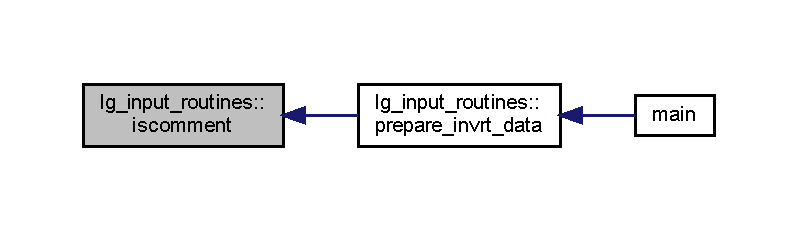
\includegraphics[width=350pt]{namespacelg__input__routines_a8433a2003dce3e9ebdd1aa0a11e16538_icgraph}
\end{center}
\end{figure}
\mbox{\Hypertarget{namespacelg__input__routines_a3118d974d52f2c98169709e887ceb344}\label{namespacelg__input__routines_a3118d974d52f2c98169709e887ceb344}} 
\index{lg\+\_\+input\+\_\+routines@{lg\+\_\+input\+\_\+routines}!prepare\+\_\+invrt\+\_\+data@{prepare\+\_\+invrt\+\_\+data}}
\index{prepare\+\_\+invrt\+\_\+data@{prepare\+\_\+invrt\+\_\+data}!lg\+\_\+input\+\_\+routines@{lg\+\_\+input\+\_\+routines}}
\subsubsection{\texorpdfstring{prepare\+\_\+invrt\+\_\+data()}{prepare\_invrt\_data()}}
{\footnotesize\ttfamily subroutine lg\+\_\+input\+\_\+routines\+::prepare\+\_\+invrt\+\_\+data (\begin{DoxyParamCaption}{ }\end{DoxyParamCaption})}

Here is the call graph for this function\+:\nopagebreak
\begin{figure}[H]
\begin{center}
\leavevmode
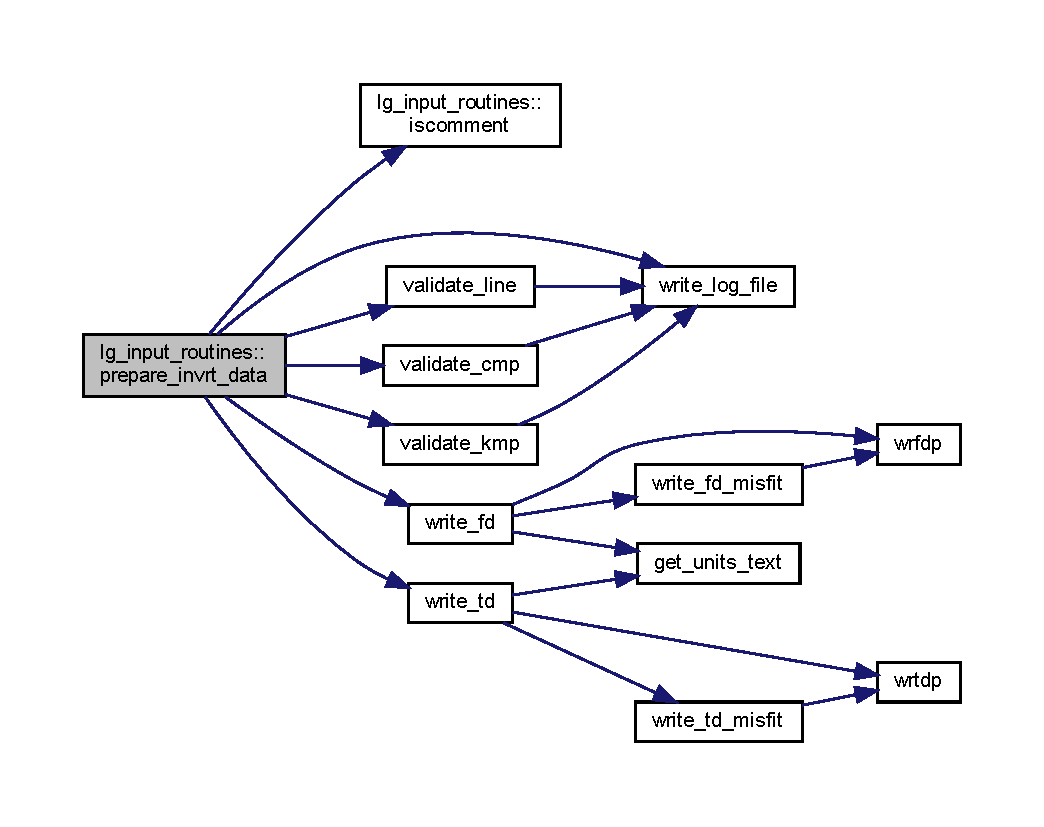
\includegraphics[width=350pt]{namespacelg__input__routines_a3118d974d52f2c98169709e887ceb344_cgraph}
\end{center}
\end{figure}
Here is the caller graph for this function\+:\nopagebreak
\begin{figure}[H]
\begin{center}
\leavevmode
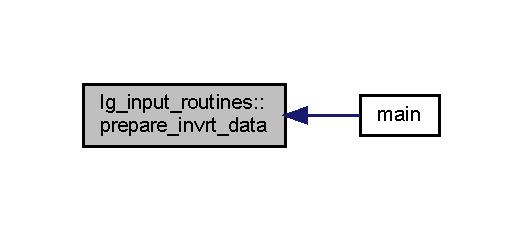
\includegraphics[width=251pt]{namespacelg__input__routines_a3118d974d52f2c98169709e887ceb344_icgraph}
\end{center}
\end{figure}
\mbox{\Hypertarget{namespacelg__input__routines_a39e1903280f0492197231ab5fa752f21}\label{namespacelg__input__routines_a39e1903280f0492197231ab5fa752f21}} 
\index{lg\+\_\+input\+\_\+routines@{lg\+\_\+input\+\_\+routines}!read\+\_\+model\+\_\+data@{read\+\_\+model\+\_\+data}}
\index{read\+\_\+model\+\_\+data@{read\+\_\+model\+\_\+data}!lg\+\_\+input\+\_\+routines@{lg\+\_\+input\+\_\+routines}}
\subsubsection{\texorpdfstring{read\+\_\+model\+\_\+data()}{read\_model\_data()}}
{\footnotesize\ttfamily subroutine lg\+\_\+input\+\_\+routines\+::read\+\_\+model\+\_\+data (\begin{DoxyParamCaption}{ }\end{DoxyParamCaption})}

Here is the call graph for this function\+:\nopagebreak
\begin{figure}[H]
\begin{center}
\leavevmode
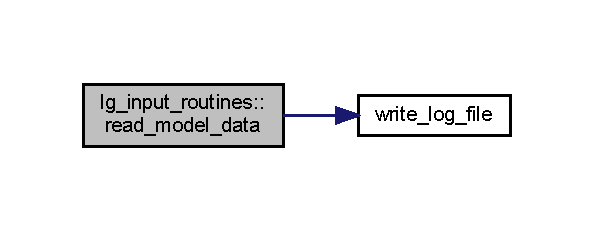
\includegraphics[width=285pt]{namespacelg__input__routines_a39e1903280f0492197231ab5fa752f21_cgraph}
\end{center}
\end{figure}
Here is the caller graph for this function\+:\nopagebreak
\begin{figure}[H]
\begin{center}
\leavevmode
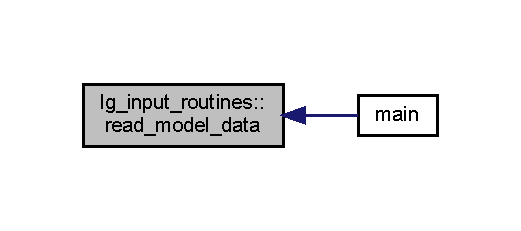
\includegraphics[width=250pt]{namespacelg__input__routines_a39e1903280f0492197231ab5fa752f21_icgraph}
\end{center}
\end{figure}
\mbox{\Hypertarget{namespacelg__input__routines_a123f91865ea388eca78b77b0d625aa8c}\label{namespacelg__input__routines_a123f91865ea388eca78b77b0d625aa8c}} 
\index{lg\+\_\+input\+\_\+routines@{lg\+\_\+input\+\_\+routines}!read\+\_\+parameter\+\_\+control@{read\+\_\+parameter\+\_\+control}}
\index{read\+\_\+parameter\+\_\+control@{read\+\_\+parameter\+\_\+control}!lg\+\_\+input\+\_\+routines@{lg\+\_\+input\+\_\+routines}}
\subsubsection{\texorpdfstring{read\+\_\+parameter\+\_\+control()}{read\_parameter\_control()}}
{\footnotesize\ttfamily subroutine lg\+\_\+input\+\_\+routines\+::read\+\_\+parameter\+\_\+control (\begin{DoxyParamCaption}{ }\end{DoxyParamCaption})}

Here is the call graph for this function\+:\nopagebreak
\begin{figure}[H]
\begin{center}
\leavevmode
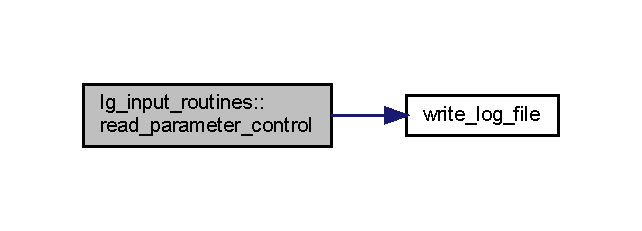
\includegraphics[width=308pt]{namespacelg__input__routines_a123f91865ea388eca78b77b0d625aa8c_cgraph}
\end{center}
\end{figure}
Here is the caller graph for this function\+:\nopagebreak
\begin{figure}[H]
\begin{center}
\leavevmode
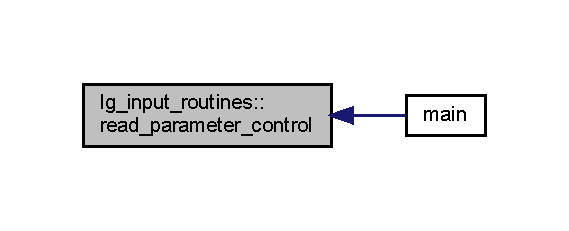
\includegraphics[width=273pt]{namespacelg__input__routines_a123f91865ea388eca78b77b0d625aa8c_icgraph}
\end{center}
\end{figure}
\mbox{\Hypertarget{namespacelg__input__routines_a80feb058541516d5a6327fb6c344bbbd}\label{namespacelg__input__routines_a80feb058541516d5a6327fb6c344bbbd}} 
\index{lg\+\_\+input\+\_\+routines@{lg\+\_\+input\+\_\+routines}!read\+\_\+system\+\_\+and\+\_\+survey\+\_\+data@{read\+\_\+system\+\_\+and\+\_\+survey\+\_\+data}}
\index{read\+\_\+system\+\_\+and\+\_\+survey\+\_\+data@{read\+\_\+system\+\_\+and\+\_\+survey\+\_\+data}!lg\+\_\+input\+\_\+routines@{lg\+\_\+input\+\_\+routines}}
\subsubsection{\texorpdfstring{read\+\_\+system\+\_\+and\+\_\+survey\+\_\+data()}{read\_system\_and\_survey\_data()}}
{\footnotesize\ttfamily subroutine lg\+\_\+input\+\_\+routines\+::read\+\_\+system\+\_\+and\+\_\+survey\+\_\+data (\begin{DoxyParamCaption}{ }\end{DoxyParamCaption})}

Here is the call graph for this function\+:\nopagebreak
\begin{figure}[H]
\begin{center}
\leavevmode
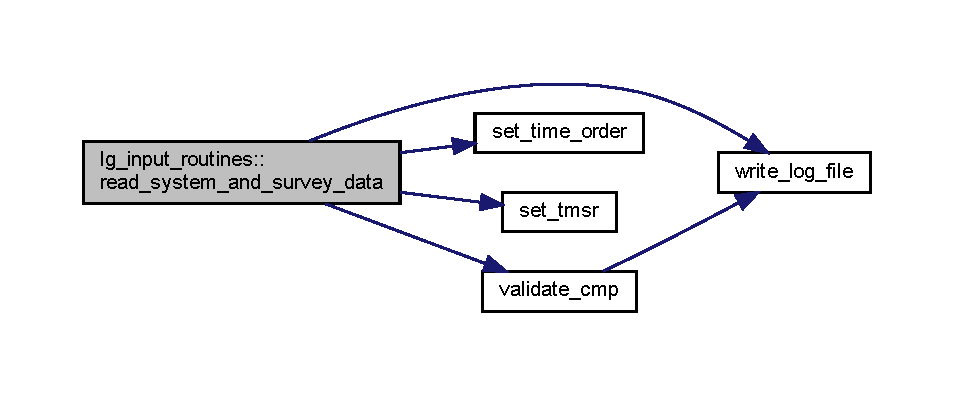
\includegraphics[width=350pt]{namespacelg__input__routines_a80feb058541516d5a6327fb6c344bbbd_cgraph}
\end{center}
\end{figure}
Here is the caller graph for this function\+:\nopagebreak
\begin{figure}[H]
\begin{center}
\leavevmode
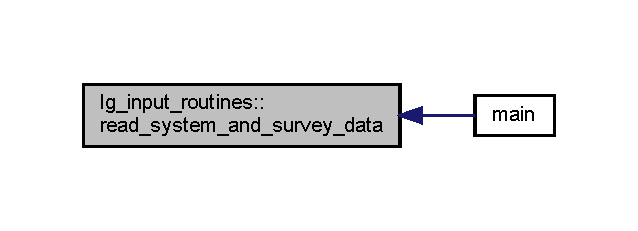
\includegraphics[width=306pt]{namespacelg__input__routines_a80feb058541516d5a6327fb6c344bbbd_icgraph}
\end{center}
\end{figure}
\mbox{\Hypertarget{namespacelg__input__routines_a836674acd30d52d3aa973722014aaa9f}\label{namespacelg__input__routines_a836674acd30d52d3aa973722014aaa9f}} 
\index{lg\+\_\+input\+\_\+routines@{lg\+\_\+input\+\_\+routines}!set\+\_\+frq@{set\+\_\+frq}}
\index{set\+\_\+frq@{set\+\_\+frq}!lg\+\_\+input\+\_\+routines@{lg\+\_\+input\+\_\+routines}}
\subsubsection{\texorpdfstring{set\+\_\+frq()}{set\_frq()}}
{\footnotesize\ttfamily subroutine lg\+\_\+input\+\_\+routines\+::set\+\_\+frq (\begin{DoxyParamCaption}{ }\end{DoxyParamCaption})}

Here is the caller graph for this function\+:\nopagebreak
\begin{figure}[H]
\begin{center}
\leavevmode
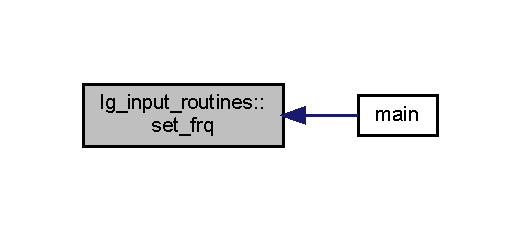
\includegraphics[width=250pt]{namespacelg__input__routines_a836674acd30d52d3aa973722014aaa9f_icgraph}
\end{center}
\end{figure}
\mbox{\Hypertarget{namespacelg__input__routines_a74107bd43614b32d8679e91def53e94d}\label{namespacelg__input__routines_a74107bd43614b32d8679e91def53e94d}} 
\index{lg\+\_\+input\+\_\+routines@{lg\+\_\+input\+\_\+routines}!set\+\_\+rho@{set\+\_\+rho}}
\index{set\+\_\+rho@{set\+\_\+rho}!lg\+\_\+input\+\_\+routines@{lg\+\_\+input\+\_\+routines}}
\subsubsection{\texorpdfstring{set\+\_\+rho()}{set\_rho()}}
{\footnotesize\ttfamily subroutine lg\+\_\+input\+\_\+routines\+::set\+\_\+rho (\begin{DoxyParamCaption}{ }\end{DoxyParamCaption})}

Here is the caller graph for this function\+:\nopagebreak
\begin{figure}[H]
\begin{center}
\leavevmode
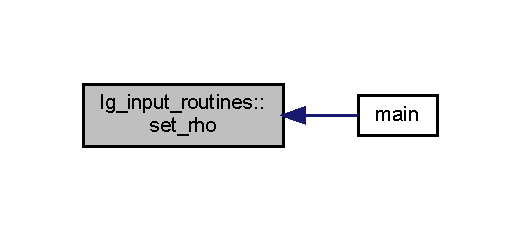
\includegraphics[width=250pt]{namespacelg__input__routines_a74107bd43614b32d8679e91def53e94d_icgraph}
\end{center}
\end{figure}
\mbox{\Hypertarget{namespacelg__input__routines_aff8e77512771c5a25793784a8185d5b0}\label{namespacelg__input__routines_aff8e77512771c5a25793784a8185d5b0}} 
\index{lg\+\_\+input\+\_\+routines@{lg\+\_\+input\+\_\+routines}!set\+\_\+trp@{set\+\_\+trp}}
\index{set\+\_\+trp@{set\+\_\+trp}!lg\+\_\+input\+\_\+routines@{lg\+\_\+input\+\_\+routines}}
\subsubsection{\texorpdfstring{set\+\_\+trp()}{set\_trp()}}
{\footnotesize\ttfamily subroutine lg\+\_\+input\+\_\+routines\+::set\+\_\+trp (\begin{DoxyParamCaption}{ }\end{DoxyParamCaption})}

Here is the caller graph for this function\+:\nopagebreak
\begin{figure}[H]
\begin{center}
\leavevmode
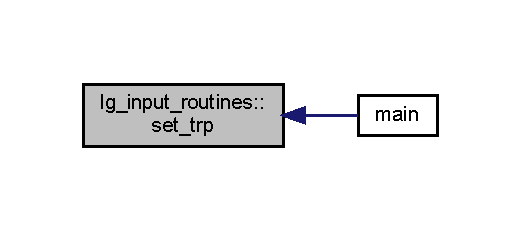
\includegraphics[width=250pt]{namespacelg__input__routines_aff8e77512771c5a25793784a8185d5b0_icgraph}
\end{center}
\end{figure}
\mbox{\Hypertarget{namespacelg__input__routines_a46a4ddc163c46adad59e863dadde86a3}\label{namespacelg__input__routines_a46a4ddc163c46adad59e863dadde86a3}} 
\index{lg\+\_\+input\+\_\+routines@{lg\+\_\+input\+\_\+routines}!show\+\_\+and\+\_\+tell@{show\+\_\+and\+\_\+tell}}
\index{show\+\_\+and\+\_\+tell@{show\+\_\+and\+\_\+tell}!lg\+\_\+input\+\_\+routines@{lg\+\_\+input\+\_\+routines}}
\subsubsection{\texorpdfstring{show\+\_\+and\+\_\+tell()}{show\_and\_tell()}}
{\footnotesize\ttfamily subroutine lg\+\_\+input\+\_\+routines\+::show\+\_\+and\+\_\+tell (\begin{DoxyParamCaption}{ }\end{DoxyParamCaption})}

Here is the call graph for this function\+:\nopagebreak
\begin{figure}[H]
\begin{center}
\leavevmode
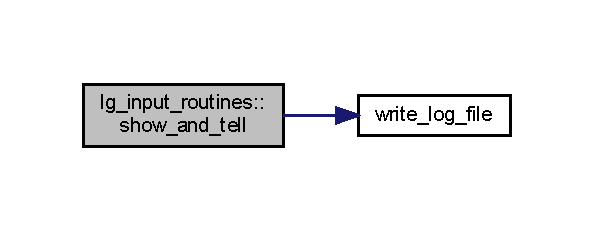
\includegraphics[width=285pt]{namespacelg__input__routines_a46a4ddc163c46adad59e863dadde86a3_cgraph}
\end{center}
\end{figure}
\mbox{\Hypertarget{namespacelg__input__routines_abb4589f0c8ad2d2d88f0f52aac5462e6}\label{namespacelg__input__routines_abb4589f0c8ad2d2d88f0f52aac5462e6}} 
\index{lg\+\_\+input\+\_\+routines@{lg\+\_\+input\+\_\+routines}!write\+\_\+line\+\_\+header@{write\+\_\+line\+\_\+header}}
\index{write\+\_\+line\+\_\+header@{write\+\_\+line\+\_\+header}!lg\+\_\+input\+\_\+routines@{lg\+\_\+input\+\_\+routines}}
\subsubsection{\texorpdfstring{write\+\_\+line\+\_\+header()}{write\_line\_header()}}
{\footnotesize\ttfamily subroutine lg\+\_\+input\+\_\+routines\+::write\+\_\+line\+\_\+header (\begin{DoxyParamCaption}\item[{character(len=20)}]{QL,  }\item[{integer}]{H\+ID,  }\item[{integer}]{CL,  }\item[{integer}]{N\+CL }\end{DoxyParamCaption})}

Here is the call graph for this function\+:\nopagebreak
\begin{figure}[H]
\begin{center}
\leavevmode
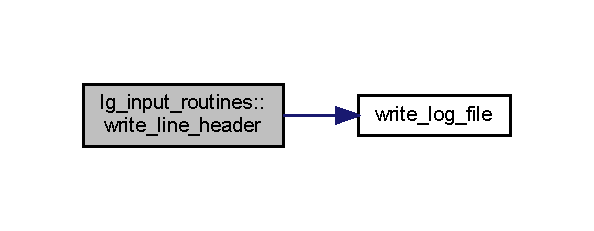
\includegraphics[width=285pt]{namespacelg__input__routines_abb4589f0c8ad2d2d88f0f52aac5462e6_cgraph}
\end{center}
\end{figure}
Here is the caller graph for this function\+:\nopagebreak
\begin{figure}[H]
\begin{center}
\leavevmode
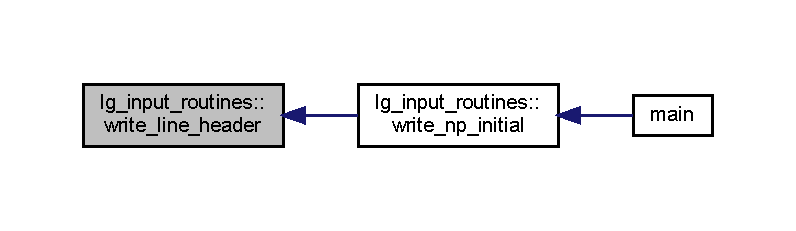
\includegraphics[width=350pt]{namespacelg__input__routines_abb4589f0c8ad2d2d88f0f52aac5462e6_icgraph}
\end{center}
\end{figure}
\mbox{\Hypertarget{namespacelg__input__routines_a1e34012960c952d22446828d97881001}\label{namespacelg__input__routines_a1e34012960c952d22446828d97881001}} 
\index{lg\+\_\+input\+\_\+routines@{lg\+\_\+input\+\_\+routines}!write\+\_\+np\+\_\+initial@{write\+\_\+np\+\_\+initial}}
\index{write\+\_\+np\+\_\+initial@{write\+\_\+np\+\_\+initial}!lg\+\_\+input\+\_\+routines@{lg\+\_\+input\+\_\+routines}}
\subsubsection{\texorpdfstring{write\+\_\+np\+\_\+initial()}{write\_np\_initial()}}
{\footnotesize\ttfamily subroutine lg\+\_\+input\+\_\+routines\+::write\+\_\+np\+\_\+initial (\begin{DoxyParamCaption}{ }\end{DoxyParamCaption})}

Here is the call graph for this function\+:\nopagebreak
\begin{figure}[H]
\begin{center}
\leavevmode
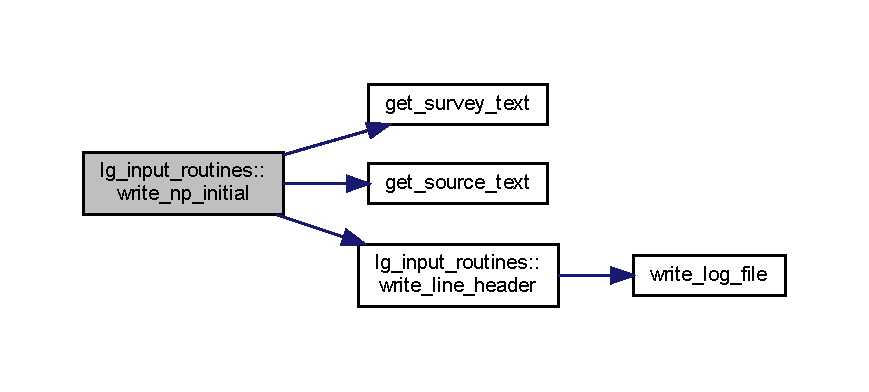
\includegraphics[width=350pt]{namespacelg__input__routines_a1e34012960c952d22446828d97881001_cgraph}
\end{center}
\end{figure}
Here is the caller graph for this function\+:\nopagebreak
\begin{figure}[H]
\begin{center}
\leavevmode
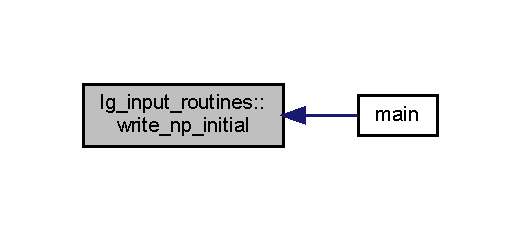
\includegraphics[width=250pt]{namespacelg__input__routines_a1e34012960c952d22446828d97881001_icgraph}
\end{center}
\end{figure}


\subsection{Variable Documentation}
\mbox{\Hypertarget{namespacelg__input__routines_ad240d679ecd403cc52aac764201bfc5b}\label{namespacelg__input__routines_ad240d679ecd403cc52aac764201bfc5b}} 
\index{lg\+\_\+input\+\_\+routines@{lg\+\_\+input\+\_\+routines}!beg@{beg}}
\index{beg@{beg}!lg\+\_\+input\+\_\+routines@{lg\+\_\+input\+\_\+routines}}
\subsubsection{\texorpdfstring{beg}{beg}}
{\footnotesize\ttfamily integer lg\+\_\+input\+\_\+routines\+::beg}

\mbox{\Hypertarget{namespacelg__input__routines_ac7f5afd80317e5c4f20d0f68bac9cf59}\label{namespacelg__input__routines_ac7f5afd80317e5c4f20d0f68bac9cf59}} 
\index{lg\+\_\+input\+\_\+routines@{lg\+\_\+input\+\_\+routines}!bftl@{bftl}}
\index{bftl@{bftl}!lg\+\_\+input\+\_\+routines@{lg\+\_\+input\+\_\+routines}}
\subsubsection{\texorpdfstring{bftl}{bftl}}
{\footnotesize\ttfamily real, dimension(\+:,\+:,\+:,\+:), allocatable lg\+\_\+input\+\_\+routines\+::bftl}

\mbox{\Hypertarget{namespacelg__input__routines_aaddc398e9198a4c9e8eb40573a3f4347}\label{namespacelg__input__routines_aaddc398e9198a4c9e8eb40573a3f4347}} 
\index{lg\+\_\+input\+\_\+routines@{lg\+\_\+input\+\_\+routines}!bhazm@{bhazm}}
\index{bhazm@{bhazm}!lg\+\_\+input\+\_\+routines@{lg\+\_\+input\+\_\+routines}}
\subsubsection{\texorpdfstring{bhazm}{bhazm}}
{\footnotesize\ttfamily real, dimension(\+:,\+:), allocatable lg\+\_\+input\+\_\+routines\+::bhazm}

\mbox{\Hypertarget{namespacelg__input__routines_ad18dca12a7805ae624b71667a773a294}\label{namespacelg__input__routines_ad18dca12a7805ae624b71667a773a294}} 
\index{lg\+\_\+input\+\_\+routines@{lg\+\_\+input\+\_\+routines}!bhdip@{bhdip}}
\index{bhdip@{bhdip}!lg\+\_\+input\+\_\+routines@{lg\+\_\+input\+\_\+routines}}
\subsubsection{\texorpdfstring{bhdip}{bhdip}}
{\footnotesize\ttfamily real, dimension(\+:,\+:), allocatable lg\+\_\+input\+\_\+routines\+::bhdip}

\mbox{\Hypertarget{namespacelg__input__routines_a5aaa08577983b3738ea36301b56c0410}\label{namespacelg__input__routines_a5aaa08577983b3738ea36301b56c0410}} 
\index{lg\+\_\+input\+\_\+routines@{lg\+\_\+input\+\_\+routines}!cellw@{cellw}}
\index{cellw@{cellw}!lg\+\_\+input\+\_\+routines@{lg\+\_\+input\+\_\+routines}}
\subsubsection{\texorpdfstring{cellw}{cellw}}
{\footnotesize\ttfamily real lg\+\_\+input\+\_\+routines\+::cellw}

\mbox{\Hypertarget{namespacelg__input__routines_aa9fa43a162e95877320d121ab31b958d}\label{namespacelg__input__routines_aa9fa43a162e95877320d121ab31b958d}} 
\index{lg\+\_\+input\+\_\+routines@{lg\+\_\+input\+\_\+routines}!cfreq@{cfreq}}
\index{cfreq@{cfreq}!lg\+\_\+input\+\_\+routines@{lg\+\_\+input\+\_\+routines}}
\subsubsection{\texorpdfstring{cfreq}{cfreq}}
{\footnotesize\ttfamily real, dimension(\+:), allocatable lg\+\_\+input\+\_\+routines\+::cfreq}

\mbox{\Hypertarget{namespacelg__input__routines_a39583b1655c1a6964d1e80639879060b}\label{namespacelg__input__routines_a39583b1655c1a6964d1e80639879060b}} 
\index{lg\+\_\+input\+\_\+routines@{lg\+\_\+input\+\_\+routines}!cfreqp@{cfreqp}}
\index{cfreqp@{cfreqp}!lg\+\_\+input\+\_\+routines@{lg\+\_\+input\+\_\+routines}}
\subsubsection{\texorpdfstring{cfreqp}{cfreqp}}
{\footnotesize\ttfamily real, dimension(\+:), allocatable lg\+\_\+input\+\_\+routines\+::cfreqp}

\mbox{\Hypertarget{namespacelg__input__routines_a1653ca16fcac1be1d1e8449d3bcea089}\label{namespacelg__input__routines_a1653ca16fcac1be1d1e8449d3bcea089}} 
\index{lg\+\_\+input\+\_\+routines@{lg\+\_\+input\+\_\+routines}!chrg@{chrg}}
\index{chrg@{chrg}!lg\+\_\+input\+\_\+routines@{lg\+\_\+input\+\_\+routines}}
\subsubsection{\texorpdfstring{chrg}{chrg}}
{\footnotesize\ttfamily real, dimension(\+:), allocatable lg\+\_\+input\+\_\+routines\+::chrg}

\mbox{\Hypertarget{namespacelg__input__routines_a05b7b31b77371774e886aadf410be79e}\label{namespacelg__input__routines_a05b7b31b77371774e886aadf410be79e}} 
\index{lg\+\_\+input\+\_\+routines@{lg\+\_\+input\+\_\+routines}!chrgp@{chrgp}}
\index{chrgp@{chrgp}!lg\+\_\+input\+\_\+routines@{lg\+\_\+input\+\_\+routines}}
\subsubsection{\texorpdfstring{chrgp}{chrgp}}
{\footnotesize\ttfamily real, dimension(\+:), allocatable lg\+\_\+input\+\_\+routines\+::chrgp}

\mbox{\Hypertarget{namespacelg__input__routines_ae8692e647d0f89e881c118c611840cd9}\label{namespacelg__input__routines_ae8692e647d0f89e881c118c611840cd9}} 
\index{lg\+\_\+input\+\_\+routines@{lg\+\_\+input\+\_\+routines}!clcd@{clcd}}
\index{clcd@{clcd}!lg\+\_\+input\+\_\+routines@{lg\+\_\+input\+\_\+routines}}
\subsubsection{\texorpdfstring{clcd}{clcd}}
{\footnotesize\ttfamily real(kind=\hyperlink{namespacelg__input__routines_a8c3fd17aa03dd450ed3e242df939ad01}{ql}), dimension(\+:,\+:), allocatable lg\+\_\+input\+\_\+routines\+::clcd}

\mbox{\Hypertarget{namespacelg__input__routines_ae700c1a68129dc3b61dd0eee2253b79f}\label{namespacelg__input__routines_ae700c1a68129dc3b61dd0eee2253b79f}} 
\index{lg\+\_\+input\+\_\+routines@{lg\+\_\+input\+\_\+routines}!cmp@{cmp}}
\index{cmp@{cmp}!lg\+\_\+input\+\_\+routines@{lg\+\_\+input\+\_\+routines}}
\subsubsection{\texorpdfstring{cmp}{cmp}}
{\footnotesize\ttfamily integer, dimension(\+:), allocatable lg\+\_\+input\+\_\+routines\+::cmp}

\mbox{\Hypertarget{namespacelg__input__routines_aa1e90821ade680361e1ae7f091fe973b}\label{namespacelg__input__routines_aa1e90821ade680361e1ae7f091fe973b}} 
\index{lg\+\_\+input\+\_\+routines@{lg\+\_\+input\+\_\+routines}!cmpmt@{cmpmt}}
\index{cmpmt@{cmpmt}!lg\+\_\+input\+\_\+routines@{lg\+\_\+input\+\_\+routines}}
\subsubsection{\texorpdfstring{cmpmt}{cmpmt}}
{\footnotesize\ttfamily integer, dimension(4) lg\+\_\+input\+\_\+routines\+::cmpmt}

\mbox{\Hypertarget{namespacelg__input__routines_aa67064f3118bc318702e1ca97b197a05}\label{namespacelg__input__routines_aa67064f3118bc318702e1ca97b197a05}} 
\index{lg\+\_\+input\+\_\+routines@{lg\+\_\+input\+\_\+routines}!cnvrg@{cnvrg}}
\index{cnvrg@{cnvrg}!lg\+\_\+input\+\_\+routines@{lg\+\_\+input\+\_\+routines}}
\subsubsection{\texorpdfstring{cnvrg}{cnvrg}}
{\footnotesize\ttfamily integer lg\+\_\+input\+\_\+routines\+::cnvrg}

\mbox{\Hypertarget{namespacelg__input__routines_ac8bb200fd8bf044a20d5445759fab02c}\label{namespacelg__input__routines_ac8bb200fd8bf044a20d5445759fab02c}} 
\index{lg\+\_\+input\+\_\+routines@{lg\+\_\+input\+\_\+routines}!ctau@{ctau}}
\index{ctau@{ctau}!lg\+\_\+input\+\_\+routines@{lg\+\_\+input\+\_\+routines}}
\subsubsection{\texorpdfstring{ctau}{ctau}}
{\footnotesize\ttfamily real, dimension(\+:), allocatable lg\+\_\+input\+\_\+routines\+::ctau}

\mbox{\Hypertarget{namespacelg__input__routines_a4ca057c77a03e564a388368be839cd43}\label{namespacelg__input__routines_a4ca057c77a03e564a388368be839cd43}} 
\index{lg\+\_\+input\+\_\+routines@{lg\+\_\+input\+\_\+routines}!ctaup@{ctaup}}
\index{ctaup@{ctaup}!lg\+\_\+input\+\_\+routines@{lg\+\_\+input\+\_\+routines}}
\subsubsection{\texorpdfstring{ctaup}{ctaup}}
{\footnotesize\ttfamily real, dimension(\+:), allocatable lg\+\_\+input\+\_\+routines\+::ctaup}

\mbox{\Hypertarget{namespacelg__input__routines_a2724872da9ddfe9b94de8c091b0a36dd}\label{namespacelg__input__routines_a2724872da9ddfe9b94de8c091b0a36dd}} 
\index{lg\+\_\+input\+\_\+routines@{lg\+\_\+input\+\_\+routines}!curnt@{curnt}}
\index{curnt@{curnt}!lg\+\_\+input\+\_\+routines@{lg\+\_\+input\+\_\+routines}}
\subsubsection{\texorpdfstring{curnt}{curnt}}
{\footnotesize\ttfamily real, dimension(\+:), allocatable lg\+\_\+input\+\_\+routines\+::curnt}

\mbox{\Hypertarget{namespacelg__input__routines_aa1ea996394cf4a5e7b496595554acf71}\label{namespacelg__input__routines_aa1ea996394cf4a5e7b496595554acf71}} 
\index{lg\+\_\+input\+\_\+routines@{lg\+\_\+input\+\_\+routines}!cxpar@{cxpar}}
\index{cxpar@{cxpar}!lg\+\_\+input\+\_\+routines@{lg\+\_\+input\+\_\+routines}}
\subsubsection{\texorpdfstring{cxpar}{cxpar}}
{\footnotesize\ttfamily integer, dimension(\+:), allocatable lg\+\_\+input\+\_\+routines\+::cxpar}

\mbox{\Hypertarget{namespacelg__input__routines_a17c7af951ca7d0cf40e35d63cadf6d43}\label{namespacelg__input__routines_a17c7af951ca7d0cf40e35d63cadf6d43}} 
\index{lg\+\_\+input\+\_\+routines@{lg\+\_\+input\+\_\+routines}!d2r@{d2r}}
\index{d2r@{d2r}!lg\+\_\+input\+\_\+routines@{lg\+\_\+input\+\_\+routines}}
\subsubsection{\texorpdfstring{d2r}{d2r}}
{\footnotesize\ttfamily real parameter lg\+\_\+input\+\_\+routines\+::d2r =PI/180.}

\mbox{\Hypertarget{namespacelg__input__routines_ac11fcc9d6ce359143f3e92b12bc56633}\label{namespacelg__input__routines_ac11fcc9d6ce359143f3e92b12bc56633}} 
\index{lg\+\_\+input\+\_\+routines@{lg\+\_\+input\+\_\+routines}!dip@{dip}}
\index{dip@{dip}!lg\+\_\+input\+\_\+routines@{lg\+\_\+input\+\_\+routines}}
\subsubsection{\texorpdfstring{dip}{dip}}
{\footnotesize\ttfamily real, dimension(\+:), allocatable lg\+\_\+input\+\_\+routines\+::dip}

\mbox{\Hypertarget{namespacelg__input__routines_af78f7591d1f55c4a9a6aec78bdafb61c}\label{namespacelg__input__routines_af78f7591d1f55c4a9a6aec78bdafb61c}} 
\index{lg\+\_\+input\+\_\+routines@{lg\+\_\+input\+\_\+routines}!do3d@{do3d}}
\index{do3d@{do3d}!lg\+\_\+input\+\_\+routines@{lg\+\_\+input\+\_\+routines}}
\subsubsection{\texorpdfstring{do3d}{do3d}}
{\footnotesize\ttfamily integer lg\+\_\+input\+\_\+routines\+::do3d}

\mbox{\Hypertarget{namespacelg__input__routines_a0ad3fab990ff61df0aef4ca7bb41cf23}\label{namespacelg__input__routines_a0ad3fab990ff61df0aef4ca7bb41cf23}} 
\index{lg\+\_\+input\+\_\+routines@{lg\+\_\+input\+\_\+routines}!dstat@{dstat}}
\index{dstat@{dstat}!lg\+\_\+input\+\_\+routines@{lg\+\_\+input\+\_\+routines}}
\subsubsection{\texorpdfstring{dstat}{dstat}}
{\footnotesize\ttfamily real, dimension(\+:,\+:), allocatable lg\+\_\+input\+\_\+routines\+::dstat}

\mbox{\Hypertarget{namespacelg__input__routines_ac8e6a73637bd5b85bdfbfc0734b3e44a}\label{namespacelg__input__routines_ac8e6a73637bd5b85bdfbfc0734b3e44a}} 
\index{lg\+\_\+input\+\_\+routines@{lg\+\_\+input\+\_\+routines}!dzm@{dzm}}
\index{dzm@{dzm}!lg\+\_\+input\+\_\+routines@{lg\+\_\+input\+\_\+routines}}
\subsubsection{\texorpdfstring{dzm}{dzm}}
{\footnotesize\ttfamily real, dimension(\+:), allocatable lg\+\_\+input\+\_\+routines\+::dzm}

\mbox{\Hypertarget{namespacelg__input__routines_a324ba9df6f9ed5b8c67035350579f985}\label{namespacelg__input__routines_a324ba9df6f9ed5b8c67035350579f985}} 
\index{lg\+\_\+input\+\_\+routines@{lg\+\_\+input\+\_\+routines}!ecntrd@{ecntrd}}
\index{ecntrd@{ecntrd}!lg\+\_\+input\+\_\+routines@{lg\+\_\+input\+\_\+routines}}
\subsubsection{\texorpdfstring{ecntrd}{ecntrd}}
{\footnotesize\ttfamily real(kind=\hyperlink{namespacelg__input__routines_a8c3fd17aa03dd450ed3e242df939ad01}{ql}) lg\+\_\+input\+\_\+routines\+::ecntrd}

\mbox{\Hypertarget{namespacelg__input__routines_a45d7d9feedc943e6eeb7c96241a56cb9}\label{namespacelg__input__routines_a45d7d9feedc943e6eeb7c96241a56cb9}} 
\index{lg\+\_\+input\+\_\+routines@{lg\+\_\+input\+\_\+routines}!elas@{elas}}
\index{elas@{elas}!lg\+\_\+input\+\_\+routines@{lg\+\_\+input\+\_\+routines}}
\subsubsection{\texorpdfstring{elas}{elas}}
{\footnotesize\ttfamily real, dimension(\+:), allocatable lg\+\_\+input\+\_\+routines\+::elas}

\mbox{\Hypertarget{namespacelg__input__routines_a67371f9c06d68b95d45184555688f5da}\label{namespacelg__input__routines_a67371f9c06d68b95d45184555688f5da}} 
\index{lg\+\_\+input\+\_\+routines@{lg\+\_\+input\+\_\+routines}!fin@{fin}}
\index{fin@{fin}!lg\+\_\+input\+\_\+routines@{lg\+\_\+input\+\_\+routines}}
\subsubsection{\texorpdfstring{fin}{fin}}
{\footnotesize\ttfamily integer lg\+\_\+input\+\_\+routines\+::fin}

\mbox{\Hypertarget{namespacelg__input__routines_a8482cf4c4f82b0bdade2229ebe84409b}\label{namespacelg__input__routines_a8482cf4c4f82b0bdade2229ebe84409b}} 
\index{lg\+\_\+input\+\_\+routines@{lg\+\_\+input\+\_\+routines}!fqq@{fqq}}
\index{fqq@{fqq}!lg\+\_\+input\+\_\+routines@{lg\+\_\+input\+\_\+routines}}
\subsubsection{\texorpdfstring{fqq}{fqq}}
{\footnotesize\ttfamily real(kind=\hyperlink{namespacelg__input__routines_a8c3fd17aa03dd450ed3e242df939ad01}{ql}) lg\+\_\+input\+\_\+routines\+::fqq}

\mbox{\Hypertarget{namespacelg__input__routines_a2c092becc43cb2313a011cc8e3962349}\label{namespacelg__input__routines_a2c092becc43cb2313a011cc8e3962349}} 
\index{lg\+\_\+input\+\_\+routines@{lg\+\_\+input\+\_\+routines}!freq@{freq}}
\index{freq@{freq}!lg\+\_\+input\+\_\+routines@{lg\+\_\+input\+\_\+routines}}
\subsubsection{\texorpdfstring{freq}{freq}}
{\footnotesize\ttfamily real, dimension(\+:), allocatable lg\+\_\+input\+\_\+routines\+::freq}

\mbox{\Hypertarget{namespacelg__input__routines_ad64edbbe93c0335e2a4d4d767eb9bbd1}\label{namespacelg__input__routines_ad64edbbe93c0335e2a4d4d767eb9bbd1}} 
\index{lg\+\_\+input\+\_\+routines@{lg\+\_\+input\+\_\+routines}!fvers@{fvers}}
\index{fvers@{fvers}!lg\+\_\+input\+\_\+routines@{lg\+\_\+input\+\_\+routines}}
\subsubsection{\texorpdfstring{fvers}{fvers}}
{\footnotesize\ttfamily integer parameter lg\+\_\+input\+\_\+routines\+::fvers = 690}

\mbox{\Hypertarget{namespacelg__input__routines_a84a9e4845e4cff7e15d920d545e920fe}\label{namespacelg__input__routines_a84a9e4845e4cff7e15d920d545e920fe}} 
\index{lg\+\_\+input\+\_\+routines@{lg\+\_\+input\+\_\+routines}!header\+\_\+id@{header\+\_\+id}}
\index{header\+\_\+id@{header\+\_\+id}!lg\+\_\+input\+\_\+routines@{lg\+\_\+input\+\_\+routines}}
\subsubsection{\texorpdfstring{header\+\_\+id}{header\_id}}
{\footnotesize\ttfamily integer, dimension(\+:), allocatable lg\+\_\+input\+\_\+routines\+::header\+\_\+id}

\mbox{\Hypertarget{namespacelg__input__routines_a25ef99b6df9850605ad2562a20d87711}\label{namespacelg__input__routines_a25ef99b6df9850605ad2562a20d87711}} 
\index{lg\+\_\+input\+\_\+routines@{lg\+\_\+input\+\_\+routines}!idh@{idh}}
\index{idh@{idh}!lg\+\_\+input\+\_\+routines@{lg\+\_\+input\+\_\+routines}}
\subsubsection{\texorpdfstring{idh}{idh}}
{\footnotesize\ttfamily integer, dimension(\+:), allocatable lg\+\_\+input\+\_\+routines\+::idh}

\mbox{\Hypertarget{namespacelg__input__routines_a288298e67f0d988bf7778f7d3e647080}\label{namespacelg__input__routines_a288298e67f0d988bf7778f7d3e647080}} 
\index{lg\+\_\+input\+\_\+routines@{lg\+\_\+input\+\_\+routines}!inp@{inp}}
\index{inp@{inp}!lg\+\_\+input\+\_\+routines@{lg\+\_\+input\+\_\+routines}}
\subsubsection{\texorpdfstring{inp}{inp}}
{\footnotesize\ttfamily character (len=200) lg\+\_\+input\+\_\+routines\+::inp}

\mbox{\Hypertarget{namespacelg__input__routines_a24ada50400969251dbef61f7706a66cc}\label{namespacelg__input__routines_a24ada50400969251dbef61f7706a66cc}} 
\index{lg\+\_\+input\+\_\+routines@{lg\+\_\+input\+\_\+routines}!intrude@{intrude}}
\index{intrude@{intrude}!lg\+\_\+input\+\_\+routines@{lg\+\_\+input\+\_\+routines}}
\subsubsection{\texorpdfstring{intrude}{intrude}}
{\footnotesize\ttfamily logical lg\+\_\+input\+\_\+routines\+::intrude}

\mbox{\Hypertarget{namespacelg__input__routines_a8a8f780e770a419032c0f864583b10b3}\label{namespacelg__input__routines_a8a8f780e770a419032c0f864583b10b3}} 
\index{lg\+\_\+input\+\_\+routines@{lg\+\_\+input\+\_\+routines}!invert@{invert}}
\index{invert@{invert}!lg\+\_\+input\+\_\+routines@{lg\+\_\+input\+\_\+routines}}
\subsubsection{\texorpdfstring{invert}{invert}}
{\footnotesize\ttfamily logical lg\+\_\+input\+\_\+routines\+::invert}

\mbox{\Hypertarget{namespacelg__input__routines_a2efdd9d0ee189172094271241f63d28c}\label{namespacelg__input__routines_a2efdd9d0ee189172094271241f63d28c}} 
\index{lg\+\_\+input\+\_\+routines@{lg\+\_\+input\+\_\+routines}!invprt@{invprt}}
\index{invprt@{invprt}!lg\+\_\+input\+\_\+routines@{lg\+\_\+input\+\_\+routines}}
\subsubsection{\texorpdfstring{invprt}{invprt}}
{\footnotesize\ttfamily integer lg\+\_\+input\+\_\+routines\+::invprt}

\mbox{\Hypertarget{namespacelg__input__routines_a7ac8905ebcdb83c2e30359605834b350}\label{namespacelg__input__routines_a7ac8905ebcdb83c2e30359605834b350}} 
\index{lg\+\_\+input\+\_\+routines@{lg\+\_\+input\+\_\+routines}!iplt@{iplt}}
\index{iplt@{iplt}!lg\+\_\+input\+\_\+routines@{lg\+\_\+input\+\_\+routines}}
\subsubsection{\texorpdfstring{iplt}{iplt}}
{\footnotesize\ttfamily integer, dimension(\+:), allocatable lg\+\_\+input\+\_\+routines\+::iplt}

\mbox{\Hypertarget{namespacelg__input__routines_a4eb4ee97a7b4d0a162e4c92b3c592678}\label{namespacelg__input__routines_a4eb4ee97a7b4d0a162e4c92b3c592678}} 
\index{lg\+\_\+input\+\_\+routines@{lg\+\_\+input\+\_\+routines}!ippd@{ippd}}
\index{ippd@{ippd}!lg\+\_\+input\+\_\+routines@{lg\+\_\+input\+\_\+routines}}
\subsubsection{\texorpdfstring{ippd}{ippd}}
{\footnotesize\ttfamily integer lg\+\_\+input\+\_\+routines\+::ippd}

\mbox{\Hypertarget{namespacelg__input__routines_a23b2611e5e3842861e03d1b579dc49aa}\label{namespacelg__input__routines_a23b2611e5e3842861e03d1b579dc49aa}} 
\index{lg\+\_\+input\+\_\+routines@{lg\+\_\+input\+\_\+routines}!istop@{istop}}
\index{istop@{istop}!lg\+\_\+input\+\_\+routines@{lg\+\_\+input\+\_\+routines}}
\subsubsection{\texorpdfstring{istop}{istop}}
{\footnotesize\ttfamily integer lg\+\_\+input\+\_\+routines\+::istop}

\mbox{\Hypertarget{namespacelg__input__routines_a21d152072d7a9e7973cbbe660dad9e88}\label{namespacelg__input__routines_a21d152072d7a9e7973cbbe660dad9e88}} 
\index{lg\+\_\+input\+\_\+routines@{lg\+\_\+input\+\_\+routines}!isys@{isys}}
\index{isys@{isys}!lg\+\_\+input\+\_\+routines@{lg\+\_\+input\+\_\+routines}}
\subsubsection{\texorpdfstring{isys}{isys}}
{\footnotesize\ttfamily integer lg\+\_\+input\+\_\+routines\+::isys}

\mbox{\Hypertarget{namespacelg__input__routines_a78d4457ced9beccb65b6782146533a24}\label{namespacelg__input__routines_a78d4457ced9beccb65b6782146533a24}} 
\index{lg\+\_\+input\+\_\+routines@{lg\+\_\+input\+\_\+routines}!j@{j}}
\index{j@{j}!lg\+\_\+input\+\_\+routines@{lg\+\_\+input\+\_\+routines}}
\subsubsection{\texorpdfstring{j}{j}}
{\footnotesize\ttfamily integer lg\+\_\+input\+\_\+routines\+::j}

\mbox{\Hypertarget{namespacelg__input__routines_aee9292c01f55d537f7cafc9a3e5201bf}\label{namespacelg__input__routines_aee9292c01f55d537f7cafc9a3e5201bf}} 
\index{lg\+\_\+input\+\_\+routines@{lg\+\_\+input\+\_\+routines}!ja@{ja}}
\index{ja@{ja}!lg\+\_\+input\+\_\+routines@{lg\+\_\+input\+\_\+routines}}
\subsubsection{\texorpdfstring{ja}{ja}}
{\footnotesize\ttfamily integer lg\+\_\+input\+\_\+routines\+::ja}

\mbox{\Hypertarget{namespacelg__input__routines_a2b02a6181257c199eba71b3c92fb5be9}\label{namespacelg__input__routines_a2b02a6181257c199eba71b3c92fb5be9}} 
\index{lg\+\_\+input\+\_\+routines@{lg\+\_\+input\+\_\+routines}!jab@{jab}}
\index{jab@{jab}!lg\+\_\+input\+\_\+routines@{lg\+\_\+input\+\_\+routines}}
\subsubsection{\texorpdfstring{jab}{jab}}
{\footnotesize\ttfamily integer lg\+\_\+input\+\_\+routines\+::jab}

\mbox{\Hypertarget{namespacelg__input__routines_aa8dab0fb04a941c104a2358b9964b3cb}\label{namespacelg__input__routines_aa8dab0fb04a941c104a2358b9964b3cb}} 
\index{lg\+\_\+input\+\_\+routines@{lg\+\_\+input\+\_\+routines}!jab2@{jab2}}
\index{jab2@{jab2}!lg\+\_\+input\+\_\+routines@{lg\+\_\+input\+\_\+routines}}
\subsubsection{\texorpdfstring{jab2}{jab2}}
{\footnotesize\ttfamily integer lg\+\_\+input\+\_\+routines\+::jab2}

\mbox{\Hypertarget{namespacelg__input__routines_a3d09f96b92b5909671209cf341d8939f}\label{namespacelg__input__routines_a3d09f96b92b5909671209cf341d8939f}} 
\index{lg\+\_\+input\+\_\+routines@{lg\+\_\+input\+\_\+routines}!jb@{jb}}
\index{jb@{jb}!lg\+\_\+input\+\_\+routines@{lg\+\_\+input\+\_\+routines}}
\subsubsection{\texorpdfstring{jb}{jb}}
{\footnotesize\ttfamily integer lg\+\_\+input\+\_\+routines\+::jb}

\mbox{\Hypertarget{namespacelg__input__routines_a08d8feb2a518243a8007014ea975135c}\label{namespacelg__input__routines_a08d8feb2a518243a8007014ea975135c}} 
\index{lg\+\_\+input\+\_\+routines@{lg\+\_\+input\+\_\+routines}!jf@{jf}}
\index{jf@{jf}!lg\+\_\+input\+\_\+routines@{lg\+\_\+input\+\_\+routines}}
\subsubsection{\texorpdfstring{jf}{jf}}
{\footnotesize\ttfamily integer lg\+\_\+input\+\_\+routines\+::jf}

\mbox{\Hypertarget{namespacelg__input__routines_a43617bbf513a31819fdd9102f2d14960}\label{namespacelg__input__routines_a43617bbf513a31819fdd9102f2d14960}} 
\index{lg\+\_\+input\+\_\+routines@{lg\+\_\+input\+\_\+routines}!jl@{jl}}
\index{jl@{jl}!lg\+\_\+input\+\_\+routines@{lg\+\_\+input\+\_\+routines}}
\subsubsection{\texorpdfstring{jl}{jl}}
{\footnotesize\ttfamily integer lg\+\_\+input\+\_\+routines\+::jl}

\mbox{\Hypertarget{namespacelg__input__routines_afca0d53e4281898737d338026b40e53d}\label{namespacelg__input__routines_afca0d53e4281898737d338026b40e53d}} 
\index{lg\+\_\+input\+\_\+routines@{lg\+\_\+input\+\_\+routines}!jp@{jp}}
\index{jp@{jp}!lg\+\_\+input\+\_\+routines@{lg\+\_\+input\+\_\+routines}}
\subsubsection{\texorpdfstring{jp}{jp}}
{\footnotesize\ttfamily integer lg\+\_\+input\+\_\+routines\+::jp}

\mbox{\Hypertarget{namespacelg__input__routines_aeeb364d56f6ccfca2d83c6f2f2116115}\label{namespacelg__input__routines_aeeb364d56f6ccfca2d83c6f2f2116115}} 
\index{lg\+\_\+input\+\_\+routines@{lg\+\_\+input\+\_\+routines}!jp2@{jp2}}
\index{jp2@{jp2}!lg\+\_\+input\+\_\+routines@{lg\+\_\+input\+\_\+routines}}
\subsubsection{\texorpdfstring{jp2}{jp2}}
{\footnotesize\ttfamily integer lg\+\_\+input\+\_\+routines\+::jp2}

\mbox{\Hypertarget{namespacelg__input__routines_a245e9bc7aa95a05dde0ed89e5cfd1dce}\label{namespacelg__input__routines_a245e9bc7aa95a05dde0ed89e5cfd1dce}} 
\index{lg\+\_\+input\+\_\+routines@{lg\+\_\+input\+\_\+routines}!jr@{jr}}
\index{jr@{jr}!lg\+\_\+input\+\_\+routines@{lg\+\_\+input\+\_\+routines}}
\subsubsection{\texorpdfstring{jr}{jr}}
{\footnotesize\ttfamily integer lg\+\_\+input\+\_\+routines\+::jr}

\mbox{\Hypertarget{namespacelg__input__routines_af9735a6ff4c4888594446ab95b98fb25}\label{namespacelg__input__routines_af9735a6ff4c4888594446ab95b98fb25}} 
\index{lg\+\_\+input\+\_\+routines@{lg\+\_\+input\+\_\+routines}!js@{js}}
\index{js@{js}!lg\+\_\+input\+\_\+routines@{lg\+\_\+input\+\_\+routines}}
\subsubsection{\texorpdfstring{js}{js}}
{\footnotesize\ttfamily integer lg\+\_\+input\+\_\+routines\+::js}

\mbox{\Hypertarget{namespacelg__input__routines_ae3ac5398b9c75ed98982459352600852}\label{namespacelg__input__routines_ae3ac5398b9c75ed98982459352600852}} 
\index{lg\+\_\+input\+\_\+routines@{lg\+\_\+input\+\_\+routines}!jt@{jt}}
\index{jt@{jt}!lg\+\_\+input\+\_\+routines@{lg\+\_\+input\+\_\+routines}}
\subsubsection{\texorpdfstring{jt}{jt}}
{\footnotesize\ttfamily integer lg\+\_\+input\+\_\+routines\+::jt}

\mbox{\Hypertarget{namespacelg__input__routines_aff9789ccbeba0e0c5ea773af2638b107}\label{namespacelg__input__routines_aff9789ccbeba0e0c5ea773af2638b107}} 
\index{lg\+\_\+input\+\_\+routines@{lg\+\_\+input\+\_\+routines}!jv@{jv}}
\index{jv@{jv}!lg\+\_\+input\+\_\+routines@{lg\+\_\+input\+\_\+routines}}
\subsubsection{\texorpdfstring{jv}{jv}}
{\footnotesize\ttfamily integer lg\+\_\+input\+\_\+routines\+::jv}

\mbox{\Hypertarget{namespacelg__input__routines_a778a4d42b3609a6eeaf964668eb06b04}\label{namespacelg__input__routines_a778a4d42b3609a6eeaf964668eb06b04}} 
\index{lg\+\_\+input\+\_\+routines@{lg\+\_\+input\+\_\+routines}!k1@{k1}}
\index{k1@{k1}!lg\+\_\+input\+\_\+routines@{lg\+\_\+input\+\_\+routines}}
\subsubsection{\texorpdfstring{k1}{k1}}
{\footnotesize\ttfamily integer lg\+\_\+input\+\_\+routines\+::k1}

\mbox{\Hypertarget{namespacelg__input__routines_ad615d7fb943281d8f06d4c1f45401a53}\label{namespacelg__input__routines_ad615d7fb943281d8f06d4c1f45401a53}} 
\index{lg\+\_\+input\+\_\+routines@{lg\+\_\+input\+\_\+routines}!kchnl@{kchnl}}
\index{kchnl@{kchnl}!lg\+\_\+input\+\_\+routines@{lg\+\_\+input\+\_\+routines}}
\subsubsection{\texorpdfstring{kchnl}{kchnl}}
{\footnotesize\ttfamily integer lg\+\_\+input\+\_\+routines\+::kchnl}

\mbox{\Hypertarget{namespacelg__input__routines_a152f414afe35dd2a3cc3fe4aeb73f16a}\label{namespacelg__input__routines_a152f414afe35dd2a3cc3fe4aeb73f16a}} 
\index{lg\+\_\+input\+\_\+routines@{lg\+\_\+input\+\_\+routines}!khid@{khid}}
\index{khid@{khid}!lg\+\_\+input\+\_\+routines@{lg\+\_\+input\+\_\+routines}}
\subsubsection{\texorpdfstring{khid}{khid}}
{\footnotesize\ttfamily integer, dimension(\+:), allocatable lg\+\_\+input\+\_\+routines\+::khid}

\mbox{\Hypertarget{namespacelg__input__routines_a1dd929af54eac2b06f42ee3e4641bea1}\label{namespacelg__input__routines_a1dd929af54eac2b06f42ee3e4641bea1}} 
\index{lg\+\_\+input\+\_\+routines@{lg\+\_\+input\+\_\+routines}!khsq@{khsq}}
\index{khsq@{khsq}!lg\+\_\+input\+\_\+routines@{lg\+\_\+input\+\_\+routines}}
\subsubsection{\texorpdfstring{khsq}{khsq}}
{\footnotesize\ttfamily integer lg\+\_\+input\+\_\+routines\+::khsq}

\mbox{\Hypertarget{namespacelg__input__routines_af32e9ed8c544fe3339169f3f1c3993d5}\label{namespacelg__input__routines_af32e9ed8c544fe3339169f3f1c3993d5}} 
\index{lg\+\_\+input\+\_\+routines@{lg\+\_\+input\+\_\+routines}!kmp@{kmp}}
\index{kmp@{kmp}!lg\+\_\+input\+\_\+routines@{lg\+\_\+input\+\_\+routines}}
\subsubsection{\texorpdfstring{kmp}{kmp}}
{\footnotesize\ttfamily integer, dimension(\+:), allocatable lg\+\_\+input\+\_\+routines\+::kmp}

\mbox{\Hypertarget{namespacelg__input__routines_a85f616adbe6187683a55c9ad1d0515dd}\label{namespacelg__input__routines_a85f616adbe6187683a55c9ad1d0515dd}} 
\index{lg\+\_\+input\+\_\+routines@{lg\+\_\+input\+\_\+routines}!kmpmt@{kmpmt}}
\index{kmpmt@{kmpmt}!lg\+\_\+input\+\_\+routines@{lg\+\_\+input\+\_\+routines}}
\subsubsection{\texorpdfstring{kmpmt}{kmpmt}}
{\footnotesize\ttfamily integer, dimension(4) lg\+\_\+input\+\_\+routines\+::kmpmt}

\mbox{\Hypertarget{namespacelg__input__routines_ac56a8d1d976273b4180c862633af12d6}\label{namespacelg__input__routines_ac56a8d1d976273b4180c862633af12d6}} 
\index{lg\+\_\+input\+\_\+routines@{lg\+\_\+input\+\_\+routines}!knorm@{knorm}}
\index{knorm@{knorm}!lg\+\_\+input\+\_\+routines@{lg\+\_\+input\+\_\+routines}}
\subsubsection{\texorpdfstring{knorm}{knorm}}
{\footnotesize\ttfamily integer, dimension(\+:), allocatable lg\+\_\+input\+\_\+routines\+::knorm}

\mbox{\Hypertarget{namespacelg__input__routines_a1b1ea2c286118a9e13f960c54b61103b}\label{namespacelg__input__routines_a1b1ea2c286118a9e13f960c54b61103b}} 
\index{lg\+\_\+input\+\_\+routines@{lg\+\_\+input\+\_\+routines}!knorm2@{knorm2}}
\index{knorm2@{knorm2}!lg\+\_\+input\+\_\+routines@{lg\+\_\+input\+\_\+routines}}
\subsubsection{\texorpdfstring{knorm2}{knorm2}}
{\footnotesize\ttfamily integer, dimension(\+:,\+:), allocatable lg\+\_\+input\+\_\+routines\+::knorm2}

\mbox{\Hypertarget{namespacelg__input__routines_aea4fa508483e9e73a626c0e62232d1f4}\label{namespacelg__input__routines_aea4fa508483e9e73a626c0e62232d1f4}} 
\index{lg\+\_\+input\+\_\+routines@{lg\+\_\+input\+\_\+routines}!kpct@{kpct}}
\index{kpct@{kpct}!lg\+\_\+input\+\_\+routines@{lg\+\_\+input\+\_\+routines}}
\subsubsection{\texorpdfstring{kpct}{kpct}}
{\footnotesize\ttfamily integer, dimension(\+:), allocatable lg\+\_\+input\+\_\+routines\+::kpct}

\mbox{\Hypertarget{namespacelg__input__routines_a3f207750b44b385fd4cfdfee777d99a7}\label{namespacelg__input__routines_a3f207750b44b385fd4cfdfee777d99a7}} 
\index{lg\+\_\+input\+\_\+routines@{lg\+\_\+input\+\_\+routines}!kprt@{kprt}}
\index{kprt@{kprt}!lg\+\_\+input\+\_\+routines@{lg\+\_\+input\+\_\+routines}}
\subsubsection{\texorpdfstring{kprt}{kprt}}
{\footnotesize\ttfamily integer lg\+\_\+input\+\_\+routines\+::kprt}

\mbox{\Hypertarget{namespacelg__input__routines_a2e7d7acfc8544ee74be5c4653975d59e}\label{namespacelg__input__routines_a2e7d7acfc8544ee74be5c4653975d59e}} 
\index{lg\+\_\+input\+\_\+routines@{lg\+\_\+input\+\_\+routines}!krgtx@{krgtx}}
\index{krgtx@{krgtx}!lg\+\_\+input\+\_\+routines@{lg\+\_\+input\+\_\+routines}}
\subsubsection{\texorpdfstring{krgtx}{krgtx}}
{\footnotesize\ttfamily integer, dimension(\+:,\+:), allocatable lg\+\_\+input\+\_\+routines\+::krgtx}

\mbox{\Hypertarget{namespacelg__input__routines_a6e9f307b4197279d1b7e3343d2ef2ae0}\label{namespacelg__input__routines_a6e9f307b4197279d1b7e3343d2ef2ae0}} 
\index{lg\+\_\+input\+\_\+routines@{lg\+\_\+input\+\_\+routines}!krxw@{krxw}}
\index{krxw@{krxw}!lg\+\_\+input\+\_\+routines@{lg\+\_\+input\+\_\+routines}}
\subsubsection{\texorpdfstring{krxw}{krxw}}
{\footnotesize\ttfamily integer lg\+\_\+input\+\_\+routines\+::krxw}

\mbox{\Hypertarget{namespacelg__input__routines_af870ce7c9bb6da5f1d9945198c7fa3ee}\label{namespacelg__input__routines_af870ce7c9bb6da5f1d9945198c7fa3ee}} 
\index{lg\+\_\+input\+\_\+routines@{lg\+\_\+input\+\_\+routines}!ktx@{ktx}}
\index{ktx@{ktx}!lg\+\_\+input\+\_\+routines@{lg\+\_\+input\+\_\+routines}}
\subsubsection{\texorpdfstring{ktx}{ktx}}
{\footnotesize\ttfamily integer lg\+\_\+input\+\_\+routines\+::ktx}

\mbox{\Hypertarget{namespacelg__input__routines_ae4125e25f60f0e4a3f3a59c66c9896ac}\label{namespacelg__input__routines_ae4125e25f60f0e4a3f3a59c66c9896ac}} 
\index{lg\+\_\+input\+\_\+routines@{lg\+\_\+input\+\_\+routines}!lbnd@{lbnd}}
\index{lbnd@{lbnd}!lg\+\_\+input\+\_\+routines@{lg\+\_\+input\+\_\+routines}}
\subsubsection{\texorpdfstring{lbnd}{lbnd}}
{\footnotesize\ttfamily real, dimension(\+:), allocatable lg\+\_\+input\+\_\+routines\+::lbnd}

\mbox{\Hypertarget{namespacelg__input__routines_a6192486656a9e4b8f8a893cb39c1a3ef}\label{namespacelg__input__routines_a6192486656a9e4b8f8a893cb39c1a3ef}} 
\index{lg\+\_\+input\+\_\+routines@{lg\+\_\+input\+\_\+routines}!line@{line}}
\index{line@{line}!lg\+\_\+input\+\_\+routines@{lg\+\_\+input\+\_\+routines}}
\subsubsection{\texorpdfstring{line}{line}}
{\footnotesize\ttfamily integer, dimension(\+:), allocatable lg\+\_\+input\+\_\+routines\+::line}

\mbox{\Hypertarget{namespacelg__input__routines_aedb9ca6e70c3410a22b403679af5fc20}\label{namespacelg__input__routines_aedb9ca6e70c3410a22b403679af5fc20}} 
\index{lg\+\_\+input\+\_\+routines@{lg\+\_\+input\+\_\+routines}!lithp@{lithp}}
\index{lithp@{lithp}!lg\+\_\+input\+\_\+routines@{lg\+\_\+input\+\_\+routines}}
\subsubsection{\texorpdfstring{lithp}{lithp}}
{\footnotesize\ttfamily integer, dimension(\+:), allocatable lg\+\_\+input\+\_\+routines\+::lithp}

\mbox{\Hypertarget{namespacelg__input__routines_aba611144680c51239dc61b36cdba8ce7}\label{namespacelg__input__routines_aba611144680c51239dc61b36cdba8ce7}} 
\index{lg\+\_\+input\+\_\+routines@{lg\+\_\+input\+\_\+routines}!lntr@{lntr}}
\index{lntr@{lntr}!lg\+\_\+input\+\_\+routines@{lg\+\_\+input\+\_\+routines}}
\subsubsection{\texorpdfstring{lntr}{lntr}}
{\footnotesize\ttfamily integer, dimension(\+:,\+:), allocatable lg\+\_\+input\+\_\+routines\+::lntr}

\mbox{\Hypertarget{namespacelg__input__routines_a5c20852fa900259b8802ce90a90242fd}\label{namespacelg__input__routines_a5c20852fa900259b8802ce90a90242fd}} 
\index{lg\+\_\+input\+\_\+routines@{lg\+\_\+input\+\_\+routines}!ltxt@{ltxt}}
\index{ltxt@{ltxt}!lg\+\_\+input\+\_\+routines@{lg\+\_\+input\+\_\+routines}}
\subsubsection{\texorpdfstring{ltxt}{ltxt}}
{\footnotesize\ttfamily character(len=60) lg\+\_\+input\+\_\+routines\+::ltxt}

\mbox{\Hypertarget{namespacelg__input__routines_ae72446e679c44a5600c61e76b9ecc278}\label{namespacelg__input__routines_ae72446e679c44a5600c61e76b9ecc278}} 
\index{lg\+\_\+input\+\_\+routines@{lg\+\_\+input\+\_\+routines}!lyth@{lyth}}
\index{lyth@{lyth}!lg\+\_\+input\+\_\+routines@{lg\+\_\+input\+\_\+routines}}
\subsubsection{\texorpdfstring{lyth}{lyth}}
{\footnotesize\ttfamily real, dimension(\+:,\+:), allocatable lg\+\_\+input\+\_\+routines\+::lyth}

\mbox{\Hypertarget{namespacelg__input__routines_a120729b828c4a5845b2e603f0428e70f}\label{namespacelg__input__routines_a120729b828c4a5845b2e603f0428e70f}} 
\index{lg\+\_\+input\+\_\+routines@{lg\+\_\+input\+\_\+routines}!max\+\_\+freq@{max\+\_\+freq}}
\index{max\+\_\+freq@{max\+\_\+freq}!lg\+\_\+input\+\_\+routines@{lg\+\_\+input\+\_\+routines}}
\subsubsection{\texorpdfstring{max\+\_\+freq}{max\_freq}}
{\footnotesize\ttfamily real lg\+\_\+input\+\_\+routines\+::max\+\_\+freq}

\mbox{\Hypertarget{namespacelg__input__routines_a8a8ac5810a5450735ae16a17775adb2e}\label{namespacelg__input__routines_a8a8ac5810a5450735ae16a17775adb2e}} 
\index{lg\+\_\+input\+\_\+routines@{lg\+\_\+input\+\_\+routines}!maxits@{maxits}}
\index{maxits@{maxits}!lg\+\_\+input\+\_\+routines@{lg\+\_\+input\+\_\+routines}}
\subsubsection{\texorpdfstring{maxits}{maxits}}
{\footnotesize\ttfamily integer lg\+\_\+input\+\_\+routines\+::maxits}

\mbox{\Hypertarget{namespacelg__input__routines_afe38ea783532fc3907b8e2a14dca9f56}\label{namespacelg__input__routines_afe38ea783532fc3907b8e2a14dca9f56}} 
\index{lg\+\_\+input\+\_\+routines@{lg\+\_\+input\+\_\+routines}!mchnl@{mchnl}}
\index{mchnl@{mchnl}!lg\+\_\+input\+\_\+routines@{lg\+\_\+input\+\_\+routines}}
\subsubsection{\texorpdfstring{mchnl}{mchnl}}
{\footnotesize\ttfamily integer lg\+\_\+input\+\_\+routines\+::mchnl}

\mbox{\Hypertarget{namespacelg__input__routines_a102c576e29efd44cb401abd2a7b19f94}\label{namespacelg__input__routines_a102c576e29efd44cb401abd2a7b19f94}} 
\index{lg\+\_\+input\+\_\+routines@{lg\+\_\+input\+\_\+routines}!mcmp@{mcmp}}
\index{mcmp@{mcmp}!lg\+\_\+input\+\_\+routines@{lg\+\_\+input\+\_\+routines}}
\subsubsection{\texorpdfstring{mcmp}{mcmp}}
{\footnotesize\ttfamily integer lg\+\_\+input\+\_\+routines\+::mcmp}

\mbox{\Hypertarget{namespacelg__input__routines_a17d7cadc2454b6016fb359a3a143f1e6}\label{namespacelg__input__routines_a17d7cadc2454b6016fb359a3a143f1e6}} 
\index{lg\+\_\+input\+\_\+routines@{lg\+\_\+input\+\_\+routines}!md1@{md1}}
\index{md1@{md1}!lg\+\_\+input\+\_\+routines@{lg\+\_\+input\+\_\+routines}}
\subsubsection{\texorpdfstring{md1}{md1}}
{\footnotesize\ttfamily integer lg\+\_\+input\+\_\+routines\+::md1}

\mbox{\Hypertarget{namespacelg__input__routines_ad088fcd28685af54ab4ccbdf35ebad22}\label{namespacelg__input__routines_ad088fcd28685af54ab4ccbdf35ebad22}} 
\index{lg\+\_\+input\+\_\+routines@{lg\+\_\+input\+\_\+routines}!md2@{md2}}
\index{md2@{md2}!lg\+\_\+input\+\_\+routines@{lg\+\_\+input\+\_\+routines}}
\subsubsection{\texorpdfstring{md2}{md2}}
{\footnotesize\ttfamily integer lg\+\_\+input\+\_\+routines\+::md2}

\mbox{\Hypertarget{namespacelg__input__routines_acb44b11a9696ae1c79df024815d346bf}\label{namespacelg__input__routines_acb44b11a9696ae1c79df024815d346bf}} 
\index{lg\+\_\+input\+\_\+routines@{lg\+\_\+input\+\_\+routines}!min\+\_\+freq@{min\+\_\+freq}}
\index{min\+\_\+freq@{min\+\_\+freq}!lg\+\_\+input\+\_\+routines@{lg\+\_\+input\+\_\+routines}}
\subsubsection{\texorpdfstring{min\+\_\+freq}{min\_freq}}
{\footnotesize\ttfamily real lg\+\_\+input\+\_\+routines\+::min\+\_\+freq}

\mbox{\Hypertarget{namespacelg__input__routines_ab9031c82464776c476a344366cd1453e}\label{namespacelg__input__routines_ab9031c82464776c476a344366cd1453e}} 
\index{lg\+\_\+input\+\_\+routines@{lg\+\_\+input\+\_\+routines}!mlines@{mlines}}
\index{mlines@{mlines}!lg\+\_\+input\+\_\+routines@{lg\+\_\+input\+\_\+routines}}
\subsubsection{\texorpdfstring{mlines}{mlines}}
{\footnotesize\ttfamily integer lg\+\_\+input\+\_\+routines\+::mlines}

\mbox{\Hypertarget{namespacelg__input__routines_a5acee0395ffda270aed2b17278023be5}\label{namespacelg__input__routines_a5acee0395ffda270aed2b17278023be5}} 
\index{lg\+\_\+input\+\_\+routines@{lg\+\_\+input\+\_\+routines}!mpar@{mpar}}
\index{mpar@{mpar}!lg\+\_\+input\+\_\+routines@{lg\+\_\+input\+\_\+routines}}
\subsubsection{\texorpdfstring{mpar}{mpar}}
{\footnotesize\ttfamily real, dimension(\+:), allocatable lg\+\_\+input\+\_\+routines\+::mpar}

\mbox{\Hypertarget{namespacelg__input__routines_a7ee5cd16c5fb97f44fb5578ed560d1cb}\label{namespacelg__input__routines_a7ee5cd16c5fb97f44fb5578ed560d1cb}} 
\index{lg\+\_\+input\+\_\+routines@{lg\+\_\+input\+\_\+routines}!mqvr@{mqvr}}
\index{mqvr@{mqvr}!lg\+\_\+input\+\_\+routines@{lg\+\_\+input\+\_\+routines}}
\subsubsection{\texorpdfstring{mqvr}{mqvr}}
{\footnotesize\ttfamily integer lg\+\_\+input\+\_\+routines\+::mqvr}

\mbox{\Hypertarget{namespacelg__input__routines_a4ab280e58a30c45984c7140c4c6e1050}\label{namespacelg__input__routines_a4ab280e58a30c45984c7140c4c6e1050}} 
\index{lg\+\_\+input\+\_\+routines@{lg\+\_\+input\+\_\+routines}!mrxl@{mrxl}}
\index{mrxl@{mrxl}!lg\+\_\+input\+\_\+routines@{lg\+\_\+input\+\_\+routines}}
\subsubsection{\texorpdfstring{mrxl}{mrxl}}
{\footnotesize\ttfamily integer lg\+\_\+input\+\_\+routines\+::mrxl}

\mbox{\Hypertarget{namespacelg__input__routines_aaae12a94fcec8e8d94a81c9433ff7a5f}\label{namespacelg__input__routines_aaae12a94fcec8e8d94a81c9433ff7a5f}} 
\index{lg\+\_\+input\+\_\+routines@{lg\+\_\+input\+\_\+routines}!mrxtx@{mrxtx}}
\index{mrxtx@{mrxtx}!lg\+\_\+input\+\_\+routines@{lg\+\_\+input\+\_\+routines}}
\subsubsection{\texorpdfstring{mrxtx}{mrxtx}}
{\footnotesize\ttfamily integer lg\+\_\+input\+\_\+routines\+::mrxtx}

\mbox{\Hypertarget{namespacelg__input__routines_a8156420c85f94edf75fe7cc28ec9c826}\label{namespacelg__input__routines_a8156420c85f94edf75fe7cc28ec9c826}} 
\index{lg\+\_\+input\+\_\+routines@{lg\+\_\+input\+\_\+routines}!msg@{msg}}
\index{msg@{msg}!lg\+\_\+input\+\_\+routines@{lg\+\_\+input\+\_\+routines}}
\subsubsection{\texorpdfstring{msg}{msg}}
{\footnotesize\ttfamily integer lg\+\_\+input\+\_\+routines\+::msg}

\mbox{\Hypertarget{namespacelg__input__routines_a7a11100cb9dbcf30ddd8ea9802e951c7}\label{namespacelg__input__routines_a7a11100cb9dbcf30ddd8ea9802e951c7}} 
\index{lg\+\_\+input\+\_\+routines@{lg\+\_\+input\+\_\+routines}!mxab@{mxab}}
\index{mxab@{mxab}!lg\+\_\+input\+\_\+routines@{lg\+\_\+input\+\_\+routines}}
\subsubsection{\texorpdfstring{mxab}{mxab}}
{\footnotesize\ttfamily integer lg\+\_\+input\+\_\+routines\+::mxab}

\mbox{\Hypertarget{namespacelg__input__routines_a2a758312b4913fc8c9b224c38fe7e237}\label{namespacelg__input__routines_a2a758312b4913fc8c9b224c38fe7e237}} 
\index{lg\+\_\+input\+\_\+routines@{lg\+\_\+input\+\_\+routines}!mxcl2@{mxcl2}}
\index{mxcl2@{mxcl2}!lg\+\_\+input\+\_\+routines@{lg\+\_\+input\+\_\+routines}}
\subsubsection{\texorpdfstring{mxcl2}{mxcl2}}
{\footnotesize\ttfamily integer lg\+\_\+input\+\_\+routines\+::mxcl2}

\mbox{\Hypertarget{namespacelg__input__routines_abe4359e93c3a6a113806a9c696d6ecfd}\label{namespacelg__input__routines_abe4359e93c3a6a113806a9c696d6ecfd}} 
\index{lg\+\_\+input\+\_\+routines@{lg\+\_\+input\+\_\+routines}!mxerr@{mxerr}}
\index{mxerr@{mxerr}!lg\+\_\+input\+\_\+routines@{lg\+\_\+input\+\_\+routines}}
\subsubsection{\texorpdfstring{mxerr}{mxerr}}
{\footnotesize\ttfamily integer lg\+\_\+input\+\_\+routines\+::mxerr}

\mbox{\Hypertarget{namespacelg__input__routines_a32d71e3a5fd9797e3422ec85a3ba569b}\label{namespacelg__input__routines_a32d71e3a5fd9797e3422ec85a3ba569b}} 
\index{lg\+\_\+input\+\_\+routines@{lg\+\_\+input\+\_\+routines}!mxrho@{mxrho}}
\index{mxrho@{mxrho}!lg\+\_\+input\+\_\+routines@{lg\+\_\+input\+\_\+routines}}
\subsubsection{\texorpdfstring{mxrho}{mxrho}}
{\footnotesize\ttfamily integer lg\+\_\+input\+\_\+routines\+::mxrho}

\mbox{\Hypertarget{namespacelg__input__routines_a34c8686fc88ac74cc36718879b12800a}\label{namespacelg__input__routines_a34c8686fc88ac74cc36718879b12800a}} 
\index{lg\+\_\+input\+\_\+routines@{lg\+\_\+input\+\_\+routines}!mxrs@{mxrs}}
\index{mxrs@{mxrs}!lg\+\_\+input\+\_\+routines@{lg\+\_\+input\+\_\+routines}}
\subsubsection{\texorpdfstring{mxrs}{mxrs}}
{\footnotesize\ttfamily integer lg\+\_\+input\+\_\+routines\+::mxrs}

\mbox{\Hypertarget{namespacelg__input__routines_a7265c9a5d503079f944a23462a6dd8fe}\label{namespacelg__input__routines_a7265c9a5d503079f944a23462a6dd8fe}} 
\index{lg\+\_\+input\+\_\+routines@{lg\+\_\+input\+\_\+routines}!mxtx@{mxtx}}
\index{mxtx@{mxtx}!lg\+\_\+input\+\_\+routines@{lg\+\_\+input\+\_\+routines}}
\subsubsection{\texorpdfstring{mxtx}{mxtx}}
{\footnotesize\ttfamily integer lg\+\_\+input\+\_\+routines\+::mxtx}

\mbox{\Hypertarget{namespacelg__input__routines_add1ae2d6a2e68ee210845e01800d978f}\label{namespacelg__input__routines_add1ae2d6a2e68ee210845e01800d978f}} 
\index{lg\+\_\+input\+\_\+routines@{lg\+\_\+input\+\_\+routines}!mxvrtx@{mxvrtx}}
\index{mxvrtx@{mxvrtx}!lg\+\_\+input\+\_\+routines@{lg\+\_\+input\+\_\+routines}}
\subsubsection{\texorpdfstring{mxvrtx}{mxvrtx}}
{\footnotesize\ttfamily integer lg\+\_\+input\+\_\+routines\+::mxvrtx}

\mbox{\Hypertarget{namespacelg__input__routines_ad8cb720dd00a45f91821df0e50967fc4}\label{namespacelg__input__routines_ad8cb720dd00a45f91821df0e50967fc4}} 
\index{lg\+\_\+input\+\_\+routines@{lg\+\_\+input\+\_\+routines}!nab@{nab}}
\index{nab@{nab}!lg\+\_\+input\+\_\+routines@{lg\+\_\+input\+\_\+routines}}
\subsubsection{\texorpdfstring{nab}{nab}}
{\footnotesize\ttfamily integer lg\+\_\+input\+\_\+routines\+::nab}

\mbox{\Hypertarget{namespacelg__input__routines_a8c395208e3c4b867a9efb124950523a2}\label{namespacelg__input__routines_a8c395208e3c4b867a9efb124950523a2}} 
\index{lg\+\_\+input\+\_\+routines@{lg\+\_\+input\+\_\+routines}!nab2@{nab2}}
\index{nab2@{nab2}!lg\+\_\+input\+\_\+routines@{lg\+\_\+input\+\_\+routines}}
\subsubsection{\texorpdfstring{nab2}{nab2}}
{\footnotesize\ttfamily integer lg\+\_\+input\+\_\+routines\+::nab2}

\mbox{\Hypertarget{namespacelg__input__routines_a6a4d2fe97ff751ec658cd7c4c32c8dd8}\label{namespacelg__input__routines_a6a4d2fe97ff751ec658cd7c4c32c8dd8}} 
\index{lg\+\_\+input\+\_\+routines@{lg\+\_\+input\+\_\+routines}!naj@{naj}}
\index{naj@{naj}!lg\+\_\+input\+\_\+routines@{lg\+\_\+input\+\_\+routines}}
\subsubsection{\texorpdfstring{naj}{naj}}
{\footnotesize\ttfamily integer lg\+\_\+input\+\_\+routines\+::naj}

\mbox{\Hypertarget{namespacelg__input__routines_a422223cb66d2146d9c188127e4a028e2}\label{namespacelg__input__routines_a422223cb66d2146d9c188127e4a028e2}} 
\index{lg\+\_\+input\+\_\+routines@{lg\+\_\+input\+\_\+routines}!nbj@{nbj}}
\index{nbj@{nbj}!lg\+\_\+input\+\_\+routines@{lg\+\_\+input\+\_\+routines}}
\subsubsection{\texorpdfstring{nbj}{nbj}}
{\footnotesize\ttfamily integer lg\+\_\+input\+\_\+routines\+::nbj}

\mbox{\Hypertarget{namespacelg__input__routines_ab0df43bcb1062d866441722ec2cb60be}\label{namespacelg__input__routines_ab0df43bcb1062d866441722ec2cb60be}} 
\index{lg\+\_\+input\+\_\+routines@{lg\+\_\+input\+\_\+routines}!nchnl@{nchnl}}
\index{nchnl@{nchnl}!lg\+\_\+input\+\_\+routines@{lg\+\_\+input\+\_\+routines}}
\subsubsection{\texorpdfstring{nchnl}{nchnl}}
{\footnotesize\ttfamily integer lg\+\_\+input\+\_\+routines\+::nchnl}

\mbox{\Hypertarget{namespacelg__input__routines_ac804800fe349f842e1ffe85c1a0d3410}\label{namespacelg__input__routines_ac804800fe349f842e1ffe85c1a0d3410}} 
\index{lg\+\_\+input\+\_\+routines@{lg\+\_\+input\+\_\+routines}!ncmpl@{ncmpl}}
\index{ncmpl@{ncmpl}!lg\+\_\+input\+\_\+routines@{lg\+\_\+input\+\_\+routines}}
\subsubsection{\texorpdfstring{ncmpl}{ncmpl}}
{\footnotesize\ttfamily integer, dimension(\+:), allocatable lg\+\_\+input\+\_\+routines\+::ncmpl}

\mbox{\Hypertarget{namespacelg__input__routines_afe3e4dc2c250144c91fdb508ecc23861}\label{namespacelg__input__routines_afe3e4dc2c250144c91fdb508ecc23861}} 
\index{lg\+\_\+input\+\_\+routines@{lg\+\_\+input\+\_\+routines}!ncntrd@{ncntrd}}
\index{ncntrd@{ncntrd}!lg\+\_\+input\+\_\+routines@{lg\+\_\+input\+\_\+routines}}
\subsubsection{\texorpdfstring{ncntrd}{ncntrd}}
{\footnotesize\ttfamily real(kind=\hyperlink{namespacelg__input__routines_a8c3fd17aa03dd450ed3e242df939ad01}{ql}) lg\+\_\+input\+\_\+routines\+::ncntrd}

\mbox{\Hypertarget{namespacelg__input__routines_a9175b2b25b77757b5b292b6924ace5b8}\label{namespacelg__input__routines_a9175b2b25b77757b5b292b6924ace5b8}} 
\index{lg\+\_\+input\+\_\+routines@{lg\+\_\+input\+\_\+routines}!nctd@{nctd}}
\index{nctd@{nctd}!lg\+\_\+input\+\_\+routines@{lg\+\_\+input\+\_\+routines}}
\subsubsection{\texorpdfstring{nctd}{nctd}}
{\footnotesize\ttfamily integer, dimension(\+:,\+:), allocatable lg\+\_\+input\+\_\+routines\+::nctd}

\mbox{\Hypertarget{namespacelg__input__routines_aad696affac93d988d4b792cdfaccf874}\label{namespacelg__input__routines_aad696affac93d988d4b792cdfaccf874}} 
\index{lg\+\_\+input\+\_\+routines@{lg\+\_\+input\+\_\+routines}!nd@{nd}}
\index{nd@{nd}!lg\+\_\+input\+\_\+routines@{lg\+\_\+input\+\_\+routines}}
\subsubsection{\texorpdfstring{nd}{nd}}
{\footnotesize\ttfamily integer lg\+\_\+input\+\_\+routines\+::nd}

\mbox{\Hypertarget{namespacelg__input__routines_af3dfe10c558a9f2f5ef8e1f6cb8f2770}\label{namespacelg__input__routines_af3dfe10c558a9f2f5ef8e1f6cb8f2770}} 
\index{lg\+\_\+input\+\_\+routines@{lg\+\_\+input\+\_\+routines}!ndata@{ndata}}
\index{ndata@{ndata}!lg\+\_\+input\+\_\+routines@{lg\+\_\+input\+\_\+routines}}
\subsubsection{\texorpdfstring{ndata}{ndata}}
{\footnotesize\ttfamily integer lg\+\_\+input\+\_\+routines\+::ndata}

\mbox{\Hypertarget{namespacelg__input__routines_a22a8c2d22e2d56ee4bc62e61d835e08e}\label{namespacelg__input__routines_a22a8c2d22e2d56ee4bc62e61d835e08e}} 
\index{lg\+\_\+input\+\_\+routines@{lg\+\_\+input\+\_\+routines}!ndstp@{ndstp}}
\index{ndstp@{ndstp}!lg\+\_\+input\+\_\+routines@{lg\+\_\+input\+\_\+routines}}
\subsubsection{\texorpdfstring{ndstp}{ndstp}}
{\footnotesize\ttfamily integer lg\+\_\+input\+\_\+routines\+::ndstp}

\mbox{\Hypertarget{namespacelg__input__routines_a81f61700f8b72e38a0a2956ff7e34383}\label{namespacelg__input__routines_a81f61700f8b72e38a0a2956ff7e34383}} 
\index{lg\+\_\+input\+\_\+routines@{lg\+\_\+input\+\_\+routines}!nfrq@{nfrq}}
\index{nfrq@{nfrq}!lg\+\_\+input\+\_\+routines@{lg\+\_\+input\+\_\+routines}}
\subsubsection{\texorpdfstring{nfrq}{nfrq}}
{\footnotesize\ttfamily integer lg\+\_\+input\+\_\+routines\+::nfrq}

\mbox{\Hypertarget{namespacelg__input__routines_a7699250d511dad1cbb727dafc82df908}\label{namespacelg__input__routines_a7699250d511dad1cbb727dafc82df908}} 
\index{lg\+\_\+input\+\_\+routines@{lg\+\_\+input\+\_\+routines}!nft@{nft}}
\index{nft@{nft}!lg\+\_\+input\+\_\+routines@{lg\+\_\+input\+\_\+routines}}
\subsubsection{\texorpdfstring{nft}{nft}}
{\footnotesize\ttfamily integer lg\+\_\+input\+\_\+routines\+::nft}

\mbox{\Hypertarget{namespacelg__input__routines_af75c2ef2a6d12db9bd287ce3495e8f48}\label{namespacelg__input__routines_af75c2ef2a6d12db9bd287ce3495e8f48}} 
\index{lg\+\_\+input\+\_\+routines@{lg\+\_\+input\+\_\+routines}!nhid@{nhid}}
\index{nhid@{nhid}!lg\+\_\+input\+\_\+routines@{lg\+\_\+input\+\_\+routines}}
\subsubsection{\texorpdfstring{nhid}{nhid}}
{\footnotesize\ttfamily integer lg\+\_\+input\+\_\+routines\+::nhid}

\mbox{\Hypertarget{namespacelg__input__routines_a2b185a6190d1157ccb7596a980ddeee2}\label{namespacelg__input__routines_a2b185a6190d1157ccb7596a980ddeee2}} 
\index{lg\+\_\+input\+\_\+routines@{lg\+\_\+input\+\_\+routines}!nlg@{nlg}}
\index{nlg@{nlg}!lg\+\_\+input\+\_\+routines@{lg\+\_\+input\+\_\+routines}}
\subsubsection{\texorpdfstring{nlg}{nlg}}
{\footnotesize\ttfamily integer lg\+\_\+input\+\_\+routines\+::nlg}

\mbox{\Hypertarget{namespacelg__input__routines_ae13aeece4a34e71311078fd0d3f07861}\label{namespacelg__input__routines_ae13aeece4a34e71311078fd0d3f07861}} 
\index{lg\+\_\+input\+\_\+routines@{lg\+\_\+input\+\_\+routines}!nlines@{nlines}}
\index{nlines@{nlines}!lg\+\_\+input\+\_\+routines@{lg\+\_\+input\+\_\+routines}}
\subsubsection{\texorpdfstring{nlines}{nlines}}
{\footnotesize\ttfamily integer lg\+\_\+input\+\_\+routines\+::nlines}

\mbox{\Hypertarget{namespacelg__input__routines_ab0a845dec1e38a17409657c392221388}\label{namespacelg__input__routines_ab0a845dec1e38a17409657c392221388}} 
\index{lg\+\_\+input\+\_\+routines@{lg\+\_\+input\+\_\+routines}!nlith@{nlith}}
\index{nlith@{nlith}!lg\+\_\+input\+\_\+routines@{lg\+\_\+input\+\_\+routines}}
\subsubsection{\texorpdfstring{nlith}{nlith}}
{\footnotesize\ttfamily integer lg\+\_\+input\+\_\+routines\+::nlith}

\mbox{\Hypertarget{namespacelg__input__routines_a6db35964e1d4e1d73b76f93d728b96e9}\label{namespacelg__input__routines_a6db35964e1d4e1d73b76f93d728b96e9}} 
\index{lg\+\_\+input\+\_\+routines@{lg\+\_\+input\+\_\+routines}!nlyr@{nlyr}}
\index{nlyr@{nlyr}!lg\+\_\+input\+\_\+routines@{lg\+\_\+input\+\_\+routines}}
\subsubsection{\texorpdfstring{nlyr}{nlyr}}
{\footnotesize\ttfamily integer lg\+\_\+input\+\_\+routines\+::nlyr}

\mbox{\Hypertarget{namespacelg__input__routines_a1f4753d84cde284fc19867e152298c89}\label{namespacelg__input__routines_a1f4753d84cde284fc19867e152298c89}} 
\index{lg\+\_\+input\+\_\+routines@{lg\+\_\+input\+\_\+routines}!np@{np}}
\index{np@{np}!lg\+\_\+input\+\_\+routines@{lg\+\_\+input\+\_\+routines}}
\subsubsection{\texorpdfstring{np}{np}}
{\footnotesize\ttfamily integer lg\+\_\+input\+\_\+routines\+::np}

\mbox{\Hypertarget{namespacelg__input__routines_a541838bde966c293ecaa09ac831cdb04}\label{namespacelg__input__routines_a541838bde966c293ecaa09ac831cdb04}} 
\index{lg\+\_\+input\+\_\+routines@{lg\+\_\+input\+\_\+routines}!npar@{npar}}
\index{npar@{npar}!lg\+\_\+input\+\_\+routines@{lg\+\_\+input\+\_\+routines}}
\subsubsection{\texorpdfstring{npar}{npar}}
{\footnotesize\ttfamily integer lg\+\_\+input\+\_\+routines\+::npar}

\mbox{\Hypertarget{namespacelg__input__routines_ac4f7a7edd592899c2e3180d01abdb6ec}\label{namespacelg__input__routines_ac4f7a7edd592899c2e3180d01abdb6ec}} 
\index{lg\+\_\+input\+\_\+routines@{lg\+\_\+input\+\_\+routines}!nplt@{nplt}}
\index{nplt@{nplt}!lg\+\_\+input\+\_\+routines@{lg\+\_\+input\+\_\+routines}}
\subsubsection{\texorpdfstring{nplt}{nplt}}
{\footnotesize\ttfamily integer lg\+\_\+input\+\_\+routines\+::nplt}

\mbox{\Hypertarget{namespacelg__input__routines_a702859cf9d00d80e7a499146a391d0eb}\label{namespacelg__input__routines_a702859cf9d00d80e7a499146a391d0eb}} 
\index{lg\+\_\+input\+\_\+routines@{lg\+\_\+input\+\_\+routines}!nppd@{nppd}}
\index{nppd@{nppd}!lg\+\_\+input\+\_\+routines@{lg\+\_\+input\+\_\+routines}}
\subsubsection{\texorpdfstring{nppd}{nppd}}
{\footnotesize\ttfamily integer lg\+\_\+input\+\_\+routines\+::nppd}

\mbox{\Hypertarget{namespacelg__input__routines_a359e88d4557350cba3a221e513b5a0fa}\label{namespacelg__input__routines_a359e88d4557350cba3a221e513b5a0fa}} 
\index{lg\+\_\+input\+\_\+routines@{lg\+\_\+input\+\_\+routines}!nprop@{nprop}}
\index{nprop@{nprop}!lg\+\_\+input\+\_\+routines@{lg\+\_\+input\+\_\+routines}}
\subsubsection{\texorpdfstring{nprop}{nprop}}
{\footnotesize\ttfamily integer parameter lg\+\_\+input\+\_\+routines\+::nprop =7}

\mbox{\Hypertarget{namespacelg__input__routines_a7c00bd9f36754ba9c6420a7d1ae243fd}\label{namespacelg__input__routines_a7c00bd9f36754ba9c6420a7d1ae243fd}} 
\index{lg\+\_\+input\+\_\+routines@{lg\+\_\+input\+\_\+routines}!npuls@{npuls}}
\index{npuls@{npuls}!lg\+\_\+input\+\_\+routines@{lg\+\_\+input\+\_\+routines}}
\subsubsection{\texorpdfstring{npuls}{npuls}}
{\footnotesize\ttfamily integer lg\+\_\+input\+\_\+routines\+::npuls}

\mbox{\Hypertarget{namespacelg__input__routines_abad63a3f02d5381de7890e436e450ca6}\label{namespacelg__input__routines_abad63a3f02d5381de7890e436e450ca6}} 
\index{lg\+\_\+input\+\_\+routines@{lg\+\_\+input\+\_\+routines}!nr@{nr}}
\index{nr@{nr}!lg\+\_\+input\+\_\+routines@{lg\+\_\+input\+\_\+routines}}
\subsubsection{\texorpdfstring{nr}{nr}}
{\footnotesize\ttfamily integer lg\+\_\+input\+\_\+routines\+::nr}

\mbox{\Hypertarget{namespacelg__input__routines_aa0b46c0970c520713d64c57e4ae00693}\label{namespacelg__input__routines_aa0b46c0970c520713d64c57e4ae00693}} 
\index{lg\+\_\+input\+\_\+routines@{lg\+\_\+input\+\_\+routines}!nrgtx@{nrgtx}}
\index{nrgtx@{nrgtx}!lg\+\_\+input\+\_\+routines@{lg\+\_\+input\+\_\+routines}}
\subsubsection{\texorpdfstring{nrgtx}{nrgtx}}
{\footnotesize\ttfamily integer, dimension(\+:), allocatable lg\+\_\+input\+\_\+routines\+::nrgtx}

\mbox{\Hypertarget{namespacelg__input__routines_a1d104fe3ddbda17fb2f63b3d483143f8}\label{namespacelg__input__routines_a1d104fe3ddbda17fb2f63b3d483143f8}} 
\index{lg\+\_\+input\+\_\+routines@{lg\+\_\+input\+\_\+routines}!nri@{nri}}
\index{nri@{nri}!lg\+\_\+input\+\_\+routines@{lg\+\_\+input\+\_\+routines}}
\subsubsection{\texorpdfstring{nri}{nri}}
{\footnotesize\ttfamily integer lg\+\_\+input\+\_\+routines\+::nri}

\mbox{\Hypertarget{namespacelg__input__routines_af065b07a125b49a6638714fca2349dab}\label{namespacelg__input__routines_af065b07a125b49a6638714fca2349dab}} 
\index{lg\+\_\+input\+\_\+routines@{lg\+\_\+input\+\_\+routines}!nrmgt@{nrmgt}}
\index{nrmgt@{nrmgt}!lg\+\_\+input\+\_\+routines@{lg\+\_\+input\+\_\+routines}}
\subsubsection{\texorpdfstring{nrmgt}{nrmgt}}
{\footnotesize\ttfamily integer lg\+\_\+input\+\_\+routines\+::nrmgt}

\mbox{\Hypertarget{namespacelg__input__routines_adf5b39741b7d138a3ecfb6657123a5ee}\label{namespacelg__input__routines_adf5b39741b7d138a3ecfb6657123a5ee}} 
\index{lg\+\_\+input\+\_\+routines@{lg\+\_\+input\+\_\+routines}!nrx@{nrx}}
\index{nrx@{nrx}!lg\+\_\+input\+\_\+routines@{lg\+\_\+input\+\_\+routines}}
\subsubsection{\texorpdfstring{nrx}{nrx}}
{\footnotesize\ttfamily integer, dimension(\+:), allocatable lg\+\_\+input\+\_\+routines\+::nrx}

\mbox{\Hypertarget{namespacelg__input__routines_a7b767c5d80ecdf07e162e0ca88f18f5a}\label{namespacelg__input__routines_a7b767c5d80ecdf07e162e0ca88f18f5a}} 
\index{lg\+\_\+input\+\_\+routines@{lg\+\_\+input\+\_\+routines}!nrxtx@{nrxtx}}
\index{nrxtx@{nrxtx}!lg\+\_\+input\+\_\+routines@{lg\+\_\+input\+\_\+routines}}
\subsubsection{\texorpdfstring{nrxtx}{nrxtx}}
{\footnotesize\ttfamily integer, dimension(\+:), allocatable lg\+\_\+input\+\_\+routines\+::nrxtx}

\mbox{\Hypertarget{namespacelg__input__routines_a824421dcc2d27ef1019d96edca43973b}\label{namespacelg__input__routines_a824421dcc2d27ef1019d96edca43973b}} 
\index{lg\+\_\+input\+\_\+routines@{lg\+\_\+input\+\_\+routines}!nsx@{nsx}}
\index{nsx@{nsx}!lg\+\_\+input\+\_\+routines@{lg\+\_\+input\+\_\+routines}}
\subsubsection{\texorpdfstring{nsx}{nsx}}
{\footnotesize\ttfamily integer lg\+\_\+input\+\_\+routines\+::nsx}

\mbox{\Hypertarget{namespacelg__input__routines_af5fa6446163aa57d69058b7d7d5a868c}\label{namespacelg__input__routines_af5fa6446163aa57d69058b7d7d5a868c}} 
\index{lg\+\_\+input\+\_\+routines@{lg\+\_\+input\+\_\+routines}!ntx@{ntx}}
\index{ntx@{ntx}!lg\+\_\+input\+\_\+routines@{lg\+\_\+input\+\_\+routines}}
\subsubsection{\texorpdfstring{ntx}{ntx}}
{\footnotesize\ttfamily integer lg\+\_\+input\+\_\+routines\+::ntx}

\mbox{\Hypertarget{namespacelg__input__routines_adda435e8b5f51edb387d7afc360820e5}\label{namespacelg__input__routines_adda435e8b5f51edb387d7afc360820e5}} 
\index{lg\+\_\+input\+\_\+routines@{lg\+\_\+input\+\_\+routines}!ntxl@{ntxl}}
\index{ntxl@{ntxl}!lg\+\_\+input\+\_\+routines@{lg\+\_\+input\+\_\+routines}}
\subsubsection{\texorpdfstring{ntxl}{ntxl}}
{\footnotesize\ttfamily integer lg\+\_\+input\+\_\+routines\+::ntxl}

\mbox{\Hypertarget{namespacelg__input__routines_ac26f639955df5fc922f956d58f7fe94a}\label{namespacelg__input__routines_ac26f639955df5fc922f956d58f7fe94a}} 
\index{lg\+\_\+input\+\_\+routines@{lg\+\_\+input\+\_\+routines}!ntypls@{ntypls}}
\index{ntypls@{ntypls}!lg\+\_\+input\+\_\+routines@{lg\+\_\+input\+\_\+routines}}
\subsubsection{\texorpdfstring{ntypls}{ntypls}}
{\footnotesize\ttfamily integer lg\+\_\+input\+\_\+routines\+::ntypls}

\mbox{\Hypertarget{namespacelg__input__routines_a3b52d5f067a80e1115bc79adb4bc39a8}\label{namespacelg__input__routines_a3b52d5f067a80e1115bc79adb4bc39a8}} 
\index{lg\+\_\+input\+\_\+routines@{lg\+\_\+input\+\_\+routines}!ntyrp@{ntyrp}}
\index{ntyrp@{ntyrp}!lg\+\_\+input\+\_\+routines@{lg\+\_\+input\+\_\+routines}}
\subsubsection{\texorpdfstring{ntyrp}{ntyrp}}
{\footnotesize\ttfamily integer lg\+\_\+input\+\_\+routines\+::ntyrp}

\mbox{\Hypertarget{namespacelg__input__routines_aaca8d700b89754dbbb181a41f27f68c3}\label{namespacelg__input__routines_aaca8d700b89754dbbb181a41f27f68c3}} 
\index{lg\+\_\+input\+\_\+routines@{lg\+\_\+input\+\_\+routines}!nvrtx@{nvrtx}}
\index{nvrtx@{nvrtx}!lg\+\_\+input\+\_\+routines@{lg\+\_\+input\+\_\+routines}}
\subsubsection{\texorpdfstring{nvrtx}{nvrtx}}
{\footnotesize\ttfamily integer, dimension(\+:), allocatable lg\+\_\+input\+\_\+routines\+::nvrtx}

\mbox{\Hypertarget{namespacelg__input__routines_a1184bd0c1a23b793999aa5ae8df45410}\label{namespacelg__input__routines_a1184bd0c1a23b793999aa5ae8df45410}} 
\index{lg\+\_\+input\+\_\+routines@{lg\+\_\+input\+\_\+routines}!nw@{nw}}
\index{nw@{nw}!lg\+\_\+input\+\_\+routines@{lg\+\_\+input\+\_\+routines}}
\subsubsection{\texorpdfstring{nw}{nw}}
{\footnotesize\ttfamily integer lg\+\_\+input\+\_\+routines\+::nw}

\mbox{\Hypertarget{namespacelg__input__routines_a76c7f2e1e393a33879bfdb035696a0eb}\label{namespacelg__input__routines_a76c7f2e1e393a33879bfdb035696a0eb}} 
\index{lg\+\_\+input\+\_\+routines@{lg\+\_\+input\+\_\+routines}!offtym@{offtym}}
\index{offtym@{offtym}!lg\+\_\+input\+\_\+routines@{lg\+\_\+input\+\_\+routines}}
\subsubsection{\texorpdfstring{offtym}{offtym}}
{\footnotesize\ttfamily real lg\+\_\+input\+\_\+routines\+::offtym}

\mbox{\Hypertarget{namespacelg__input__routines_a17fa14f47c0c3b7209482e10238fa8b8}\label{namespacelg__input__routines_a17fa14f47c0c3b7209482e10238fa8b8}} 
\index{lg\+\_\+input\+\_\+routines@{lg\+\_\+input\+\_\+routines}!parpct@{parpct}}
\index{parpct@{parpct}!lg\+\_\+input\+\_\+routines@{lg\+\_\+input\+\_\+routines}}
\subsubsection{\texorpdfstring{parpct}{parpct}}
{\footnotesize\ttfamily real lg\+\_\+input\+\_\+routines\+::parpct}

\mbox{\Hypertarget{namespacelg__input__routines_ac6b4323af4ccd6ac9f0415f7c856302f}\label{namespacelg__input__routines_ac6b4323af4ccd6ac9f0415f7c856302f}} 
\index{lg\+\_\+input\+\_\+routines@{lg\+\_\+input\+\_\+routines}!pctcnv@{pctcnv}}
\index{pctcnv@{pctcnv}!lg\+\_\+input\+\_\+routines@{lg\+\_\+input\+\_\+routines}}
\subsubsection{\texorpdfstring{pctcnv}{pctcnv}}
{\footnotesize\ttfamily real lg\+\_\+input\+\_\+routines\+::pctcnv}

\mbox{\Hypertarget{namespacelg__input__routines_a7464991af66db8354411ef5f57a78a71}\label{namespacelg__input__routines_a7464991af66db8354411ef5f57a78a71}} 
\index{lg\+\_\+input\+\_\+routines@{lg\+\_\+input\+\_\+routines}!pi@{pi}}
\index{pi@{pi}!lg\+\_\+input\+\_\+routines@{lg\+\_\+input\+\_\+routines}}
\subsubsection{\texorpdfstring{pi}{pi}}
{\footnotesize\ttfamily real parameter lg\+\_\+input\+\_\+routines\+::pi =3.\+141592654}

\mbox{\Hypertarget{namespacelg__input__routines_a6274a2779db9ccb43e23b33ea759ed09}\label{namespacelg__input__routines_a6274a2779db9ccb43e23b33ea759ed09}} 
\index{lg\+\_\+input\+\_\+routines@{lg\+\_\+input\+\_\+routines}!pi2@{pi2}}
\index{pi2@{pi2}!lg\+\_\+input\+\_\+routines@{lg\+\_\+input\+\_\+routines}}
\subsubsection{\texorpdfstring{pi2}{pi2}}
{\footnotesize\ttfamily real parameter lg\+\_\+input\+\_\+routines\+::pi2 =PI/2.}

\mbox{\Hypertarget{namespacelg__input__routines_a6d226e3be6f444eac6f99d17e5218516}\label{namespacelg__input__routines_a6d226e3be6f444eac6f99d17e5218516}} 
\index{lg\+\_\+input\+\_\+routines@{lg\+\_\+input\+\_\+routines}!plazm@{plazm}}
\index{plazm@{plazm}!lg\+\_\+input\+\_\+routines@{lg\+\_\+input\+\_\+routines}}
\subsubsection{\texorpdfstring{plazm}{plazm}}
{\footnotesize\ttfamily real, dimension(\+:), allocatable lg\+\_\+input\+\_\+routines\+::plazm}

\mbox{\Hypertarget{namespacelg__input__routines_ac6bd69a2747719d0ad644d5ef9d7cb19}\label{namespacelg__input__routines_ac6bd69a2747719d0ad644d5ef9d7cb19}} 
\index{lg\+\_\+input\+\_\+routines@{lg\+\_\+input\+\_\+routines}!pldip@{pldip}}
\index{pldip@{pldip}!lg\+\_\+input\+\_\+routines@{lg\+\_\+input\+\_\+routines}}
\subsubsection{\texorpdfstring{pldip}{pldip}}
{\footnotesize\ttfamily real, dimension(\+:), allocatable lg\+\_\+input\+\_\+routines\+::pldip}

\mbox{\Hypertarget{namespacelg__input__routines_a0218ae3d8505863872da20098e847208}\label{namespacelg__input__routines_a0218ae3d8505863872da20098e847208}} 
\index{lg\+\_\+input\+\_\+routines@{lg\+\_\+input\+\_\+routines}!plg@{plg}}
\index{plg@{plg}!lg\+\_\+input\+\_\+routines@{lg\+\_\+input\+\_\+routines}}
\subsubsection{\texorpdfstring{plg}{plg}}
{\footnotesize\ttfamily real, dimension(\+:), allocatable lg\+\_\+input\+\_\+routines\+::plg}

\mbox{\Hypertarget{namespacelg__input__routines_a03aa89b2ee045a49ecf9b35b1acae19b}\label{namespacelg__input__routines_a03aa89b2ee045a49ecf9b35b1acae19b}} 
\index{lg\+\_\+input\+\_\+routines@{lg\+\_\+input\+\_\+routines}!plngth@{plngth}}
\index{plngth@{plngth}!lg\+\_\+input\+\_\+routines@{lg\+\_\+input\+\_\+routines}}
\subsubsection{\texorpdfstring{plngth}{plngth}}
{\footnotesize\ttfamily real, dimension(\+:), allocatable lg\+\_\+input\+\_\+routines\+::plngth}

\mbox{\Hypertarget{namespacelg__input__routines_ad8ae00121fa40a63aab71d92b83d5506}\label{namespacelg__input__routines_ad8ae00121fa40a63aab71d92b83d5506}} 
\index{lg\+\_\+input\+\_\+routines@{lg\+\_\+input\+\_\+routines}!pltop@{pltop}}
\index{pltop@{pltop}!lg\+\_\+input\+\_\+routines@{lg\+\_\+input\+\_\+routines}}
\subsubsection{\texorpdfstring{pltop}{pltop}}
{\footnotesize\ttfamily real, dimension(\+:), allocatable lg\+\_\+input\+\_\+routines\+::pltop}

\mbox{\Hypertarget{namespacelg__input__routines_ae9c8530efd2c73ef8ec9473314036af3}\label{namespacelg__input__routines_ae9c8530efd2c73ef8ec9473314036af3}} 
\index{lg\+\_\+input\+\_\+routines@{lg\+\_\+input\+\_\+routines}!plunj@{plunj}}
\index{plunj@{plunj}!lg\+\_\+input\+\_\+routines@{lg\+\_\+input\+\_\+routines}}
\subsubsection{\texorpdfstring{plunj}{plunj}}
{\footnotesize\ttfamily real, dimension(\+:), allocatable lg\+\_\+input\+\_\+routines\+::plunj}

\mbox{\Hypertarget{namespacelg__input__routines_a522e8b0feae02752d8143fc403ef2e2a}\label{namespacelg__input__routines_a522e8b0feae02752d8143fc403ef2e2a}} 
\index{lg\+\_\+input\+\_\+routines@{lg\+\_\+input\+\_\+routines}!plwdth@{plwdth}}
\index{plwdth@{plwdth}!lg\+\_\+input\+\_\+routines@{lg\+\_\+input\+\_\+routines}}
\subsubsection{\texorpdfstring{plwdth}{plwdth}}
{\footnotesize\ttfamily real, dimension(\+:), allocatable lg\+\_\+input\+\_\+routines\+::plwdth}

\mbox{\Hypertarget{namespacelg__input__routines_afcc12c2fb333b7b2b66ef0d4412ce04e}\label{namespacelg__input__routines_afcc12c2fb333b7b2b66ef0d4412ce04e}} 
\index{lg\+\_\+input\+\_\+routines@{lg\+\_\+input\+\_\+routines}!plyr@{plyr}}
\index{plyr@{plyr}!lg\+\_\+input\+\_\+routines@{lg\+\_\+input\+\_\+routines}}
\subsubsection{\texorpdfstring{plyr}{plyr}}
{\footnotesize\ttfamily integer, dimension(\+:), allocatable lg\+\_\+input\+\_\+routines\+::plyr}

\mbox{\Hypertarget{namespacelg__input__routines_a22e8c0e456440e4c42347d12a3bca9fb}\label{namespacelg__input__routines_a22e8c0e456440e4c42347d12a3bca9fb}} 
\index{lg\+\_\+input\+\_\+routines@{lg\+\_\+input\+\_\+routines}!prfl@{prfl}}
\index{prfl@{prfl}!lg\+\_\+input\+\_\+routines@{lg\+\_\+input\+\_\+routines}}
\subsubsection{\texorpdfstring{prfl}{prfl}}
{\footnotesize\ttfamily integer lg\+\_\+input\+\_\+routines\+::prfl}

\mbox{\Hypertarget{namespacelg__input__routines_ac5e8dec1c471c81460b4a0f5072f8032}\label{namespacelg__input__routines_ac5e8dec1c471c81460b4a0f5072f8032}} 
\index{lg\+\_\+input\+\_\+routines@{lg\+\_\+input\+\_\+routines}!prtsec@{prtsec}}
\index{prtsec@{prtsec}!lg\+\_\+input\+\_\+routines@{lg\+\_\+input\+\_\+routines}}
\subsubsection{\texorpdfstring{prtsec}{prtsec}}
{\footnotesize\ttfamily logical lg\+\_\+input\+\_\+routines\+::prtsec}

\mbox{\Hypertarget{namespacelg__input__routines_a35c66c7854d0833a99927cad810718ac}\label{namespacelg__input__routines_a35c66c7854d0833a99927cad810718ac}} 
\index{lg\+\_\+input\+\_\+routines@{lg\+\_\+input\+\_\+routines}!pulse@{pulse}}
\index{pulse@{pulse}!lg\+\_\+input\+\_\+routines@{lg\+\_\+input\+\_\+routines}}
\subsubsection{\texorpdfstring{pulse}{pulse}}
{\footnotesize\ttfamily real lg\+\_\+input\+\_\+routines\+::pulse}

\mbox{\Hypertarget{namespacelg__input__routines_a171b7d03fe9858fea1233f4815ae16ed}\label{namespacelg__input__routines_a171b7d03fe9858fea1233f4815ae16ed}} 
\index{lg\+\_\+input\+\_\+routines@{lg\+\_\+input\+\_\+routines}!qd@{qd}}
\index{qd@{qd}!lg\+\_\+input\+\_\+routines@{lg\+\_\+input\+\_\+routines}}
\subsubsection{\texorpdfstring{qd}{qd}}
{\footnotesize\ttfamily real(kind=\hyperlink{namespacelg__input__routines_a8c3fd17aa03dd450ed3e242df939ad01}{ql}) lg\+\_\+input\+\_\+routines\+::qd}

\mbox{\Hypertarget{namespacelg__input__routines_afda4a8689fe9682f5d258652b9034e8b}\label{namespacelg__input__routines_afda4a8689fe9682f5d258652b9034e8b}} 
\index{lg\+\_\+input\+\_\+routines@{lg\+\_\+input\+\_\+routines}!qfrq1@{qfrq1}}
\index{qfrq1@{qfrq1}!lg\+\_\+input\+\_\+routines@{lg\+\_\+input\+\_\+routines}}
\subsubsection{\texorpdfstring{qfrq1}{qfrq1}}
{\footnotesize\ttfamily real(kind=\hyperlink{namespacelg__input__routines_a8c3fd17aa03dd450ed3e242df939ad01}{ql}) lg\+\_\+input\+\_\+routines\+::qfrq1}

\mbox{\Hypertarget{namespacelg__input__routines_ac2deecae32da0c3386427796c078914b}\label{namespacelg__input__routines_ac2deecae32da0c3386427796c078914b}} 
\index{lg\+\_\+input\+\_\+routines@{lg\+\_\+input\+\_\+routines}!qfrq2@{qfrq2}}
\index{qfrq2@{qfrq2}!lg\+\_\+input\+\_\+routines@{lg\+\_\+input\+\_\+routines}}
\subsubsection{\texorpdfstring{qfrq2}{qfrq2}}
{\footnotesize\ttfamily real(kind=\hyperlink{namespacelg__input__routines_a8c3fd17aa03dd450ed3e242df939ad01}{ql}) lg\+\_\+input\+\_\+routines\+::qfrq2}

\mbox{\Hypertarget{namespacelg__input__routines_a8c3fd17aa03dd450ed3e242df939ad01}\label{namespacelg__input__routines_a8c3fd17aa03dd450ed3e242df939ad01}} 
\index{lg\+\_\+input\+\_\+routines@{lg\+\_\+input\+\_\+routines}!ql@{ql}}
\index{ql@{ql}!lg\+\_\+input\+\_\+routines@{lg\+\_\+input\+\_\+routines}}
\subsubsection{\texorpdfstring{ql}{ql}}
{\footnotesize\ttfamily integer parameter lg\+\_\+input\+\_\+routines\+::ql =S\+E\+L\+E\+C\+T\+E\+D\+\_\+\+R\+E\+A\+L\+\_\+\+K\+I\+ND(p = 18)}

\mbox{\Hypertarget{namespacelg__input__routines_a25c56d53596a755b2c9f8bc95595bdde}\label{namespacelg__input__routines_a25c56d53596a755b2c9f8bc95595bdde}} 
\index{lg\+\_\+input\+\_\+routines@{lg\+\_\+input\+\_\+routines}!r2d@{r2d}}
\index{r2d@{r2d}!lg\+\_\+input\+\_\+routines@{lg\+\_\+input\+\_\+routines}}
\subsubsection{\texorpdfstring{r2d}{r2d}}
{\footnotesize\ttfamily real parameter lg\+\_\+input\+\_\+routines\+::r2d =180./PI}

\mbox{\Hypertarget{namespacelg__input__routines_a6f87e762092d8ff698807f2ad59f2af3}\label{namespacelg__input__routines_a6f87e762092d8ff698807f2ad59f2af3}} 
\index{lg\+\_\+input\+\_\+routines@{lg\+\_\+input\+\_\+routines}!rdata@{rdata}}
\index{rdata@{rdata}!lg\+\_\+input\+\_\+routines@{lg\+\_\+input\+\_\+routines}}
\subsubsection{\texorpdfstring{rdata}{rdata}}
{\footnotesize\ttfamily real, dimension(\+:,\+:,\+:,\+:), allocatable lg\+\_\+input\+\_\+routines\+::rdata}

\mbox{\Hypertarget{namespacelg__input__routines_afb36965de38bb47f77fe472111c7f95e}\label{namespacelg__input__routines_afb36965de38bb47f77fe472111c7f95e}} 
\index{lg\+\_\+input\+\_\+routines@{lg\+\_\+input\+\_\+routines}!reftym@{reftym}}
\index{reftym@{reftym}!lg\+\_\+input\+\_\+routines@{lg\+\_\+input\+\_\+routines}}
\subsubsection{\texorpdfstring{reftym}{reftym}}
{\footnotesize\ttfamily real lg\+\_\+input\+\_\+routines\+::reftym}

\mbox{\Hypertarget{namespacelg__input__routines_af61c1a97123787059f666eb146880b2e}\label{namespacelg__input__routines_af61c1a97123787059f666eb146880b2e}} 
\index{lg\+\_\+input\+\_\+routines@{lg\+\_\+input\+\_\+routines}!reps@{reps}}
\index{reps@{reps}!lg\+\_\+input\+\_\+routines@{lg\+\_\+input\+\_\+routines}}
\subsubsection{\texorpdfstring{reps}{reps}}
{\footnotesize\ttfamily real, dimension(\+:), allocatable lg\+\_\+input\+\_\+routines\+::reps}

\mbox{\Hypertarget{namespacelg__input__routines_ae3a8a91ea2d57c11242ff73731b2c9e9}\label{namespacelg__input__routines_ae3a8a91ea2d57c11242ff73731b2c9e9}} 
\index{lg\+\_\+input\+\_\+routines@{lg\+\_\+input\+\_\+routines}!res@{res}}
\index{res@{res}!lg\+\_\+input\+\_\+routines@{lg\+\_\+input\+\_\+routines}}
\subsubsection{\texorpdfstring{res}{res}}
{\footnotesize\ttfamily real, dimension(\+:), allocatable lg\+\_\+input\+\_\+routines\+::res}

\mbox{\Hypertarget{namespacelg__input__routines_a07fda9e4a6dbe5d42ed0e9b3c264091f}\label{namespacelg__input__routines_a07fda9e4a6dbe5d42ed0e9b3c264091f}} 
\index{lg\+\_\+input\+\_\+routines@{lg\+\_\+input\+\_\+routines}!rhotrp@{rhotrp}}
\index{rhotrp@{rhotrp}!lg\+\_\+input\+\_\+routines@{lg\+\_\+input\+\_\+routines}}
\subsubsection{\texorpdfstring{rhotrp}{rhotrp}}
{\footnotesize\ttfamily real, dimension(\+:), allocatable lg\+\_\+input\+\_\+routines\+::rhotrp}

\mbox{\Hypertarget{namespacelg__input__routines_a6ea167ba918b3575bd7587145486068b}\label{namespacelg__input__routines_a6ea167ba918b3575bd7587145486068b}} 
\index{lg\+\_\+input\+\_\+routines@{lg\+\_\+input\+\_\+routines}!rmu@{rmu}}
\index{rmu@{rmu}!lg\+\_\+input\+\_\+routines@{lg\+\_\+input\+\_\+routines}}
\subsubsection{\texorpdfstring{rmu}{rmu}}
{\footnotesize\ttfamily real, dimension(\+:), allocatable lg\+\_\+input\+\_\+routines\+::rmu}

\mbox{\Hypertarget{namespacelg__input__routines_a8b4948887cc082e53fbe8765475f1a6e}\label{namespacelg__input__routines_a8b4948887cc082e53fbe8765475f1a6e}} 
\index{lg\+\_\+input\+\_\+routines@{lg\+\_\+input\+\_\+routines}!rmud@{rmud}}
\index{rmud@{rmud}!lg\+\_\+input\+\_\+routines@{lg\+\_\+input\+\_\+routines}}
\subsubsection{\texorpdfstring{rmud}{rmud}}
{\footnotesize\ttfamily real(kind=\hyperlink{namespacelg__input__routines_a8c3fd17aa03dd450ed3e242df939ad01}{ql}), dimension(\+:), allocatable lg\+\_\+input\+\_\+routines\+::rmud}

\mbox{\Hypertarget{namespacelg__input__routines_aead04e44b19b3354442aae287652c5ac}\label{namespacelg__input__routines_aead04e44b19b3354442aae287652c5ac}} 
\index{lg\+\_\+input\+\_\+routines@{lg\+\_\+input\+\_\+routines}!rwts@{rwts}}
\index{rwts@{rwts}!lg\+\_\+input\+\_\+routines@{lg\+\_\+input\+\_\+routines}}
\subsubsection{\texorpdfstring{rwts}{rwts}}
{\footnotesize\ttfamily integer, dimension(\+:,\+:,\+:,\+:), allocatable lg\+\_\+input\+\_\+routines\+::rwts}

\mbox{\Hypertarget{namespacelg__input__routines_afadcb9ad7dfccd7edb679d19fec0b5db}\label{namespacelg__input__routines_afadcb9ad7dfccd7edb679d19fec0b5db}} 
\index{lg\+\_\+input\+\_\+routines@{lg\+\_\+input\+\_\+routines}!rx\+\_\+type@{rx\+\_\+type}}
\index{rx\+\_\+type@{rx\+\_\+type}!lg\+\_\+input\+\_\+routines@{lg\+\_\+input\+\_\+routines}}
\subsubsection{\texorpdfstring{rx\+\_\+type}{rx\_type}}
{\footnotesize\ttfamily integer, dimension(\+:), allocatable lg\+\_\+input\+\_\+routines\+::rx\+\_\+type}

\mbox{\Hypertarget{namespacelg__input__routines_afde6f15754213bfa35bd69e1c934f9bc}\label{namespacelg__input__routines_afde6f15754213bfa35bd69e1c934f9bc}} 
\index{lg\+\_\+input\+\_\+routines@{lg\+\_\+input\+\_\+routines}!rxazm@{rxazm}}
\index{rxazm@{rxazm}!lg\+\_\+input\+\_\+routines@{lg\+\_\+input\+\_\+routines}}
\subsubsection{\texorpdfstring{rxazm}{rxazm}}
{\footnotesize\ttfamily real, dimension(\+:,\+:), allocatable lg\+\_\+input\+\_\+routines\+::rxazm}

\mbox{\Hypertarget{namespacelg__input__routines_af9635e4a563dcf0723d07f3d131805a0}\label{namespacelg__input__routines_af9635e4a563dcf0723d07f3d131805a0}} 
\index{lg\+\_\+input\+\_\+routines@{lg\+\_\+input\+\_\+routines}!rxdip@{rxdip}}
\index{rxdip@{rxdip}!lg\+\_\+input\+\_\+routines@{lg\+\_\+input\+\_\+routines}}
\subsubsection{\texorpdfstring{rxdip}{rxdip}}
{\footnotesize\ttfamily real, dimension(\+:,\+:), allocatable lg\+\_\+input\+\_\+routines\+::rxdip}

\mbox{\Hypertarget{namespacelg__input__routines_ab5e3409ae1c1d7f9b1d0ab31c0dfa296}\label{namespacelg__input__routines_ab5e3409ae1c1d7f9b1d0ab31c0dfa296}} 
\index{lg\+\_\+input\+\_\+routines@{lg\+\_\+input\+\_\+routines}!rxe@{rxe}}
\index{rxe@{rxe}!lg\+\_\+input\+\_\+routines@{lg\+\_\+input\+\_\+routines}}
\subsubsection{\texorpdfstring{rxe}{rxe}}
{\footnotesize\ttfamily real, dimension(\+:,\+:,\+:), allocatable lg\+\_\+input\+\_\+routines\+::rxe}

\mbox{\Hypertarget{namespacelg__input__routines_a67fb3d402119d1b2a9e63ce396fecab0}\label{namespacelg__input__routines_a67fb3d402119d1b2a9e63ce396fecab0}} 
\index{lg\+\_\+input\+\_\+routines@{lg\+\_\+input\+\_\+routines}!rxed@{rxed}}
\index{rxed@{rxed}!lg\+\_\+input\+\_\+routines@{lg\+\_\+input\+\_\+routines}}
\subsubsection{\texorpdfstring{rxed}{rxed}}
{\footnotesize\ttfamily real(kind=\hyperlink{namespacelg__input__routines_a8c3fd17aa03dd450ed3e242df939ad01}{ql}), dimension(\+:,\+:,\+:), allocatable lg\+\_\+input\+\_\+routines\+::rxed}

\mbox{\Hypertarget{namespacelg__input__routines_a051730a5273ac4e6b567252982d44414}\label{namespacelg__input__routines_a051730a5273ac4e6b567252982d44414}} 
\index{lg\+\_\+input\+\_\+routines@{lg\+\_\+input\+\_\+routines}!rxfmnt@{rxfmnt}}
\index{rxfmnt@{rxfmnt}!lg\+\_\+input\+\_\+routines@{lg\+\_\+input\+\_\+routines}}
\subsubsection{\texorpdfstring{rxfmnt}{rxfmnt}}
{\footnotesize\ttfamily real lg\+\_\+input\+\_\+routines\+::rxfmnt}

\mbox{\Hypertarget{namespacelg__input__routines_a33045beebfc96f4327913100eaf5c836}\label{namespacelg__input__routines_a33045beebfc96f4327913100eaf5c836}} 
\index{lg\+\_\+input\+\_\+routines@{lg\+\_\+input\+\_\+routines}!rxid@{rxid}}
\index{rxid@{rxid}!lg\+\_\+input\+\_\+routines@{lg\+\_\+input\+\_\+routines}}
\subsubsection{\texorpdfstring{rxid}{rxid}}
{\footnotesize\ttfamily integer, dimension(\+:,\+:), allocatable lg\+\_\+input\+\_\+routines\+::rxid}

\mbox{\Hypertarget{namespacelg__input__routines_a255b10823a2c6dd038b02a3231169307}\label{namespacelg__input__routines_a255b10823a2c6dd038b02a3231169307}} 
\index{lg\+\_\+input\+\_\+routines@{lg\+\_\+input\+\_\+routines}!rxmnt@{rxmnt}}
\index{rxmnt@{rxmnt}!lg\+\_\+input\+\_\+routines@{lg\+\_\+input\+\_\+routines}}
\subsubsection{\texorpdfstring{rxmnt}{rxmnt}}
{\footnotesize\ttfamily real, dimension(\+:), allocatable lg\+\_\+input\+\_\+routines\+::rxmnt}

\mbox{\Hypertarget{namespacelg__input__routines_af724dc158a78913ba807173a41c49e7d}\label{namespacelg__input__routines_af724dc158a78913ba807173a41c49e7d}} 
\index{lg\+\_\+input\+\_\+routines@{lg\+\_\+input\+\_\+routines}!rxn@{rxn}}
\index{rxn@{rxn}!lg\+\_\+input\+\_\+routines@{lg\+\_\+input\+\_\+routines}}
\subsubsection{\texorpdfstring{rxn}{rxn}}
{\footnotesize\ttfamily real, dimension(\+:,\+:,\+:), allocatable lg\+\_\+input\+\_\+routines\+::rxn}

\mbox{\Hypertarget{namespacelg__input__routines_a6d8afefe7edd3b38c43af674dc6a8cf2}\label{namespacelg__input__routines_a6d8afefe7edd3b38c43af674dc6a8cf2}} 
\index{lg\+\_\+input\+\_\+routines@{lg\+\_\+input\+\_\+routines}!rxnd@{rxnd}}
\index{rxnd@{rxnd}!lg\+\_\+input\+\_\+routines@{lg\+\_\+input\+\_\+routines}}
\subsubsection{\texorpdfstring{rxnd}{rxnd}}
{\footnotesize\ttfamily real(kind=\hyperlink{namespacelg__input__routines_a8c3fd17aa03dd450ed3e242df939ad01}{ql}), dimension(\+:,\+:,\+:), allocatable lg\+\_\+input\+\_\+routines\+::rxnd}

\mbox{\Hypertarget{namespacelg__input__routines_a2a1492ae994dbca91f366a55332bff9c}\label{namespacelg__input__routines_a2a1492ae994dbca91f366a55332bff9c}} 
\index{lg\+\_\+input\+\_\+routines@{lg\+\_\+input\+\_\+routines}!rxoff@{rxoff}}
\index{rxoff@{rxoff}!lg\+\_\+input\+\_\+routines@{lg\+\_\+input\+\_\+routines}}
\subsubsection{\texorpdfstring{rxoff}{rxoff}}
{\footnotesize\ttfamily real, dimension(\+:), allocatable lg\+\_\+input\+\_\+routines\+::rxoff}

\mbox{\Hypertarget{namespacelg__input__routines_a34cfdcc89ce43b259ae52d8cc1cea8b6}\label{namespacelg__input__routines_a34cfdcc89ce43b259ae52d8cc1cea8b6}} 
\index{lg\+\_\+input\+\_\+routines@{lg\+\_\+input\+\_\+routines}!rxotx@{rxotx}}
\index{rxotx@{rxotx}!lg\+\_\+input\+\_\+routines@{lg\+\_\+input\+\_\+routines}}
\subsubsection{\texorpdfstring{rxotx}{rxotx}}
{\footnotesize\ttfamily real, dimension(\+:), allocatable lg\+\_\+input\+\_\+routines\+::rxotx}

\mbox{\Hypertarget{namespacelg__input__routines_a49a8e3b29c968fef1668037824d295f4}\label{namespacelg__input__routines_a49a8e3b29c968fef1668037824d295f4}} 
\index{lg\+\_\+input\+\_\+routines@{lg\+\_\+input\+\_\+routines}!rxz@{rxz}}
\index{rxz@{rxz}!lg\+\_\+input\+\_\+routines@{lg\+\_\+input\+\_\+routines}}
\subsubsection{\texorpdfstring{rxz}{rxz}}
{\footnotesize\ttfamily real, dimension(\+:,\+:), allocatable lg\+\_\+input\+\_\+routines\+::rxz}

\mbox{\Hypertarget{namespacelg__input__routines_a61c10a981d7dbd76a267c0287d588341}\label{namespacelg__input__routines_a61c10a981d7dbd76a267c0287d588341}} 
\index{lg\+\_\+input\+\_\+routines@{lg\+\_\+input\+\_\+routines}!sde0@{sde0}}
\index{sde0@{sde0}!lg\+\_\+input\+\_\+routines@{lg\+\_\+input\+\_\+routines}}
\subsubsection{\texorpdfstring{sde0}{sde0}}
{\footnotesize\ttfamily real(kind=\hyperlink{namespacelg__input__routines_a8c3fd17aa03dd450ed3e242df939ad01}{ql}), dimension(\+:), allocatable lg\+\_\+input\+\_\+routines\+::sde0}

\mbox{\Hypertarget{namespacelg__input__routines_a772bd4b791e045aeddee4ec3b9f83b5d}\label{namespacelg__input__routines_a772bd4b791e045aeddee4ec3b9f83b5d}} 
\index{lg\+\_\+input\+\_\+routines@{lg\+\_\+input\+\_\+routines}!sdn0@{sdn0}}
\index{sdn0@{sdn0}!lg\+\_\+input\+\_\+routines@{lg\+\_\+input\+\_\+routines}}
\subsubsection{\texorpdfstring{sdn0}{sdn0}}
{\footnotesize\ttfamily real(kind=\hyperlink{namespacelg__input__routines_a8c3fd17aa03dd450ed3e242df939ad01}{ql}), dimension(\+:), allocatable lg\+\_\+input\+\_\+routines\+::sdn0}

\mbox{\Hypertarget{namespacelg__input__routines_a24da2d57446e220190d24b7ba6d7b050}\label{namespacelg__input__routines_a24da2d57446e220190d24b7ba6d7b050}} 
\index{lg\+\_\+input\+\_\+routines@{lg\+\_\+input\+\_\+routines}!sdz0@{sdz0}}
\index{sdz0@{sdz0}!lg\+\_\+input\+\_\+routines@{lg\+\_\+input\+\_\+routines}}
\subsubsection{\texorpdfstring{sdz0}{sdz0}}
{\footnotesize\ttfamily real, dimension(\+:), allocatable lg\+\_\+input\+\_\+routines\+::sdz0}

\mbox{\Hypertarget{namespacelg__input__routines_a3faaed94e2a40a7d19af4bf0b4e9f8cf}\label{namespacelg__input__routines_a3faaed94e2a40a7d19af4bf0b4e9f8cf}} 
\index{lg\+\_\+input\+\_\+routines@{lg\+\_\+input\+\_\+routines}!sig\+\_\+t@{sig\+\_\+t}}
\index{sig\+\_\+t@{sig\+\_\+t}!lg\+\_\+input\+\_\+routines@{lg\+\_\+input\+\_\+routines}}
\subsubsection{\texorpdfstring{sig\+\_\+t}{sig\_t}}
{\footnotesize\ttfamily real, dimension(\+:), allocatable lg\+\_\+input\+\_\+routines\+::sig\+\_\+t}

\mbox{\Hypertarget{namespacelg__input__routines_a09029b4bdcd2d8c5ae75d95f22599c0f}\label{namespacelg__input__routines_a09029b4bdcd2d8c5ae75d95f22599c0f}} 
\index{lg\+\_\+input\+\_\+routines@{lg\+\_\+input\+\_\+routines}!single@{single}}
\index{single@{single}!lg\+\_\+input\+\_\+routines@{lg\+\_\+input\+\_\+routines}}
\subsubsection{\texorpdfstring{single}{single}}
{\footnotesize\ttfamily logical, dimension(\+:), allocatable lg\+\_\+input\+\_\+routines\+::single}

\mbox{\Hypertarget{namespacelg__input__routines_a5e67c1ccd96e60a3baac0f052f42b694}\label{namespacelg__input__routines_a5e67c1ccd96e60a3baac0f052f42b694}} 
\index{lg\+\_\+input\+\_\+routines@{lg\+\_\+input\+\_\+routines}!source\+\_\+type@{source\+\_\+type}}
\index{source\+\_\+type@{source\+\_\+type}!lg\+\_\+input\+\_\+routines@{lg\+\_\+input\+\_\+routines}}
\subsubsection{\texorpdfstring{source\+\_\+type}{source\_type}}
{\footnotesize\ttfamily integer lg\+\_\+input\+\_\+routines\+::source\+\_\+type}

\mbox{\Hypertarget{namespacelg__input__routines_ab6c33e83097a9da89df8e7619e39db79}\label{namespacelg__input__routines_ab6c33e83097a9da89df8e7619e39db79}} 
\index{lg\+\_\+input\+\_\+routines@{lg\+\_\+input\+\_\+routines}!step@{step}}
\index{step@{step}!lg\+\_\+input\+\_\+routines@{lg\+\_\+input\+\_\+routines}}
\subsubsection{\texorpdfstring{step}{step}}
{\footnotesize\ttfamily integer lg\+\_\+input\+\_\+routines\+::step}

\mbox{\Hypertarget{namespacelg__input__routines_a768c5e94c3ddc2f0fc0bdd032c794cc6}\label{namespacelg__input__routines_a768c5e94c3ddc2f0fc0bdd032c794cc6}} 
\index{lg\+\_\+input\+\_\+routines@{lg\+\_\+input\+\_\+routines}!survey\+\_\+type@{survey\+\_\+type}}
\index{survey\+\_\+type@{survey\+\_\+type}!lg\+\_\+input\+\_\+routines@{lg\+\_\+input\+\_\+routines}}
\subsubsection{\texorpdfstring{survey\+\_\+type}{survey\_type}}
{\footnotesize\ttfamily integer lg\+\_\+input\+\_\+routines\+::survey\+\_\+type}

\mbox{\Hypertarget{namespacelg__input__routines_adf00d31a387ab979268c6e7173a1c781}\label{namespacelg__input__routines_adf00d31a387ab979268c6e7173a1c781}} 
\index{lg\+\_\+input\+\_\+routines@{lg\+\_\+input\+\_\+routines}!sv\+\_\+azm@{sv\+\_\+azm}}
\index{sv\+\_\+azm@{sv\+\_\+azm}!lg\+\_\+input\+\_\+routines@{lg\+\_\+input\+\_\+routines}}
\subsubsection{\texorpdfstring{sv\+\_\+azm}{sv\_azm}}
{\footnotesize\ttfamily real lg\+\_\+input\+\_\+routines\+::sv\+\_\+azm}

\mbox{\Hypertarget{namespacelg__input__routines_ae702b8abf69e5b12bf96b026b2b112a8}\label{namespacelg__input__routines_ae702b8abf69e5b12bf96b026b2b112a8}} 
\index{lg\+\_\+input\+\_\+routines@{lg\+\_\+input\+\_\+routines}!svazm@{svazm}}
\index{svazm@{svazm}!lg\+\_\+input\+\_\+routines@{lg\+\_\+input\+\_\+routines}}
\subsubsection{\texorpdfstring{svazm}{svazm}}
{\footnotesize\ttfamily real, dimension(\+:), allocatable lg\+\_\+input\+\_\+routines\+::svazm}

\mbox{\Hypertarget{namespacelg__input__routines_afe41d8f3c1483586b6ddc9f4d7193b46}\label{namespacelg__input__routines_afe41d8f3c1483586b6ddc9f4d7193b46}} 
\index{lg\+\_\+input\+\_\+routines@{lg\+\_\+input\+\_\+routines}!swx@{swx}}
\index{swx@{swx}!lg\+\_\+input\+\_\+routines@{lg\+\_\+input\+\_\+routines}}
\subsubsection{\texorpdfstring{swx}{swx}}
{\footnotesize\ttfamily real, dimension(\+:), allocatable lg\+\_\+input\+\_\+routines\+::swx}

\mbox{\Hypertarget{namespacelg__input__routines_ad2996126165dbc2c167d12071aba2ae3}\label{namespacelg__input__routines_ad2996126165dbc2c167d12071aba2ae3}} 
\index{lg\+\_\+input\+\_\+routines@{lg\+\_\+input\+\_\+routines}!swy@{swy}}
\index{swy@{swy}!lg\+\_\+input\+\_\+routines@{lg\+\_\+input\+\_\+routines}}
\subsubsection{\texorpdfstring{swy}{swy}}
{\footnotesize\ttfamily real, dimension(\+:,\+:), allocatable lg\+\_\+input\+\_\+routines\+::swy}

\mbox{\Hypertarget{namespacelg__input__routines_a0dc7ac3264785f849aef392afcad0d6f}\label{namespacelg__input__routines_a0dc7ac3264785f849aef392afcad0d6f}} 
\index{lg\+\_\+input\+\_\+routines@{lg\+\_\+input\+\_\+routines}!sxazm@{sxazm}}
\index{sxazm@{sxazm}!lg\+\_\+input\+\_\+routines@{lg\+\_\+input\+\_\+routines}}
\subsubsection{\texorpdfstring{sxazm}{sxazm}}
{\footnotesize\ttfamily real, dimension(\+:), allocatable lg\+\_\+input\+\_\+routines\+::sxazm}

\mbox{\Hypertarget{namespacelg__input__routines_a0588ff6b313bd15b75945a2d35c173db}\label{namespacelg__input__routines_a0588ff6b313bd15b75945a2d35c173db}} 
\index{lg\+\_\+input\+\_\+routines@{lg\+\_\+input\+\_\+routines}!sxdip@{sxdip}}
\index{sxdip@{sxdip}!lg\+\_\+input\+\_\+routines@{lg\+\_\+input\+\_\+routines}}
\subsubsection{\texorpdfstring{sxdip}{sxdip}}
{\footnotesize\ttfamily real, dimension(\+:), allocatable lg\+\_\+input\+\_\+routines\+::sxdip}

\mbox{\Hypertarget{namespacelg__input__routines_a4c5444638308f4ad61ee85290944de7e}\label{namespacelg__input__routines_a4c5444638308f4ad61ee85290944de7e}} 
\index{lg\+\_\+input\+\_\+routines@{lg\+\_\+input\+\_\+routines}!sxe@{sxe}}
\index{sxe@{sxe}!lg\+\_\+input\+\_\+routines@{lg\+\_\+input\+\_\+routines}}
\subsubsection{\texorpdfstring{sxe}{sxe}}
{\footnotesize\ttfamily real, dimension(\+:,\+:), allocatable lg\+\_\+input\+\_\+routines\+::sxe}

\mbox{\Hypertarget{namespacelg__input__routines_a97c7be4355c05e28ac6ba0efeb78ffad}\label{namespacelg__input__routines_a97c7be4355c05e28ac6ba0efeb78ffad}} 
\index{lg\+\_\+input\+\_\+routines@{lg\+\_\+input\+\_\+routines}!sxed@{sxed}}
\index{sxed@{sxed}!lg\+\_\+input\+\_\+routines@{lg\+\_\+input\+\_\+routines}}
\subsubsection{\texorpdfstring{sxed}{sxed}}
{\footnotesize\ttfamily real(kind=\hyperlink{namespacelg__input__routines_a8c3fd17aa03dd450ed3e242df939ad01}{ql}), dimension(\+:,\+:), allocatable lg\+\_\+input\+\_\+routines\+::sxed}

\mbox{\Hypertarget{namespacelg__input__routines_a4d38d40a5711f7d77f1b5edacd3a7d85}\label{namespacelg__input__routines_a4d38d40a5711f7d77f1b5edacd3a7d85}} 
\index{lg\+\_\+input\+\_\+routines@{lg\+\_\+input\+\_\+routines}!sxn@{sxn}}
\index{sxn@{sxn}!lg\+\_\+input\+\_\+routines@{lg\+\_\+input\+\_\+routines}}
\subsubsection{\texorpdfstring{sxn}{sxn}}
{\footnotesize\ttfamily real, dimension(\+:,\+:), allocatable lg\+\_\+input\+\_\+routines\+::sxn}

\mbox{\Hypertarget{namespacelg__input__routines_aa2783aeeaa7e437824f169ebfa8333b6}\label{namespacelg__input__routines_aa2783aeeaa7e437824f169ebfa8333b6}} 
\index{lg\+\_\+input\+\_\+routines@{lg\+\_\+input\+\_\+routines}!sxnd@{sxnd}}
\index{sxnd@{sxnd}!lg\+\_\+input\+\_\+routines@{lg\+\_\+input\+\_\+routines}}
\subsubsection{\texorpdfstring{sxnd}{sxnd}}
{\footnotesize\ttfamily real(kind=\hyperlink{namespacelg__input__routines_a8c3fd17aa03dd450ed3e242df939ad01}{ql}), dimension(\+:,\+:), allocatable lg\+\_\+input\+\_\+routines\+::sxnd}

\mbox{\Hypertarget{namespacelg__input__routines_a80924219ecce4e0ceb69bac59e6aefd4}\label{namespacelg__input__routines_a80924219ecce4e0ceb69bac59e6aefd4}} 
\index{lg\+\_\+input\+\_\+routines@{lg\+\_\+input\+\_\+routines}!sxz@{sxz}}
\index{sxz@{sxz}!lg\+\_\+input\+\_\+routines@{lg\+\_\+input\+\_\+routines}}
\subsubsection{\texorpdfstring{sxz}{sxz}}
{\footnotesize\ttfamily real, dimension(\+:), allocatable lg\+\_\+input\+\_\+routines\+::sxz}

\mbox{\Hypertarget{namespacelg__input__routines_a1d07f499782c7e039a64c0210710874d}\label{namespacelg__input__routines_a1d07f499782c7e039a64c0210710874d}} 
\index{lg\+\_\+input\+\_\+routines@{lg\+\_\+input\+\_\+routines}!t0@{t0}}
\index{t0@{t0}!lg\+\_\+input\+\_\+routines@{lg\+\_\+input\+\_\+routines}}
\subsubsection{\texorpdfstring{t0}{t0}}
{\footnotesize\ttfamily real lg\+\_\+input\+\_\+routines\+::t0}

\mbox{\Hypertarget{namespacelg__input__routines_a59d37d985b0dc7db54d499a25dfdd65a}\label{namespacelg__input__routines_a59d37d985b0dc7db54d499a25dfdd65a}} 
\index{lg\+\_\+input\+\_\+routines@{lg\+\_\+input\+\_\+routines}!t0sx@{t0sx}}
\index{t0sx@{t0sx}!lg\+\_\+input\+\_\+routines@{lg\+\_\+input\+\_\+routines}}
\subsubsection{\texorpdfstring{t0sx}{t0sx}}
{\footnotesize\ttfamily real lg\+\_\+input\+\_\+routines\+::t0sx}

\mbox{\Hypertarget{namespacelg__input__routines_a634432267302a002552b9ca3feedb429}\label{namespacelg__input__routines_a634432267302a002552b9ca3feedb429}} 
\index{lg\+\_\+input\+\_\+routines@{lg\+\_\+input\+\_\+routines}!tcls@{tcls}}
\index{tcls@{tcls}!lg\+\_\+input\+\_\+routines@{lg\+\_\+input\+\_\+routines}}
\subsubsection{\texorpdfstring{tcls}{tcls}}
{\footnotesize\ttfamily real, dimension(\+:), allocatable lg\+\_\+input\+\_\+routines\+::tcls}

\mbox{\Hypertarget{namespacelg__input__routines_a2eaf0660c29a584e802dcdf7aeaf8fed}\label{namespacelg__input__routines_a2eaf0660c29a584e802dcdf7aeaf8fed}} 
\index{lg\+\_\+input\+\_\+routines@{lg\+\_\+input\+\_\+routines}!tdfd@{tdfd}}
\index{tdfd@{tdfd}!lg\+\_\+input\+\_\+routines@{lg\+\_\+input\+\_\+routines}}
\subsubsection{\texorpdfstring{tdfd}{tdfd}}
{\footnotesize\ttfamily integer lg\+\_\+input\+\_\+routines\+::tdfd}

\mbox{\Hypertarget{namespacelg__input__routines_a199d87b93f3f5ab8b25fcd0640c45b7d}\label{namespacelg__input__routines_a199d87b93f3f5ab8b25fcd0640c45b7d}} 
\index{lg\+\_\+input\+\_\+routines@{lg\+\_\+input\+\_\+routines}!thk@{thk}}
\index{thk@{thk}!lg\+\_\+input\+\_\+routines@{lg\+\_\+input\+\_\+routines}}
\subsubsection{\texorpdfstring{thk}{thk}}
{\footnotesize\ttfamily real, dimension(\+:), allocatable lg\+\_\+input\+\_\+routines\+::thk}

\mbox{\Hypertarget{namespacelg__input__routines_ae7adf9ffc0177ce752a4b28042df09ce}\label{namespacelg__input__routines_ae7adf9ffc0177ce752a4b28042df09ce}} 
\index{lg\+\_\+input\+\_\+routines@{lg\+\_\+input\+\_\+routines}!thkd@{thkd}}
\index{thkd@{thkd}!lg\+\_\+input\+\_\+routines@{lg\+\_\+input\+\_\+routines}}
\subsubsection{\texorpdfstring{thkd}{thkd}}
{\footnotesize\ttfamily real(kind=\hyperlink{namespacelg__input__routines_a8c3fd17aa03dd450ed3e242df939ad01}{ql}), dimension(\+:), allocatable lg\+\_\+input\+\_\+routines\+::thkd}

\mbox{\Hypertarget{namespacelg__input__routines_a1ef30ce0b5dc7f1606ca274a96f4f69b}\label{namespacelg__input__routines_a1ef30ce0b5dc7f1606ca274a96f4f69b}} 
\index{lg\+\_\+input\+\_\+routines@{lg\+\_\+input\+\_\+routines}!title@{title}}
\index{title@{title}!lg\+\_\+input\+\_\+routines@{lg\+\_\+input\+\_\+routines}}
\subsubsection{\texorpdfstring{title}{title}}
{\footnotesize\ttfamily character (len=200) lg\+\_\+input\+\_\+routines\+::title}

\mbox{\Hypertarget{namespacelg__input__routines_a5568c5b399e14b491242b1b073be4b54}\label{namespacelg__input__routines_a5568c5b399e14b491242b1b073be4b54}} 
\index{lg\+\_\+input\+\_\+routines@{lg\+\_\+input\+\_\+routines}!tms@{tms}}
\index{tms@{tms}!lg\+\_\+input\+\_\+routines@{lg\+\_\+input\+\_\+routines}}
\subsubsection{\texorpdfstring{tms}{tms}}
{\footnotesize\ttfamily real, dimension(\+:), allocatable lg\+\_\+input\+\_\+routines\+::tms}

\mbox{\Hypertarget{namespacelg__input__routines_aed3c58e52c5a1fda12def41c6995d7dd}\label{namespacelg__input__routines_aed3c58e52c5a1fda12def41c6995d7dd}} 
\index{lg\+\_\+input\+\_\+routines@{lg\+\_\+input\+\_\+routines}!topn@{topn}}
\index{topn@{topn}!lg\+\_\+input\+\_\+routines@{lg\+\_\+input\+\_\+routines}}
\subsubsection{\texorpdfstring{topn}{topn}}
{\footnotesize\ttfamily real, dimension(\+:), allocatable lg\+\_\+input\+\_\+routines\+::topn}

\mbox{\Hypertarget{namespacelg__input__routines_a664cea039ac7180e824012883beeb9fe}\label{namespacelg__input__routines_a664cea039ac7180e824012883beeb9fe}} 
\index{lg\+\_\+input\+\_\+routines@{lg\+\_\+input\+\_\+routines}!trp@{trp}}
\index{trp@{trp}!lg\+\_\+input\+\_\+routines@{lg\+\_\+input\+\_\+routines}}
\subsubsection{\texorpdfstring{trp}{trp}}
{\footnotesize\ttfamily real, dimension(\+:), allocatable lg\+\_\+input\+\_\+routines\+::trp}

\mbox{\Hypertarget{namespacelg__input__routines_a9effaf2dd14fcded391b9aa0024209e7}\label{namespacelg__input__routines_a9effaf2dd14fcded391b9aa0024209e7}} 
\index{lg\+\_\+input\+\_\+routines@{lg\+\_\+input\+\_\+routines}!tvals@{tvals}}
\index{tvals@{tvals}!lg\+\_\+input\+\_\+routines@{lg\+\_\+input\+\_\+routines}}
\subsubsection{\texorpdfstring{tvals}{tvals}}
{\footnotesize\ttfamily integer, dimension(8) lg\+\_\+input\+\_\+routines\+::tvals}

\mbox{\Hypertarget{namespacelg__input__routines_a05a79f826d1faa81e8e9840401be0982}\label{namespacelg__input__routines_a05a79f826d1faa81e8e9840401be0982}} 
\index{lg\+\_\+input\+\_\+routines@{lg\+\_\+input\+\_\+routines}!txazm@{txazm}}
\index{txazm@{txazm}!lg\+\_\+input\+\_\+routines@{lg\+\_\+input\+\_\+routines}}
\subsubsection{\texorpdfstring{txazm}{txazm}}
{\footnotesize\ttfamily real, dimension(\+:), allocatable lg\+\_\+input\+\_\+routines\+::txazm}

\mbox{\Hypertarget{namespacelg__input__routines_a584f94cecae697219429638f0b6a2c0e}\label{namespacelg__input__routines_a584f94cecae697219429638f0b6a2c0e}} 
\index{lg\+\_\+input\+\_\+routines@{lg\+\_\+input\+\_\+routines}!txcln@{txcln}}
\index{txcln@{txcln}!lg\+\_\+input\+\_\+routines@{lg\+\_\+input\+\_\+routines}}
\subsubsection{\texorpdfstring{txcln}{txcln}}
{\footnotesize\ttfamily real, dimension(\+:), allocatable lg\+\_\+input\+\_\+routines\+::txcln}

\mbox{\Hypertarget{namespacelg__input__routines_a47c11280e7113256e8989d445a3b205a}\label{namespacelg__input__routines_a47c11280e7113256e8989d445a3b205a}} 
\index{lg\+\_\+input\+\_\+routines@{lg\+\_\+input\+\_\+routines}!txfreq@{txfreq}}
\index{txfreq@{txfreq}!lg\+\_\+input\+\_\+routines@{lg\+\_\+input\+\_\+routines}}
\subsubsection{\texorpdfstring{txfreq}{txfreq}}
{\footnotesize\ttfamily real lg\+\_\+input\+\_\+routines\+::txfreq}

\mbox{\Hypertarget{namespacelg__input__routines_a607132f2ff751541dc97a344f7079627}\label{namespacelg__input__routines_a607132f2ff751541dc97a344f7079627}} 
\index{lg\+\_\+input\+\_\+routines@{lg\+\_\+input\+\_\+routines}!txlngth@{txlngth}}
\index{txlngth@{txlngth}!lg\+\_\+input\+\_\+routines@{lg\+\_\+input\+\_\+routines}}
\subsubsection{\texorpdfstring{txlngth}{txlngth}}
{\footnotesize\ttfamily real, dimension(\+:), allocatable lg\+\_\+input\+\_\+routines\+::txlngth}

\mbox{\Hypertarget{namespacelg__input__routines_ab76d54fe813a2c75ec4592b67c1c96cc}\label{namespacelg__input__routines_ab76d54fe813a2c75ec4592b67c1c96cc}} 
\index{lg\+\_\+input\+\_\+routines@{lg\+\_\+input\+\_\+routines}!txmnt@{txmnt}}
\index{txmnt@{txmnt}!lg\+\_\+input\+\_\+routines@{lg\+\_\+input\+\_\+routines}}
\subsubsection{\texorpdfstring{txmnt}{txmnt}}
{\footnotesize\ttfamily real lg\+\_\+input\+\_\+routines\+::txmnt}

\mbox{\Hypertarget{namespacelg__input__routines_a9ea6fe9c73da602e7448aa2684a035fe}\label{namespacelg__input__routines_a9ea6fe9c73da602e7448aa2684a035fe}} 
\index{lg\+\_\+input\+\_\+routines@{lg\+\_\+input\+\_\+routines}!txon@{txon}}
\index{txon@{txon}!lg\+\_\+input\+\_\+routines@{lg\+\_\+input\+\_\+routines}}
\subsubsection{\texorpdfstring{txon}{txon}}
{\footnotesize\ttfamily real, dimension(\+:), allocatable lg\+\_\+input\+\_\+routines\+::txon}

\mbox{\Hypertarget{namespacelg__input__routines_a4d1e58f6c9d49ef8c73f228edf7b9849}\label{namespacelg__input__routines_a4d1e58f6c9d49ef8c73f228edf7b9849}} 
\index{lg\+\_\+input\+\_\+routines@{lg\+\_\+input\+\_\+routines}!txwdth@{txwdth}}
\index{txwdth@{txwdth}!lg\+\_\+input\+\_\+routines@{lg\+\_\+input\+\_\+routines}}
\subsubsection{\texorpdfstring{txwdth}{txwdth}}
{\footnotesize\ttfamily real, dimension(\+:), allocatable lg\+\_\+input\+\_\+routines\+::txwdth}

\mbox{\Hypertarget{namespacelg__input__routines_a1a991d972a51bc60707aadd4e0f5bcef}\label{namespacelg__input__routines_a1a991d972a51bc60707aadd4e0f5bcef}} 
\index{lg\+\_\+input\+\_\+routines@{lg\+\_\+input\+\_\+routines}!txz@{txz}}
\index{txz@{txz}!lg\+\_\+input\+\_\+routines@{lg\+\_\+input\+\_\+routines}}
\subsubsection{\texorpdfstring{txz}{txz}}
{\footnotesize\ttfamily real, dimension(\+:), allocatable lg\+\_\+input\+\_\+routines\+::txz}

\mbox{\Hypertarget{namespacelg__input__routines_a53f662035d1167d4af1fc7834120a430}\label{namespacelg__input__routines_a53f662035d1167d4af1fc7834120a430}} 
\index{lg\+\_\+input\+\_\+routines@{lg\+\_\+input\+\_\+routines}!ubnd@{ubnd}}
\index{ubnd@{ubnd}!lg\+\_\+input\+\_\+routines@{lg\+\_\+input\+\_\+routines}}
\subsubsection{\texorpdfstring{ubnd}{ubnd}}
{\footnotesize\ttfamily real, dimension(\+:), allocatable lg\+\_\+input\+\_\+routines\+::ubnd}

\mbox{\Hypertarget{namespacelg__input__routines_ab795991db3858f518c7ae1ef1106d716}\label{namespacelg__input__routines_ab795991db3858f518c7ae1ef1106d716}} 
\index{lg\+\_\+input\+\_\+routines@{lg\+\_\+input\+\_\+routines}!units@{units}}
\index{units@{units}!lg\+\_\+input\+\_\+routines@{lg\+\_\+input\+\_\+routines}}
\subsubsection{\texorpdfstring{units}{units}}
{\footnotesize\ttfamily integer, dimension(\+:), allocatable lg\+\_\+input\+\_\+routines\+::units}

\mbox{\Hypertarget{namespacelg__input__routines_a7966da9a09991ee20d62ae7374806c50}\label{namespacelg__input__routines_a7966da9a09991ee20d62ae7374806c50}} 
\index{lg\+\_\+input\+\_\+routines@{lg\+\_\+input\+\_\+routines}!waveform@{waveform}}
\index{waveform@{waveform}!lg\+\_\+input\+\_\+routines@{lg\+\_\+input\+\_\+routines}}
\subsubsection{\texorpdfstring{waveform}{waveform}}
{\footnotesize\ttfamily real, dimension(\+:), allocatable lg\+\_\+input\+\_\+routines\+::waveform}

\mbox{\Hypertarget{namespacelg__input__routines_a14a35edab0eb9da183da23d0efa95eba}\label{namespacelg__input__routines_a14a35edab0eb9da183da23d0efa95eba}} 
\index{lg\+\_\+input\+\_\+routines@{lg\+\_\+input\+\_\+routines}!wtms@{wtms}}
\index{wtms@{wtms}!lg\+\_\+input\+\_\+routines@{lg\+\_\+input\+\_\+routines}}
\subsubsection{\texorpdfstring{wtms}{wtms}}
{\footnotesize\ttfamily real, dimension(\+:), allocatable lg\+\_\+input\+\_\+routines\+::wtms}

\mbox{\Hypertarget{namespacelg__input__routines_ac7350915506378146fba877e70cf9e5a}\label{namespacelg__input__routines_ac7350915506378146fba877e70cf9e5a}} 
\index{lg\+\_\+input\+\_\+routines@{lg\+\_\+input\+\_\+routines}!xcell@{xcell}}
\index{xcell@{xcell}!lg\+\_\+input\+\_\+routines@{lg\+\_\+input\+\_\+routines}}
\subsubsection{\texorpdfstring{xcell}{xcell}}
{\footnotesize\ttfamily real, dimension(\+:,\+:), allocatable lg\+\_\+input\+\_\+routines\+::xcell}

\mbox{\Hypertarget{namespacelg__input__routines_ab251caca089824152c534b93625579db}\label{namespacelg__input__routines_ab251caca089824152c534b93625579db}} 
\index{lg\+\_\+input\+\_\+routines@{lg\+\_\+input\+\_\+routines}!xcntr@{xcntr}}
\index{xcntr@{xcntr}!lg\+\_\+input\+\_\+routines@{lg\+\_\+input\+\_\+routines}}
\subsubsection{\texorpdfstring{xcntr}{xcntr}}
{\footnotesize\ttfamily real, dimension(\+:), allocatable lg\+\_\+input\+\_\+routines\+::xcntr}

\mbox{\Hypertarget{namespacelg__input__routines_af1d98dc71b47044d85f3f75345bd4ad5}\label{namespacelg__input__routines_af1d98dc71b47044d85f3f75345bd4ad5}} 
\index{lg\+\_\+input\+\_\+routines@{lg\+\_\+input\+\_\+routines}!xdata@{xdata}}
\index{xdata@{xdata}!lg\+\_\+input\+\_\+routines@{lg\+\_\+input\+\_\+routines}}
\subsubsection{\texorpdfstring{xdata}{xdata}}
{\footnotesize\ttfamily real, dimension(\+:), allocatable lg\+\_\+input\+\_\+routines\+::xdata}

\mbox{\Hypertarget{namespacelg__input__routines_ae31b5c3866f71b018a3e0dc5d4c63e6c}\label{namespacelg__input__routines_ae31b5c3866f71b018a3e0dc5d4c63e6c}} 
\index{lg\+\_\+input\+\_\+routines@{lg\+\_\+input\+\_\+routines}!xmodl@{xmodl}}
\index{xmodl@{xmodl}!lg\+\_\+input\+\_\+routines@{lg\+\_\+input\+\_\+routines}}
\subsubsection{\texorpdfstring{xmodl}{xmodl}}
{\footnotesize\ttfamily real, dimension(\+:), allocatable lg\+\_\+input\+\_\+routines\+::xmodl}

\mbox{\Hypertarget{namespacelg__input__routines_afa609399ab44664f964450ac0c0212a3}\label{namespacelg__input__routines_afa609399ab44664f964450ac0c0212a3}} 
\index{lg\+\_\+input\+\_\+routines@{lg\+\_\+input\+\_\+routines}!xrxof@{xrxof}}
\index{xrxof@{xrxof}!lg\+\_\+input\+\_\+routines@{lg\+\_\+input\+\_\+routines}}
\subsubsection{\texorpdfstring{xrxof}{xrxof}}
{\footnotesize\ttfamily real, dimension(\+:,\+:), allocatable lg\+\_\+input\+\_\+routines\+::xrxof}

\mbox{\Hypertarget{namespacelg__input__routines_a9d8ccd1fc7c88ab57fa5af75b36600f1}\label{namespacelg__input__routines_a9d8ccd1fc7c88ab57fa5af75b36600f1}} 
\index{lg\+\_\+input\+\_\+routines@{lg\+\_\+input\+\_\+routines}!xrxtx@{xrxtx}}
\index{xrxtx@{xrxtx}!lg\+\_\+input\+\_\+routines@{lg\+\_\+input\+\_\+routines}}
\subsubsection{\texorpdfstring{xrxtx}{xrxtx}}
{\footnotesize\ttfamily real, dimension(\+:,\+:,\+:), allocatable lg\+\_\+input\+\_\+routines\+::xrxtx}

\mbox{\Hypertarget{namespacelg__input__routines_aeabe65741a073352b67eaf406562ccc2}\label{namespacelg__input__routines_aeabe65741a073352b67eaf406562ccc2}} 
\index{lg\+\_\+input\+\_\+routines@{lg\+\_\+input\+\_\+routines}!ycell@{ycell}}
\index{ycell@{ycell}!lg\+\_\+input\+\_\+routines@{lg\+\_\+input\+\_\+routines}}
\subsubsection{\texorpdfstring{ycell}{ycell}}
{\footnotesize\ttfamily real, dimension(\+:,\+:), allocatable lg\+\_\+input\+\_\+routines\+::ycell}

\mbox{\Hypertarget{namespacelg__input__routines_a72b37b88e326c2674a9dfad3146d0d1a}\label{namespacelg__input__routines_a72b37b88e326c2674a9dfad3146d0d1a}} 
\index{lg\+\_\+input\+\_\+routines@{lg\+\_\+input\+\_\+routines}!ycntr@{ycntr}}
\index{ycntr@{ycntr}!lg\+\_\+input\+\_\+routines@{lg\+\_\+input\+\_\+routines}}
\subsubsection{\texorpdfstring{ycntr}{ycntr}}
{\footnotesize\ttfamily real, dimension(\+:), allocatable lg\+\_\+input\+\_\+routines\+::ycntr}

\mbox{\Hypertarget{namespacelg__input__routines_afb1d371ae725f99f0c1de7b0f5ee4f9f}\label{namespacelg__input__routines_afb1d371ae725f99f0c1de7b0f5ee4f9f}} 
\index{lg\+\_\+input\+\_\+routines@{lg\+\_\+input\+\_\+routines}!yrxof@{yrxof}}
\index{yrxof@{yrxof}!lg\+\_\+input\+\_\+routines@{lg\+\_\+input\+\_\+routines}}
\subsubsection{\texorpdfstring{yrxof}{yrxof}}
{\footnotesize\ttfamily real, dimension(\+:,\+:), allocatable lg\+\_\+input\+\_\+routines\+::yrxof}

\mbox{\Hypertarget{namespacelg__input__routines_ae8e2697ce00581c54a3a6cffceef745b}\label{namespacelg__input__routines_ae8e2697ce00581c54a3a6cffceef745b}} 
\index{lg\+\_\+input\+\_\+routines@{lg\+\_\+input\+\_\+routines}!yrxtx@{yrxtx}}
\index{yrxtx@{yrxtx}!lg\+\_\+input\+\_\+routines@{lg\+\_\+input\+\_\+routines}}
\subsubsection{\texorpdfstring{yrxtx}{yrxtx}}
{\footnotesize\ttfamily real, dimension(\+:,\+:,\+:), allocatable lg\+\_\+input\+\_\+routines\+::yrxtx}

\mbox{\Hypertarget{namespacelg__input__routines_aced5de847a907addba6fcf36ebf42331}\label{namespacelg__input__routines_aced5de847a907addba6fcf36ebf42331}} 
\index{lg\+\_\+input\+\_\+routines@{lg\+\_\+input\+\_\+routines}!yxzplt@{yxzplt}}
\index{yxzplt@{yxzplt}!lg\+\_\+input\+\_\+routines@{lg\+\_\+input\+\_\+routines}}
\subsubsection{\texorpdfstring{yxzplt}{yxzplt}}
{\footnotesize\ttfamily real(kind=\hyperlink{namespacelg__input__routines_a8c3fd17aa03dd450ed3e242df939ad01}{ql}), dimension(\+:,\+:,\+:), allocatable lg\+\_\+input\+\_\+routines\+::yxzplt}

\mbox{\Hypertarget{namespacelg__input__routines_a360b94863ccd8f0b4888cf64d3f7f2da}\label{namespacelg__input__routines_a360b94863ccd8f0b4888cf64d3f7f2da}} 
\index{lg\+\_\+input\+\_\+routines@{lg\+\_\+input\+\_\+routines}!zcell@{zcell}}
\index{zcell@{zcell}!lg\+\_\+input\+\_\+routines@{lg\+\_\+input\+\_\+routines}}
\subsubsection{\texorpdfstring{zcell}{zcell}}
{\footnotesize\ttfamily real, dimension(\+:,\+:), allocatable lg\+\_\+input\+\_\+routines\+::zcell}

\mbox{\Hypertarget{namespacelg__input__routines_a8ca869a698383a3684c6fdb425b6dd7c}\label{namespacelg__input__routines_a8ca869a698383a3684c6fdb425b6dd7c}} 
\index{lg\+\_\+input\+\_\+routines@{lg\+\_\+input\+\_\+routines}!zmax@{zmax}}
\index{zmax@{zmax}!lg\+\_\+input\+\_\+routines@{lg\+\_\+input\+\_\+routines}}
\subsubsection{\texorpdfstring{zmax}{zmax}}
{\footnotesize\ttfamily real lg\+\_\+input\+\_\+routines\+::zmax}

\mbox{\Hypertarget{namespacelg__input__routines_a75002fff3768fa349922c4691af835eb}\label{namespacelg__input__routines_a75002fff3768fa349922c4691af835eb}} 
\index{lg\+\_\+input\+\_\+routines@{lg\+\_\+input\+\_\+routines}!zmin@{zmin}}
\index{zmin@{zmin}!lg\+\_\+input\+\_\+routines@{lg\+\_\+input\+\_\+routines}}
\subsubsection{\texorpdfstring{zmin}{zmin}}
{\footnotesize\ttfamily real lg\+\_\+input\+\_\+routines\+::zmin}

\mbox{\Hypertarget{namespacelg__input__routines_aa4d0d65baa1effb088dd0a2a1bcd2185}\label{namespacelg__input__routines_aa4d0d65baa1effb088dd0a2a1bcd2185}} 
\index{lg\+\_\+input\+\_\+routines@{lg\+\_\+input\+\_\+routines}!zrxof@{zrxof}}
\index{zrxof@{zrxof}!lg\+\_\+input\+\_\+routines@{lg\+\_\+input\+\_\+routines}}
\subsubsection{\texorpdfstring{zrxof}{zrxof}}
{\footnotesize\ttfamily real, dimension(\+:,\+:), allocatable lg\+\_\+input\+\_\+routines\+::zrxof}

\mbox{\Hypertarget{namespacelg__input__routines_a5d82e200f9fb0c9f2aae521ab394c73b}\label{namespacelg__input__routines_a5d82e200f9fb0c9f2aae521ab394c73b}} 
\index{lg\+\_\+input\+\_\+routines@{lg\+\_\+input\+\_\+routines}!zrxtx@{zrxtx}}
\index{zrxtx@{zrxtx}!lg\+\_\+input\+\_\+routines@{lg\+\_\+input\+\_\+routines}}
\subsubsection{\texorpdfstring{zrxtx}{zrxtx}}
{\footnotesize\ttfamily real, dimension(\+:,\+:), allocatable lg\+\_\+input\+\_\+routines\+::zrxtx}


\hypertarget{namespacelg__metadata}{}\section{lg\+\_\+metadata Module Reference}
\label{namespacelg__metadata}\index{lg\+\_\+metadata@{lg\+\_\+metadata}}
\subsection*{Variables}
\begin{DoxyCompactItemize}
\item 
character(len=40), parameter \hyperlink{namespacelg__metadata_a55e96053795f7d02e8bbe4de8d6285c4}{pname} = \textquotesingle{}Leroi\textquotesingle{}
\item 
character(len=40), parameter \hyperlink{namespacelg__metadata_ac903068c6379390ca35b58c1a7e92078}{pvers} = \textquotesingle{}8.\+0.\+4a\textquotesingle{}
\item 
character(len=40), parameter \hyperlink{namespacelg__metadata_a337b7eb616ab5604cf3aa962030f7d07}{pdate} = \textquotesingle{}05 September, 2018\textquotesingle{}
\item 
character(len=40), parameter \hyperlink{namespacelg__metadata_a90d24b12239be94130b3edf2d1ff5b6c}{paut1} = \textquotesingle{}C\+S\+I\+RO Electromagnetic Modelling Group\textquotesingle{}
\item 
character(len=40), parameter \hyperlink{namespacelg__metadata_a11648f65295df5ce798120d00e06cba9}{paut2} = \textquotesingle{}Art Raiche, Fred Sugeng and Glenn Wilson\textquotesingle{}
\item 
character(len=40), parameter \hyperlink{namespacelg__metadata_ad73468f9426cf993204325cabad1cf55}{pproj} = \textquotesingle{}A\+M\+I\+RA P223F\textquotesingle{}
\end{DoxyCompactItemize}


\subsection{Variable Documentation}
\mbox{\Hypertarget{namespacelg__metadata_a90d24b12239be94130b3edf2d1ff5b6c}\label{namespacelg__metadata_a90d24b12239be94130b3edf2d1ff5b6c}} 
\index{lg\+\_\+metadata@{lg\+\_\+metadata}!paut1@{paut1}}
\index{paut1@{paut1}!lg\+\_\+metadata@{lg\+\_\+metadata}}
\subsubsection{\texorpdfstring{paut1}{paut1}}
{\footnotesize\ttfamily character (len = 40), parameter lg\+\_\+metadata\+::paut1 = \textquotesingle{}C\+S\+I\+RO Electromagnetic Modelling Group\textquotesingle{}}

\mbox{\Hypertarget{namespacelg__metadata_a11648f65295df5ce798120d00e06cba9}\label{namespacelg__metadata_a11648f65295df5ce798120d00e06cba9}} 
\index{lg\+\_\+metadata@{lg\+\_\+metadata}!paut2@{paut2}}
\index{paut2@{paut2}!lg\+\_\+metadata@{lg\+\_\+metadata}}
\subsubsection{\texorpdfstring{paut2}{paut2}}
{\footnotesize\ttfamily character (len = 40), parameter lg\+\_\+metadata\+::paut2 = \textquotesingle{}Art Raiche, Fred Sugeng and Glenn Wilson\textquotesingle{}}

\mbox{\Hypertarget{namespacelg__metadata_a337b7eb616ab5604cf3aa962030f7d07}\label{namespacelg__metadata_a337b7eb616ab5604cf3aa962030f7d07}} 
\index{lg\+\_\+metadata@{lg\+\_\+metadata}!pdate@{pdate}}
\index{pdate@{pdate}!lg\+\_\+metadata@{lg\+\_\+metadata}}
\subsubsection{\texorpdfstring{pdate}{pdate}}
{\footnotesize\ttfamily character (len = 40), parameter lg\+\_\+metadata\+::pdate = \textquotesingle{}05 September, 2018\textquotesingle{}}

\mbox{\Hypertarget{namespacelg__metadata_a55e96053795f7d02e8bbe4de8d6285c4}\label{namespacelg__metadata_a55e96053795f7d02e8bbe4de8d6285c4}} 
\index{lg\+\_\+metadata@{lg\+\_\+metadata}!pname@{pname}}
\index{pname@{pname}!lg\+\_\+metadata@{lg\+\_\+metadata}}
\subsubsection{\texorpdfstring{pname}{pname}}
{\footnotesize\ttfamily character (len = 40), parameter lg\+\_\+metadata\+::pname = \textquotesingle{}Leroi\textquotesingle{}}

\mbox{\Hypertarget{namespacelg__metadata_ad73468f9426cf993204325cabad1cf55}\label{namespacelg__metadata_ad73468f9426cf993204325cabad1cf55}} 
\index{lg\+\_\+metadata@{lg\+\_\+metadata}!pproj@{pproj}}
\index{pproj@{pproj}!lg\+\_\+metadata@{lg\+\_\+metadata}}
\subsubsection{\texorpdfstring{pproj}{pproj}}
{\footnotesize\ttfamily character (len = 40), parameter lg\+\_\+metadata\+::pproj = \textquotesingle{}A\+M\+I\+RA P223F\textquotesingle{}}

\mbox{\Hypertarget{namespacelg__metadata_ac903068c6379390ca35b58c1a7e92078}\label{namespacelg__metadata_ac903068c6379390ca35b58c1a7e92078}} 
\index{lg\+\_\+metadata@{lg\+\_\+metadata}!pvers@{pvers}}
\index{pvers@{pvers}!lg\+\_\+metadata@{lg\+\_\+metadata}}
\subsubsection{\texorpdfstring{pvers}{pvers}}
{\footnotesize\ttfamily character (len = 40), parameter lg\+\_\+metadata\+::pvers = \textquotesingle{}8.\+0.\+4a\textquotesingle{}}


\chapter{File Documentation}
\hypertarget{Leroi_8f90}{}\section{Leroi.\+f90 File Reference}
\label{Leroi_8f90}\index{Leroi.\+f90@{Leroi.\+f90}}
\subsection*{Modules}
\begin{DoxyCompactItemize}
\item 
module \hyperlink{namespacelg__metadata}{lg\+\_\+metadata}
\item 
module \hyperlink{namespacelg__filter__coefficients}{lg\+\_\+filter\+\_\+coefficients}
\item 
module \hyperlink{namespacelg__frequency__select}{lg\+\_\+frequency\+\_\+select}
\item 
module \hyperlink{namespacelg__input__routines}{lg\+\_\+input\+\_\+routines}
\end{DoxyCompactItemize}
\subsection*{Functions/\+Subroutines}
\begin{DoxyCompactItemize}
\item 
subroutine \hyperlink{namespacelg__input__routines_a80feb058541516d5a6327fb6c344bbbd}{lg\+\_\+input\+\_\+routines\+::read\+\_\+system\+\_\+and\+\_\+survey\+\_\+data}
\item 
subroutine \hyperlink{namespacelg__input__routines_a39e1903280f0492197231ab5fa752f21}{lg\+\_\+input\+\_\+routines\+::read\+\_\+model\+\_\+data}
\item 
subroutine \hyperlink{namespacelg__input__routines_a123f91865ea388eca78b77b0d625aa8c}{lg\+\_\+input\+\_\+routines\+::read\+\_\+parameter\+\_\+control}
\item 
subroutine \hyperlink{namespacelg__input__routines_a3118d974d52f2c98169709e887ceb344}{lg\+\_\+input\+\_\+routines\+::prepare\+\_\+invrt\+\_\+data}
\item 
subroutine \hyperlink{namespacelg__input__routines_a46a4ddc163c46adad59e863dadde86a3}{lg\+\_\+input\+\_\+routines\+::show\+\_\+and\+\_\+tell}
\item 
subroutine \hyperlink{namespacelg__input__routines_a836674acd30d52d3aa973722014aaa9f}{lg\+\_\+input\+\_\+routines\+::set\+\_\+frq}
\item 
subroutine \hyperlink{namespacelg__input__routines_a74107bd43614b32d8679e91def53e94d}{lg\+\_\+input\+\_\+routines\+::set\+\_\+rho}
\item 
subroutine \hyperlink{namespacelg__input__routines_aff8e77512771c5a25793784a8185d5b0}{lg\+\_\+input\+\_\+routines\+::set\+\_\+trp}
\item 
subroutine \hyperlink{namespacelg__input__routines_a1e34012960c952d22446828d97881001}{lg\+\_\+input\+\_\+routines\+::write\+\_\+np\+\_\+initial}
\item 
subroutine \hyperlink{namespacelg__input__routines_abb4589f0c8ad2d2d88f0f52aac5462e6}{lg\+\_\+input\+\_\+routines\+::write\+\_\+line\+\_\+header} (QL, H\+ID, CL, N\+CL)
\item 
logical function \hyperlink{namespacelg__input__routines_a8433a2003dce3e9ebdd1aa0a11e16538}{lg\+\_\+input\+\_\+routines\+::iscomment} (char)
\item 
program \hyperlink{Leroi_8f90_a8ec2266d83cd6c0b762cbcbc92c0af3d}{main}
\item 
real function \hyperlink{Leroi_8f90_a12a40dde1170214455093566ef5e8bb4}{costrn} (WF, Y\+F\+RQ, N\+F\+RQ, T)
\item 
real function \hyperlink{Leroi_8f90_aee021b0986763ff84e2a9373cd2c5b9f}{cubint} (X\+\_\+\+A\+R\+R\+AY, Y\+\_\+\+V\+AL, N\+V\+AL, X1, X2)
\item 
subroutine \hyperlink{Leroi_8f90_a836d1cb8acb3544a3a9fa63433efc1b6}{cubspl} (X\+V\+AL, F, N)
\item 
real function \hyperlink{Leroi_8f90_a7cfee47c046d9dadca7ccd1059bd30ac}{cubval} (X\+\_\+\+A\+R\+R\+AY, Y\+\_\+\+V\+AL, N\+X\+V\+AL, X1)
\item 
complex function \hyperlink{Leroi_8f90_ab444c66af8ac23d415864bbbd3ff9872}{c2dintrp} (XV, NX, ZV, NZ, FR, FI, X1, Z1)
\item 
subroutine \hyperlink{Leroi_8f90_a7ac3bb5f2b2d31402aa81424ee2be857}{cubvalrz} (X\+\_\+\+A\+R\+R\+AY, N\+R\+V\+AL, N\+Z\+V\+AL, F\+U\+N\+\_\+R, F\+U\+N\+\_\+I, X1, JZ, C2)
\item 
subroutine \hyperlink{Leroi_8f90_a5a4be24a4461d42dc9be5d5388c4d366}{ccubval} (X\+\_\+\+A\+R\+R\+AY, N\+V\+AL, F\+U\+N\+\_\+R, F\+U\+N\+\_\+I, X1, C2)
\item 
subroutine \hyperlink{Leroi_8f90_ab28d8a79c971f683b68fae4db0553909}{cdcubval} (X\+\_\+\+A\+R\+R\+AY, F\+U\+N\+\_\+R, F\+U\+N\+\_\+I, N\+V\+AL, X1, C\+D2)
\item 
real function \hyperlink{Leroi_8f90_a173fbca69518ee77703afb9c67d3e4f0}{dist2d} (X1, Y1, X2, Y2)
\item 
subroutine \hyperlink{Leroi_8f90_a51b5dc154d226d9db8556fde47af7ae9}{fdread} (ND, N\+F\+RQ, N\+TX, M\+R\+X\+TX, N\+R\+X\+TX, N\+C\+TD, B\+F\+D\+\_\+\+S\+C\+AT)
\item 
subroutine \hyperlink{Leroi_8f90_afc048db626c18fa128abba7a8c2100f6}{get\+\_\+source\+\_\+text} (J, S\+X\+T\+XT)
\item 
subroutine \hyperlink{Leroi_8f90_a602ef79dc6e8eaec1a5e258d5a385ae9}{get\+\_\+survey\+\_\+text} (J, S\+V\+T\+XT)
\item 
subroutine \hyperlink{Leroi_8f90_a5297bfa86ffada4b884da99673085b6a}{get\+\_\+units\+\_\+text} (J, U\+T\+XT)
\item 
subroutine \hyperlink{Leroi_8f90_ab3d44a77ee1868f9a09dcac7e6bfcdce}{interv} (XT, L\+XT, X, L\+E\+FT, M\+F\+L\+AG)
\item 
subroutine \hyperlink{Leroi_8f90_a94be7a783132491a0e0694c462d979b5}{interv\+\_\+z} (XT, L\+XT, X, L\+E\+FT, M\+F\+L\+AG)
\item 
subroutine \hyperlink{Leroi_8f90_a2332afca7e33269a0f374989bededf94}{prmdc\+\_\+lp} (N\+TX, M\+X\+V\+R\+TX, N\+V\+R\+TX, S\+XN, S\+XE, M\+R\+X\+TX, N\+R\+X\+TX, M\+Q\+VR, R\+X\+ID, X\+R\+X\+TX, Y\+R\+X\+TX, Z\+R\+X\+TX, K\+N\+O\+R\+M2, B\+P\+RM)
\item 
subroutine \hyperlink{Leroi_8f90_a2212318f6dd3a1fda873532ddfb09348}{prmdc\+\_\+md} (N\+TX, S\+XN, S\+XE, S\+XZ, S\+X\+D\+IP, S\+X\+A\+ZM, M\+R\+X\+TX, N\+R\+X\+TX, R\+X\+ID, X\+R\+X\+TX, Y\+R\+X\+TX, Z\+R\+X\+TX, K\+N\+O\+R\+M2, B\+P\+RM)
\item 
subroutine \hyperlink{Leroi_8f90_ab7ca289c09589698d4ff1bd15e1a16e6}{set\+\_\+time\+\_\+order} (N\+C\+H\+NL, T\+MS, W\+T\+MS)
\item 
subroutine \hyperlink{Leroi_8f90_a404aa1badfba9369219343ec158c37ca}{set\+\_\+tmsr} (N\+C\+H\+NL, T\+MS)
\item 
subroutine \hyperlink{Leroi_8f90_a0cb3e794e8c12de92dbc3e157d7991c4}{set\+\_\+vertex\+\_\+order} (N\+TX, M\+X\+V\+R\+TX, N\+V\+R\+TX, S\+XN, S\+XE)
\item 
subroutine \hyperlink{Leroi_8f90_a25dab6f0be9119c8c046915473136d9c}{set\+\_\+output\+\_\+lines\+\_\+fd} (N\+F\+RQ, M\+C\+H\+NL, N\+TX, M\+R\+X\+TX, N\+R\+X\+TX, N\+L\+I\+N\+ES, M\+R\+XL, M\+C\+MP, N\+RX, L\+N\+TR, K\+N\+O\+R\+M2, R\+X\+\_\+\+T\+Y\+PE, R\+X\+M\+NT, U\+N\+I\+TS, I\+S\+YS, I\+DH, S\+V\+A\+ZM, M\+D1, M\+D2, R\+X\+A\+ZM, R\+X\+D\+IP, C\+U\+R\+NT, B\+P\+RM, B\+FD, B\+F\+TL)
\item 
subroutine \hyperlink{Leroi_8f90_a2a5820b2a223f63d10cd7fe63469c604}{set\+\_\+output\+\_\+lines\+\_\+td} (N\+C\+H\+NL, N\+TX, M\+R\+X\+TX, N\+R\+X\+TX, N\+L\+I\+N\+ES, M\+R\+XL, M\+C\+MP, N\+RX, L\+N\+TR, K\+N\+O\+R\+M2, R\+X\+\_\+\+T\+Y\+PE, R\+X\+M\+NT, U\+N\+I\+TS, I\+S\+YS, I\+DH, S\+V\+A\+ZM, M\+D1, M\+D2, R\+X\+A\+ZM, R\+X\+D\+IP, C\+U\+R\+NT, B\+P\+RM, B\+TD, B\+F\+TL)
\item 
subroutine \hyperlink{Leroi_8f90_a070fa81fa07083804479fa6b78707607}{set\+\_\+swytd} (nw, N\+SX, S\+WX, S\+WY, T0\+SX)
\item 
subroutine \hyperlink{Leroi_8f90_a27012846f79c1bc36d500442dad45d7c}{set\+\_\+survey\+\_\+1} (N\+L\+I\+N\+ES, M\+R\+XL, N\+TX, M\+X\+V\+R\+TX, N\+V\+R\+TX, M\+R\+X\+TX, N\+RX, M\+Q\+VR, R\+X\+\_\+\+T\+Y\+PE, I\+P\+LT, N\+C\+N\+T\+RD, E\+C\+N\+T\+RD, S\+X\+ND, S\+X\+ED, S\+XN, S\+XE, S\+XZ, R\+X\+ND, R\+X\+ED, R\+XN, R\+XE, R\+XZ, L\+N\+TR, X\+R\+X\+TX, Y\+R\+X\+TX, Z\+R\+X\+TX, R\+X\+ID, N\+C\+TD, Y\+X\+Z\+P\+LT, K\+N\+O\+RM, K\+N\+O\+R\+M2)
\item 
subroutine \hyperlink{Leroi_8f90_a8b4a76899e2dcc9f323ef19f765d6679}{set\+\_\+survey\+\_\+2} (N\+TX, N\+T\+XL, M\+X\+V\+R\+TX, T\+X\+L\+N\+G\+TH, T\+X\+W\+D\+TH, N\+L\+I\+N\+ES, M\+R\+XL, N\+RX, D\+S\+T\+AT, S\+V\+A\+ZM, S\+D\+N0, S\+D\+E0, S\+D\+Z0, M\+R\+X\+TX, X\+R\+X\+OF, Y\+R\+X\+OF, Z\+R\+X\+OF, N\+C\+N\+T\+RD, E\+C\+N\+T\+RD, I\+P\+LT, S\+XN, S\+XE, S\+XZ, R\+XN, R\+XE, R\+XZ, X\+R\+X\+TX, Y\+R\+X\+TX, Z\+R\+X\+TX, Y\+X\+Z\+P\+LT, K\+N\+O\+RM, K\+N\+O\+R\+M2)
\item 
subroutine \hyperlink{Leroi_8f90_ac15d94df59fcf9ff238738e88ec7ada0}{set\+\_\+survey\+\_\+4} (N\+TX, N\+L\+I\+N\+ES, T\+X\+L\+N\+G\+TH, T\+X\+W\+D\+TH, M\+R\+XL, N\+RX, D\+S\+T\+AT, S\+V\+A\+ZM, N\+C\+N\+T\+RD, E\+C\+N\+T\+RD, S\+D\+N0, S\+D\+E0, S\+XN, S\+XE, Y\+X\+Z\+P\+LT)
\item 
subroutine \hyperlink{Leroi_8f90_a0fbc525b8664d780f1158e1061046731}{set\+\_\+survey\+\_\+5} (N\+TX, N\+L\+I\+N\+ES, L\+N\+TR, S\+X\+ND, S\+X\+ED, S\+XZ, S\+X\+D\+IP, S\+X\+A\+ZM, M\+R\+XL, R\+X\+O\+TX, N\+C\+N\+T\+RD, E\+C\+N\+T\+RD, I\+P\+LT, S\+XN, S\+XE, R\+XN, R\+XE, R\+XZ, X\+R\+X\+TX, Y\+R\+X\+TX, Z\+R\+X\+TX, Y\+X\+Z\+P\+LT, K\+N\+O\+RM, K\+N\+O\+R\+M2)
\item 
subroutine \hyperlink{Leroi_8f90_aebaab3e30630bc52f3b79ccbc924f89c}{set\+\_\+z} (I\+A\+CC, N\+P\+PD, Z\+M\+IN, Z\+M\+AX, S\+P\+AN, D\+E\+L0, N\+QS, Q\+S\+T\+O\+RE, N\+Z1)
\item 
subroutine \hyperlink{Leroi_8f90_a8e7ce2c7dc3e5ee45a8adefc6e6bba97}{set\+\_\+kfg} (I1, N\+L\+YR, S\+X\+L\+YR, R\+X\+L\+YR, K\+FG)
\item 
subroutine \hyperlink{Leroi_8f90_a9459812f7e65c931ea1310423669f22a}{tdem\+\_\+3d} (S\+T\+EP, N\+SX, S\+WX, S\+WY, N\+P\+U\+LS, P\+U\+L\+SE, N\+T\+Y\+P\+LS, N\+T\+Y\+RP, T\+RP, N\+C\+H\+NL, T\+O\+PN, T\+C\+LS, F\+R\+EQ, N\+F\+RQ, N\+TX, M\+R\+X\+TX, N\+R\+X\+TX, R\+X\+ID, N\+C\+TD, B\+F\+D1, B\+T\+D1)
\item 
subroutine \hyperlink{Leroi_8f90_adf5b72e5e0c8b51d6d076cc274531811}{fold\+\_\+and\+\_\+convolve} (S\+T\+E\+PC, N\+SX, S\+WX, S\+WY, N\+P\+U\+LS, P\+U\+L\+SE, T\+RP, N\+T\+Y\+RP, N\+T\+Y\+P\+LS, N\+C\+H\+NL, T\+O\+PN, T\+C\+LS, Y\+P\+LS, Y\+C\+UM)
\item 
real function \hyperlink{Leroi_8f90_a1cdfcb6ee629073412c28d9cf0215636}{txcnvd} (M\+X\+C\+NV, T, N\+T\+Y\+P\+LS, T\+RP, Y\+P\+LS, N\+SX, S\+WX, S\+WY, K1)
\item 
real function \hyperlink{Leroi_8f90_a1cb0065a1b3068676ef2beb814db93f5}{txcnvl} (T, N\+T\+Y\+P\+LS, T\+RP, Y\+P\+LS, N\+SX, S\+WX, S\+WY)
\item 
real function \hyperlink{Leroi_8f90_accb3ec8ce6fe855a60b0c1959fc6e2c8}{linval} (NX, X\+V\+AL, Y\+V\+AL, K1, X1)
\item 
subroutine \hyperlink{Leroi_8f90_a91b093a6d74ab88b54c4e2121d31ffa2}{txcmrg} (M\+X\+C\+NV, X1, Y1, N1, X2, Y2, N2, X\+C\+NV, Y\+C\+NV, N\+C\+NV)
\item 
subroutine \hyperlink{Leroi_8f90_aa934c3b9754a6a8e18f83b6de33a0df8}{validate\+\_\+cmp} (N\+LG, M\+X\+E\+RR, JL, N\+L\+I\+N\+ES, C\+MP, N\+C\+M\+PL, I\+S\+YS)
\item 
subroutine \hyperlink{Leroi_8f90_a2cd90fa43f6deaeb4a86b02b8494d638}{validate\+\_\+kmp} (N\+LG, M\+X\+E\+RR, J, N\+L\+I\+N\+ES, C\+MP, K\+MP)
\item 
subroutine \hyperlink{Leroi_8f90_aac9f78ba0dc05544c1babba6dc4ac636}{validate\+\_\+line} (N\+LG, M\+X\+E\+RR, L\+I\+N\+E\+\_\+\+C\+HK, N\+S\+T\+AT, JL, N\+L\+I\+N\+ES, L\+I\+NE, N\+RX)
\item 
subroutine \hyperlink{Leroi_8f90_a050575d7cd77b6819922e9b6aa765af7}{write\+\_\+td} (NW, np, K\+P\+RT, N\+C\+H\+NL, N\+L\+I\+N\+ES, M\+R\+XL, M\+C\+MP, N\+RX, S\+U\+R\+V\+E\+Y\+\_\+\+T\+Y\+PE, L\+I\+NE, I\+DH, R\+X\+\_\+\+T\+Y\+PE, U\+N\+I\+TS, S\+V\+A\+ZM, T\+I\+T\+LE, I\+S\+YS, P\+R\+FL, I\+P\+LT, Y\+X\+Z\+P\+LT, T\+MS, H\+E\+A\+D\+E\+R\+\_\+\+ID, C\+MP, B\+F\+TL, R\+D\+A\+TA, R\+W\+TS)
\item 
subroutine \hyperlink{Leroi_8f90_ae92c690eb0a03d9faf58627a9777375f}{write\+\_\+td\+\_\+misfit} (JC)
\item 
subroutine \hyperlink{Leroi_8f90_a6dd9c54049a223ff90b461f73c11015a}{wrtdp} (NW, P\+R\+FL, N\+C\+H\+NL, T\+MS, M\+R\+XL, N\+R\+X1, R\+X\+P\+LT, Y\+TR)
\item 
subroutine \hyperlink{Leroi_8f90_ab3f62aa9d1d60322e81296cc809df15f}{write\+\_\+fd} (NW, np, K\+P\+RT, N\+F\+RQ, M\+C\+H\+NL, N\+L\+I\+N\+ES, M\+R\+XL, M\+C\+MP, N\+RX, S\+U\+R\+V\+E\+Y\+\_\+\+T\+Y\+PE, L\+I\+NE, I\+DH, R\+X\+\_\+\+T\+Y\+PE, U\+N\+I\+TS, S\+V\+A\+ZM, T\+I\+T\+LE, I\+S\+YS, P\+R\+FL, I\+P\+LT, Y\+X\+Z\+P\+LT, F\+R\+EQ, H\+E\+A\+D\+E\+R\+\_\+\+ID, C\+MP, B\+F\+TL, R\+D\+A\+TA, R\+W\+TS)
\item 
subroutine \hyperlink{Leroi_8f90_a099fdc373643714db817e823ef93b622}{write\+\_\+fd\+\_\+misfit} (JC, KC)
\item 
subroutine \hyperlink{Leroi_8f90_aa07d276404c70df8a716f8407fa09445}{wrfdp} (NW, P\+R\+FL, N\+F\+RQ, F\+R\+EQ, M\+R\+XL, N\+R\+X1, R\+X\+P\+LT, I\+P\+PM, Y\+TR)
\item 
subroutine \hyperlink{Leroi_8f90_a78d7005f266cbaf5c3ec23db494d00ba}{write\+\_\+log\+\_\+file} (N\+LG, M\+SG, M\+X\+E\+RR, E\+R\+R\+\_\+\+L\+VL)
\item 
subroutine \hyperlink{Leroi_8f90_a9b871caa6fa2f7ceadf6860a0a16a07b}{hsboss\+\_\+td} (N\+F\+RQ, F\+R\+EQ, S\+T\+EP, N\+SX, S\+WX, S\+WY, N\+P\+U\+LS, P\+U\+L\+SE, N\+T\+Y\+P\+LS, N\+T\+Y\+RP, T\+RP, N\+C\+H\+NL, T\+O\+PN, T\+C\+LS, S\+O\+U\+R\+C\+E\+\_\+\+T\+Y\+PE, N\+TX, M\+X\+V\+R\+TX, N\+V\+R\+TX, S\+XN, S\+XE, S\+XZ, S\+X\+D\+IP, S\+X\+A\+ZM, N\+R\+X\+TX, R\+X\+ID, M\+R\+X\+TX, M\+Q\+VR, X\+R\+X\+TX, Y\+R\+X\+TX, Z\+R\+X\+TX, M\+X\+R\+HO, R\+H\+O\+T\+RP, N\+L\+YR, T\+H\+KD, R\+ES, R\+M\+UD, R\+E\+PS, C\+H\+RG, C\+T\+AU, C\+F\+R\+EQ, N\+C\+TD, B\+TD)
\item 
subroutine \hyperlink{Leroi_8f90_a940c66015c19ed9dab8214acf582b96c}{hsboss} (N\+F\+RQ, F\+R\+EQ, S\+O\+U\+R\+C\+E\+\_\+\+T\+Y\+PE, N\+TX, M\+X\+V\+R\+TX, N\+V\+R\+TX, S\+XN, S\+XE, S\+XZ, S\+X\+D\+IP, S\+X\+A\+ZM, N\+R\+X\+TX, M\+R\+X\+TX, R\+X\+ID, M\+Q\+VR, X\+R\+X\+TX, Y\+R\+X\+TX, Z\+R\+X\+TX, M\+X\+R\+HO, R\+H\+O\+T\+RP, N\+L\+YR, T\+H\+KD, R\+ES, R\+M\+UD, R\+E\+PS, C\+H\+RG, C\+T\+AU, C\+F\+R\+EQ, B\+FD)
\item 
subroutine \hyperlink{Leroi_8f90_a5e91ef1c525aed4231141372759cca43}{set\+\_\+nrhs}
\item 
subroutine \hyperlink{Leroi_8f90_a36d9dbba0b5eada45705f561c0035c54}{colres\+\_\+1d} (F\+RQ, N\+L\+YR, R\+ES, R\+E\+PS, R\+M\+UD, C\+H\+RG, C\+T\+AU, C\+F\+R\+EQ, S\+I\+GL, K\+S\+QL)
\item 
subroutine \hyperlink{Leroi_8f90_a94e83e050e27be19cb6d665d80c080bf}{hs\+\_\+cdnt} (N\+F\+RQ, F\+R\+EQ, S\+X\+NL, S\+X\+EL, N\+R\+HS, R\+H\+O\+T\+RP, N\+L\+YR, T\+H\+KD, R\+ES, R\+M\+UD, R\+E\+PS, C\+H\+RG, C\+T\+AU, C\+F\+R\+EQ, JS, N\+TX, B\+FD)
\item 
subroutine \hyperlink{Leroi_8f90_a052539a8cd1f0d9736453c9fb65581ca}{hs\+\_\+cdnt\+\_\+set\+\_\+rx} (S\+X\+NL, S\+X\+EL, N\+D\+PX, N\+D\+PY, X\+SL, Y\+SL, D\+PX, D\+PY)
\item 
subroutine \hyperlink{Leroi_8f90_a9418379c5cb3a81d71a2a66746f839da}{hslplp\+\_\+hnk} (N\+R\+HS, R\+H\+O\+T\+RP, N\+L\+YR, K\+S\+QL, R\+M\+UD, T\+H\+KD, H\+L\+YR)
\item 
subroutine \hyperlink{Leroi_8f90_a6a948de64e256424bee5e99021fa129c}{hslplp\+\_\+ker} (K, JR, L, L\+M\+B\+DA, N\+L\+YR, K\+S\+QL, R\+M\+UD, T\+H\+KD, N\+R\+HS, K\+ER, H\+L\+Y\+RD, J\+U\+MP)
\item 
subroutine \hyperlink{Leroi_8f90_a247cf958ed9d5aa90d05eee29e6a9582}{hslpb} (N\+F\+RQ, F\+R\+EQ, S\+O\+U\+R\+C\+E\+\_\+\+T\+Y\+PE, N\+TX, JS, S\+X\+L\+YR, N\+V\+RL, S\+X\+NL, S\+X\+EL, ZS, M\+R\+X\+TX, N\+R\+X\+TX, M\+Q\+VR, R\+X\+ID, X\+R\+X\+TX, Y\+R\+X\+TX, Z\+R\+X\+TX, N\+R\+HS, R\+H\+O\+T\+RP, N\+L\+YR, T\+H\+KD, D\+P\+T\+HL, R\+ES, R\+M\+UD, R\+E\+PS, C\+H\+RG, C\+T\+AU, C\+F\+R\+EQ, B\+FD)
\item 
subroutine \hyperlink{Leroi_8f90_ae6841c5477812a4e7255f7ed2da9a7c8}{hsclb\+\_\+hnk} (N\+R\+HS, R\+H\+O\+T\+RP, ZS, ZR, N\+L\+YR, T\+H\+KD, D\+P\+T\+HL, R\+M\+UD, S\+I\+GL, K\+S\+QL, K\+FG, G\+AM, S\+X\+L\+YR, R\+X\+L\+YR, H\+L\+YR)
\item 
subroutine \hyperlink{Leroi_8f90_ab053f1c7997499ed6fca932a2f8cbecb}{hsclb\+\_\+ker} (N\+R\+HS, K, JR, L, L\+M\+B\+DA, ZS, ZR, N\+L\+YR, T\+H\+KD, D\+P\+T\+HL, R\+M\+UD, S\+I\+GL, K\+S\+QL, K\+FG, G\+AM, S\+X\+L\+YR, R\+X\+L\+YR, N\+KR, K\+ER, H\+L\+Y\+RD, J\+U\+MP)
\item 
subroutine \hyperlink{Leroi_8f90_a8e78b7efe3dc41645eaf9123100f4fc1}{hsgwb\+\_\+hnk} (N\+R\+HS, R\+H\+O\+T\+RP, ZS, ZR, N\+L\+YR, T\+H\+KD, D\+P\+T\+HL, R\+M\+UD, S\+I\+GL, K\+S\+QL, K\+FG, G\+AM, S\+X\+L\+YR, R\+X\+L\+YR, H\+L\+YR)
\item 
subroutine \hyperlink{Leroi_8f90_ad4730d65d0e42fe38f0f174339af3c71}{hsgwb\+\_\+ker} (N\+R\+HS, K, JR, L, L\+M\+B\+DA, ZS, ZR, N\+L\+YR, T\+H\+KD, D\+P\+T\+HL, R\+M\+UD, S\+I\+GL, K\+S\+QL, K\+FG, G\+AM, S\+X\+L\+YR, R\+X\+L\+YR, N\+KR, K\+ER, H\+L\+Y\+RD, J\+U\+MP)
\item 
subroutine \hyperlink{Leroi_8f90_a918a25836d554d239ee900a00fbefbb6}{hslpe} (N\+F\+RQ, F\+R\+EQ, S\+O\+U\+R\+C\+E\+\_\+\+T\+Y\+PE, N\+TX, JS, S\+X\+L\+YR, N\+V\+RL, S\+X\+NL, S\+X\+EL, ZS, M\+R\+X\+TX, N\+R\+X\+TX, M\+Q\+VR, R\+X\+ID, X\+R\+X\+TX, Y\+R\+X\+TX, Z\+R\+X\+TX, N\+R\+HS, R\+H\+O\+T\+RP, N\+L\+YR, T\+H\+KD, D\+P\+T\+HL, R\+ES, R\+M\+UD, R\+E\+PS, C\+H\+RG, C\+T\+AU, C\+F\+R\+EQ, B\+FD)
\item 
subroutine \hyperlink{Leroi_8f90_adae61b12e3735bac162cd8f39a3607d3}{hslpe\+\_\+hnk} (N\+R\+HS, R\+H\+O\+T\+RP, ZS, ZR, N\+L\+YR, T\+H\+KD, D\+P\+T\+HL, R\+M\+UD, S\+I\+GL, K\+S\+QL, K\+FG, S\+X\+L\+YR, R\+X\+L\+YR, H\+L\+YR)
\item 
subroutine \hyperlink{Leroi_8f90_ae58b6750741316da9a6a86b44785fa58}{hslpe\+\_\+ker} (N\+R\+HS, K, JR, L, L\+M\+B\+DA, ZS, ZR, N\+L\+YR, T\+H\+KD, D\+P\+T\+HL, R\+M\+UD, S\+I\+GL, K\+S\+QL, K\+FG, G\+AM, S\+X\+L\+YR, R\+X\+L\+YR, K\+ER, H\+L\+Y\+RD, J\+U\+MP)
\item 
subroutine \hyperlink{Leroi_8f90_a1965f18ad74a78ddcda474fa4268445f}{hslped} (N\+F\+RQ, F\+R\+EQ, S\+O\+U\+R\+C\+E\+\_\+\+T\+Y\+PE, N\+TX, JS, S\+X\+L\+YR, N\+V\+RL, S\+X\+NL, S\+X\+EL, ZS, M\+R\+X\+TX, N\+R\+X\+TX, M\+Q\+VR, R\+X\+ID, X\+R\+X\+TX, Y\+R\+X\+TX, Z\+R\+X\+TX, N\+R\+HS, R\+H\+O\+T\+RP, N\+L\+YR, T\+H\+KD, D\+P\+T\+HL, R\+ES, R\+M\+UD, R\+E\+PS, C\+H\+RG, C\+T\+AU, C\+F\+R\+EQ, B\+FD)
\item 
subroutine \hyperlink{Leroi_8f90_a48d6fa7ecaca60caaf9ecba957eaa3b1}{hsmdb} (S\+X\+L\+YR, R\+X\+L\+YR, N\+F\+RQ, F\+R\+EQ, ZS, S\+X\+D\+P1, S\+X\+A\+Z\+M1, ZR, X\+RX, Y\+RX, N\+L\+YR, T\+H\+KD, D\+P\+T\+HL, R\+ES, R\+M\+UD, R\+E\+PS, C\+H\+RG, C\+T\+AU, C\+F\+R\+EQ, JS, JR, N\+TX, M\+R\+X\+TX, B\+FD)
\item 
subroutine \hyperlink{Leroi_8f90_a485defa6db785c79bb6a092cd797ca0e}{b\+\_\+direct}
\item 
subroutine \hyperlink{Leroi_8f90_aa0252ede97751947c4c840de4179175d}{hsmdb\+\_\+hnk} (K\+FG, S\+X\+L\+YR, R\+X\+L\+YR, N\+L\+YR, T\+H\+KD, D\+P\+T\+HL, S\+I\+GL, K\+S\+QL, R\+M\+UD, ZS, ZR, R\+H\+OD, N\+I\+N\+TG, H\+L\+YR)
\item 
subroutine \hyperlink{Leroi_8f90_aa06a6e2460dd29bc7e4cd0f7378aa005}{hsmdb\+\_\+ker} (L, L\+M\+B\+DA, N\+L\+YR, T\+H\+KD, D\+P\+T\+HL, S\+I\+GL, K\+S\+QL, R\+M\+UD, K\+FG, R\+X\+L\+YR, S\+X\+L\+YR, ZS, ZR, R\+H\+OD, N\+I\+N\+TG, H\+L\+YR, J\+U\+MP)
\item 
subroutine \hyperlink{Leroi_8f90_a2ffa10f72b064e2c52fb28da1b335098}{edsx\+\_\+coef} (S\+X\+L\+YR, R\+X\+L\+YR, K\+FG, L\+M\+B\+DA, N\+L\+YR, T\+H\+KD, D\+P\+T\+HL, R\+M\+UD, S\+I\+GL, K\+S\+QL, ZS, S, X\+I\+\_\+V, F\+\_\+V, F\+\_\+H, E\+T\+A\+\_\+V, G\+\_\+V, G\+\_\+H)
\item 
subroutine \hyperlink{Leroi_8f90_a58ae4aba68186ebcf3cfb74fa1361584}{propagate} (L\+SX)
\item 
subroutine \hyperlink{Leroi_8f90_a37f7ce2aa039b27d2452e812479745a7}{mdsx\+\_\+coef} (S\+X\+L\+YR, R\+X\+L\+YR, K\+FG, L\+M\+B\+DA, N\+L\+YR, T\+H\+KD, D\+P\+T\+HL, R\+M\+UD, S\+I\+GL, K\+S\+QL, ZS, S, X\+I\+\_\+V, X\+I\+\_\+H, F\+\_\+V, E\+T\+A\+\_\+V, E\+T\+A\+\_\+H, G\+\_\+V)
\item 
subroutine \hyperlink{Leroi_8f90_ad3c98b0aa8032dd5e2c3fce9417d4512}{leroi\+\_\+3d} (I\+PR, N\+F\+RQ, F\+R\+EQ, S\+O\+U\+R\+C\+E\+\_\+\+T\+Y\+PE, N\+TX, M\+X\+V\+R\+TX, N\+V\+R\+TX, S\+XN, S\+XE, S\+XZ, S\+X\+D\+IP, S\+X\+A\+ZM, N\+R\+X\+TX, M\+R\+X\+TX, R\+X\+ID, M\+Q\+VR, M\+X\+RS, X\+R\+X\+TX, Y\+R\+X\+TX, Z\+R\+X\+TX, N\+L\+YR, T\+H\+KD, R\+ES, R\+M\+UD, R\+E\+PS, C\+H\+RG, C\+T\+AU, C\+F\+R\+EQ, N\+P\+LT, M\+X\+AB, C\+E\+L\+LW, P\+L\+N\+G\+TH, P\+L\+W\+D\+TH, X\+C\+N\+TR, Y\+C\+N\+TR, P\+L\+T\+OP, P\+L\+A\+ZM, P\+L\+D\+IP, P\+L\+U\+NJ, I\+N\+T\+R\+U\+DE, S\+I\+G\+\_\+T, C\+H\+R\+GP, C\+T\+A\+UP, C\+F\+R\+E\+QP, M\+X\+R\+HO, R\+H\+O\+T\+RP, I\+N\+V\+E\+RT, B\+F\+D\+\_\+\+S\+C\+AT)
\item 
subroutine \hyperlink{Leroi_8f90_a61eed94d3789d0474014a2cd34a792c6}{colres\+\_\+3d} (F\+RQ, N\+L\+YR, R\+M\+UD, R\+ES, R\+E\+PS, I\+C\+CL, C\+H\+RG, C\+T\+AU, C\+F\+R\+EQ, N\+P\+LT, S\+I\+G\+\_\+T, C\+H\+R\+GP, C\+T\+A\+UP, C\+F\+R\+E\+QP, I\+C\+CP, S\+I\+GL, K\+S\+QL, S\+I\+GT, K\+S\+QT)
\item 
subroutine \hyperlink{Leroi_8f90_a1b3954d66e2114dd2d6b6a5a44b7f0a4}{egt\+\_\+boss} (N\+AL, N\+BL, N\+AB, D\+AL, D\+BL, K\+S\+QN, D\+P\+T\+HB, X\+C\+E\+L1, Y\+C\+E\+L1, Z\+C\+E\+L1, C\+DP, S\+DP, C\+PL, S\+PL, N\+Z2, Z\+V2, N\+R\+E\+GT, R\+H\+O\+T\+RP, G\+R1Z, G\+I1Z, G\+R2Z, G\+I2Z, G\+R3Z, G\+I3Z, G\+R4Z, G\+I4Z, G\+R5Z, G\+I5Z, G\+R6Z, G\+I6Z, S\+AA, S\+BA, S\+BB, V\+AA, V\+AB, V\+BA, V\+BB)
\item 
subroutine \hyperlink{Leroi_8f90_a7acbe12b71ec5be34d994fc6743480c8}{egt\+\_\+pl\+\_\+boss} (N\+AL, N\+BL, N\+AB, D\+AL, D\+BL, K\+S\+QN, D\+P\+T\+HB, P\+T\+O\+PL, C\+DP, S\+DP, C\+PL, S\+PL, N\+Z2, Z\+V2, N\+R\+E\+GT, R\+H\+O\+T\+RP, G\+R1Z, G\+I1Z, G\+R2Z, G\+I2Z, G\+R3Z, G\+I3Z, G\+R4Z, G\+I4Z, G\+R5Z, G\+I5Z, G\+R6Z, G\+I6Z, S\+AA, S\+BA, S\+BB, V\+AA, V\+AB, V\+BA, V\+BB)
\item 
subroutine \hyperlink{Leroi_8f90_a24151574c4bb3d7844db88f91d23b589}{egtdir} (JB, JA, K\+B\+A\+SE, D\+AL, D\+BL, A\+AS, A\+AV, A\+BV, B\+BV)
\item 
real function \hyperlink{Leroi_8f90_ab86561ed12c5864e44152801ef93c7c8}{r} (X1, Z1)
\item 
real function \hyperlink{Leroi_8f90_a175215729f915283d0b8fb5dec72eb0a}{rint} (X1, Z1)
\item 
complex function \hyperlink{Leroi_8f90_a2d69cada9a1fff81caa02d919be5ce7c}{aavp1} (K\+B\+A\+SE, X1, Z1)
\item 
complex function \hyperlink{Leroi_8f90_afeabf8ee47c9628f00ed2dfa98f56e40}{aavp2} (K\+B\+A\+SE, X1, Z1)
\item 
complex function \hyperlink{Leroi_8f90_a0dd58336077baa8c233cc4d08cc10939}{dqdx} (K\+B\+A\+SE, X1, Z1)
\item 
complex function \hyperlink{Leroi_8f90_a3849611a53bff318a7443ebea8b8b480}{q} (K\+B\+A\+SE, X1, Z1)
\item 
subroutine \hyperlink{Leroi_8f90_a39b25039701be699f724d2a872d3d3f3}{egt\+\_\+cspl} (N\+R\+E\+GT, R\+H\+O\+T\+RP, N\+L\+YR, T\+H\+KD, R\+M\+UD, S\+I\+GL, K\+S\+QL, Z\+TR, G\+R1, G\+I1, G\+R2, G\+I2, G\+R3, G\+I3, G\+R4, G\+I4, G\+R5, G\+I5, G\+R6, G\+I6)
\item 
subroutine \hyperlink{Leroi_8f90_ae50e88569c7037d3d431d0b0dd30c795}{egt\+\_\+hnk} (N\+R\+HO, R\+H\+O\+T\+RP, N\+L\+YR, T\+H\+KD, R\+M\+UD, S\+I\+GL, K\+S\+QL, Z\+TR, E\+H\+RI)
\item 
subroutine \hyperlink{Leroi_8f90_ad8346887f578fa81508d64ff7308bd70}{egt\+\_\+ker} (N\+R\+HO, K, JR, L, L\+M\+B\+DA, N\+L\+YR, T\+H\+KD, R\+M\+UD, S\+I\+GL, K\+S\+QL, Z\+T\+RD, K\+ER, E\+H\+RI, J\+U\+MP)
\item 
subroutine \hyperlink{Leroi_8f90_a9074cfabdfb82294ca3b8541c14a9099}{egt\+\_\+ul\+\_\+boss} (N\+L\+YR, T\+H\+KD, D\+P\+T\+HL, R\+M\+UD, S\+I\+GL, K\+S\+QL, N\+AL, N\+BL, N\+AB, D\+AL, D\+BL, X\+C\+E\+L1, Y\+C\+E\+L1, Z\+C1L, R\+X\+L\+YR, C\+DP, S\+DP, N\+R\+E\+GT, R\+H\+O\+T\+RP, S\+AA, S\+BA, S\+BB, V\+AA, V\+AB, V\+BA, V\+BB)
\item 
subroutine \hyperlink{Leroi_8f90_a55b57146ea180fed3080a010421620fe}{egt\+\_\+ul\+\_\+cspl} (N\+R\+E\+GT, R\+H\+O\+T\+RP, S\+X\+L\+YR, R\+X\+L\+YR, K\+FG, N\+L\+YR, T\+H\+KD, D\+P\+T\+HL, R\+M\+UD, S\+I\+GL, K\+S\+QL, ZS, ZR, Q\+R1, Q\+I1, Q\+R2, Q\+I2, Q\+R3, Q\+I3, Q\+R4, Q\+I4, Q\+R5, Q\+I5, Q\+R6, Q\+I6, Q\+R7, Q\+I7)
\item 
subroutine \hyperlink{Leroi_8f90_a1d1da4021109f56adcc9ad84d89cd1b7}{egt\+\_\+ul\+\_\+hnk} (N\+R\+E\+GT, R\+H\+O\+T\+RP, S\+X\+L\+YR, R\+X\+L\+YR, K\+FG, N\+L\+YR, T\+H\+KD, D\+P\+T\+HL, R\+M\+UD, S\+I\+GL, K\+S\+QL, ZS, ZR, G\+T\+ED)
\item 
subroutine \hyperlink{Leroi_8f90_a8f7098d7bc36902fbbda312874c15120}{egt\+\_\+ul\+\_\+ker} (N\+R\+E\+GT, K, JR, L, L\+M\+B\+DA, S\+X\+L\+YR, R\+X\+L\+YR, K\+FG, N\+L\+YR, T\+H\+KD, D\+P\+T\+HL, R\+M\+UD, S\+I\+GL, K\+S\+QL, ZS, ZR, K\+ER, G\+T\+ED, J\+U\+MP)
\item 
subroutine \hyperlink{Leroi_8f90_a784bd3a2054098804d271da41cb44b09}{inter\+\_\+egt\+\_\+boss} (J\+PS, J\+PR, M\+X\+AB, N\+P\+LT, NA, NB, D\+P\+T\+HB, K\+S\+QN, P\+L\+A\+ZM, P\+L\+D\+IP, P\+L\+U\+NJ, X\+C\+E\+LL, Y\+C\+E\+LL, Z\+C\+E\+LL, N\+Z2, Z\+V2, N\+R\+E\+GT, R\+H\+O\+T\+RP, G\+R1Z, G\+I1Z, G\+R2Z, G\+I2Z, G\+R3Z, G\+I3Z, G\+R4Z, G\+I4Z, G\+R5Z, G\+I5Z, G\+R6Z, G\+I6Z, V\+A\+AI, V\+A\+BI, V\+B\+AI, V\+B\+BI, S\+A\+AI, S\+A\+BI, S\+B\+AI, S\+B\+BI)
\item 
subroutine \hyperlink{Leroi_8f90_ae92f09c8cb5ab0bcf37a78e555f55025}{inter\+\_\+egt\+\_\+boss\+\_\+ul} (J\+PS, J\+PR, N\+L\+YR, T\+H\+KD, D\+P\+T\+HL, R\+M\+UD, S\+I\+GL, K\+S\+QL, N\+P\+LT, P\+L\+YR, M\+X\+AB, NA, NB, P\+L\+A\+ZM, P\+L\+D\+IP, P\+L\+U\+NJ, X\+C\+E\+LL, Y\+C\+E\+LL, Z\+C\+E\+LL, N\+R\+E\+GT, R\+H\+O\+T\+RP, V\+A\+AI, V\+A\+BI, V\+B\+AI, V\+B\+BI, S\+A\+AI, S\+A\+BI, S\+B\+AI, S\+B\+BI)
\item 
subroutine \hyperlink{Leroi_8f90_ab648c76e3422d73a3d9c0530c4a77dd5}{inter\+\_\+egt\+\_\+dir} (XD, YD, ZD, K\+B\+A\+SE, K\+S\+QN, S\+X\+XD, H\+X\+XD, H\+Y\+YD, H\+Z\+ZD, H\+X\+YD, H\+Y\+ZD, H\+Z\+XD)
\item 
subroutine \hyperlink{Leroi_8f90_a4bfc3438dc7d8469c5ec8f1888d7fc50}{mgt\+\_\+boss} (N\+P\+LT, P\+L\+YR, M\+X\+AB, NA, NB, P\+L\+A\+ZM, P\+L\+D\+IP, P\+L\+U\+NJ, X\+C\+E\+LL, Y\+C\+E\+LL, Z\+C\+E\+LL, N\+L\+YR, T\+H\+KD, D\+P\+T\+HL, R\+M\+UD, S\+I\+GL, K\+S\+QL, N\+TX, M\+R\+X\+TX, N\+R\+X\+TX, R\+X\+ID, M\+X\+RS, N\+RS, X\+RS, Y\+RS, Z\+R\+X\+TX, W\+T\+RS, N\+R\+M\+GT, R\+H\+O\+T\+RP, N\+Z1, Z\+V1, N\+M\+GP, X\+MG, Y\+MG, Z\+MG, W\+MG, HA, HB)
\item 
subroutine \hyperlink{Leroi_8f90_adec9f2398e7872ff5617d3c0adffba35}{mgt\+\_\+boss\+\_\+ul} (JP, S\+X\+L\+YR, N\+P\+LT, M\+X\+AB, N\+AL, N\+BL, D\+AL, D\+BL, P\+L\+A\+ZM, P\+L\+D\+IP, X\+C\+E\+LL, Y\+C\+E\+LL, N\+L\+YR, T\+H\+KD, D\+P\+T\+HL, R\+M\+UD, S\+I\+GL, K\+S\+QL, N\+TX, M\+R\+X\+TX, N\+R\+X\+TX, R\+X\+ID, M\+X\+RS, N\+RS, X\+RS, Y\+RS, Z\+R\+X\+TX, W\+T\+RS, N\+R\+M\+GT, R\+H\+O\+T\+RP, N\+Z3L, Z\+C3L, HA, HB)
\item 
subroutine \hyperlink{Leroi_8f90_afd2db4ed971ee6e92ca6da7bece2caff}{mgt\+\_\+cspl} (N\+R\+M\+GT, R\+H\+O\+T\+RP, S\+X\+L\+YR, R\+X\+L\+YR, K\+FG, N\+L\+YR, T\+H\+KD, D\+P\+T\+HL, R\+M\+UD, S\+I\+GL, K\+S\+QL, ZR, NZ, ZV, Q\+B1R, Q\+B1I, Q\+B2R, Q\+B2I, Q\+B3R, Q\+B3I, Q\+B4R, Q\+B4I, Q\+B5R, Q\+B5I)
\item 
subroutine \hyperlink{Leroi_8f90_a96acb0ecb10b6c9a318ee0aa7cc60bdc}{mgtdir} (XD, YD, ZD, KB, M\+UB, P\+SI)
\item 
subroutine \hyperlink{Leroi_8f90_a8765868cf7e593af1ecbeadd492b6b49}{mgt\+\_\+hnk} (N\+R\+M\+GT, R\+H\+O\+T\+RP, S\+X\+L\+YR, R\+X\+L\+YR, K\+FG, N\+L\+YR, T\+H\+KD, D\+P\+T\+HL, S\+I\+GL, K\+S\+QL, R\+M\+UD, ZR, ZS, M\+H\+RI)
\item 
subroutine \hyperlink{Leroi_8f90_ad35190cbd2113592b83c9f1e721b8d07}{mgt\+\_\+ker} (N\+R\+M\+GT, K, JR, L, L\+M\+B\+DA, S\+X\+L\+YR, R\+X\+L\+YR, K\+FG, N\+L\+YR, T\+H\+KD, D\+P\+T\+HL, S\+I\+GL, K\+S\+QL, R\+M\+UD, ZR, ZS, N\+I\+N\+TG, K\+ER, M\+H\+RI, J\+U\+MP)
\item 
subroutine \hyperlink{Leroi_8f90_a7312ba6fbf8b492624e2663b1255893f}{egtrx\+\_\+boss} (N\+P\+LT, P\+L\+YR, M\+X\+AB, NA, NB, P\+L\+A\+ZM, P\+L\+D\+IP, P\+L\+U\+NJ, X\+C\+E\+LL, Y\+C\+E\+LL, Z\+C\+E\+LL, N\+L\+YR, T\+H\+KD, D\+P\+T\+HL, R\+M\+UD, S\+I\+GL, K\+S\+QL, N\+TX, M\+R\+X\+TX, N\+R\+X\+TX, R\+X\+ID, M\+X\+RS, N\+RS, X\+RS, Y\+RS, Z\+R\+X\+TX, W\+T\+RS, N\+R\+M\+GT, R\+H\+O\+T\+RP, N\+Z1, Z\+V1, N\+M\+GP, X\+MG, Y\+MG, Z\+MG, W\+MG, HA, HB)
\item 
subroutine \hyperlink{Leroi_8f90_a1770320680e91059231180f0654cce66}{egtrx\+\_\+boss\+\_\+ul} (JP, S\+X\+L\+YR, N\+P\+LT, M\+X\+AB, N\+AL, N\+BL, D\+AL, D\+BL, P\+L\+A\+ZM, P\+L\+D\+IP, X\+C\+E\+LL, Y\+C\+E\+LL, N\+L\+YR, T\+H\+KD, D\+P\+T\+HL, R\+M\+UD, S\+I\+GL, K\+S\+QL, N\+TX, M\+R\+X\+TX, N\+R\+X\+TX, R\+X\+ID, M\+X\+RS, N\+RS, X\+RS, Y\+RS, Z\+R\+X\+TX, W\+T\+RS, N\+R\+M\+GT, R\+H\+O\+T\+RP, N\+Z3L, Z\+C3L, HA, HB)
\item 
subroutine \hyperlink{Leroi_8f90_a6bbebe0c58cc288fcd56628de8860916}{egtrx\+\_\+dir} (XD, YD, ZD, KB, E\+XX, E\+XY, E\+XZ, E\+YY, E\+YZ, E\+ZZ)
\item 
subroutine \hyperlink{Leroi_8f90_a10fd9ada0ec15151a8112666c09a245d}{egtrx\+\_\+cspl} (N\+R\+M\+GT, R\+H\+O\+T\+RP, S\+X\+L\+YR, R\+X\+L\+YR, K\+FG, N\+L\+YR, T\+H\+KD, D\+P\+T\+HL, R\+M\+UD, S\+I\+GL, K\+S\+QL, ZR, NZ, ZV, N\+I\+N\+TG, Q\+B1R, Q\+B1I, Q\+B2R, Q\+B2I, Q\+B3R, Q\+B3I, Q\+B4R, Q\+B4I, Q\+B5R, Q\+B5I, Q\+B6R, Q\+B6I)
\item 
subroutine \hyperlink{Leroi_8f90_a5489646b1d19d3a2a814c56265bd78fb}{egtrx\+\_\+hnk} (N\+R\+M\+GT, R\+H\+O\+T\+RP, S\+X\+L\+YR, R\+X\+L\+YR, K\+FG, N\+L\+YR, T\+H\+KD, D\+P\+T\+HL, S\+I\+GL, K\+S\+QL, R\+M\+UD, ZR, ZS, N\+I\+N\+TG, E\+H\+RI)
\item 
subroutine \hyperlink{Leroi_8f90_aed79c3eb3332f2cd1b4c25c6c825e360}{egtrx\+\_\+ker} (N\+R\+M\+GT, K, JR, L, L\+M\+B\+DA, S\+X\+L\+YR, R\+X\+L\+YR, K\+FG, N\+L\+YR, T\+H\+KD, D\+P\+T\+HL, S\+I\+GL, K\+S\+QL, R\+M\+UD, ZR, ZS, N\+I\+N\+TG, K\+ER, E\+H\+RI, J\+U\+MP)
\item 
subroutine \hyperlink{Leroi_8f90_ae4548433d1a40c9ae5dce4d7404c9404}{prm\+\_\+boss\+\_\+lp} (S\+O\+U\+R\+C\+E\+\_\+\+T\+Y\+PE, N\+TX, M\+X\+V\+R\+TX, N\+V\+R\+TX, S\+XN, S\+XE, S\+XZ, N\+R\+P\+RM, R\+H\+O\+T\+RP, N\+L\+YR, T\+H\+KD, D\+P\+T\+HL, R\+M\+UD, S\+I\+GL, K\+S\+QL, N\+P\+LT, P\+L\+YR, P\+L\+A\+ZM, P\+L\+D\+IP, P\+L\+U\+NJ, M\+X\+AB, NB, NA, X\+C\+E\+LL, Y\+C\+E\+LL, Z\+C\+E\+LL, N\+Z1, Z\+V1, E\+\_\+\+P\+R\+YM)
\item 
subroutine \hyperlink{Leroi_8f90_a677c57fa23bac760da7b8f845b3f9f9d}{prm\+\_\+hnk\+\_\+cl} (N\+R\+P\+RM, R\+H\+O\+T\+RP, N\+Z1, Z\+V1Q, ZS, N\+L\+YR, T\+H\+KD, D\+P\+T\+HL, R\+M\+UD, S\+I\+GL, K\+S\+QL, K\+FG, S\+X\+L\+YR, H\+L\+Y\+RD)
\item 
subroutine \hyperlink{Leroi_8f90_a04185f4ba85efc3e493f2de9019a69da}{prm\+\_\+ker\+\_\+cl} (N\+R\+P\+RM, K, JR, L, L\+M\+B\+DA, N\+Z1, Z\+V1Q, ZS, N\+L\+YR, T\+H\+KD, D\+P\+T\+HL, R\+M\+UD, S\+I\+GL, K\+S\+QL, K\+FG, S\+X\+L\+YR, K\+ER, H\+L\+Y\+RD, J\+U\+MP)
\item 
subroutine \hyperlink{Leroi_8f90_a89b4321e05fd2190aba745c6eec86645}{prm\+\_\+hnk\+\_\+ol} (N\+R\+P\+RM, R\+H\+O\+T\+RP, N\+Z1, Z\+V1Q, ZS, N\+L\+YR, T\+H\+KD, D\+P\+T\+HL, R\+M\+UD, S\+I\+GL, K\+S\+QL, K\+FG, S\+X\+L\+YR, H\+L\+Y\+RD)
\item 
subroutine \hyperlink{Leroi_8f90_a5a775b5fbe7ca4b27ec968d5efde2795}{prm\+\_\+ker\+\_\+ol} (N\+R\+P\+RM, K, JR, L, L\+M\+B\+DA, N\+Z1, Z\+V1Q, ZS, N\+L\+YR, T\+H\+KD, D\+P\+T\+HL, R\+M\+UD, S\+I\+GL, K\+S\+QL, K\+FG, S\+X\+L\+YR, K\+ER, H\+L\+Y\+RD, J\+U\+MP)
\item 
subroutine \hyperlink{Leroi_8f90_a8fe568053ec398fc50ab206827a43d81}{prm\+\_\+boss\+\_\+ul\+\_\+lp} (JP, S\+O\+U\+R\+C\+E\+\_\+\+T\+Y\+PE, N\+TX, M\+X\+V\+R\+TX, N\+V\+R\+TX, S\+XN, S\+XE, S\+XZ, N\+R\+P\+RM, R\+H\+O\+T\+RP, N\+L\+YR, T\+H\+KD, D\+P\+T\+HL, R\+M\+UD, S\+I\+GL, K\+S\+QL, N\+P\+LT, P\+L\+YR, P\+L\+A\+ZM, P\+L\+D\+IP, P\+L\+U\+NJ, M\+X\+AB, M\+XB, NB, NA, X\+C\+E\+LL, Y\+C\+E\+LL, Z\+C1L, E\+\_\+\+P\+R\+YM)
\item 
subroutine \hyperlink{Leroi_8f90_a5285d5a2942c499f6219805b1e689588}{prm\+\_\+hnk1\+\_\+cl} (N\+R\+P\+RM, R\+H\+O\+T\+RP, N\+R\+OW, Z\+C1L, ZS, N\+L\+YR, T\+H\+KD, D\+P\+T\+HL, R\+M\+UD, S\+I\+GL, K\+S\+QL, S\+X\+L\+YR, R\+X\+L\+YR, K\+FG, H\+L\+Y\+RD)
\item 
subroutine \hyperlink{Leroi_8f90_a2ff2214d55840301662aae090b26e04d}{prm\+\_\+ker1\+\_\+cl} (N\+R\+P\+RM, K, JR, L, L\+M\+B\+DA, N\+R\+OW, Z\+C1L, ZS, N\+L\+YR, T\+H\+KD, D\+P\+T\+HL, R\+M\+UD, S\+I\+GL, K\+S\+QL, S\+X\+L\+YR, R\+X\+L\+YR, K\+FG, K\+ER, H\+L\+Y\+RD, J\+U\+MP)
\item 
subroutine \hyperlink{Leroi_8f90_addd341d907a00b743326c01025f01020}{prm\+\_\+hnk1\+\_\+ol} (N\+R\+P\+RM, R\+H\+O\+T\+RP, N\+R\+OW, Z\+C1L, ZS, N\+L\+YR, T\+H\+KD, D\+P\+T\+HL, R\+M\+UD, S\+I\+GL, K\+S\+QL, S\+X\+L\+YR, R\+X\+L\+YR, K\+FG, H\+L\+Y\+RD)
\item 
subroutine \hyperlink{Leroi_8f90_a98390b637677e60abaa0fa6df3249f0b}{prm\+\_\+ker1\+\_\+ol} (N\+R\+P\+RM, K, JR, L, L\+M\+B\+DA, N\+R\+OW, Z\+C1L, ZS, N\+L\+YR, T\+H\+KD, D\+P\+T\+HL, R\+M\+UD, S\+I\+GL, K\+S\+QL, S\+X\+L\+YR, R\+X\+L\+YR, K\+FG, K\+ER, H\+L\+Y\+RD, J\+U\+MP)
\item 
subroutine \hyperlink{Leroi_8f90_ac15aa4c46264754ea7abffbe2ea1926c}{prm\+\_\+boss\+\_\+md} (F\+RQ, N\+TX, S\+XN, S\+XE, S\+XZ, S\+X\+D\+IP, S\+X\+A\+ZM, N\+R\+P\+RM, R\+H\+O\+T\+RP, N\+L\+YR, T\+H\+KD, D\+P\+T\+HL, R\+M\+UD, S\+I\+GL, K\+S\+QL, N\+P\+LT, P\+L\+YR, P\+L\+A\+ZM, P\+L\+D\+IP, P\+L\+U\+NJ, M\+X\+AB, NB, NA, X\+C\+E\+LL, Y\+C\+E\+LL, Z\+C\+E\+LL, N\+Z1, Z\+V1, E\+\_\+\+P\+R\+YM)
\item 
subroutine \hyperlink{Leroi_8f90_a9740ab7613ac873fc595cc92e6d5fbaf}{prm\+\_\+hnk\+\_\+md} (N\+R\+P\+RM, R\+H\+O\+T\+RP, N\+Z1, Z\+V1Q, ZS, N\+L\+YR, T\+H\+KD, D\+P\+T\+HL, R\+M\+UD, S\+I\+GL, K\+S\+QL, K\+FG, R\+X\+L\+YR, S\+X\+L\+YR, N\+I\+N\+TG, F\+XX)
\item 
subroutine \hyperlink{Leroi_8f90_a54994b19439ad9ea5bfc96a902101c44}{prm\+\_\+ker\+\_\+md} (N\+R\+P\+RM, K, JR, L, L\+M\+B\+DA, N\+Z1, Z\+V1Q, ZS, N\+L\+YR, T\+H\+KD, D\+P\+T\+HL, R\+M\+UD, F\+SG, S\+I\+GL, K\+S\+QL, K\+FG, R\+X\+L\+YR, S\+X\+L\+YR, N\+I\+N\+TG, K\+ER, F\+XX, J\+U\+MP)
\item 
subroutine \hyperlink{Leroi_8f90_ab6689c64fba851d3db437dbd7fc0d13a}{prm\+\_\+boss\+\_\+ul\+\_\+md} (JP, F\+RQ, N\+TX, S\+XN, S\+XE, S\+XZ, S\+X\+D\+IP, S\+X\+A\+ZM, N\+R\+P\+RM, R\+H\+O\+T\+RP, N\+L\+YR, T\+H\+KD, D\+P\+T\+HL, R\+M\+UD, S\+I\+GL, K\+S\+QL, N\+P\+LT, P\+L\+YR, P\+L\+A\+ZM, P\+L\+D\+IP, P\+L\+U\+NJ, M\+X\+AB, M\+XB, NB, NA, X\+C\+E\+LL, Y\+C\+E\+LL, Z\+C1L, E\+\_\+\+P\+R\+YM)
\item 
subroutine \hyperlink{Leroi_8f90_a90b2b96ee9e9153503bfd5d5bf7d1d0e}{prm\+\_\+hnk1\+\_\+md} (N\+R\+P\+RM, R\+H\+O\+T\+RP, N\+R\+OW, Z\+C1L, ZS, N\+L\+YR, T\+H\+KD, D\+P\+T\+HL, R\+M\+UD, S\+I\+GL, K\+S\+QL, S\+X\+L\+YR, R\+X\+L\+YR, K\+FG, N\+I\+N\+TG, F\+XX)
\item 
subroutine \hyperlink{Leroi_8f90_a3a9566c86f1c0b93bae5a6117621feae}{prm\+\_\+ker1\+\_\+md} (N\+R\+P\+RM, K, JR, L, L\+M\+B\+DA, N\+R\+OW, Z\+C1L, ZS, N\+L\+YR, T\+H\+KD, D\+P\+T\+HL, R\+M\+UD, S\+I\+GL, K\+S\+QL, S\+X\+L\+YR, R\+X\+L\+YR, K\+FG, N\+I\+N\+TG, K\+ER, F\+XX, J\+U\+MP)
\item 
subroutine \hyperlink{Leroi_8f90_a8ec0c93946d1a3d78ce1cabd3de6558d}{rplt2xyz} (CA, SA, CD, SD, CP, SP, R32)
\item 
subroutine \hyperlink{Leroi_8f90_af139b1e21e0c1e77a354000840adee66}{rxyz2plt} (CA, SA, CD, SD, CP, SP, R23)
\item 
subroutine \hyperlink{Leroi_8f90_a34542cb94b24b37bf99b63f2e3e5e368}{set\+\_\+cells\+\_\+1} (I\+PR, D\+P\+T\+HB, N\+L\+YR, N\+P\+LT, P\+L\+YR, C\+E\+L\+LW, P\+L\+N\+G\+TH, P\+L\+W\+D\+TH, P\+L\+T\+OP, P\+L\+A\+ZM, P\+L\+D\+IP, P\+L\+U\+NJ, NA, NB, DA, DB, M\+X\+C\+L2, M\+X\+AB, N\+C\+E\+L\+L2, Z\+M\+IN, Z\+M\+AX)
\item 
subroutine \hyperlink{Leroi_8f90_a14cc0157cbf2d5d8c0af6167028061cf}{set\+\_\+cells\+\_\+2} (I\+PR, N\+P\+LT, M\+X\+AB, X\+C\+N\+TR, Y\+C\+N\+TR, P\+L\+T\+OP, P\+L\+A\+ZM, P\+L\+D\+IP, P\+L\+U\+NJ, NA, NB, DA, DB, X\+C\+E\+LL, Y\+C\+E\+LL, Z\+C\+E\+LL)
\item 
subroutine \hyperlink{Leroi_8f90_ace4eaf8c1fdfc5cad3e2a93e77642139}{scat\+\_\+mtrx\+\_\+boss} (N\+L\+YR, T\+H\+KD, D\+P\+T\+HL, R\+M\+UD, S\+I\+GL, K\+S\+QL, N\+P\+LT, N\+T\+PL, I\+D\+PL, P\+L\+YR, M\+XB, M\+X\+AB, N\+C\+E\+L\+L2, M\+X\+C\+L2, NA, NB, DA, DB, S\+I\+GT, K\+S\+QT, P\+L\+T\+OP, P\+L\+A\+ZM, P\+L\+D\+IP, P\+L\+U\+NJ, X\+C\+E\+LL, Y\+C\+E\+LL, Z\+C\+E\+LL, N\+Z2, Z\+V2, Z\+C1, N\+R\+E\+GT, R\+H\+O\+T\+RP, N\+TX, E\+\_\+\+P\+R\+YM, J\+\_\+\+S\+C\+AT, D\+C\+M\+P\+\_\+\+F\+A\+IL)
\item 
subroutine \hyperlink{Leroi_8f90_aeb059f2d64018397965c145c4af183ff}{scat\+\_\+mtrx\+\_\+lu\+\_\+dcmp} (M\+X\+C\+L2, S\+C\+A\+T\+\_\+\+M\+T\+RX, I\+N\+DX, D\+C\+M\+P\+\_\+\+F\+A\+IL)
\item 
subroutine \hyperlink{Leroi_8f90_aef77ff6f17e654fc7f89a638ad1d2d46}{scat\+\_\+crnt} (N\+P\+LT, N\+TX, M\+X\+AB, N\+C\+E\+L\+L2, M\+X\+C\+L2, M\+XA, M\+XB, NA, NB, DA, DB, K\+S\+QN, S\+I\+GT, I\+N\+DX, S\+C\+A\+T\+\_\+\+M\+T\+RX, E\+\_\+\+P\+R\+YM, J\+\_\+\+S\+C\+AT)
\item 
subroutine \hyperlink{Leroi_8f90_a75fe85be755349539d5b76874d678237}{scat\+\_\+em} (JF, N\+F\+RQ, N\+P\+LT, P\+L\+YR, N\+T\+PL, I\+D\+PL, M\+X\+AB, M\+XB, NA, NB, DA, DB, P\+L\+A\+ZM, P\+L\+D\+IP, P\+L\+U\+NJ, X\+C\+E\+LL, Y\+C\+E\+LL, Z\+C\+E\+LL, N\+M\+GP, X\+MG, Y\+MG, Z\+MG, W\+MG, N\+L\+YR, T\+H\+KD, D\+P\+T\+HL, R\+M\+UD, S\+I\+GL, K\+S\+QL, N\+TX, M\+R\+X\+TX, N\+R\+X\+TX, R\+X\+ID, M\+X\+RS, N\+RS, X\+RS, Y\+RS, Z\+R\+X\+TX, W\+T\+RS, E\+D\+CS, E\+D\+SN, N\+R\+M\+GT, R\+H\+O\+T\+RP, N\+Z1, Z\+V1, N\+Z3, Z\+C3, M\+D\+RX, E\+D\+RX, J\+\_\+\+S\+C\+AT, B\+F\+D\+\_\+\+S\+C\+AT, Q\+U\+IT)
\item 
subroutine \hyperlink{Leroi_8f90_a27d896475f3529fb2188ec4474b27717}{set\+\_\+max\+\_\+intrp} (M\+X\+R\+HO, R\+H\+O\+T\+RP, M\+X\+AB, N\+P\+LT, NA, NB, DA, P\+L\+N\+G\+TH, X\+C\+E\+LL, Y\+C\+E\+LL, N\+TX, M\+X\+V\+R\+TX, N\+V\+R\+TX, S\+XN, S\+XE, M\+R\+X\+TX, N\+R\+X\+TX, M\+X\+RS, N\+RS, X\+RS, Y\+RS, N\+R\+M\+GT, N\+R\+P\+RM, N\+R\+E\+GT)
\item 
subroutine \hyperlink{Leroi_8f90_a820f6bd31435032872330d97a6fdf404}{set\+\_\+mgt} (N\+P\+LT, NX, N\+M\+GP, DA, DB, P\+L\+A\+ZM, P\+L\+D\+IP, P\+L\+U\+NJ, X\+MG, Y\+MG, Z\+MG, W\+MG)
\item 
subroutine \hyperlink{Leroi_8f90_a9100f1607055290b050e961c8027016a}{set\+\_\+rx\+\_\+subnet} (N\+TX, M\+R\+X\+TX, N\+R\+X\+TX, M\+X\+RS, N\+RS, M\+Q\+VR, R\+X\+ID, X\+R\+X\+TX, Y\+R\+X\+TX, X\+RS, Y\+RS, W\+T\+RS, E\+D\+CS, E\+D\+SN)
\item 
subroutine \hyperlink{Leroi_8f90_a805e33739aa8ba4bfe42148473309ce0}{set\+\_\+rx\+\_\+subnet\+\_\+cl} (N\+TX, S\+XN, S\+XE, M\+X\+RS, N\+RS, X\+RS, Y\+RS, W\+T\+RS)
\item 
subroutine \hyperlink{Leroi_8f90_a397597f84bff232d8a1a2f4a44e6e75f}{set\+\_\+rx\+\_\+subnet\+\_\+quad} (S\+X\+N1, S\+X\+E1, M\+X\+R\+S4, N\+R\+S4, X\+R\+S4, Y\+R\+S4, W\+T\+R\+S4)
\item 
subroutine \hyperlink{Leroi_8f90_a8f13594331f001917eefb525bce81f61}{nlsq2} (N\+P\+AR, N\+D\+A\+TA, X\+D\+A\+TA, R\+D\+A\+TA, R\+W\+TS, P\+C\+T\+C\+NV, N\+D\+S\+TP, K\+P\+CT, C\+X\+P\+AR, E\+L\+AS, L\+B\+ND, U\+B\+ND, M\+A\+X\+I\+TS, I\+N\+V\+P\+RT, NW, np, T\+I\+T\+LE, S\+U\+R\+V\+E\+Y\+\_\+\+T\+Y\+PE, S\+O\+U\+R\+C\+E\+\_\+\+T\+Y\+PE, N\+L\+I\+N\+ES, M\+L\+I\+N\+ES, L\+I\+NE, H\+E\+A\+D\+E\+R\+\_\+\+ID, I\+P\+LT, Y\+X\+Z\+P\+LT, M\+C\+MP, C\+MP, M\+R\+XL, M\+C\+H\+NL, N\+C\+H\+NL, N\+F\+RQ, N\+F\+R\+Q\+HS, T\+D\+FD, S\+T\+EP, F\+R\+EQ, F\+R\+Q\+HS, N\+SX, S\+WX, S\+WY, N\+P\+U\+LS, P\+U\+L\+SE, N\+T\+Y\+P\+LS, N\+T\+Y\+RP, T\+RP, T\+O\+PN, T\+C\+LS, N\+FT, C\+U\+R\+NT, I\+S\+YS, S\+V\+A\+ZM, U\+N\+I\+TS, R\+X\+\_\+\+T\+Y\+PE, R\+X\+M\+NT, I\+DH, M\+X\+TX, N\+TX, S\+XN, S\+XE, S\+XZ, S\+X\+D\+IP, S\+X\+A\+ZM, M\+X\+V\+R\+TX, N\+V\+R\+TX, N\+RX, L\+N\+TR, N\+R\+X\+TX, M\+R\+X\+TX, R\+X\+ID, M\+Q\+VR, M\+X\+RS, X\+R\+X\+TX, Y\+R\+X\+TX, Z\+R\+X\+TX, B\+P\+RM, M\+D1, M\+D2, R\+X\+A\+ZM, R\+X\+D\+IP, K\+N\+O\+R\+M2, N\+C\+TD, M\+X\+R\+HO, R\+H\+O\+T\+RP, N\+L\+YR, T\+HK, R\+ES, R\+M\+UD, R\+E\+PS, C\+H\+RG, C\+T\+AU, C\+F\+R\+EQ, N\+C\+N\+T\+RD, E\+C\+N\+T\+RD, N\+P\+LT, S\+I\+G\+\_\+T, P\+L\+N\+G\+TH, P\+L\+W\+D\+TH, X\+C\+N\+TR, Y\+C\+N\+TR, P\+L\+T\+OP, P\+L\+A\+ZM, P\+L\+D\+IP, P\+L\+U\+NJ, C\+E\+L\+LW, M\+X\+AB, C\+H\+R\+GP, C\+T\+A\+UP, C\+F\+R\+E\+QP)
\item 
subroutine \hyperlink{Leroi_8f90_a8c37d1a01918b1ce0560e8266f72f118}{index\+\_\+mpar}
\item 
subroutine \hyperlink{Leroi_8f90_a8213ad17958b78aad4a7bec6b845606b}{write\+\_\+data}
\item 
subroutine \hyperlink{Leroi_8f90_a2ce05aab7ca8a8111b718d33c0f7029c}{forjac} (N\+D\+A\+TA, N\+P\+AR, N\+L\+I\+N\+ES, M\+L\+I\+N\+ES, M\+C\+MP, M\+R\+XL, M\+C\+H\+NL, N\+C\+H\+NL, N\+F\+RQ, N\+F\+R\+Q\+HS, T\+D\+FD, S\+T\+EP, F\+R\+EQ, F\+R\+Q\+HS, N\+SX, S\+WX, S\+WY, N\+P\+U\+LS, P\+U\+L\+SE, N\+T\+Y\+P\+LS, N\+T\+Y\+RP, T\+RP, T\+O\+PN, T\+C\+LS, N\+FT, C\+U\+R\+NT, I\+S\+YS, S\+V\+A\+ZM, U\+N\+I\+TS, R\+X\+\_\+\+T\+Y\+PE, R\+X\+M\+NT, S\+O\+U\+R\+C\+E\+\_\+\+T\+Y\+PE, I\+DH, M\+X\+TX, N\+TX, M\+X\+V\+R\+TX, N\+V\+R\+TX, S\+XN, S\+XE, S\+XZ, S\+X\+D\+IP, S\+X\+A\+ZM, N\+RX, L\+N\+TR, N\+R\+X\+TX, M\+R\+X\+TX, R\+X\+ID, M\+Q\+VR, M\+X\+RS, X\+R\+X\+TX, Y\+R\+X\+TX, Z\+R\+X\+TX, M\+D1, M\+D2, R\+X\+A\+ZM, R\+X\+D\+IP, K\+N\+O\+R\+M2, N\+C\+TD, M\+X\+R\+HO, R\+H\+O\+T\+RP, N\+L\+YR, R\+M\+UD, R\+E\+PS, C\+H\+RG, C\+T\+AU, C\+F\+R\+EQ, N\+P\+LT, X\+Y\+N\+O\+RM, C\+E\+L\+LW, M\+X\+AB, C\+H\+R\+GP, C\+T\+A\+UP, C\+F\+R\+E\+QP, P\+A\+R\+F\+AC, X\+P\+AR, C\+X\+P\+AR, B\+P\+RM, R\+W\+TS, X\+D\+A\+TA, R\+M\+O\+DL, X\+M\+O\+DL, S\+U\+M\+SQ, J\+C\+BN, A, V\+E\+RR, NW)
\item 
subroutine \hyperlink{Leroi_8f90_a38a723748e0c805e5dfbd851b9c62b3e}{get\+\_\+fwd\+\_\+modl} (LP, P\+A\+R\+F\+AC)
\item 
subroutine \hyperlink{Leroi_8f90_a747a5bf7d69f6533bc2f54572584ba0c}{cnvrt2\+\_\+mpar} (N\+L\+YR, N\+P\+LT, N\+P\+AR, R\+ES, T\+HK, S\+I\+G\+\_\+T, P\+L\+T\+OP, P\+L\+N\+G\+TH, P\+L\+W\+D\+TH, X\+C\+N\+TR, Y\+C\+N\+TR, X\+Y\+N\+O\+RM, P\+L\+A\+ZM, P\+L\+D\+IP, P\+L\+U\+NJ, X\+P\+AR)
\item 
subroutine \hyperlink{Leroi_8f90_aa8246fcc58fb68567634de3315aa33d2}{cnvrt2\+\_\+xpar} (N\+L\+YR, N\+P\+LT, N\+P\+AR, R\+ES, T\+HK, S\+I\+G\+\_\+T, P\+L\+T\+OP, P\+L\+N\+G\+TH, P\+L\+W\+D\+TH, X\+C\+N\+TR, Y\+C\+N\+TR, X\+Y\+N\+O\+RM, P\+L\+A\+ZM, P\+L\+D\+IP, P\+L\+U\+NJ, X\+P\+AR)
\item 
subroutine \hyperlink{Leroi_8f90_a0801b4ca30057cb8ddfb94e49185a2ce}{cnvrt\+\_\+bounds} (N\+P\+LT, N\+L\+YR, N\+P\+AR, L\+B\+ND, U\+B\+ND, X\+Y\+N\+O\+RM, C\+X\+P\+AR, X\+L\+B\+ND, X\+U\+B\+ND)
\item 
subroutine \hyperlink{Leroi_8f90_a6e7ea94365af1aa0e4cf97b842e24cf6}{write\+\_\+invmdl} (NW, F\+I\+N\+AL, I\+TS, N\+L\+YR, N\+P\+LT, N\+P\+AR, X\+P\+AR, X\+Y\+N\+O\+RM, N\+C\+N\+T\+RD, E\+C\+N\+T\+RD)
\item 
subroutine \hyperlink{Leroi_8f90_a4ee1c663696c56423ddfdd31af7fbaa8}{esvd} (A\+J\+AC, N\+D\+A\+TA, N\+P\+AR, KP, W\+I\+T\+HU, W\+I\+T\+HV, SV, U\+M\+AT, V\+M\+AT, W\+SP, E\+TA, T\+OL, NW)
\item 
subroutine \hyperlink{Leroi_8f90_a044a67601ecbe84bae3971c52173d8c1}{solve2} (N\+P\+AR, R\+S\+VT, Z\+E\+RO, V\+M\+AT, R, SV, N\+SV, D\+E\+L\+P\+AR, W\+SP, S\+Q\+P\+D\+RE)
\item 
real function \hyperlink{Leroi_8f90_a728fa0fc652b63cee1eb0d408bbac553}{dprod1} (N, N1, N2, A, B, C)
\item 
subroutine \hyperlink{Leroi_8f90_aa11bf987208a116957b481b3765c8eaf}{noise\+\_\+2\+\_\+sigr} (N\+P\+AR, N\+D\+A\+TA, X\+M\+O\+DL, X\+D\+A\+TA, N\+SR)
\end{DoxyCompactItemize}
\subsection*{Variables}
\begin{DoxyCompactItemize}
\item 
character(len=40), parameter \hyperlink{namespacelg__metadata_a55e96053795f7d02e8bbe4de8d6285c4}{lg\+\_\+metadata\+::pname} = \textquotesingle{}Leroi\textquotesingle{}
\item 
character(len=40), parameter \hyperlink{namespacelg__metadata_ac903068c6379390ca35b58c1a7e92078}{lg\+\_\+metadata\+::pvers} = \textquotesingle{}8.\+0.\+4a\textquotesingle{}
\item 
character(len=40), parameter \hyperlink{namespacelg__metadata_a337b7eb616ab5604cf3aa962030f7d07}{lg\+\_\+metadata\+::pdate} = \textquotesingle{}05 September, 2018\textquotesingle{}
\item 
character(len=40), parameter \hyperlink{namespacelg__metadata_a90d24b12239be94130b3edf2d1ff5b6c}{lg\+\_\+metadata\+::paut1} = \textquotesingle{}C\+S\+I\+RO Electromagnetic Modelling Group\textquotesingle{}
\item 
character(len=40), parameter \hyperlink{namespacelg__metadata_a11648f65295df5ce798120d00e06cba9}{lg\+\_\+metadata\+::paut2} = \textquotesingle{}Art Raiche, Fred Sugeng and Glenn Wilson\textquotesingle{}
\item 
character(len=40), parameter \hyperlink{namespacelg__metadata_ad73468f9426cf993204325cabad1cf55}{lg\+\_\+metadata\+::pproj} = \textquotesingle{}A\+M\+I\+RA P223F\textquotesingle{}
\item 
integer, parameter \hyperlink{namespacelg__filter__coefficients_a1f3daaa8f4dc759e683d1fd1139378a6}{lg\+\_\+filter\+\_\+coefficients\+::jnlo} =-\/250
\item 
integer, parameter \hyperlink{namespacelg__filter__coefficients_ac66b56e3000e305caa388d29b539336d}{lg\+\_\+filter\+\_\+coefficients\+::jnhi} =150
\item 
integer, parameter \hyperlink{namespacelg__filter__coefficients_afb30e9c5cfe2ccaaa85322c4a6721a6f}{lg\+\_\+filter\+\_\+coefficients\+::ndec\+\_\+jn} =15
\item 
integer, parameter \hyperlink{namespacelg__filter__coefficients_a6417faef3b543d16359fd03b39f7fcc5}{lg\+\_\+filter\+\_\+coefficients\+::ql} =S\+E\+L\+E\+C\+T\+E\+D\+\_\+\+R\+E\+A\+L\+\_\+\+K\+I\+ND(p = 18)
\item 
integer \hyperlink{namespacelg__filter__coefficients_a7884e6b538d3becc2f13d5bcbc6e540b}{lg\+\_\+filter\+\_\+coefficients\+::j9}
\item 
real(kind=ql), dimension(jnlo\+:jnhi) \hyperlink{namespacelg__filter__coefficients_a6118aefd8a6bfd0fedbf5530507da50f}{lg\+\_\+filter\+\_\+coefficients\+::wj0}
\item 
real(kind=ql), dimension(jnlo\+:jnhi) \hyperlink{namespacelg__filter__coefficients_afbcfe820a24e8a0419832a766757189c}{lg\+\_\+filter\+\_\+coefficients\+::wj1}
\item 
real(kind=ql), dimension(-\/200\+:99) \hyperlink{namespacelg__filter__coefficients_aefdd258fb993cc8ed0f37278866238ee}{lg\+\_\+filter\+\_\+coefficients\+::wcos}
\item 
real(kind=ql) \hyperlink{namespacelg__filter__coefficients_a0d1c6540b355a11602f9dd08b362250f}{lg\+\_\+filter\+\_\+coefficients\+::delcos}
\item 
real(kind=ql) \hyperlink{namespacelg__filter__coefficients_a70196dc988ca498d279e9e2696d5862e}{lg\+\_\+filter\+\_\+coefficients\+::shftjn}
\item 
integer, parameter \hyperlink{namespacelg__frequency__select_ae72bcd5e146b6a04a0710200a495ff37}{lg\+\_\+frequency\+\_\+select\+::nf\+\_\+md2} =46
\item 
integer, parameter \hyperlink{namespacelg__frequency__select_a818527c2ee0dfa5437912455428b1e26}{lg\+\_\+frequency\+\_\+select\+::nf\+\_\+6pde} =67
\item 
real, dimension(nf\+\_\+md2) \hyperlink{namespacelg__frequency__select_aecc56fd88fc350f0a438427a684bc458}{lg\+\_\+frequency\+\_\+select\+::frq\+\_\+md2}
\item 
real, dimension(nf\+\_\+6pde) \hyperlink{namespacelg__frequency__select_a763dede7194d9d24009ee6fe23532178}{lg\+\_\+frequency\+\_\+select\+::frq\+\_\+6pde}
\item 
integer, parameter \hyperlink{namespacelg__input__routines_a359e88d4557350cba3a221e513b5a0fa}{lg\+\_\+input\+\_\+routines\+::nprop} =7
\item 
integer, parameter \hyperlink{namespacelg__input__routines_a8c3fd17aa03dd450ed3e242df939ad01}{lg\+\_\+input\+\_\+routines\+::ql} =S\+E\+L\+E\+C\+T\+E\+D\+\_\+\+R\+E\+A\+L\+\_\+\+K\+I\+ND(p = 18)
\item 
integer, parameter \hyperlink{namespacelg__input__routines_ad64edbbe93c0335e2a4d4d767eb9bbd1}{lg\+\_\+input\+\_\+routines\+::fvers} = 690
\item 
real, parameter \hyperlink{namespacelg__input__routines_a7464991af66db8354411ef5f57a78a71}{lg\+\_\+input\+\_\+routines\+::pi} =3.\+141592654
\item 
real, parameter \hyperlink{namespacelg__input__routines_a6274a2779db9ccb43e23b33ea759ed09}{lg\+\_\+input\+\_\+routines\+::pi2} =PI/2.
\item 
real, parameter \hyperlink{namespacelg__input__routines_a25c56d53596a755b2c9f8bc95595bdde}{lg\+\_\+input\+\_\+routines\+::r2d} =180./PI
\item 
real, parameter \hyperlink{namespacelg__input__routines_a17c7af951ca7d0cf40e35d63cadf6d43}{lg\+\_\+input\+\_\+routines\+::d2r} =PI/180.
\item 
integer \hyperlink{namespacelg__input__routines_abad63a3f02d5381de7890e436e450ca6}{lg\+\_\+input\+\_\+routines\+::nr}
\item 
integer \hyperlink{namespacelg__input__routines_a1184bd0c1a23b793999aa5ae8df45410}{lg\+\_\+input\+\_\+routines\+::nw}
\item 
integer \hyperlink{namespacelg__input__routines_aad696affac93d988d4b792cdfaccf874}{lg\+\_\+input\+\_\+routines\+::nd}
\item 
integer \hyperlink{namespacelg__input__routines_a2b185a6190d1157ccb7596a980ddeee2}{lg\+\_\+input\+\_\+routines\+::nlg}
\item 
integer \hyperlink{namespacelg__input__routines_a1d104fe3ddbda17fb2f63b3d483143f8}{lg\+\_\+input\+\_\+routines\+::nri}
\item 
integer \hyperlink{namespacelg__input__routines_a1f4753d84cde284fc19867e152298c89}{lg\+\_\+input\+\_\+routines\+::np}
\item 
integer \hyperlink{namespacelg__input__routines_a8156420c85f94edf75fe7cc28ec9c826}{lg\+\_\+input\+\_\+routines\+::msg}
\item 
integer \hyperlink{namespacelg__input__routines_abe4359e93c3a6a113806a9c696d6ecfd}{lg\+\_\+input\+\_\+routines\+::mxerr}
\item 
integer \hyperlink{namespacelg__input__routines_af78f7591d1f55c4a9a6aec78bdafb61c}{lg\+\_\+input\+\_\+routines\+::do3d}
\item 
integer \hyperlink{namespacelg__input__routines_a2eaf0660c29a584e802dcdf7aeaf8fed}{lg\+\_\+input\+\_\+routines\+::tdfd}
\item 
integer \hyperlink{namespacelg__input__routines_a4eb4ee97a7b4d0a162e4c92b3c592678}{lg\+\_\+input\+\_\+routines\+::ippd}
\item 
integer \hyperlink{namespacelg__input__routines_ab6c33e83097a9da89df8e7619e39db79}{lg\+\_\+input\+\_\+routines\+::step}
\item 
integer \hyperlink{namespacelg__input__routines_a824421dcc2d27ef1019d96edca43973b}{lg\+\_\+input\+\_\+routines\+::nsx}
\item 
integer \hyperlink{namespacelg__input__routines_a22e8c0e456440e4c42347d12a3bca9fb}{lg\+\_\+input\+\_\+routines\+::prfl}
\item 
integer \hyperlink{namespacelg__input__routines_a23b2611e5e3842861e03d1b579dc49aa}{lg\+\_\+input\+\_\+routines\+::istop}
\item 
integer \hyperlink{namespacelg__input__routines_a6e9f307b4197279d1b7e3343d2ef2ae0}{lg\+\_\+input\+\_\+routines\+::krxw}
\item 
integer \hyperlink{namespacelg__input__routines_afe38ea783532fc3907b8e2a14dca9f56}{lg\+\_\+input\+\_\+routines\+::mchnl}
\item 
integer \hyperlink{namespacelg__input__routines_ab0df43bcb1062d866441722ec2cb60be}{lg\+\_\+input\+\_\+routines\+::nchnl}
\item 
integer \hyperlink{namespacelg__input__routines_a81f61700f8b72e38a0a2956ff7e34383}{lg\+\_\+input\+\_\+routines\+::nfrq}
\item 
integer \hyperlink{namespacelg__input__routines_a7699250d511dad1cbb727dafc82df908}{lg\+\_\+input\+\_\+routines\+::nft}
\item 
integer, dimension(4) \hyperlink{namespacelg__input__routines_aa1e90821ade680361e1ae7f091fe973b}{lg\+\_\+input\+\_\+routines\+::cmpmt}
\item 
integer, dimension(4) \hyperlink{namespacelg__input__routines_a85f616adbe6187683a55c9ad1d0515dd}{lg\+\_\+input\+\_\+routines\+::kmpmt}
\item 
integer \hyperlink{namespacelg__input__routines_a102c576e29efd44cb401abd2a7b19f94}{lg\+\_\+input\+\_\+routines\+::mcmp}
\item 
integer \hyperlink{namespacelg__input__routines_a1dd929af54eac2b06f42ee3e4641bea1}{lg\+\_\+input\+\_\+routines\+::khsq}
\item 
integer \hyperlink{namespacelg__input__routines_a5e67c1ccd96e60a3baac0f052f42b694}{lg\+\_\+input\+\_\+routines\+::source\+\_\+type}
\item 
integer \hyperlink{namespacelg__input__routines_a768c5e94c3ddc2f0fc0bdd032c794cc6}{lg\+\_\+input\+\_\+routines\+::survey\+\_\+type}
\item 
integer \hyperlink{namespacelg__input__routines_ae13aeece4a34e71311078fd0d3f07861}{lg\+\_\+input\+\_\+routines\+::nlines}
\item 
integer \hyperlink{namespacelg__input__routines_ab9031c82464776c476a344366cd1453e}{lg\+\_\+input\+\_\+routines\+::mlines}
\item 
integer \hyperlink{namespacelg__input__routines_af5fa6446163aa57d69058b7d7d5a868c}{lg\+\_\+input\+\_\+routines\+::ntx}
\item 
integer \hyperlink{namespacelg__input__routines_add1ae2d6a2e68ee210845e01800d978f}{lg\+\_\+input\+\_\+routines\+::mxvrtx}
\item 
integer \hyperlink{namespacelg__input__routines_a7ee5cd16c5fb97f44fb5578ed560d1cb}{lg\+\_\+input\+\_\+routines\+::mqvr}
\item 
integer \hyperlink{namespacelg__input__routines_a34c8686fc88ac74cc36718879b12800a}{lg\+\_\+input\+\_\+routines\+::mxrs}
\item 
integer \hyperlink{namespacelg__input__routines_a21d152072d7a9e7973cbbe660dad9e88}{lg\+\_\+input\+\_\+routines\+::isys}
\item 
integer \hyperlink{namespacelg__input__routines_af870ce7c9bb6da5f1d9945198c7fa3ee}{lg\+\_\+input\+\_\+routines\+::ktx}
\item 
integer \hyperlink{namespacelg__input__routines_a778a4d42b3609a6eeaf964668eb06b04}{lg\+\_\+input\+\_\+routines\+::k1}
\item 
integer \hyperlink{namespacelg__input__routines_a7265c9a5d503079f944a23462a6dd8fe}{lg\+\_\+input\+\_\+routines\+::mxtx}
\item 
integer \hyperlink{namespacelg__input__routines_adda435e8b5f51edb387d7afc360820e5}{lg\+\_\+input\+\_\+routines\+::ntxl}
\item 
integer \hyperlink{namespacelg__input__routines_a78d4457ced9beccb65b6782146533a24}{lg\+\_\+input\+\_\+routines\+::j}
\item 
integer \hyperlink{namespacelg__input__routines_af9735a6ff4c4888594446ab95b98fb25}{lg\+\_\+input\+\_\+routines\+::js}
\item 
integer \hyperlink{namespacelg__input__routines_ae3ac5398b9c75ed98982459352600852}{lg\+\_\+input\+\_\+routines\+::jt}
\item 
integer \hyperlink{namespacelg__input__routines_a08d8feb2a518243a8007014ea975135c}{lg\+\_\+input\+\_\+routines\+::jf}
\item 
integer \hyperlink{namespacelg__input__routines_aff9789ccbeba0e0c5ea773af2638b107}{lg\+\_\+input\+\_\+routines\+::jv}
\item 
integer \hyperlink{namespacelg__input__routines_a245e9bc7aa95a05dde0ed89e5cfd1dce}{lg\+\_\+input\+\_\+routines\+::jr}
\item 
integer \hyperlink{namespacelg__input__routines_aaae12a94fcec8e8d94a81c9433ff7a5f}{lg\+\_\+input\+\_\+routines\+::mrxtx}
\item 
integer \hyperlink{namespacelg__input__routines_a4ab280e58a30c45984c7140c4c6e1050}{lg\+\_\+input\+\_\+routines\+::mrxl}
\item 
integer \hyperlink{namespacelg__input__routines_ab0a845dec1e38a17409657c392221388}{lg\+\_\+input\+\_\+routines\+::nlith}
\item 
integer \hyperlink{namespacelg__input__routines_a7c00bd9f36754ba9c6420a7d1ae243fd}{lg\+\_\+input\+\_\+routines\+::npuls}
\item 
integer \hyperlink{namespacelg__input__routines_a3b52d5f067a80e1115bc79adb4bc39a8}{lg\+\_\+input\+\_\+routines\+::ntyrp}
\item 
integer \hyperlink{namespacelg__input__routines_ac26f639955df5fc922f956d58f7fe94a}{lg\+\_\+input\+\_\+routines\+::ntypls}
\item 
integer \hyperlink{namespacelg__input__routines_a702859cf9d00d80e7a499146a391d0eb}{lg\+\_\+input\+\_\+routines\+::nppd}
\item 
integer \hyperlink{namespacelg__input__routines_a17d7cadc2454b6016fb359a3a143f1e6}{lg\+\_\+input\+\_\+routines\+::md1}
\item 
integer \hyperlink{namespacelg__input__routines_ad088fcd28685af54ab4ccbdf35ebad22}{lg\+\_\+input\+\_\+routines\+::md2}
\item 
integer \hyperlink{namespacelg__input__routines_af75c2ef2a6d12db9bd287ce3495e8f48}{lg\+\_\+input\+\_\+routines\+::nhid}
\item 
integer, dimension(\+:), allocatable \hyperlink{namespacelg__input__routines_a6192486656a9e4b8f8a893cb39c1a3ef}{lg\+\_\+input\+\_\+routines\+::line}
\item 
integer, dimension(\+:), allocatable \hyperlink{namespacelg__input__routines_a7ac8905ebcdb83c2e30359605834b350}{lg\+\_\+input\+\_\+routines\+::iplt}
\item 
integer, dimension(\+:), allocatable \hyperlink{namespacelg__input__routines_a25ef99b6df9850605ad2562a20d87711}{lg\+\_\+input\+\_\+routines\+::idh}
\item 
integer, dimension(\+:), allocatable \hyperlink{namespacelg__input__routines_aaca8d700b89754dbbb181a41f27f68c3}{lg\+\_\+input\+\_\+routines\+::nvrtx}
\item 
integer, dimension(\+:), allocatable \hyperlink{namespacelg__input__routines_ab795991db3858f518c7ae1ef1106d716}{lg\+\_\+input\+\_\+routines\+::units}
\item 
integer, dimension(\+:), allocatable \hyperlink{namespacelg__input__routines_ac56a8d1d976273b4180c862633af12d6}{lg\+\_\+input\+\_\+routines\+::knorm}
\item 
integer, dimension(\+:), allocatable \hyperlink{namespacelg__input__routines_adf5b39741b7d138a3ecfb6657123a5ee}{lg\+\_\+input\+\_\+routines\+::nrx}
\item 
integer, dimension(\+:), allocatable \hyperlink{namespacelg__input__routines_afadcb9ad7dfccd7edb679d19fec0b5db}{lg\+\_\+input\+\_\+routines\+::rx\+\_\+type}
\item 
integer, dimension(\+:), allocatable \hyperlink{namespacelg__input__routines_ae700c1a68129dc3b61dd0eee2253b79f}{lg\+\_\+input\+\_\+routines\+::cmp}
\item 
integer, dimension(\+:), allocatable \hyperlink{namespacelg__input__routines_aa0b46c0970c520713d64c57e4ae00693}{lg\+\_\+input\+\_\+routines\+::nrgtx}
\item 
integer, dimension(\+:), allocatable \hyperlink{namespacelg__input__routines_a7b767c5d80ecdf07e162e0ca88f18f5a}{lg\+\_\+input\+\_\+routines\+::nrxtx}
\item 
integer, dimension(\+:), allocatable \hyperlink{namespacelg__input__routines_a84a9e4845e4cff7e15d920d545e920fe}{lg\+\_\+input\+\_\+routines\+::header\+\_\+id}
\item 
integer, dimension(\+:), allocatable \hyperlink{namespacelg__input__routines_a152f414afe35dd2a3cc3fe4aeb73f16a}{lg\+\_\+input\+\_\+routines\+::khid}
\item 
integer, dimension(\+:,\+:), allocatable \hyperlink{namespacelg__input__routines_a2e7d7acfc8544ee74be5c4653975d59e}{lg\+\_\+input\+\_\+routines\+::krgtx}
\item 
integer, dimension(\+:,\+:), allocatable \hyperlink{namespacelg__input__routines_a33045beebfc96f4327913100eaf5c836}{lg\+\_\+input\+\_\+routines\+::rxid}
\item 
integer, dimension(\+:,\+:), allocatable \hyperlink{namespacelg__input__routines_a1b1ea2c286118a9e13f960c54b61103b}{lg\+\_\+input\+\_\+routines\+::knorm2}
\item 
integer, dimension(\+:,\+:), allocatable \hyperlink{namespacelg__input__routines_a9175b2b25b77757b5b292b6924ace5b8}{lg\+\_\+input\+\_\+routines\+::nctd}
\item 
integer, dimension(\+:,\+:), allocatable \hyperlink{namespacelg__input__routines_aba611144680c51239dc61b36cdba8ce7}{lg\+\_\+input\+\_\+routines\+::lntr}
\item 
real \hyperlink{namespacelg__input__routines_acb44b11a9696ae1c79df024815d346bf}{lg\+\_\+input\+\_\+routines\+::min\+\_\+freq}
\item 
real \hyperlink{namespacelg__input__routines_a120729b828c4a5845b2e603f0428e70f}{lg\+\_\+input\+\_\+routines\+::max\+\_\+freq}
\item 
real \hyperlink{namespacelg__input__routines_a1d07f499782c7e039a64c0210710874d}{lg\+\_\+input\+\_\+routines\+::t0}
\item 
real \hyperlink{namespacelg__input__routines_a59d37d985b0dc7db54d499a25dfdd65a}{lg\+\_\+input\+\_\+routines\+::t0sx}
\item 
real \hyperlink{namespacelg__input__routines_a76c7f2e1e393a33879bfdb035696a0eb}{lg\+\_\+input\+\_\+routines\+::offtym}
\item 
real \hyperlink{namespacelg__input__routines_afb36965de38bb47f77fe472111c7f95e}{lg\+\_\+input\+\_\+routines\+::reftym}
\item 
real \hyperlink{namespacelg__input__routines_a35c66c7854d0833a99927cad810718ac}{lg\+\_\+input\+\_\+routines\+::pulse}
\item 
real \hyperlink{namespacelg__input__routines_a051730a5273ac4e6b567252982d44414}{lg\+\_\+input\+\_\+routines\+::rxfmnt}
\item 
real \hyperlink{namespacelg__input__routines_a47c11280e7113256e8989d445a3b205a}{lg\+\_\+input\+\_\+routines\+::txfreq}
\item 
real \hyperlink{namespacelg__input__routines_ab76d54fe813a2c75ec4592b67c1c96cc}{lg\+\_\+input\+\_\+routines\+::txmnt}
\item 
real \hyperlink{namespacelg__input__routines_a8ca869a698383a3684c6fdb425b6dd7c}{lg\+\_\+input\+\_\+routines\+::zmax}
\item 
real \hyperlink{namespacelg__input__routines_a75002fff3768fa349922c4691af835eb}{lg\+\_\+input\+\_\+routines\+::zmin}
\item 
real \hyperlink{namespacelg__input__routines_adf00d31a387ab979268c6e7173a1c781}{lg\+\_\+input\+\_\+routines\+::sv\+\_\+azm}
\item 
real, dimension(\+:), allocatable \hyperlink{namespacelg__input__routines_a9ea6fe9c73da602e7448aa2684a035fe}{lg\+\_\+input\+\_\+routines\+::txon}
\item 
real, dimension(\+:), allocatable \hyperlink{namespacelg__input__routines_a7966da9a09991ee20d62ae7374806c50}{lg\+\_\+input\+\_\+routines\+::waveform}
\item 
real, dimension(\+:), allocatable \hyperlink{namespacelg__input__routines_a2724872da9ddfe9b94de8c091b0a36dd}{lg\+\_\+input\+\_\+routines\+::curnt}
\item 
real, dimension(\+:), allocatable \hyperlink{namespacelg__input__routines_a664cea039ac7180e824012883beeb9fe}{lg\+\_\+input\+\_\+routines\+::trp}
\item 
real, dimension(\+:), allocatable \hyperlink{namespacelg__input__routines_a5568c5b399e14b491242b1b073be4b54}{lg\+\_\+input\+\_\+routines\+::tms}
\item 
real, dimension(\+:), allocatable \hyperlink{namespacelg__input__routines_a14a35edab0eb9da183da23d0efa95eba}{lg\+\_\+input\+\_\+routines\+::wtms}
\item 
real, dimension(\+:), allocatable \hyperlink{namespacelg__input__routines_aed3c58e52c5a1fda12def41c6995d7dd}{lg\+\_\+input\+\_\+routines\+::topn}
\item 
real, dimension(\+:), allocatable \hyperlink{namespacelg__input__routines_a634432267302a002552b9ca3feedb429}{lg\+\_\+input\+\_\+routines\+::tcls}
\item 
real, dimension(\+:), allocatable \hyperlink{namespacelg__input__routines_a2c092becc43cb2313a011cc8e3962349}{lg\+\_\+input\+\_\+routines\+::freq}
\item 
real, dimension(\+:), allocatable \hyperlink{namespacelg__input__routines_afe41d8f3c1483586b6ddc9f4d7193b46}{lg\+\_\+input\+\_\+routines\+::swx}
\item 
real, dimension(\+:), allocatable \hyperlink{namespacelg__input__routines_a1a991d972a51bc60707aadd4e0f5bcef}{lg\+\_\+input\+\_\+routines\+::txz}
\item 
real, dimension(\+:), allocatable \hyperlink{namespacelg__input__routines_a80924219ecce4e0ceb69bac59e6aefd4}{lg\+\_\+input\+\_\+routines\+::sxz}
\item 
real, dimension(\+:), allocatable \hyperlink{namespacelg__input__routines_ae702b8abf69e5b12bf96b026b2b112a8}{lg\+\_\+input\+\_\+routines\+::svazm}
\item 
real, dimension(\+:), allocatable \hyperlink{namespacelg__input__routines_a24da2d57446e220190d24b7ba6d7b050}{lg\+\_\+input\+\_\+routines\+::sdz0}
\item 
real, dimension(\+:), allocatable \hyperlink{namespacelg__input__routines_a607132f2ff751541dc97a344f7079627}{lg\+\_\+input\+\_\+routines\+::txlngth}
\item 
real, dimension(\+:), allocatable \hyperlink{namespacelg__input__routines_a4d1e58f6c9d49ef8c73f228edf7b9849}{lg\+\_\+input\+\_\+routines\+::txwdth}
\item 
real, dimension(\+:), allocatable \hyperlink{namespacelg__input__routines_a584f94cecae697219429638f0b6a2c0e}{lg\+\_\+input\+\_\+routines\+::txcln}
\item 
real, dimension(\+:), allocatable \hyperlink{namespacelg__input__routines_a05a79f826d1faa81e8e9840401be0982}{lg\+\_\+input\+\_\+routines\+::txazm}
\item 
real, dimension(\+:), allocatable \hyperlink{namespacelg__input__routines_a0588ff6b313bd15b75945a2d35c173db}{lg\+\_\+input\+\_\+routines\+::sxdip}
\item 
real, dimension(\+:), allocatable \hyperlink{namespacelg__input__routines_a0dc7ac3264785f849aef392afcad0d6f}{lg\+\_\+input\+\_\+routines\+::sxazm}
\item 
real, dimension(\+:), allocatable \hyperlink{namespacelg__input__routines_a07fda9e4a6dbe5d42ed0e9b3c264091f}{lg\+\_\+input\+\_\+routines\+::rhotrp}
\item 
real, dimension(\+:), allocatable \hyperlink{namespacelg__input__routines_a255b10823a2c6dd038b02a3231169307}{lg\+\_\+input\+\_\+routines\+::rxmnt}
\item 
real, dimension(\+:), allocatable \hyperlink{namespacelg__input__routines_a2a1492ae994dbca91f366a55332bff9c}{lg\+\_\+input\+\_\+routines\+::rxoff}
\item 
real, dimension(\+:), allocatable \hyperlink{namespacelg__input__routines_a34cfdcc89ce43b259ae52d8cc1cea8b6}{lg\+\_\+input\+\_\+routines\+::rxotx}
\item 
real, dimension(\+:,\+:), allocatable \hyperlink{namespacelg__input__routines_ad2996126165dbc2c167d12071aba2ae3}{lg\+\_\+input\+\_\+routines\+::swy}
\item 
real, dimension(\+:,\+:), allocatable \hyperlink{namespacelg__input__routines_ae72446e679c44a5600c61e76b9ecc278}{lg\+\_\+input\+\_\+routines\+::lyth}
\item 
real, dimension(\+:,\+:), allocatable \hyperlink{namespacelg__input__routines_a4c5444638308f4ad61ee85290944de7e}{lg\+\_\+input\+\_\+routines\+::sxe}
\item 
real, dimension(\+:,\+:), allocatable \hyperlink{namespacelg__input__routines_a4d38d40a5711f7d77f1b5edacd3a7d85}{lg\+\_\+input\+\_\+routines\+::sxn}
\item 
real, dimension(\+:,\+:), allocatable \hyperlink{namespacelg__input__routines_a5d82e200f9fb0c9f2aae521ab394c73b}{lg\+\_\+input\+\_\+routines\+::zrxtx}
\item 
real, dimension(\+:,\+:), allocatable \hyperlink{namespacelg__input__routines_af9635e4a563dcf0723d07f3d131805a0}{lg\+\_\+input\+\_\+routines\+::rxdip}
\item 
real, dimension(\+:,\+:), allocatable \hyperlink{namespacelg__input__routines_afde6f15754213bfa35bd69e1c934f9bc}{lg\+\_\+input\+\_\+routines\+::rxazm}
\item 
real, dimension(\+:,\+:), allocatable \hyperlink{namespacelg__input__routines_ad18dca12a7805ae624b71667a773a294}{lg\+\_\+input\+\_\+routines\+::bhdip}
\item 
real, dimension(\+:,\+:), allocatable \hyperlink{namespacelg__input__routines_aaddc398e9198a4c9e8eb40573a3f4347}{lg\+\_\+input\+\_\+routines\+::bhazm}
\item 
real, dimension(\+:,\+:), allocatable \hyperlink{namespacelg__input__routines_a49a8e3b29c968fef1668037824d295f4}{lg\+\_\+input\+\_\+routines\+::rxz}
\item 
real, dimension(\+:,\+:), allocatable \hyperlink{namespacelg__input__routines_afa609399ab44664f964450ac0c0212a3}{lg\+\_\+input\+\_\+routines\+::xrxof}
\item 
real, dimension(\+:,\+:), allocatable \hyperlink{namespacelg__input__routines_afb1d371ae725f99f0c1de7b0f5ee4f9f}{lg\+\_\+input\+\_\+routines\+::yrxof}
\item 
real, dimension(\+:,\+:), allocatable \hyperlink{namespacelg__input__routines_aa4d0d65baa1effb088dd0a2a1bcd2185}{lg\+\_\+input\+\_\+routines\+::zrxof}
\item 
real, dimension(\+:,\+:), allocatable \hyperlink{namespacelg__input__routines_a0ad3fab990ff61df0aef4ca7bb41cf23}{lg\+\_\+input\+\_\+routines\+::dstat}
\item 
real, dimension(\+:,\+:,\+:), allocatable \hyperlink{namespacelg__input__routines_a9d8ccd1fc7c88ab57fa5af75b36600f1}{lg\+\_\+input\+\_\+routines\+::xrxtx}
\item 
real, dimension(\+:,\+:,\+:), allocatable \hyperlink{namespacelg__input__routines_ae8e2697ce00581c54a3a6cffceef745b}{lg\+\_\+input\+\_\+routines\+::yrxtx}
\item 
real, dimension(\+:,\+:,\+:), allocatable \hyperlink{namespacelg__input__routines_ab5e3409ae1c1d7f9b1d0ab31c0dfa296}{lg\+\_\+input\+\_\+routines\+::rxe}
\item 
real, dimension(\+:,\+:,\+:), allocatable \hyperlink{namespacelg__input__routines_af724dc158a78913ba807173a41c49e7d}{lg\+\_\+input\+\_\+routines\+::rxn}
\item 
real, dimension(\+:,\+:,\+:,\+:), allocatable \hyperlink{namespacelg__input__routines_ac7f5afd80317e5c4f20d0f68bac9cf59}{lg\+\_\+input\+\_\+routines\+::bftl}
\item 
real(kind=ql) \hyperlink{namespacelg__input__routines_a324ba9df6f9ed5b8c67035350579f985}{lg\+\_\+input\+\_\+routines\+::ecntrd}
\item 
real(kind=ql) \hyperlink{namespacelg__input__routines_afe3e4dc2c250144c91fdb508ecc23861}{lg\+\_\+input\+\_\+routines\+::ncntrd}
\item 
real(kind=ql) \hyperlink{namespacelg__input__routines_a171b7d03fe9858fea1233f4815ae16ed}{lg\+\_\+input\+\_\+routines\+::qd}
\item 
real(kind=ql) \hyperlink{namespacelg__input__routines_afda4a8689fe9682f5d258652b9034e8b}{lg\+\_\+input\+\_\+routines\+::qfrq1}
\item 
real(kind=ql) \hyperlink{namespacelg__input__routines_ac2deecae32da0c3386427796c078914b}{lg\+\_\+input\+\_\+routines\+::qfrq2}
\item 
real(kind=ql) \hyperlink{namespacelg__input__routines_a8482cf4c4f82b0bdade2229ebe84409b}{lg\+\_\+input\+\_\+routines\+::fqq}
\item 
real(kind=ql), dimension(\+:), allocatable \hyperlink{namespacelg__input__routines_a772bd4b791e045aeddee4ec3b9f83b5d}{lg\+\_\+input\+\_\+routines\+::sdn0}
\item 
real(kind=ql), dimension(\+:), allocatable \hyperlink{namespacelg__input__routines_a61c10a981d7dbd76a267c0287d588341}{lg\+\_\+input\+\_\+routines\+::sde0}
\item 
real(kind=ql), dimension(\+:,\+:), allocatable \hyperlink{namespacelg__input__routines_a97c7be4355c05e28ac6ba0efeb78ffad}{lg\+\_\+input\+\_\+routines\+::sxed}
\item 
real(kind=ql), dimension(\+:,\+:), allocatable \hyperlink{namespacelg__input__routines_aa2783aeeaa7e437824f169ebfa8333b6}{lg\+\_\+input\+\_\+routines\+::sxnd}
\item 
real(kind=ql), dimension(\+:,\+:), allocatable \hyperlink{namespacelg__input__routines_ae8692e647d0f89e881c118c611840cd9}{lg\+\_\+input\+\_\+routines\+::clcd}
\item 
real(kind=ql), dimension(\+:,\+:,\+:), allocatable \hyperlink{namespacelg__input__routines_aced5de847a907addba6fcf36ebf42331}{lg\+\_\+input\+\_\+routines\+::yxzplt}
\item 
real(kind=ql), dimension(\+:,\+:,\+:), allocatable \hyperlink{namespacelg__input__routines_a67fb3d402119d1b2a9e63ce396fecab0}{lg\+\_\+input\+\_\+routines\+::rxed}
\item 
real(kind=ql), dimension(\+:,\+:,\+:), allocatable \hyperlink{namespacelg__input__routines_a6d8afefe7edd3b38c43af674dc6a8cf2}{lg\+\_\+input\+\_\+routines\+::rxnd}
\item 
logical \hyperlink{namespacelg__input__routines_ac5e8dec1c471c81460b4a0f5072f8032}{lg\+\_\+input\+\_\+routines\+::prtsec}
\item 
logical \hyperlink{namespacelg__input__routines_a8a8f780e770a419032c0f864583b10b3}{lg\+\_\+input\+\_\+routines\+::invert}
\item 
character(len=200) \hyperlink{namespacelg__input__routines_a288298e67f0d988bf7778f7d3e647080}{lg\+\_\+input\+\_\+routines\+::inp}
\item 
character(len=200) \hyperlink{namespacelg__input__routines_a1ef30ce0b5dc7f1606ca274a96f4f69b}{lg\+\_\+input\+\_\+routines\+::title}
\item 
character(len=60) \hyperlink{namespacelg__input__routines_a5c20852fa900259b8802ce90a90242fd}{lg\+\_\+input\+\_\+routines\+::ltxt}
\item 
integer, dimension(8) \hyperlink{namespacelg__input__routines_a9effaf2dd14fcded391b9aa0024209e7}{lg\+\_\+input\+\_\+routines\+::tvals}
\item 
integer \hyperlink{namespacelg__input__routines_a3f207750b44b385fd4cfdfee777d99a7}{lg\+\_\+input\+\_\+routines\+::kprt}
\item 
integer \hyperlink{namespacelg__input__routines_af3dfe10c558a9f2f5ef8e1f6cb8f2770}{lg\+\_\+input\+\_\+routines\+::ndata}
\item 
integer \hyperlink{namespacelg__input__routines_ad615d7fb943281d8f06d4c1f45401a53}{lg\+\_\+input\+\_\+routines\+::kchnl}
\item 
integer \hyperlink{namespacelg__input__routines_a8a8ac5810a5450735ae16a17775adb2e}{lg\+\_\+input\+\_\+routines\+::maxits}
\item 
integer \hyperlink{namespacelg__input__routines_aa67064f3118bc318702e1ca97b197a05}{lg\+\_\+input\+\_\+routines\+::cnvrg}
\item 
integer \hyperlink{namespacelg__input__routines_a2efdd9d0ee189172094271241f63d28c}{lg\+\_\+input\+\_\+routines\+::invprt}
\item 
integer, dimension(\+:,\+:,\+:,\+:), allocatable \hyperlink{namespacelg__input__routines_aead04e44b19b3354442aae287652c5ac}{lg\+\_\+input\+\_\+routines\+::rwts}
\item 
integer, dimension(\+:), allocatable \hyperlink{namespacelg__input__routines_aa1ea996394cf4a5e7b496595554acf71}{lg\+\_\+input\+\_\+routines\+::cxpar}
\item 
integer, dimension(\+:), allocatable \hyperlink{namespacelg__input__routines_ac804800fe349f842e1ffe85c1a0d3410}{lg\+\_\+input\+\_\+routines\+::ncmpl}
\item 
integer, dimension(\+:), allocatable \hyperlink{namespacelg__input__routines_af32e9ed8c544fe3339169f3f1c3993d5}{lg\+\_\+input\+\_\+routines\+::kmp}
\item 
integer, dimension(\+:), allocatable \hyperlink{namespacelg__input__routines_afcc12c2fb333b7b2b66ef0d4412ce04e}{lg\+\_\+input\+\_\+routines\+::plyr}
\item 
real \hyperlink{namespacelg__input__routines_ac6b4323af4ccd6ac9f0415f7c856302f}{lg\+\_\+input\+\_\+routines\+::pctcnv}
\item 
real \hyperlink{namespacelg__input__routines_a17fa14f47c0c3b7209482e10238fa8b8}{lg\+\_\+input\+\_\+routines\+::parpct}
\item 
real, dimension(\+:), allocatable \hyperlink{namespacelg__input__routines_af1d98dc71b47044d85f3f75345bd4ad5}{lg\+\_\+input\+\_\+routines\+::xdata}
\item 
real, dimension(\+:), allocatable \hyperlink{namespacelg__input__routines_ae31b5c3866f71b018a3e0dc5d4c63e6c}{lg\+\_\+input\+\_\+routines\+::xmodl}
\item 
real, dimension(\+:), allocatable \hyperlink{namespacelg__input__routines_a53f662035d1167d4af1fc7834120a430}{lg\+\_\+input\+\_\+routines\+::ubnd}
\item 
real, dimension(\+:), allocatable \hyperlink{namespacelg__input__routines_ae4125e25f60f0e4a3f3a59c66c9896ac}{lg\+\_\+input\+\_\+routines\+::lbnd}
\item 
real, dimension(\+:), allocatable \hyperlink{namespacelg__input__routines_a45d7d9feedc943e6eeb7c96241a56cb9}{lg\+\_\+input\+\_\+routines\+::elas}
\item 
real, dimension(\+:,\+:,\+:,\+:), allocatable \hyperlink{namespacelg__input__routines_a6f87e762092d8ff698807f2ad59f2af3}{lg\+\_\+input\+\_\+routines\+::rdata}
\item 
logical, dimension(\+:), allocatable \hyperlink{namespacelg__input__routines_a09029b4bdcd2d8c5ae75d95f22599c0f}{lg\+\_\+input\+\_\+routines\+::single}
\item 
integer \hyperlink{namespacelg__input__routines_a6db35964e1d4e1d73b76f93d728b96e9}{lg\+\_\+input\+\_\+routines\+::nlyr}
\item 
integer \hyperlink{namespacelg__input__routines_ac4f7a7edd592899c2e3180d01abdb6ec}{lg\+\_\+input\+\_\+routines\+::nplt}
\item 
integer \hyperlink{namespacelg__input__routines_a43617bbf513a31819fdd9102f2d14960}{lg\+\_\+input\+\_\+routines\+::jl}
\item 
integer \hyperlink{namespacelg__input__routines_afca0d53e4281898737d338026b40e53d}{lg\+\_\+input\+\_\+routines\+::jp}
\item 
integer \hyperlink{namespacelg__input__routines_a7a11100cb9dbcf30ddd8ea9802e951c7}{lg\+\_\+input\+\_\+routines\+::mxab}
\item 
integer \hyperlink{namespacelg__input__routines_ad240d679ecd403cc52aac764201bfc5b}{lg\+\_\+input\+\_\+routines\+::beg}
\item 
integer \hyperlink{namespacelg__input__routines_a67371f9c06d68b95d45184555688f5da}{lg\+\_\+input\+\_\+routines\+::fin}
\item 
integer \hyperlink{namespacelg__input__routines_aee9292c01f55d537f7cafc9a3e5201bf}{lg\+\_\+input\+\_\+routines\+::ja}
\item 
integer \hyperlink{namespacelg__input__routines_a3d09f96b92b5909671209cf341d8939f}{lg\+\_\+input\+\_\+routines\+::jb}
\item 
integer \hyperlink{namespacelg__input__routines_a2b02a6181257c199eba71b3c92fb5be9}{lg\+\_\+input\+\_\+routines\+::jab}
\item 
integer \hyperlink{namespacelg__input__routines_ad8cb720dd00a45f91821df0e50967fc4}{lg\+\_\+input\+\_\+routines\+::nab}
\item 
integer \hyperlink{namespacelg__input__routines_a6a4d2fe97ff751ec658cd7c4c32c8dd8}{lg\+\_\+input\+\_\+routines\+::naj}
\item 
integer \hyperlink{namespacelg__input__routines_a422223cb66d2146d9c188127e4a028e2}{lg\+\_\+input\+\_\+routines\+::nbj}
\item 
integer \hyperlink{namespacelg__input__routines_aeeb364d56f6ccfca2d83c6f2f2116115}{lg\+\_\+input\+\_\+routines\+::jp2}
\item 
integer \hyperlink{namespacelg__input__routines_aa8dab0fb04a941c104a2358b9964b3cb}{lg\+\_\+input\+\_\+routines\+::jab2}
\item 
integer \hyperlink{namespacelg__input__routines_a8c395208e3c4b867a9efb124950523a2}{lg\+\_\+input\+\_\+routines\+::nab2}
\item 
integer \hyperlink{namespacelg__input__routines_a32d71e3a5fd9797e3422ec85a3ba569b}{lg\+\_\+input\+\_\+routines\+::mxrho}
\item 
integer \hyperlink{namespacelg__input__routines_af065b07a125b49a6638714fca2349dab}{lg\+\_\+input\+\_\+routines\+::nrmgt}
\item 
integer \hyperlink{namespacelg__input__routines_a2a758312b4913fc8c9b224c38fe7e237}{lg\+\_\+input\+\_\+routines\+::mxcl2}
\item 
integer \hyperlink{namespacelg__input__routines_a541838bde966c293ecaa09ac831cdb04}{lg\+\_\+input\+\_\+routines\+::npar}
\item 
integer \hyperlink{namespacelg__input__routines_a22a8c2d22e2d56ee4bc62e61d835e08e}{lg\+\_\+input\+\_\+routines\+::ndstp}
\item 
integer, dimension(\+:), allocatable \hyperlink{namespacelg__input__routines_aedb9ca6e70c3410a22b403679af5fc20}{lg\+\_\+input\+\_\+routines\+::lithp}
\item 
integer, dimension(\+:), allocatable \hyperlink{namespacelg__input__routines_aea4fa508483e9e73a626c0e62232d1f4}{lg\+\_\+input\+\_\+routines\+::kpct}
\item 
real \hyperlink{namespacelg__input__routines_a5aaa08577983b3738ea36301b56c0410}{lg\+\_\+input\+\_\+routines\+::cellw}
\item 
real, dimension(\+:), allocatable \hyperlink{namespacelg__input__routines_ae3a8a91ea2d57c11242ff73731b2c9e9}{lg\+\_\+input\+\_\+routines\+::res}
\item 
real, dimension(\+:), allocatable \hyperlink{namespacelg__input__routines_a199d87b93f3f5ab8b25fcd0640c45b7d}{lg\+\_\+input\+\_\+routines\+::thk}
\item 
real, dimension(\+:), allocatable \hyperlink{namespacelg__input__routines_a6ea167ba918b3575bd7587145486068b}{lg\+\_\+input\+\_\+routines\+::rmu}
\item 
real, dimension(\+:), allocatable \hyperlink{namespacelg__input__routines_af61c1a97123787059f666eb146880b2e}{lg\+\_\+input\+\_\+routines\+::reps}
\item 
real, dimension(\+:), allocatable \hyperlink{namespacelg__input__routines_a1653ca16fcac1be1d1e8449d3bcea089}{lg\+\_\+input\+\_\+routines\+::chrg}
\item 
real, dimension(\+:), allocatable \hyperlink{namespacelg__input__routines_ac8bb200fd8bf044a20d5445759fab02c}{lg\+\_\+input\+\_\+routines\+::ctau}
\item 
real, dimension(\+:), allocatable \hyperlink{namespacelg__input__routines_aa9fa43a162e95877320d121ab31b958d}{lg\+\_\+input\+\_\+routines\+::cfreq}
\item 
real, dimension(\+:), allocatable \hyperlink{namespacelg__input__routines_a3faaed94e2a40a7d19af4bf0b4e9f8cf}{lg\+\_\+input\+\_\+routines\+::sig\+\_\+t}
\item 
real, dimension(\+:), allocatable \hyperlink{namespacelg__input__routines_a05b7b31b77371774e886aadf410be79e}{lg\+\_\+input\+\_\+routines\+::chrgp}
\item 
real, dimension(\+:), allocatable \hyperlink{namespacelg__input__routines_a4ca057c77a03e564a388368be839cd43}{lg\+\_\+input\+\_\+routines\+::ctaup}
\item 
real, dimension(\+:), allocatable \hyperlink{namespacelg__input__routines_a39583b1655c1a6964d1e80639879060b}{lg\+\_\+input\+\_\+routines\+::cfreqp}
\item 
real, dimension(\+:), allocatable \hyperlink{namespacelg__input__routines_ad8ae00121fa40a63aab71d92b83d5506}{lg\+\_\+input\+\_\+routines\+::pltop}
\item 
real, dimension(\+:), allocatable \hyperlink{namespacelg__input__routines_ab251caca089824152c534b93625579db}{lg\+\_\+input\+\_\+routines\+::xcntr}
\item 
real, dimension(\+:), allocatable \hyperlink{namespacelg__input__routines_a72b37b88e326c2674a9dfad3146d0d1a}{lg\+\_\+input\+\_\+routines\+::ycntr}
\item 
real, dimension(\+:), allocatable \hyperlink{namespacelg__input__routines_a03aa89b2ee045a49ecf9b35b1acae19b}{lg\+\_\+input\+\_\+routines\+::plngth}
\item 
real, dimension(\+:), allocatable \hyperlink{namespacelg__input__routines_a522e8b0feae02752d8143fc403ef2e2a}{lg\+\_\+input\+\_\+routines\+::plwdth}
\item 
real, dimension(\+:), allocatable \hyperlink{namespacelg__input__routines_ac8e6a73637bd5b85bdfbfc0734b3e44a}{lg\+\_\+input\+\_\+routines\+::dzm}
\item 
real, dimension(\+:), allocatable \hyperlink{namespacelg__input__routines_a6d226e3be6f444eac6f99d17e5218516}{lg\+\_\+input\+\_\+routines\+::plazm}
\item 
real, dimension(\+:), allocatable \hyperlink{namespacelg__input__routines_ac6bd69a2747719d0ad644d5ef9d7cb19}{lg\+\_\+input\+\_\+routines\+::pldip}
\item 
real, dimension(\+:), allocatable \hyperlink{namespacelg__input__routines_ac11fcc9d6ce359143f3e92b12bc56633}{lg\+\_\+input\+\_\+routines\+::dip}
\item 
real, dimension(\+:), allocatable \hyperlink{namespacelg__input__routines_a0218ae3d8505863872da20098e847208}{lg\+\_\+input\+\_\+routines\+::plg}
\item 
real, dimension(\+:), allocatable \hyperlink{namespacelg__input__routines_ae9c8530efd2c73ef8ec9473314036af3}{lg\+\_\+input\+\_\+routines\+::plunj}
\item 
real, dimension(\+:), allocatable \hyperlink{namespacelg__input__routines_a5acee0395ffda270aed2b17278023be5}{lg\+\_\+input\+\_\+routines\+::mpar}
\item 
real, dimension(\+:,\+:), allocatable \hyperlink{namespacelg__input__routines_ac7350915506378146fba877e70cf9e5a}{lg\+\_\+input\+\_\+routines\+::xcell}
\item 
real, dimension(\+:,\+:), allocatable \hyperlink{namespacelg__input__routines_aeabe65741a073352b67eaf406562ccc2}{lg\+\_\+input\+\_\+routines\+::ycell}
\item 
real, dimension(\+:,\+:), allocatable \hyperlink{namespacelg__input__routines_a360b94863ccd8f0b4888cf64d3f7f2da}{lg\+\_\+input\+\_\+routines\+::zcell}
\item 
real(kind=ql), dimension(\+:), allocatable \hyperlink{namespacelg__input__routines_a8b4948887cc082e53fbe8765475f1a6e}{lg\+\_\+input\+\_\+routines\+::rmud}
\item 
real(kind=ql), dimension(\+:), allocatable \hyperlink{namespacelg__input__routines_ae7adf9ffc0177ce752a4b28042df09ce}{lg\+\_\+input\+\_\+routines\+::thkd}
\item 
logical \hyperlink{namespacelg__input__routines_a24ada50400969251dbef61f7706a66cc}{lg\+\_\+input\+\_\+routines\+::intrude}
\end{DoxyCompactItemize}


\subsection{Function/\+Subroutine Documentation}
\mbox{\Hypertarget{Leroi_8f90_a2d69cada9a1fff81caa02d919be5ce7c}\label{Leroi_8f90_a2d69cada9a1fff81caa02d919be5ce7c}} 
\index{Leroi.\+f90@{Leroi.\+f90}!aavp1@{aavp1}}
\index{aavp1@{aavp1}!Leroi.\+f90@{Leroi.\+f90}}
\subsubsection{\texorpdfstring{aavp1()}{aavp1()}}
{\footnotesize\ttfamily complex function egtdir\+::aavp1 (\begin{DoxyParamCaption}\item[{complex}]{K\+B\+A\+SE,  }\item[{real}]{X1,  }\item[{real}]{Z1 }\end{DoxyParamCaption})}

Here is the caller graph for this function\+:\nopagebreak
\begin{figure}[H]
\begin{center}
\leavevmode
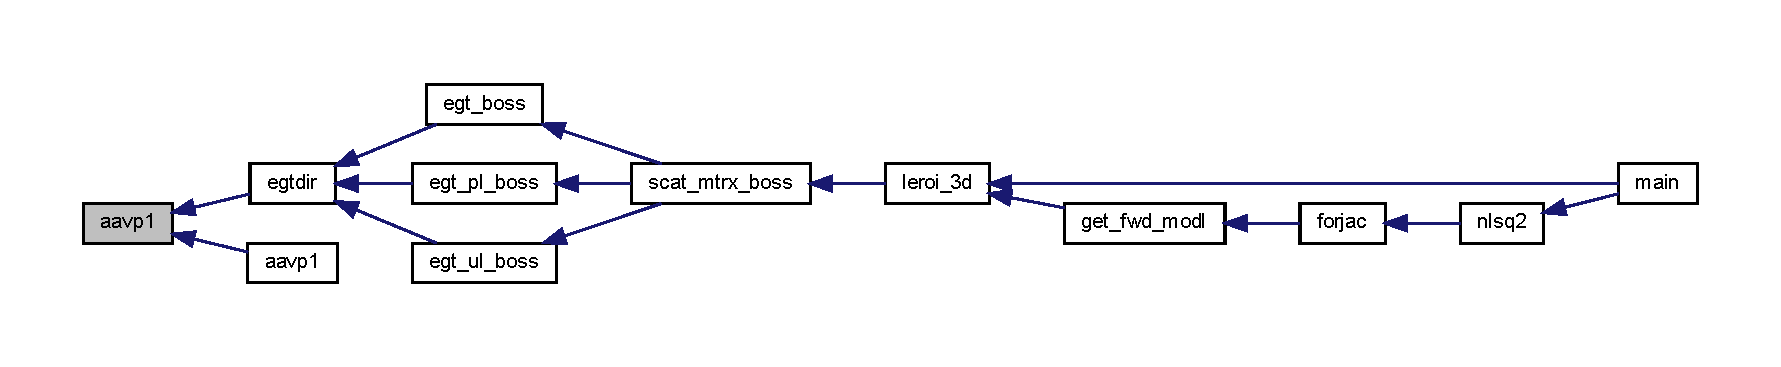
\includegraphics[width=350pt]{Leroi_8f90_a2d69cada9a1fff81caa02d919be5ce7c_icgraph}
\end{center}
\end{figure}
\mbox{\Hypertarget{Leroi_8f90_afeabf8ee47c9628f00ed2dfa98f56e40}\label{Leroi_8f90_afeabf8ee47c9628f00ed2dfa98f56e40}} 
\index{Leroi.\+f90@{Leroi.\+f90}!aavp2@{aavp2}}
\index{aavp2@{aavp2}!Leroi.\+f90@{Leroi.\+f90}}
\subsubsection{\texorpdfstring{aavp2()}{aavp2()}}
{\footnotesize\ttfamily complex function egtdir\+::aavp2 (\begin{DoxyParamCaption}\item[{complex}]{K\+B\+A\+SE,  }\item[{real}]{X1,  }\item[{real}]{Z1 }\end{DoxyParamCaption})}

Here is the caller graph for this function\+:\nopagebreak
\begin{figure}[H]
\begin{center}
\leavevmode
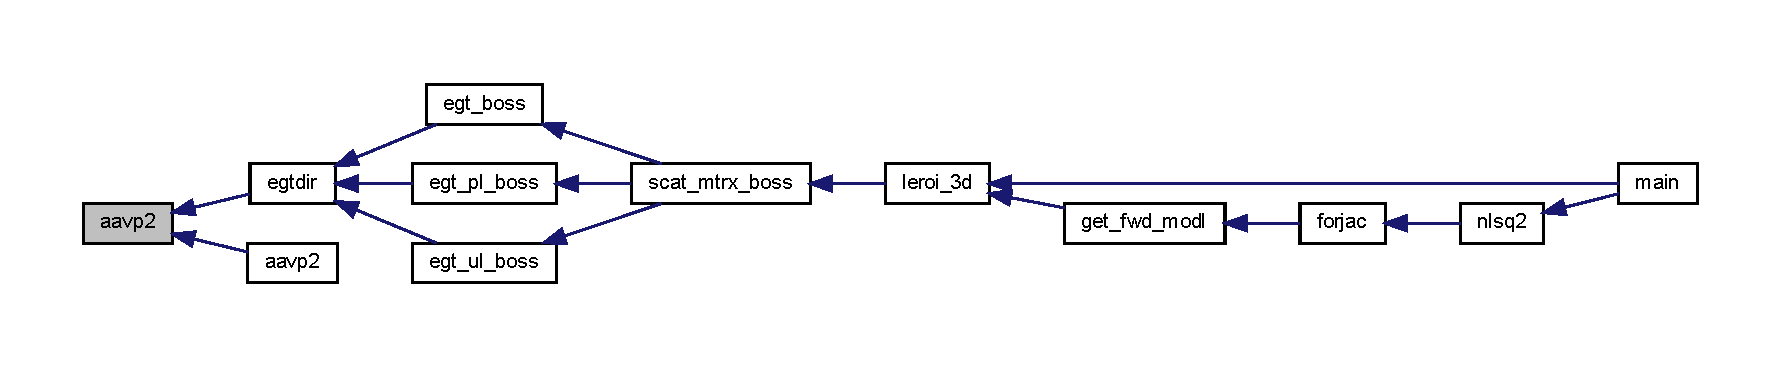
\includegraphics[width=350pt]{Leroi_8f90_afeabf8ee47c9628f00ed2dfa98f56e40_icgraph}
\end{center}
\end{figure}
\mbox{\Hypertarget{Leroi_8f90_a485defa6db785c79bb6a092cd797ca0e}\label{Leroi_8f90_a485defa6db785c79bb6a092cd797ca0e}} 
\index{Leroi.\+f90@{Leroi.\+f90}!b\+\_\+direct@{b\+\_\+direct}}
\index{b\+\_\+direct@{b\+\_\+direct}!Leroi.\+f90@{Leroi.\+f90}}
\subsubsection{\texorpdfstring{b\+\_\+direct()}{b\_direct()}}
{\footnotesize\ttfamily subroutine hsmdb\+::b\+\_\+direct (\begin{DoxyParamCaption}{ }\end{DoxyParamCaption})}

Here is the caller graph for this function\+:\nopagebreak
\begin{figure}[H]
\begin{center}
\leavevmode
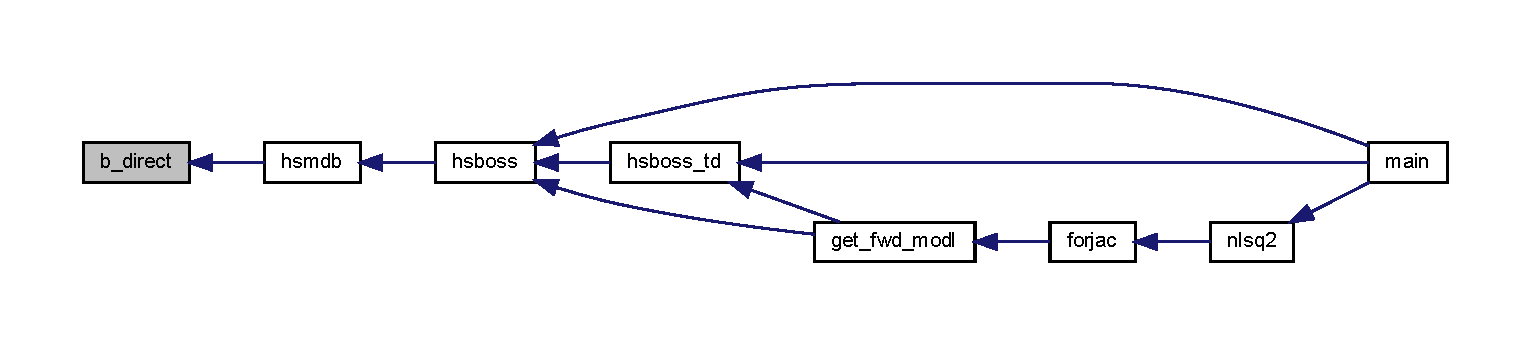
\includegraphics[width=350pt]{Leroi_8f90_a485defa6db785c79bb6a092cd797ca0e_icgraph}
\end{center}
\end{figure}
\mbox{\Hypertarget{Leroi_8f90_ab444c66af8ac23d415864bbbd3ff9872}\label{Leroi_8f90_ab444c66af8ac23d415864bbbd3ff9872}} 
\index{Leroi.\+f90@{Leroi.\+f90}!c2dintrp@{c2dintrp}}
\index{c2dintrp@{c2dintrp}!Leroi.\+f90@{Leroi.\+f90}}
\subsubsection{\texorpdfstring{c2dintrp()}{c2dintrp()}}
{\footnotesize\ttfamily complex function c2dintrp (\begin{DoxyParamCaption}\item[{real, dimension(nx)}]{XV,  }\item[{integer}]{NX,  }\item[{real, dimension(nz)}]{ZV,  }\item[{integer}]{NZ,  }\item[{real, dimension(4,nx,nz)}]{FR,  }\item[{real, dimension(4,nx,nz)}]{FI,  }\item[{real}]{X1,  }\item[{real}]{Z1 }\end{DoxyParamCaption})}

Here is the call graph for this function\+:\nopagebreak
\begin{figure}[H]
\begin{center}
\leavevmode
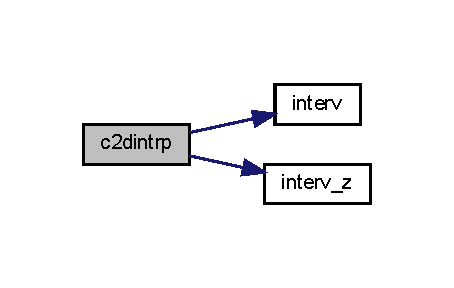
\includegraphics[width=218pt]{Leroi_8f90_ab444c66af8ac23d415864bbbd3ff9872_cgraph}
\end{center}
\end{figure}
Here is the caller graph for this function\+:\nopagebreak
\begin{figure}[H]
\begin{center}
\leavevmode
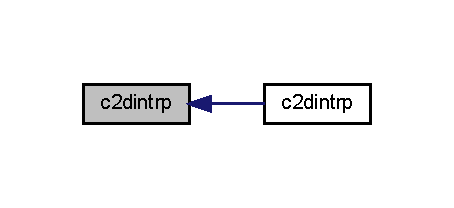
\includegraphics[width=218pt]{Leroi_8f90_ab444c66af8ac23d415864bbbd3ff9872_icgraph}
\end{center}
\end{figure}
\mbox{\Hypertarget{Leroi_8f90_a5a4be24a4461d42dc9be5d5388c4d366}\label{Leroi_8f90_a5a4be24a4461d42dc9be5d5388c4d366}} 
\index{Leroi.\+f90@{Leroi.\+f90}!ccubval@{ccubval}}
\index{ccubval@{ccubval}!Leroi.\+f90@{Leroi.\+f90}}
\subsubsection{\texorpdfstring{ccubval()}{ccubval()}}
{\footnotesize\ttfamily subroutine ccubval (\begin{DoxyParamCaption}\item[{real, dimension(nval)}]{X\+\_\+\+A\+R\+R\+AY,  }\item[{integer}]{N\+V\+AL,  }\item[{real, dimension(4,nval)}]{F\+U\+N\+\_\+R,  }\item[{real, dimension(4,nval)}]{F\+U\+N\+\_\+I,  }\item[{real}]{X1,  }\item[{complex}]{C2 }\end{DoxyParamCaption})}

Here is the call graph for this function\+:\nopagebreak
\begin{figure}[H]
\begin{center}
\leavevmode
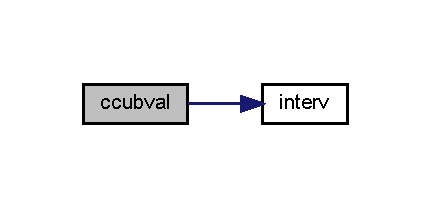
\includegraphics[width=207pt]{Leroi_8f90_a5a4be24a4461d42dc9be5d5388c4d366_cgraph}
\end{center}
\end{figure}
Here is the caller graph for this function\+:\nopagebreak
\begin{figure}[H]
\begin{center}
\leavevmode
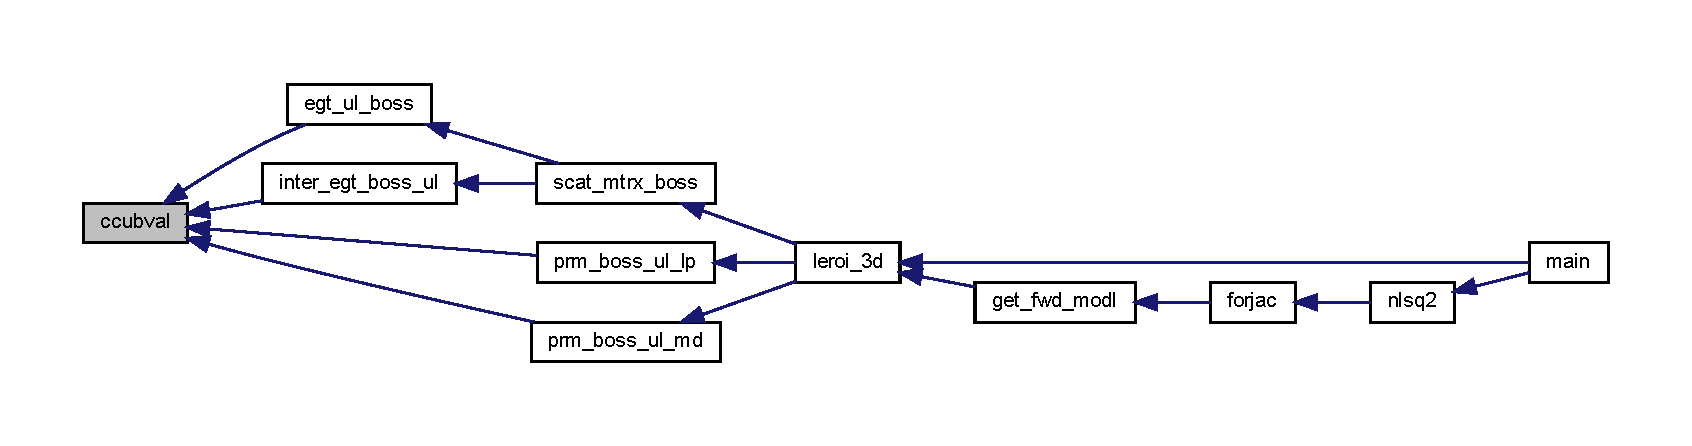
\includegraphics[width=350pt]{Leroi_8f90_a5a4be24a4461d42dc9be5d5388c4d366_icgraph}
\end{center}
\end{figure}
\mbox{\Hypertarget{Leroi_8f90_ab28d8a79c971f683b68fae4db0553909}\label{Leroi_8f90_ab28d8a79c971f683b68fae4db0553909}} 
\index{Leroi.\+f90@{Leroi.\+f90}!cdcubval@{cdcubval}}
\index{cdcubval@{cdcubval}!Leroi.\+f90@{Leroi.\+f90}}
\subsubsection{\texorpdfstring{cdcubval()}{cdcubval()}}
{\footnotesize\ttfamily subroutine cdcubval (\begin{DoxyParamCaption}\item[{real, dimension(nval)}]{X\+\_\+\+A\+R\+R\+AY,  }\item[{real, dimension(4,nval)}]{F\+U\+N\+\_\+R,  }\item[{real, dimension(4,nval)}]{F\+U\+N\+\_\+I,  }\item[{integer}]{N\+V\+AL,  }\item[{real(kind=ql)}]{X1,  }\item[{complex(kind=ql)}]{C\+D2 }\end{DoxyParamCaption})}

Here is the call graph for this function\+:\nopagebreak
\begin{figure}[H]
\begin{center}
\leavevmode
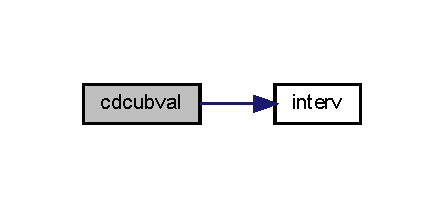
\includegraphics[width=213pt]{Leroi_8f90_ab28d8a79c971f683b68fae4db0553909_cgraph}
\end{center}
\end{figure}
Here is the caller graph for this function\+:\nopagebreak
\begin{figure}[H]
\begin{center}
\leavevmode
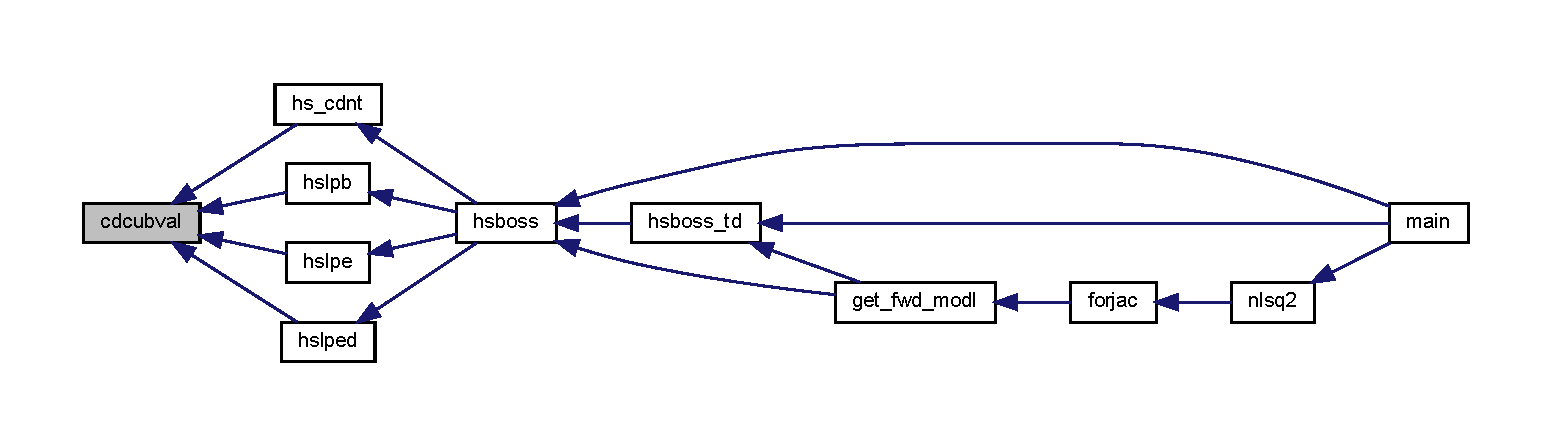
\includegraphics[width=350pt]{Leroi_8f90_ab28d8a79c971f683b68fae4db0553909_icgraph}
\end{center}
\end{figure}
\mbox{\Hypertarget{Leroi_8f90_a747a5bf7d69f6533bc2f54572584ba0c}\label{Leroi_8f90_a747a5bf7d69f6533bc2f54572584ba0c}} 
\index{Leroi.\+f90@{Leroi.\+f90}!cnvrt2\+\_\+mpar@{cnvrt2\+\_\+mpar}}
\index{cnvrt2\+\_\+mpar@{cnvrt2\+\_\+mpar}!Leroi.\+f90@{Leroi.\+f90}}
\subsubsection{\texorpdfstring{cnvrt2\+\_\+mpar()}{cnvrt2\_mpar()}}
{\footnotesize\ttfamily subroutine cnvrt2\+\_\+mpar (\begin{DoxyParamCaption}\item[{integer}]{N\+L\+YR,  }\item[{integer}]{N\+P\+LT,  }\item[{integer}]{N\+P\+AR,  }\item[{real, dimension(nlyr)}]{R\+ES,  }\item[{real, dimension(nlyr)}]{T\+HK,  }\item[{real, dimension(nplt)}]{S\+I\+G\+\_\+T,  }\item[{real, dimension(nplt)}]{P\+L\+T\+OP,  }\item[{real, dimension(nplt)}]{P\+L\+N\+G\+TH,  }\item[{real, dimension(nplt)}]{P\+L\+W\+D\+TH,  }\item[{real, dimension(nplt)}]{X\+C\+N\+TR,  }\item[{real, dimension(nplt)}]{Y\+C\+N\+TR,  }\item[{real, dimension(nplt)}]{X\+Y\+N\+O\+RM,  }\item[{real, dimension(nplt)}]{P\+L\+A\+ZM,  }\item[{real, dimension(nplt)}]{P\+L\+D\+IP,  }\item[{real, dimension(nplt)}]{P\+L\+U\+NJ,  }\item[{real, dimension(npar)}]{X\+P\+AR }\end{DoxyParamCaption})}

Here is the caller graph for this function\+:\nopagebreak
\begin{figure}[H]
\begin{center}
\leavevmode
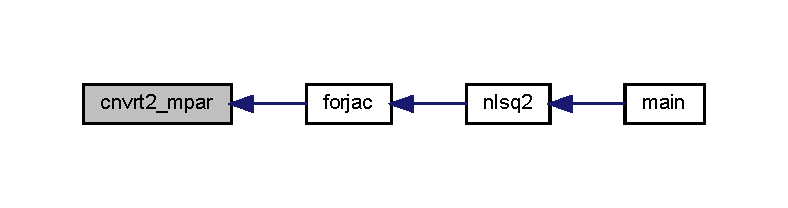
\includegraphics[width=350pt]{Leroi_8f90_a747a5bf7d69f6533bc2f54572584ba0c_icgraph}
\end{center}
\end{figure}
\mbox{\Hypertarget{Leroi_8f90_aa8246fcc58fb68567634de3315aa33d2}\label{Leroi_8f90_aa8246fcc58fb68567634de3315aa33d2}} 
\index{Leroi.\+f90@{Leroi.\+f90}!cnvrt2\+\_\+xpar@{cnvrt2\+\_\+xpar}}
\index{cnvrt2\+\_\+xpar@{cnvrt2\+\_\+xpar}!Leroi.\+f90@{Leroi.\+f90}}
\subsubsection{\texorpdfstring{cnvrt2\+\_\+xpar()}{cnvrt2\_xpar()}}
{\footnotesize\ttfamily subroutine cnvrt2\+\_\+xpar (\begin{DoxyParamCaption}\item[{integer}]{N\+L\+YR,  }\item[{integer}]{N\+P\+LT,  }\item[{integer}]{N\+P\+AR,  }\item[{real, dimension(nlyr)}]{R\+ES,  }\item[{real, dimension(nlyr)}]{T\+HK,  }\item[{real, dimension(nplt)}]{S\+I\+G\+\_\+T,  }\item[{real, dimension(nplt)}]{P\+L\+T\+OP,  }\item[{real, dimension(nplt)}]{P\+L\+N\+G\+TH,  }\item[{real, dimension(nplt)}]{P\+L\+W\+D\+TH,  }\item[{real, dimension(nplt)}]{X\+C\+N\+TR,  }\item[{real, dimension(nplt)}]{Y\+C\+N\+TR,  }\item[{real, dimension(nplt)}]{X\+Y\+N\+O\+RM,  }\item[{real, dimension(nplt)}]{P\+L\+A\+ZM,  }\item[{real, dimension(nplt)}]{P\+L\+D\+IP,  }\item[{real, dimension(nplt)}]{P\+L\+U\+NJ,  }\item[{real, dimension(npar)}]{X\+P\+AR }\end{DoxyParamCaption})}

Here is the caller graph for this function\+:\nopagebreak
\begin{figure}[H]
\begin{center}
\leavevmode
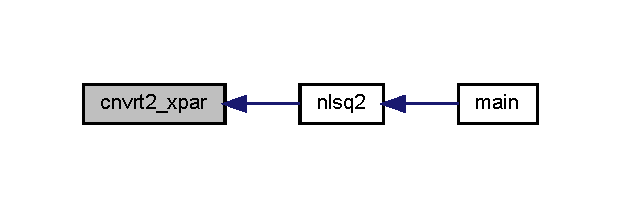
\includegraphics[width=298pt]{Leroi_8f90_aa8246fcc58fb68567634de3315aa33d2_icgraph}
\end{center}
\end{figure}
\mbox{\Hypertarget{Leroi_8f90_a0801b4ca30057cb8ddfb94e49185a2ce}\label{Leroi_8f90_a0801b4ca30057cb8ddfb94e49185a2ce}} 
\index{Leroi.\+f90@{Leroi.\+f90}!cnvrt\+\_\+bounds@{cnvrt\+\_\+bounds}}
\index{cnvrt\+\_\+bounds@{cnvrt\+\_\+bounds}!Leroi.\+f90@{Leroi.\+f90}}
\subsubsection{\texorpdfstring{cnvrt\+\_\+bounds()}{cnvrt\_bounds()}}
{\footnotesize\ttfamily subroutine cnvrt\+\_\+bounds (\begin{DoxyParamCaption}\item[{integer}]{N\+P\+LT,  }\item[{integer}]{N\+L\+YR,  }\item[{integer}]{N\+P\+AR,  }\item[{real, dimension(npar)}]{L\+B\+ND,  }\item[{real, dimension(npar)}]{U\+B\+ND,  }\item[{real, dimension(nplt)}]{X\+Y\+N\+O\+RM,  }\item[{integer, dimension(npar)}]{C\+X\+P\+AR,  }\item[{real, dimension(npar)}]{X\+L\+B\+ND,  }\item[{real, dimension(npar)}]{X\+U\+B\+ND }\end{DoxyParamCaption})}

Here is the caller graph for this function\+:\nopagebreak
\begin{figure}[H]
\begin{center}
\leavevmode
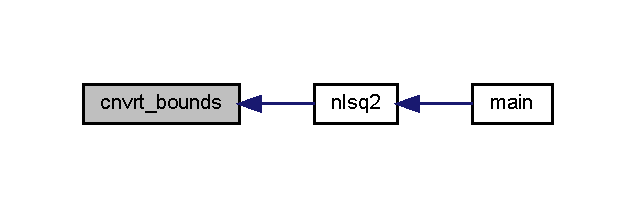
\includegraphics[width=305pt]{Leroi_8f90_a0801b4ca30057cb8ddfb94e49185a2ce_icgraph}
\end{center}
\end{figure}
\mbox{\Hypertarget{Leroi_8f90_a36d9dbba0b5eada45705f561c0035c54}\label{Leroi_8f90_a36d9dbba0b5eada45705f561c0035c54}} 
\index{Leroi.\+f90@{Leroi.\+f90}!colres\+\_\+1d@{colres\+\_\+1d}}
\index{colres\+\_\+1d@{colres\+\_\+1d}!Leroi.\+f90@{Leroi.\+f90}}
\subsubsection{\texorpdfstring{colres\+\_\+1d()}{colres\_1d()}}
{\footnotesize\ttfamily subroutine colres\+\_\+1d (\begin{DoxyParamCaption}\item[{real}]{F\+RQ,  }\item[{integer}]{N\+L\+YR,  }\item[{real, dimension(nlyr)}]{R\+ES,  }\item[{real, dimension(nlyr)}]{R\+E\+PS,  }\item[{real(kind=ql), dimension(0\+:nlyr)}]{R\+M\+UD,  }\item[{real, dimension(nlyr)}]{C\+H\+RG,  }\item[{real, dimension(nlyr)}]{C\+T\+AU,  }\item[{real, dimension(nlyr)}]{C\+F\+R\+EQ,  }\item[{complex(kind=ql), dimension (nlyr)}]{S\+I\+GL,  }\item[{complex(kind=ql), dimension (nlyr)}]{K\+S\+QL }\end{DoxyParamCaption})}

Here is the caller graph for this function\+:\nopagebreak
\begin{figure}[H]
\begin{center}
\leavevmode
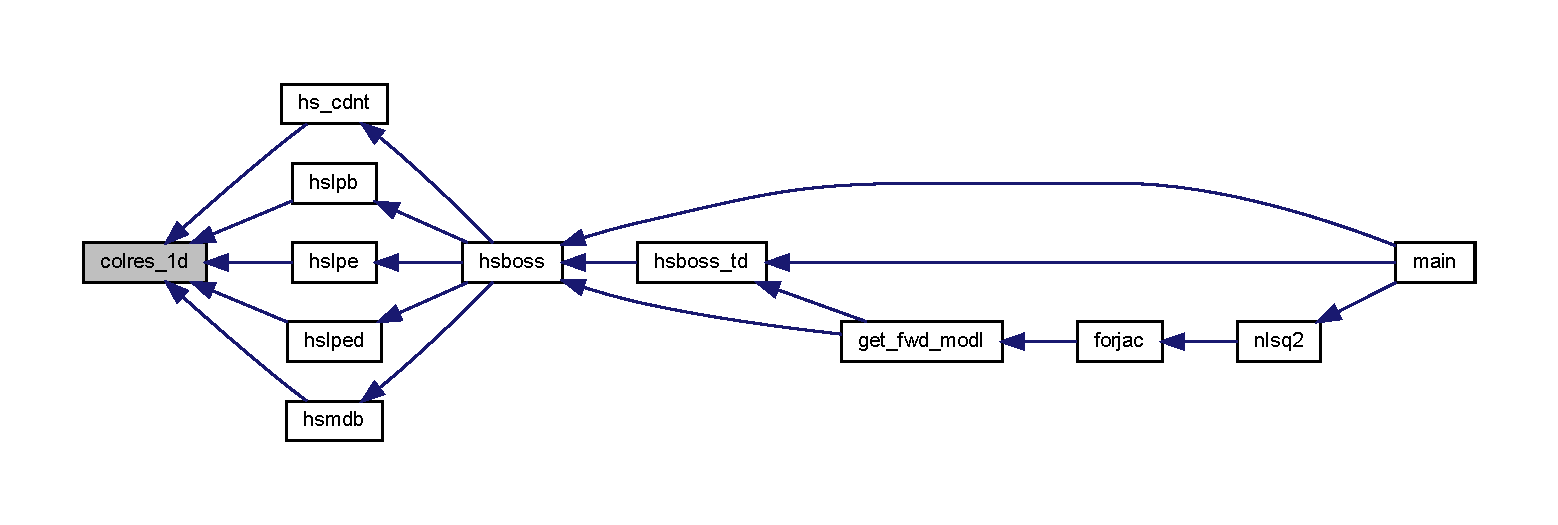
\includegraphics[width=350pt]{Leroi_8f90_a36d9dbba0b5eada45705f561c0035c54_icgraph}
\end{center}
\end{figure}
\mbox{\Hypertarget{Leroi_8f90_a61eed94d3789d0474014a2cd34a792c6}\label{Leroi_8f90_a61eed94d3789d0474014a2cd34a792c6}} 
\index{Leroi.\+f90@{Leroi.\+f90}!colres\+\_\+3d@{colres\+\_\+3d}}
\index{colres\+\_\+3d@{colres\+\_\+3d}!Leroi.\+f90@{Leroi.\+f90}}
\subsubsection{\texorpdfstring{colres\+\_\+3d()}{colres\_3d()}}
{\footnotesize\ttfamily subroutine colres\+\_\+3d (\begin{DoxyParamCaption}\item[{real}]{F\+RQ,  }\item[{integer}]{N\+L\+YR,  }\item[{real(kind=ql), dimension(0\+:nlyr)}]{R\+M\+UD,  }\item[{real, dimension(nlyr)}]{R\+ES,  }\item[{real, dimension(nlyr)}]{R\+E\+PS,  }\item[{integer, dimension(nlyr)}]{I\+C\+CL,  }\item[{real, dimension(nlyr)}]{C\+H\+RG,  }\item[{real, dimension(nlyr)}]{C\+T\+AU,  }\item[{real, dimension(nlyr)}]{C\+F\+R\+EQ,  }\item[{integer}]{N\+P\+LT,  }\item[{real, dimension(nplt)}]{S\+I\+G\+\_\+T,  }\item[{real, dimension(nplt)}]{C\+H\+R\+GP,  }\item[{real, dimension(nplt)}]{C\+T\+A\+UP,  }\item[{real, dimension(nplt)}]{C\+F\+R\+E\+QP,  }\item[{integer, dimension(nplt)}]{I\+C\+CP,  }\item[{complex(kind=ql), dimension(nlyr)}]{S\+I\+GL,  }\item[{complex(kind=ql), dimension(nlyr)}]{K\+S\+QL,  }\item[{complex, dimension(nplt)}]{S\+I\+GT,  }\item[{complex, dimension(nplt)}]{K\+S\+QT }\end{DoxyParamCaption})}

Here is the caller graph for this function\+:\nopagebreak
\begin{figure}[H]
\begin{center}
\leavevmode
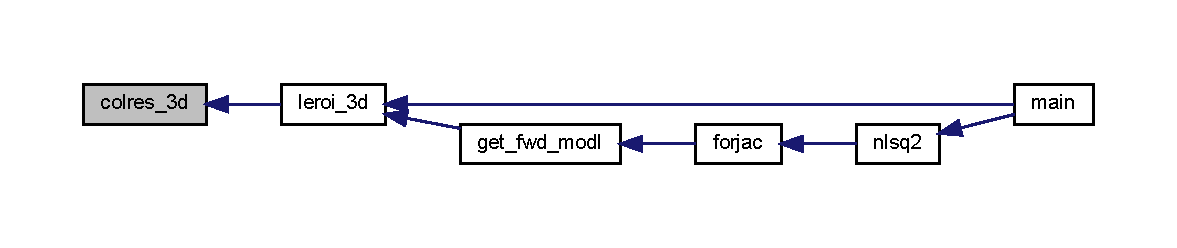
\includegraphics[width=350pt]{Leroi_8f90_a61eed94d3789d0474014a2cd34a792c6_icgraph}
\end{center}
\end{figure}
\mbox{\Hypertarget{Leroi_8f90_a12a40dde1170214455093566ef5e8bb4}\label{Leroi_8f90_a12a40dde1170214455093566ef5e8bb4}} 
\index{Leroi.\+f90@{Leroi.\+f90}!costrn@{costrn}}
\index{costrn@{costrn}!Leroi.\+f90@{Leroi.\+f90}}
\subsubsection{\texorpdfstring{costrn()}{costrn()}}
{\footnotesize\ttfamily real function costrn (\begin{DoxyParamCaption}\item[{real, dimension(nfrq), intent(in)}]{WF,  }\item[{real, dimension(4,nfrq), intent(in)}]{Y\+F\+RQ,  }\item[{integer, intent(in)}]{N\+F\+RQ,  }\item[{real, intent(in)}]{T }\end{DoxyParamCaption})}

Here is the caller graph for this function\+:\nopagebreak
\begin{figure}[H]
\begin{center}
\leavevmode
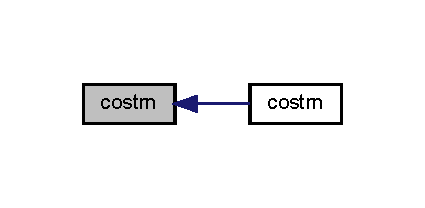
\includegraphics[width=204pt]{Leroi_8f90_a12a40dde1170214455093566ef5e8bb4_icgraph}
\end{center}
\end{figure}
\mbox{\Hypertarget{Leroi_8f90_aee021b0986763ff84e2a9373cd2c5b9f}\label{Leroi_8f90_aee021b0986763ff84e2a9373cd2c5b9f}} 
\index{Leroi.\+f90@{Leroi.\+f90}!cubint@{cubint}}
\index{cubint@{cubint}!Leroi.\+f90@{Leroi.\+f90}}
\subsubsection{\texorpdfstring{cubint()}{cubint()}}
{\footnotesize\ttfamily real function cubint (\begin{DoxyParamCaption}\item[{real, dimension(nval)}]{X\+\_\+\+A\+R\+R\+AY,  }\item[{real, dimension(4,nval)}]{Y\+\_\+\+V\+AL,  }\item[{integer}]{N\+V\+AL,  }\item[{real}]{X1,  }\item[{real}]{X2 }\end{DoxyParamCaption})}

Here is the call graph for this function\+:\nopagebreak
\begin{figure}[H]
\begin{center}
\leavevmode
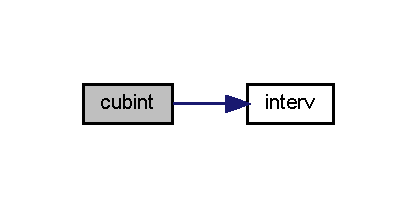
\includegraphics[width=200pt]{Leroi_8f90_aee021b0986763ff84e2a9373cd2c5b9f_cgraph}
\end{center}
\end{figure}
Here is the caller graph for this function\+:\nopagebreak
\begin{figure}[H]
\begin{center}
\leavevmode
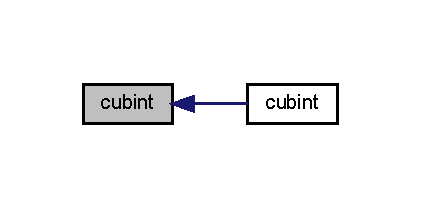
\includegraphics[width=202pt]{Leroi_8f90_aee021b0986763ff84e2a9373cd2c5b9f_icgraph}
\end{center}
\end{figure}
\mbox{\Hypertarget{Leroi_8f90_a836d1cb8acb3544a3a9fa63433efc1b6}\label{Leroi_8f90_a836d1cb8acb3544a3a9fa63433efc1b6}} 
\index{Leroi.\+f90@{Leroi.\+f90}!cubspl@{cubspl}}
\index{cubspl@{cubspl}!Leroi.\+f90@{Leroi.\+f90}}
\subsubsection{\texorpdfstring{cubspl()}{cubspl()}}
{\footnotesize\ttfamily subroutine cubspl (\begin{DoxyParamCaption}\item[{real, dimension(n)}]{X\+V\+AL,  }\item[{real, dimension(4,n)}]{F,  }\item[{integer}]{N }\end{DoxyParamCaption})}

Here is the caller graph for this function\+:\nopagebreak
\begin{figure}[H]
\begin{center}
\leavevmode
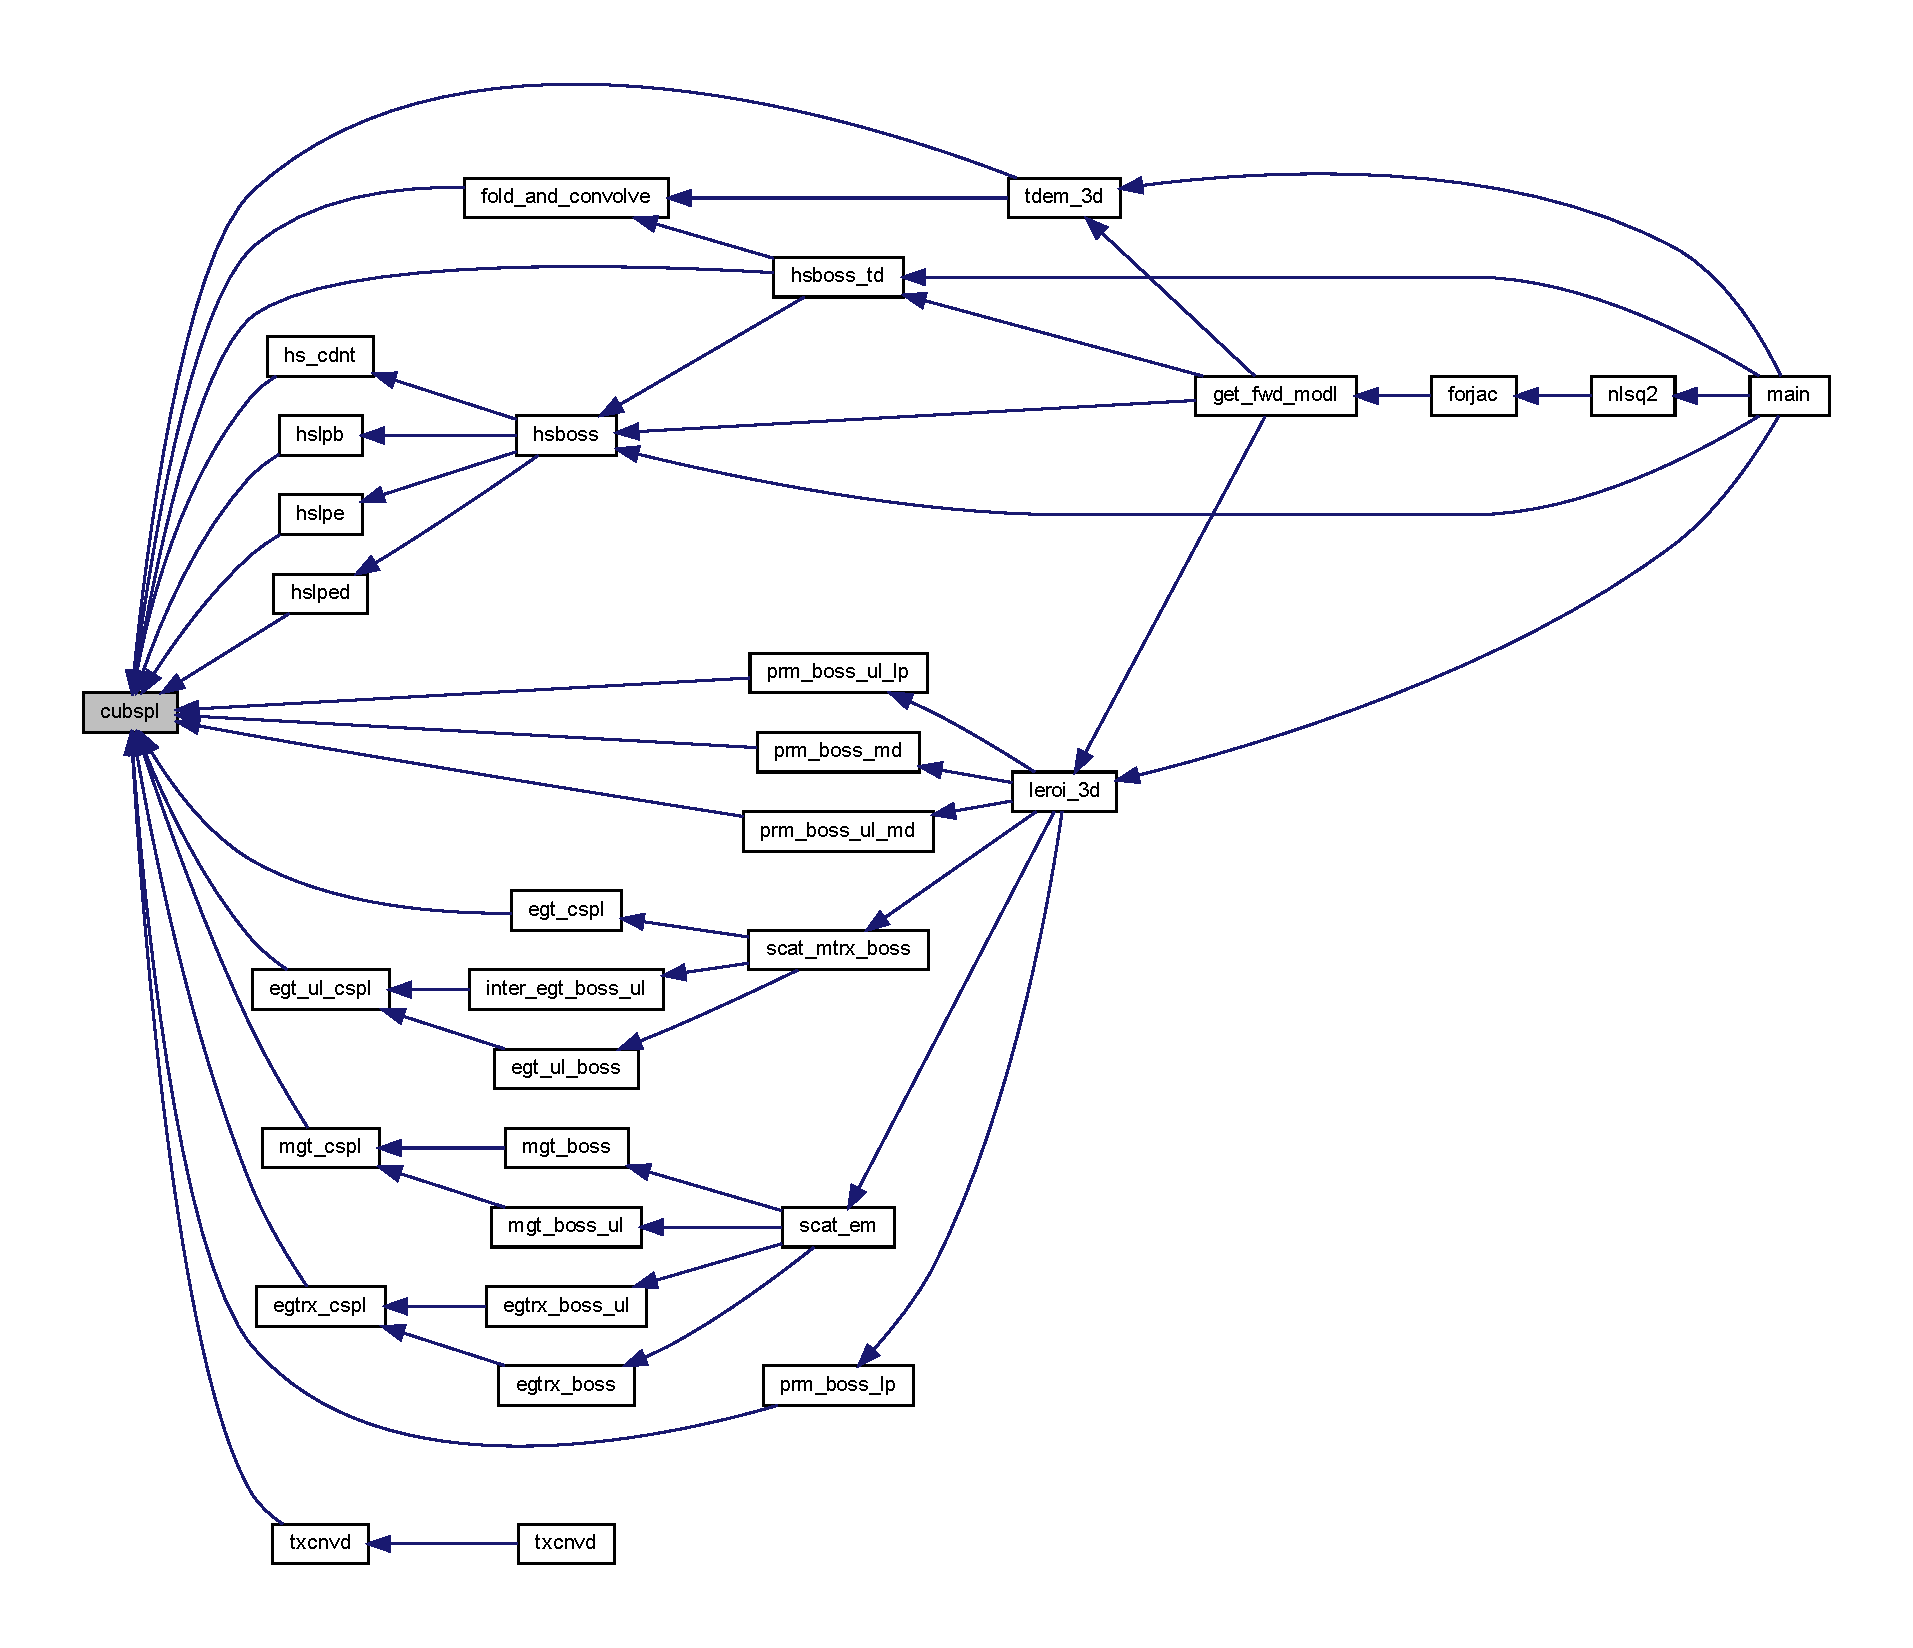
\includegraphics[width=350pt]{Leroi_8f90_a836d1cb8acb3544a3a9fa63433efc1b6_icgraph}
\end{center}
\end{figure}
\mbox{\Hypertarget{Leroi_8f90_a7cfee47c046d9dadca7ccd1059bd30ac}\label{Leroi_8f90_a7cfee47c046d9dadca7ccd1059bd30ac}} 
\index{Leroi.\+f90@{Leroi.\+f90}!cubval@{cubval}}
\index{cubval@{cubval}!Leroi.\+f90@{Leroi.\+f90}}
\subsubsection{\texorpdfstring{cubval()}{cubval()}}
{\footnotesize\ttfamily real function cubval (\begin{DoxyParamCaption}\item[{real, dimension(nxval), intent(in)}]{X\+\_\+\+A\+R\+R\+AY,  }\item[{real, dimension(4,nxval), intent(in)}]{Y\+\_\+\+V\+AL,  }\item[{integer, intent(in)}]{N\+X\+V\+AL,  }\item[{real, intent(in)}]{X1 }\end{DoxyParamCaption})}

Here is the call graph for this function\+:\nopagebreak
\begin{figure}[H]
\begin{center}
\leavevmode
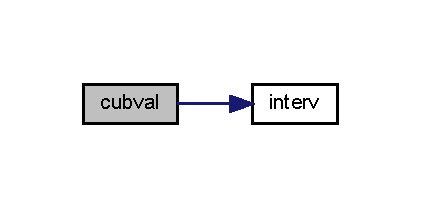
\includegraphics[width=202pt]{Leroi_8f90_a7cfee47c046d9dadca7ccd1059bd30ac_cgraph}
\end{center}
\end{figure}
Here is the caller graph for this function\+:\nopagebreak
\begin{figure}[H]
\begin{center}
\leavevmode
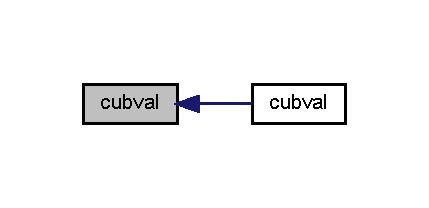
\includegraphics[width=206pt]{Leroi_8f90_a7cfee47c046d9dadca7ccd1059bd30ac_icgraph}
\end{center}
\end{figure}
\mbox{\Hypertarget{Leroi_8f90_a7ac3bb5f2b2d31402aa81424ee2be857}\label{Leroi_8f90_a7ac3bb5f2b2d31402aa81424ee2be857}} 
\index{Leroi.\+f90@{Leroi.\+f90}!cubvalrz@{cubvalrz}}
\index{cubvalrz@{cubvalrz}!Leroi.\+f90@{Leroi.\+f90}}
\subsubsection{\texorpdfstring{cubvalrz()}{cubvalrz()}}
{\footnotesize\ttfamily subroutine cubvalrz (\begin{DoxyParamCaption}\item[{real, dimension(nrval)}]{X\+\_\+\+A\+R\+R\+AY,  }\item[{integer}]{N\+R\+V\+AL,  }\item[{integer}]{N\+Z\+V\+AL,  }\item[{real, dimension(4,nrval,nzval)}]{F\+U\+N\+\_\+R,  }\item[{real, dimension(4,nrval,nzval)}]{F\+U\+N\+\_\+I,  }\item[{real}]{X1,  }\item[{integer}]{JZ,  }\item[{complex}]{C2 }\end{DoxyParamCaption})}

Here is the call graph for this function\+:\nopagebreak
\begin{figure}[H]
\begin{center}
\leavevmode
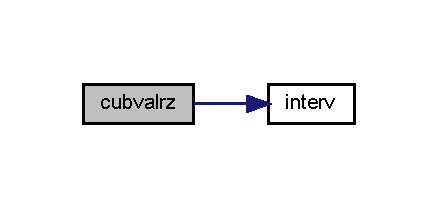
\includegraphics[width=210pt]{Leroi_8f90_a7ac3bb5f2b2d31402aa81424ee2be857_cgraph}
\end{center}
\end{figure}
Here is the caller graph for this function\+:\nopagebreak
\begin{figure}[H]
\begin{center}
\leavevmode
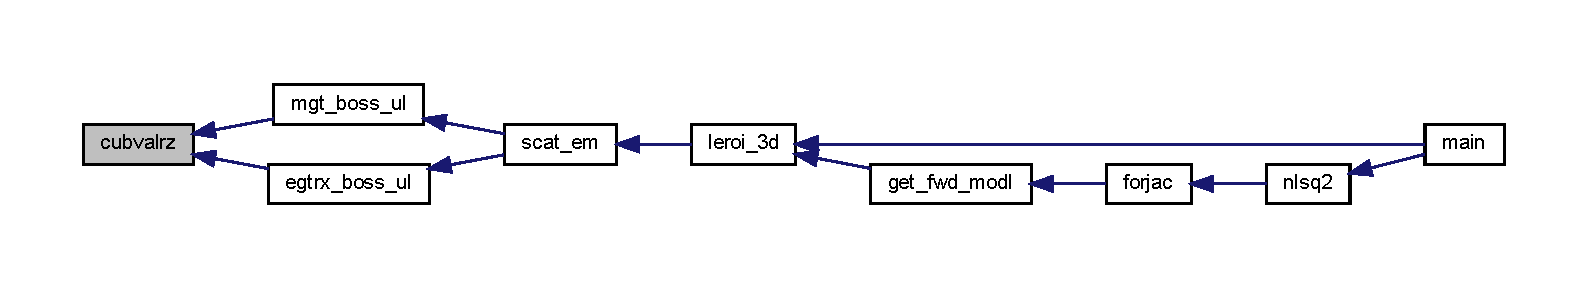
\includegraphics[width=350pt]{Leroi_8f90_a7ac3bb5f2b2d31402aa81424ee2be857_icgraph}
\end{center}
\end{figure}
\mbox{\Hypertarget{Leroi_8f90_a173fbca69518ee77703afb9c67d3e4f0}\label{Leroi_8f90_a173fbca69518ee77703afb9c67d3e4f0}} 
\index{Leroi.\+f90@{Leroi.\+f90}!dist2d@{dist2d}}
\index{dist2d@{dist2d}!Leroi.\+f90@{Leroi.\+f90}}
\subsubsection{\texorpdfstring{dist2d()}{dist2d()}}
{\footnotesize\ttfamily real function dist2d (\begin{DoxyParamCaption}\item[{real}]{X1,  }\item[{real}]{Y1,  }\item[{real}]{X2,  }\item[{real}]{Y2 }\end{DoxyParamCaption})}

Here is the caller graph for this function\+:\nopagebreak
\begin{figure}[H]
\begin{center}
\leavevmode
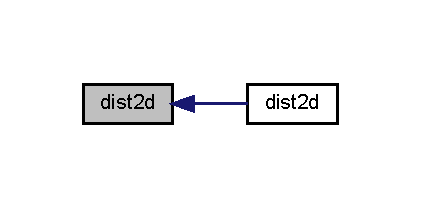
\includegraphics[width=202pt]{Leroi_8f90_a173fbca69518ee77703afb9c67d3e4f0_icgraph}
\end{center}
\end{figure}
\mbox{\Hypertarget{Leroi_8f90_a728fa0fc652b63cee1eb0d408bbac553}\label{Leroi_8f90_a728fa0fc652b63cee1eb0d408bbac553}} 
\index{Leroi.\+f90@{Leroi.\+f90}!dprod1@{dprod1}}
\index{dprod1@{dprod1}!Leroi.\+f90@{Leroi.\+f90}}
\subsubsection{\texorpdfstring{dprod1()}{dprod1()}}
{\footnotesize\ttfamily real function dprod1 (\begin{DoxyParamCaption}\item[{integer, intent(in)}]{N,  }\item[{integer, intent(in)}]{N1,  }\item[{integer, intent(in)}]{N2,  }\item[{real, intent(in)}]{A,  }\item[{real, dimension(1), intent(in)}]{B,  }\item[{real, dimension(1), intent(in)}]{C }\end{DoxyParamCaption})}

Here is the caller graph for this function\+:\nopagebreak
\begin{figure}[H]
\begin{center}
\leavevmode
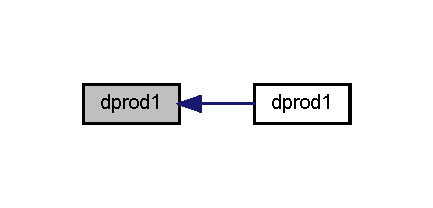
\includegraphics[width=208pt]{Leroi_8f90_a728fa0fc652b63cee1eb0d408bbac553_icgraph}
\end{center}
\end{figure}
\mbox{\Hypertarget{Leroi_8f90_a0dd58336077baa8c233cc4d08cc10939}\label{Leroi_8f90_a0dd58336077baa8c233cc4d08cc10939}} 
\index{Leroi.\+f90@{Leroi.\+f90}!dqdx@{dqdx}}
\index{dqdx@{dqdx}!Leroi.\+f90@{Leroi.\+f90}}
\subsubsection{\texorpdfstring{dqdx()}{dqdx()}}
{\footnotesize\ttfamily complex function egtdir\+::dqdx (\begin{DoxyParamCaption}\item[{complex}]{K\+B\+A\+SE,  }\item[{real}]{X1,  }\item[{real}]{Z1 }\end{DoxyParamCaption})}

Here is the caller graph for this function\+:\nopagebreak
\begin{figure}[H]
\begin{center}
\leavevmode
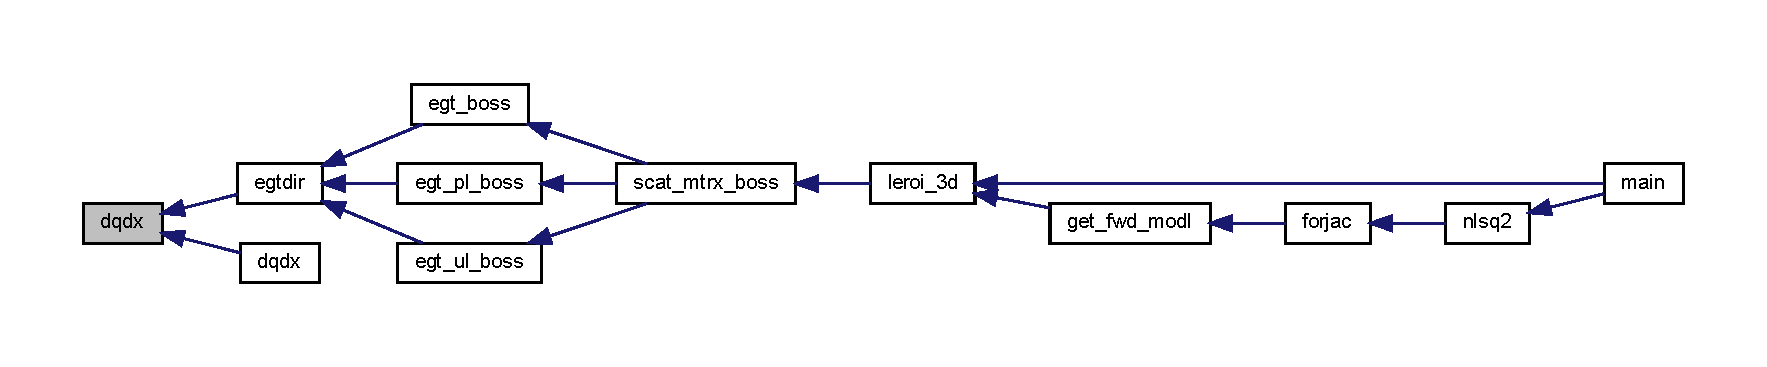
\includegraphics[width=350pt]{Leroi_8f90_a0dd58336077baa8c233cc4d08cc10939_icgraph}
\end{center}
\end{figure}
\mbox{\Hypertarget{Leroi_8f90_a2ffa10f72b064e2c52fb28da1b335098}\label{Leroi_8f90_a2ffa10f72b064e2c52fb28da1b335098}} 
\index{Leroi.\+f90@{Leroi.\+f90}!edsx\+\_\+coef@{edsx\+\_\+coef}}
\index{edsx\+\_\+coef@{edsx\+\_\+coef}!Leroi.\+f90@{Leroi.\+f90}}
\subsubsection{\texorpdfstring{edsx\+\_\+coef()}{edsx\_coef()}}
{\footnotesize\ttfamily subroutine edsx\+\_\+coef (\begin{DoxyParamCaption}\item[{integer}]{S\+X\+L\+YR,  }\item[{integer}]{R\+X\+L\+YR,  }\item[{integer}]{K\+FG,  }\item[{real(kind=ql)}]{L\+M\+B\+DA,  }\item[{integer}]{N\+L\+YR,  }\item[{real(kind=ql), dimension (nlyr)}]{T\+H\+KD,  }\item[{real(kind=ql), dimension (nlyr)}]{D\+P\+T\+HL,  }\item[{real(kind=ql), dimension(0\+:nlyr)}]{R\+M\+UD,  }\item[{complex(kind=ql), dimension (nlyr)}]{S\+I\+GL,  }\item[{complex(kind=ql), dimension (nlyr)}]{K\+S\+QL,  }\item[{real(kind=ql)}]{ZS,  }\item[{complex(kind=ql), dimension (0\+:nlyr)}]{S,  }\item[{complex(kind=ql)}]{X\+I\+\_\+V,  }\item[{complex(kind=ql)}]{F\+\_\+V,  }\item[{complex(kind=ql)}]{F\+\_\+H,  }\item[{complex(kind=ql)}]{E\+T\+A\+\_\+V,  }\item[{complex(kind=ql)}]{G\+\_\+V,  }\item[{complex(kind=ql)}]{G\+\_\+H }\end{DoxyParamCaption})}

Here is the call graph for this function\+:\nopagebreak
\begin{figure}[H]
\begin{center}
\leavevmode
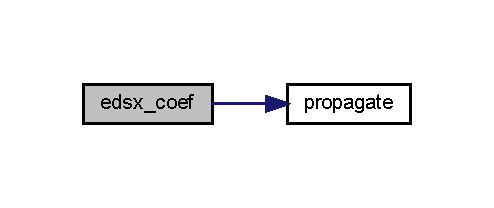
\includegraphics[width=237pt]{Leroi_8f90_a2ffa10f72b064e2c52fb28da1b335098_cgraph}
\end{center}
\end{figure}
Here is the caller graph for this function\+:\nopagebreak
\begin{figure}[H]
\begin{center}
\leavevmode
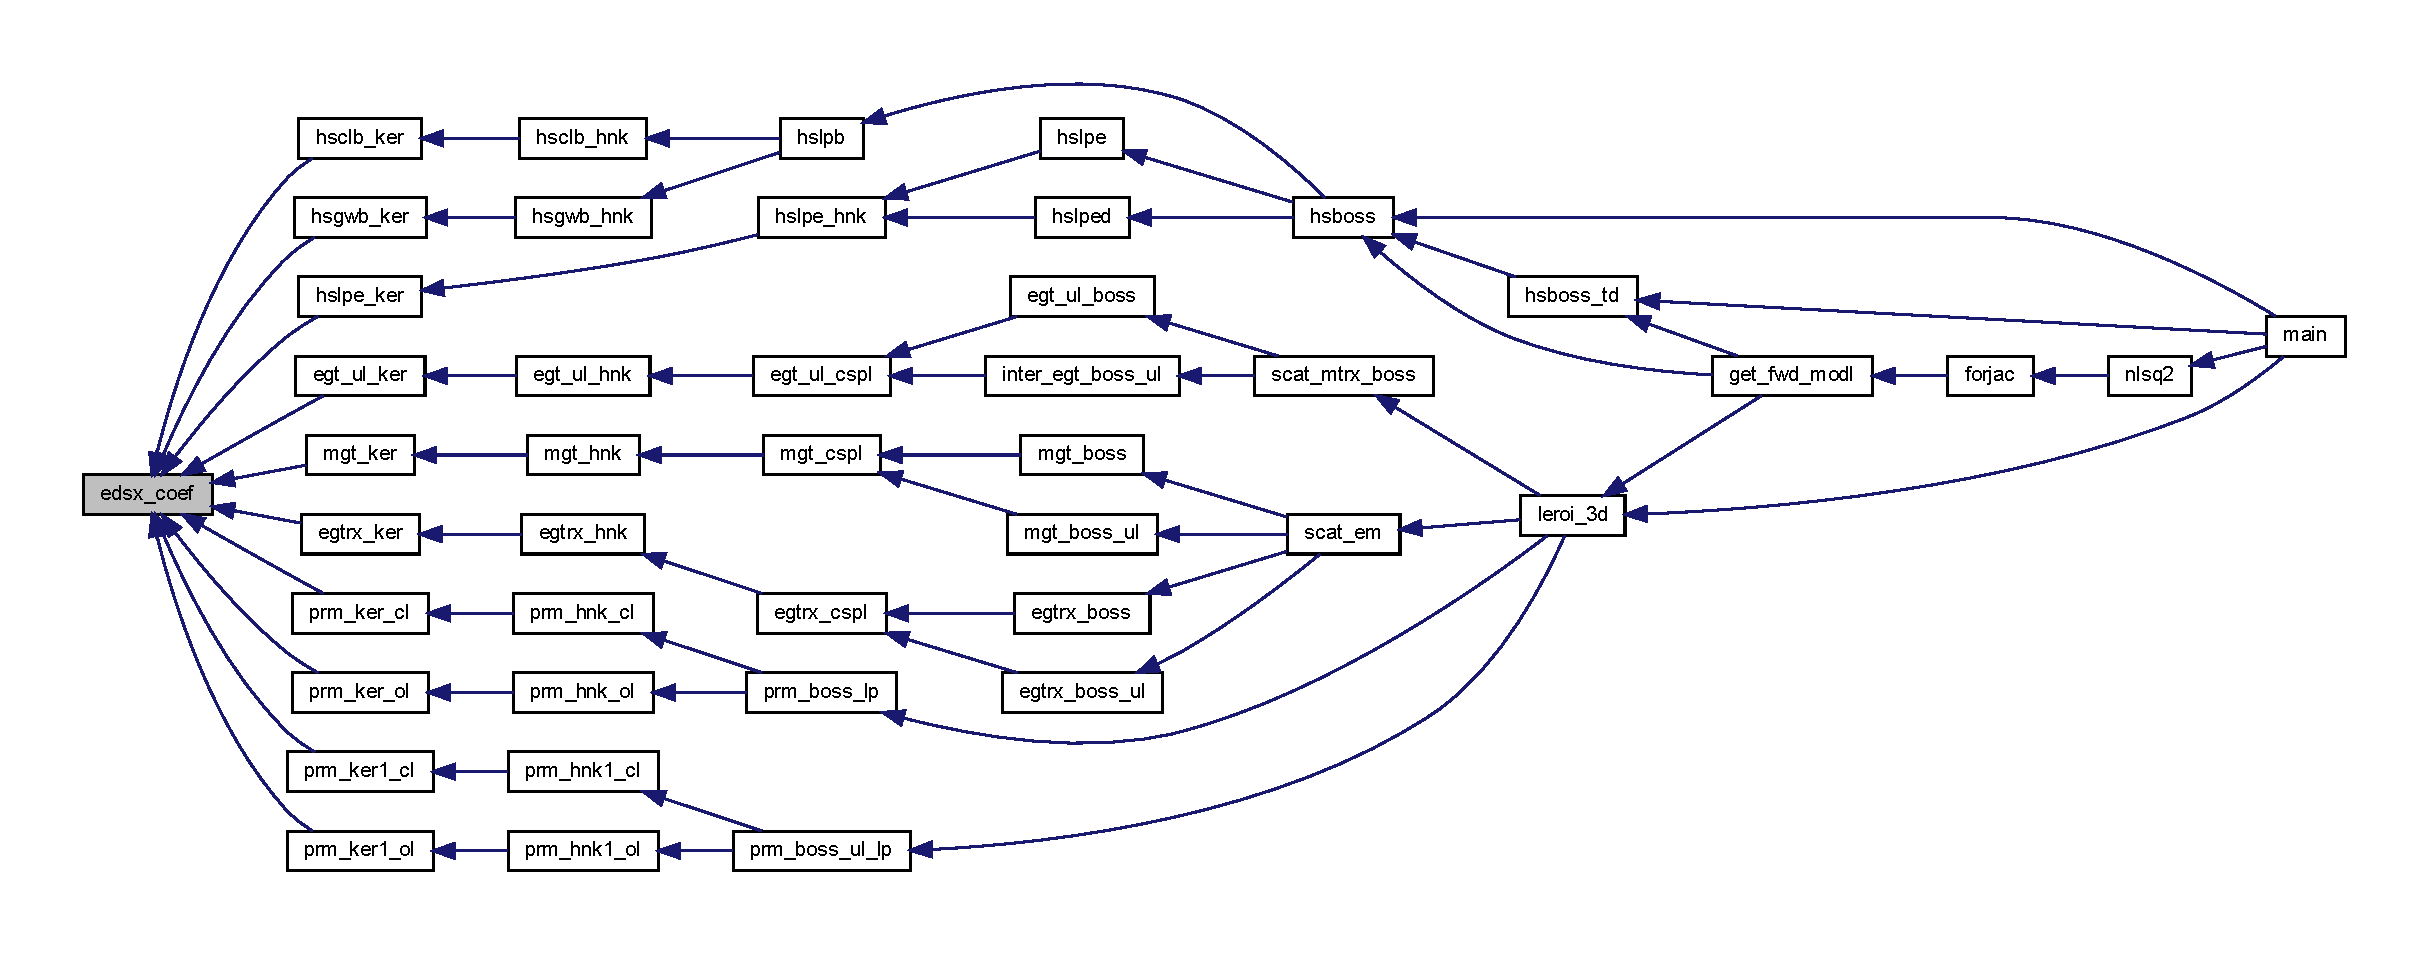
\includegraphics[width=350pt]{Leroi_8f90_a2ffa10f72b064e2c52fb28da1b335098_icgraph}
\end{center}
\end{figure}
\mbox{\Hypertarget{Leroi_8f90_a1b3954d66e2114dd2d6b6a5a44b7f0a4}\label{Leroi_8f90_a1b3954d66e2114dd2d6b6a5a44b7f0a4}} 
\index{Leroi.\+f90@{Leroi.\+f90}!egt\+\_\+boss@{egt\+\_\+boss}}
\index{egt\+\_\+boss@{egt\+\_\+boss}!Leroi.\+f90@{Leroi.\+f90}}
\subsubsection{\texorpdfstring{egt\+\_\+boss()}{egt\_boss()}}
{\footnotesize\ttfamily subroutine egt\+\_\+boss (\begin{DoxyParamCaption}\item[{integer}]{N\+AL,  }\item[{integer}]{N\+BL,  }\item[{integer}]{N\+AB,  }\item[{real}]{D\+AL,  }\item[{real}]{D\+BL,  }\item[{complex}]{K\+S\+QN,  }\item[{real}]{D\+P\+T\+HB,  }\item[{real, dimension(nab)}]{X\+C\+E\+L1,  }\item[{real, dimension(nab)}]{Y\+C\+E\+L1,  }\item[{real, dimension(nab)}]{Z\+C\+E\+L1,  }\item[{real}]{C\+DP,  }\item[{real}]{S\+DP,  }\item[{real}]{C\+PL,  }\item[{real}]{S\+PL,  }\item[{integer}]{N\+Z2,  }\item[{real, dimension(nz2)}]{Z\+V2,  }\item[{integer}]{N\+R\+E\+GT,  }\item[{real, dimension(nregt)}]{R\+H\+O\+T\+RP,  }\item[{real, dimension(4,nregt,nz2)}]{G\+R1Z,  }\item[{real, dimension(4,nregt,nz2)}]{G\+I1Z,  }\item[{real, dimension(4,nregt,nz2)}]{G\+R2Z,  }\item[{real, dimension(4,nregt,nz2)}]{G\+I2Z,  }\item[{real, dimension(4,nregt,nz2)}]{G\+R3Z,  }\item[{real, dimension(4,nregt,nz2)}]{G\+I3Z,  }\item[{real, dimension(4,nregt,nz2)}]{G\+R4Z,  }\item[{real, dimension(4,nregt,nz2)}]{G\+I4Z,  }\item[{real, dimension(4,nregt,nz2)}]{G\+R5Z,  }\item[{real, dimension(4,nregt,nz2)}]{G\+I5Z,  }\item[{real, dimension(4,nregt,nz2)}]{G\+R6Z,  }\item[{real, dimension(4,nregt,nz2)}]{G\+I6Z,  }\item[{complex, dimension(nbl,nbl,nal,nal)}]{S\+AA,  }\item[{complex, dimension(nbl,nbl,nal,nal)}]{S\+BA,  }\item[{complex, dimension(nbl,nbl,nal,nal)}]{S\+BB,  }\item[{complex, dimension(nbl,nbl,nal,nal)}]{V\+AA,  }\item[{complex, dimension(nbl,nbl,nal,nal)}]{V\+AB,  }\item[{complex, dimension(nbl,nbl,nal,nal)}]{V\+BA,  }\item[{complex, dimension(nbl,nbl,nal,nal)}]{V\+BB }\end{DoxyParamCaption})}

Here is the call graph for this function\+:\nopagebreak
\begin{figure}[H]
\begin{center}
\leavevmode
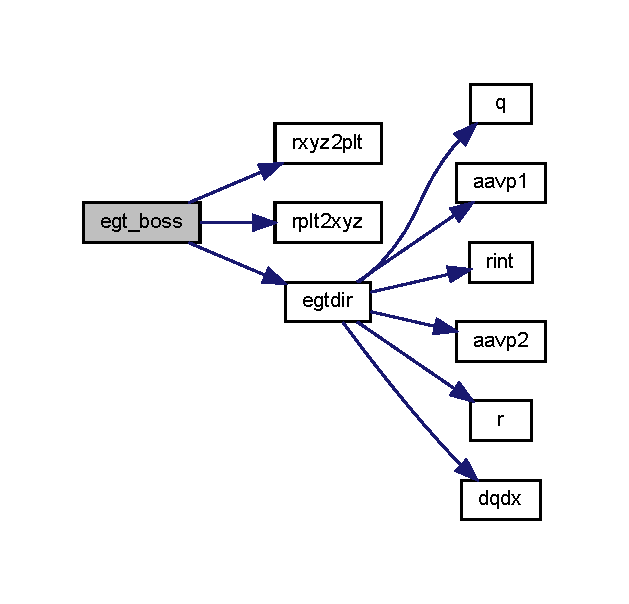
\includegraphics[width=302pt]{Leroi_8f90_a1b3954d66e2114dd2d6b6a5a44b7f0a4_cgraph}
\end{center}
\end{figure}
Here is the caller graph for this function\+:\nopagebreak
\begin{figure}[H]
\begin{center}
\leavevmode
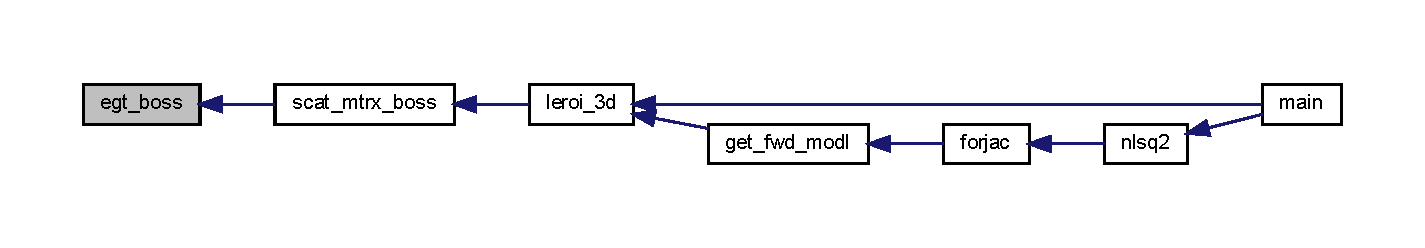
\includegraphics[width=350pt]{Leroi_8f90_a1b3954d66e2114dd2d6b6a5a44b7f0a4_icgraph}
\end{center}
\end{figure}
\mbox{\Hypertarget{Leroi_8f90_a39b25039701be699f724d2a872d3d3f3}\label{Leroi_8f90_a39b25039701be699f724d2a872d3d3f3}} 
\index{Leroi.\+f90@{Leroi.\+f90}!egt\+\_\+cspl@{egt\+\_\+cspl}}
\index{egt\+\_\+cspl@{egt\+\_\+cspl}!Leroi.\+f90@{Leroi.\+f90}}
\subsubsection{\texorpdfstring{egt\+\_\+cspl()}{egt\_cspl()}}
{\footnotesize\ttfamily subroutine egt\+\_\+cspl (\begin{DoxyParamCaption}\item[{integer}]{N\+R\+E\+GT,  }\item[{real, dimension(nregt)}]{R\+H\+O\+T\+RP,  }\item[{integer}]{N\+L\+YR,  }\item[{real (kind=ql), dimension(nlyr)}]{T\+H\+KD,  }\item[{real (kind=ql), dimension(0\+:nlyr)}]{R\+M\+UD,  }\item[{complex(kind=ql), dimension(nlyr)}]{S\+I\+GL,  }\item[{complex(kind=ql), dimension(nlyr)}]{K\+S\+QL,  }\item[{real}]{Z\+TR,  }\item[{real, dimension (4,nregt)}]{G\+R1,  }\item[{real, dimension (4,nregt)}]{G\+I1,  }\item[{real, dimension (4,nregt)}]{G\+R2,  }\item[{real, dimension (4,nregt)}]{G\+I2,  }\item[{real, dimension (4,nregt)}]{G\+R3,  }\item[{real, dimension (4,nregt)}]{G\+I3,  }\item[{real, dimension (4,nregt)}]{G\+R4,  }\item[{real, dimension (4,nregt)}]{G\+I4,  }\item[{real, dimension (4,nregt)}]{G\+R5,  }\item[{real, dimension (4,nregt)}]{G\+I5,  }\item[{real, dimension (4,nregt)}]{G\+R6,  }\item[{real, dimension (4,nregt)}]{G\+I6 }\end{DoxyParamCaption})}

Here is the call graph for this function\+:\nopagebreak
\begin{figure}[H]
\begin{center}
\leavevmode
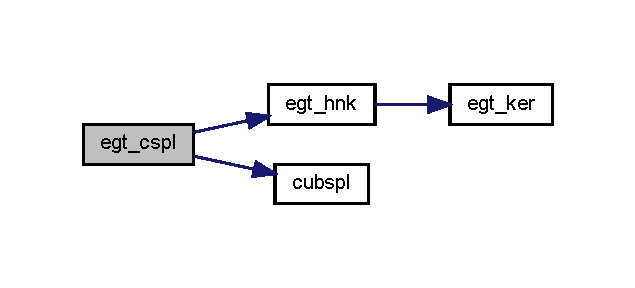
\includegraphics[width=305pt]{Leroi_8f90_a39b25039701be699f724d2a872d3d3f3_cgraph}
\end{center}
\end{figure}
Here is the caller graph for this function\+:\nopagebreak
\begin{figure}[H]
\begin{center}
\leavevmode
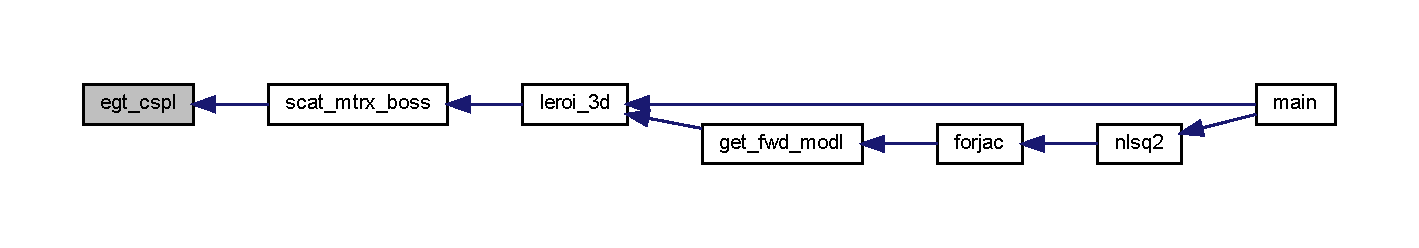
\includegraphics[width=350pt]{Leroi_8f90_a39b25039701be699f724d2a872d3d3f3_icgraph}
\end{center}
\end{figure}
\mbox{\Hypertarget{Leroi_8f90_ae50e88569c7037d3d431d0b0dd30c795}\label{Leroi_8f90_ae50e88569c7037d3d431d0b0dd30c795}} 
\index{Leroi.\+f90@{Leroi.\+f90}!egt\+\_\+hnk@{egt\+\_\+hnk}}
\index{egt\+\_\+hnk@{egt\+\_\+hnk}!Leroi.\+f90@{Leroi.\+f90}}
\subsubsection{\texorpdfstring{egt\+\_\+hnk()}{egt\_hnk()}}
{\footnotesize\ttfamily subroutine egt\+\_\+hnk (\begin{DoxyParamCaption}\item[{integer}]{N\+R\+HO,  }\item[{real, dimension(nrho)}]{R\+H\+O\+T\+RP,  }\item[{integer}]{N\+L\+YR,  }\item[{real(kind=ql), dimension(nlyr)}]{T\+H\+KD,  }\item[{real(kind=ql), dimension(0\+:nlyr)}]{R\+M\+UD,  }\item[{complex(kind=ql), dimension(nlyr)}]{S\+I\+GL,  }\item[{complex(kind=ql), dimension(nlyr)}]{K\+S\+QL,  }\item[{real}]{Z\+TR,  }\item[{complex(kind=ql), dimension(nrho,6)}]{E\+H\+RI }\end{DoxyParamCaption})}

Here is the call graph for this function\+:\nopagebreak
\begin{figure}[H]
\begin{center}
\leavevmode
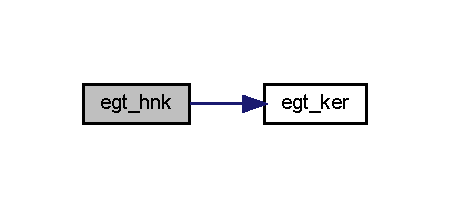
\includegraphics[width=216pt]{Leroi_8f90_ae50e88569c7037d3d431d0b0dd30c795_cgraph}
\end{center}
\end{figure}
Here is the caller graph for this function\+:\nopagebreak
\begin{figure}[H]
\begin{center}
\leavevmode
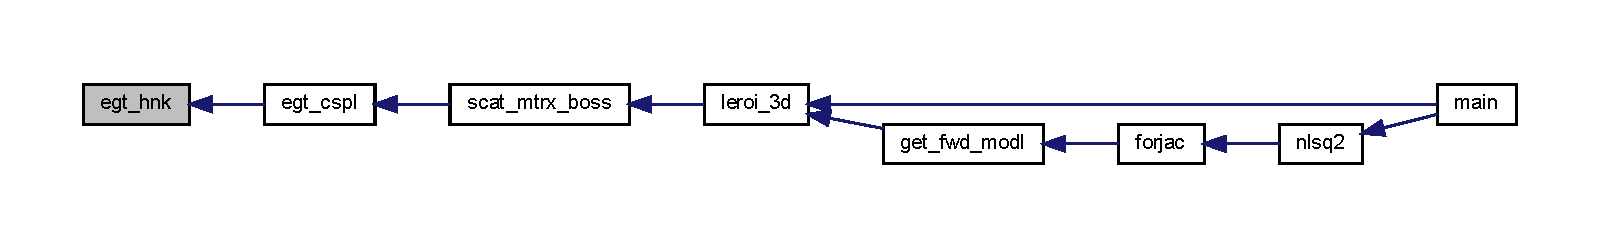
\includegraphics[width=350pt]{Leroi_8f90_ae50e88569c7037d3d431d0b0dd30c795_icgraph}
\end{center}
\end{figure}
\mbox{\Hypertarget{Leroi_8f90_ad8346887f578fa81508d64ff7308bd70}\label{Leroi_8f90_ad8346887f578fa81508d64ff7308bd70}} 
\index{Leroi.\+f90@{Leroi.\+f90}!egt\+\_\+ker@{egt\+\_\+ker}}
\index{egt\+\_\+ker@{egt\+\_\+ker}!Leroi.\+f90@{Leroi.\+f90}}
\subsubsection{\texorpdfstring{egt\+\_\+ker()}{egt\_ker()}}
{\footnotesize\ttfamily subroutine egt\+\_\+ker (\begin{DoxyParamCaption}\item[{integer}]{N\+R\+HO,  }\item[{integer}]{K,  }\item[{integer}]{JR,  }\item[{integer}]{L,  }\item[{real (kind=ql)}]{L\+M\+B\+DA,  }\item[{integer}]{N\+L\+YR,  }\item[{real (kind=ql), dimension(nlyr)}]{T\+H\+KD,  }\item[{real (kind=ql), dimension(0\+:nlyr)}]{R\+M\+UD,  }\item[{complex (kind=ql), dimension(nlyr)}]{S\+I\+GL,  }\item[{complex (kind=ql), dimension(nlyr)}]{K\+S\+QL,  }\item[{real (kind=ql)}]{Z\+T\+RD,  }\item[{complex (kind=ql), dimension(jnlo-\/nrho\+:jnhi,6)}]{K\+ER,  }\item[{complex (kind=ql), dimension(nrho,6)}]{E\+H\+RI,  }\item[{logical}]{J\+U\+MP }\end{DoxyParamCaption})}

Here is the caller graph for this function\+:\nopagebreak
\begin{figure}[H]
\begin{center}
\leavevmode
\includegraphics[width=350pt]{Leroi_8f90_ad8346887f578fa81508d64ff7308bd70_icgraph}
\end{center}
\end{figure}
\mbox{\Hypertarget{Leroi_8f90_a7acbe12b71ec5be34d994fc6743480c8}\label{Leroi_8f90_a7acbe12b71ec5be34d994fc6743480c8}} 
\index{Leroi.\+f90@{Leroi.\+f90}!egt\+\_\+pl\+\_\+boss@{egt\+\_\+pl\+\_\+boss}}
\index{egt\+\_\+pl\+\_\+boss@{egt\+\_\+pl\+\_\+boss}!Leroi.\+f90@{Leroi.\+f90}}
\subsubsection{\texorpdfstring{egt\+\_\+pl\+\_\+boss()}{egt\_pl\_boss()}}
{\footnotesize\ttfamily subroutine egt\+\_\+pl\+\_\+boss (\begin{DoxyParamCaption}\item[{integer}]{N\+AL,  }\item[{integer}]{N\+BL,  }\item[{integer}]{N\+AB,  }\item[{real}]{D\+AL,  }\item[{real}]{D\+BL,  }\item[{complex}]{K\+S\+QN,  }\item[{real}]{D\+P\+T\+HB,  }\item[{real}]{P\+T\+O\+PL,  }\item[{real}]{C\+DP,  }\item[{real}]{S\+DP,  }\item[{real}]{C\+PL,  }\item[{real}]{S\+PL,  }\item[{integer}]{N\+Z2,  }\item[{real, dimension(nz2)}]{Z\+V2,  }\item[{integer}]{N\+R\+E\+GT,  }\item[{real, dimension(nregt)}]{R\+H\+O\+T\+RP,  }\item[{real, dimension(4,nregt,nz2)}]{G\+R1Z,  }\item[{real, dimension(4,nregt,nz2)}]{G\+I1Z,  }\item[{real, dimension(4,nregt,nz2)}]{G\+R2Z,  }\item[{real, dimension(4,nregt,nz2)}]{G\+I2Z,  }\item[{real, dimension(4,nregt,nz2)}]{G\+R3Z,  }\item[{real, dimension(4,nregt,nz2)}]{G\+I3Z,  }\item[{real, dimension(4,nregt,nz2)}]{G\+R4Z,  }\item[{real, dimension(4,nregt,nz2)}]{G\+I4Z,  }\item[{real, dimension(4,nregt,nz2)}]{G\+R5Z,  }\item[{real, dimension(4,nregt,nz2)}]{G\+I5Z,  }\item[{real, dimension(4,nregt,nz2)}]{G\+R6Z,  }\item[{real, dimension(4,nregt,nz2)}]{G\+I6Z,  }\item[{complex, dimension(nbl,nbl,nal,nal)}]{S\+AA,  }\item[{complex, dimension(nbl,nbl,nal,nal)}]{S\+BA,  }\item[{complex, dimension(nbl,nbl,nal,nal)}]{S\+BB,  }\item[{complex, dimension(nbl,nbl,nal,nal)}]{V\+AA,  }\item[{complex, dimension(nbl,nbl,nal,nal)}]{V\+AB,  }\item[{complex, dimension(nbl,nbl,nal,nal)}]{V\+BA,  }\item[{complex, dimension(nbl,nbl,nal,nal)}]{V\+BB }\end{DoxyParamCaption})}

Here is the call graph for this function\+:\nopagebreak
\begin{figure}[H]
\begin{center}
\leavevmode
\includegraphics[width=315pt]{Leroi_8f90_a7acbe12b71ec5be34d994fc6743480c8_cgraph}
\end{center}
\end{figure}
Here is the caller graph for this function\+:\nopagebreak
\begin{figure}[H]
\begin{center}
\leavevmode
\includegraphics[width=350pt]{Leroi_8f90_a7acbe12b71ec5be34d994fc6743480c8_icgraph}
\end{center}
\end{figure}
\mbox{\Hypertarget{Leroi_8f90_a9074cfabdfb82294ca3b8541c14a9099}\label{Leroi_8f90_a9074cfabdfb82294ca3b8541c14a9099}} 
\index{Leroi.\+f90@{Leroi.\+f90}!egt\+\_\+ul\+\_\+boss@{egt\+\_\+ul\+\_\+boss}}
\index{egt\+\_\+ul\+\_\+boss@{egt\+\_\+ul\+\_\+boss}!Leroi.\+f90@{Leroi.\+f90}}
\subsubsection{\texorpdfstring{egt\+\_\+ul\+\_\+boss()}{egt\_ul\_boss()}}
{\footnotesize\ttfamily subroutine egt\+\_\+ul\+\_\+boss (\begin{DoxyParamCaption}\item[{integer}]{N\+L\+YR,  }\item[{real (kind=ql), dimension(nlyr)}]{T\+H\+KD,  }\item[{real (kind=ql), dimension(nlyr)}]{D\+P\+T\+HL,  }\item[{real (kind=ql), dimension(0\+:nlyr)}]{R\+M\+UD,  }\item[{complex(kind=ql), dimension(nlyr)}]{S\+I\+GL,  }\item[{complex(kind=ql), dimension(nlyr)}]{K\+S\+QL,  }\item[{integer}]{N\+AL,  }\item[{integer}]{N\+BL,  }\item[{integer}]{N\+AB,  }\item[{real}]{D\+AL,  }\item[{real}]{D\+BL,  }\item[{real, dimension(nab)}]{X\+C\+E\+L1,  }\item[{real, dimension(nab)}]{Y\+C\+E\+L1,  }\item[{real, dimension(nbl)}]{Z\+C1L,  }\item[{integer}]{R\+X\+L\+YR,  }\item[{real}]{C\+DP,  }\item[{real}]{S\+DP,  }\item[{integer}]{N\+R\+E\+GT,  }\item[{real, dimension(nregt)}]{R\+H\+O\+T\+RP,  }\item[{complex, dimension(nbl,nbl,nal,nal)}]{S\+AA,  }\item[{complex, dimension(nbl,nbl,nal,nal)}]{S\+BA,  }\item[{complex, dimension(nbl,nbl,nal,nal)}]{S\+BB,  }\item[{complex, dimension(nbl,nbl,nal,nal)}]{V\+AA,  }\item[{complex, dimension(nbl,nbl,nal,nal)}]{V\+AB,  }\item[{complex, dimension(nbl,nbl,nal,nal)}]{V\+BA,  }\item[{complex, dimension(nbl,nbl,nal,nal)}]{V\+BB }\end{DoxyParamCaption})}

Here is the call graph for this function\+:\nopagebreak
\begin{figure}[H]
\begin{center}
\leavevmode
\includegraphics[width=350pt]{Leroi_8f90_a9074cfabdfb82294ca3b8541c14a9099_cgraph}
\end{center}
\end{figure}
Here is the caller graph for this function\+:\nopagebreak
\begin{figure}[H]
\begin{center}
\leavevmode
\includegraphics[width=350pt]{Leroi_8f90_a9074cfabdfb82294ca3b8541c14a9099_icgraph}
\end{center}
\end{figure}
\mbox{\Hypertarget{Leroi_8f90_a55b57146ea180fed3080a010421620fe}\label{Leroi_8f90_a55b57146ea180fed3080a010421620fe}} 
\index{Leroi.\+f90@{Leroi.\+f90}!egt\+\_\+ul\+\_\+cspl@{egt\+\_\+ul\+\_\+cspl}}
\index{egt\+\_\+ul\+\_\+cspl@{egt\+\_\+ul\+\_\+cspl}!Leroi.\+f90@{Leroi.\+f90}}
\subsubsection{\texorpdfstring{egt\+\_\+ul\+\_\+cspl()}{egt\_ul\_cspl()}}
{\footnotesize\ttfamily subroutine egt\+\_\+ul\+\_\+cspl (\begin{DoxyParamCaption}\item[{integer}]{N\+R\+E\+GT,  }\item[{real, dimension(nregt)}]{R\+H\+O\+T\+RP,  }\item[{integer}]{S\+X\+L\+YR,  }\item[{integer}]{R\+X\+L\+YR,  }\item[{integer}]{K\+FG,  }\item[{integer}]{N\+L\+YR,  }\item[{real(kind=ql), dimension (nlyr)}]{T\+H\+KD,  }\item[{real(kind=ql), dimension (nlyr)}]{D\+P\+T\+HL,  }\item[{real (kind=ql), dimension(0\+:nlyr)}]{R\+M\+UD,  }\item[{complex(kind=ql), dimension(nlyr)}]{S\+I\+GL,  }\item[{complex(kind=ql), dimension(nlyr)}]{K\+S\+QL,  }\item[{real (kind=ql)}]{ZS,  }\item[{real (kind=ql)}]{ZR,  }\item[{real, dimension (4,nregt)}]{Q\+R1,  }\item[{real, dimension (4,nregt)}]{Q\+I1,  }\item[{real, dimension (4,nregt)}]{Q\+R2,  }\item[{real, dimension (4,nregt)}]{Q\+I2,  }\item[{real, dimension (4,nregt)}]{Q\+R3,  }\item[{real, dimension (4,nregt)}]{Q\+I3,  }\item[{real, dimension (4,nregt)}]{Q\+R4,  }\item[{real, dimension (4,nregt)}]{Q\+I4,  }\item[{real, dimension (4,nregt)}]{Q\+R5,  }\item[{real, dimension (4,nregt)}]{Q\+I5,  }\item[{real, dimension (4,nregt)}]{Q\+R6,  }\item[{real, dimension (4,nregt)}]{Q\+I6,  }\item[{real, dimension (4,nregt)}]{Q\+R7,  }\item[{real, dimension (4,nregt)}]{Q\+I7 }\end{DoxyParamCaption})}

Here is the call graph for this function\+:\nopagebreak
\begin{figure}[H]
\begin{center}
\leavevmode
\includegraphics[width=350pt]{Leroi_8f90_a55b57146ea180fed3080a010421620fe_cgraph}
\end{center}
\end{figure}
Here is the caller graph for this function\+:\nopagebreak
\begin{figure}[H]
\begin{center}
\leavevmode
\includegraphics[width=350pt]{Leroi_8f90_a55b57146ea180fed3080a010421620fe_icgraph}
\end{center}
\end{figure}
\mbox{\Hypertarget{Leroi_8f90_a1d1da4021109f56adcc9ad84d89cd1b7}\label{Leroi_8f90_a1d1da4021109f56adcc9ad84d89cd1b7}} 
\index{Leroi.\+f90@{Leroi.\+f90}!egt\+\_\+ul\+\_\+hnk@{egt\+\_\+ul\+\_\+hnk}}
\index{egt\+\_\+ul\+\_\+hnk@{egt\+\_\+ul\+\_\+hnk}!Leroi.\+f90@{Leroi.\+f90}}
\subsubsection{\texorpdfstring{egt\+\_\+ul\+\_\+hnk()}{egt\_ul\_hnk()}}
{\footnotesize\ttfamily subroutine egt\+\_\+ul\+\_\+hnk (\begin{DoxyParamCaption}\item[{integer}]{N\+R\+E\+GT,  }\item[{real, dimension(nregt)}]{R\+H\+O\+T\+RP,  }\item[{integer}]{S\+X\+L\+YR,  }\item[{integer}]{R\+X\+L\+YR,  }\item[{integer}]{K\+FG,  }\item[{integer}]{N\+L\+YR,  }\item[{real(kind=ql), dimension (nlyr)}]{T\+H\+KD,  }\item[{real(kind=ql), dimension (nlyr)}]{D\+P\+T\+HL,  }\item[{real(kind=ql), dimension(0\+:nlyr)}]{R\+M\+UD,  }\item[{complex(kind=ql), dimension (nlyr)}]{S\+I\+GL,  }\item[{complex(kind=ql), dimension (nlyr)}]{K\+S\+QL,  }\item[{real(kind=ql)}]{ZS,  }\item[{real(kind=ql)}]{ZR,  }\item[{complex(kind=ql), dimension(nregt,7)}]{G\+T\+ED }\end{DoxyParamCaption})}

Here is the call graph for this function\+:\nopagebreak
\begin{figure}[H]
\begin{center}
\leavevmode
\includegraphics[width=350pt]{Leroi_8f90_a1d1da4021109f56adcc9ad84d89cd1b7_cgraph}
\end{center}
\end{figure}
Here is the caller graph for this function\+:\nopagebreak
\begin{figure}[H]
\begin{center}
\leavevmode
\includegraphics[width=350pt]{Leroi_8f90_a1d1da4021109f56adcc9ad84d89cd1b7_icgraph}
\end{center}
\end{figure}
\mbox{\Hypertarget{Leroi_8f90_a8f7098d7bc36902fbbda312874c15120}\label{Leroi_8f90_a8f7098d7bc36902fbbda312874c15120}} 
\index{Leroi.\+f90@{Leroi.\+f90}!egt\+\_\+ul\+\_\+ker@{egt\+\_\+ul\+\_\+ker}}
\index{egt\+\_\+ul\+\_\+ker@{egt\+\_\+ul\+\_\+ker}!Leroi.\+f90@{Leroi.\+f90}}
\subsubsection{\texorpdfstring{egt\+\_\+ul\+\_\+ker()}{egt\_ul\_ker()}}
{\footnotesize\ttfamily subroutine egt\+\_\+ul\+\_\+ker (\begin{DoxyParamCaption}\item[{integer}]{N\+R\+E\+GT,  }\item[{integer}]{K,  }\item[{integer}]{JR,  }\item[{integer}]{L,  }\item[{real(kind=ql)}]{L\+M\+B\+DA,  }\item[{integer}]{S\+X\+L\+YR,  }\item[{integer}]{R\+X\+L\+YR,  }\item[{integer}]{K\+FG,  }\item[{integer}]{N\+L\+YR,  }\item[{real(kind=ql), dimension (nlyr)}]{T\+H\+KD,  }\item[{real(kind=ql), dimension (nlyr)}]{D\+P\+T\+HL,  }\item[{real(kind=ql), dimension(0\+:nlyr)}]{R\+M\+UD,  }\item[{complex(kind=ql), dimension (nlyr)}]{S\+I\+GL,  }\item[{complex(kind=ql), dimension (nlyr)}]{K\+S\+QL,  }\item[{real(kind=ql)}]{ZS,  }\item[{real(kind=ql)}]{ZR,  }\item[{complex (kind=ql), dimension(jnlo-\/nregt\+:jnhi,7)}]{K\+ER,  }\item[{complex (kind=ql), dimension(nregt,7)}]{G\+T\+ED,  }\item[{logical}]{J\+U\+MP }\end{DoxyParamCaption})}

Here is the call graph for this function\+:\nopagebreak
\begin{figure}[H]
\begin{center}
\leavevmode
\includegraphics[width=335pt]{Leroi_8f90_a8f7098d7bc36902fbbda312874c15120_cgraph}
\end{center}
\end{figure}
Here is the caller graph for this function\+:\nopagebreak
\begin{figure}[H]
\begin{center}
\leavevmode
\includegraphics[width=350pt]{Leroi_8f90_a8f7098d7bc36902fbbda312874c15120_icgraph}
\end{center}
\end{figure}
\mbox{\Hypertarget{Leroi_8f90_a24151574c4bb3d7844db88f91d23b589}\label{Leroi_8f90_a24151574c4bb3d7844db88f91d23b589}} 
\index{Leroi.\+f90@{Leroi.\+f90}!egtdir@{egtdir}}
\index{egtdir@{egtdir}!Leroi.\+f90@{Leroi.\+f90}}
\subsubsection{\texorpdfstring{egtdir()}{egtdir()}}
{\footnotesize\ttfamily subroutine egtdir (\begin{DoxyParamCaption}\item[{integer, intent(in)}]{JB,  }\item[{integer, intent(in)}]{JA,  }\item[{complex, intent(in)}]{K\+B\+A\+SE,  }\item[{real, intent(in)}]{D\+AL,  }\item[{real, intent(in)}]{D\+BL,  }\item[{complex, intent(out)}]{A\+AS,  }\item[{complex, intent(out)}]{A\+AV,  }\item[{complex, intent(out)}]{A\+BV,  }\item[{complex, intent(out)}]{B\+BV }\end{DoxyParamCaption})}

Here is the call graph for this function\+:\nopagebreak
\begin{figure}[H]
\begin{center}
\leavevmode
\includegraphics[width=200pt]{Leroi_8f90_a24151574c4bb3d7844db88f91d23b589_cgraph}
\end{center}
\end{figure}
Here is the caller graph for this function\+:\nopagebreak
\begin{figure}[H]
\begin{center}
\leavevmode
\includegraphics[width=350pt]{Leroi_8f90_a24151574c4bb3d7844db88f91d23b589_icgraph}
\end{center}
\end{figure}
\mbox{\Hypertarget{Leroi_8f90_a7312ba6fbf8b492624e2663b1255893f}\label{Leroi_8f90_a7312ba6fbf8b492624e2663b1255893f}} 
\index{Leroi.\+f90@{Leroi.\+f90}!egtrx\+\_\+boss@{egtrx\+\_\+boss}}
\index{egtrx\+\_\+boss@{egtrx\+\_\+boss}!Leroi.\+f90@{Leroi.\+f90}}
\subsubsection{\texorpdfstring{egtrx\+\_\+boss()}{egtrx\_boss()}}
{\footnotesize\ttfamily subroutine egtrx\+\_\+boss (\begin{DoxyParamCaption}\item[{integer}]{N\+P\+LT,  }\item[{integer, dimension (nplt)}]{P\+L\+YR,  }\item[{integer}]{M\+X\+AB,  }\item[{integer, dimension (nplt)}]{NA,  }\item[{integer, dimension (nplt)}]{NB,  }\item[{real, dimension (nplt)}]{P\+L\+A\+ZM,  }\item[{real, dimension (nplt)}]{P\+L\+D\+IP,  }\item[{real, dimension (nplt)}]{P\+L\+U\+NJ,  }\item[{real, dimension (mxab,nplt)}]{X\+C\+E\+LL,  }\item[{real, dimension (mxab,nplt)}]{Y\+C\+E\+LL,  }\item[{real, dimension (mxab,nplt)}]{Z\+C\+E\+LL,  }\item[{integer}]{N\+L\+YR,  }\item[{real (kind=ql), dimension(nlyr)}]{T\+H\+KD,  }\item[{real (kind=ql), dimension(nlyr)}]{D\+P\+T\+HL,  }\item[{real (kind=ql), dimension(0\+:nlyr)}]{R\+M\+UD,  }\item[{complex(kind=ql), dimension(nlyr)}]{S\+I\+GL,  }\item[{complex(kind=ql), dimension(nlyr)}]{K\+S\+QL,  }\item[{integer}]{N\+TX,  }\item[{integer}]{M\+R\+X\+TX,  }\item[{integer, dimension(ntx)}]{N\+R\+X\+TX,  }\item[{integer, dimension(mrxtx,ntx)}]{R\+X\+ID,  }\item[{integer}]{M\+X\+RS,  }\item[{integer, dimension(mrxtx,ntx)}]{N\+RS,  }\item[{real, dimension (mxrs,mrxtx,ntx)}]{X\+RS,  }\item[{real, dimension (mxrs,mrxtx,ntx)}]{Y\+RS,  }\item[{real, dimension (mrxtx,ntx)}]{Z\+R\+X\+TX,  }\item[{real, dimension (mxrs,mrxtx,ntx)}]{W\+T\+RS,  }\item[{integer}]{N\+R\+M\+GT,  }\item[{real, dimension(nrmgt)}]{R\+H\+O\+T\+RP,  }\item[{integer}]{N\+Z1,  }\item[{real, dimension(nz1)}]{Z\+V1,  }\item[{integer}]{N\+M\+GP,  }\item[{real, dimension (nmgp,nplt)}]{X\+MG,  }\item[{real, dimension (nmgp,nplt)}]{Y\+MG,  }\item[{real, dimension (nmgp,nplt)}]{Z\+MG,  }\item[{real, dimension (nplt)}]{W\+MG,  }\item[{complex, dimension (mxab,3,mrxtx,ntx,nplt)}]{HA,  }\item[{complex, dimension (mxab,3,mrxtx,ntx,nplt)}]{HB }\end{DoxyParamCaption})}

Here is the call graph for this function\+:\nopagebreak
\begin{figure}[H]
\begin{center}
\leavevmode
\includegraphics[width=350pt]{Leroi_8f90_a7312ba6fbf8b492624e2663b1255893f_cgraph}
\end{center}
\end{figure}
Here is the caller graph for this function\+:\nopagebreak
\begin{figure}[H]
\begin{center}
\leavevmode
\includegraphics[width=350pt]{Leroi_8f90_a7312ba6fbf8b492624e2663b1255893f_icgraph}
\end{center}
\end{figure}
\mbox{\Hypertarget{Leroi_8f90_a1770320680e91059231180f0654cce66}\label{Leroi_8f90_a1770320680e91059231180f0654cce66}} 
\index{Leroi.\+f90@{Leroi.\+f90}!egtrx\+\_\+boss\+\_\+ul@{egtrx\+\_\+boss\+\_\+ul}}
\index{egtrx\+\_\+boss\+\_\+ul@{egtrx\+\_\+boss\+\_\+ul}!Leroi.\+f90@{Leroi.\+f90}}
\subsubsection{\texorpdfstring{egtrx\+\_\+boss\+\_\+ul()}{egtrx\_boss\_ul()}}
{\footnotesize\ttfamily subroutine egtrx\+\_\+boss\+\_\+ul (\begin{DoxyParamCaption}\item[{integer}]{JP,  }\item[{integer}]{S\+X\+L\+YR,  }\item[{integer}]{N\+P\+LT,  }\item[{integer}]{M\+X\+AB,  }\item[{integer}]{N\+AL,  }\item[{integer}]{N\+BL,  }\item[{real}]{D\+AL,  }\item[{real}]{D\+BL,  }\item[{real, dimension (nplt)}]{P\+L\+A\+ZM,  }\item[{real, dimension (nplt)}]{P\+L\+D\+IP,  }\item[{real, dimension (mxab,nplt)}]{X\+C\+E\+LL,  }\item[{real, dimension (mxab,nplt)}]{Y\+C\+E\+LL,  }\item[{integer}]{N\+L\+YR,  }\item[{real (kind=ql), dimension(nlyr)}]{T\+H\+KD,  }\item[{real (kind=ql), dimension(nlyr)}]{D\+P\+T\+HL,  }\item[{real (kind=ql), dimension(0\+:nlyr)}]{R\+M\+UD,  }\item[{complex(kind=ql), dimension(nlyr)}]{S\+I\+GL,  }\item[{complex(kind=ql), dimension(nlyr)}]{K\+S\+QL,  }\item[{integer}]{N\+TX,  }\item[{integer}]{M\+R\+X\+TX,  }\item[{integer, dimension(ntx)}]{N\+R\+X\+TX,  }\item[{integer, dimension(mrxtx,ntx)}]{R\+X\+ID,  }\item[{integer}]{M\+X\+RS,  }\item[{integer, dimension(mrxtx,ntx)}]{N\+RS,  }\item[{real, dimension (mxrs,mrxtx,ntx)}]{X\+RS,  }\item[{real, dimension (mxrs,mrxtx,ntx)}]{Y\+RS,  }\item[{real, dimension (mrxtx,ntx)}]{Z\+R\+X\+TX,  }\item[{real, dimension (mxrs,mrxtx,ntx)}]{W\+T\+RS,  }\item[{integer}]{N\+R\+M\+GT,  }\item[{real, dimension(nrmgt)}]{R\+H\+O\+T\+RP,  }\item[{integer}]{N\+Z3L,  }\item[{real, dimension(nz3l)}]{Z\+C3L,  }\item[{complex, dimension (mxab,3,mrxtx,ntx,nplt)}]{HA,  }\item[{complex, dimension (mxab,3,mrxtx,ntx,nplt)}]{HB }\end{DoxyParamCaption})}

Here is the call graph for this function\+:\nopagebreak
\begin{figure}[H]
\begin{center}
\leavevmode
\includegraphics[width=350pt]{Leroi_8f90_a1770320680e91059231180f0654cce66_cgraph}
\end{center}
\end{figure}
Here is the caller graph for this function\+:\nopagebreak
\begin{figure}[H]
\begin{center}
\leavevmode
\includegraphics[width=350pt]{Leroi_8f90_a1770320680e91059231180f0654cce66_icgraph}
\end{center}
\end{figure}
\mbox{\Hypertarget{Leroi_8f90_a10fd9ada0ec15151a8112666c09a245d}\label{Leroi_8f90_a10fd9ada0ec15151a8112666c09a245d}} 
\index{Leroi.\+f90@{Leroi.\+f90}!egtrx\+\_\+cspl@{egtrx\+\_\+cspl}}
\index{egtrx\+\_\+cspl@{egtrx\+\_\+cspl}!Leroi.\+f90@{Leroi.\+f90}}
\subsubsection{\texorpdfstring{egtrx\+\_\+cspl()}{egtrx\_cspl()}}
{\footnotesize\ttfamily subroutine egtrx\+\_\+cspl (\begin{DoxyParamCaption}\item[{integer}]{N\+R\+M\+GT,  }\item[{real, dimension(nrmgt)}]{R\+H\+O\+T\+RP,  }\item[{integer}]{S\+X\+L\+YR,  }\item[{integer}]{R\+X\+L\+YR,  }\item[{integer}]{K\+FG,  }\item[{integer}]{N\+L\+YR,  }\item[{real (kind=ql), dimension(nlyr)}]{T\+H\+KD,  }\item[{real (kind=ql), dimension(nlyr)}]{D\+P\+T\+HL,  }\item[{real (kind=ql), dimension(0\+:nlyr)}]{R\+M\+UD,  }\item[{complex(kind=ql), dimension(nlyr)}]{S\+I\+GL,  }\item[{complex(kind=ql), dimension(nlyr)}]{K\+S\+QL,  }\item[{real (kind=ql)}]{ZR,  }\item[{integer}]{NZ,  }\item[{real, dimension(nz)}]{ZV,  }\item[{integer}]{N\+I\+N\+TG,  }\item[{real, dimension (4,nrmgt,nz)}]{Q\+B1R,  }\item[{real, dimension (4,nrmgt,nz)}]{Q\+B1I,  }\item[{real, dimension (4,nrmgt,nz)}]{Q\+B2R,  }\item[{real, dimension (4,nrmgt,nz)}]{Q\+B2I,  }\item[{real, dimension (4,nrmgt,nz)}]{Q\+B3R,  }\item[{real, dimension (4,nrmgt,nz)}]{Q\+B3I,  }\item[{real, dimension (4,nrmgt,nz)}]{Q\+B4R,  }\item[{real, dimension (4,nrmgt,nz)}]{Q\+B4I,  }\item[{real, dimension (4,nrmgt,nz)}]{Q\+B5R,  }\item[{real, dimension (4,nrmgt,nz)}]{Q\+B5I,  }\item[{real, dimension (4,nrmgt,nz)}]{Q\+B6R,  }\item[{real, dimension (4,nrmgt,nz)}]{Q\+B6I }\end{DoxyParamCaption})}

Here is the call graph for this function\+:\nopagebreak
\begin{figure}[H]
\begin{center}
\leavevmode
\includegraphics[width=350pt]{Leroi_8f90_a10fd9ada0ec15151a8112666c09a245d_cgraph}
\end{center}
\end{figure}
Here is the caller graph for this function\+:\nopagebreak
\begin{figure}[H]
\begin{center}
\leavevmode
\includegraphics[width=350pt]{Leroi_8f90_a10fd9ada0ec15151a8112666c09a245d_icgraph}
\end{center}
\end{figure}
\mbox{\Hypertarget{Leroi_8f90_a6bbebe0c58cc288fcd56628de8860916}\label{Leroi_8f90_a6bbebe0c58cc288fcd56628de8860916}} 
\index{Leroi.\+f90@{Leroi.\+f90}!egtrx\+\_\+dir@{egtrx\+\_\+dir}}
\index{egtrx\+\_\+dir@{egtrx\+\_\+dir}!Leroi.\+f90@{Leroi.\+f90}}
\subsubsection{\texorpdfstring{egtrx\+\_\+dir()}{egtrx\_dir()}}
{\footnotesize\ttfamily subroutine egtrx\+\_\+dir (\begin{DoxyParamCaption}\item[{real}]{XD,  }\item[{real}]{YD,  }\item[{real}]{ZD,  }\item[{complex}]{KB,  }\item[{complex}]{E\+XX,  }\item[{complex}]{E\+XY,  }\item[{complex}]{E\+XZ,  }\item[{complex}]{E\+YY,  }\item[{complex}]{E\+YZ,  }\item[{complex}]{E\+ZZ }\end{DoxyParamCaption})}

Here is the caller graph for this function\+:\nopagebreak
\begin{figure}[H]
\begin{center}
\leavevmode
\includegraphics[width=350pt]{Leroi_8f90_a6bbebe0c58cc288fcd56628de8860916_icgraph}
\end{center}
\end{figure}
\mbox{\Hypertarget{Leroi_8f90_a5489646b1d19d3a2a814c56265bd78fb}\label{Leroi_8f90_a5489646b1d19d3a2a814c56265bd78fb}} 
\index{Leroi.\+f90@{Leroi.\+f90}!egtrx\+\_\+hnk@{egtrx\+\_\+hnk}}
\index{egtrx\+\_\+hnk@{egtrx\+\_\+hnk}!Leroi.\+f90@{Leroi.\+f90}}
\subsubsection{\texorpdfstring{egtrx\+\_\+hnk()}{egtrx\_hnk()}}
{\footnotesize\ttfamily subroutine egtrx\+\_\+hnk (\begin{DoxyParamCaption}\item[{integer}]{N\+R\+M\+GT,  }\item[{real, dimension(nrmgt)}]{R\+H\+O\+T\+RP,  }\item[{integer}]{S\+X\+L\+YR,  }\item[{integer}]{R\+X\+L\+YR,  }\item[{integer}]{K\+FG,  }\item[{integer}]{N\+L\+YR,  }\item[{real (kind=ql), dimension(nlyr)}]{T\+H\+KD,  }\item[{real (kind=ql), dimension(nlyr)}]{D\+P\+T\+HL,  }\item[{complex(kind=ql), dimension(nlyr)}]{S\+I\+GL,  }\item[{complex(kind=ql), dimension(nlyr)}]{K\+S\+QL,  }\item[{real (kind=ql), dimension(0\+:nlyr)}]{R\+M\+UD,  }\item[{real (kind=ql)}]{ZR,  }\item[{real (kind=ql)}]{ZS,  }\item[{integer}]{N\+I\+N\+TG,  }\item[{complex (kind=ql), dimension(nrmgt,6)}]{E\+H\+RI }\end{DoxyParamCaption})}

Here is the call graph for this function\+:\nopagebreak
\begin{figure}[H]
\begin{center}
\leavevmode
\includegraphics[width=350pt]{Leroi_8f90_a5489646b1d19d3a2a814c56265bd78fb_cgraph}
\end{center}
\end{figure}
Here is the caller graph for this function\+:\nopagebreak
\begin{figure}[H]
\begin{center}
\leavevmode
\includegraphics[width=350pt]{Leroi_8f90_a5489646b1d19d3a2a814c56265bd78fb_icgraph}
\end{center}
\end{figure}
\mbox{\Hypertarget{Leroi_8f90_aed79c3eb3332f2cd1b4c25c6c825e360}\label{Leroi_8f90_aed79c3eb3332f2cd1b4c25c6c825e360}} 
\index{Leroi.\+f90@{Leroi.\+f90}!egtrx\+\_\+ker@{egtrx\+\_\+ker}}
\index{egtrx\+\_\+ker@{egtrx\+\_\+ker}!Leroi.\+f90@{Leroi.\+f90}}
\subsubsection{\texorpdfstring{egtrx\+\_\+ker()}{egtrx\_ker()}}
{\footnotesize\ttfamily subroutine egtrx\+\_\+ker (\begin{DoxyParamCaption}\item[{integer}]{N\+R\+M\+GT,  }\item[{integer}]{K,  }\item[{integer}]{JR,  }\item[{integer}]{L,  }\item[{real (kind=ql)}]{L\+M\+B\+DA,  }\item[{integer}]{S\+X\+L\+YR,  }\item[{integer}]{R\+X\+L\+YR,  }\item[{integer}]{K\+FG,  }\item[{integer}]{N\+L\+YR,  }\item[{real(kind=ql), dimension (nlyr)}]{T\+H\+KD,  }\item[{real(kind=ql), dimension (nlyr)}]{D\+P\+T\+HL,  }\item[{complex(kind=ql), dimension (nlyr)}]{S\+I\+GL,  }\item[{complex(kind=ql), dimension (nlyr)}]{K\+S\+QL,  }\item[{real (kind=ql), dimension(0\+:nlyr)}]{R\+M\+UD,  }\item[{real (kind=ql)}]{ZR,  }\item[{real (kind=ql)}]{ZS,  }\item[{integer}]{N\+I\+N\+TG,  }\item[{complex (kind=ql), dimension(jnlo-\/nrmgt\+:jnhi,6)}]{K\+ER,  }\item[{complex (kind=ql), dimension(nrmgt,6)}]{E\+H\+RI,  }\item[{logical}]{J\+U\+MP }\end{DoxyParamCaption})}

Here is the call graph for this function\+:\nopagebreak
\begin{figure}[H]
\begin{center}
\leavevmode
\includegraphics[width=330pt]{Leroi_8f90_aed79c3eb3332f2cd1b4c25c6c825e360_cgraph}
\end{center}
\end{figure}
Here is the caller graph for this function\+:\nopagebreak
\begin{figure}[H]
\begin{center}
\leavevmode
\includegraphics[width=350pt]{Leroi_8f90_aed79c3eb3332f2cd1b4c25c6c825e360_icgraph}
\end{center}
\end{figure}
\mbox{\Hypertarget{Leroi_8f90_a4ee1c663696c56423ddfdd31af7fbaa8}\label{Leroi_8f90_a4ee1c663696c56423ddfdd31af7fbaa8}} 
\index{Leroi.\+f90@{Leroi.\+f90}!esvd@{esvd}}
\index{esvd@{esvd}!Leroi.\+f90@{Leroi.\+f90}}
\subsubsection{\texorpdfstring{esvd()}{esvd()}}
{\footnotesize\ttfamily subroutine esvd (\begin{DoxyParamCaption}\item[{real, dimension(ndata,npar+1)}]{A\+J\+AC,  }\item[{integer}]{N\+D\+A\+TA,  }\item[{integer}]{N\+P\+AR,  }\item[{integer}]{KP,  }\item[{logical}]{W\+I\+T\+HU,  }\item[{logical}]{W\+I\+T\+HV,  }\item[{real, dimension(npar)}]{SV,  }\item[{real, dimension(ndata,npar)}]{U\+M\+AT,  }\item[{real, dimension(npar,npar)}]{V\+M\+AT,  }\item[{real, dimension(3$\ast$npar)}]{W\+SP,  }\item[{real}]{E\+TA,  }\item[{real}]{T\+OL,  }\item[{integer}]{NW }\end{DoxyParamCaption})}

Here is the caller graph for this function\+:\nopagebreak
\begin{figure}[H]
\begin{center}
\leavevmode
\includegraphics[width=268pt]{Leroi_8f90_a4ee1c663696c56423ddfdd31af7fbaa8_icgraph}
\end{center}
\end{figure}
\mbox{\Hypertarget{Leroi_8f90_a51b5dc154d226d9db8556fde47af7ae9}\label{Leroi_8f90_a51b5dc154d226d9db8556fde47af7ae9}} 
\index{Leroi.\+f90@{Leroi.\+f90}!fdread@{fdread}}
\index{fdread@{fdread}!Leroi.\+f90@{Leroi.\+f90}}
\subsubsection{\texorpdfstring{fdread()}{fdread()}}
{\footnotesize\ttfamily subroutine fdread (\begin{DoxyParamCaption}\item[{integer}]{ND,  }\item[{integer}]{N\+F\+RQ,  }\item[{integer}]{N\+TX,  }\item[{integer}]{M\+R\+X\+TX,  }\item[{integer, dimension(ntx)}]{N\+R\+X\+TX,  }\item[{integer, dimension(mrxtx,ntx)}]{N\+C\+TD,  }\item[{complex, dimension(nfrq,mrxtx,ntx,3)}]{B\+F\+D\+\_\+\+S\+C\+AT }\end{DoxyParamCaption})}

Here is the caller graph for this function\+:\nopagebreak
\begin{figure}[H]
\begin{center}
\leavevmode
\includegraphics[width=198pt]{Leroi_8f90_a51b5dc154d226d9db8556fde47af7ae9_icgraph}
\end{center}
\end{figure}
\mbox{\Hypertarget{Leroi_8f90_adf5b72e5e0c8b51d6d076cc274531811}\label{Leroi_8f90_adf5b72e5e0c8b51d6d076cc274531811}} 
\index{Leroi.\+f90@{Leroi.\+f90}!fold\+\_\+and\+\_\+convolve@{fold\+\_\+and\+\_\+convolve}}
\index{fold\+\_\+and\+\_\+convolve@{fold\+\_\+and\+\_\+convolve}!Leroi.\+f90@{Leroi.\+f90}}
\subsubsection{\texorpdfstring{fold\+\_\+and\+\_\+convolve()}{fold\_and\_convolve()}}
{\footnotesize\ttfamily subroutine fold\+\_\+and\+\_\+convolve (\begin{DoxyParamCaption}\item[{integer}]{S\+T\+E\+PC,  }\item[{integer}]{N\+SX,  }\item[{real, dimension(nsx)}]{S\+WX,  }\item[{real, dimension(nsx,3)}]{S\+WY,  }\item[{integer}]{N\+P\+U\+LS,  }\item[{real}]{P\+U\+L\+SE,  }\item[{real, dimension(ntyrp)}]{T\+RP,  }\item[{integer}]{N\+T\+Y\+RP,  }\item[{integer}]{N\+T\+Y\+P\+LS,  }\item[{integer}]{N\+C\+H\+NL,  }\item[{real, dimension(nchnl)}]{T\+O\+PN,  }\item[{real, dimension(nchnl)}]{T\+C\+LS,  }\item[{real, dimension(4,ntyrp)}]{Y\+P\+LS,  }\item[{real, dimension(nchnl)}]{Y\+C\+UM }\end{DoxyParamCaption})}

Here is the call graph for this function\+:\nopagebreak
\begin{figure}[H]
\begin{center}
\leavevmode
\includegraphics[width=259pt]{Leroi_8f90_adf5b72e5e0c8b51d6d076cc274531811_cgraph}
\end{center}
\end{figure}
Here is the caller graph for this function\+:\nopagebreak
\begin{figure}[H]
\begin{center}
\leavevmode
\includegraphics[width=350pt]{Leroi_8f90_adf5b72e5e0c8b51d6d076cc274531811_icgraph}
\end{center}
\end{figure}
\mbox{\Hypertarget{Leroi_8f90_a2ce05aab7ca8a8111b718d33c0f7029c}\label{Leroi_8f90_a2ce05aab7ca8a8111b718d33c0f7029c}} 
\index{Leroi.\+f90@{Leroi.\+f90}!forjac@{forjac}}
\index{forjac@{forjac}!Leroi.\+f90@{Leroi.\+f90}}
\subsubsection{\texorpdfstring{forjac()}{forjac()}}
{\footnotesize\ttfamily subroutine forjac (\begin{DoxyParamCaption}\item[{integer}]{N\+D\+A\+TA,  }\item[{integer}]{N\+P\+AR,  }\item[{integer}]{N\+L\+I\+N\+ES,  }\item[{integer}]{M\+L\+I\+N\+ES,  }\item[{integer}]{M\+C\+MP,  }\item[{integer}]{M\+R\+XL,  }\item[{integer}]{M\+C\+H\+NL,  }\item[{integer}]{N\+C\+H\+NL,  }\item[{integer}]{N\+F\+RQ,  }\item[{integer}]{N\+F\+R\+Q\+HS,  }\item[{integer}]{T\+D\+FD,  }\item[{integer}]{S\+T\+EP,  }\item[{real, dimension(nfrq)}]{F\+R\+EQ,  }\item[{real, dimension(nfrqhs)}]{F\+R\+Q\+HS,  }\item[{integer}]{N\+SX,  }\item[{real, dimension(nsx)}]{S\+WX,  }\item[{real, dimension(nsx,3)}]{S\+WY,  }\item[{integer}]{N\+P\+U\+LS,  }\item[{real}]{P\+U\+L\+SE,  }\item[{integer}]{N\+T\+Y\+P\+LS,  }\item[{integer}]{N\+T\+Y\+RP,  }\item[{real, dimension(ntyrp)}]{T\+RP,  }\item[{real, dimension(nchnl)}]{T\+O\+PN,  }\item[{real, dimension(nchnl)}]{T\+C\+LS,  }\item[{integer}]{N\+FT,  }\item[{real, dimension(nft)}]{C\+U\+R\+NT,  }\item[{integer}]{I\+S\+YS,  }\item[{real, dimension(nlines)}]{S\+V\+A\+ZM,  }\item[{integer, dimension(nlines)}]{U\+N\+I\+TS,  }\item[{integer, dimension(nlines)}]{R\+X\+\_\+\+T\+Y\+PE,  }\item[{real, dimension(nlines)}]{R\+X\+M\+NT,  }\item[{integer}]{S\+O\+U\+R\+C\+E\+\_\+\+T\+Y\+PE,  }\item[{integer, dimension(nlines)}]{I\+DH,  }\item[{integer}]{M\+X\+TX,  }\item[{integer}]{N\+TX,  }\item[{integer}]{M\+X\+V\+R\+TX,  }\item[{integer, dimension(mxtx)}]{N\+V\+R\+TX,  }\item[{real, dimension(mxvrtx,ntx)}]{S\+XN,  }\item[{real, dimension(mxvrtx,ntx)}]{S\+XE,  }\item[{real, dimension(mxtx)}]{S\+XZ,  }\item[{real, dimension(mxtx)}]{S\+X\+D\+IP,  }\item[{real, dimension(mxtx)}]{S\+X\+A\+ZM,  }\item[{integer, dimension(nlines)}]{N\+RX,  }\item[{integer, dimension(4,nlines)}]{L\+N\+TR,  }\item[{integer, dimension(mxtx)}]{N\+R\+X\+TX,  }\item[{integer}]{M\+R\+X\+TX,  }\item[{integer, dimension(mrxtx,ntx)}]{R\+X\+ID,  }\item[{integer}]{M\+Q\+VR,  }\item[{integer}]{M\+X\+RS,  }\item[{real, dimension(mrxtx,ntx,mqvr)}]{X\+R\+X\+TX,  }\item[{real, dimension(mrxtx,ntx,mqvr)}]{Y\+R\+X\+TX,  }\item[{real, dimension(mrxtx,ntx)}]{Z\+R\+X\+TX,  }\item[{integer}]{M\+D1,  }\item[{integer}]{M\+D2,  }\item[{real, dimension(md1,md2)}]{R\+X\+A\+ZM,  }\item[{real, dimension(md1,md2)}]{R\+X\+D\+IP,  }\item[{integer, dimension(mrxtx,ntx)}]{K\+N\+O\+R\+M2,  }\item[{integer, dimension(mrxtx,ntx)}]{N\+C\+TD,  }\item[{integer}]{M\+X\+R\+HO,  }\item[{real, dimension(mxrho)}]{R\+H\+O\+T\+RP,  }\item[{integer}]{N\+L\+YR,  }\item[{real(kind=ql), dimension(0\+:nlyr)}]{R\+M\+UD,  }\item[{real, dimension(nlyr)}]{R\+E\+PS,  }\item[{real, dimension(nlyr)}]{C\+H\+RG,  }\item[{real, dimension(nlyr)}]{C\+T\+AU,  }\item[{real, dimension(nlyr)}]{C\+F\+R\+EQ,  }\item[{integer}]{N\+P\+LT,  }\item[{real, dimension(nplt)}]{X\+Y\+N\+O\+RM,  }\item[{real}]{C\+E\+L\+LW,  }\item[{integer}]{M\+X\+AB,  }\item[{real, dimension(nplt)}]{C\+H\+R\+GP,  }\item[{real, dimension(nplt)}]{C\+T\+A\+UP,  }\item[{real, dimension(nplt)}]{C\+F\+R\+E\+QP,  }\item[{real}]{P\+A\+R\+F\+AC,  }\item[{real, dimension(npar)}]{X\+P\+AR,  }\item[{integer, dimension(npar)}]{C\+X\+P\+AR,  }\item[{real, dimension(mrxtx,ntx)}]{B\+P\+RM,  }\item[{integer, dimension(mchnl,mrxl,mcmp,mlines)}]{R\+W\+TS,  }\item[{real, dimension(ndata)}]{X\+D\+A\+TA,  }\item[{real, dimension(mchnl,mrxl,mcmp,mlines)}]{R\+M\+O\+DL,  }\item[{real, dimension(ndata)}]{X\+M\+O\+DL,  }\item[{real}]{S\+U\+M\+SQ,  }\item[{logical}]{J\+C\+BN,  }\item[{real, dimension(ndata,npar+1)}]{A,  }\item[{real, dimension(ndata)}]{V\+E\+RR,  }\item[{integer}]{NW }\end{DoxyParamCaption})}

Here is the call graph for this function\+:\nopagebreak
\begin{figure}[H]
\begin{center}
\leavevmode
\includegraphics[width=350pt]{Leroi_8f90_a2ce05aab7ca8a8111b718d33c0f7029c_cgraph}
\end{center}
\end{figure}
Here is the caller graph for this function\+:\nopagebreak
\begin{figure}[H]
\begin{center}
\leavevmode
\includegraphics[width=271pt]{Leroi_8f90_a2ce05aab7ca8a8111b718d33c0f7029c_icgraph}
\end{center}
\end{figure}
\mbox{\Hypertarget{Leroi_8f90_a38a723748e0c805e5dfbd851b9c62b3e}\label{Leroi_8f90_a38a723748e0c805e5dfbd851b9c62b3e}} 
\index{Leroi.\+f90@{Leroi.\+f90}!get\+\_\+fwd\+\_\+modl@{get\+\_\+fwd\+\_\+modl}}
\index{get\+\_\+fwd\+\_\+modl@{get\+\_\+fwd\+\_\+modl}!Leroi.\+f90@{Leroi.\+f90}}
\subsubsection{\texorpdfstring{get\+\_\+fwd\+\_\+modl()}{get\_fwd\_modl()}}
{\footnotesize\ttfamily subroutine forjac\+::get\+\_\+fwd\+\_\+modl (\begin{DoxyParamCaption}\item[{integer}]{LP,  }\item[{real}]{P\+A\+R\+F\+AC }\end{DoxyParamCaption})}

Here is the call graph for this function\+:\nopagebreak
\begin{figure}[H]
\begin{center}
\leavevmode
\includegraphics[height=550pt]{Leroi_8f90_a38a723748e0c805e5dfbd851b9c62b3e_cgraph}
\end{center}
\end{figure}
Here is the caller graph for this function\+:\nopagebreak
\begin{figure}[H]
\begin{center}
\leavevmode
\includegraphics[width=350pt]{Leroi_8f90_a38a723748e0c805e5dfbd851b9c62b3e_icgraph}
\end{center}
\end{figure}
\mbox{\Hypertarget{Leroi_8f90_afc048db626c18fa128abba7a8c2100f6}\label{Leroi_8f90_afc048db626c18fa128abba7a8c2100f6}} 
\index{Leroi.\+f90@{Leroi.\+f90}!get\+\_\+source\+\_\+text@{get\+\_\+source\+\_\+text}}
\index{get\+\_\+source\+\_\+text@{get\+\_\+source\+\_\+text}!Leroi.\+f90@{Leroi.\+f90}}
\subsubsection{\texorpdfstring{get\+\_\+source\+\_\+text()}{get\_source\_text()}}
{\footnotesize\ttfamily subroutine get\+\_\+source\+\_\+text (\begin{DoxyParamCaption}\item[{integer}]{J,  }\item[{character(len=20)}]{S\+X\+T\+XT }\end{DoxyParamCaption})}

Here is the caller graph for this function\+:\nopagebreak
\begin{figure}[H]
\begin{center}
\leavevmode
\includegraphics[width=350pt]{Leroi_8f90_afc048db626c18fa128abba7a8c2100f6_icgraph}
\end{center}
\end{figure}
\mbox{\Hypertarget{Leroi_8f90_a602ef79dc6e8eaec1a5e258d5a385ae9}\label{Leroi_8f90_a602ef79dc6e8eaec1a5e258d5a385ae9}} 
\index{Leroi.\+f90@{Leroi.\+f90}!get\+\_\+survey\+\_\+text@{get\+\_\+survey\+\_\+text}}
\index{get\+\_\+survey\+\_\+text@{get\+\_\+survey\+\_\+text}!Leroi.\+f90@{Leroi.\+f90}}
\subsubsection{\texorpdfstring{get\+\_\+survey\+\_\+text()}{get\_survey\_text()}}
{\footnotesize\ttfamily subroutine get\+\_\+survey\+\_\+text (\begin{DoxyParamCaption}\item[{integer}]{J,  }\item[{character(len=20)}]{S\+V\+T\+XT }\end{DoxyParamCaption})}

Here is the caller graph for this function\+:\nopagebreak
\begin{figure}[H]
\begin{center}
\leavevmode
\includegraphics[width=350pt]{Leroi_8f90_a602ef79dc6e8eaec1a5e258d5a385ae9_icgraph}
\end{center}
\end{figure}
\mbox{\Hypertarget{Leroi_8f90_a5297bfa86ffada4b884da99673085b6a}\label{Leroi_8f90_a5297bfa86ffada4b884da99673085b6a}} 
\index{Leroi.\+f90@{Leroi.\+f90}!get\+\_\+units\+\_\+text@{get\+\_\+units\+\_\+text}}
\index{get\+\_\+units\+\_\+text@{get\+\_\+units\+\_\+text}!Leroi.\+f90@{Leroi.\+f90}}
\subsubsection{\texorpdfstring{get\+\_\+units\+\_\+text()}{get\_units\_text()}}
{\footnotesize\ttfamily subroutine get\+\_\+units\+\_\+text (\begin{DoxyParamCaption}\item[{integer}]{J,  }\item[{character(len=20), dimension(2)}]{U\+T\+XT }\end{DoxyParamCaption})}

Here is the caller graph for this function\+:\nopagebreak
\begin{figure}[H]
\begin{center}
\leavevmode
\includegraphics[width=350pt]{Leroi_8f90_a5297bfa86ffada4b884da99673085b6a_icgraph}
\end{center}
\end{figure}
\mbox{\Hypertarget{Leroi_8f90_a94e83e050e27be19cb6d665d80c080bf}\label{Leroi_8f90_a94e83e050e27be19cb6d665d80c080bf}} 
\index{Leroi.\+f90@{Leroi.\+f90}!hs\+\_\+cdnt@{hs\+\_\+cdnt}}
\index{hs\+\_\+cdnt@{hs\+\_\+cdnt}!Leroi.\+f90@{Leroi.\+f90}}
\subsubsection{\texorpdfstring{hs\+\_\+cdnt()}{hs\_cdnt()}}
{\footnotesize\ttfamily subroutine hs\+\_\+cdnt (\begin{DoxyParamCaption}\item[{integer}]{N\+F\+RQ,  }\item[{real, dimension(nfrq)}]{F\+R\+EQ,  }\item[{real, dimension(4)}]{S\+X\+NL,  }\item[{real, dimension(4)}]{S\+X\+EL,  }\item[{integer}]{N\+R\+HS,  }\item[{real, dimension(nrhs)}]{R\+H\+O\+T\+RP,  }\item[{integer}]{N\+L\+YR,  }\item[{real(kind=ql), dimension(nlyr)}]{T\+H\+KD,  }\item[{real, dimension(nlyr)}]{R\+ES,  }\item[{real(kind=ql), dimension(0\+:nlyr)}]{R\+M\+UD,  }\item[{real, dimension(nlyr)}]{R\+E\+PS,  }\item[{real, dimension(nlyr)}]{C\+H\+RG,  }\item[{real, dimension(nlyr)}]{C\+T\+AU,  }\item[{real, dimension(nlyr)}]{C\+F\+R\+EQ,  }\item[{integer}]{JS,  }\item[{integer}]{N\+TX,  }\item[{complex, dimension(nfrq,1,ntx,3)}]{B\+FD }\end{DoxyParamCaption})}

Here is the call graph for this function\+:\nopagebreak
\begin{figure}[H]
\begin{center}
\leavevmode
\includegraphics[width=347pt]{Leroi_8f90_a94e83e050e27be19cb6d665d80c080bf_cgraph}
\end{center}
\end{figure}
Here is the caller graph for this function\+:\nopagebreak
\begin{figure}[H]
\begin{center}
\leavevmode
\includegraphics[width=350pt]{Leroi_8f90_a94e83e050e27be19cb6d665d80c080bf_icgraph}
\end{center}
\end{figure}
\mbox{\Hypertarget{Leroi_8f90_a052539a8cd1f0d9736453c9fb65581ca}\label{Leroi_8f90_a052539a8cd1f0d9736453c9fb65581ca}} 
\index{Leroi.\+f90@{Leroi.\+f90}!hs\+\_\+cdnt\+\_\+set\+\_\+rx@{hs\+\_\+cdnt\+\_\+set\+\_\+rx}}
\index{hs\+\_\+cdnt\+\_\+set\+\_\+rx@{hs\+\_\+cdnt\+\_\+set\+\_\+rx}!Leroi.\+f90@{Leroi.\+f90}}
\subsubsection{\texorpdfstring{hs\+\_\+cdnt\+\_\+set\+\_\+rx()}{hs\_cdnt\_set\_rx()}}
{\footnotesize\ttfamily subroutine hs\+\_\+cdnt\+\_\+set\+\_\+rx (\begin{DoxyParamCaption}\item[{real, dimension(4)}]{S\+X\+NL,  }\item[{real, dimension(4)}]{S\+X\+EL,  }\item[{integer}]{N\+D\+PX,  }\item[{integer}]{N\+D\+PY,  }\item[{real}]{X\+SL,  }\item[{real}]{Y\+SL,  }\item[{real}]{D\+PX,  }\item[{real}]{D\+PY }\end{DoxyParamCaption})}

Here is the caller graph for this function\+:\nopagebreak
\begin{figure}[H]
\begin{center}
\leavevmode
\includegraphics[width=350pt]{Leroi_8f90_a052539a8cd1f0d9736453c9fb65581ca_icgraph}
\end{center}
\end{figure}
\mbox{\Hypertarget{Leroi_8f90_a940c66015c19ed9dab8214acf582b96c}\label{Leroi_8f90_a940c66015c19ed9dab8214acf582b96c}} 
\index{Leroi.\+f90@{Leroi.\+f90}!hsboss@{hsboss}}
\index{hsboss@{hsboss}!Leroi.\+f90@{Leroi.\+f90}}
\subsubsection{\texorpdfstring{hsboss()}{hsboss()}}
{\footnotesize\ttfamily subroutine hsboss (\begin{DoxyParamCaption}\item[{integer}]{N\+F\+RQ,  }\item[{real, dimension(nfrq)}]{F\+R\+EQ,  }\item[{integer}]{S\+O\+U\+R\+C\+E\+\_\+\+T\+Y\+PE,  }\item[{integer}]{N\+TX,  }\item[{integer}]{M\+X\+V\+R\+TX,  }\item[{integer, dimension(ntx)}]{N\+V\+R\+TX,  }\item[{real, dimension (mxvrtx,ntx)}]{S\+XN,  }\item[{real, dimension (mxvrtx,ntx)}]{S\+XE,  }\item[{real, dimension (ntx)}]{S\+XZ,  }\item[{real, dimension (ntx)}]{S\+X\+D\+IP,  }\item[{real, dimension (ntx)}]{S\+X\+A\+ZM,  }\item[{integer, dimension(ntx)}]{N\+R\+X\+TX,  }\item[{integer}]{M\+R\+X\+TX,  }\item[{integer, dimension(mrxtx,ntx)}]{R\+X\+ID,  }\item[{integer}]{M\+Q\+VR,  }\item[{real, dimension(mrxtx,ntx,mqvr)}]{X\+R\+X\+TX,  }\item[{real, dimension(mrxtx,ntx,mqvr)}]{Y\+R\+X\+TX,  }\item[{real, dimension(mrxtx,ntx)}]{Z\+R\+X\+TX,  }\item[{integer}]{M\+X\+R\+HO,  }\item[{real, dimension(mxrho)}]{R\+H\+O\+T\+RP,  }\item[{integer}]{N\+L\+YR,  }\item[{real(kind=ql), dimension(nlyr)}]{T\+H\+KD,  }\item[{real, dimension (nlyr)}]{R\+ES,  }\item[{real(kind=ql), dimension(0\+:nlyr)}]{R\+M\+UD,  }\item[{real, dimension (nlyr)}]{R\+E\+PS,  }\item[{real, dimension (nlyr)}]{C\+H\+RG,  }\item[{real, dimension (nlyr)}]{C\+T\+AU,  }\item[{real, dimension (nlyr)}]{C\+F\+R\+EQ,  }\item[{complex, dimension(nfrq,mrxtx,ntx,3)}]{B\+FD }\end{DoxyParamCaption})}

Here is the call graph for this function\+:\nopagebreak
\begin{figure}[H]
\begin{center}
\leavevmode
\includegraphics[width=350pt]{Leroi_8f90_a940c66015c19ed9dab8214acf582b96c_cgraph}
\end{center}
\end{figure}
Here is the caller graph for this function\+:\nopagebreak
\begin{figure}[H]
\begin{center}
\leavevmode
\includegraphics[width=350pt]{Leroi_8f90_a940c66015c19ed9dab8214acf582b96c_icgraph}
\end{center}
\end{figure}
\mbox{\Hypertarget{Leroi_8f90_a9b871caa6fa2f7ceadf6860a0a16a07b}\label{Leroi_8f90_a9b871caa6fa2f7ceadf6860a0a16a07b}} 
\index{Leroi.\+f90@{Leroi.\+f90}!hsboss\+\_\+td@{hsboss\+\_\+td}}
\index{hsboss\+\_\+td@{hsboss\+\_\+td}!Leroi.\+f90@{Leroi.\+f90}}
\subsubsection{\texorpdfstring{hsboss\+\_\+td()}{hsboss\_td()}}
{\footnotesize\ttfamily subroutine hsboss\+\_\+td (\begin{DoxyParamCaption}\item[{integer}]{N\+F\+RQ,  }\item[{real, dimension(nfrq)}]{F\+R\+EQ,  }\item[{integer}]{S\+T\+EP,  }\item[{integer}]{N\+SX,  }\item[{real, dimension(nsx)}]{S\+WX,  }\item[{real, dimension(nsx,3)}]{S\+WY,  }\item[{integer}]{N\+P\+U\+LS,  }\item[{real}]{P\+U\+L\+SE,  }\item[{integer}]{N\+T\+Y\+P\+LS,  }\item[{integer}]{N\+T\+Y\+RP,  }\item[{real, dimension(ntyrp)}]{T\+RP,  }\item[{integer}]{N\+C\+H\+NL,  }\item[{real, dimension (nchnl)}]{T\+O\+PN,  }\item[{real, dimension (nchnl)}]{T\+C\+LS,  }\item[{integer}]{S\+O\+U\+R\+C\+E\+\_\+\+T\+Y\+PE,  }\item[{integer}]{N\+TX,  }\item[{integer}]{M\+X\+V\+R\+TX,  }\item[{integer, dimension(ntx)}]{N\+V\+R\+TX,  }\item[{real, dimension (mxvrtx,ntx)}]{S\+XN,  }\item[{real, dimension (mxvrtx,ntx)}]{S\+XE,  }\item[{real, dimension (ntx)}]{S\+XZ,  }\item[{real, dimension (ntx)}]{S\+X\+D\+IP,  }\item[{real, dimension (ntx)}]{S\+X\+A\+ZM,  }\item[{integer, dimension(ntx)}]{N\+R\+X\+TX,  }\item[{integer, dimension(mrxtx,ntx)}]{R\+X\+ID,  }\item[{integer}]{M\+R\+X\+TX,  }\item[{integer}]{M\+Q\+VR,  }\item[{real, dimension(mrxtx,ntx,mqvr)}]{X\+R\+X\+TX,  }\item[{real, dimension(mrxtx,ntx,mqvr)}]{Y\+R\+X\+TX,  }\item[{real, dimension(mrxtx,ntx)}]{Z\+R\+X\+TX,  }\item[{integer}]{M\+X\+R\+HO,  }\item[{real, dimension(mxrho)}]{R\+H\+O\+T\+RP,  }\item[{integer}]{N\+L\+YR,  }\item[{real(kind=ql), dimension(nlyr)}]{T\+H\+KD,  }\item[{real, dimension (nlyr)}]{R\+ES,  }\item[{real(kind=ql), dimension(0\+:nlyr)}]{R\+M\+UD,  }\item[{real, dimension (nlyr)}]{R\+E\+PS,  }\item[{real, dimension (nlyr)}]{C\+H\+RG,  }\item[{real, dimension (nlyr)}]{C\+T\+AU,  }\item[{real, dimension (nlyr)}]{C\+F\+R\+EQ,  }\item[{integer, dimension(mrxtx,ntx)}]{N\+C\+TD,  }\item[{real, dimension(nchnl,mrxtx,ntx,3)}]{B\+TD }\end{DoxyParamCaption})}

Here is the call graph for this function\+:\nopagebreak
\begin{figure}[H]
\begin{center}
\leavevmode
\includegraphics[width=350pt]{Leroi_8f90_a9b871caa6fa2f7ceadf6860a0a16a07b_cgraph}
\end{center}
\end{figure}
Here is the caller graph for this function\+:\nopagebreak
\begin{figure}[H]
\begin{center}
\leavevmode
\includegraphics[width=350pt]{Leroi_8f90_a9b871caa6fa2f7ceadf6860a0a16a07b_icgraph}
\end{center}
\end{figure}
\mbox{\Hypertarget{Leroi_8f90_ae6841c5477812a4e7255f7ed2da9a7c8}\label{Leroi_8f90_ae6841c5477812a4e7255f7ed2da9a7c8}} 
\index{Leroi.\+f90@{Leroi.\+f90}!hsclb\+\_\+hnk@{hsclb\+\_\+hnk}}
\index{hsclb\+\_\+hnk@{hsclb\+\_\+hnk}!Leroi.\+f90@{Leroi.\+f90}}
\subsubsection{\texorpdfstring{hsclb\+\_\+hnk()}{hsclb\_hnk()}}
{\footnotesize\ttfamily subroutine hsclb\+\_\+hnk (\begin{DoxyParamCaption}\item[{integer}]{N\+R\+HS,  }\item[{real, dimension(nrhs)}]{R\+H\+O\+T\+RP,  }\item[{real(kind=ql)}]{ZS,  }\item[{real(kind=ql)}]{ZR,  }\item[{integer}]{N\+L\+YR,  }\item[{real(kind=ql), dimension (nlyr)}]{T\+H\+KD,  }\item[{real(kind=ql), dimension (nlyr)}]{D\+P\+T\+HL,  }\item[{real(kind=ql), dimension(0\+:nlyr)}]{R\+M\+UD,  }\item[{complex(kind=ql), dimension (nlyr)}]{S\+I\+GL,  }\item[{complex(kind=ql), dimension (nlyr)}]{K\+S\+QL,  }\item[{integer}]{K\+FG,  }\item[{integer}]{G\+AM,  }\item[{integer}]{S\+X\+L\+YR,  }\item[{integer}]{R\+X\+L\+YR,  }\item[{complex, dimension(nrhs,3)}]{H\+L\+YR }\end{DoxyParamCaption})}

Here is the call graph for this function\+:\nopagebreak
\begin{figure}[H]
\begin{center}
\leavevmode
\includegraphics[width=350pt]{Leroi_8f90_ae6841c5477812a4e7255f7ed2da9a7c8_cgraph}
\end{center}
\end{figure}
Here is the caller graph for this function\+:\nopagebreak
\begin{figure}[H]
\begin{center}
\leavevmode
\includegraphics[width=350pt]{Leroi_8f90_ae6841c5477812a4e7255f7ed2da9a7c8_icgraph}
\end{center}
\end{figure}
\mbox{\Hypertarget{Leroi_8f90_ab053f1c7997499ed6fca932a2f8cbecb}\label{Leroi_8f90_ab053f1c7997499ed6fca932a2f8cbecb}} 
\index{Leroi.\+f90@{Leroi.\+f90}!hsclb\+\_\+ker@{hsclb\+\_\+ker}}
\index{hsclb\+\_\+ker@{hsclb\+\_\+ker}!Leroi.\+f90@{Leroi.\+f90}}
\subsubsection{\texorpdfstring{hsclb\+\_\+ker()}{hsclb\_ker()}}
{\footnotesize\ttfamily subroutine hsclb\+\_\+ker (\begin{DoxyParamCaption}\item[{integer}]{N\+R\+HS,  }\item[{integer}]{K,  }\item[{integer}]{JR,  }\item[{integer}]{L,  }\item[{real(kind=ql)}]{L\+M\+B\+DA,  }\item[{real(kind=ql)}]{ZS,  }\item[{real(kind=ql)}]{ZR,  }\item[{integer}]{N\+L\+YR,  }\item[{real(kind=ql), dimension (nlyr)}]{T\+H\+KD,  }\item[{real(kind=ql), dimension (nlyr)}]{D\+P\+T\+HL,  }\item[{real(kind=ql), dimension(0\+:nlyr)}]{R\+M\+UD,  }\item[{complex(kind=ql), dimension (nlyr)}]{S\+I\+GL,  }\item[{complex(kind=ql), dimension (nlyr)}]{K\+S\+QL,  }\item[{integer}]{K\+FG,  }\item[{integer}]{G\+AM,  }\item[{integer}]{S\+X\+L\+YR,  }\item[{integer}]{R\+X\+L\+YR,  }\item[{integer}]{N\+KR,  }\item[{complex(kind=ql), dimension(jnlo-\/nrhs\+:jnhi,nkr)}]{K\+ER,  }\item[{complex(kind=ql), dimension(nrhs,3)}]{H\+L\+Y\+RD,  }\item[{logical}]{J\+U\+MP }\end{DoxyParamCaption})}

Here is the call graph for this function\+:\nopagebreak
\begin{figure}[H]
\begin{center}
\leavevmode
\includegraphics[width=332pt]{Leroi_8f90_ab053f1c7997499ed6fca932a2f8cbecb_cgraph}
\end{center}
\end{figure}
Here is the caller graph for this function\+:\nopagebreak
\begin{figure}[H]
\begin{center}
\leavevmode
\includegraphics[width=350pt]{Leroi_8f90_ab053f1c7997499ed6fca932a2f8cbecb_icgraph}
\end{center}
\end{figure}
\mbox{\Hypertarget{Leroi_8f90_a8e78b7efe3dc41645eaf9123100f4fc1}\label{Leroi_8f90_a8e78b7efe3dc41645eaf9123100f4fc1}} 
\index{Leroi.\+f90@{Leroi.\+f90}!hsgwb\+\_\+hnk@{hsgwb\+\_\+hnk}}
\index{hsgwb\+\_\+hnk@{hsgwb\+\_\+hnk}!Leroi.\+f90@{Leroi.\+f90}}
\subsubsection{\texorpdfstring{hsgwb\+\_\+hnk()}{hsgwb\_hnk()}}
{\footnotesize\ttfamily subroutine hsgwb\+\_\+hnk (\begin{DoxyParamCaption}\item[{integer}]{N\+R\+HS,  }\item[{real, dimension(nrhs)}]{R\+H\+O\+T\+RP,  }\item[{real(kind=ql)}]{ZS,  }\item[{real(kind=ql)}]{ZR,  }\item[{integer}]{N\+L\+YR,  }\item[{real(kind=ql), dimension (nlyr)}]{T\+H\+KD,  }\item[{real(kind=ql), dimension (nlyr)}]{D\+P\+T\+HL,  }\item[{real(kind=ql), dimension(0\+:nlyr)}]{R\+M\+UD,  }\item[{complex(kind=ql), dimension (nlyr)}]{S\+I\+GL,  }\item[{complex(kind=ql), dimension (nlyr)}]{K\+S\+QL,  }\item[{integer}]{K\+FG,  }\item[{integer}]{G\+AM,  }\item[{integer}]{S\+X\+L\+YR,  }\item[{integer}]{R\+X\+L\+YR,  }\item[{complex, dimension(nrhs,3)}]{H\+L\+YR }\end{DoxyParamCaption})}

Here is the call graph for this function\+:\nopagebreak
\begin{figure}[H]
\begin{center}
\leavevmode
\includegraphics[width=350pt]{Leroi_8f90_a8e78b7efe3dc41645eaf9123100f4fc1_cgraph}
\end{center}
\end{figure}
Here is the caller graph for this function\+:\nopagebreak
\begin{figure}[H]
\begin{center}
\leavevmode
\includegraphics[width=350pt]{Leroi_8f90_a8e78b7efe3dc41645eaf9123100f4fc1_icgraph}
\end{center}
\end{figure}
\mbox{\Hypertarget{Leroi_8f90_ad4730d65d0e42fe38f0f174339af3c71}\label{Leroi_8f90_ad4730d65d0e42fe38f0f174339af3c71}} 
\index{Leroi.\+f90@{Leroi.\+f90}!hsgwb\+\_\+ker@{hsgwb\+\_\+ker}}
\index{hsgwb\+\_\+ker@{hsgwb\+\_\+ker}!Leroi.\+f90@{Leroi.\+f90}}
\subsubsection{\texorpdfstring{hsgwb\+\_\+ker()}{hsgwb\_ker()}}
{\footnotesize\ttfamily subroutine hsgwb\+\_\+ker (\begin{DoxyParamCaption}\item[{integer}]{N\+R\+HS,  }\item[{integer}]{K,  }\item[{integer}]{JR,  }\item[{integer}]{L,  }\item[{real(kind=ql)}]{L\+M\+B\+DA,  }\item[{real(kind=ql)}]{ZS,  }\item[{real(kind=ql)}]{ZR,  }\item[{integer}]{N\+L\+YR,  }\item[{real(kind=ql), dimension (nlyr)}]{T\+H\+KD,  }\item[{real(kind=ql), dimension (nlyr)}]{D\+P\+T\+HL,  }\item[{real(kind=ql), dimension(0\+:nlyr)}]{R\+M\+UD,  }\item[{complex(kind=ql), dimension (nlyr)}]{S\+I\+GL,  }\item[{complex(kind=ql), dimension (nlyr)}]{K\+S\+QL,  }\item[{integer}]{K\+FG,  }\item[{integer}]{G\+AM,  }\item[{integer}]{S\+X\+L\+YR,  }\item[{integer}]{R\+X\+L\+YR,  }\item[{integer}]{N\+KR,  }\item[{complex(kind=ql), dimension(jnlo-\/nrhs\+:jnhi,nkr)}]{K\+ER,  }\item[{complex(kind=ql), dimension(nrhs,nkr)}]{H\+L\+Y\+RD,  }\item[{logical}]{J\+U\+MP }\end{DoxyParamCaption})}

Here is the call graph for this function\+:\nopagebreak
\begin{figure}[H]
\begin{center}
\leavevmode
\includegraphics[width=336pt]{Leroi_8f90_ad4730d65d0e42fe38f0f174339af3c71_cgraph}
\end{center}
\end{figure}
Here is the caller graph for this function\+:\nopagebreak
\begin{figure}[H]
\begin{center}
\leavevmode
\includegraphics[width=350pt]{Leroi_8f90_ad4730d65d0e42fe38f0f174339af3c71_icgraph}
\end{center}
\end{figure}
\mbox{\Hypertarget{Leroi_8f90_a247cf958ed9d5aa90d05eee29e6a9582}\label{Leroi_8f90_a247cf958ed9d5aa90d05eee29e6a9582}} 
\index{Leroi.\+f90@{Leroi.\+f90}!hslpb@{hslpb}}
\index{hslpb@{hslpb}!Leroi.\+f90@{Leroi.\+f90}}
\subsubsection{\texorpdfstring{hslpb()}{hslpb()}}
{\footnotesize\ttfamily subroutine hslpb (\begin{DoxyParamCaption}\item[{integer}]{N\+F\+RQ,  }\item[{real, dimension(nfrq)}]{F\+R\+EQ,  }\item[{integer}]{S\+O\+U\+R\+C\+E\+\_\+\+T\+Y\+PE,  }\item[{integer}]{N\+TX,  }\item[{integer}]{JS,  }\item[{integer}]{S\+X\+L\+YR,  }\item[{integer}]{N\+V\+RL,  }\item[{real, dimension(nvrl)}]{S\+X\+NL,  }\item[{real, dimension(nvrl)}]{S\+X\+EL,  }\item[{real(kind=ql)}]{ZS,  }\item[{integer}]{M\+R\+X\+TX,  }\item[{integer, dimension(ntx)}]{N\+R\+X\+TX,  }\item[{integer}]{M\+Q\+VR,  }\item[{integer, dimension(mrxtx,ntx)}]{R\+X\+ID,  }\item[{real, dimension(mrxtx,ntx,mqvr)}]{X\+R\+X\+TX,  }\item[{real, dimension(mrxtx,ntx,mqvr)}]{Y\+R\+X\+TX,  }\item[{real, dimension(mrxtx,ntx)}]{Z\+R\+X\+TX,  }\item[{integer}]{N\+R\+HS,  }\item[{real, dimension(nrhs)}]{R\+H\+O\+T\+RP,  }\item[{integer}]{N\+L\+YR,  }\item[{real(kind=ql), dimension(nlyr)}]{T\+H\+KD,  }\item[{real(kind=ql), dimension(nlyr)}]{D\+P\+T\+HL,  }\item[{real, dimension(nlyr)}]{R\+ES,  }\item[{real(kind=ql), dimension(0\+:nlyr)}]{R\+M\+UD,  }\item[{real, dimension(nlyr)}]{R\+E\+PS,  }\item[{real, dimension(nlyr)}]{C\+H\+RG,  }\item[{real, dimension(nlyr)}]{C\+T\+AU,  }\item[{real, dimension(nlyr)}]{C\+F\+R\+EQ,  }\item[{complex, dimension(nfrq,mrxtx,ntx,3)}]{B\+FD }\end{DoxyParamCaption})}

Here is the call graph for this function\+:\nopagebreak
\begin{figure}[H]
\begin{center}
\leavevmode
\includegraphics[width=350pt]{Leroi_8f90_a247cf958ed9d5aa90d05eee29e6a9582_cgraph}
\end{center}
\end{figure}
Here is the caller graph for this function\+:\nopagebreak
\begin{figure}[H]
\begin{center}
\leavevmode
\includegraphics[width=350pt]{Leroi_8f90_a247cf958ed9d5aa90d05eee29e6a9582_icgraph}
\end{center}
\end{figure}
\mbox{\Hypertarget{Leroi_8f90_a918a25836d554d239ee900a00fbefbb6}\label{Leroi_8f90_a918a25836d554d239ee900a00fbefbb6}} 
\index{Leroi.\+f90@{Leroi.\+f90}!hslpe@{hslpe}}
\index{hslpe@{hslpe}!Leroi.\+f90@{Leroi.\+f90}}
\subsubsection{\texorpdfstring{hslpe()}{hslpe()}}
{\footnotesize\ttfamily subroutine hslpe (\begin{DoxyParamCaption}\item[{integer}]{N\+F\+RQ,  }\item[{real, dimension(nfrq)}]{F\+R\+EQ,  }\item[{integer}]{S\+O\+U\+R\+C\+E\+\_\+\+T\+Y\+PE,  }\item[{integer}]{N\+TX,  }\item[{integer}]{JS,  }\item[{integer}]{S\+X\+L\+YR,  }\item[{integer}]{N\+V\+RL,  }\item[{real, dimension(nvrl)}]{S\+X\+NL,  }\item[{real, dimension(nvrl)}]{S\+X\+EL,  }\item[{real(kind=ql)}]{ZS,  }\item[{integer}]{M\+R\+X\+TX,  }\item[{integer, dimension(ntx)}]{N\+R\+X\+TX,  }\item[{integer}]{M\+Q\+VR,  }\item[{integer, dimension(mrxtx,ntx)}]{R\+X\+ID,  }\item[{real, dimension(mrxtx,ntx,mqvr)}]{X\+R\+X\+TX,  }\item[{real, dimension(mrxtx,ntx,mqvr)}]{Y\+R\+X\+TX,  }\item[{real, dimension(mrxtx,ntx)}]{Z\+R\+X\+TX,  }\item[{integer}]{N\+R\+HS,  }\item[{real, dimension(nrhs)}]{R\+H\+O\+T\+RP,  }\item[{integer}]{N\+L\+YR,  }\item[{real(kind=ql), dimension(nlyr)}]{T\+H\+KD,  }\item[{real(kind=ql), dimension(nlyr)}]{D\+P\+T\+HL,  }\item[{real, dimension(nlyr)}]{R\+ES,  }\item[{real(kind=ql), dimension(0\+:nlyr)}]{R\+M\+UD,  }\item[{real, dimension(nlyr)}]{R\+E\+PS,  }\item[{real, dimension(nlyr)}]{C\+H\+RG,  }\item[{real, dimension(nlyr)}]{C\+T\+AU,  }\item[{real, dimension(nlyr)}]{C\+F\+R\+EQ,  }\item[{complex, dimension(nfrq,mrxtx,ntx,3)}]{B\+FD }\end{DoxyParamCaption})}

Here is the call graph for this function\+:\nopagebreak
\begin{figure}[H]
\begin{center}
\leavevmode
\includegraphics[width=350pt]{Leroi_8f90_a918a25836d554d239ee900a00fbefbb6_cgraph}
\end{center}
\end{figure}
Here is the caller graph for this function\+:\nopagebreak
\begin{figure}[H]
\begin{center}
\leavevmode
\includegraphics[width=350pt]{Leroi_8f90_a918a25836d554d239ee900a00fbefbb6_icgraph}
\end{center}
\end{figure}
\mbox{\Hypertarget{Leroi_8f90_adae61b12e3735bac162cd8f39a3607d3}\label{Leroi_8f90_adae61b12e3735bac162cd8f39a3607d3}} 
\index{Leroi.\+f90@{Leroi.\+f90}!hslpe\+\_\+hnk@{hslpe\+\_\+hnk}}
\index{hslpe\+\_\+hnk@{hslpe\+\_\+hnk}!Leroi.\+f90@{Leroi.\+f90}}
\subsubsection{\texorpdfstring{hslpe\+\_\+hnk()}{hslpe\_hnk()}}
{\footnotesize\ttfamily subroutine hslpe\+\_\+hnk (\begin{DoxyParamCaption}\item[{integer}]{N\+R\+HS,  }\item[{real, dimension(nrhs)}]{R\+H\+O\+T\+RP,  }\item[{real(kind=ql)}]{ZS,  }\item[{real(kind=ql)}]{ZR,  }\item[{integer}]{N\+L\+YR,  }\item[{real(kind=ql), dimension (nlyr)}]{T\+H\+KD,  }\item[{real(kind=ql), dimension (nlyr)}]{D\+P\+T\+HL,  }\item[{real(kind=ql), dimension(0\+:nlyr)}]{R\+M\+UD,  }\item[{complex(kind=ql), dimension (nlyr)}]{S\+I\+GL,  }\item[{complex(kind=ql), dimension (nlyr)}]{K\+S\+QL,  }\item[{integer}]{K\+FG,  }\item[{integer}]{S\+X\+L\+YR,  }\item[{integer}]{R\+X\+L\+YR,  }\item[{complex, dimension(nrhs,3)}]{H\+L\+YR }\end{DoxyParamCaption})}

Here is the call graph for this function\+:\nopagebreak
\begin{figure}[H]
\begin{center}
\leavevmode
\includegraphics[width=350pt]{Leroi_8f90_adae61b12e3735bac162cd8f39a3607d3_cgraph}
\end{center}
\end{figure}
Here is the caller graph for this function\+:\nopagebreak
\begin{figure}[H]
\begin{center}
\leavevmode
\includegraphics[width=350pt]{Leroi_8f90_adae61b12e3735bac162cd8f39a3607d3_icgraph}
\end{center}
\end{figure}
\mbox{\Hypertarget{Leroi_8f90_ae58b6750741316da9a6a86b44785fa58}\label{Leroi_8f90_ae58b6750741316da9a6a86b44785fa58}} 
\index{Leroi.\+f90@{Leroi.\+f90}!hslpe\+\_\+ker@{hslpe\+\_\+ker}}
\index{hslpe\+\_\+ker@{hslpe\+\_\+ker}!Leroi.\+f90@{Leroi.\+f90}}
\subsubsection{\texorpdfstring{hslpe\+\_\+ker()}{hslpe\_ker()}}
{\footnotesize\ttfamily subroutine hslpe\+\_\+ker (\begin{DoxyParamCaption}\item[{integer}]{N\+R\+HS,  }\item[{integer}]{K,  }\item[{integer}]{JR,  }\item[{integer}]{L,  }\item[{real(kind=ql)}]{L\+M\+B\+DA,  }\item[{real(kind=ql)}]{ZS,  }\item[{real(kind=ql)}]{ZR,  }\item[{integer}]{N\+L\+YR,  }\item[{real(kind=ql), dimension (nlyr)}]{T\+H\+KD,  }\item[{real(kind=ql), dimension (nlyr)}]{D\+P\+T\+HL,  }\item[{real(kind=ql), dimension(0\+:nlyr)}]{R\+M\+UD,  }\item[{complex(kind=ql), dimension (nlyr)}]{S\+I\+GL,  }\item[{complex(kind=ql), dimension (nlyr)}]{K\+S\+QL,  }\item[{integer}]{K\+FG,  }\item[{integer}]{G\+AM,  }\item[{integer}]{S\+X\+L\+YR,  }\item[{integer}]{R\+X\+L\+YR,  }\item[{complex(kind=ql), dimension(jnlo-\/nrhs\+:jnhi,3)}]{K\+ER,  }\item[{complex(kind=ql), dimension(nrhs,3)}]{H\+L\+Y\+RD,  }\item[{logical}]{J\+U\+MP }\end{DoxyParamCaption})}

Here is the call graph for this function\+:\nopagebreak
\begin{figure}[H]
\begin{center}
\leavevmode
\includegraphics[width=332pt]{Leroi_8f90_ae58b6750741316da9a6a86b44785fa58_cgraph}
\end{center}
\end{figure}
Here is the caller graph for this function\+:\nopagebreak
\begin{figure}[H]
\begin{center}
\leavevmode
\includegraphics[width=350pt]{Leroi_8f90_ae58b6750741316da9a6a86b44785fa58_icgraph}
\end{center}
\end{figure}
\mbox{\Hypertarget{Leroi_8f90_a1965f18ad74a78ddcda474fa4268445f}\label{Leroi_8f90_a1965f18ad74a78ddcda474fa4268445f}} 
\index{Leroi.\+f90@{Leroi.\+f90}!hslped@{hslped}}
\index{hslped@{hslped}!Leroi.\+f90@{Leroi.\+f90}}
\subsubsection{\texorpdfstring{hslped()}{hslped()}}
{\footnotesize\ttfamily subroutine hslped (\begin{DoxyParamCaption}\item[{integer}]{N\+F\+RQ,  }\item[{real, dimension(nfrq)}]{F\+R\+EQ,  }\item[{integer}]{S\+O\+U\+R\+C\+E\+\_\+\+T\+Y\+PE,  }\item[{integer}]{N\+TX,  }\item[{integer}]{JS,  }\item[{integer}]{S\+X\+L\+YR,  }\item[{integer}]{N\+V\+RL,  }\item[{real, dimension(nvrl)}]{S\+X\+NL,  }\item[{real, dimension(nvrl)}]{S\+X\+EL,  }\item[{real(kind=ql)}]{ZS,  }\item[{integer}]{M\+R\+X\+TX,  }\item[{integer, dimension(ntx)}]{N\+R\+X\+TX,  }\item[{integer}]{M\+Q\+VR,  }\item[{integer, dimension(mrxtx,ntx)}]{R\+X\+ID,  }\item[{real, dimension(mrxtx,ntx,mqvr)}]{X\+R\+X\+TX,  }\item[{real, dimension(mrxtx,ntx,mqvr)}]{Y\+R\+X\+TX,  }\item[{real, dimension(mrxtx,ntx)}]{Z\+R\+X\+TX,  }\item[{integer}]{N\+R\+HS,  }\item[{real, dimension(nrhs)}]{R\+H\+O\+T\+RP,  }\item[{integer}]{N\+L\+YR,  }\item[{real(kind=ql), dimension(nlyr)}]{T\+H\+KD,  }\item[{real(kind=ql), dimension(nlyr)}]{D\+P\+T\+HL,  }\item[{real, dimension(nlyr)}]{R\+ES,  }\item[{real(kind=ql), dimension(0\+:nlyr)}]{R\+M\+UD,  }\item[{real, dimension(nlyr)}]{R\+E\+PS,  }\item[{real, dimension(nlyr)}]{C\+H\+RG,  }\item[{real, dimension(nlyr)}]{C\+T\+AU,  }\item[{real, dimension(nlyr)}]{C\+F\+R\+EQ,  }\item[{complex, dimension(nfrq,mrxtx,ntx,3)}]{B\+FD }\end{DoxyParamCaption})}

Here is the call graph for this function\+:\nopagebreak
\begin{figure}[H]
\begin{center}
\leavevmode
\includegraphics[width=350pt]{Leroi_8f90_a1965f18ad74a78ddcda474fa4268445f_cgraph}
\end{center}
\end{figure}
Here is the caller graph for this function\+:\nopagebreak
\begin{figure}[H]
\begin{center}
\leavevmode
\includegraphics[width=350pt]{Leroi_8f90_a1965f18ad74a78ddcda474fa4268445f_icgraph}
\end{center}
\end{figure}
\mbox{\Hypertarget{Leroi_8f90_a9418379c5cb3a81d71a2a66746f839da}\label{Leroi_8f90_a9418379c5cb3a81d71a2a66746f839da}} 
\index{Leroi.\+f90@{Leroi.\+f90}!hslplp\+\_\+hnk@{hslplp\+\_\+hnk}}
\index{hslplp\+\_\+hnk@{hslplp\+\_\+hnk}!Leroi.\+f90@{Leroi.\+f90}}
\subsubsection{\texorpdfstring{hslplp\+\_\+hnk()}{hslplp\_hnk()}}
{\footnotesize\ttfamily subroutine hslplp\+\_\+hnk (\begin{DoxyParamCaption}\item[{integer}]{N\+R\+HS,  }\item[{real, dimension(nrhs)}]{R\+H\+O\+T\+RP,  }\item[{integer}]{N\+L\+YR,  }\item[{complex(kind=ql), dimension(nlyr)}]{K\+S\+QL,  }\item[{real(kind=ql), dimension(0\+:nlyr)}]{R\+M\+UD,  }\item[{real(kind=ql), dimension(nlyr)}]{T\+H\+KD,  }\item[{complex, dimension(nrhs)}]{H\+L\+YR }\end{DoxyParamCaption})}

Here is the call graph for this function\+:\nopagebreak
\begin{figure}[H]
\begin{center}
\leavevmode
\includegraphics[width=240pt]{Leroi_8f90_a9418379c5cb3a81d71a2a66746f839da_cgraph}
\end{center}
\end{figure}
Here is the caller graph for this function\+:\nopagebreak
\begin{figure}[H]
\begin{center}
\leavevmode
\includegraphics[width=350pt]{Leroi_8f90_a9418379c5cb3a81d71a2a66746f839da_icgraph}
\end{center}
\end{figure}
\mbox{\Hypertarget{Leroi_8f90_a6a948de64e256424bee5e99021fa129c}\label{Leroi_8f90_a6a948de64e256424bee5e99021fa129c}} 
\index{Leroi.\+f90@{Leroi.\+f90}!hslplp\+\_\+ker@{hslplp\+\_\+ker}}
\index{hslplp\+\_\+ker@{hslplp\+\_\+ker}!Leroi.\+f90@{Leroi.\+f90}}
\subsubsection{\texorpdfstring{hslplp\+\_\+ker()}{hslplp\_ker()}}
{\footnotesize\ttfamily subroutine hslplp\+\_\+ker (\begin{DoxyParamCaption}\item[{integer}]{K,  }\item[{integer}]{JR,  }\item[{integer}]{L,  }\item[{real(kind=ql)}]{L\+M\+B\+DA,  }\item[{integer}]{N\+L\+YR,  }\item[{complex(kind=ql), dimension (nlyr)}]{K\+S\+QL,  }\item[{real(kind=ql), dimension(0\+:nlyr)}]{R\+M\+UD,  }\item[{real(kind=ql), dimension(nlyr)}]{T\+H\+KD,  }\item[{integer}]{N\+R\+HS,  }\item[{complex(kind=ql), dimension(jnlo-\/nrhs\+:jnhi)}]{K\+ER,  }\item[{complex(kind=ql), dimension(nrhs)}]{H\+L\+Y\+RD,  }\item[{logical}]{J\+U\+MP }\end{DoxyParamCaption})}

Here is the caller graph for this function\+:\nopagebreak
\begin{figure}[H]
\begin{center}
\leavevmode
\includegraphics[width=350pt]{Leroi_8f90_a6a948de64e256424bee5e99021fa129c_icgraph}
\end{center}
\end{figure}
\mbox{\Hypertarget{Leroi_8f90_a48d6fa7ecaca60caaf9ecba957eaa3b1}\label{Leroi_8f90_a48d6fa7ecaca60caaf9ecba957eaa3b1}} 
\index{Leroi.\+f90@{Leroi.\+f90}!hsmdb@{hsmdb}}
\index{hsmdb@{hsmdb}!Leroi.\+f90@{Leroi.\+f90}}
\subsubsection{\texorpdfstring{hsmdb()}{hsmdb()}}
{\footnotesize\ttfamily subroutine hsmdb (\begin{DoxyParamCaption}\item[{integer}]{S\+X\+L\+YR,  }\item[{integer}]{R\+X\+L\+YR,  }\item[{integer}]{N\+F\+RQ,  }\item[{real, dimension(nfrq)}]{F\+R\+EQ,  }\item[{real(kind=ql)}]{ZS,  }\item[{real}]{S\+X\+D\+P1,  }\item[{real}]{S\+X\+A\+Z\+M1,  }\item[{real(kind=ql)}]{ZR,  }\item[{real}]{X\+RX,  }\item[{real}]{Y\+RX,  }\item[{integer}]{N\+L\+YR,  }\item[{real(kind=ql), dimension(nlyr)}]{T\+H\+KD,  }\item[{real(kind=ql), dimension(nlyr)}]{D\+P\+T\+HL,  }\item[{real, dimension(nlyr)}]{R\+ES,  }\item[{real(kind=ql), dimension(0\+:nlyr)}]{R\+M\+UD,  }\item[{real, dimension(nlyr)}]{R\+E\+PS,  }\item[{real, dimension(nlyr)}]{C\+H\+RG,  }\item[{real, dimension(nlyr)}]{C\+T\+AU,  }\item[{real, dimension(nlyr)}]{C\+F\+R\+EQ,  }\item[{integer}]{JS,  }\item[{integer}]{JR,  }\item[{integer}]{N\+TX,  }\item[{integer}]{M\+R\+X\+TX,  }\item[{complex, dimension(nfrq,mrxtx,ntx,3)}]{B\+FD }\end{DoxyParamCaption})}

Here is the call graph for this function\+:\nopagebreak
\begin{figure}[H]
\begin{center}
\leavevmode
\includegraphics[width=350pt]{Leroi_8f90_a48d6fa7ecaca60caaf9ecba957eaa3b1_cgraph}
\end{center}
\end{figure}
Here is the caller graph for this function\+:\nopagebreak
\begin{figure}[H]
\begin{center}
\leavevmode
\includegraphics[width=350pt]{Leroi_8f90_a48d6fa7ecaca60caaf9ecba957eaa3b1_icgraph}
\end{center}
\end{figure}
\mbox{\Hypertarget{Leroi_8f90_aa0252ede97751947c4c840de4179175d}\label{Leroi_8f90_aa0252ede97751947c4c840de4179175d}} 
\index{Leroi.\+f90@{Leroi.\+f90}!hsmdb\+\_\+hnk@{hsmdb\+\_\+hnk}}
\index{hsmdb\+\_\+hnk@{hsmdb\+\_\+hnk}!Leroi.\+f90@{Leroi.\+f90}}
\subsubsection{\texorpdfstring{hsmdb\+\_\+hnk()}{hsmdb\_hnk()}}
{\footnotesize\ttfamily subroutine hsmdb\+\_\+hnk (\begin{DoxyParamCaption}\item[{integer}]{K\+FG,  }\item[{integer}]{S\+X\+L\+YR,  }\item[{integer}]{R\+X\+L\+YR,  }\item[{integer}]{N\+L\+YR,  }\item[{real(kind=ql), dimension(nlyr)}]{T\+H\+KD,  }\item[{real(kind=ql), dimension(nlyr)}]{D\+P\+T\+HL,  }\item[{complex(kind=ql), dimension(nlyr)}]{S\+I\+GL,  }\item[{complex(kind=ql), dimension(nlyr)}]{K\+S\+QL,  }\item[{real(kind=ql), dimension(0\+:nlyr)}]{R\+M\+UD,  }\item[{real(kind=ql)}]{ZS,  }\item[{real(kind=ql)}]{ZR,  }\item[{real(kind=ql)}]{R\+H\+OD,  }\item[{integer}]{N\+I\+N\+TG,  }\item[{complex(kind=ql), dimension(nintg)}]{H\+L\+YR }\end{DoxyParamCaption})}

Here is the call graph for this function\+:\nopagebreak
\begin{figure}[H]
\begin{center}
\leavevmode
\includegraphics[width=350pt]{Leroi_8f90_aa0252ede97751947c4c840de4179175d_cgraph}
\end{center}
\end{figure}
Here is the caller graph for this function\+:\nopagebreak
\begin{figure}[H]
\begin{center}
\leavevmode
\includegraphics[width=350pt]{Leroi_8f90_aa0252ede97751947c4c840de4179175d_icgraph}
\end{center}
\end{figure}
\mbox{\Hypertarget{Leroi_8f90_aa06a6e2460dd29bc7e4cd0f7378aa005}\label{Leroi_8f90_aa06a6e2460dd29bc7e4cd0f7378aa005}} 
\index{Leroi.\+f90@{Leroi.\+f90}!hsmdb\+\_\+ker@{hsmdb\+\_\+ker}}
\index{hsmdb\+\_\+ker@{hsmdb\+\_\+ker}!Leroi.\+f90@{Leroi.\+f90}}
\subsubsection{\texorpdfstring{hsmdb\+\_\+ker()}{hsmdb\_ker()}}
{\footnotesize\ttfamily subroutine hsmdb\+\_\+ker (\begin{DoxyParamCaption}\item[{integer}]{L,  }\item[{real(kind=ql)}]{L\+M\+B\+DA,  }\item[{integer}]{N\+L\+YR,  }\item[{real(kind=ql), dimension (nlyr)}]{T\+H\+KD,  }\item[{real(kind=ql), dimension (nlyr)}]{D\+P\+T\+HL,  }\item[{complex(kind=ql), dimension(nlyr)}]{S\+I\+GL,  }\item[{complex(kind=ql), dimension(nlyr)}]{K\+S\+QL,  }\item[{real(kind=ql), dimension(0\+:nlyr)}]{R\+M\+UD,  }\item[{integer}]{K\+FG,  }\item[{integer}]{R\+X\+L\+YR,  }\item[{integer}]{S\+X\+L\+YR,  }\item[{real(kind=ql)}]{ZS,  }\item[{real(kind=ql)}]{ZR,  }\item[{real(kind=ql)}]{R\+H\+OD,  }\item[{integer}]{N\+I\+N\+TG,  }\item[{complex(kind=ql), dimension(nintg)}]{H\+L\+YR,  }\item[{logical}]{J\+U\+MP }\end{DoxyParamCaption})}

Here is the call graph for this function\+:\nopagebreak
\begin{figure}[H]
\begin{center}
\leavevmode
\includegraphics[width=341pt]{Leroi_8f90_aa06a6e2460dd29bc7e4cd0f7378aa005_cgraph}
\end{center}
\end{figure}
Here is the caller graph for this function\+:\nopagebreak
\begin{figure}[H]
\begin{center}
\leavevmode
\includegraphics[width=350pt]{Leroi_8f90_aa06a6e2460dd29bc7e4cd0f7378aa005_icgraph}
\end{center}
\end{figure}
\mbox{\Hypertarget{Leroi_8f90_a8c37d1a01918b1ce0560e8266f72f118}\label{Leroi_8f90_a8c37d1a01918b1ce0560e8266f72f118}} 
\index{Leroi.\+f90@{Leroi.\+f90}!index\+\_\+mpar@{index\+\_\+mpar}}
\index{index\+\_\+mpar@{index\+\_\+mpar}!Leroi.\+f90@{Leroi.\+f90}}
\subsubsection{\texorpdfstring{index\+\_\+mpar()}{index\_mpar()}}
{\footnotesize\ttfamily subroutine nlsq2\+::index\+\_\+mpar (\begin{DoxyParamCaption}{ }\end{DoxyParamCaption})}

Here is the caller graph for this function\+:\nopagebreak
\begin{figure}[H]
\begin{center}
\leavevmode
\includegraphics[width=297pt]{Leroi_8f90_a8c37d1a01918b1ce0560e8266f72f118_icgraph}
\end{center}
\end{figure}
\mbox{\Hypertarget{Leroi_8f90_a784bd3a2054098804d271da41cb44b09}\label{Leroi_8f90_a784bd3a2054098804d271da41cb44b09}} 
\index{Leroi.\+f90@{Leroi.\+f90}!inter\+\_\+egt\+\_\+boss@{inter\+\_\+egt\+\_\+boss}}
\index{inter\+\_\+egt\+\_\+boss@{inter\+\_\+egt\+\_\+boss}!Leroi.\+f90@{Leroi.\+f90}}
\subsubsection{\texorpdfstring{inter\+\_\+egt\+\_\+boss()}{inter\_egt\_boss()}}
{\footnotesize\ttfamily subroutine inter\+\_\+egt\+\_\+boss (\begin{DoxyParamCaption}\item[{integer}]{J\+PS,  }\item[{integer}]{J\+PR,  }\item[{integer}]{M\+X\+AB,  }\item[{integer}]{N\+P\+LT,  }\item[{integer, dimension(nplt)}]{NA,  }\item[{integer, dimension(nplt)}]{NB,  }\item[{real}]{D\+P\+T\+HB,  }\item[{complex}]{K\+S\+QN,  }\item[{real, dimension (nplt)}]{P\+L\+A\+ZM,  }\item[{real, dimension (nplt)}]{P\+L\+D\+IP,  }\item[{real, dimension (nplt)}]{P\+L\+U\+NJ,  }\item[{real, dimension(mxab,nplt)}]{X\+C\+E\+LL,  }\item[{real, dimension(mxab,nplt)}]{Y\+C\+E\+LL,  }\item[{real, dimension(mxab,nplt)}]{Z\+C\+E\+LL,  }\item[{integer}]{N\+Z2,  }\item[{real, dimension(nz2)}]{Z\+V2,  }\item[{integer}]{N\+R\+E\+GT,  }\item[{real, dimension(nregt)}]{R\+H\+O\+T\+RP,  }\item[{real, dimension(4,nregt,nz2)}]{G\+R1Z,  }\item[{real, dimension(4,nregt,nz2)}]{G\+I1Z,  }\item[{real, dimension(4,nregt,nz2)}]{G\+R2Z,  }\item[{real, dimension(4,nregt,nz2)}]{G\+I2Z,  }\item[{real, dimension(4,nregt,nz2)}]{G\+R3Z,  }\item[{real, dimension(4,nregt,nz2)}]{G\+I3Z,  }\item[{real, dimension(4,nregt,nz2)}]{G\+R4Z,  }\item[{real, dimension(4,nregt,nz2)}]{G\+I4Z,  }\item[{real, dimension(4,nregt,nz2)}]{G\+R5Z,  }\item[{real, dimension(4,nregt,nz2)}]{G\+I5Z,  }\item[{real, dimension(4,nregt,nz2)}]{G\+R6Z,  }\item[{real, dimension(4,nregt,nz2)}]{G\+I6Z,  }\item[{complex, dimension(mxab,mxab)}]{V\+A\+AI,  }\item[{complex, dimension(mxab,mxab)}]{V\+A\+BI,  }\item[{complex, dimension(mxab,mxab)}]{V\+B\+AI,  }\item[{complex, dimension(mxab,mxab)}]{V\+B\+BI,  }\item[{complex, dimension(mxab,mxab)}]{S\+A\+AI,  }\item[{complex, dimension(mxab,mxab)}]{S\+A\+BI,  }\item[{complex, dimension(mxab,mxab)}]{S\+B\+AI,  }\item[{complex, dimension(mxab,mxab)}]{S\+B\+BI }\end{DoxyParamCaption})}

Here is the call graph for this function\+:\nopagebreak
\begin{figure}[H]
\begin{center}
\leavevmode
\includegraphics[width=266pt]{Leroi_8f90_a784bd3a2054098804d271da41cb44b09_cgraph}
\end{center}
\end{figure}
Here is the caller graph for this function\+:\nopagebreak
\begin{figure}[H]
\begin{center}
\leavevmode
\includegraphics[width=350pt]{Leroi_8f90_a784bd3a2054098804d271da41cb44b09_icgraph}
\end{center}
\end{figure}
\mbox{\Hypertarget{Leroi_8f90_ae92f09c8cb5ab0bcf37a78e555f55025}\label{Leroi_8f90_ae92f09c8cb5ab0bcf37a78e555f55025}} 
\index{Leroi.\+f90@{Leroi.\+f90}!inter\+\_\+egt\+\_\+boss\+\_\+ul@{inter\+\_\+egt\+\_\+boss\+\_\+ul}}
\index{inter\+\_\+egt\+\_\+boss\+\_\+ul@{inter\+\_\+egt\+\_\+boss\+\_\+ul}!Leroi.\+f90@{Leroi.\+f90}}
\subsubsection{\texorpdfstring{inter\+\_\+egt\+\_\+boss\+\_\+ul()}{inter\_egt\_boss\_ul()}}
{\footnotesize\ttfamily subroutine inter\+\_\+egt\+\_\+boss\+\_\+ul (\begin{DoxyParamCaption}\item[{integer}]{J\+PS,  }\item[{integer}]{J\+PR,  }\item[{integer}]{N\+L\+YR,  }\item[{real (kind=ql), dimension(nlyr)}]{T\+H\+KD,  }\item[{real (kind=ql), dimension(nlyr)}]{D\+P\+T\+HL,  }\item[{real (kind=ql), dimension(0\+:nlyr)}]{R\+M\+UD,  }\item[{complex(kind=ql), dimension(nlyr)}]{S\+I\+GL,  }\item[{complex(kind=ql), dimension(nlyr)}]{K\+S\+QL,  }\item[{integer}]{N\+P\+LT,  }\item[{integer, dimension (nplt)}]{P\+L\+YR,  }\item[{integer}]{M\+X\+AB,  }\item[{integer, dimension (nplt)}]{NA,  }\item[{integer, dimension (nplt)}]{NB,  }\item[{real, dimension (nplt)}]{P\+L\+A\+ZM,  }\item[{real, dimension (nplt)}]{P\+L\+D\+IP,  }\item[{real, dimension (nplt)}]{P\+L\+U\+NJ,  }\item[{real, dimension(mxab,nplt)}]{X\+C\+E\+LL,  }\item[{real, dimension(mxab,nplt)}]{Y\+C\+E\+LL,  }\item[{real, dimension(mxab,nplt)}]{Z\+C\+E\+LL,  }\item[{integer}]{N\+R\+E\+GT,  }\item[{real, dimension(nregt)}]{R\+H\+O\+T\+RP,  }\item[{complex, dimension(mxab,mxab)}]{V\+A\+AI,  }\item[{complex, dimension(mxab,mxab)}]{V\+A\+BI,  }\item[{complex, dimension(mxab,mxab)}]{V\+B\+AI,  }\item[{complex, dimension(mxab,mxab)}]{V\+B\+BI,  }\item[{complex, dimension(mxab,mxab)}]{S\+A\+AI,  }\item[{complex, dimension(mxab,mxab)}]{S\+A\+BI,  }\item[{complex, dimension(mxab,mxab)}]{S\+B\+AI,  }\item[{complex, dimension(mxab,mxab)}]{S\+B\+BI }\end{DoxyParamCaption})}

Here is the call graph for this function\+:\nopagebreak
\begin{figure}[H]
\begin{center}
\leavevmode
\includegraphics[width=350pt]{Leroi_8f90_ae92f09c8cb5ab0bcf37a78e555f55025_cgraph}
\end{center}
\end{figure}
Here is the caller graph for this function\+:\nopagebreak
\begin{figure}[H]
\begin{center}
\leavevmode
\includegraphics[width=350pt]{Leroi_8f90_ae92f09c8cb5ab0bcf37a78e555f55025_icgraph}
\end{center}
\end{figure}
\mbox{\Hypertarget{Leroi_8f90_ab648c76e3422d73a3d9c0530c4a77dd5}\label{Leroi_8f90_ab648c76e3422d73a3d9c0530c4a77dd5}} 
\index{Leroi.\+f90@{Leroi.\+f90}!inter\+\_\+egt\+\_\+dir@{inter\+\_\+egt\+\_\+dir}}
\index{inter\+\_\+egt\+\_\+dir@{inter\+\_\+egt\+\_\+dir}!Leroi.\+f90@{Leroi.\+f90}}
\subsubsection{\texorpdfstring{inter\+\_\+egt\+\_\+dir()}{inter\_egt\_dir()}}
{\footnotesize\ttfamily subroutine inter\+\_\+egt\+\_\+dir (\begin{DoxyParamCaption}\item[{real, intent(in)}]{XD,  }\item[{real, intent(in)}]{YD,  }\item[{real, intent(in)}]{ZD,  }\item[{complex, intent(in)}]{K\+B\+A\+SE,  }\item[{complex, intent(in)}]{K\+S\+QN,  }\item[{complex, intent(out)}]{S\+X\+XD,  }\item[{complex, intent(out)}]{H\+X\+XD,  }\item[{complex, intent(out)}]{H\+Y\+YD,  }\item[{complex, intent(out)}]{H\+Z\+ZD,  }\item[{complex, intent(out)}]{H\+X\+YD,  }\item[{complex, intent(out)}]{H\+Y\+ZD,  }\item[{complex, intent(out)}]{H\+Z\+XD }\end{DoxyParamCaption})}

Here is the caller graph for this function\+:\nopagebreak
\begin{figure}[H]
\begin{center}
\leavevmode
\includegraphics[width=350pt]{Leroi_8f90_ab648c76e3422d73a3d9c0530c4a77dd5_icgraph}
\end{center}
\end{figure}
\mbox{\Hypertarget{Leroi_8f90_ab3d44a77ee1868f9a09dcac7e6bfcdce}\label{Leroi_8f90_ab3d44a77ee1868f9a09dcac7e6bfcdce}} 
\index{Leroi.\+f90@{Leroi.\+f90}!interv@{interv}}
\index{interv@{interv}!Leroi.\+f90@{Leroi.\+f90}}
\subsubsection{\texorpdfstring{interv()}{interv()}}
{\footnotesize\ttfamily subroutine interv (\begin{DoxyParamCaption}\item[{real, dimension(lxt)}]{XT,  }\item[{integer}]{L\+XT,  }\item[{real}]{X,  }\item[{integer}]{L\+E\+FT,  }\item[{integer}]{M\+F\+L\+AG }\end{DoxyParamCaption})}

Here is the caller graph for this function\+:\nopagebreak
\begin{figure}[H]
\begin{center}
\leavevmode
\includegraphics[width=350pt]{Leroi_8f90_ab3d44a77ee1868f9a09dcac7e6bfcdce_icgraph}
\end{center}
\end{figure}
\mbox{\Hypertarget{Leroi_8f90_a94be7a783132491a0e0694c462d979b5}\label{Leroi_8f90_a94be7a783132491a0e0694c462d979b5}} 
\index{Leroi.\+f90@{Leroi.\+f90}!interv\+\_\+z@{interv\+\_\+z}}
\index{interv\+\_\+z@{interv\+\_\+z}!Leroi.\+f90@{Leroi.\+f90}}
\subsubsection{\texorpdfstring{interv\+\_\+z()}{interv\_z()}}
{\footnotesize\ttfamily subroutine interv\+\_\+z (\begin{DoxyParamCaption}\item[{real, dimension(lxt)}]{XT,  }\item[{integer}]{L\+XT,  }\item[{real}]{X,  }\item[{integer}]{L\+E\+FT,  }\item[{integer}]{M\+F\+L\+AG }\end{DoxyParamCaption})}

Here is the caller graph for this function\+:\nopagebreak
\begin{figure}[H]
\begin{center}
\leavevmode
\includegraphics[width=305pt]{Leroi_8f90_a94be7a783132491a0e0694c462d979b5_icgraph}
\end{center}
\end{figure}
\mbox{\Hypertarget{Leroi_8f90_ad3c98b0aa8032dd5e2c3fce9417d4512}\label{Leroi_8f90_ad3c98b0aa8032dd5e2c3fce9417d4512}} 
\index{Leroi.\+f90@{Leroi.\+f90}!leroi\+\_\+3d@{leroi\+\_\+3d}}
\index{leroi\+\_\+3d@{leroi\+\_\+3d}!Leroi.\+f90@{Leroi.\+f90}}
\subsubsection{\texorpdfstring{leroi\+\_\+3d()}{leroi\_3d()}}
{\footnotesize\ttfamily subroutine leroi\+\_\+3d (\begin{DoxyParamCaption}\item[{integer}]{I\+PR,  }\item[{integer}]{N\+F\+RQ,  }\item[{real, dimension(nfrq)}]{F\+R\+EQ,  }\item[{integer}]{S\+O\+U\+R\+C\+E\+\_\+\+T\+Y\+PE,  }\item[{integer}]{N\+TX,  }\item[{integer}]{M\+X\+V\+R\+TX,  }\item[{integer, dimension(ntx)}]{N\+V\+R\+TX,  }\item[{real, dimension(mxvrtx,ntx)}]{S\+XN,  }\item[{real, dimension(mxvrtx,ntx)}]{S\+XE,  }\item[{real, dimension(ntx)}]{S\+XZ,  }\item[{real, dimension(ntx)}]{S\+X\+D\+IP,  }\item[{real, dimension(ntx)}]{S\+X\+A\+ZM,  }\item[{integer, dimension(ntx)}]{N\+R\+X\+TX,  }\item[{integer}]{M\+R\+X\+TX,  }\item[{integer, dimension(mrxtx,ntx)}]{R\+X\+ID,  }\item[{integer}]{M\+Q\+VR,  }\item[{integer}]{M\+X\+RS,  }\item[{real, dimension(mrxtx,ntx,mqvr)}]{X\+R\+X\+TX,  }\item[{real, dimension(mrxtx,ntx,mqvr)}]{Y\+R\+X\+TX,  }\item[{real, dimension(mrxtx,ntx)}]{Z\+R\+X\+TX,  }\item[{integer}]{N\+L\+YR,  }\item[{real(kind=ql), dimension(nlyr)}]{T\+H\+KD,  }\item[{real, dimension(nlyr)}]{R\+ES,  }\item[{real(kind=ql), dimension(0\+:nlyr)}]{R\+M\+UD,  }\item[{real, dimension(nlyr)}]{R\+E\+PS,  }\item[{real, dimension(nlyr)}]{C\+H\+RG,  }\item[{real, dimension(nlyr)}]{C\+T\+AU,  }\item[{real, dimension(nlyr)}]{C\+F\+R\+EQ,  }\item[{integer}]{N\+P\+LT,  }\item[{integer}]{M\+X\+AB,  }\item[{real}]{C\+E\+L\+LW,  }\item[{real, dimension(nplt)}]{P\+L\+N\+G\+TH,  }\item[{real, dimension(nplt)}]{P\+L\+W\+D\+TH,  }\item[{real, dimension(nplt)}]{X\+C\+N\+TR,  }\item[{real, dimension(nplt)}]{Y\+C\+N\+TR,  }\item[{real, dimension(nplt)}]{P\+L\+T\+OP,  }\item[{real, dimension(nplt)}]{P\+L\+A\+ZM,  }\item[{real, dimension(nplt)}]{P\+L\+D\+IP,  }\item[{real, dimension(nplt)}]{P\+L\+U\+NJ,  }\item[{logical}]{I\+N\+T\+R\+U\+DE,  }\item[{real, dimension(nplt)}]{S\+I\+G\+\_\+T,  }\item[{real, dimension(nplt)}]{C\+H\+R\+GP,  }\item[{real, dimension(nplt)}]{C\+T\+A\+UP,  }\item[{real, dimension(nplt)}]{C\+F\+R\+E\+QP,  }\item[{integer}]{M\+X\+R\+HO,  }\item[{real, dimension(mxrho)}]{R\+H\+O\+T\+RP,  }\item[{logical}]{I\+N\+V\+E\+RT,  }\item[{complex, dimension(nfrq,mrxtx,ntx,3)}]{B\+F\+D\+\_\+\+S\+C\+AT }\end{DoxyParamCaption})}

Here is the call graph for this function\+:\nopagebreak
\begin{figure}[H]
\begin{center}
\leavevmode
\includegraphics[height=550pt]{Leroi_8f90_ad3c98b0aa8032dd5e2c3fce9417d4512_cgraph}
\end{center}
\end{figure}
Here is the caller graph for this function\+:\nopagebreak
\begin{figure}[H]
\begin{center}
\leavevmode
\includegraphics[width=350pt]{Leroi_8f90_ad3c98b0aa8032dd5e2c3fce9417d4512_icgraph}
\end{center}
\end{figure}
\mbox{\Hypertarget{Leroi_8f90_accb3ec8ce6fe855a60b0c1959fc6e2c8}\label{Leroi_8f90_accb3ec8ce6fe855a60b0c1959fc6e2c8}} 
\index{Leroi.\+f90@{Leroi.\+f90}!linval@{linval}}
\index{linval@{linval}!Leroi.\+f90@{Leroi.\+f90}}
\subsubsection{\texorpdfstring{linval()}{linval()}}
{\footnotesize\ttfamily real function linval (\begin{DoxyParamCaption}\item[{integer, intent(in)}]{NX,  }\item[{real, dimension(nx), intent(in)}]{X\+V\+AL,  }\item[{real, dimension(nx,3), intent(in)}]{Y\+V\+AL,  }\item[{integer}]{K1,  }\item[{real, intent(in)}]{X1 }\end{DoxyParamCaption})}

Here is the call graph for this function\+:\nopagebreak
\begin{figure}[H]
\begin{center}
\leavevmode
\includegraphics[width=196pt]{Leroi_8f90_accb3ec8ce6fe855a60b0c1959fc6e2c8_cgraph}
\end{center}
\end{figure}
Here is the caller graph for this function\+:\nopagebreak
\begin{figure}[H]
\begin{center}
\leavevmode
\includegraphics[width=194pt]{Leroi_8f90_accb3ec8ce6fe855a60b0c1959fc6e2c8_icgraph}
\end{center}
\end{figure}
\mbox{\Hypertarget{Leroi_8f90_a8ec2266d83cd6c0b762cbcbc92c0af3d}\label{Leroi_8f90_a8ec2266d83cd6c0b762cbcbc92c0af3d}} 
\index{Leroi.\+f90@{Leroi.\+f90}!main@{main}}
\index{main@{main}!Leroi.\+f90@{Leroi.\+f90}}
\subsubsection{\texorpdfstring{main()}{main()}}
{\footnotesize\ttfamily program main (\begin{DoxyParamCaption}{ }\end{DoxyParamCaption})}

Here is the call graph for this function\+:\nopagebreak
\begin{figure}[H]
\begin{center}
\leavevmode
\includegraphics[height=550pt]{Leroi_8f90_a8ec2266d83cd6c0b762cbcbc92c0af3d_cgraph}
\end{center}
\end{figure}
\mbox{\Hypertarget{Leroi_8f90_a37f7ce2aa039b27d2452e812479745a7}\label{Leroi_8f90_a37f7ce2aa039b27d2452e812479745a7}} 
\index{Leroi.\+f90@{Leroi.\+f90}!mdsx\+\_\+coef@{mdsx\+\_\+coef}}
\index{mdsx\+\_\+coef@{mdsx\+\_\+coef}!Leroi.\+f90@{Leroi.\+f90}}
\subsubsection{\texorpdfstring{mdsx\+\_\+coef()}{mdsx\_coef()}}
{\footnotesize\ttfamily subroutine mdsx\+\_\+coef (\begin{DoxyParamCaption}\item[{integer}]{S\+X\+L\+YR,  }\item[{integer}]{R\+X\+L\+YR,  }\item[{integer}]{K\+FG,  }\item[{real(kind=ql)}]{L\+M\+B\+DA,  }\item[{integer}]{N\+L\+YR,  }\item[{real(kind=ql), dimension (nlyr)}]{T\+H\+KD,  }\item[{real(kind=ql), dimension (nlyr)}]{D\+P\+T\+HL,  }\item[{real(kind=ql), dimension(0\+:nlyr)}]{R\+M\+UD,  }\item[{complex(kind=ql), dimension (nlyr)}]{S\+I\+GL,  }\item[{complex(kind=ql), dimension (nlyr)}]{K\+S\+QL,  }\item[{real(kind=ql)}]{ZS,  }\item[{complex(kind=ql), dimension (0\+:nlyr)}]{S,  }\item[{complex(kind=ql)}]{X\+I\+\_\+V,  }\item[{complex(kind=ql)}]{X\+I\+\_\+H,  }\item[{complex(kind=ql)}]{F\+\_\+V,  }\item[{complex(kind=ql)}]{E\+T\+A\+\_\+V,  }\item[{complex(kind=ql)}]{E\+T\+A\+\_\+H,  }\item[{complex(kind=ql)}]{G\+\_\+V }\end{DoxyParamCaption})}

Here is the call graph for this function\+:\nopagebreak
\begin{figure}[H]
\begin{center}
\leavevmode
\includegraphics[width=240pt]{Leroi_8f90_a37f7ce2aa039b27d2452e812479745a7_cgraph}
\end{center}
\end{figure}
Here is the caller graph for this function\+:\nopagebreak
\begin{figure}[H]
\begin{center}
\leavevmode
\includegraphics[width=350pt]{Leroi_8f90_a37f7ce2aa039b27d2452e812479745a7_icgraph}
\end{center}
\end{figure}
\mbox{\Hypertarget{Leroi_8f90_a4bfc3438dc7d8469c5ec8f1888d7fc50}\label{Leroi_8f90_a4bfc3438dc7d8469c5ec8f1888d7fc50}} 
\index{Leroi.\+f90@{Leroi.\+f90}!mgt\+\_\+boss@{mgt\+\_\+boss}}
\index{mgt\+\_\+boss@{mgt\+\_\+boss}!Leroi.\+f90@{Leroi.\+f90}}
\subsubsection{\texorpdfstring{mgt\+\_\+boss()}{mgt\_boss()}}
{\footnotesize\ttfamily subroutine mgt\+\_\+boss (\begin{DoxyParamCaption}\item[{integer}]{N\+P\+LT,  }\item[{integer, dimension (nplt)}]{P\+L\+YR,  }\item[{integer}]{M\+X\+AB,  }\item[{integer, dimension (nplt)}]{NA,  }\item[{integer, dimension (nplt)}]{NB,  }\item[{real, dimension (nplt)}]{P\+L\+A\+ZM,  }\item[{real, dimension (nplt)}]{P\+L\+D\+IP,  }\item[{real, dimension (nplt)}]{P\+L\+U\+NJ,  }\item[{real, dimension (mxab,nplt)}]{X\+C\+E\+LL,  }\item[{real, dimension (mxab,nplt)}]{Y\+C\+E\+LL,  }\item[{real, dimension (mxab,nplt)}]{Z\+C\+E\+LL,  }\item[{integer}]{N\+L\+YR,  }\item[{real(kind=ql), dimension(nlyr)}]{T\+H\+KD,  }\item[{real(kind=ql), dimension(nlyr)}]{D\+P\+T\+HL,  }\item[{real(kind=ql), dimension(0\+:nlyr)}]{R\+M\+UD,  }\item[{complex(kind=ql), dimension(nlyr)}]{S\+I\+GL,  }\item[{complex(kind=ql), dimension(nlyr)}]{K\+S\+QL,  }\item[{integer}]{N\+TX,  }\item[{integer}]{M\+R\+X\+TX,  }\item[{integer, dimension(ntx)}]{N\+R\+X\+TX,  }\item[{integer, dimension(mrxtx,ntx)}]{R\+X\+ID,  }\item[{integer}]{M\+X\+RS,  }\item[{integer, dimension(mrxtx,ntx)}]{N\+RS,  }\item[{real, dimension (mxrs,mrxtx,ntx)}]{X\+RS,  }\item[{real, dimension (mxrs,mrxtx,ntx)}]{Y\+RS,  }\item[{real, dimension (mrxtx,ntx)}]{Z\+R\+X\+TX,  }\item[{real, dimension (mxrs,mrxtx,ntx)}]{W\+T\+RS,  }\item[{integer}]{N\+R\+M\+GT,  }\item[{real, dimension(nrmgt)}]{R\+H\+O\+T\+RP,  }\item[{integer}]{N\+Z1,  }\item[{real, dimension(nz1)}]{Z\+V1,  }\item[{integer}]{N\+M\+GP,  }\item[{real, dimension (nmgp,nplt)}]{X\+MG,  }\item[{real, dimension (nmgp,nplt)}]{Y\+MG,  }\item[{real, dimension (nmgp,nplt)}]{Z\+MG,  }\item[{real, dimension (nplt)}]{W\+MG,  }\item[{complex, dimension (mxab,3,mrxtx,ntx,nplt)}]{HA,  }\item[{complex, dimension (mxab,3,mrxtx,ntx,nplt)}]{HB }\end{DoxyParamCaption})}

Here is the call graph for this function\+:\nopagebreak
\begin{figure}[H]
\begin{center}
\leavevmode
\includegraphics[width=350pt]{Leroi_8f90_a4bfc3438dc7d8469c5ec8f1888d7fc50_cgraph}
\end{center}
\end{figure}
Here is the caller graph for this function\+:\nopagebreak
\begin{figure}[H]
\begin{center}
\leavevmode
\includegraphics[width=350pt]{Leroi_8f90_a4bfc3438dc7d8469c5ec8f1888d7fc50_icgraph}
\end{center}
\end{figure}
\mbox{\Hypertarget{Leroi_8f90_adec9f2398e7872ff5617d3c0adffba35}\label{Leroi_8f90_adec9f2398e7872ff5617d3c0adffba35}} 
\index{Leroi.\+f90@{Leroi.\+f90}!mgt\+\_\+boss\+\_\+ul@{mgt\+\_\+boss\+\_\+ul}}
\index{mgt\+\_\+boss\+\_\+ul@{mgt\+\_\+boss\+\_\+ul}!Leroi.\+f90@{Leroi.\+f90}}
\subsubsection{\texorpdfstring{mgt\+\_\+boss\+\_\+ul()}{mgt\_boss\_ul()}}
{\footnotesize\ttfamily subroutine mgt\+\_\+boss\+\_\+ul (\begin{DoxyParamCaption}\item[{integer}]{JP,  }\item[{integer}]{S\+X\+L\+YR,  }\item[{integer}]{N\+P\+LT,  }\item[{integer}]{M\+X\+AB,  }\item[{integer}]{N\+AL,  }\item[{integer}]{N\+BL,  }\item[{real}]{D\+AL,  }\item[{real}]{D\+BL,  }\item[{real, dimension (nplt)}]{P\+L\+A\+ZM,  }\item[{real, dimension (nplt)}]{P\+L\+D\+IP,  }\item[{real, dimension (mxab,nplt)}]{X\+C\+E\+LL,  }\item[{real, dimension (mxab,nplt)}]{Y\+C\+E\+LL,  }\item[{integer}]{N\+L\+YR,  }\item[{real(kind=ql), dimension(nlyr)}]{T\+H\+KD,  }\item[{real(kind=ql), dimension(nlyr)}]{D\+P\+T\+HL,  }\item[{real(kind=ql), dimension(0\+:nlyr)}]{R\+M\+UD,  }\item[{complex(kind=ql), dimension(nlyr)}]{S\+I\+GL,  }\item[{complex(kind=ql), dimension(nlyr)}]{K\+S\+QL,  }\item[{integer}]{N\+TX,  }\item[{integer}]{M\+R\+X\+TX,  }\item[{integer, dimension(ntx)}]{N\+R\+X\+TX,  }\item[{integer, dimension(mrxtx,ntx)}]{R\+X\+ID,  }\item[{integer}]{M\+X\+RS,  }\item[{integer, dimension(mrxtx,ntx)}]{N\+RS,  }\item[{real, dimension (mxrs,mrxtx,ntx)}]{X\+RS,  }\item[{real, dimension (mxrs,mrxtx,ntx)}]{Y\+RS,  }\item[{real, dimension (mrxtx,ntx)}]{Z\+R\+X\+TX,  }\item[{real, dimension (mxrs,mrxtx,ntx)}]{W\+T\+RS,  }\item[{integer}]{N\+R\+M\+GT,  }\item[{real, dimension(nrmgt)}]{R\+H\+O\+T\+RP,  }\item[{integer}]{N\+Z3L,  }\item[{real, dimension(nz3l)}]{Z\+C3L,  }\item[{complex, dimension (mxab,3,mrxtx,ntx,nplt)}]{HA,  }\item[{complex, dimension (mxab,3,mrxtx,ntx,nplt)}]{HB }\end{DoxyParamCaption})}

Here is the call graph for this function\+:\nopagebreak
\begin{figure}[H]
\begin{center}
\leavevmode
\includegraphics[width=350pt]{Leroi_8f90_adec9f2398e7872ff5617d3c0adffba35_cgraph}
\end{center}
\end{figure}
Here is the caller graph for this function\+:\nopagebreak
\begin{figure}[H]
\begin{center}
\leavevmode
\includegraphics[width=350pt]{Leroi_8f90_adec9f2398e7872ff5617d3c0adffba35_icgraph}
\end{center}
\end{figure}
\mbox{\Hypertarget{Leroi_8f90_afd2db4ed971ee6e92ca6da7bece2caff}\label{Leroi_8f90_afd2db4ed971ee6e92ca6da7bece2caff}} 
\index{Leroi.\+f90@{Leroi.\+f90}!mgt\+\_\+cspl@{mgt\+\_\+cspl}}
\index{mgt\+\_\+cspl@{mgt\+\_\+cspl}!Leroi.\+f90@{Leroi.\+f90}}
\subsubsection{\texorpdfstring{mgt\+\_\+cspl()}{mgt\_cspl()}}
{\footnotesize\ttfamily subroutine mgt\+\_\+cspl (\begin{DoxyParamCaption}\item[{integer}]{N\+R\+M\+GT,  }\item[{real, dimension(nrmgt)}]{R\+H\+O\+T\+RP,  }\item[{integer}]{S\+X\+L\+YR,  }\item[{integer}]{R\+X\+L\+YR,  }\item[{integer}]{K\+FG,  }\item[{integer}]{N\+L\+YR,  }\item[{real (kind=ql), dimension(nlyr)}]{T\+H\+KD,  }\item[{real (kind=ql), dimension(nlyr)}]{D\+P\+T\+HL,  }\item[{real (kind=ql), dimension(0\+:nlyr)}]{R\+M\+UD,  }\item[{complex (kind=ql), dimension(nlyr)}]{S\+I\+GL,  }\item[{complex (kind=ql), dimension(nlyr)}]{K\+S\+QL,  }\item[{real (kind=ql)}]{ZR,  }\item[{integer}]{NZ,  }\item[{real, dimension(nz)}]{ZV,  }\item[{real, dimension (4,nrmgt,nz)}]{Q\+B1R,  }\item[{real, dimension (4,nrmgt,nz)}]{Q\+B1I,  }\item[{real, dimension (4,nrmgt,nz)}]{Q\+B2R,  }\item[{real, dimension (4,nrmgt,nz)}]{Q\+B2I,  }\item[{real, dimension (4,nrmgt,nz)}]{Q\+B3R,  }\item[{real, dimension (4,nrmgt,nz)}]{Q\+B3I,  }\item[{real, dimension (4,nrmgt,nz)}]{Q\+B4R,  }\item[{real, dimension (4,nrmgt,nz)}]{Q\+B4I,  }\item[{real, dimension (4,nrmgt,nz)}]{Q\+B5R,  }\item[{real, dimension (4,nrmgt,nz)}]{Q\+B5I }\end{DoxyParamCaption})}

Here is the call graph for this function\+:\nopagebreak
\begin{figure}[H]
\begin{center}
\leavevmode
\includegraphics[width=350pt]{Leroi_8f90_afd2db4ed971ee6e92ca6da7bece2caff_cgraph}
\end{center}
\end{figure}
Here is the caller graph for this function\+:\nopagebreak
\begin{figure}[H]
\begin{center}
\leavevmode
\includegraphics[width=350pt]{Leroi_8f90_afd2db4ed971ee6e92ca6da7bece2caff_icgraph}
\end{center}
\end{figure}
\mbox{\Hypertarget{Leroi_8f90_a8765868cf7e593af1ecbeadd492b6b49}\label{Leroi_8f90_a8765868cf7e593af1ecbeadd492b6b49}} 
\index{Leroi.\+f90@{Leroi.\+f90}!mgt\+\_\+hnk@{mgt\+\_\+hnk}}
\index{mgt\+\_\+hnk@{mgt\+\_\+hnk}!Leroi.\+f90@{Leroi.\+f90}}
\subsubsection{\texorpdfstring{mgt\+\_\+hnk()}{mgt\_hnk()}}
{\footnotesize\ttfamily subroutine mgt\+\_\+hnk (\begin{DoxyParamCaption}\item[{integer}]{N\+R\+M\+GT,  }\item[{real, dimension(nrmgt)}]{R\+H\+O\+T\+RP,  }\item[{integer}]{S\+X\+L\+YR,  }\item[{integer}]{R\+X\+L\+YR,  }\item[{integer}]{K\+FG,  }\item[{integer}]{N\+L\+YR,  }\item[{real (kind=ql), dimension(nlyr)}]{T\+H\+KD,  }\item[{real (kind=ql), dimension(nlyr)}]{D\+P\+T\+HL,  }\item[{complex (kind=ql), dimension(nlyr)}]{S\+I\+GL,  }\item[{complex (kind=ql), dimension(nlyr)}]{K\+S\+QL,  }\item[{real (kind=ql), dimension(0\+:nlyr)}]{R\+M\+UD,  }\item[{real (kind=ql)}]{ZR,  }\item[{real (kind=ql)}]{ZS,  }\item[{complex (kind=ql), dimension(nrmgt,5)}]{M\+H\+RI }\end{DoxyParamCaption})}

Here is the call graph for this function\+:\nopagebreak
\begin{figure}[H]
\begin{center}
\leavevmode
\includegraphics[width=350pt]{Leroi_8f90_a8765868cf7e593af1ecbeadd492b6b49_cgraph}
\end{center}
\end{figure}
Here is the caller graph for this function\+:\nopagebreak
\begin{figure}[H]
\begin{center}
\leavevmode
\includegraphics[width=350pt]{Leroi_8f90_a8765868cf7e593af1ecbeadd492b6b49_icgraph}
\end{center}
\end{figure}
\mbox{\Hypertarget{Leroi_8f90_ad35190cbd2113592b83c9f1e721b8d07}\label{Leroi_8f90_ad35190cbd2113592b83c9f1e721b8d07}} 
\index{Leroi.\+f90@{Leroi.\+f90}!mgt\+\_\+ker@{mgt\+\_\+ker}}
\index{mgt\+\_\+ker@{mgt\+\_\+ker}!Leroi.\+f90@{Leroi.\+f90}}
\subsubsection{\texorpdfstring{mgt\+\_\+ker()}{mgt\_ker()}}
{\footnotesize\ttfamily subroutine mgt\+\_\+ker (\begin{DoxyParamCaption}\item[{integer}]{N\+R\+M\+GT,  }\item[{integer}]{K,  }\item[{integer}]{JR,  }\item[{integer}]{L,  }\item[{real(kind=ql)}]{L\+M\+B\+DA,  }\item[{integer}]{S\+X\+L\+YR,  }\item[{integer}]{R\+X\+L\+YR,  }\item[{integer}]{K\+FG,  }\item[{integer}]{N\+L\+YR,  }\item[{real(kind=ql), dimension (nlyr)}]{T\+H\+KD,  }\item[{real(kind=ql), dimension (nlyr)}]{D\+P\+T\+HL,  }\item[{complex(kind=ql), dimension (nlyr)}]{S\+I\+GL,  }\item[{complex(kind=ql), dimension (nlyr)}]{K\+S\+QL,  }\item[{real(kind=ql), dimension(0\+:nlyr)}]{R\+M\+UD,  }\item[{real(kind=ql)}]{ZR,  }\item[{real(kind=ql)}]{ZS,  }\item[{integer}]{N\+I\+N\+TG,  }\item[{complex(kind=ql), dimension(jnlo-\/nrmgt\+:jnhi,5)}]{K\+ER,  }\item[{complex(kind=ql), dimension(nrmgt,5)}]{M\+H\+RI,  }\item[{logical}]{J\+U\+MP }\end{DoxyParamCaption})}

Here is the call graph for this function\+:\nopagebreak
\begin{figure}[H]
\begin{center}
\leavevmode
\includegraphics[width=325pt]{Leroi_8f90_ad35190cbd2113592b83c9f1e721b8d07_cgraph}
\end{center}
\end{figure}
Here is the caller graph for this function\+:\nopagebreak
\begin{figure}[H]
\begin{center}
\leavevmode
\includegraphics[width=350pt]{Leroi_8f90_ad35190cbd2113592b83c9f1e721b8d07_icgraph}
\end{center}
\end{figure}
\mbox{\Hypertarget{Leroi_8f90_a96acb0ecb10b6c9a318ee0aa7cc60bdc}\label{Leroi_8f90_a96acb0ecb10b6c9a318ee0aa7cc60bdc}} 
\index{Leroi.\+f90@{Leroi.\+f90}!mgtdir@{mgtdir}}
\index{mgtdir@{mgtdir}!Leroi.\+f90@{Leroi.\+f90}}
\subsubsection{\texorpdfstring{mgtdir()}{mgtdir()}}
{\footnotesize\ttfamily subroutine mgtdir (\begin{DoxyParamCaption}\item[{real}]{XD,  }\item[{real}]{YD,  }\item[{real}]{ZD,  }\item[{complex}]{KB,  }\item[{real}]{M\+UB,  }\item[{complex, dimension(3)}]{P\+SI }\end{DoxyParamCaption})}

Here is the caller graph for this function\+:\nopagebreak
\begin{figure}[H]
\begin{center}
\leavevmode
\includegraphics[width=350pt]{Leroi_8f90_a96acb0ecb10b6c9a318ee0aa7cc60bdc_icgraph}
\end{center}
\end{figure}
\mbox{\Hypertarget{Leroi_8f90_a8f13594331f001917eefb525bce81f61}\label{Leroi_8f90_a8f13594331f001917eefb525bce81f61}} 
\index{Leroi.\+f90@{Leroi.\+f90}!nlsq2@{nlsq2}}
\index{nlsq2@{nlsq2}!Leroi.\+f90@{Leroi.\+f90}}
\subsubsection{\texorpdfstring{nlsq2()}{nlsq2()}}
{\footnotesize\ttfamily subroutine nlsq2 (\begin{DoxyParamCaption}\item[{integer}]{N\+P\+AR,  }\item[{integer}]{N\+D\+A\+TA,  }\item[{real, dimension(ndata)}]{X\+D\+A\+TA,  }\item[{real, dimension(mchnl,mrxl,mcmp,nlines)}]{R\+D\+A\+TA,  }\item[{integer, dimension(mchnl,mrxl,mcmp,mlines)}]{R\+W\+TS,  }\item[{real}]{P\+C\+T\+C\+NV,  }\item[{integer}]{N\+D\+S\+TP,  }\item[{integer, dimension(ndstp)}]{K\+P\+CT,  }\item[{integer, dimension(npar)}]{C\+X\+P\+AR,  }\item[{real, dimension(npar)}]{E\+L\+AS,  }\item[{real, dimension(npar)}]{L\+B\+ND,  }\item[{real, dimension(npar)}]{U\+B\+ND,  }\item[{integer}]{M\+A\+X\+I\+TS,  }\item[{integer}]{I\+N\+V\+P\+RT,  }\item[{integer}]{NW,  }\item[{integer}]{np,  }\item[{character (len=120)}]{T\+I\+T\+LE,  }\item[{integer}]{S\+U\+R\+V\+E\+Y\+\_\+\+T\+Y\+PE,  }\item[{integer}]{S\+O\+U\+R\+C\+E\+\_\+\+T\+Y\+PE,  }\item[{integer}]{N\+L\+I\+N\+ES,  }\item[{integer}]{M\+L\+I\+N\+ES,  }\item[{integer, dimension(nlines)}]{L\+I\+NE,  }\item[{integer, dimension(nlines)}]{H\+E\+A\+D\+E\+R\+\_\+\+ID,  }\item[{integer, dimension(nlines)}]{I\+P\+LT,  }\item[{real(kind=ql), dimension(3,mrxl,nlines)}]{Y\+X\+Z\+P\+LT,  }\item[{integer}]{M\+C\+MP,  }\item[{integer, dimension(nlines)}]{C\+MP,  }\item[{integer}]{M\+R\+XL,  }\item[{integer}]{M\+C\+H\+NL,  }\item[{integer}]{N\+C\+H\+NL,  }\item[{integer}]{N\+F\+RQ,  }\item[{integer}]{N\+F\+R\+Q\+HS,  }\item[{integer}]{T\+D\+FD,  }\item[{integer}]{S\+T\+EP,  }\item[{real, dimension(nfrq)}]{F\+R\+EQ,  }\item[{real, dimension(nfrqhs)}]{F\+R\+Q\+HS,  }\item[{integer}]{N\+SX,  }\item[{real, dimension(nsx)}]{S\+WX,  }\item[{real, dimension(nsx,3)}]{S\+WY,  }\item[{integer}]{N\+P\+U\+LS,  }\item[{real}]{P\+U\+L\+SE,  }\item[{integer}]{N\+T\+Y\+P\+LS,  }\item[{integer}]{N\+T\+Y\+RP,  }\item[{real, dimension(ntyrp)}]{T\+RP,  }\item[{real, dimension(nchnl)}]{T\+O\+PN,  }\item[{real, dimension(nchnl)}]{T\+C\+LS,  }\item[{integer}]{N\+FT,  }\item[{real, dimension(nft)}]{C\+U\+R\+NT,  }\item[{integer}]{I\+S\+YS,  }\item[{real, dimension(nlines)}]{S\+V\+A\+ZM,  }\item[{integer, dimension(nlines)}]{U\+N\+I\+TS,  }\item[{integer, dimension(nlines)}]{R\+X\+\_\+\+T\+Y\+PE,  }\item[{real, dimension(nlines)}]{R\+X\+M\+NT,  }\item[{integer, dimension(nlines)}]{I\+DH,  }\item[{integer}]{M\+X\+TX,  }\item[{integer}]{N\+TX,  }\item[{real, dimension(mxvrtx,ntx)}]{S\+XN,  }\item[{real, dimension(mxvrtx,ntx)}]{S\+XE,  }\item[{real, dimension(mxtx)}]{S\+XZ,  }\item[{real, dimension(mxtx)}]{S\+X\+D\+IP,  }\item[{real, dimension(mxtx)}]{S\+X\+A\+ZM,  }\item[{integer}]{M\+X\+V\+R\+TX,  }\item[{integer, dimension(mxtx)}]{N\+V\+R\+TX,  }\item[{integer, dimension(nlines)}]{N\+RX,  }\item[{integer, dimension(4,nlines)}]{L\+N\+TR,  }\item[{integer, dimension(mxtx)}]{N\+R\+X\+TX,  }\item[{integer}]{M\+R\+X\+TX,  }\item[{integer, dimension(mrxtx,ntx)}]{R\+X\+ID,  }\item[{integer}]{M\+Q\+VR,  }\item[{integer}]{M\+X\+RS,  }\item[{real, dimension(mrxtx,ntx,mqvr)}]{X\+R\+X\+TX,  }\item[{real, dimension(mrxtx,ntx,mqvr)}]{Y\+R\+X\+TX,  }\item[{real, dimension(mrxtx,ntx)}]{Z\+R\+X\+TX,  }\item[{real, dimension(mrxtx,ntx)}]{B\+P\+RM,  }\item[{integer}]{M\+D1,  }\item[{integer}]{M\+D2,  }\item[{real, dimension(md1,md2)}]{R\+X\+A\+ZM,  }\item[{real, dimension(md1,md2)}]{R\+X\+D\+IP,  }\item[{integer, dimension(mrxtx,ntx)}]{K\+N\+O\+R\+M2,  }\item[{integer, dimension(mrxtx,ntx)}]{N\+C\+TD,  }\item[{integer}]{M\+X\+R\+HO,  }\item[{real, dimension(mxrho)}]{R\+H\+O\+T\+RP,  }\item[{integer}]{N\+L\+YR,  }\item[{real, dimension(nlyr)}]{T\+HK,  }\item[{real, dimension(nlyr)}]{R\+ES,  }\item[{real(kind=ql), dimension(0\+:nlyr)}]{R\+M\+UD,  }\item[{real, dimension(nlyr)}]{R\+E\+PS,  }\item[{real, dimension(nlyr)}]{C\+H\+RG,  }\item[{real, dimension(nlyr)}]{C\+T\+AU,  }\item[{real, dimension(nlyr)}]{C\+F\+R\+EQ,  }\item[{real(kind=ql)}]{N\+C\+N\+T\+RD,  }\item[{real(kind=ql)}]{E\+C\+N\+T\+RD,  }\item[{integer}]{N\+P\+LT,  }\item[{real, dimension(nplt)}]{S\+I\+G\+\_\+T,  }\item[{real, dimension(nplt)}]{P\+L\+N\+G\+TH,  }\item[{real, dimension(nplt)}]{P\+L\+W\+D\+TH,  }\item[{real, dimension(nplt)}]{X\+C\+N\+TR,  }\item[{real, dimension(nplt)}]{Y\+C\+N\+TR,  }\item[{real, dimension(nplt)}]{P\+L\+T\+OP,  }\item[{real, dimension(nplt)}]{P\+L\+A\+ZM,  }\item[{real, dimension(nplt)}]{P\+L\+D\+IP,  }\item[{real, dimension(nplt)}]{P\+L\+U\+NJ,  }\item[{real}]{C\+E\+L\+LW,  }\item[{integer}]{M\+X\+AB,  }\item[{real, dimension(nplt)}]{C\+H\+R\+GP,  }\item[{real, dimension(nplt)}]{C\+T\+A\+UP,  }\item[{real, dimension(nplt)}]{C\+F\+R\+E\+QP }\end{DoxyParamCaption})}

Here is the call graph for this function\+:\nopagebreak
\begin{figure}[H]
\begin{center}
\leavevmode
\includegraphics[width=350pt]{Leroi_8f90_a8f13594331f001917eefb525bce81f61_cgraph}
\end{center}
\end{figure}
Here is the caller graph for this function\+:\nopagebreak
\begin{figure}[H]
\begin{center}
\leavevmode
\includegraphics[width=194pt]{Leroi_8f90_a8f13594331f001917eefb525bce81f61_icgraph}
\end{center}
\end{figure}
\mbox{\Hypertarget{Leroi_8f90_aa11bf987208a116957b481b3765c8eaf}\label{Leroi_8f90_aa11bf987208a116957b481b3765c8eaf}} 
\index{Leroi.\+f90@{Leroi.\+f90}!noise\+\_\+2\+\_\+sigr@{noise\+\_\+2\+\_\+sigr}}
\index{noise\+\_\+2\+\_\+sigr@{noise\+\_\+2\+\_\+sigr}!Leroi.\+f90@{Leroi.\+f90}}
\subsubsection{\texorpdfstring{noise\+\_\+2\+\_\+sigr()}{noise\_2\_sigr()}}
{\footnotesize\ttfamily subroutine noise\+\_\+2\+\_\+sigr (\begin{DoxyParamCaption}\item[{integer, intent(in)}]{N\+P\+AR,  }\item[{integer, intent(in)}]{N\+D\+A\+TA,  }\item[{real, dimension(ndata), intent(in)}]{X\+M\+O\+DL,  }\item[{real, dimension(ndata), intent(in)}]{X\+D\+A\+TA,  }\item[{real, intent(out)}]{N\+SR }\end{DoxyParamCaption})}

Here is the caller graph for this function\+:\nopagebreak
\begin{figure}[H]
\begin{center}
\leavevmode
\includegraphics[width=301pt]{Leroi_8f90_aa11bf987208a116957b481b3765c8eaf_icgraph}
\end{center}
\end{figure}
\mbox{\Hypertarget{Leroi_8f90_ae4548433d1a40c9ae5dce4d7404c9404}\label{Leroi_8f90_ae4548433d1a40c9ae5dce4d7404c9404}} 
\index{Leroi.\+f90@{Leroi.\+f90}!prm\+\_\+boss\+\_\+lp@{prm\+\_\+boss\+\_\+lp}}
\index{prm\+\_\+boss\+\_\+lp@{prm\+\_\+boss\+\_\+lp}!Leroi.\+f90@{Leroi.\+f90}}
\subsubsection{\texorpdfstring{prm\+\_\+boss\+\_\+lp()}{prm\_boss\_lp()}}
{\footnotesize\ttfamily subroutine prm\+\_\+boss\+\_\+lp (\begin{DoxyParamCaption}\item[{integer}]{S\+O\+U\+R\+C\+E\+\_\+\+T\+Y\+PE,  }\item[{integer}]{N\+TX,  }\item[{integer}]{M\+X\+V\+R\+TX,  }\item[{integer, dimension(ntx)}]{N\+V\+R\+TX,  }\item[{real, dimension (mxvrtx,ntx)}]{S\+XN,  }\item[{real, dimension (mxvrtx,ntx)}]{S\+XE,  }\item[{real, dimension(ntx)}]{S\+XZ,  }\item[{integer}]{N\+R\+P\+RM,  }\item[{real, dimension(nrprm)}]{R\+H\+O\+T\+RP,  }\item[{integer}]{N\+L\+YR,  }\item[{real(kind=ql), dimension(nlyr)}]{T\+H\+KD,  }\item[{real(kind=ql), dimension(nlyr)}]{D\+P\+T\+HL,  }\item[{real(kind=ql), dimension(0\+:nlyr)}]{R\+M\+UD,  }\item[{complex(kind=ql), dimension(nlyr)}]{S\+I\+GL,  }\item[{complex(kind=ql), dimension(nlyr)}]{K\+S\+QL,  }\item[{integer}]{N\+P\+LT,  }\item[{integer, dimension(nplt)}]{P\+L\+YR,  }\item[{real, dimension (nplt)}]{P\+L\+A\+ZM,  }\item[{real, dimension (nplt)}]{P\+L\+D\+IP,  }\item[{real, dimension (nplt)}]{P\+L\+U\+NJ,  }\item[{integer}]{M\+X\+AB,  }\item[{integer, dimension(nplt)}]{NB,  }\item[{integer, dimension(nplt)}]{NA,  }\item[{real, dimension(mxab,nplt)}]{X\+C\+E\+LL,  }\item[{real, dimension(mxab,nplt)}]{Y\+C\+E\+LL,  }\item[{real, dimension(mxab,nplt)}]{Z\+C\+E\+LL,  }\item[{integer}]{N\+Z1,  }\item[{real, dimension(nz1)}]{Z\+V1,  }\item[{complex, dimension(2,mxab,ntx,nplt)}]{E\+\_\+\+P\+R\+YM }\end{DoxyParamCaption})}

Here is the call graph for this function\+:\nopagebreak
\begin{figure}[H]
\begin{center}
\leavevmode
\includegraphics[width=350pt]{Leroi_8f90_ae4548433d1a40c9ae5dce4d7404c9404_cgraph}
\end{center}
\end{figure}
Here is the caller graph for this function\+:\nopagebreak
\begin{figure}[H]
\begin{center}
\leavevmode
\includegraphics[width=350pt]{Leroi_8f90_ae4548433d1a40c9ae5dce4d7404c9404_icgraph}
\end{center}
\end{figure}
\mbox{\Hypertarget{Leroi_8f90_ac15aa4c46264754ea7abffbe2ea1926c}\label{Leroi_8f90_ac15aa4c46264754ea7abffbe2ea1926c}} 
\index{Leroi.\+f90@{Leroi.\+f90}!prm\+\_\+boss\+\_\+md@{prm\+\_\+boss\+\_\+md}}
\index{prm\+\_\+boss\+\_\+md@{prm\+\_\+boss\+\_\+md}!Leroi.\+f90@{Leroi.\+f90}}
\subsubsection{\texorpdfstring{prm\+\_\+boss\+\_\+md()}{prm\_boss\_md()}}
{\footnotesize\ttfamily subroutine prm\+\_\+boss\+\_\+md (\begin{DoxyParamCaption}\item[{real}]{F\+RQ,  }\item[{integer}]{N\+TX,  }\item[{real, dimension(ntx)}]{S\+XN,  }\item[{real, dimension(ntx)}]{S\+XE,  }\item[{real, dimension(ntx)}]{S\+XZ,  }\item[{real, dimension(ntx)}]{S\+X\+D\+IP,  }\item[{real, dimension(ntx)}]{S\+X\+A\+ZM,  }\item[{integer}]{N\+R\+P\+RM,  }\item[{real, dimension(nrprm)}]{R\+H\+O\+T\+RP,  }\item[{integer}]{N\+L\+YR,  }\item[{real(kind=ql), dimension(nlyr)}]{T\+H\+KD,  }\item[{real(kind=ql), dimension(nlyr)}]{D\+P\+T\+HL,  }\item[{real(kind=ql), dimension(0\+:nlyr)}]{R\+M\+UD,  }\item[{complex(kind=ql), dimension (nlyr)}]{S\+I\+GL,  }\item[{complex(kind=ql), dimension (nlyr)}]{K\+S\+QL,  }\item[{integer}]{N\+P\+LT,  }\item[{integer, dimension(nplt)}]{P\+L\+YR,  }\item[{real, dimension (nplt)}]{P\+L\+A\+ZM,  }\item[{real, dimension (nplt)}]{P\+L\+D\+IP,  }\item[{real, dimension (nplt)}]{P\+L\+U\+NJ,  }\item[{integer}]{M\+X\+AB,  }\item[{integer, dimension(nplt)}]{NB,  }\item[{integer, dimension(nplt)}]{NA,  }\item[{real, dimension(mxab,nplt)}]{X\+C\+E\+LL,  }\item[{real, dimension(mxab,nplt)}]{Y\+C\+E\+LL,  }\item[{real, dimension(mxab,nplt)}]{Z\+C\+E\+LL,  }\item[{integer}]{N\+Z1,  }\item[{real, dimension(nz1)}]{Z\+V1,  }\item[{complex, dimension(2,mxab,ntx,nplt)}]{E\+\_\+\+P\+R\+YM }\end{DoxyParamCaption})}

Here is the call graph for this function\+:\nopagebreak
\begin{figure}[H]
\begin{center}
\leavevmode
\includegraphics[width=350pt]{Leroi_8f90_ac15aa4c46264754ea7abffbe2ea1926c_cgraph}
\end{center}
\end{figure}
Here is the caller graph for this function\+:\nopagebreak
\begin{figure}[H]
\begin{center}
\leavevmode
\includegraphics[width=350pt]{Leroi_8f90_ac15aa4c46264754ea7abffbe2ea1926c_icgraph}
\end{center}
\end{figure}
\mbox{\Hypertarget{Leroi_8f90_a8fe568053ec398fc50ab206827a43d81}\label{Leroi_8f90_a8fe568053ec398fc50ab206827a43d81}} 
\index{Leroi.\+f90@{Leroi.\+f90}!prm\+\_\+boss\+\_\+ul\+\_\+lp@{prm\+\_\+boss\+\_\+ul\+\_\+lp}}
\index{prm\+\_\+boss\+\_\+ul\+\_\+lp@{prm\+\_\+boss\+\_\+ul\+\_\+lp}!Leroi.\+f90@{Leroi.\+f90}}
\subsubsection{\texorpdfstring{prm\+\_\+boss\+\_\+ul\+\_\+lp()}{prm\_boss\_ul\_lp()}}
{\footnotesize\ttfamily subroutine prm\+\_\+boss\+\_\+ul\+\_\+lp (\begin{DoxyParamCaption}\item[{integer}]{JP,  }\item[{integer}]{S\+O\+U\+R\+C\+E\+\_\+\+T\+Y\+PE,  }\item[{integer}]{N\+TX,  }\item[{integer}]{M\+X\+V\+R\+TX,  }\item[{integer, dimension(ntx)}]{N\+V\+R\+TX,  }\item[{real, dimension (mxvrtx,ntx)}]{S\+XN,  }\item[{real, dimension (mxvrtx,ntx)}]{S\+XE,  }\item[{real, dimension(ntx)}]{S\+XZ,  }\item[{integer}]{N\+R\+P\+RM,  }\item[{real, dimension(nrprm)}]{R\+H\+O\+T\+RP,  }\item[{integer}]{N\+L\+YR,  }\item[{real(kind=ql), dimension(nlyr)}]{T\+H\+KD,  }\item[{real(kind=ql), dimension(nlyr)}]{D\+P\+T\+HL,  }\item[{real(kind=ql), dimension(0\+:nlyr)}]{R\+M\+UD,  }\item[{complex(kind=ql), dimension(nlyr)}]{S\+I\+GL,  }\item[{complex(kind=ql), dimension(nlyr)}]{K\+S\+QL,  }\item[{integer}]{N\+P\+LT,  }\item[{integer, dimension(nplt)}]{P\+L\+YR,  }\item[{real, dimension (nplt)}]{P\+L\+A\+ZM,  }\item[{real, dimension (nplt)}]{P\+L\+D\+IP,  }\item[{real, dimension (nplt)}]{P\+L\+U\+NJ,  }\item[{integer}]{M\+X\+AB,  }\item[{integer}]{M\+XB,  }\item[{integer, dimension(nplt)}]{NB,  }\item[{integer, dimension(nplt)}]{NA,  }\item[{real, dimension(mxab,nplt)}]{X\+C\+E\+LL,  }\item[{real, dimension(mxab,nplt)}]{Y\+C\+E\+LL,  }\item[{real, dimension(mxb)}]{Z\+C1L,  }\item[{complex, dimension(2,mxab,ntx,nplt)}]{E\+\_\+\+P\+R\+YM }\end{DoxyParamCaption})}

Here is the call graph for this function\+:\nopagebreak
\begin{figure}[H]
\begin{center}
\leavevmode
\includegraphics[width=350pt]{Leroi_8f90_a8fe568053ec398fc50ab206827a43d81_cgraph}
\end{center}
\end{figure}
Here is the caller graph for this function\+:\nopagebreak
\begin{figure}[H]
\begin{center}
\leavevmode
\includegraphics[width=350pt]{Leroi_8f90_a8fe568053ec398fc50ab206827a43d81_icgraph}
\end{center}
\end{figure}
\mbox{\Hypertarget{Leroi_8f90_ab6689c64fba851d3db437dbd7fc0d13a}\label{Leroi_8f90_ab6689c64fba851d3db437dbd7fc0d13a}} 
\index{Leroi.\+f90@{Leroi.\+f90}!prm\+\_\+boss\+\_\+ul\+\_\+md@{prm\+\_\+boss\+\_\+ul\+\_\+md}}
\index{prm\+\_\+boss\+\_\+ul\+\_\+md@{prm\+\_\+boss\+\_\+ul\+\_\+md}!Leroi.\+f90@{Leroi.\+f90}}
\subsubsection{\texorpdfstring{prm\+\_\+boss\+\_\+ul\+\_\+md()}{prm\_boss\_ul\_md()}}
{\footnotesize\ttfamily subroutine prm\+\_\+boss\+\_\+ul\+\_\+md (\begin{DoxyParamCaption}\item[{integer}]{JP,  }\item[{real}]{F\+RQ,  }\item[{integer}]{N\+TX,  }\item[{real, dimension(ntx)}]{S\+XN,  }\item[{real, dimension(ntx)}]{S\+XE,  }\item[{real, dimension(ntx)}]{S\+XZ,  }\item[{real, dimension(ntx)}]{S\+X\+D\+IP,  }\item[{real, dimension(ntx)}]{S\+X\+A\+ZM,  }\item[{integer}]{N\+R\+P\+RM,  }\item[{real, dimension(nrprm)}]{R\+H\+O\+T\+RP,  }\item[{integer}]{N\+L\+YR,  }\item[{real(kind=ql), dimension(nlyr)}]{T\+H\+KD,  }\item[{real(kind=ql), dimension(nlyr)}]{D\+P\+T\+HL,  }\item[{real(kind=ql), dimension(0\+:nlyr)}]{R\+M\+UD,  }\item[{complex(kind=ql), dimension (nlyr)}]{S\+I\+GL,  }\item[{complex(kind=ql), dimension (nlyr)}]{K\+S\+QL,  }\item[{integer}]{N\+P\+LT,  }\item[{integer, dimension(nplt)}]{P\+L\+YR,  }\item[{real, dimension (nplt)}]{P\+L\+A\+ZM,  }\item[{real, dimension (nplt)}]{P\+L\+D\+IP,  }\item[{real, dimension (nplt)}]{P\+L\+U\+NJ,  }\item[{integer}]{M\+X\+AB,  }\item[{integer}]{M\+XB,  }\item[{integer, dimension(nplt)}]{NB,  }\item[{integer, dimension(nplt)}]{NA,  }\item[{real, dimension(mxab,nplt)}]{X\+C\+E\+LL,  }\item[{real, dimension(mxab,nplt)}]{Y\+C\+E\+LL,  }\item[{real, dimension(mxb)}]{Z\+C1L,  }\item[{complex, dimension(2,mxab,ntx,nplt)}]{E\+\_\+\+P\+R\+YM }\end{DoxyParamCaption})}

Here is the call graph for this function\+:\nopagebreak
\begin{figure}[H]
\begin{center}
\leavevmode
\includegraphics[width=350pt]{Leroi_8f90_ab6689c64fba851d3db437dbd7fc0d13a_cgraph}
\end{center}
\end{figure}
Here is the caller graph for this function\+:\nopagebreak
\begin{figure}[H]
\begin{center}
\leavevmode
\includegraphics[width=350pt]{Leroi_8f90_ab6689c64fba851d3db437dbd7fc0d13a_icgraph}
\end{center}
\end{figure}
\mbox{\Hypertarget{Leroi_8f90_a5285d5a2942c499f6219805b1e689588}\label{Leroi_8f90_a5285d5a2942c499f6219805b1e689588}} 
\index{Leroi.\+f90@{Leroi.\+f90}!prm\+\_\+hnk1\+\_\+cl@{prm\+\_\+hnk1\+\_\+cl}}
\index{prm\+\_\+hnk1\+\_\+cl@{prm\+\_\+hnk1\+\_\+cl}!Leroi.\+f90@{Leroi.\+f90}}
\subsubsection{\texorpdfstring{prm\+\_\+hnk1\+\_\+cl()}{prm\_hnk1\_cl()}}
{\footnotesize\ttfamily subroutine prm\+\_\+hnk1\+\_\+cl (\begin{DoxyParamCaption}\item[{integer}]{N\+R\+P\+RM,  }\item[{real, dimension(nrprm)}]{R\+H\+O\+T\+RP,  }\item[{integer}]{N\+R\+OW,  }\item[{real, dimension(nrow)}]{Z\+C1L,  }\item[{real(kind=ql)}]{ZS,  }\item[{integer}]{N\+L\+YR,  }\item[{real(kind=ql), dimension (nlyr)}]{T\+H\+KD,  }\item[{real(kind=ql), dimension (nlyr)}]{D\+P\+T\+HL,  }\item[{real(kind=ql), dimension(0\+:nlyr)}]{R\+M\+UD,  }\item[{complex(kind=ql), dimension (nlyr)}]{S\+I\+GL,  }\item[{complex(kind=ql), dimension (nlyr)}]{K\+S\+QL,  }\item[{integer}]{S\+X\+L\+YR,  }\item[{integer}]{R\+X\+L\+YR,  }\item[{integer}]{K\+FG,  }\item[{complex(kind=ql), dimension(nrprm,3,nrow)}]{H\+L\+Y\+RD }\end{DoxyParamCaption})}

Here is the call graph for this function\+:\nopagebreak
\begin{figure}[H]
\begin{center}
\leavevmode
\includegraphics[width=350pt]{Leroi_8f90_a5285d5a2942c499f6219805b1e689588_cgraph}
\end{center}
\end{figure}
Here is the caller graph for this function\+:\nopagebreak
\begin{figure}[H]
\begin{center}
\leavevmode
\includegraphics[width=350pt]{Leroi_8f90_a5285d5a2942c499f6219805b1e689588_icgraph}
\end{center}
\end{figure}
\mbox{\Hypertarget{Leroi_8f90_a90b2b96ee9e9153503bfd5d5bf7d1d0e}\label{Leroi_8f90_a90b2b96ee9e9153503bfd5d5bf7d1d0e}} 
\index{Leroi.\+f90@{Leroi.\+f90}!prm\+\_\+hnk1\+\_\+md@{prm\+\_\+hnk1\+\_\+md}}
\index{prm\+\_\+hnk1\+\_\+md@{prm\+\_\+hnk1\+\_\+md}!Leroi.\+f90@{Leroi.\+f90}}
\subsubsection{\texorpdfstring{prm\+\_\+hnk1\+\_\+md()}{prm\_hnk1\_md()}}
{\footnotesize\ttfamily subroutine prm\+\_\+hnk1\+\_\+md (\begin{DoxyParamCaption}\item[{integer}]{N\+R\+P\+RM,  }\item[{real, dimension(nrprm)}]{R\+H\+O\+T\+RP,  }\item[{integer}]{N\+R\+OW,  }\item[{real, dimension(nrow)}]{Z\+C1L,  }\item[{real(kind=ql)}]{ZS,  }\item[{integer}]{N\+L\+YR,  }\item[{real(kind=ql), dimension (nlyr)}]{T\+H\+KD,  }\item[{real(kind=ql), dimension (nlyr)}]{D\+P\+T\+HL,  }\item[{real(kind=ql), dimension(0\+:nlyr)}]{R\+M\+UD,  }\item[{complex(kind=ql), dimension (nlyr)}]{S\+I\+GL,  }\item[{complex(kind=ql), dimension (nlyr)}]{K\+S\+QL,  }\item[{integer}]{S\+X\+L\+YR,  }\item[{integer}]{R\+X\+L\+YR,  }\item[{integer}]{K\+FG,  }\item[{integer}]{N\+I\+N\+TG,  }\item[{complex(kind=ql), dimension(nrprm,5,nrow)}]{F\+XX }\end{DoxyParamCaption})}

Here is the call graph for this function\+:\nopagebreak
\begin{figure}[H]
\begin{center}
\leavevmode
\includegraphics[width=350pt]{Leroi_8f90_a90b2b96ee9e9153503bfd5d5bf7d1d0e_cgraph}
\end{center}
\end{figure}
Here is the caller graph for this function\+:\nopagebreak
\begin{figure}[H]
\begin{center}
\leavevmode
\includegraphics[width=350pt]{Leroi_8f90_a90b2b96ee9e9153503bfd5d5bf7d1d0e_icgraph}
\end{center}
\end{figure}
\mbox{\Hypertarget{Leroi_8f90_addd341d907a00b743326c01025f01020}\label{Leroi_8f90_addd341d907a00b743326c01025f01020}} 
\index{Leroi.\+f90@{Leroi.\+f90}!prm\+\_\+hnk1\+\_\+ol@{prm\+\_\+hnk1\+\_\+ol}}
\index{prm\+\_\+hnk1\+\_\+ol@{prm\+\_\+hnk1\+\_\+ol}!Leroi.\+f90@{Leroi.\+f90}}
\subsubsection{\texorpdfstring{prm\+\_\+hnk1\+\_\+ol()}{prm\_hnk1\_ol()}}
{\footnotesize\ttfamily subroutine prm\+\_\+hnk1\+\_\+ol (\begin{DoxyParamCaption}\item[{integer}]{N\+R\+P\+RM,  }\item[{real, dimension(nrprm)}]{R\+H\+O\+T\+RP,  }\item[{integer}]{N\+R\+OW,  }\item[{real, dimension(nrow)}]{Z\+C1L,  }\item[{real(kind=ql)}]{ZS,  }\item[{integer}]{N\+L\+YR,  }\item[{real(kind=ql), dimension (nlyr)}]{T\+H\+KD,  }\item[{real(kind=ql), dimension (nlyr)}]{D\+P\+T\+HL,  }\item[{real(kind=ql), dimension(0\+:nlyr)}]{R\+M\+UD,  }\item[{complex(kind=ql), dimension (nlyr)}]{S\+I\+GL,  }\item[{complex(kind=ql), dimension (nlyr)}]{K\+S\+QL,  }\item[{integer}]{S\+X\+L\+YR,  }\item[{integer}]{R\+X\+L\+YR,  }\item[{integer}]{K\+FG,  }\item[{complex(kind=ql), dimension(nrprm,3,nrow)}]{H\+L\+Y\+RD }\end{DoxyParamCaption})}

Here is the call graph for this function\+:\nopagebreak
\begin{figure}[H]
\begin{center}
\leavevmode
\includegraphics[width=350pt]{Leroi_8f90_addd341d907a00b743326c01025f01020_cgraph}
\end{center}
\end{figure}
Here is the caller graph for this function\+:\nopagebreak
\begin{figure}[H]
\begin{center}
\leavevmode
\includegraphics[width=350pt]{Leroi_8f90_addd341d907a00b743326c01025f01020_icgraph}
\end{center}
\end{figure}
\mbox{\Hypertarget{Leroi_8f90_a677c57fa23bac760da7b8f845b3f9f9d}\label{Leroi_8f90_a677c57fa23bac760da7b8f845b3f9f9d}} 
\index{Leroi.\+f90@{Leroi.\+f90}!prm\+\_\+hnk\+\_\+cl@{prm\+\_\+hnk\+\_\+cl}}
\index{prm\+\_\+hnk\+\_\+cl@{prm\+\_\+hnk\+\_\+cl}!Leroi.\+f90@{Leroi.\+f90}}
\subsubsection{\texorpdfstring{prm\+\_\+hnk\+\_\+cl()}{prm\_hnk\_cl()}}
{\footnotesize\ttfamily subroutine prm\+\_\+hnk\+\_\+cl (\begin{DoxyParamCaption}\item[{integer}]{N\+R\+P\+RM,  }\item[{real, dimension(nrprm)}]{R\+H\+O\+T\+RP,  }\item[{integer}]{N\+Z1,  }\item[{real(kind=ql), dimension(nz1)}]{Z\+V1Q,  }\item[{real(kind=ql)}]{ZS,  }\item[{integer}]{N\+L\+YR,  }\item[{real(kind=ql), dimension (nlyr)}]{T\+H\+KD,  }\item[{real(kind=ql), dimension (nlyr)}]{D\+P\+T\+HL,  }\item[{real(kind=ql), dimension(0\+:nlyr)}]{R\+M\+UD,  }\item[{complex(kind=ql), dimension (nlyr)}]{S\+I\+GL,  }\item[{complex(kind=ql), dimension (nlyr)}]{K\+S\+QL,  }\item[{integer}]{K\+FG,  }\item[{integer}]{S\+X\+L\+YR,  }\item[{complex(kind=ql), dimension(nrprm,3,nz1)}]{H\+L\+Y\+RD }\end{DoxyParamCaption})}

Here is the call graph for this function\+:\nopagebreak
\begin{figure}[H]
\begin{center}
\leavevmode
\includegraphics[width=350pt]{Leroi_8f90_a677c57fa23bac760da7b8f845b3f9f9d_cgraph}
\end{center}
\end{figure}
Here is the caller graph for this function\+:\nopagebreak
\begin{figure}[H]
\begin{center}
\leavevmode
\includegraphics[width=350pt]{Leroi_8f90_a677c57fa23bac760da7b8f845b3f9f9d_icgraph}
\end{center}
\end{figure}
\mbox{\Hypertarget{Leroi_8f90_a9740ab7613ac873fc595cc92e6d5fbaf}\label{Leroi_8f90_a9740ab7613ac873fc595cc92e6d5fbaf}} 
\index{Leroi.\+f90@{Leroi.\+f90}!prm\+\_\+hnk\+\_\+md@{prm\+\_\+hnk\+\_\+md}}
\index{prm\+\_\+hnk\+\_\+md@{prm\+\_\+hnk\+\_\+md}!Leroi.\+f90@{Leroi.\+f90}}
\subsubsection{\texorpdfstring{prm\+\_\+hnk\+\_\+md()}{prm\_hnk\_md()}}
{\footnotesize\ttfamily subroutine prm\+\_\+hnk\+\_\+md (\begin{DoxyParamCaption}\item[{integer}]{N\+R\+P\+RM,  }\item[{real, dimension(nrprm)}]{R\+H\+O\+T\+RP,  }\item[{integer}]{N\+Z1,  }\item[{real(kind=ql), dimension(nz1)}]{Z\+V1Q,  }\item[{real(kind=ql)}]{ZS,  }\item[{integer}]{N\+L\+YR,  }\item[{real(kind=ql), dimension (nlyr)}]{T\+H\+KD,  }\item[{real(kind=ql), dimension (nlyr)}]{D\+P\+T\+HL,  }\item[{real(kind=ql), dimension(0\+:nlyr)}]{R\+M\+UD,  }\item[{complex(kind=ql), dimension (nlyr)}]{S\+I\+GL,  }\item[{complex(kind=ql), dimension (nlyr)}]{K\+S\+QL,  }\item[{integer}]{K\+FG,  }\item[{integer}]{R\+X\+L\+YR,  }\item[{integer}]{S\+X\+L\+YR,  }\item[{integer}]{N\+I\+N\+TG,  }\item[{complex(kind=ql), dimension(nrprm,5,nz1)}]{F\+XX }\end{DoxyParamCaption})}

Here is the call graph for this function\+:\nopagebreak
\begin{figure}[H]
\begin{center}
\leavevmode
\includegraphics[width=350pt]{Leroi_8f90_a9740ab7613ac873fc595cc92e6d5fbaf_cgraph}
\end{center}
\end{figure}
Here is the caller graph for this function\+:\nopagebreak
\begin{figure}[H]
\begin{center}
\leavevmode
\includegraphics[width=350pt]{Leroi_8f90_a9740ab7613ac873fc595cc92e6d5fbaf_icgraph}
\end{center}
\end{figure}
\mbox{\Hypertarget{Leroi_8f90_a89b4321e05fd2190aba745c6eec86645}\label{Leroi_8f90_a89b4321e05fd2190aba745c6eec86645}} 
\index{Leroi.\+f90@{Leroi.\+f90}!prm\+\_\+hnk\+\_\+ol@{prm\+\_\+hnk\+\_\+ol}}
\index{prm\+\_\+hnk\+\_\+ol@{prm\+\_\+hnk\+\_\+ol}!Leroi.\+f90@{Leroi.\+f90}}
\subsubsection{\texorpdfstring{prm\+\_\+hnk\+\_\+ol()}{prm\_hnk\_ol()}}
{\footnotesize\ttfamily subroutine prm\+\_\+hnk\+\_\+ol (\begin{DoxyParamCaption}\item[{integer}]{N\+R\+P\+RM,  }\item[{real, dimension(nrprm)}]{R\+H\+O\+T\+RP,  }\item[{integer}]{N\+Z1,  }\item[{real(kind=ql), dimension(nz1)}]{Z\+V1Q,  }\item[{real(kind=ql)}]{ZS,  }\item[{integer}]{N\+L\+YR,  }\item[{real(kind=ql), dimension (nlyr)}]{T\+H\+KD,  }\item[{real(kind=ql), dimension (nlyr)}]{D\+P\+T\+HL,  }\item[{real(kind=ql), dimension(0\+:nlyr)}]{R\+M\+UD,  }\item[{complex(kind=ql), dimension (nlyr)}]{S\+I\+GL,  }\item[{complex(kind=ql), dimension (nlyr)}]{K\+S\+QL,  }\item[{integer}]{K\+FG,  }\item[{integer}]{S\+X\+L\+YR,  }\item[{complex(kind=ql), dimension(nrprm,3,nz1)}]{H\+L\+Y\+RD }\end{DoxyParamCaption})}

Here is the call graph for this function\+:\nopagebreak
\begin{figure}[H]
\begin{center}
\leavevmode
\includegraphics[width=350pt]{Leroi_8f90_a89b4321e05fd2190aba745c6eec86645_cgraph}
\end{center}
\end{figure}
Here is the caller graph for this function\+:\nopagebreak
\begin{figure}[H]
\begin{center}
\leavevmode
\includegraphics[width=350pt]{Leroi_8f90_a89b4321e05fd2190aba745c6eec86645_icgraph}
\end{center}
\end{figure}
\mbox{\Hypertarget{Leroi_8f90_a2ff2214d55840301662aae090b26e04d}\label{Leroi_8f90_a2ff2214d55840301662aae090b26e04d}} 
\index{Leroi.\+f90@{Leroi.\+f90}!prm\+\_\+ker1\+\_\+cl@{prm\+\_\+ker1\+\_\+cl}}
\index{prm\+\_\+ker1\+\_\+cl@{prm\+\_\+ker1\+\_\+cl}!Leroi.\+f90@{Leroi.\+f90}}
\subsubsection{\texorpdfstring{prm\+\_\+ker1\+\_\+cl()}{prm\_ker1\_cl()}}
{\footnotesize\ttfamily subroutine prm\+\_\+ker1\+\_\+cl (\begin{DoxyParamCaption}\item[{integer}]{N\+R\+P\+RM,  }\item[{integer}]{K,  }\item[{integer}]{JR,  }\item[{integer}]{L,  }\item[{real(kind=ql)}]{L\+M\+B\+DA,  }\item[{integer}]{N\+R\+OW,  }\item[{real, dimension(nrow)}]{Z\+C1L,  }\item[{real(kind=ql)}]{ZS,  }\item[{integer}]{N\+L\+YR,  }\item[{real(kind=ql), dimension (nlyr)}]{T\+H\+KD,  }\item[{real(kind=ql), dimension (nlyr)}]{D\+P\+T\+HL,  }\item[{real(kind=ql), dimension(0\+:nlyr)}]{R\+M\+UD,  }\item[{complex(kind=ql), dimension (nlyr)}]{S\+I\+GL,  }\item[{complex(kind=ql), dimension (nlyr)}]{K\+S\+QL,  }\item[{integer}]{S\+X\+L\+YR,  }\item[{integer}]{R\+X\+L\+YR,  }\item[{integer}]{K\+FG,  }\item[{complex (kind=ql), dimension(jnlo-\/nrprm\+:jnhi,3,nrow)}]{K\+ER,  }\item[{complex (kind=ql), dimension(nrprm,3,nrow)}]{H\+L\+Y\+RD,  }\item[{logical}]{J\+U\+MP }\end{DoxyParamCaption})}

Here is the call graph for this function\+:\nopagebreak
\begin{figure}[H]
\begin{center}
\leavevmode
\includegraphics[width=343pt]{Leroi_8f90_a2ff2214d55840301662aae090b26e04d_cgraph}
\end{center}
\end{figure}
Here is the caller graph for this function\+:\nopagebreak
\begin{figure}[H]
\begin{center}
\leavevmode
\includegraphics[width=350pt]{Leroi_8f90_a2ff2214d55840301662aae090b26e04d_icgraph}
\end{center}
\end{figure}
\mbox{\Hypertarget{Leroi_8f90_a3a9566c86f1c0b93bae5a6117621feae}\label{Leroi_8f90_a3a9566c86f1c0b93bae5a6117621feae}} 
\index{Leroi.\+f90@{Leroi.\+f90}!prm\+\_\+ker1\+\_\+md@{prm\+\_\+ker1\+\_\+md}}
\index{prm\+\_\+ker1\+\_\+md@{prm\+\_\+ker1\+\_\+md}!Leroi.\+f90@{Leroi.\+f90}}
\subsubsection{\texorpdfstring{prm\+\_\+ker1\+\_\+md()}{prm\_ker1\_md()}}
{\footnotesize\ttfamily subroutine prm\+\_\+ker1\+\_\+md (\begin{DoxyParamCaption}\item[{integer}]{N\+R\+P\+RM,  }\item[{integer}]{K,  }\item[{integer}]{JR,  }\item[{integer}]{L,  }\item[{real(kind=ql)}]{L\+M\+B\+DA,  }\item[{integer}]{N\+R\+OW,  }\item[{real, dimension(nrow)}]{Z\+C1L,  }\item[{real(kind=ql)}]{ZS,  }\item[{integer}]{N\+L\+YR,  }\item[{real(kind=ql), dimension (nlyr)}]{T\+H\+KD,  }\item[{real(kind=ql), dimension (nlyr)}]{D\+P\+T\+HL,  }\item[{real(kind=ql), dimension(0\+:nlyr)}]{R\+M\+UD,  }\item[{complex(kind=ql), dimension (nlyr)}]{S\+I\+GL,  }\item[{complex(kind=ql), dimension (nlyr)}]{K\+S\+QL,  }\item[{integer}]{S\+X\+L\+YR,  }\item[{integer}]{R\+X\+L\+YR,  }\item[{integer}]{K\+FG,  }\item[{integer}]{N\+I\+N\+TG,  }\item[{complex (kind=ql), dimension(jnlo-\/nrprm\+:jnhi,5,nrow)}]{K\+ER,  }\item[{complex (kind=ql), dimension(nrprm,5,nrow)}]{F\+XX,  }\item[{logical}]{J\+U\+MP }\end{DoxyParamCaption})}

Here is the call graph for this function\+:\nopagebreak
\begin{figure}[H]
\begin{center}
\leavevmode
\includegraphics[width=350pt]{Leroi_8f90_a3a9566c86f1c0b93bae5a6117621feae_cgraph}
\end{center}
\end{figure}
Here is the caller graph for this function\+:\nopagebreak
\begin{figure}[H]
\begin{center}
\leavevmode
\includegraphics[width=350pt]{Leroi_8f90_a3a9566c86f1c0b93bae5a6117621feae_icgraph}
\end{center}
\end{figure}
\mbox{\Hypertarget{Leroi_8f90_a98390b637677e60abaa0fa6df3249f0b}\label{Leroi_8f90_a98390b637677e60abaa0fa6df3249f0b}} 
\index{Leroi.\+f90@{Leroi.\+f90}!prm\+\_\+ker1\+\_\+ol@{prm\+\_\+ker1\+\_\+ol}}
\index{prm\+\_\+ker1\+\_\+ol@{prm\+\_\+ker1\+\_\+ol}!Leroi.\+f90@{Leroi.\+f90}}
\subsubsection{\texorpdfstring{prm\+\_\+ker1\+\_\+ol()}{prm\_ker1\_ol()}}
{\footnotesize\ttfamily subroutine prm\+\_\+ker1\+\_\+ol (\begin{DoxyParamCaption}\item[{integer}]{N\+R\+P\+RM,  }\item[{integer}]{K,  }\item[{integer}]{JR,  }\item[{integer}]{L,  }\item[{real(kind=ql)}]{L\+M\+B\+DA,  }\item[{integer}]{N\+R\+OW,  }\item[{real, dimension(nrow)}]{Z\+C1L,  }\item[{real(kind=ql)}]{ZS,  }\item[{integer}]{N\+L\+YR,  }\item[{real(kind=ql), dimension (nlyr)}]{T\+H\+KD,  }\item[{real(kind=ql), dimension (nlyr)}]{D\+P\+T\+HL,  }\item[{real(kind=ql), dimension(0\+:nlyr)}]{R\+M\+UD,  }\item[{complex(kind=ql), dimension (nlyr)}]{S\+I\+GL,  }\item[{complex(kind=ql), dimension (nlyr)}]{K\+S\+QL,  }\item[{integer}]{S\+X\+L\+YR,  }\item[{integer}]{R\+X\+L\+YR,  }\item[{integer}]{K\+FG,  }\item[{complex (kind=ql), dimension(jnlo-\/nrprm\+:jnhi,3,nrow)}]{K\+ER,  }\item[{complex (kind=ql), dimension(nrprm,3,nrow)}]{H\+L\+Y\+RD,  }\item[{logical}]{J\+U\+MP }\end{DoxyParamCaption})}

Here is the call graph for this function\+:\nopagebreak
\begin{figure}[H]
\begin{center}
\leavevmode
\includegraphics[width=343pt]{Leroi_8f90_a98390b637677e60abaa0fa6df3249f0b_cgraph}
\end{center}
\end{figure}
Here is the caller graph for this function\+:\nopagebreak
\begin{figure}[H]
\begin{center}
\leavevmode
\includegraphics[width=350pt]{Leroi_8f90_a98390b637677e60abaa0fa6df3249f0b_icgraph}
\end{center}
\end{figure}
\mbox{\Hypertarget{Leroi_8f90_a04185f4ba85efc3e493f2de9019a69da}\label{Leroi_8f90_a04185f4ba85efc3e493f2de9019a69da}} 
\index{Leroi.\+f90@{Leroi.\+f90}!prm\+\_\+ker\+\_\+cl@{prm\+\_\+ker\+\_\+cl}}
\index{prm\+\_\+ker\+\_\+cl@{prm\+\_\+ker\+\_\+cl}!Leroi.\+f90@{Leroi.\+f90}}
\subsubsection{\texorpdfstring{prm\+\_\+ker\+\_\+cl()}{prm\_ker\_cl()}}
{\footnotesize\ttfamily subroutine prm\+\_\+ker\+\_\+cl (\begin{DoxyParamCaption}\item[{integer}]{N\+R\+P\+RM,  }\item[{integer}]{K,  }\item[{integer}]{JR,  }\item[{integer}]{L,  }\item[{real(kind=ql)}]{L\+M\+B\+DA,  }\item[{integer}]{N\+Z1,  }\item[{real(kind=ql), dimension(nz1)}]{Z\+V1Q,  }\item[{real(kind=ql)}]{ZS,  }\item[{integer}]{N\+L\+YR,  }\item[{real(kind=ql), dimension (nlyr)}]{T\+H\+KD,  }\item[{real(kind=ql), dimension (nlyr)}]{D\+P\+T\+HL,  }\item[{real(kind=ql), dimension(0\+:nlyr)}]{R\+M\+UD,  }\item[{complex(kind=ql), dimension (nlyr)}]{S\+I\+GL,  }\item[{complex(kind=ql), dimension (nlyr)}]{K\+S\+QL,  }\item[{integer}]{K\+FG,  }\item[{integer}]{S\+X\+L\+YR,  }\item[{complex (kind=ql), dimension(jnlo-\/nrprm\+:jnhi,3,nz1)}]{K\+ER,  }\item[{complex (kind=ql), dimension(nrprm,3,nz1)}]{H\+L\+Y\+RD,  }\item[{logical}]{J\+U\+MP }\end{DoxyParamCaption})}

Here is the call graph for this function\+:\nopagebreak
\begin{figure}[H]
\begin{center}
\leavevmode
\includegraphics[width=338pt]{Leroi_8f90_a04185f4ba85efc3e493f2de9019a69da_cgraph}
\end{center}
\end{figure}
Here is the caller graph for this function\+:\nopagebreak
\begin{figure}[H]
\begin{center}
\leavevmode
\includegraphics[width=350pt]{Leroi_8f90_a04185f4ba85efc3e493f2de9019a69da_icgraph}
\end{center}
\end{figure}
\mbox{\Hypertarget{Leroi_8f90_a54994b19439ad9ea5bfc96a902101c44}\label{Leroi_8f90_a54994b19439ad9ea5bfc96a902101c44}} 
\index{Leroi.\+f90@{Leroi.\+f90}!prm\+\_\+ker\+\_\+md@{prm\+\_\+ker\+\_\+md}}
\index{prm\+\_\+ker\+\_\+md@{prm\+\_\+ker\+\_\+md}!Leroi.\+f90@{Leroi.\+f90}}
\subsubsection{\texorpdfstring{prm\+\_\+ker\+\_\+md()}{prm\_ker\_md()}}
{\footnotesize\ttfamily subroutine prm\+\_\+ker\+\_\+md (\begin{DoxyParamCaption}\item[{integer}]{N\+R\+P\+RM,  }\item[{integer}]{K,  }\item[{integer}]{JR,  }\item[{integer}]{L,  }\item[{real(kind=ql)}]{L\+M\+B\+DA,  }\item[{integer}]{N\+Z1,  }\item[{real(kind=ql), dimension(nz1)}]{Z\+V1Q,  }\item[{real(kind=ql)}]{ZS,  }\item[{integer}]{N\+L\+YR,  }\item[{real(kind=ql), dimension (nlyr)}]{T\+H\+KD,  }\item[{real(kind=ql), dimension (nlyr)}]{D\+P\+T\+HL,  }\item[{real(kind=ql), dimension(0\+:nlyr)}]{R\+M\+UD,  }\item[{complex (kind=ql)}]{F\+SG,  }\item[{complex(kind=ql), dimension (nlyr)}]{S\+I\+GL,  }\item[{complex(kind=ql), dimension (nlyr)}]{K\+S\+QL,  }\item[{integer}]{K\+FG,  }\item[{integer}]{R\+X\+L\+YR,  }\item[{integer}]{S\+X\+L\+YR,  }\item[{integer}]{N\+I\+N\+TG,  }\item[{complex (kind=ql), dimension(jnlo-\/nrprm\+:jnhi,5,nz1)}]{K\+ER,  }\item[{complex (kind=ql), dimension(nrprm,5,nz1)}]{F\+XX,  }\item[{logical}]{J\+U\+MP }\end{DoxyParamCaption})}

Here is the call graph for this function\+:\nopagebreak
\begin{figure}[H]
\begin{center}
\leavevmode
\includegraphics[width=347pt]{Leroi_8f90_a54994b19439ad9ea5bfc96a902101c44_cgraph}
\end{center}
\end{figure}
Here is the caller graph for this function\+:\nopagebreak
\begin{figure}[H]
\begin{center}
\leavevmode
\includegraphics[width=350pt]{Leroi_8f90_a54994b19439ad9ea5bfc96a902101c44_icgraph}
\end{center}
\end{figure}
\mbox{\Hypertarget{Leroi_8f90_a5a775b5fbe7ca4b27ec968d5efde2795}\label{Leroi_8f90_a5a775b5fbe7ca4b27ec968d5efde2795}} 
\index{Leroi.\+f90@{Leroi.\+f90}!prm\+\_\+ker\+\_\+ol@{prm\+\_\+ker\+\_\+ol}}
\index{prm\+\_\+ker\+\_\+ol@{prm\+\_\+ker\+\_\+ol}!Leroi.\+f90@{Leroi.\+f90}}
\subsubsection{\texorpdfstring{prm\+\_\+ker\+\_\+ol()}{prm\_ker\_ol()}}
{\footnotesize\ttfamily subroutine prm\+\_\+ker\+\_\+ol (\begin{DoxyParamCaption}\item[{integer}]{N\+R\+P\+RM,  }\item[{integer}]{K,  }\item[{integer}]{JR,  }\item[{integer}]{L,  }\item[{real(kind=ql)}]{L\+M\+B\+DA,  }\item[{integer}]{N\+Z1,  }\item[{real(kind=ql), dimension(nz1)}]{Z\+V1Q,  }\item[{real(kind=ql)}]{ZS,  }\item[{integer}]{N\+L\+YR,  }\item[{real(kind=ql), dimension (nlyr)}]{T\+H\+KD,  }\item[{real(kind=ql), dimension (nlyr)}]{D\+P\+T\+HL,  }\item[{real(kind=ql), dimension(0\+:nlyr)}]{R\+M\+UD,  }\item[{complex(kind=ql), dimension (nlyr)}]{S\+I\+GL,  }\item[{complex(kind=ql), dimension (nlyr)}]{K\+S\+QL,  }\item[{integer}]{K\+FG,  }\item[{integer}]{S\+X\+L\+YR,  }\item[{complex (kind=ql), dimension(jnlo-\/nrprm\+:jnhi,3,nz1)}]{K\+ER,  }\item[{complex (kind=ql), dimension(nrprm,3,nz1)}]{H\+L\+Y\+RD,  }\item[{logical}]{J\+U\+MP }\end{DoxyParamCaption})}

Here is the call graph for this function\+:\nopagebreak
\begin{figure}[H]
\begin{center}
\leavevmode
\includegraphics[width=338pt]{Leroi_8f90_a5a775b5fbe7ca4b27ec968d5efde2795_cgraph}
\end{center}
\end{figure}
Here is the caller graph for this function\+:\nopagebreak
\begin{figure}[H]
\begin{center}
\leavevmode
\includegraphics[width=350pt]{Leroi_8f90_a5a775b5fbe7ca4b27ec968d5efde2795_icgraph}
\end{center}
\end{figure}
\mbox{\Hypertarget{Leroi_8f90_a2332afca7e33269a0f374989bededf94}\label{Leroi_8f90_a2332afca7e33269a0f374989bededf94}} 
\index{Leroi.\+f90@{Leroi.\+f90}!prmdc\+\_\+lp@{prmdc\+\_\+lp}}
\index{prmdc\+\_\+lp@{prmdc\+\_\+lp}!Leroi.\+f90@{Leroi.\+f90}}
\subsubsection{\texorpdfstring{prmdc\+\_\+lp()}{prmdc\_lp()}}
{\footnotesize\ttfamily subroutine prmdc\+\_\+lp (\begin{DoxyParamCaption}\item[{integer}]{N\+TX,  }\item[{integer}]{M\+X\+V\+R\+TX,  }\item[{integer, dimension(ntx)}]{N\+V\+R\+TX,  }\item[{real, dimension (mxvrtx,ntx)}]{S\+XN,  }\item[{real, dimension (mxvrtx,ntx)}]{S\+XE,  }\item[{integer}]{M\+R\+X\+TX,  }\item[{integer, dimension(ntx)}]{N\+R\+X\+TX,  }\item[{integer}]{M\+Q\+VR,  }\item[{integer, dimension(mrxtx,ntx)}]{R\+X\+ID,  }\item[{real, dimension (mrxtx,ntx,mqvr)}]{X\+R\+X\+TX,  }\item[{real, dimension (mrxtx,ntx,mqvr)}]{Y\+R\+X\+TX,  }\item[{real, dimension(mrxtx,ntx)}]{Z\+R\+X\+TX,  }\item[{integer, dimension(mrxtx,ntx)}]{K\+N\+O\+R\+M2,  }\item[{real, dimension(mrxtx,ntx)}]{B\+P\+RM }\end{DoxyParamCaption})}

Here is the caller graph for this function\+:\nopagebreak
\begin{figure}[H]
\begin{center}
\leavevmode
\includegraphics[width=210pt]{Leroi_8f90_a2332afca7e33269a0f374989bededf94_icgraph}
\end{center}
\end{figure}
\mbox{\Hypertarget{Leroi_8f90_a2212318f6dd3a1fda873532ddfb09348}\label{Leroi_8f90_a2212318f6dd3a1fda873532ddfb09348}} 
\index{Leroi.\+f90@{Leroi.\+f90}!prmdc\+\_\+md@{prmdc\+\_\+md}}
\index{prmdc\+\_\+md@{prmdc\+\_\+md}!Leroi.\+f90@{Leroi.\+f90}}
\subsubsection{\texorpdfstring{prmdc\+\_\+md()}{prmdc\_md()}}
{\footnotesize\ttfamily subroutine prmdc\+\_\+md (\begin{DoxyParamCaption}\item[{integer}]{N\+TX,  }\item[{real, dimension (1,ntx)}]{S\+XN,  }\item[{real, dimension (1,ntx)}]{S\+XE,  }\item[{real, dimension (ntx)}]{S\+XZ,  }\item[{real, dimension (ntx)}]{S\+X\+D\+IP,  }\item[{real, dimension (ntx)}]{S\+X\+A\+ZM,  }\item[{integer}]{M\+R\+X\+TX,  }\item[{integer, dimension(ntx)}]{N\+R\+X\+TX,  }\item[{integer, dimension(mrxtx,ntx)}]{R\+X\+ID,  }\item[{real, dimension (mrxtx,ntx,1)}]{X\+R\+X\+TX,  }\item[{real, dimension (mrxtx,ntx,1)}]{Y\+R\+X\+TX,  }\item[{real, dimension(mrxtx,ntx)}]{Z\+R\+X\+TX,  }\item[{integer, dimension(mrxtx,ntx)}]{K\+N\+O\+R\+M2,  }\item[{real, dimension(mrxtx,ntx)}]{B\+P\+RM }\end{DoxyParamCaption})}

Here is the caller graph for this function\+:\nopagebreak
\begin{figure}[H]
\begin{center}
\leavevmode
\includegraphics[width=216pt]{Leroi_8f90_a2212318f6dd3a1fda873532ddfb09348_icgraph}
\end{center}
\end{figure}
\mbox{\Hypertarget{Leroi_8f90_a58ae4aba68186ebcf3cfb74fa1361584}\label{Leroi_8f90_a58ae4aba68186ebcf3cfb74fa1361584}} 
\index{Leroi.\+f90@{Leroi.\+f90}!propagate@{propagate}}
\index{propagate@{propagate}!Leroi.\+f90@{Leroi.\+f90}}
\subsubsection{\texorpdfstring{propagate()}{propagate()}}
{\footnotesize\ttfamily subroutine propagate (\begin{DoxyParamCaption}\item[{integer}]{L\+SX }\end{DoxyParamCaption})}

Here is the caller graph for this function\+:\nopagebreak
\begin{figure}[H]
\begin{center}
\leavevmode
\includegraphics[width=350pt]{Leroi_8f90_a58ae4aba68186ebcf3cfb74fa1361584_icgraph}
\end{center}
\end{figure}
\mbox{\Hypertarget{Leroi_8f90_a3849611a53bff318a7443ebea8b8b480}\label{Leroi_8f90_a3849611a53bff318a7443ebea8b8b480}} 
\index{Leroi.\+f90@{Leroi.\+f90}!q@{q}}
\index{q@{q}!Leroi.\+f90@{Leroi.\+f90}}
\subsubsection{\texorpdfstring{q()}{q()}}
{\footnotesize\ttfamily complex function egtdir\+::q (\begin{DoxyParamCaption}\item[{complex}]{K\+B\+A\+SE,  }\item[{real}]{X1,  }\item[{real}]{Z1 }\end{DoxyParamCaption})}

Here is the caller graph for this function\+:\nopagebreak
\begin{figure}[H]
\begin{center}
\leavevmode
\includegraphics[width=350pt]{Leroi_8f90_a3849611a53bff318a7443ebea8b8b480_icgraph}
\end{center}
\end{figure}
\mbox{\Hypertarget{Leroi_8f90_ab86561ed12c5864e44152801ef93c7c8}\label{Leroi_8f90_ab86561ed12c5864e44152801ef93c7c8}} 
\index{Leroi.\+f90@{Leroi.\+f90}!r@{r}}
\index{r@{r}!Leroi.\+f90@{Leroi.\+f90}}
\subsubsection{\texorpdfstring{r()}{r()}}
{\footnotesize\ttfamily real function egtdir\+::r (\begin{DoxyParamCaption}\item[{real}]{X1,  }\item[{real}]{Z1 }\end{DoxyParamCaption})}

Here is the caller graph for this function\+:\nopagebreak
\begin{figure}[H]
\begin{center}
\leavevmode
\includegraphics[width=350pt]{Leroi_8f90_ab86561ed12c5864e44152801ef93c7c8_icgraph}
\end{center}
\end{figure}
\mbox{\Hypertarget{Leroi_8f90_a175215729f915283d0b8fb5dec72eb0a}\label{Leroi_8f90_a175215729f915283d0b8fb5dec72eb0a}} 
\index{Leroi.\+f90@{Leroi.\+f90}!rint@{rint}}
\index{rint@{rint}!Leroi.\+f90@{Leroi.\+f90}}
\subsubsection{\texorpdfstring{rint()}{rint()}}
{\footnotesize\ttfamily real function egtdir\+::rint (\begin{DoxyParamCaption}\item[{real}]{X1,  }\item[{real}]{Z1 }\end{DoxyParamCaption})}

Here is the caller graph for this function\+:\nopagebreak
\begin{figure}[H]
\begin{center}
\leavevmode
\includegraphics[width=350pt]{Leroi_8f90_a175215729f915283d0b8fb5dec72eb0a_icgraph}
\end{center}
\end{figure}
\mbox{\Hypertarget{Leroi_8f90_a8ec0c93946d1a3d78ce1cabd3de6558d}\label{Leroi_8f90_a8ec0c93946d1a3d78ce1cabd3de6558d}} 
\index{Leroi.\+f90@{Leroi.\+f90}!rplt2xyz@{rplt2xyz}}
\index{rplt2xyz@{rplt2xyz}!Leroi.\+f90@{Leroi.\+f90}}
\subsubsection{\texorpdfstring{rplt2xyz()}{rplt2xyz()}}
{\footnotesize\ttfamily subroutine rplt2xyz (\begin{DoxyParamCaption}\item[{real}]{CA,  }\item[{real}]{SA,  }\item[{real}]{CD,  }\item[{real}]{SD,  }\item[{real}]{CP,  }\item[{real}]{SP,  }\item[{real, dimension(3,2)}]{R32 }\end{DoxyParamCaption})}

Here is the caller graph for this function\+:\nopagebreak
\begin{figure}[H]
\begin{center}
\leavevmode
\includegraphics[width=350pt]{Leroi_8f90_a8ec0c93946d1a3d78ce1cabd3de6558d_icgraph}
\end{center}
\end{figure}
\mbox{\Hypertarget{Leroi_8f90_af139b1e21e0c1e77a354000840adee66}\label{Leroi_8f90_af139b1e21e0c1e77a354000840adee66}} 
\index{Leroi.\+f90@{Leroi.\+f90}!rxyz2plt@{rxyz2plt}}
\index{rxyz2plt@{rxyz2plt}!Leroi.\+f90@{Leroi.\+f90}}
\subsubsection{\texorpdfstring{rxyz2plt()}{rxyz2plt()}}
{\footnotesize\ttfamily subroutine rxyz2plt (\begin{DoxyParamCaption}\item[{real}]{CA,  }\item[{real}]{SA,  }\item[{real}]{CD,  }\item[{real}]{SD,  }\item[{real}]{CP,  }\item[{real}]{SP,  }\item[{real, dimension(2,3)}]{R23 }\end{DoxyParamCaption})}

Here is the caller graph for this function\+:\nopagebreak
\begin{figure}[H]
\begin{center}
\leavevmode
\includegraphics[width=350pt]{Leroi_8f90_af139b1e21e0c1e77a354000840adee66_icgraph}
\end{center}
\end{figure}
\mbox{\Hypertarget{Leroi_8f90_aef77ff6f17e654fc7f89a638ad1d2d46}\label{Leroi_8f90_aef77ff6f17e654fc7f89a638ad1d2d46}} 
\index{Leroi.\+f90@{Leroi.\+f90}!scat\+\_\+crnt@{scat\+\_\+crnt}}
\index{scat\+\_\+crnt@{scat\+\_\+crnt}!Leroi.\+f90@{Leroi.\+f90}}
\subsubsection{\texorpdfstring{scat\+\_\+crnt()}{scat\_crnt()}}
{\footnotesize\ttfamily subroutine scat\+\_\+crnt (\begin{DoxyParamCaption}\item[{integer, intent(in)}]{N\+P\+LT,  }\item[{integer, intent(in)}]{N\+TX,  }\item[{integer, intent(in)}]{M\+X\+AB,  }\item[{integer, dimension(0\+:nplt), intent(in)}]{N\+C\+E\+L\+L2,  }\item[{integer, intent(in)}]{M\+X\+C\+L2,  }\item[{integer, intent(in)}]{M\+XA,  }\item[{integer, intent(in)}]{M\+XB,  }\item[{integer, dimension(nplt), intent(in)}]{NA,  }\item[{integer, dimension(nplt), intent(in)}]{NB,  }\item[{real, dimension(nplt), intent(in)}]{DA,  }\item[{real, dimension(nplt), intent(in)}]{DB,  }\item[{complex, intent(in)}]{K\+S\+QN,  }\item[{complex, dimension(nplt), intent(in)}]{S\+I\+GT,  }\item[{integer, dimension(mxcl2), intent(in)}]{I\+N\+DX,  }\item[{complex, dimension(mxcl2,mxcl2), intent(in)}]{S\+C\+A\+T\+\_\+\+M\+T\+RX,  }\item[{complex, dimension(2,mxab,ntx,nplt), intent(in)}]{E\+\_\+\+P\+R\+YM,  }\item[{complex, dimension(2,mxab,ntx,nplt), intent(out)}]{J\+\_\+\+S\+C\+AT }\end{DoxyParamCaption})}

Here is the caller graph for this function\+:\nopagebreak
\begin{figure}[H]
\begin{center}
\leavevmode
\includegraphics[width=350pt]{Leroi_8f90_aef77ff6f17e654fc7f89a638ad1d2d46_icgraph}
\end{center}
\end{figure}
\mbox{\Hypertarget{Leroi_8f90_a75fe85be755349539d5b76874d678237}\label{Leroi_8f90_a75fe85be755349539d5b76874d678237}} 
\index{Leroi.\+f90@{Leroi.\+f90}!scat\+\_\+em@{scat\+\_\+em}}
\index{scat\+\_\+em@{scat\+\_\+em}!Leroi.\+f90@{Leroi.\+f90}}
\subsubsection{\texorpdfstring{scat\+\_\+em()}{scat\_em()}}
{\footnotesize\ttfamily subroutine scat\+\_\+em (\begin{DoxyParamCaption}\item[{integer}]{JF,  }\item[{integer}]{N\+F\+RQ,  }\item[{integer}]{N\+P\+LT,  }\item[{integer, dimension (nplt)}]{P\+L\+YR,  }\item[{integer}]{N\+T\+PL,  }\item[{integer, dimension (nplt)}]{I\+D\+PL,  }\item[{integer}]{M\+X\+AB,  }\item[{integer}]{M\+XB,  }\item[{integer, dimension (nplt)}]{NA,  }\item[{integer, dimension (nplt)}]{NB,  }\item[{real, dimension (nplt)}]{DA,  }\item[{real, dimension (nplt)}]{DB,  }\item[{real, dimension (nplt)}]{P\+L\+A\+ZM,  }\item[{real, dimension (nplt)}]{P\+L\+D\+IP,  }\item[{real, dimension (nplt)}]{P\+L\+U\+NJ,  }\item[{real, dimension (mxab,nplt)}]{X\+C\+E\+LL,  }\item[{real, dimension (mxab,nplt)}]{Y\+C\+E\+LL,  }\item[{real, dimension (mxab,nplt)}]{Z\+C\+E\+LL,  }\item[{integer}]{N\+M\+GP,  }\item[{real, dimension (nmgp,nplt)}]{X\+MG,  }\item[{real, dimension (nmgp,nplt)}]{Y\+MG,  }\item[{real, dimension (nmgp,nplt)}]{Z\+MG,  }\item[{real, dimension (nplt)}]{W\+MG,  }\item[{integer}]{N\+L\+YR,  }\item[{real(kind=ql), dimension(nlyr)}]{T\+H\+KD,  }\item[{real(kind=ql), dimension(nlyr)}]{D\+P\+T\+HL,  }\item[{real(kind=ql), dimension(0\+:nlyr)}]{R\+M\+UD,  }\item[{complex(kind=ql), dimension(nlyr)}]{S\+I\+GL,  }\item[{complex(kind=ql), dimension(nlyr)}]{K\+S\+QL,  }\item[{integer}]{N\+TX,  }\item[{integer}]{M\+R\+X\+TX,  }\item[{integer, dimension(ntx)}]{N\+R\+X\+TX,  }\item[{integer, dimension(mrxtx,ntx)}]{R\+X\+ID,  }\item[{integer}]{M\+X\+RS,  }\item[{integer, dimension(mrxtx,ntx)}]{N\+RS,  }\item[{real, dimension (mxrs,mrxtx,ntx)}]{X\+RS,  }\item[{real, dimension (mxrs,mrxtx,ntx)}]{Y\+RS,  }\item[{real, dimension(mrxtx,ntx)}]{Z\+R\+X\+TX,  }\item[{real, dimension(mxrs,mrxtx,ntx)}]{W\+T\+RS,  }\item[{real, dimension(mrxtx,ntx)}]{E\+D\+CS,  }\item[{real, dimension(mrxtx,ntx)}]{E\+D\+SN,  }\item[{integer}]{N\+R\+M\+GT,  }\item[{real, dimension(nrmgt)}]{R\+H\+O\+T\+RP,  }\item[{integer}]{N\+Z1,  }\item[{real, dimension(nz1)}]{Z\+V1,  }\item[{integer}]{N\+Z3,  }\item[{real, dimension(3$\ast$mxb,ntpl)}]{Z\+C3,  }\item[{logical}]{M\+D\+RX,  }\item[{logical}]{E\+D\+RX,  }\item[{complex, dimension(2,mxab,ntx,nplt)}]{J\+\_\+\+S\+C\+AT,  }\item[{complex, dimension(nfrq,mrxtx,ntx,3)}]{B\+F\+D\+\_\+\+S\+C\+AT,  }\item[{logical}]{Q\+U\+IT }\end{DoxyParamCaption})}

Here is the call graph for this function\+:\nopagebreak
\begin{figure}[H]
\begin{center}
\leavevmode
\includegraphics[width=350pt]{Leroi_8f90_a75fe85be755349539d5b76874d678237_cgraph}
\end{center}
\end{figure}
Here is the caller graph for this function\+:\nopagebreak
\begin{figure}[H]
\begin{center}
\leavevmode
\includegraphics[width=350pt]{Leroi_8f90_a75fe85be755349539d5b76874d678237_icgraph}
\end{center}
\end{figure}
\mbox{\Hypertarget{Leroi_8f90_ace4eaf8c1fdfc5cad3e2a93e77642139}\label{Leroi_8f90_ace4eaf8c1fdfc5cad3e2a93e77642139}} 
\index{Leroi.\+f90@{Leroi.\+f90}!scat\+\_\+mtrx\+\_\+boss@{scat\+\_\+mtrx\+\_\+boss}}
\index{scat\+\_\+mtrx\+\_\+boss@{scat\+\_\+mtrx\+\_\+boss}!Leroi.\+f90@{Leroi.\+f90}}
\subsubsection{\texorpdfstring{scat\+\_\+mtrx\+\_\+boss()}{scat\_mtrx\_boss()}}
{\footnotesize\ttfamily subroutine scat\+\_\+mtrx\+\_\+boss (\begin{DoxyParamCaption}\item[{integer}]{N\+L\+YR,  }\item[{real(kind=ql), dimension(nlyr)}]{T\+H\+KD,  }\item[{real(kind=ql), dimension(nlyr)}]{D\+P\+T\+HL,  }\item[{real(kind=ql), dimension(0\+:nlyr)}]{R\+M\+UD,  }\item[{complex(kind=ql), dimension(nlyr)}]{S\+I\+GL,  }\item[{complex(kind=ql), dimension(nlyr)}]{K\+S\+QL,  }\item[{integer}]{N\+P\+LT,  }\item[{integer}]{N\+T\+PL,  }\item[{integer, dimension(nplt)}]{I\+D\+PL,  }\item[{integer, dimension(nplt)}]{P\+L\+YR,  }\item[{integer}]{M\+XB,  }\item[{integer}]{M\+X\+AB,  }\item[{integer, dimension(0\+:nplt)}]{N\+C\+E\+L\+L2,  }\item[{integer}]{M\+X\+C\+L2,  }\item[{integer, dimension(nplt)}]{NA,  }\item[{integer, dimension(nplt)}]{NB,  }\item[{real, dimension (nplt)}]{DA,  }\item[{real, dimension (nplt)}]{DB,  }\item[{complex, dimension(nplt)}]{S\+I\+GT,  }\item[{complex, dimension(nplt)}]{K\+S\+QT,  }\item[{real, dimension (nplt)}]{P\+L\+T\+OP,  }\item[{real, dimension (nplt)}]{P\+L\+A\+ZM,  }\item[{real, dimension (nplt)}]{P\+L\+D\+IP,  }\item[{real, dimension (nplt)}]{P\+L\+U\+NJ,  }\item[{real, dimension (mxab,nplt)}]{X\+C\+E\+LL,  }\item[{real, dimension (mxab,nplt)}]{Y\+C\+E\+LL,  }\item[{real, dimension (mxab,nplt)}]{Z\+C\+E\+LL,  }\item[{integer}]{N\+Z2,  }\item[{real, dimension(nz2)}]{Z\+V2,  }\item[{real, dimension(mxb,ntpl)}]{Z\+C1,  }\item[{integer}]{N\+R\+E\+GT,  }\item[{real, dimension(nregt)}]{R\+H\+O\+T\+RP,  }\item[{integer}]{N\+TX,  }\item[{complex, dimension(2,mxab,ntx,nplt)}]{E\+\_\+\+P\+R\+YM,  }\item[{complex, dimension(2,mxab,ntx,nplt)}]{J\+\_\+\+S\+C\+AT,  }\item[{logical}]{D\+C\+M\+P\+\_\+\+F\+A\+IL }\end{DoxyParamCaption})}

Here is the call graph for this function\+:\nopagebreak
\begin{figure}[H]
\begin{center}
\leavevmode
\includegraphics[width=350pt]{Leroi_8f90_ace4eaf8c1fdfc5cad3e2a93e77642139_cgraph}
\end{center}
\end{figure}
Here is the caller graph for this function\+:\nopagebreak
\begin{figure}[H]
\begin{center}
\leavevmode
\includegraphics[width=350pt]{Leroi_8f90_ace4eaf8c1fdfc5cad3e2a93e77642139_icgraph}
\end{center}
\end{figure}
\mbox{\Hypertarget{Leroi_8f90_aeb059f2d64018397965c145c4af183ff}\label{Leroi_8f90_aeb059f2d64018397965c145c4af183ff}} 
\index{Leroi.\+f90@{Leroi.\+f90}!scat\+\_\+mtrx\+\_\+lu\+\_\+dcmp@{scat\+\_\+mtrx\+\_\+lu\+\_\+dcmp}}
\index{scat\+\_\+mtrx\+\_\+lu\+\_\+dcmp@{scat\+\_\+mtrx\+\_\+lu\+\_\+dcmp}!Leroi.\+f90@{Leroi.\+f90}}
\subsubsection{\texorpdfstring{scat\+\_\+mtrx\+\_\+lu\+\_\+dcmp()}{scat\_mtrx\_lu\_dcmp()}}
{\footnotesize\ttfamily subroutine scat\+\_\+mtrx\+\_\+lu\+\_\+dcmp (\begin{DoxyParamCaption}\item[{integer, intent(in)}]{M\+X\+C\+L2,  }\item[{complex, dimension(mxcl2,mxcl2), intent(inout)}]{S\+C\+A\+T\+\_\+\+M\+T\+RX,  }\item[{integer, dimension(mxcl2), intent(out)}]{I\+N\+DX,  }\item[{logical}]{D\+C\+M\+P\+\_\+\+F\+A\+IL }\end{DoxyParamCaption})}

Here is the caller graph for this function\+:\nopagebreak
\begin{figure}[H]
\begin{center}
\leavevmode
\includegraphics[width=350pt]{Leroi_8f90_aeb059f2d64018397965c145c4af183ff_icgraph}
\end{center}
\end{figure}
\mbox{\Hypertarget{Leroi_8f90_a34542cb94b24b37bf99b63f2e3e5e368}\label{Leroi_8f90_a34542cb94b24b37bf99b63f2e3e5e368}} 
\index{Leroi.\+f90@{Leroi.\+f90}!set\+\_\+cells\+\_\+1@{set\+\_\+cells\+\_\+1}}
\index{set\+\_\+cells\+\_\+1@{set\+\_\+cells\+\_\+1}!Leroi.\+f90@{Leroi.\+f90}}
\subsubsection{\texorpdfstring{set\+\_\+cells\+\_\+1()}{set\_cells\_1()}}
{\footnotesize\ttfamily subroutine set\+\_\+cells\+\_\+1 (\begin{DoxyParamCaption}\item[{integer}]{I\+PR,  }\item[{real}]{D\+P\+T\+HB,  }\item[{integer}]{N\+L\+YR,  }\item[{integer}]{N\+P\+LT,  }\item[{integer, dimension(nplt)}]{P\+L\+YR,  }\item[{real}]{C\+E\+L\+LW,  }\item[{real, dimension(nplt)}]{P\+L\+N\+G\+TH,  }\item[{real, dimension(nplt)}]{P\+L\+W\+D\+TH,  }\item[{real, dimension(nplt)}]{P\+L\+T\+OP,  }\item[{real, dimension(nplt)}]{P\+L\+A\+ZM,  }\item[{real, dimension(nplt)}]{P\+L\+D\+IP,  }\item[{real, dimension(nplt)}]{P\+L\+U\+NJ,  }\item[{integer, dimension(nplt)}]{NA,  }\item[{integer, dimension(nplt)}]{NB,  }\item[{real, dimension(nplt)}]{DA,  }\item[{real, dimension(nplt)}]{DB,  }\item[{integer}]{M\+X\+C\+L2,  }\item[{integer}]{M\+X\+AB,  }\item[{integer, dimension(0\+:nplt)}]{N\+C\+E\+L\+L2,  }\item[{real}]{Z\+M\+IN,  }\item[{real}]{Z\+M\+AX }\end{DoxyParamCaption})}

Here is the call graph for this function\+:\nopagebreak
\begin{figure}[H]
\begin{center}
\leavevmode
\includegraphics[width=233pt]{Leroi_8f90_a34542cb94b24b37bf99b63f2e3e5e368_cgraph}
\end{center}
\end{figure}
Here is the caller graph for this function\+:\nopagebreak
\begin{figure}[H]
\begin{center}
\leavevmode
\includegraphics[width=350pt]{Leroi_8f90_a34542cb94b24b37bf99b63f2e3e5e368_icgraph}
\end{center}
\end{figure}
\mbox{\Hypertarget{Leroi_8f90_a14cc0157cbf2d5d8c0af6167028061cf}\label{Leroi_8f90_a14cc0157cbf2d5d8c0af6167028061cf}} 
\index{Leroi.\+f90@{Leroi.\+f90}!set\+\_\+cells\+\_\+2@{set\+\_\+cells\+\_\+2}}
\index{set\+\_\+cells\+\_\+2@{set\+\_\+cells\+\_\+2}!Leroi.\+f90@{Leroi.\+f90}}
\subsubsection{\texorpdfstring{set\+\_\+cells\+\_\+2()}{set\_cells\_2()}}
{\footnotesize\ttfamily subroutine set\+\_\+cells\+\_\+2 (\begin{DoxyParamCaption}\item[{integer}]{I\+PR,  }\item[{integer}]{N\+P\+LT,  }\item[{integer}]{M\+X\+AB,  }\item[{real, dimension(nplt)}]{X\+C\+N\+TR,  }\item[{real, dimension(nplt)}]{Y\+C\+N\+TR,  }\item[{real, dimension(nplt)}]{P\+L\+T\+OP,  }\item[{real, dimension(nplt)}]{P\+L\+A\+ZM,  }\item[{real, dimension(nplt)}]{P\+L\+D\+IP,  }\item[{real, dimension(nplt)}]{P\+L\+U\+NJ,  }\item[{integer, dimension(nplt)}]{NA,  }\item[{integer, dimension(nplt)}]{NB,  }\item[{real, dimension(nplt)}]{DA,  }\item[{real, dimension(nplt)}]{DB,  }\item[{real, dimension(mxab,nplt)}]{X\+C\+E\+LL,  }\item[{real, dimension(mxab,nplt)}]{Y\+C\+E\+LL,  }\item[{real, dimension(mxab,nplt)}]{Z\+C\+E\+LL }\end{DoxyParamCaption})}

Here is the call graph for this function\+:\nopagebreak
\begin{figure}[H]
\begin{center}
\leavevmode
\includegraphics[width=233pt]{Leroi_8f90_a14cc0157cbf2d5d8c0af6167028061cf_cgraph}
\end{center}
\end{figure}
Here is the caller graph for this function\+:\nopagebreak
\begin{figure}[H]
\begin{center}
\leavevmode
\includegraphics[width=350pt]{Leroi_8f90_a14cc0157cbf2d5d8c0af6167028061cf_icgraph}
\end{center}
\end{figure}
\mbox{\Hypertarget{Leroi_8f90_a8e7ce2c7dc3e5ee45a8adefc6e6bba97}\label{Leroi_8f90_a8e7ce2c7dc3e5ee45a8adefc6e6bba97}} 
\index{Leroi.\+f90@{Leroi.\+f90}!set\+\_\+kfg@{set\+\_\+kfg}}
\index{set\+\_\+kfg@{set\+\_\+kfg}!Leroi.\+f90@{Leroi.\+f90}}
\subsubsection{\texorpdfstring{set\+\_\+kfg()}{set\_kfg()}}
{\footnotesize\ttfamily subroutine set\+\_\+kfg (\begin{DoxyParamCaption}\item[{integer}]{I1,  }\item[{integer}]{N\+L\+YR,  }\item[{integer}]{S\+X\+L\+YR,  }\item[{integer}]{R\+X\+L\+YR,  }\item[{integer}]{K\+FG }\end{DoxyParamCaption})}

Here is the caller graph for this function\+:\nopagebreak
\begin{figure}[H]
\begin{center}
\leavevmode
\includegraphics[width=350pt]{Leroi_8f90_a8e7ce2c7dc3e5ee45a8adefc6e6bba97_icgraph}
\end{center}
\end{figure}
\mbox{\Hypertarget{Leroi_8f90_a27d896475f3529fb2188ec4474b27717}\label{Leroi_8f90_a27d896475f3529fb2188ec4474b27717}} 
\index{Leroi.\+f90@{Leroi.\+f90}!set\+\_\+max\+\_\+intrp@{set\+\_\+max\+\_\+intrp}}
\index{set\+\_\+max\+\_\+intrp@{set\+\_\+max\+\_\+intrp}!Leroi.\+f90@{Leroi.\+f90}}
\subsubsection{\texorpdfstring{set\+\_\+max\+\_\+intrp()}{set\_max\_intrp()}}
{\footnotesize\ttfamily subroutine set\+\_\+max\+\_\+intrp (\begin{DoxyParamCaption}\item[{integer}]{M\+X\+R\+HO,  }\item[{real, dimension(mxrho)}]{R\+H\+O\+T\+RP,  }\item[{integer}]{M\+X\+AB,  }\item[{integer}]{N\+P\+LT,  }\item[{integer, dimension(nplt)}]{NA,  }\item[{integer, dimension(nplt)}]{NB,  }\item[{real, dimension(nplt)}]{DA,  }\item[{real, dimension(nplt)}]{P\+L\+N\+G\+TH,  }\item[{real, dimension(mxab,nplt)}]{X\+C\+E\+LL,  }\item[{real, dimension(mxab,nplt)}]{Y\+C\+E\+LL,  }\item[{integer}]{N\+TX,  }\item[{integer}]{M\+X\+V\+R\+TX,  }\item[{integer, dimension(ntx)}]{N\+V\+R\+TX,  }\item[{real, dimension(mxvrtx,ntx)}]{S\+XN,  }\item[{real, dimension(mxvrtx,ntx)}]{S\+XE,  }\item[{integer}]{M\+R\+X\+TX,  }\item[{integer, dimension(ntx)}]{N\+R\+X\+TX,  }\item[{integer}]{M\+X\+RS,  }\item[{integer, dimension(mrxtx,ntx)}]{N\+RS,  }\item[{real, dimension (mxrs,mrxtx,ntx)}]{X\+RS,  }\item[{real, dimension (mxrs,mrxtx,ntx)}]{Y\+RS,  }\item[{integer}]{N\+R\+M\+GT,  }\item[{integer}]{N\+R\+P\+RM,  }\item[{integer}]{N\+R\+E\+GT }\end{DoxyParamCaption})}

Here is the caller graph for this function\+:\nopagebreak
\begin{figure}[H]
\begin{center}
\leavevmode
\includegraphics[width=350pt]{Leroi_8f90_a27d896475f3529fb2188ec4474b27717_icgraph}
\end{center}
\end{figure}
\mbox{\Hypertarget{Leroi_8f90_a820f6bd31435032872330d97a6fdf404}\label{Leroi_8f90_a820f6bd31435032872330d97a6fdf404}} 
\index{Leroi.\+f90@{Leroi.\+f90}!set\+\_\+mgt@{set\+\_\+mgt}}
\index{set\+\_\+mgt@{set\+\_\+mgt}!Leroi.\+f90@{Leroi.\+f90}}
\subsubsection{\texorpdfstring{set\+\_\+mgt()}{set\_mgt()}}
{\footnotesize\ttfamily subroutine set\+\_\+mgt (\begin{DoxyParamCaption}\item[{integer}]{N\+P\+LT,  }\item[{integer}]{NX,  }\item[{integer}]{N\+M\+GP,  }\item[{real, dimension(nplt)}]{DA,  }\item[{real, dimension(nplt)}]{DB,  }\item[{real, dimension(nplt)}]{P\+L\+A\+ZM,  }\item[{real, dimension(nplt)}]{P\+L\+D\+IP,  }\item[{real, dimension(nplt)}]{P\+L\+U\+NJ,  }\item[{real, dimension (nmgp,nplt)}]{X\+MG,  }\item[{real, dimension (nmgp,nplt)}]{Y\+MG,  }\item[{real, dimension (nmgp,nplt)}]{Z\+MG,  }\item[{real, dimension(nplt)}]{W\+MG }\end{DoxyParamCaption})}

Here is the call graph for this function\+:\nopagebreak
\begin{figure}[H]
\begin{center}
\leavevmode
\includegraphics[width=219pt]{Leroi_8f90_a820f6bd31435032872330d97a6fdf404_cgraph}
\end{center}
\end{figure}
Here is the caller graph for this function\+:\nopagebreak
\begin{figure}[H]
\begin{center}
\leavevmode
\includegraphics[width=350pt]{Leroi_8f90_a820f6bd31435032872330d97a6fdf404_icgraph}
\end{center}
\end{figure}
\mbox{\Hypertarget{Leroi_8f90_a5e91ef1c525aed4231141372759cca43}\label{Leroi_8f90_a5e91ef1c525aed4231141372759cca43}} 
\index{Leroi.\+f90@{Leroi.\+f90}!set\+\_\+nrhs@{set\+\_\+nrhs}}
\index{set\+\_\+nrhs@{set\+\_\+nrhs}!Leroi.\+f90@{Leroi.\+f90}}
\subsubsection{\texorpdfstring{set\+\_\+nrhs()}{set\_nrhs()}}
{\footnotesize\ttfamily subroutine hsboss\+::set\+\_\+nrhs (\begin{DoxyParamCaption}{ }\end{DoxyParamCaption})}

Here is the caller graph for this function\+:\nopagebreak
\begin{figure}[H]
\begin{center}
\leavevmode
\includegraphics[width=350pt]{Leroi_8f90_a5e91ef1c525aed4231141372759cca43_icgraph}
\end{center}
\end{figure}
\mbox{\Hypertarget{Leroi_8f90_a25dab6f0be9119c8c046915473136d9c}\label{Leroi_8f90_a25dab6f0be9119c8c046915473136d9c}} 
\index{Leroi.\+f90@{Leroi.\+f90}!set\+\_\+output\+\_\+lines\+\_\+fd@{set\+\_\+output\+\_\+lines\+\_\+fd}}
\index{set\+\_\+output\+\_\+lines\+\_\+fd@{set\+\_\+output\+\_\+lines\+\_\+fd}!Leroi.\+f90@{Leroi.\+f90}}
\subsubsection{\texorpdfstring{set\+\_\+output\+\_\+lines\+\_\+fd()}{set\_output\_lines\_fd()}}
{\footnotesize\ttfamily subroutine set\+\_\+output\+\_\+lines\+\_\+fd (\begin{DoxyParamCaption}\item[{integer}]{N\+F\+RQ,  }\item[{integer}]{M\+C\+H\+NL,  }\item[{integer}]{N\+TX,  }\item[{integer}]{M\+R\+X\+TX,  }\item[{integer, dimension(ntx)}]{N\+R\+X\+TX,  }\item[{integer}]{N\+L\+I\+N\+ES,  }\item[{integer}]{M\+R\+XL,  }\item[{integer}]{M\+C\+MP,  }\item[{integer, dimension(nlines)}]{N\+RX,  }\item[{integer, dimension(4,nlines)}]{L\+N\+TR,  }\item[{integer, dimension(mrxtx,ntx)}]{K\+N\+O\+R\+M2,  }\item[{integer, dimension(nlines)}]{R\+X\+\_\+\+T\+Y\+PE,  }\item[{real, dimension(nlines)}]{R\+X\+M\+NT,  }\item[{integer, dimension(nlines)}]{U\+N\+I\+TS,  }\item[{integer}]{I\+S\+YS,  }\item[{integer, dimension(nlines)}]{I\+DH,  }\item[{real, dimension(nlines)}]{S\+V\+A\+ZM,  }\item[{integer}]{M\+D1,  }\item[{integer}]{M\+D2,  }\item[{real, dimension(md1,md2)}]{R\+X\+A\+ZM,  }\item[{real, dimension(md1,md2)}]{R\+X\+D\+IP,  }\item[{real, dimension(nfrq)}]{C\+U\+R\+NT,  }\item[{real, dimension(mrxtx,ntx)}]{B\+P\+RM,  }\item[{complex, dimension(nfrq,mrxtx,ntx,3)}]{B\+FD,  }\item[{real, dimension(mchnl,mrxl,mcmp,nlines)}]{B\+F\+TL }\end{DoxyParamCaption})}

Here is the caller graph for this function\+:\nopagebreak
\begin{figure}[H]
\begin{center}
\leavevmode
\includegraphics[width=350pt]{Leroi_8f90_a25dab6f0be9119c8c046915473136d9c_icgraph}
\end{center}
\end{figure}
\mbox{\Hypertarget{Leroi_8f90_a2a5820b2a223f63d10cd7fe63469c604}\label{Leroi_8f90_a2a5820b2a223f63d10cd7fe63469c604}} 
\index{Leroi.\+f90@{Leroi.\+f90}!set\+\_\+output\+\_\+lines\+\_\+td@{set\+\_\+output\+\_\+lines\+\_\+td}}
\index{set\+\_\+output\+\_\+lines\+\_\+td@{set\+\_\+output\+\_\+lines\+\_\+td}!Leroi.\+f90@{Leroi.\+f90}}
\subsubsection{\texorpdfstring{set\+\_\+output\+\_\+lines\+\_\+td()}{set\_output\_lines\_td()}}
{\footnotesize\ttfamily subroutine set\+\_\+output\+\_\+lines\+\_\+td (\begin{DoxyParamCaption}\item[{integer}]{N\+C\+H\+NL,  }\item[{integer}]{N\+TX,  }\item[{integer}]{M\+R\+X\+TX,  }\item[{integer, dimension(ntx)}]{N\+R\+X\+TX,  }\item[{integer}]{N\+L\+I\+N\+ES,  }\item[{integer}]{M\+R\+XL,  }\item[{integer}]{M\+C\+MP,  }\item[{integer, dimension(nlines)}]{N\+RX,  }\item[{integer, dimension(4,nlines)}]{L\+N\+TR,  }\item[{integer, dimension(mrxtx,ntx)}]{K\+N\+O\+R\+M2,  }\item[{integer, dimension(nlines)}]{R\+X\+\_\+\+T\+Y\+PE,  }\item[{real, dimension(nlines)}]{R\+X\+M\+NT,  }\item[{integer, dimension(nlines)}]{U\+N\+I\+TS,  }\item[{integer}]{I\+S\+YS,  }\item[{integer, dimension(nlines)}]{I\+DH,  }\item[{real, dimension(nlines)}]{S\+V\+A\+ZM,  }\item[{integer}]{M\+D1,  }\item[{integer}]{M\+D2,  }\item[{real, dimension(md1,md2)}]{R\+X\+A\+ZM,  }\item[{real, dimension(md1,md2)}]{R\+X\+D\+IP,  }\item[{real, dimension(1)}]{C\+U\+R\+NT,  }\item[{real, dimension(mrxtx,ntx)}]{B\+P\+RM,  }\item[{real, dimension(nchnl,mrxtx,ntx,3)}]{B\+TD,  }\item[{real, dimension(nchnl,mrxl,mcmp,nlines)}]{B\+F\+TL }\end{DoxyParamCaption})}

Here is the caller graph for this function\+:\nopagebreak
\begin{figure}[H]
\begin{center}
\leavevmode
\includegraphics[width=350pt]{Leroi_8f90_a2a5820b2a223f63d10cd7fe63469c604_icgraph}
\end{center}
\end{figure}
\mbox{\Hypertarget{Leroi_8f90_a9100f1607055290b050e961c8027016a}\label{Leroi_8f90_a9100f1607055290b050e961c8027016a}} 
\index{Leroi.\+f90@{Leroi.\+f90}!set\+\_\+rx\+\_\+subnet@{set\+\_\+rx\+\_\+subnet}}
\index{set\+\_\+rx\+\_\+subnet@{set\+\_\+rx\+\_\+subnet}!Leroi.\+f90@{Leroi.\+f90}}
\subsubsection{\texorpdfstring{set\+\_\+rx\+\_\+subnet()}{set\_rx\_subnet()}}
{\footnotesize\ttfamily subroutine set\+\_\+rx\+\_\+subnet (\begin{DoxyParamCaption}\item[{integer}]{N\+TX,  }\item[{integer}]{M\+R\+X\+TX,  }\item[{integer, dimension(ntx)}]{N\+R\+X\+TX,  }\item[{integer}]{M\+X\+RS,  }\item[{integer, dimension(mrxtx,ntx)}]{N\+RS,  }\item[{integer}]{M\+Q\+VR,  }\item[{integer, dimension(mrxtx,ntx)}]{R\+X\+ID,  }\item[{real, dimension (mrxtx,ntx,mqvr)}]{X\+R\+X\+TX,  }\item[{real, dimension (mrxtx,ntx,mqvr)}]{Y\+R\+X\+TX,  }\item[{real, dimension (mxrs,mrxtx,ntx)}]{X\+RS,  }\item[{real, dimension (mxrs,mrxtx,ntx)}]{Y\+RS,  }\item[{real, dimension (mxrs,mrxtx,ntx)}]{W\+T\+RS,  }\item[{real, dimension (mrxtx,ntx)}]{E\+D\+CS,  }\item[{real, dimension (mrxtx,ntx)}]{E\+D\+SN }\end{DoxyParamCaption})}

Here is the caller graph for this function\+:\nopagebreak
\begin{figure}[H]
\begin{center}
\leavevmode
\includegraphics[width=350pt]{Leroi_8f90_a9100f1607055290b050e961c8027016a_icgraph}
\end{center}
\end{figure}
\mbox{\Hypertarget{Leroi_8f90_a805e33739aa8ba4bfe42148473309ce0}\label{Leroi_8f90_a805e33739aa8ba4bfe42148473309ce0}} 
\index{Leroi.\+f90@{Leroi.\+f90}!set\+\_\+rx\+\_\+subnet\+\_\+cl@{set\+\_\+rx\+\_\+subnet\+\_\+cl}}
\index{set\+\_\+rx\+\_\+subnet\+\_\+cl@{set\+\_\+rx\+\_\+subnet\+\_\+cl}!Leroi.\+f90@{Leroi.\+f90}}
\subsubsection{\texorpdfstring{set\+\_\+rx\+\_\+subnet\+\_\+cl()}{set\_rx\_subnet\_cl()}}
{\footnotesize\ttfamily subroutine set\+\_\+rx\+\_\+subnet\+\_\+cl (\begin{DoxyParamCaption}\item[{integer}]{N\+TX,  }\item[{real, dimension (4,ntx)}]{S\+XN,  }\item[{real, dimension (4,ntx)}]{S\+XE,  }\item[{integer}]{M\+X\+RS,  }\item[{integer, dimension(1,ntx)}]{N\+RS,  }\item[{real, dimension (mxrs,1,ntx)}]{X\+RS,  }\item[{real, dimension (mxrs,1,ntx)}]{Y\+RS,  }\item[{real, dimension (mxrs,1,ntx)}]{W\+T\+RS }\end{DoxyParamCaption})}

Here is the call graph for this function\+:\nopagebreak
\begin{figure}[H]
\begin{center}
\leavevmode
\includegraphics[width=311pt]{Leroi_8f90_a805e33739aa8ba4bfe42148473309ce0_cgraph}
\end{center}
\end{figure}
Here is the caller graph for this function\+:\nopagebreak
\begin{figure}[H]
\begin{center}
\leavevmode
\includegraphics[width=350pt]{Leroi_8f90_a805e33739aa8ba4bfe42148473309ce0_icgraph}
\end{center}
\end{figure}
\mbox{\Hypertarget{Leroi_8f90_a397597f84bff232d8a1a2f4a44e6e75f}\label{Leroi_8f90_a397597f84bff232d8a1a2f4a44e6e75f}} 
\index{Leroi.\+f90@{Leroi.\+f90}!set\+\_\+rx\+\_\+subnet\+\_\+quad@{set\+\_\+rx\+\_\+subnet\+\_\+quad}}
\index{set\+\_\+rx\+\_\+subnet\+\_\+quad@{set\+\_\+rx\+\_\+subnet\+\_\+quad}!Leroi.\+f90@{Leroi.\+f90}}
\subsubsection{\texorpdfstring{set\+\_\+rx\+\_\+subnet\+\_\+quad()}{set\_rx\_subnet\_quad()}}
{\footnotesize\ttfamily subroutine set\+\_\+rx\+\_\+subnet\+\_\+quad (\begin{DoxyParamCaption}\item[{real, dimension(4)}]{S\+X\+N1,  }\item[{real, dimension(4)}]{S\+X\+E1,  }\item[{integer}]{M\+X\+R\+S4,  }\item[{integer}]{N\+R\+S4,  }\item[{real, dimension(mxrs4)}]{X\+R\+S4,  }\item[{real, dimension(mxrs4)}]{Y\+R\+S4,  }\item[{real}]{W\+T\+R\+S4 }\end{DoxyParamCaption})}

Here is the caller graph for this function\+:\nopagebreak
\begin{figure}[H]
\begin{center}
\leavevmode
\includegraphics[width=350pt]{Leroi_8f90_a397597f84bff232d8a1a2f4a44e6e75f_icgraph}
\end{center}
\end{figure}
\mbox{\Hypertarget{Leroi_8f90_a27012846f79c1bc36d500442dad45d7c}\label{Leroi_8f90_a27012846f79c1bc36d500442dad45d7c}} 
\index{Leroi.\+f90@{Leroi.\+f90}!set\+\_\+survey\+\_\+1@{set\+\_\+survey\+\_\+1}}
\index{set\+\_\+survey\+\_\+1@{set\+\_\+survey\+\_\+1}!Leroi.\+f90@{Leroi.\+f90}}
\subsubsection{\texorpdfstring{set\+\_\+survey\+\_\+1()}{set\_survey\_1()}}
{\footnotesize\ttfamily subroutine set\+\_\+survey\+\_\+1 (\begin{DoxyParamCaption}\item[{integer}]{N\+L\+I\+N\+ES,  }\item[{integer}]{M\+R\+XL,  }\item[{integer}]{N\+TX,  }\item[{integer}]{M\+X\+V\+R\+TX,  }\item[{integer, dimension(ntx)}]{N\+V\+R\+TX,  }\item[{integer}]{M\+R\+X\+TX,  }\item[{integer, dimension (nlines)}]{N\+RX,  }\item[{integer}]{M\+Q\+VR,  }\item[{integer, dimension (nlines)}]{R\+X\+\_\+\+T\+Y\+PE,  }\item[{integer, dimension (nlines)}]{I\+P\+LT,  }\item[{real(kind=ql)}]{N\+C\+N\+T\+RD,  }\item[{real(kind=ql)}]{E\+C\+N\+T\+RD,  }\item[{real(kind=ql), dimension(mxvrtx,ntx)}]{S\+X\+ND,  }\item[{real(kind=ql), dimension(mxvrtx,ntx)}]{S\+X\+ED,  }\item[{real, dimension(mxvrtx,ntx)}]{S\+XN,  }\item[{real, dimension(mxvrtx,ntx)}]{S\+XE,  }\item[{real, dimension(ntx)}]{S\+XZ,  }\item[{real(kind=ql), dimension(mrxl,nlines,mqvr)}]{R\+X\+ND,  }\item[{real(kind=ql), dimension(mrxl,nlines,mqvr)}]{R\+X\+ED,  }\item[{real, dimension(mrxl,nlines,mqvr)}]{R\+XN,  }\item[{real, dimension(mrxl,nlines,mqvr)}]{R\+XE,  }\item[{real, dimension(mrxl,nlines)}]{R\+XZ,  }\item[{integer, dimension(4,nlines)}]{L\+N\+TR,  }\item[{real, dimension(mrxtx,ntx,mqvr)}]{X\+R\+X\+TX,  }\item[{real, dimension(mrxtx,ntx,mqvr)}]{Y\+R\+X\+TX,  }\item[{real, dimension(mrxtx,ntx)}]{Z\+R\+X\+TX,  }\item[{integer, dimension (mrxtx,ntx)}]{R\+X\+ID,  }\item[{integer, dimension (mrxtx,ntx)}]{N\+C\+TD,  }\item[{real(kind=ql), dimension(3,mrxl,nlines)}]{Y\+X\+Z\+P\+LT,  }\item[{integer, dimension (nlines)}]{K\+N\+O\+RM,  }\item[{integer, dimension (mrxtx,ntx)}]{K\+N\+O\+R\+M2 }\end{DoxyParamCaption})}

Here is the caller graph for this function\+:\nopagebreak
\begin{figure}[H]
\begin{center}
\leavevmode
\includegraphics[width=229pt]{Leroi_8f90_a27012846f79c1bc36d500442dad45d7c_icgraph}
\end{center}
\end{figure}
\mbox{\Hypertarget{Leroi_8f90_a8b4a76899e2dcc9f323ef19f765d6679}\label{Leroi_8f90_a8b4a76899e2dcc9f323ef19f765d6679}} 
\index{Leroi.\+f90@{Leroi.\+f90}!set\+\_\+survey\+\_\+2@{set\+\_\+survey\+\_\+2}}
\index{set\+\_\+survey\+\_\+2@{set\+\_\+survey\+\_\+2}!Leroi.\+f90@{Leroi.\+f90}}
\subsubsection{\texorpdfstring{set\+\_\+survey\+\_\+2()}{set\_survey\_2()}}
{\footnotesize\ttfamily subroutine set\+\_\+survey\+\_\+2 (\begin{DoxyParamCaption}\item[{integer}]{N\+TX,  }\item[{integer}]{N\+T\+XL,  }\item[{integer}]{M\+X\+V\+R\+TX,  }\item[{real, dimension(ntxl)}]{T\+X\+L\+N\+G\+TH,  }\item[{real, dimension(ntxl)}]{T\+X\+W\+D\+TH,  }\item[{integer}]{N\+L\+I\+N\+ES,  }\item[{integer}]{M\+R\+XL,  }\item[{integer, dimension(nlines)}]{N\+RX,  }\item[{real, dimension(mrxl,ntxl)}]{D\+S\+T\+AT,  }\item[{real, dimension(nlines)}]{S\+V\+A\+ZM,  }\item[{real(kind=ql), dimension(ntxl)}]{S\+D\+N0,  }\item[{real(kind=ql), dimension(ntxl)}]{S\+D\+E0,  }\item[{real, dimension(ntxl)}]{S\+D\+Z0,  }\item[{integer}]{M\+R\+X\+TX,  }\item[{real, dimension(mrxtx,ntxl)}]{X\+R\+X\+OF,  }\item[{real, dimension(mrxtx,ntxl)}]{Y\+R\+X\+OF,  }\item[{real, dimension(mrxtx,ntxl)}]{Z\+R\+X\+OF,  }\item[{real(kind=ql)}]{N\+C\+N\+T\+RD,  }\item[{real(kind=ql)}]{E\+C\+N\+T\+RD,  }\item[{integer, dimension(nlines)}]{I\+P\+LT,  }\item[{real, dimension(mxvrtx,ntx)}]{S\+XN,  }\item[{real, dimension(mxvrtx,ntx)}]{S\+XE,  }\item[{real, dimension(ntx)}]{S\+XZ,  }\item[{real, dimension(mrxl,nlines,1)}]{R\+XN,  }\item[{real, dimension(mrxl,nlines,1)}]{R\+XE,  }\item[{real, dimension(mrxl,nlines)}]{R\+XZ,  }\item[{real, dimension(mrxtx,ntx,1)}]{X\+R\+X\+TX,  }\item[{real, dimension(mrxtx,ntx,1)}]{Y\+R\+X\+TX,  }\item[{real, dimension(mrxtx,ntx)}]{Z\+R\+X\+TX,  }\item[{real(kind=ql), dimension(3,mrxl,nlines)}]{Y\+X\+Z\+P\+LT,  }\item[{integer, dimension(nlines)}]{K\+N\+O\+RM,  }\item[{integer, dimension(mrxtx,ntx)}]{K\+N\+O\+R\+M2 }\end{DoxyParamCaption})}

Here is the caller graph for this function\+:\nopagebreak
\begin{figure}[H]
\begin{center}
\leavevmode
\includegraphics[width=229pt]{Leroi_8f90_a8b4a76899e2dcc9f323ef19f765d6679_icgraph}
\end{center}
\end{figure}
\mbox{\Hypertarget{Leroi_8f90_ac15d94df59fcf9ff238738e88ec7ada0}\label{Leroi_8f90_ac15d94df59fcf9ff238738e88ec7ada0}} 
\index{Leroi.\+f90@{Leroi.\+f90}!set\+\_\+survey\+\_\+4@{set\+\_\+survey\+\_\+4}}
\index{set\+\_\+survey\+\_\+4@{set\+\_\+survey\+\_\+4}!Leroi.\+f90@{Leroi.\+f90}}
\subsubsection{\texorpdfstring{set\+\_\+survey\+\_\+4()}{set\_survey\_4()}}
{\footnotesize\ttfamily subroutine set\+\_\+survey\+\_\+4 (\begin{DoxyParamCaption}\item[{integer}]{N\+TX,  }\item[{integer}]{N\+L\+I\+N\+ES,  }\item[{real, dimension(nlines)}]{T\+X\+L\+N\+G\+TH,  }\item[{real, dimension(nlines)}]{T\+X\+W\+D\+TH,  }\item[{integer}]{M\+R\+XL,  }\item[{integer, dimension(nlines)}]{N\+RX,  }\item[{real, dimension(mrxl,nlines)}]{D\+S\+T\+AT,  }\item[{real, dimension(nlines)}]{S\+V\+A\+ZM,  }\item[{real(kind=ql)}]{N\+C\+N\+T\+RD,  }\item[{real(kind=ql)}]{E\+C\+N\+T\+RD,  }\item[{real(kind=ql), dimension(nlines)}]{S\+D\+N0,  }\item[{real(kind=ql), dimension(nlines)}]{S\+D\+E0,  }\item[{real, dimension(4,ntx)}]{S\+XN,  }\item[{real, dimension(4,ntx)}]{S\+XE,  }\item[{real(kind=ql), dimension(3,mrxl,nlines)}]{Y\+X\+Z\+P\+LT }\end{DoxyParamCaption})}

Here is the caller graph for this function\+:\nopagebreak
\begin{figure}[H]
\begin{center}
\leavevmode
\includegraphics[width=229pt]{Leroi_8f90_ac15d94df59fcf9ff238738e88ec7ada0_icgraph}
\end{center}
\end{figure}
\mbox{\Hypertarget{Leroi_8f90_a0fbc525b8664d780f1158e1061046731}\label{Leroi_8f90_a0fbc525b8664d780f1158e1061046731}} 
\index{Leroi.\+f90@{Leroi.\+f90}!set\+\_\+survey\+\_\+5@{set\+\_\+survey\+\_\+5}}
\index{set\+\_\+survey\+\_\+5@{set\+\_\+survey\+\_\+5}!Leroi.\+f90@{Leroi.\+f90}}
\subsubsection{\texorpdfstring{set\+\_\+survey\+\_\+5()}{set\_survey\_5()}}
{\footnotesize\ttfamily subroutine set\+\_\+survey\+\_\+5 (\begin{DoxyParamCaption}\item[{integer}]{N\+TX,  }\item[{integer}]{N\+L\+I\+N\+ES,  }\item[{integer, dimension(4,nlines)}]{L\+N\+TR,  }\item[{real(kind=ql), dimension(1,ntx)}]{S\+X\+ND,  }\item[{real(kind=ql), dimension(1,ntx)}]{S\+X\+ED,  }\item[{real, dimension(ntx)}]{S\+XZ,  }\item[{real, dimension(ntx)}]{S\+X\+D\+IP,  }\item[{real, dimension(ntx)}]{S\+X\+A\+ZM,  }\item[{integer}]{M\+R\+XL,  }\item[{real, dimension(ntx)}]{R\+X\+O\+TX,  }\item[{real(kind=ql)}]{N\+C\+N\+T\+RD,  }\item[{real(kind=ql)}]{E\+C\+N\+T\+RD,  }\item[{integer, dimension(nlines)}]{I\+P\+LT,  }\item[{real, dimension(1,ntx)}]{S\+XN,  }\item[{real, dimension(1,ntx)}]{S\+XE,  }\item[{real, dimension (mrxl,nlines,1)}]{R\+XN,  }\item[{real, dimension (mrxl,nlines,1)}]{R\+XE,  }\item[{real, dimension (mrxl,nlines)}]{R\+XZ,  }\item[{real, dimension(1,ntx,1)}]{X\+R\+X\+TX,  }\item[{real, dimension(1,ntx,1)}]{Y\+R\+X\+TX,  }\item[{real, dimension(1,ntx)}]{Z\+R\+X\+TX,  }\item[{real(kind=ql), dimension(3,mrxl,nlines)}]{Y\+X\+Z\+P\+LT,  }\item[{integer, dimension(nlines)}]{K\+N\+O\+RM,  }\item[{integer, dimension(1,ntx)}]{K\+N\+O\+R\+M2 }\end{DoxyParamCaption})}

Here is the caller graph for this function\+:\nopagebreak
\begin{figure}[H]
\begin{center}
\leavevmode
\includegraphics[width=229pt]{Leroi_8f90_a0fbc525b8664d780f1158e1061046731_icgraph}
\end{center}
\end{figure}
\mbox{\Hypertarget{Leroi_8f90_a070fa81fa07083804479fa6b78707607}\label{Leroi_8f90_a070fa81fa07083804479fa6b78707607}} 
\index{Leroi.\+f90@{Leroi.\+f90}!set\+\_\+swytd@{set\+\_\+swytd}}
\index{set\+\_\+swytd@{set\+\_\+swytd}!Leroi.\+f90@{Leroi.\+f90}}
\subsubsection{\texorpdfstring{set\+\_\+swytd()}{set\_swytd()}}
{\footnotesize\ttfamily subroutine set\+\_\+swytd (\begin{DoxyParamCaption}\item[{integer}]{nw,  }\item[{integer, intent(in)}]{N\+SX,  }\item[{real, dimension(nsx), intent(in)}]{S\+WX,  }\item[{real, dimension(nsx,3), intent(inout)}]{S\+WY,  }\item[{real}]{T0\+SX }\end{DoxyParamCaption})}

Here is the caller graph for this function\+:\nopagebreak
\begin{figure}[H]
\begin{center}
\leavevmode
\includegraphics[width=215pt]{Leroi_8f90_a070fa81fa07083804479fa6b78707607_icgraph}
\end{center}
\end{figure}
\mbox{\Hypertarget{Leroi_8f90_ab7ca289c09589698d4ff1bd15e1a16e6}\label{Leroi_8f90_ab7ca289c09589698d4ff1bd15e1a16e6}} 
\index{Leroi.\+f90@{Leroi.\+f90}!set\+\_\+time\+\_\+order@{set\+\_\+time\+\_\+order}}
\index{set\+\_\+time\+\_\+order@{set\+\_\+time\+\_\+order}!Leroi.\+f90@{Leroi.\+f90}}
\subsubsection{\texorpdfstring{set\+\_\+time\+\_\+order()}{set\_time\_order()}}
{\footnotesize\ttfamily subroutine set\+\_\+time\+\_\+order (\begin{DoxyParamCaption}\item[{integer}]{N\+C\+H\+NL,  }\item[{real, dimension(nchnl)}]{T\+MS,  }\item[{real, dimension(nchnl)}]{W\+T\+MS }\end{DoxyParamCaption})}

Here is the caller graph for this function\+:\nopagebreak
\begin{figure}[H]
\begin{center}
\leavevmode
\includegraphics[width=350pt]{Leroi_8f90_ab7ca289c09589698d4ff1bd15e1a16e6_icgraph}
\end{center}
\end{figure}
\mbox{\Hypertarget{Leroi_8f90_a404aa1badfba9369219343ec158c37ca}\label{Leroi_8f90_a404aa1badfba9369219343ec158c37ca}} 
\index{Leroi.\+f90@{Leroi.\+f90}!set\+\_\+tmsr@{set\+\_\+tmsr}}
\index{set\+\_\+tmsr@{set\+\_\+tmsr}!Leroi.\+f90@{Leroi.\+f90}}
\subsubsection{\texorpdfstring{set\+\_\+tmsr()}{set\_tmsr()}}
{\footnotesize\ttfamily subroutine set\+\_\+tmsr (\begin{DoxyParamCaption}\item[{integer}]{N\+C\+H\+NL,  }\item[{real, dimension(nchnl)}]{T\+MS }\end{DoxyParamCaption})}

Here is the caller graph for this function\+:\nopagebreak
\begin{figure}[H]
\begin{center}
\leavevmode
\includegraphics[width=350pt]{Leroi_8f90_a404aa1badfba9369219343ec158c37ca_icgraph}
\end{center}
\end{figure}
\mbox{\Hypertarget{Leroi_8f90_a0cb3e794e8c12de92dbc3e157d7991c4}\label{Leroi_8f90_a0cb3e794e8c12de92dbc3e157d7991c4}} 
\index{Leroi.\+f90@{Leroi.\+f90}!set\+\_\+vertex\+\_\+order@{set\+\_\+vertex\+\_\+order}}
\index{set\+\_\+vertex\+\_\+order@{set\+\_\+vertex\+\_\+order}!Leroi.\+f90@{Leroi.\+f90}}
\subsubsection{\texorpdfstring{set\+\_\+vertex\+\_\+order()}{set\_vertex\_order()}}
{\footnotesize\ttfamily subroutine set\+\_\+vertex\+\_\+order (\begin{DoxyParamCaption}\item[{integer}]{N\+TX,  }\item[{integer}]{M\+X\+V\+R\+TX,  }\item[{integer, dimension(ntx)}]{N\+V\+R\+TX,  }\item[{real, dimension (mxvrtx,ntx)}]{S\+XN,  }\item[{real, dimension (mxvrtx,ntx)}]{S\+XE }\end{DoxyParamCaption})}

Here is the caller graph for this function\+:\nopagebreak
\begin{figure}[H]
\begin{center}
\leavevmode
\includegraphics[width=243pt]{Leroi_8f90_a0cb3e794e8c12de92dbc3e157d7991c4_icgraph}
\end{center}
\end{figure}
\mbox{\Hypertarget{Leroi_8f90_aebaab3e30630bc52f3b79ccbc924f89c}\label{Leroi_8f90_aebaab3e30630bc52f3b79ccbc924f89c}} 
\index{Leroi.\+f90@{Leroi.\+f90}!set\+\_\+z@{set\+\_\+z}}
\index{set\+\_\+z@{set\+\_\+z}!Leroi.\+f90@{Leroi.\+f90}}
\subsubsection{\texorpdfstring{set\+\_\+z()}{set\_z()}}
{\footnotesize\ttfamily subroutine set\+\_\+z (\begin{DoxyParamCaption}\item[{integer}]{I\+A\+CC,  }\item[{integer}]{N\+P\+PD,  }\item[{real}]{Z\+M\+IN,  }\item[{real}]{Z\+M\+AX,  }\item[{real}]{S\+P\+AN,  }\item[{real}]{D\+E\+L0,  }\item[{integer}]{N\+QS,  }\item[{real, dimension(nqs)}]{Q\+S\+T\+O\+RE,  }\item[{integer}]{N\+Z1 }\end{DoxyParamCaption})}

Here is the caller graph for this function\+:\nopagebreak
\begin{figure}[H]
\begin{center}
\leavevmode
\includegraphics[width=350pt]{Leroi_8f90_aebaab3e30630bc52f3b79ccbc924f89c_icgraph}
\end{center}
\end{figure}
\mbox{\Hypertarget{Leroi_8f90_a044a67601ecbe84bae3971c52173d8c1}\label{Leroi_8f90_a044a67601ecbe84bae3971c52173d8c1}} 
\index{Leroi.\+f90@{Leroi.\+f90}!solve2@{solve2}}
\index{solve2@{solve2}!Leroi.\+f90@{Leroi.\+f90}}
\subsubsection{\texorpdfstring{solve2()}{solve2()}}
{\footnotesize\ttfamily subroutine solve2 (\begin{DoxyParamCaption}\item[{integer, intent(in)}]{N\+P\+AR,  }\item[{real, intent(in)}]{R\+S\+VT,  }\item[{real, intent(in)}]{Z\+E\+RO,  }\item[{real, dimension(npar,npar), intent(in)}]{V\+M\+AT,  }\item[{real, dimension(npar), intent(in)}]{R,  }\item[{real, dimension(npar), intent(in)}]{SV,  }\item[{integer, intent(out)}]{N\+SV,  }\item[{real, dimension(npar), intent(out)}]{D\+E\+L\+P\+AR,  }\item[{real, dimension(3$\ast$npar), intent(out)}]{W\+SP,  }\item[{real, intent(out)}]{S\+Q\+P\+D\+RE }\end{DoxyParamCaption})}

Here is the caller graph for this function\+:\nopagebreak
\begin{figure}[H]
\begin{center}
\leavevmode
\includegraphics[width=275pt]{Leroi_8f90_a044a67601ecbe84bae3971c52173d8c1_icgraph}
\end{center}
\end{figure}
\mbox{\Hypertarget{Leroi_8f90_a9459812f7e65c931ea1310423669f22a}\label{Leroi_8f90_a9459812f7e65c931ea1310423669f22a}} 
\index{Leroi.\+f90@{Leroi.\+f90}!tdem\+\_\+3d@{tdem\+\_\+3d}}
\index{tdem\+\_\+3d@{tdem\+\_\+3d}!Leroi.\+f90@{Leroi.\+f90}}
\subsubsection{\texorpdfstring{tdem\+\_\+3d()}{tdem\_3d()}}
{\footnotesize\ttfamily subroutine tdem\+\_\+3d (\begin{DoxyParamCaption}\item[{integer}]{S\+T\+EP,  }\item[{integer}]{N\+SX,  }\item[{real, dimension(nsx)}]{S\+WX,  }\item[{real, dimension(nsx,3)}]{S\+WY,  }\item[{integer}]{N\+P\+U\+LS,  }\item[{real}]{P\+U\+L\+SE,  }\item[{integer}]{N\+T\+Y\+P\+LS,  }\item[{integer}]{N\+T\+Y\+RP,  }\item[{real, dimension(ntyrp)}]{T\+RP,  }\item[{integer}]{N\+C\+H\+NL,  }\item[{real, dimension(nchnl)}]{T\+O\+PN,  }\item[{real, dimension(nchnl)}]{T\+C\+LS,  }\item[{real, dimension(nfrq)}]{F\+R\+EQ,  }\item[{integer}]{N\+F\+RQ,  }\item[{integer}]{N\+TX,  }\item[{integer}]{M\+R\+X\+TX,  }\item[{integer, dimension(ntx)}]{N\+R\+X\+TX,  }\item[{integer, dimension(mrxtx,ntx)}]{R\+X\+ID,  }\item[{integer, dimension(mrxtx,ntx)}]{N\+C\+TD,  }\item[{complex, dimension(nfrq,mrxtx,ntx,3)}]{B\+F\+D1,  }\item[{real, dimension(nchnl,mrxtx,ntx,3)}]{B\+T\+D1 }\end{DoxyParamCaption})}

Here is the call graph for this function\+:\nopagebreak
\begin{figure}[H]
\begin{center}
\leavevmode
\includegraphics[width=349pt]{Leroi_8f90_a9459812f7e65c931ea1310423669f22a_cgraph}
\end{center}
\end{figure}
Here is the caller graph for this function\+:\nopagebreak
\begin{figure}[H]
\begin{center}
\leavevmode
\includegraphics[width=350pt]{Leroi_8f90_a9459812f7e65c931ea1310423669f22a_icgraph}
\end{center}
\end{figure}
\mbox{\Hypertarget{Leroi_8f90_a91b093a6d74ab88b54c4e2121d31ffa2}\label{Leroi_8f90_a91b093a6d74ab88b54c4e2121d31ffa2}} 
\index{Leroi.\+f90@{Leroi.\+f90}!txcmrg@{txcmrg}}
\index{txcmrg@{txcmrg}!Leroi.\+f90@{Leroi.\+f90}}
\subsubsection{\texorpdfstring{txcmrg()}{txcmrg()}}
{\footnotesize\ttfamily subroutine txcmrg (\begin{DoxyParamCaption}\item[{integer, intent(in)}]{M\+X\+C\+NV,  }\item[{real, dimension(mxcnv), intent(in)}]{X1,  }\item[{real, dimension(mxcnv), intent(in)}]{Y1,  }\item[{integer, intent(in)}]{N1,  }\item[{real, dimension(mxcnv), intent(in)}]{X2,  }\item[{real, dimension(mxcnv), intent(in)}]{Y2,  }\item[{integer, intent(in)}]{N2,  }\item[{real, dimension(mxcnv), intent(out)}]{X\+C\+NV,  }\item[{real, dimension(4,mxcnv), intent(out)}]{Y\+C\+NV,  }\item[{integer, intent(out)}]{N\+C\+NV }\end{DoxyParamCaption})}

Here is the caller graph for this function\+:\nopagebreak
\begin{figure}[H]
\begin{center}
\leavevmode
\includegraphics[width=291pt]{Leroi_8f90_a91b093a6d74ab88b54c4e2121d31ffa2_icgraph}
\end{center}
\end{figure}
\mbox{\Hypertarget{Leroi_8f90_a1cdfcb6ee629073412c28d9cf0215636}\label{Leroi_8f90_a1cdfcb6ee629073412c28d9cf0215636}} 
\index{Leroi.\+f90@{Leroi.\+f90}!txcnvd@{txcnvd}}
\index{txcnvd@{txcnvd}!Leroi.\+f90@{Leroi.\+f90}}
\subsubsection{\texorpdfstring{txcnvd()}{txcnvd()}}
{\footnotesize\ttfamily real function txcnvd (\begin{DoxyParamCaption}\item[{integer, intent(in)}]{M\+X\+C\+NV,  }\item[{real, intent(in)}]{T,  }\item[{integer, intent(in)}]{N\+T\+Y\+P\+LS,  }\item[{real, dimension(ntypls), intent(in)}]{T\+RP,  }\item[{real, dimension(4,ntypls), intent(in)}]{Y\+P\+LS,  }\item[{integer, intent(in)}]{N\+SX,  }\item[{real, dimension(nsx), intent(in)}]{S\+WX,  }\item[{real, dimension(nsx,3), intent(in)}]{S\+WY,  }\item[{integer}]{K1 }\end{DoxyParamCaption})}

Here is the call graph for this function\+:\nopagebreak
\begin{figure}[H]
\begin{center}
\leavevmode
\includegraphics[width=209pt]{Leroi_8f90_a1cdfcb6ee629073412c28d9cf0215636_cgraph}
\end{center}
\end{figure}
Here is the caller graph for this function\+:\nopagebreak
\begin{figure}[H]
\begin{center}
\leavevmode
\includegraphics[width=208pt]{Leroi_8f90_a1cdfcb6ee629073412c28d9cf0215636_icgraph}
\end{center}
\end{figure}
\mbox{\Hypertarget{Leroi_8f90_a1cb0065a1b3068676ef2beb814db93f5}\label{Leroi_8f90_a1cb0065a1b3068676ef2beb814db93f5}} 
\index{Leroi.\+f90@{Leroi.\+f90}!txcnvl@{txcnvl}}
\index{txcnvl@{txcnvl}!Leroi.\+f90@{Leroi.\+f90}}
\subsubsection{\texorpdfstring{txcnvl()}{txcnvl()}}
{\footnotesize\ttfamily real function txcnvl (\begin{DoxyParamCaption}\item[{real}]{T,  }\item[{integer}]{N\+T\+Y\+P\+LS,  }\item[{real, dimension(ntypls)}]{T\+RP,  }\item[{real, dimension(4,ntypls)}]{Y\+P\+LS,  }\item[{integer}]{N\+SX,  }\item[{real, dimension(nsx)}]{S\+WX,  }\item[{real, dimension(nsx,3)}]{S\+WY }\end{DoxyParamCaption})}

Here is the caller graph for this function\+:\nopagebreak
\begin{figure}[H]
\begin{center}
\leavevmode
\includegraphics[width=202pt]{Leroi_8f90_a1cb0065a1b3068676ef2beb814db93f5_icgraph}
\end{center}
\end{figure}
\mbox{\Hypertarget{Leroi_8f90_aa934c3b9754a6a8e18f83b6de33a0df8}\label{Leroi_8f90_aa934c3b9754a6a8e18f83b6de33a0df8}} 
\index{Leroi.\+f90@{Leroi.\+f90}!validate\+\_\+cmp@{validate\+\_\+cmp}}
\index{validate\+\_\+cmp@{validate\+\_\+cmp}!Leroi.\+f90@{Leroi.\+f90}}
\subsubsection{\texorpdfstring{validate\+\_\+cmp()}{validate\_cmp()}}
{\footnotesize\ttfamily subroutine validate\+\_\+cmp (\begin{DoxyParamCaption}\item[{integer}]{N\+LG,  }\item[{integer}]{M\+X\+E\+RR,  }\item[{integer}]{JL,  }\item[{integer}]{N\+L\+I\+N\+ES,  }\item[{integer, dimension(nlines)}]{C\+MP,  }\item[{integer, dimension(nlines)}]{N\+C\+M\+PL,  }\item[{integer}]{I\+S\+YS }\end{DoxyParamCaption})}

Here is the call graph for this function\+:\nopagebreak
\begin{figure}[H]
\begin{center}
\leavevmode
\includegraphics[width=263pt]{Leroi_8f90_aa934c3b9754a6a8e18f83b6de33a0df8_cgraph}
\end{center}
\end{figure}
Here is the caller graph for this function\+:\nopagebreak
\begin{figure}[H]
\begin{center}
\leavevmode
\includegraphics[width=350pt]{Leroi_8f90_aa934c3b9754a6a8e18f83b6de33a0df8_icgraph}
\end{center}
\end{figure}
\mbox{\Hypertarget{Leroi_8f90_a2cd90fa43f6deaeb4a86b02b8494d638}\label{Leroi_8f90_a2cd90fa43f6deaeb4a86b02b8494d638}} 
\index{Leroi.\+f90@{Leroi.\+f90}!validate\+\_\+kmp@{validate\+\_\+kmp}}
\index{validate\+\_\+kmp@{validate\+\_\+kmp}!Leroi.\+f90@{Leroi.\+f90}}
\subsubsection{\texorpdfstring{validate\+\_\+kmp()}{validate\_kmp()}}
{\footnotesize\ttfamily subroutine validate\+\_\+kmp (\begin{DoxyParamCaption}\item[{integer}]{N\+LG,  }\item[{integer}]{M\+X\+E\+RR,  }\item[{integer}]{J,  }\item[{integer}]{N\+L\+I\+N\+ES,  }\item[{integer, dimension(nlines)}]{C\+MP,  }\item[{integer, dimension(nlines)}]{K\+MP }\end{DoxyParamCaption})}

Here is the call graph for this function\+:\nopagebreak
\begin{figure}[H]
\begin{center}
\leavevmode
\includegraphics[width=263pt]{Leroi_8f90_a2cd90fa43f6deaeb4a86b02b8494d638_cgraph}
\end{center}
\end{figure}
Here is the caller graph for this function\+:\nopagebreak
\begin{figure}[H]
\begin{center}
\leavevmode
\includegraphics[width=350pt]{Leroi_8f90_a2cd90fa43f6deaeb4a86b02b8494d638_icgraph}
\end{center}
\end{figure}
\mbox{\Hypertarget{Leroi_8f90_aac9f78ba0dc05544c1babba6dc4ac636}\label{Leroi_8f90_aac9f78ba0dc05544c1babba6dc4ac636}} 
\index{Leroi.\+f90@{Leroi.\+f90}!validate\+\_\+line@{validate\+\_\+line}}
\index{validate\+\_\+line@{validate\+\_\+line}!Leroi.\+f90@{Leroi.\+f90}}
\subsubsection{\texorpdfstring{validate\+\_\+line()}{validate\_line()}}
{\footnotesize\ttfamily subroutine validate\+\_\+line (\begin{DoxyParamCaption}\item[{integer}]{N\+LG,  }\item[{integer}]{M\+X\+E\+RR,  }\item[{integer}]{L\+I\+N\+E\+\_\+\+C\+HK,  }\item[{integer}]{N\+S\+T\+AT,  }\item[{integer}]{JL,  }\item[{integer}]{N\+L\+I\+N\+ES,  }\item[{integer, dimension(nlines)}]{L\+I\+NE,  }\item[{integer, dimension(nlines)}]{N\+RX }\end{DoxyParamCaption})}

Here is the call graph for this function\+:\nopagebreak
\begin{figure}[H]
\begin{center}
\leavevmode
\includegraphics[width=260pt]{Leroi_8f90_aac9f78ba0dc05544c1babba6dc4ac636_cgraph}
\end{center}
\end{figure}
Here is the caller graph for this function\+:\nopagebreak
\begin{figure}[H]
\begin{center}
\leavevmode
\includegraphics[width=350pt]{Leroi_8f90_aac9f78ba0dc05544c1babba6dc4ac636_icgraph}
\end{center}
\end{figure}
\mbox{\Hypertarget{Leroi_8f90_aa07d276404c70df8a716f8407fa09445}\label{Leroi_8f90_aa07d276404c70df8a716f8407fa09445}} 
\index{Leroi.\+f90@{Leroi.\+f90}!wrfdp@{wrfdp}}
\index{wrfdp@{wrfdp}!Leroi.\+f90@{Leroi.\+f90}}
\subsubsection{\texorpdfstring{wrfdp()}{wrfdp()}}
{\footnotesize\ttfamily subroutine wrfdp (\begin{DoxyParamCaption}\item[{integer}]{NW,  }\item[{integer}]{P\+R\+FL,  }\item[{integer}]{N\+F\+RQ,  }\item[{real, dimension(nfrq)}]{F\+R\+EQ,  }\item[{integer}]{M\+R\+XL,  }\item[{integer}]{N\+R\+X1,  }\item[{real(kind=ql), dimension(3,mrxl)}]{R\+X\+P\+LT,  }\item[{integer}]{I\+P\+PM,  }\item[{real, dimension(nfrq,nrx1)}]{Y\+TR }\end{DoxyParamCaption})}

Here is the caller graph for this function\+:\nopagebreak
\begin{figure}[H]
\begin{center}
\leavevmode
\includegraphics[width=350pt]{Leroi_8f90_aa07d276404c70df8a716f8407fa09445_icgraph}
\end{center}
\end{figure}
\mbox{\Hypertarget{Leroi_8f90_a8213ad17958b78aad4a7bec6b845606b}\label{Leroi_8f90_a8213ad17958b78aad4a7bec6b845606b}} 
\index{Leroi.\+f90@{Leroi.\+f90}!write\+\_\+data@{write\+\_\+data}}
\index{write\+\_\+data@{write\+\_\+data}!Leroi.\+f90@{Leroi.\+f90}}
\subsubsection{\texorpdfstring{write\+\_\+data()}{write\_data()}}
{\footnotesize\ttfamily subroutine nlsq2\+::write\+\_\+data (\begin{DoxyParamCaption}{ }\end{DoxyParamCaption})}

Here is the call graph for this function\+:\nopagebreak
\begin{figure}[H]
\begin{center}
\leavevmode
\includegraphics[width=350pt]{Leroi_8f90_a8213ad17958b78aad4a7bec6b845606b_cgraph}
\end{center}
\end{figure}
Here is the caller graph for this function\+:\nopagebreak
\begin{figure}[H]
\begin{center}
\leavevmode
\includegraphics[width=291pt]{Leroi_8f90_a8213ad17958b78aad4a7bec6b845606b_icgraph}
\end{center}
\end{figure}
\mbox{\Hypertarget{Leroi_8f90_ab3f62aa9d1d60322e81296cc809df15f}\label{Leroi_8f90_ab3f62aa9d1d60322e81296cc809df15f}} 
\index{Leroi.\+f90@{Leroi.\+f90}!write\+\_\+fd@{write\+\_\+fd}}
\index{write\+\_\+fd@{write\+\_\+fd}!Leroi.\+f90@{Leroi.\+f90}}
\subsubsection{\texorpdfstring{write\+\_\+fd()}{write\_fd()}}
{\footnotesize\ttfamily subroutine write\+\_\+fd (\begin{DoxyParamCaption}\item[{integer}]{NW,  }\item[{integer}]{np,  }\item[{integer}]{K\+P\+RT,  }\item[{integer}]{N\+F\+RQ,  }\item[{integer}]{M\+C\+H\+NL,  }\item[{integer}]{N\+L\+I\+N\+ES,  }\item[{integer}]{M\+R\+XL,  }\item[{integer}]{M\+C\+MP,  }\item[{integer, dimension(nlines)}]{N\+RX,  }\item[{integer}]{S\+U\+R\+V\+E\+Y\+\_\+\+T\+Y\+PE,  }\item[{integer, dimension(nlines)}]{L\+I\+NE,  }\item[{integer, dimension(nlines)}]{I\+DH,  }\item[{integer, dimension(nlines)}]{R\+X\+\_\+\+T\+Y\+PE,  }\item[{integer, dimension(nlines)}]{U\+N\+I\+TS,  }\item[{real, dimension(nlines)}]{S\+V\+A\+ZM,  }\item[{character(len=120)}]{T\+I\+T\+LE,  }\item[{integer}]{I\+S\+YS,  }\item[{integer}]{P\+R\+FL,  }\item[{integer, dimension(nlines)}]{I\+P\+LT,  }\item[{real(kind=ql), dimension(3,mrxl,nlines)}]{Y\+X\+Z\+P\+LT,  }\item[{real, dimension(nfrq)}]{F\+R\+EQ,  }\item[{integer, dimension(nlines)}]{H\+E\+A\+D\+E\+R\+\_\+\+ID,  }\item[{integer, dimension(nlines)}]{C\+MP,  }\item[{real, dimension(mchnl,mrxl,mcmp,nlines)}]{B\+F\+TL,  }\item[{real, dimension(mchnl,mrxl,mcmp,nlines)}]{R\+D\+A\+TA,  }\item[{integer, dimension(mchnl,mrxl,mcmp,nlines)}]{R\+W\+TS }\end{DoxyParamCaption})}

Here is the call graph for this function\+:\nopagebreak
\begin{figure}[H]
\begin{center}
\leavevmode
\includegraphics[width=322pt]{Leroi_8f90_ab3f62aa9d1d60322e81296cc809df15f_cgraph}
\end{center}
\end{figure}
Here is the caller graph for this function\+:\nopagebreak
\begin{figure}[H]
\begin{center}
\leavevmode
\includegraphics[width=350pt]{Leroi_8f90_ab3f62aa9d1d60322e81296cc809df15f_icgraph}
\end{center}
\end{figure}
\mbox{\Hypertarget{Leroi_8f90_a099fdc373643714db817e823ef93b622}\label{Leroi_8f90_a099fdc373643714db817e823ef93b622}} 
\index{Leroi.\+f90@{Leroi.\+f90}!write\+\_\+fd\+\_\+misfit@{write\+\_\+fd\+\_\+misfit}}
\index{write\+\_\+fd\+\_\+misfit@{write\+\_\+fd\+\_\+misfit}!Leroi.\+f90@{Leroi.\+f90}}
\subsubsection{\texorpdfstring{write\+\_\+fd\+\_\+misfit()}{write\_fd\_misfit()}}
{\footnotesize\ttfamily subroutine write\+\_\+fd\+::write\+\_\+fd\+\_\+misfit (\begin{DoxyParamCaption}\item[{integer}]{JC,  }\item[{integer}]{KC }\end{DoxyParamCaption})}

Here is the call graph for this function\+:\nopagebreak
\begin{figure}[H]
\begin{center}
\leavevmode
\includegraphics[width=236pt]{Leroi_8f90_a099fdc373643714db817e823ef93b622_cgraph}
\end{center}
\end{figure}
Here is the caller graph for this function\+:\nopagebreak
\begin{figure}[H]
\begin{center}
\leavevmode
\includegraphics[width=350pt]{Leroi_8f90_a099fdc373643714db817e823ef93b622_icgraph}
\end{center}
\end{figure}
\mbox{\Hypertarget{Leroi_8f90_a6e7ea94365af1aa0e4cf97b842e24cf6}\label{Leroi_8f90_a6e7ea94365af1aa0e4cf97b842e24cf6}} 
\index{Leroi.\+f90@{Leroi.\+f90}!write\+\_\+invmdl@{write\+\_\+invmdl}}
\index{write\+\_\+invmdl@{write\+\_\+invmdl}!Leroi.\+f90@{Leroi.\+f90}}
\subsubsection{\texorpdfstring{write\+\_\+invmdl()}{write\_invmdl()}}
{\footnotesize\ttfamily subroutine write\+\_\+invmdl (\begin{DoxyParamCaption}\item[{integer}]{NW,  }\item[{logical}]{F\+I\+N\+AL,  }\item[{integer}]{I\+TS,  }\item[{integer}]{N\+L\+YR,  }\item[{integer}]{N\+P\+LT,  }\item[{integer}]{N\+P\+AR,  }\item[{real, dimension(npar)}]{X\+P\+AR,  }\item[{real, dimension(nplt)}]{X\+Y\+N\+O\+RM,  }\item[{real(kind=ql)}]{N\+C\+N\+T\+RD,  }\item[{real(kind=ql)}]{E\+C\+N\+T\+RD }\end{DoxyParamCaption})}

Here is the caller graph for this function\+:\nopagebreak
\begin{figure}[H]
\begin{center}
\leavevmode
\includegraphics[width=301pt]{Leroi_8f90_a6e7ea94365af1aa0e4cf97b842e24cf6_icgraph}
\end{center}
\end{figure}
\mbox{\Hypertarget{Leroi_8f90_a78d7005f266cbaf5c3ec23db494d00ba}\label{Leroi_8f90_a78d7005f266cbaf5c3ec23db494d00ba}} 
\index{Leroi.\+f90@{Leroi.\+f90}!write\+\_\+log\+\_\+file@{write\+\_\+log\+\_\+file}}
\index{write\+\_\+log\+\_\+file@{write\+\_\+log\+\_\+file}!Leroi.\+f90@{Leroi.\+f90}}
\subsubsection{\texorpdfstring{write\+\_\+log\+\_\+file()}{write\_log\_file()}}
{\footnotesize\ttfamily subroutine write\+\_\+log\+\_\+file (\begin{DoxyParamCaption}\item[{integer}]{N\+LG,  }\item[{integer}]{M\+SG,  }\item[{integer}]{M\+X\+E\+RR,  }\item[{integer}]{E\+R\+R\+\_\+\+L\+VL }\end{DoxyParamCaption})}

Here is the caller graph for this function\+:\nopagebreak
\begin{figure}[H]
\begin{center}
\leavevmode
\includegraphics[width=350pt]{Leroi_8f90_a78d7005f266cbaf5c3ec23db494d00ba_icgraph}
\end{center}
\end{figure}
\mbox{\Hypertarget{Leroi_8f90_a050575d7cd77b6819922e9b6aa765af7}\label{Leroi_8f90_a050575d7cd77b6819922e9b6aa765af7}} 
\index{Leroi.\+f90@{Leroi.\+f90}!write\+\_\+td@{write\+\_\+td}}
\index{write\+\_\+td@{write\+\_\+td}!Leroi.\+f90@{Leroi.\+f90}}
\subsubsection{\texorpdfstring{write\+\_\+td()}{write\_td()}}
{\footnotesize\ttfamily subroutine write\+\_\+td (\begin{DoxyParamCaption}\item[{integer}]{NW,  }\item[{integer}]{np,  }\item[{integer}]{K\+P\+RT,  }\item[{integer}]{N\+C\+H\+NL,  }\item[{integer}]{N\+L\+I\+N\+ES,  }\item[{integer}]{M\+R\+XL,  }\item[{integer}]{M\+C\+MP,  }\item[{integer, dimension(nlines)}]{N\+RX,  }\item[{integer}]{S\+U\+R\+V\+E\+Y\+\_\+\+T\+Y\+PE,  }\item[{integer, dimension(nlines)}]{L\+I\+NE,  }\item[{integer, dimension(nlines)}]{I\+DH,  }\item[{integer, dimension(nlines)}]{R\+X\+\_\+\+T\+Y\+PE,  }\item[{integer, dimension(nlines)}]{U\+N\+I\+TS,  }\item[{real, dimension(nlines)}]{S\+V\+A\+ZM,  }\item[{character(len=120)}]{T\+I\+T\+LE,  }\item[{integer}]{I\+S\+YS,  }\item[{integer}]{P\+R\+FL,  }\item[{integer, dimension(nlines)}]{I\+P\+LT,  }\item[{real(kind=ql), dimension(3,mrxl,nlines)}]{Y\+X\+Z\+P\+LT,  }\item[{real, dimension(nchnl)}]{T\+MS,  }\item[{integer, dimension(nlines)}]{H\+E\+A\+D\+E\+R\+\_\+\+ID,  }\item[{integer, dimension(nlines)}]{C\+MP,  }\item[{real, dimension(nchnl,mrxl,mcmp,nlines)}]{B\+F\+TL,  }\item[{real, dimension(nchnl,mrxl,mcmp,nlines)}]{R\+D\+A\+TA,  }\item[{integer, dimension(nchnl,mrxl,mcmp,nlines)}]{R\+W\+TS }\end{DoxyParamCaption})}

Here is the call graph for this function\+:\nopagebreak
\begin{figure}[H]
\begin{center}
\leavevmode
\includegraphics[width=322pt]{Leroi_8f90_a050575d7cd77b6819922e9b6aa765af7_cgraph}
\end{center}
\end{figure}
Here is the caller graph for this function\+:\nopagebreak
\begin{figure}[H]
\begin{center}
\leavevmode
\includegraphics[width=350pt]{Leroi_8f90_a050575d7cd77b6819922e9b6aa765af7_icgraph}
\end{center}
\end{figure}
\mbox{\Hypertarget{Leroi_8f90_ae92c690eb0a03d9faf58627a9777375f}\label{Leroi_8f90_ae92c690eb0a03d9faf58627a9777375f}} 
\index{Leroi.\+f90@{Leroi.\+f90}!write\+\_\+td\+\_\+misfit@{write\+\_\+td\+\_\+misfit}}
\index{write\+\_\+td\+\_\+misfit@{write\+\_\+td\+\_\+misfit}!Leroi.\+f90@{Leroi.\+f90}}
\subsubsection{\texorpdfstring{write\+\_\+td\+\_\+misfit()}{write\_td\_misfit()}}
{\footnotesize\ttfamily subroutine write\+\_\+td\+::write\+\_\+td\+\_\+misfit (\begin{DoxyParamCaption}\item[{integer}]{JC }\end{DoxyParamCaption})}

Here is the call graph for this function\+:\nopagebreak
\begin{figure}[H]
\begin{center}
\leavevmode
\includegraphics[width=236pt]{Leroi_8f90_ae92c690eb0a03d9faf58627a9777375f_cgraph}
\end{center}
\end{figure}
Here is the caller graph for this function\+:\nopagebreak
\begin{figure}[H]
\begin{center}
\leavevmode
\includegraphics[width=350pt]{Leroi_8f90_ae92c690eb0a03d9faf58627a9777375f_icgraph}
\end{center}
\end{figure}
\mbox{\Hypertarget{Leroi_8f90_a6dd9c54049a223ff90b461f73c11015a}\label{Leroi_8f90_a6dd9c54049a223ff90b461f73c11015a}} 
\index{Leroi.\+f90@{Leroi.\+f90}!wrtdp@{wrtdp}}
\index{wrtdp@{wrtdp}!Leroi.\+f90@{Leroi.\+f90}}
\subsubsection{\texorpdfstring{wrtdp()}{wrtdp()}}
{\footnotesize\ttfamily subroutine wrtdp (\begin{DoxyParamCaption}\item[{integer}]{NW,  }\item[{integer}]{P\+R\+FL,  }\item[{integer}]{N\+C\+H\+NL,  }\item[{real, dimension(nchnl)}]{T\+MS,  }\item[{integer}]{M\+R\+XL,  }\item[{integer}]{N\+R\+X1,  }\item[{real(kind=ql), dimension(3,mrxl)}]{R\+X\+P\+LT,  }\item[{real, dimension(nchnl,mrxl)}]{Y\+TR }\end{DoxyParamCaption})}

Here is the caller graph for this function\+:\nopagebreak
\begin{figure}[H]
\begin{center}
\leavevmode
\includegraphics[width=350pt]{Leroi_8f90_a6dd9c54049a223ff90b461f73c11015a_icgraph}
\end{center}
\end{figure}

\hypertarget{Leroi__c_8f90}{}\section{Leroi\+\_\+c.\+f90 File Reference}
\label{Leroi__c_8f90}\index{Leroi\+\_\+c.\+f90@{Leroi\+\_\+c.\+f90}}
\subsection*{Modules}
\begin{DoxyCompactItemize}
\item 
module \hyperlink{namespacelg__metadata}{lg\+\_\+metadata}
\item 
module \hyperlink{namespacelg__filter__coefficients}{lg\+\_\+filter\+\_\+coefficients}
\item 
module \hyperlink{namespacelg__frequency__select}{lg\+\_\+frequency\+\_\+select}
\item 
module \hyperlink{namespacelg__input__routines}{lg\+\_\+input\+\_\+routines}
\end{DoxyCompactItemize}
\subsection*{Functions/\+Subroutines}
\begin{DoxyCompactItemize}
\item 
subroutine \hyperlink{namespacelg__input__routines_a80feb058541516d5a6327fb6c344bbbd}{lg\+\_\+input\+\_\+routines\+::read\+\_\+system\+\_\+and\+\_\+survey\+\_\+data}
\item 
subroutine \hyperlink{namespacelg__input__routines_a39e1903280f0492197231ab5fa752f21}{lg\+\_\+input\+\_\+routines\+::read\+\_\+model\+\_\+data}
\item 
subroutine \hyperlink{namespacelg__input__routines_a123f91865ea388eca78b77b0d625aa8c}{lg\+\_\+input\+\_\+routines\+::read\+\_\+parameter\+\_\+control}
\item 
subroutine \hyperlink{namespacelg__input__routines_a3118d974d52f2c98169709e887ceb344}{lg\+\_\+input\+\_\+routines\+::prepare\+\_\+invrt\+\_\+data}
\item 
subroutine \hyperlink{namespacelg__input__routines_a46a4ddc163c46adad59e863dadde86a3}{lg\+\_\+input\+\_\+routines\+::show\+\_\+and\+\_\+tell}
\item 
subroutine \hyperlink{namespacelg__input__routines_a836674acd30d52d3aa973722014aaa9f}{lg\+\_\+input\+\_\+routines\+::set\+\_\+frq}
\item 
subroutine \hyperlink{namespacelg__input__routines_a74107bd43614b32d8679e91def53e94d}{lg\+\_\+input\+\_\+routines\+::set\+\_\+rho}
\item 
subroutine \hyperlink{namespacelg__input__routines_aff8e77512771c5a25793784a8185d5b0}{lg\+\_\+input\+\_\+routines\+::set\+\_\+trp}
\item 
subroutine \hyperlink{namespacelg__input__routines_a1e34012960c952d22446828d97881001}{lg\+\_\+input\+\_\+routines\+::write\+\_\+np\+\_\+initial}
\item 
subroutine \hyperlink{namespacelg__input__routines_abb4589f0c8ad2d2d88f0f52aac5462e6}{lg\+\_\+input\+\_\+routines\+::write\+\_\+line\+\_\+header} (QL, H\+ID, CL, N\+CL)
\item 
logical function \hyperlink{namespacelg__input__routines_a8433a2003dce3e9ebdd1aa0a11e16538}{lg\+\_\+input\+\_\+routines\+::iscomment} (char)
\item 
program \hyperlink{Leroi__c_8f90_a8ec2266d83cd6c0b762cbcbc92c0af3d}{main}
\item 
real function \hyperlink{Leroi__c_8f90_a12a40dde1170214455093566ef5e8bb4}{costrn} (WF, Y\+F\+RQ, N\+F\+RQ, T)
\item 
real function \hyperlink{Leroi__c_8f90_aee021b0986763ff84e2a9373cd2c5b9f}{cubint} (X\+\_\+\+A\+R\+R\+AY, Y\+\_\+\+V\+AL, N\+V\+AL, X1, X2)
\item 
subroutine \hyperlink{Leroi__c_8f90_a836d1cb8acb3544a3a9fa63433efc1b6}{cubspl} (X\+V\+AL, F, N)
\item 
real function \hyperlink{Leroi__c_8f90_a7cfee47c046d9dadca7ccd1059bd30ac}{cubval} (X\+\_\+\+A\+R\+R\+AY, Y\+\_\+\+V\+AL, N\+X\+V\+AL, X1)
\item 
complex function \hyperlink{Leroi__c_8f90_ab444c66af8ac23d415864bbbd3ff9872}{c2dintrp} (XV, NX, ZV, NZ, FR, FI, X1, Z1)
\item 
subroutine \hyperlink{Leroi__c_8f90_a7ac3bb5f2b2d31402aa81424ee2be857}{cubvalrz} (X\+\_\+\+A\+R\+R\+AY, N\+R\+V\+AL, N\+Z\+V\+AL, F\+U\+N\+\_\+R, F\+U\+N\+\_\+I, X1, JZ, C2)
\item 
subroutine \hyperlink{Leroi__c_8f90_a5a4be24a4461d42dc9be5d5388c4d366}{ccubval} (X\+\_\+\+A\+R\+R\+AY, N\+V\+AL, F\+U\+N\+\_\+R, F\+U\+N\+\_\+I, X1, C2)
\item 
subroutine \hyperlink{Leroi__c_8f90_ab28d8a79c971f683b68fae4db0553909}{cdcubval} (X\+\_\+\+A\+R\+R\+AY, F\+U\+N\+\_\+R, F\+U\+N\+\_\+I, N\+V\+AL, X1, C\+D2)
\item 
real function \hyperlink{Leroi__c_8f90_a173fbca69518ee77703afb9c67d3e4f0}{dist2d} (X1, Y1, X2, Y2)
\item 
subroutine \hyperlink{Leroi__c_8f90_a51b5dc154d226d9db8556fde47af7ae9}{fdread} (ND, N\+F\+RQ, N\+TX, M\+R\+X\+TX, N\+R\+X\+TX, N\+C\+TD, B\+F\+D\+\_\+\+S\+C\+AT)
\item 
subroutine \hyperlink{Leroi__c_8f90_afc048db626c18fa128abba7a8c2100f6}{get\+\_\+source\+\_\+text} (J, S\+X\+T\+XT)
\item 
subroutine \hyperlink{Leroi__c_8f90_a602ef79dc6e8eaec1a5e258d5a385ae9}{get\+\_\+survey\+\_\+text} (J, S\+V\+T\+XT)
\item 
subroutine \hyperlink{Leroi__c_8f90_a5297bfa86ffada4b884da99673085b6a}{get\+\_\+units\+\_\+text} (J, U\+T\+XT)
\item 
subroutine \hyperlink{Leroi__c_8f90_ab3d44a77ee1868f9a09dcac7e6bfcdce}{interv} (XT, L\+XT, X, L\+E\+FT, M\+F\+L\+AG)
\item 
subroutine \hyperlink{Leroi__c_8f90_a94be7a783132491a0e0694c462d979b5}{interv\+\_\+z} (XT, L\+XT, X, L\+E\+FT, M\+F\+L\+AG)
\item 
subroutine \hyperlink{Leroi__c_8f90_a2332afca7e33269a0f374989bededf94}{prmdc\+\_\+lp} (N\+TX, M\+X\+V\+R\+TX, N\+V\+R\+TX, S\+XN, S\+XE, M\+R\+X\+TX, N\+R\+X\+TX, M\+Q\+VR, R\+X\+ID, X\+R\+X\+TX, Y\+R\+X\+TX, Z\+R\+X\+TX, K\+N\+O\+R\+M2, B\+P\+RM)
\item 
subroutine \hyperlink{Leroi__c_8f90_a2212318f6dd3a1fda873532ddfb09348}{prmdc\+\_\+md} (N\+TX, S\+XN, S\+XE, S\+XZ, S\+X\+D\+IP, S\+X\+A\+ZM, M\+R\+X\+TX, N\+R\+X\+TX, R\+X\+ID, X\+R\+X\+TX, Y\+R\+X\+TX, Z\+R\+X\+TX, K\+N\+O\+R\+M2, B\+P\+RM)
\item 
subroutine \hyperlink{Leroi__c_8f90_ab7ca289c09589698d4ff1bd15e1a16e6}{set\+\_\+time\+\_\+order} (N\+C\+H\+NL, T\+MS, W\+T\+MS)
\item 
subroutine \hyperlink{Leroi__c_8f90_a404aa1badfba9369219343ec158c37ca}{set\+\_\+tmsr} (N\+C\+H\+NL, T\+MS)
\item 
subroutine \hyperlink{Leroi__c_8f90_a0cb3e794e8c12de92dbc3e157d7991c4}{set\+\_\+vertex\+\_\+order} (N\+TX, M\+X\+V\+R\+TX, N\+V\+R\+TX, S\+XN, S\+XE)
\item 
subroutine \hyperlink{Leroi__c_8f90_a25dab6f0be9119c8c046915473136d9c}{set\+\_\+output\+\_\+lines\+\_\+fd} (N\+F\+RQ, M\+C\+H\+NL, N\+TX, M\+R\+X\+TX, N\+R\+X\+TX, N\+L\+I\+N\+ES, M\+R\+XL, M\+C\+MP, N\+RX, L\+N\+TR, K\+N\+O\+R\+M2, R\+X\+\_\+\+T\+Y\+PE, R\+X\+M\+NT, U\+N\+I\+TS, I\+S\+YS, I\+DH, S\+V\+A\+ZM, M\+D1, M\+D2, R\+X\+A\+ZM, R\+X\+D\+IP, C\+U\+R\+NT, B\+P\+RM, B\+FD, B\+F\+TL)
\item 
subroutine \hyperlink{Leroi__c_8f90_a2a5820b2a223f63d10cd7fe63469c604}{set\+\_\+output\+\_\+lines\+\_\+td} (N\+C\+H\+NL, N\+TX, M\+R\+X\+TX, N\+R\+X\+TX, N\+L\+I\+N\+ES, M\+R\+XL, M\+C\+MP, N\+RX, L\+N\+TR, K\+N\+O\+R\+M2, R\+X\+\_\+\+T\+Y\+PE, R\+X\+M\+NT, U\+N\+I\+TS, I\+S\+YS, I\+DH, S\+V\+A\+ZM, M\+D1, M\+D2, R\+X\+A\+ZM, R\+X\+D\+IP, C\+U\+R\+NT, B\+P\+RM, B\+TD, B\+F\+TL)
\item 
subroutine \hyperlink{Leroi__c_8f90_a070fa81fa07083804479fa6b78707607}{set\+\_\+swytd} (nw, N\+SX, S\+WX, S\+WY, T0\+SX)
\item 
subroutine \hyperlink{Leroi__c_8f90_a27012846f79c1bc36d500442dad45d7c}{set\+\_\+survey\+\_\+1} (N\+L\+I\+N\+ES, M\+R\+XL, N\+TX, M\+X\+V\+R\+TX, N\+V\+R\+TX, M\+R\+X\+TX, N\+RX, M\+Q\+VR, R\+X\+\_\+\+T\+Y\+PE, I\+P\+LT, N\+C\+N\+T\+RD, E\+C\+N\+T\+RD, S\+X\+ND, S\+X\+ED, S\+XN, S\+XE, S\+XZ, R\+X\+ND, R\+X\+ED, R\+XN, R\+XE, R\+XZ, L\+N\+TR, X\+R\+X\+TX, Y\+R\+X\+TX, Z\+R\+X\+TX, R\+X\+ID, N\+C\+TD, Y\+X\+Z\+P\+LT, K\+N\+O\+RM, K\+N\+O\+R\+M2)
\item 
subroutine \hyperlink{Leroi__c_8f90_a8b4a76899e2dcc9f323ef19f765d6679}{set\+\_\+survey\+\_\+2} (N\+TX, N\+T\+XL, M\+X\+V\+R\+TX, T\+X\+L\+N\+G\+TH, T\+X\+W\+D\+TH, N\+L\+I\+N\+ES, M\+R\+XL, N\+RX, D\+S\+T\+AT, S\+V\+A\+ZM, S\+D\+N0, S\+D\+E0, S\+D\+Z0, M\+R\+X\+TX, X\+R\+X\+OF, Y\+R\+X\+OF, Z\+R\+X\+OF, N\+C\+N\+T\+RD, E\+C\+N\+T\+RD, I\+P\+LT, S\+XN, S\+XE, S\+XZ, R\+XN, R\+XE, R\+XZ, X\+R\+X\+TX, Y\+R\+X\+TX, Z\+R\+X\+TX, Y\+X\+Z\+P\+LT, K\+N\+O\+RM, K\+N\+O\+R\+M2)
\item 
subroutine \hyperlink{Leroi__c_8f90_ac15d94df59fcf9ff238738e88ec7ada0}{set\+\_\+survey\+\_\+4} (N\+TX, N\+L\+I\+N\+ES, T\+X\+L\+N\+G\+TH, T\+X\+W\+D\+TH, M\+R\+XL, N\+RX, D\+S\+T\+AT, S\+V\+A\+ZM, N\+C\+N\+T\+RD, E\+C\+N\+T\+RD, S\+D\+N0, S\+D\+E0, S\+XN, S\+XE, Y\+X\+Z\+P\+LT)
\item 
subroutine \hyperlink{Leroi__c_8f90_a0fbc525b8664d780f1158e1061046731}{set\+\_\+survey\+\_\+5} (N\+TX, N\+L\+I\+N\+ES, L\+N\+TR, S\+X\+ND, S\+X\+ED, S\+XZ, S\+X\+D\+IP, S\+X\+A\+ZM, M\+R\+XL, R\+X\+O\+TX, N\+C\+N\+T\+RD, E\+C\+N\+T\+RD, I\+P\+LT, S\+XN, S\+XE, R\+XN, R\+XE, R\+XZ, X\+R\+X\+TX, Y\+R\+X\+TX, Z\+R\+X\+TX, Y\+X\+Z\+P\+LT, K\+N\+O\+RM, K\+N\+O\+R\+M2)
\item 
subroutine \hyperlink{Leroi__c_8f90_aebaab3e30630bc52f3b79ccbc924f89c}{set\+\_\+z} (I\+A\+CC, N\+P\+PD, Z\+M\+IN, Z\+M\+AX, S\+P\+AN, D\+E\+L0, N\+QS, Q\+S\+T\+O\+RE, N\+Z1)
\item 
subroutine \hyperlink{Leroi__c_8f90_a8e7ce2c7dc3e5ee45a8adefc6e6bba97}{set\+\_\+kfg} (I1, N\+L\+YR, S\+X\+L\+YR, R\+X\+L\+YR, K\+FG)
\item 
subroutine \hyperlink{Leroi__c_8f90_a9459812f7e65c931ea1310423669f22a}{tdem\+\_\+3d} (S\+T\+EP, N\+SX, S\+WX, S\+WY, N\+P\+U\+LS, P\+U\+L\+SE, N\+T\+Y\+P\+LS, N\+T\+Y\+RP, T\+RP, N\+C\+H\+NL, T\+O\+PN, T\+C\+LS, F\+R\+EQ, N\+F\+RQ, N\+TX, M\+R\+X\+TX, N\+R\+X\+TX, R\+X\+ID, N\+C\+TD, B\+F\+D1, B\+T\+D1)
\item 
subroutine \hyperlink{Leroi__c_8f90_adf5b72e5e0c8b51d6d076cc274531811}{fold\+\_\+and\+\_\+convolve} (S\+T\+E\+PC, N\+SX, S\+WX, S\+WY, N\+P\+U\+LS, P\+U\+L\+SE, T\+RP, N\+T\+Y\+RP, N\+T\+Y\+P\+LS, N\+C\+H\+NL, T\+O\+PN, T\+C\+LS, Y\+P\+LS, Y\+C\+UM)
\item 
real function \hyperlink{Leroi__c_8f90_a1cdfcb6ee629073412c28d9cf0215636}{txcnvd} (M\+X\+C\+NV, T, N\+T\+Y\+P\+LS, T\+RP, Y\+P\+LS, N\+SX, S\+WX, S\+WY, K1)
\item 
real function \hyperlink{Leroi__c_8f90_a1cb0065a1b3068676ef2beb814db93f5}{txcnvl} (T, N\+T\+Y\+P\+LS, T\+RP, Y\+P\+LS, N\+SX, S\+WX, S\+WY)
\item 
real function \hyperlink{Leroi__c_8f90_accb3ec8ce6fe855a60b0c1959fc6e2c8}{linval} (NX, X\+V\+AL, Y\+V\+AL, K1, X1)
\item 
subroutine \hyperlink{Leroi__c_8f90_a91b093a6d74ab88b54c4e2121d31ffa2}{txcmrg} (M\+X\+C\+NV, X1, Y1, N1, X2, Y2, N2, X\+C\+NV, Y\+C\+NV, N\+C\+NV)
\item 
subroutine \hyperlink{Leroi__c_8f90_aa934c3b9754a6a8e18f83b6de33a0df8}{validate\+\_\+cmp} (N\+LG, M\+X\+E\+RR, JL, N\+L\+I\+N\+ES, C\+MP, N\+C\+M\+PL, I\+S\+YS)
\item 
subroutine \hyperlink{Leroi__c_8f90_a2cd90fa43f6deaeb4a86b02b8494d638}{validate\+\_\+kmp} (N\+LG, M\+X\+E\+RR, J, N\+L\+I\+N\+ES, C\+MP, K\+MP)
\item 
subroutine \hyperlink{Leroi__c_8f90_aac9f78ba0dc05544c1babba6dc4ac636}{validate\+\_\+line} (N\+LG, M\+X\+E\+RR, L\+I\+N\+E\+\_\+\+C\+HK, N\+S\+T\+AT, JL, N\+L\+I\+N\+ES, L\+I\+NE, N\+RX)
\item 
subroutine \hyperlink{Leroi__c_8f90_a050575d7cd77b6819922e9b6aa765af7}{write\+\_\+td} (NW, np, K\+P\+RT, N\+C\+H\+NL, N\+L\+I\+N\+ES, M\+R\+XL, M\+C\+MP, N\+RX, S\+U\+R\+V\+E\+Y\+\_\+\+T\+Y\+PE, L\+I\+NE, I\+DH, R\+X\+\_\+\+T\+Y\+PE, U\+N\+I\+TS, S\+V\+A\+ZM, T\+I\+T\+LE, I\+S\+YS, P\+R\+FL, I\+P\+LT, Y\+X\+Z\+P\+LT, T\+MS, H\+E\+A\+D\+E\+R\+\_\+\+ID, C\+MP, B\+F\+TL, R\+D\+A\+TA, R\+W\+TS)
\item 
subroutine \hyperlink{Leroi__c_8f90_ae92c690eb0a03d9faf58627a9777375f}{write\+\_\+td\+\_\+misfit} (JC)
\item 
subroutine \hyperlink{Leroi__c_8f90_a6dd9c54049a223ff90b461f73c11015a}{wrtdp} (NW, P\+R\+FL, N\+C\+H\+NL, T\+MS, M\+R\+XL, N\+R\+X1, R\+X\+P\+LT, Y\+TR)
\item 
subroutine \hyperlink{Leroi__c_8f90_ab3f62aa9d1d60322e81296cc809df15f}{write\+\_\+fd} (NW, np, K\+P\+RT, N\+F\+RQ, M\+C\+H\+NL, N\+L\+I\+N\+ES, M\+R\+XL, M\+C\+MP, N\+RX, S\+U\+R\+V\+E\+Y\+\_\+\+T\+Y\+PE, L\+I\+NE, I\+DH, R\+X\+\_\+\+T\+Y\+PE, U\+N\+I\+TS, S\+V\+A\+ZM, T\+I\+T\+LE, I\+S\+YS, P\+R\+FL, I\+P\+LT, Y\+X\+Z\+P\+LT, F\+R\+EQ, H\+E\+A\+D\+E\+R\+\_\+\+ID, C\+MP, B\+F\+TL, R\+D\+A\+TA, R\+W\+TS)
\item 
subroutine \hyperlink{Leroi__c_8f90_a099fdc373643714db817e823ef93b622}{write\+\_\+fd\+\_\+misfit} (JC, KC)
\item 
subroutine \hyperlink{Leroi__c_8f90_aa07d276404c70df8a716f8407fa09445}{wrfdp} (NW, P\+R\+FL, N\+F\+RQ, F\+R\+EQ, M\+R\+XL, N\+R\+X1, R\+X\+P\+LT, I\+P\+PM, Y\+TR)
\item 
subroutine \hyperlink{Leroi__c_8f90_a78d7005f266cbaf5c3ec23db494d00ba}{write\+\_\+log\+\_\+file} (N\+LG, M\+SG, M\+X\+E\+RR, E\+R\+R\+\_\+\+L\+VL)
\item 
subroutine \hyperlink{Leroi__c_8f90_a9b871caa6fa2f7ceadf6860a0a16a07b}{hsboss\+\_\+td} (N\+F\+RQ, F\+R\+EQ, S\+T\+EP, N\+SX, S\+WX, S\+WY, N\+P\+U\+LS, P\+U\+L\+SE, N\+T\+Y\+P\+LS, N\+T\+Y\+RP, T\+RP, N\+C\+H\+NL, T\+O\+PN, T\+C\+LS, S\+O\+U\+R\+C\+E\+\_\+\+T\+Y\+PE, N\+TX, M\+X\+V\+R\+TX, N\+V\+R\+TX, S\+XN, S\+XE, S\+XZ, S\+X\+D\+IP, S\+X\+A\+ZM, N\+R\+X\+TX, R\+X\+ID, M\+R\+X\+TX, M\+Q\+VR, X\+R\+X\+TX, Y\+R\+X\+TX, Z\+R\+X\+TX, M\+X\+R\+HO, R\+H\+O\+T\+RP, N\+L\+YR, T\+H\+KD, R\+ES, R\+M\+UD, R\+E\+PS, C\+H\+RG, C\+T\+AU, C\+F\+R\+EQ, N\+C\+TD, B\+TD)
\item 
subroutine \hyperlink{Leroi__c_8f90_a940c66015c19ed9dab8214acf582b96c}{hsboss} (N\+F\+RQ, F\+R\+EQ, S\+O\+U\+R\+C\+E\+\_\+\+T\+Y\+PE, N\+TX, M\+X\+V\+R\+TX, N\+V\+R\+TX, S\+XN, S\+XE, S\+XZ, S\+X\+D\+IP, S\+X\+A\+ZM, N\+R\+X\+TX, M\+R\+X\+TX, R\+X\+ID, M\+Q\+VR, X\+R\+X\+TX, Y\+R\+X\+TX, Z\+R\+X\+TX, M\+X\+R\+HO, R\+H\+O\+T\+RP, N\+L\+YR, T\+H\+KD, R\+ES, R\+M\+UD, R\+E\+PS, C\+H\+RG, C\+T\+AU, C\+F\+R\+EQ, B\+FD)
\item 
subroutine \hyperlink{Leroi__c_8f90_a5e91ef1c525aed4231141372759cca43}{set\+\_\+nrhs}
\item 
subroutine \hyperlink{Leroi__c_8f90_a36d9dbba0b5eada45705f561c0035c54}{colres\+\_\+1d} (F\+RQ, N\+L\+YR, R\+ES, R\+E\+PS, R\+M\+UD, C\+H\+RG, C\+T\+AU, C\+F\+R\+EQ, S\+I\+GL, K\+S\+QL)
\item 
subroutine \hyperlink{Leroi__c_8f90_a94e83e050e27be19cb6d665d80c080bf}{hs\+\_\+cdnt} (N\+F\+RQ, F\+R\+EQ, S\+X\+NL, S\+X\+EL, N\+R\+HS, R\+H\+O\+T\+RP, N\+L\+YR, T\+H\+KD, R\+ES, R\+M\+UD, R\+E\+PS, C\+H\+RG, C\+T\+AU, C\+F\+R\+EQ, JS, N\+TX, B\+FD)
\item 
subroutine \hyperlink{Leroi__c_8f90_a052539a8cd1f0d9736453c9fb65581ca}{hs\+\_\+cdnt\+\_\+set\+\_\+rx} (S\+X\+NL, S\+X\+EL, N\+D\+PX, N\+D\+PY, X\+SL, Y\+SL, D\+PX, D\+PY)
\item 
subroutine \hyperlink{Leroi__c_8f90_a9418379c5cb3a81d71a2a66746f839da}{hslplp\+\_\+hnk} (N\+R\+HS, R\+H\+O\+T\+RP, N\+L\+YR, K\+S\+QL, R\+M\+UD, T\+H\+KD, H\+L\+YR)
\item 
subroutine \hyperlink{Leroi__c_8f90_a6a948de64e256424bee5e99021fa129c}{hslplp\+\_\+ker} (K, JR, L, L\+M\+B\+DA, N\+L\+YR, K\+S\+QL, R\+M\+UD, T\+H\+KD, N\+R\+HS, K\+ER, H\+L\+Y\+RD, J\+U\+MP)
\item 
subroutine \hyperlink{Leroi__c_8f90_a247cf958ed9d5aa90d05eee29e6a9582}{hslpb} (N\+F\+RQ, F\+R\+EQ, S\+O\+U\+R\+C\+E\+\_\+\+T\+Y\+PE, N\+TX, JS, S\+X\+L\+YR, N\+V\+RL, S\+X\+NL, S\+X\+EL, ZS, M\+R\+X\+TX, N\+R\+X\+TX, M\+Q\+VR, R\+X\+ID, X\+R\+X\+TX, Y\+R\+X\+TX, Z\+R\+X\+TX, N\+R\+HS, R\+H\+O\+T\+RP, N\+L\+YR, T\+H\+KD, D\+P\+T\+HL, R\+ES, R\+M\+UD, R\+E\+PS, C\+H\+RG, C\+T\+AU, C\+F\+R\+EQ, B\+FD)
\item 
subroutine \hyperlink{Leroi__c_8f90_ae6841c5477812a4e7255f7ed2da9a7c8}{hsclb\+\_\+hnk} (N\+R\+HS, R\+H\+O\+T\+RP, ZS, ZR, N\+L\+YR, T\+H\+KD, D\+P\+T\+HL, R\+M\+UD, S\+I\+GL, K\+S\+QL, K\+FG, G\+AM, S\+X\+L\+YR, R\+X\+L\+YR, H\+L\+YR)
\item 
subroutine \hyperlink{Leroi__c_8f90_ab053f1c7997499ed6fca932a2f8cbecb}{hsclb\+\_\+ker} (N\+R\+HS, K, JR, L, L\+M\+B\+DA, ZS, ZR, N\+L\+YR, T\+H\+KD, D\+P\+T\+HL, R\+M\+UD, S\+I\+GL, K\+S\+QL, K\+FG, G\+AM, S\+X\+L\+YR, R\+X\+L\+YR, N\+KR, K\+ER, H\+L\+Y\+RD, J\+U\+MP)
\item 
subroutine \hyperlink{Leroi__c_8f90_a8e78b7efe3dc41645eaf9123100f4fc1}{hsgwb\+\_\+hnk} (N\+R\+HS, R\+H\+O\+T\+RP, ZS, ZR, N\+L\+YR, T\+H\+KD, D\+P\+T\+HL, R\+M\+UD, S\+I\+GL, K\+S\+QL, K\+FG, G\+AM, S\+X\+L\+YR, R\+X\+L\+YR, H\+L\+YR)
\item 
subroutine \hyperlink{Leroi__c_8f90_ad4730d65d0e42fe38f0f174339af3c71}{hsgwb\+\_\+ker} (N\+R\+HS, K, JR, L, L\+M\+B\+DA, ZS, ZR, N\+L\+YR, T\+H\+KD, D\+P\+T\+HL, R\+M\+UD, S\+I\+GL, K\+S\+QL, K\+FG, G\+AM, S\+X\+L\+YR, R\+X\+L\+YR, N\+KR, K\+ER, H\+L\+Y\+RD, J\+U\+MP)
\item 
subroutine \hyperlink{Leroi__c_8f90_a918a25836d554d239ee900a00fbefbb6}{hslpe} (N\+F\+RQ, F\+R\+EQ, S\+O\+U\+R\+C\+E\+\_\+\+T\+Y\+PE, N\+TX, JS, S\+X\+L\+YR, N\+V\+RL, S\+X\+NL, S\+X\+EL, ZS, M\+R\+X\+TX, N\+R\+X\+TX, M\+Q\+VR, R\+X\+ID, X\+R\+X\+TX, Y\+R\+X\+TX, Z\+R\+X\+TX, N\+R\+HS, R\+H\+O\+T\+RP, N\+L\+YR, T\+H\+KD, D\+P\+T\+HL, R\+ES, R\+M\+UD, R\+E\+PS, C\+H\+RG, C\+T\+AU, C\+F\+R\+EQ, B\+FD)
\item 
subroutine \hyperlink{Leroi__c_8f90_adae61b12e3735bac162cd8f39a3607d3}{hslpe\+\_\+hnk} (N\+R\+HS, R\+H\+O\+T\+RP, ZS, ZR, N\+L\+YR, T\+H\+KD, D\+P\+T\+HL, R\+M\+UD, S\+I\+GL, K\+S\+QL, K\+FG, S\+X\+L\+YR, R\+X\+L\+YR, H\+L\+YR)
\item 
subroutine \hyperlink{Leroi__c_8f90_ae58b6750741316da9a6a86b44785fa58}{hslpe\+\_\+ker} (N\+R\+HS, K, JR, L, L\+M\+B\+DA, ZS, ZR, N\+L\+YR, T\+H\+KD, D\+P\+T\+HL, R\+M\+UD, S\+I\+GL, K\+S\+QL, K\+FG, G\+AM, S\+X\+L\+YR, R\+X\+L\+YR, K\+ER, H\+L\+Y\+RD, J\+U\+MP)
\item 
subroutine \hyperlink{Leroi__c_8f90_a1965f18ad74a78ddcda474fa4268445f}{hslped} (N\+F\+RQ, F\+R\+EQ, S\+O\+U\+R\+C\+E\+\_\+\+T\+Y\+PE, N\+TX, JS, S\+X\+L\+YR, N\+V\+RL, S\+X\+NL, S\+X\+EL, ZS, M\+R\+X\+TX, N\+R\+X\+TX, M\+Q\+VR, R\+X\+ID, X\+R\+X\+TX, Y\+R\+X\+TX, Z\+R\+X\+TX, N\+R\+HS, R\+H\+O\+T\+RP, N\+L\+YR, T\+H\+KD, D\+P\+T\+HL, R\+ES, R\+M\+UD, R\+E\+PS, C\+H\+RG, C\+T\+AU, C\+F\+R\+EQ, B\+FD)
\item 
subroutine \hyperlink{Leroi__c_8f90_a48d6fa7ecaca60caaf9ecba957eaa3b1}{hsmdb} (S\+X\+L\+YR, R\+X\+L\+YR, N\+F\+RQ, F\+R\+EQ, ZS, S\+X\+D\+P1, S\+X\+A\+Z\+M1, ZR, X\+RX, Y\+RX, N\+L\+YR, T\+H\+KD, D\+P\+T\+HL, R\+ES, R\+M\+UD, R\+E\+PS, C\+H\+RG, C\+T\+AU, C\+F\+R\+EQ, JS, JR, N\+TX, M\+R\+X\+TX, B\+FD)
\item 
subroutine \hyperlink{Leroi__c_8f90_a485defa6db785c79bb6a092cd797ca0e}{b\+\_\+direct}
\item 
subroutine \hyperlink{Leroi__c_8f90_a5f1c5171e9808d392bd660bf9b9ed928}{hsmdb\+\_\+hnk} (K\+FG, S\+X\+L\+YR, R\+X\+L\+YR, N\+L\+YR, T\+H\+KD, D\+P\+T\+HL, S\+I\+GL, K\+S\+QL, R\+M\+UD, ZS, ZR, R\+H\+OD, N\+I\+N\+TG, H\+L\+YR, D\+I\+S\+PC)
\item 
subroutine \hyperlink{Leroi__c_8f90_a9f61ced82ed6f25a1f5f66c18711044a}{hsmdb\+\_\+ker} (L, L\+M\+B\+DA, N\+L\+YR, T\+H\+KD, D\+P\+T\+HL, S\+I\+GL, K\+S\+QL, R\+M\+UD, K\+FG, R\+X\+L\+YR, S\+X\+L\+YR, ZS, ZR, R\+H\+OD, N\+I\+N\+TG, H\+L\+YR, J\+U\+MP, D\+I\+S\+PC)
\item 
subroutine \hyperlink{Leroi__c_8f90_a2ffa10f72b064e2c52fb28da1b335098}{edsx\+\_\+coef} (S\+X\+L\+YR, R\+X\+L\+YR, K\+FG, L\+M\+B\+DA, N\+L\+YR, T\+H\+KD, D\+P\+T\+HL, R\+M\+UD, S\+I\+GL, K\+S\+QL, ZS, S, X\+I\+\_\+V, F\+\_\+V, F\+\_\+H, E\+T\+A\+\_\+V, G\+\_\+V, G\+\_\+H)
\item 
subroutine \hyperlink{Leroi__c_8f90_a5b285692f676003c1a8cae9c7a8017ee}{propagate} (L\+SX)
\item 
subroutine \hyperlink{Leroi__c_8f90_a004c7d5d0aeff550ae33684b04654b48}{mdsx\+\_\+coef} (S\+X\+L\+YR, R\+X\+L\+YR, K\+FG, L\+M\+B\+DA, N\+L\+YR, T\+H\+KD, D\+P\+T\+HL, R\+M\+UD, S\+I\+GL, K\+S\+QL, ZS, S, X\+I\+\_\+V, X\+I\+\_\+H, F\+\_\+V, E\+T\+A\+\_\+V, E\+T\+A\+\_\+H, G\+\_\+V, D\+I\+S\+PC)
\item 
subroutine \hyperlink{Leroi__c_8f90_ad3c98b0aa8032dd5e2c3fce9417d4512}{leroi\+\_\+3d} (I\+PR, N\+F\+RQ, F\+R\+EQ, S\+O\+U\+R\+C\+E\+\_\+\+T\+Y\+PE, N\+TX, M\+X\+V\+R\+TX, N\+V\+R\+TX, S\+XN, S\+XE, S\+XZ, S\+X\+D\+IP, S\+X\+A\+ZM, N\+R\+X\+TX, M\+R\+X\+TX, R\+X\+ID, M\+Q\+VR, M\+X\+RS, X\+R\+X\+TX, Y\+R\+X\+TX, Z\+R\+X\+TX, N\+L\+YR, T\+H\+KD, R\+ES, R\+M\+UD, R\+E\+PS, C\+H\+RG, C\+T\+AU, C\+F\+R\+EQ, N\+P\+LT, M\+X\+AB, C\+E\+L\+LW, P\+L\+N\+G\+TH, P\+L\+W\+D\+TH, X\+C\+N\+TR, Y\+C\+N\+TR, P\+L\+T\+OP, P\+L\+A\+ZM, P\+L\+D\+IP, P\+L\+U\+NJ, I\+N\+T\+R\+U\+DE, S\+I\+G\+\_\+T, C\+H\+R\+GP, C\+T\+A\+UP, C\+F\+R\+E\+QP, M\+X\+R\+HO, R\+H\+O\+T\+RP, I\+N\+V\+E\+RT, B\+F\+D\+\_\+\+S\+C\+AT)
\item 
subroutine \hyperlink{Leroi__c_8f90_a61eed94d3789d0474014a2cd34a792c6}{colres\+\_\+3d} (F\+RQ, N\+L\+YR, R\+M\+UD, R\+ES, R\+E\+PS, I\+C\+CL, C\+H\+RG, C\+T\+AU, C\+F\+R\+EQ, N\+P\+LT, S\+I\+G\+\_\+T, C\+H\+R\+GP, C\+T\+A\+UP, C\+F\+R\+E\+QP, I\+C\+CP, S\+I\+GL, K\+S\+QL, S\+I\+GT, K\+S\+QT)
\item 
subroutine \hyperlink{Leroi__c_8f90_a1b3954d66e2114dd2d6b6a5a44b7f0a4}{egt\+\_\+boss} (N\+AL, N\+BL, N\+AB, D\+AL, D\+BL, K\+S\+QN, D\+P\+T\+HB, X\+C\+E\+L1, Y\+C\+E\+L1, Z\+C\+E\+L1, C\+DP, S\+DP, C\+PL, S\+PL, N\+Z2, Z\+V2, N\+R\+E\+GT, R\+H\+O\+T\+RP, G\+R1Z, G\+I1Z, G\+R2Z, G\+I2Z, G\+R3Z, G\+I3Z, G\+R4Z, G\+I4Z, G\+R5Z, G\+I5Z, G\+R6Z, G\+I6Z, S\+AA, S\+BA, S\+BB, V\+AA, V\+AB, V\+BA, V\+BB)
\item 
subroutine \hyperlink{Leroi__c_8f90_a7acbe12b71ec5be34d994fc6743480c8}{egt\+\_\+pl\+\_\+boss} (N\+AL, N\+BL, N\+AB, D\+AL, D\+BL, K\+S\+QN, D\+P\+T\+HB, P\+T\+O\+PL, C\+DP, S\+DP, C\+PL, S\+PL, N\+Z2, Z\+V2, N\+R\+E\+GT, R\+H\+O\+T\+RP, G\+R1Z, G\+I1Z, G\+R2Z, G\+I2Z, G\+R3Z, G\+I3Z, G\+R4Z, G\+I4Z, G\+R5Z, G\+I5Z, G\+R6Z, G\+I6Z, S\+AA, S\+BA, S\+BB, V\+AA, V\+AB, V\+BA, V\+BB)
\item 
subroutine \hyperlink{Leroi__c_8f90_a24151574c4bb3d7844db88f91d23b589}{egtdir} (JB, JA, K\+B\+A\+SE, D\+AL, D\+BL, A\+AS, A\+AV, A\+BV, B\+BV)
\item 
real function \hyperlink{Leroi__c_8f90_ab86561ed12c5864e44152801ef93c7c8}{r} (X1, Z1)
\item 
real function \hyperlink{Leroi__c_8f90_a175215729f915283d0b8fb5dec72eb0a}{rint} (X1, Z1)
\item 
complex function \hyperlink{Leroi__c_8f90_a2d69cada9a1fff81caa02d919be5ce7c}{aavp1} (K\+B\+A\+SE, X1, Z1)
\item 
complex function \hyperlink{Leroi__c_8f90_afeabf8ee47c9628f00ed2dfa98f56e40}{aavp2} (K\+B\+A\+SE, X1, Z1)
\item 
complex function \hyperlink{Leroi__c_8f90_a0dd58336077baa8c233cc4d08cc10939}{dqdx} (K\+B\+A\+SE, X1, Z1)
\item 
complex function \hyperlink{Leroi__c_8f90_a3849611a53bff318a7443ebea8b8b480}{q} (K\+B\+A\+SE, X1, Z1)
\item 
subroutine \hyperlink{Leroi__c_8f90_a39b25039701be699f724d2a872d3d3f3}{egt\+\_\+cspl} (N\+R\+E\+GT, R\+H\+O\+T\+RP, N\+L\+YR, T\+H\+KD, R\+M\+UD, S\+I\+GL, K\+S\+QL, Z\+TR, G\+R1, G\+I1, G\+R2, G\+I2, G\+R3, G\+I3, G\+R4, G\+I4, G\+R5, G\+I5, G\+R6, G\+I6)
\item 
subroutine \hyperlink{Leroi__c_8f90_ae50e88569c7037d3d431d0b0dd30c795}{egt\+\_\+hnk} (N\+R\+HO, R\+H\+O\+T\+RP, N\+L\+YR, T\+H\+KD, R\+M\+UD, S\+I\+GL, K\+S\+QL, Z\+TR, E\+H\+RI)
\item 
subroutine \hyperlink{Leroi__c_8f90_ad8346887f578fa81508d64ff7308bd70}{egt\+\_\+ker} (N\+R\+HO, K, JR, L, L\+M\+B\+DA, N\+L\+YR, T\+H\+KD, R\+M\+UD, S\+I\+GL, K\+S\+QL, Z\+T\+RD, K\+ER, E\+H\+RI, J\+U\+MP)
\item 
subroutine \hyperlink{Leroi__c_8f90_a9074cfabdfb82294ca3b8541c14a9099}{egt\+\_\+ul\+\_\+boss} (N\+L\+YR, T\+H\+KD, D\+P\+T\+HL, R\+M\+UD, S\+I\+GL, K\+S\+QL, N\+AL, N\+BL, N\+AB, D\+AL, D\+BL, X\+C\+E\+L1, Y\+C\+E\+L1, Z\+C1L, R\+X\+L\+YR, C\+DP, S\+DP, N\+R\+E\+GT, R\+H\+O\+T\+RP, S\+AA, S\+BA, S\+BB, V\+AA, V\+AB, V\+BA, V\+BB)
\item 
subroutine \hyperlink{Leroi__c_8f90_a55b57146ea180fed3080a010421620fe}{egt\+\_\+ul\+\_\+cspl} (N\+R\+E\+GT, R\+H\+O\+T\+RP, S\+X\+L\+YR, R\+X\+L\+YR, K\+FG, N\+L\+YR, T\+H\+KD, D\+P\+T\+HL, R\+M\+UD, S\+I\+GL, K\+S\+QL, ZS, ZR, Q\+R1, Q\+I1, Q\+R2, Q\+I2, Q\+R3, Q\+I3, Q\+R4, Q\+I4, Q\+R5, Q\+I5, Q\+R6, Q\+I6, Q\+R7, Q\+I7)
\item 
subroutine \hyperlink{Leroi__c_8f90_a1d1da4021109f56adcc9ad84d89cd1b7}{egt\+\_\+ul\+\_\+hnk} (N\+R\+E\+GT, R\+H\+O\+T\+RP, S\+X\+L\+YR, R\+X\+L\+YR, K\+FG, N\+L\+YR, T\+H\+KD, D\+P\+T\+HL, R\+M\+UD, S\+I\+GL, K\+S\+QL, ZS, ZR, G\+T\+ED)
\item 
subroutine \hyperlink{Leroi__c_8f90_a8f7098d7bc36902fbbda312874c15120}{egt\+\_\+ul\+\_\+ker} (N\+R\+E\+GT, K, JR, L, L\+M\+B\+DA, S\+X\+L\+YR, R\+X\+L\+YR, K\+FG, N\+L\+YR, T\+H\+KD, D\+P\+T\+HL, R\+M\+UD, S\+I\+GL, K\+S\+QL, ZS, ZR, K\+ER, G\+T\+ED, J\+U\+MP)
\item 
subroutine \hyperlink{Leroi__c_8f90_a784bd3a2054098804d271da41cb44b09}{inter\+\_\+egt\+\_\+boss} (J\+PS, J\+PR, M\+X\+AB, N\+P\+LT, NA, NB, D\+P\+T\+HB, K\+S\+QN, P\+L\+A\+ZM, P\+L\+D\+IP, P\+L\+U\+NJ, X\+C\+E\+LL, Y\+C\+E\+LL, Z\+C\+E\+LL, N\+Z2, Z\+V2, N\+R\+E\+GT, R\+H\+O\+T\+RP, G\+R1Z, G\+I1Z, G\+R2Z, G\+I2Z, G\+R3Z, G\+I3Z, G\+R4Z, G\+I4Z, G\+R5Z, G\+I5Z, G\+R6Z, G\+I6Z, V\+A\+AI, V\+A\+BI, V\+B\+AI, V\+B\+BI, S\+A\+AI, S\+A\+BI, S\+B\+AI, S\+B\+BI)
\item 
subroutine \hyperlink{Leroi__c_8f90_ae92f09c8cb5ab0bcf37a78e555f55025}{inter\+\_\+egt\+\_\+boss\+\_\+ul} (J\+PS, J\+PR, N\+L\+YR, T\+H\+KD, D\+P\+T\+HL, R\+M\+UD, S\+I\+GL, K\+S\+QL, N\+P\+LT, P\+L\+YR, M\+X\+AB, NA, NB, P\+L\+A\+ZM, P\+L\+D\+IP, P\+L\+U\+NJ, X\+C\+E\+LL, Y\+C\+E\+LL, Z\+C\+E\+LL, N\+R\+E\+GT, R\+H\+O\+T\+RP, V\+A\+AI, V\+A\+BI, V\+B\+AI, V\+B\+BI, S\+A\+AI, S\+A\+BI, S\+B\+AI, S\+B\+BI)
\item 
subroutine \hyperlink{Leroi__c_8f90_ab648c76e3422d73a3d9c0530c4a77dd5}{inter\+\_\+egt\+\_\+dir} (XD, YD, ZD, K\+B\+A\+SE, K\+S\+QN, S\+X\+XD, H\+X\+XD, H\+Y\+YD, H\+Z\+ZD, H\+X\+YD, H\+Y\+ZD, H\+Z\+XD)
\item 
subroutine \hyperlink{Leroi__c_8f90_a4bfc3438dc7d8469c5ec8f1888d7fc50}{mgt\+\_\+boss} (N\+P\+LT, P\+L\+YR, M\+X\+AB, NA, NB, P\+L\+A\+ZM, P\+L\+D\+IP, P\+L\+U\+NJ, X\+C\+E\+LL, Y\+C\+E\+LL, Z\+C\+E\+LL, N\+L\+YR, T\+H\+KD, D\+P\+T\+HL, R\+M\+UD, S\+I\+GL, K\+S\+QL, N\+TX, M\+R\+X\+TX, N\+R\+X\+TX, R\+X\+ID, M\+X\+RS, N\+RS, X\+RS, Y\+RS, Z\+R\+X\+TX, W\+T\+RS, N\+R\+M\+GT, R\+H\+O\+T\+RP, N\+Z1, Z\+V1, N\+M\+GP, X\+MG, Y\+MG, Z\+MG, W\+MG, HA, HB)
\item 
subroutine \hyperlink{Leroi__c_8f90_adec9f2398e7872ff5617d3c0adffba35}{mgt\+\_\+boss\+\_\+ul} (JP, S\+X\+L\+YR, N\+P\+LT, M\+X\+AB, N\+AL, N\+BL, D\+AL, D\+BL, P\+L\+A\+ZM, P\+L\+D\+IP, X\+C\+E\+LL, Y\+C\+E\+LL, N\+L\+YR, T\+H\+KD, D\+P\+T\+HL, R\+M\+UD, S\+I\+GL, K\+S\+QL, N\+TX, M\+R\+X\+TX, N\+R\+X\+TX, R\+X\+ID, M\+X\+RS, N\+RS, X\+RS, Y\+RS, Z\+R\+X\+TX, W\+T\+RS, N\+R\+M\+GT, R\+H\+O\+T\+RP, N\+Z3L, Z\+C3L, HA, HB)
\item 
subroutine \hyperlink{Leroi__c_8f90_afd2db4ed971ee6e92ca6da7bece2caff}{mgt\+\_\+cspl} (N\+R\+M\+GT, R\+H\+O\+T\+RP, S\+X\+L\+YR, R\+X\+L\+YR, K\+FG, N\+L\+YR, T\+H\+KD, D\+P\+T\+HL, R\+M\+UD, S\+I\+GL, K\+S\+QL, ZR, NZ, ZV, Q\+B1R, Q\+B1I, Q\+B2R, Q\+B2I, Q\+B3R, Q\+B3I, Q\+B4R, Q\+B4I, Q\+B5R, Q\+B5I)
\item 
subroutine \hyperlink{Leroi__c_8f90_a96acb0ecb10b6c9a318ee0aa7cc60bdc}{mgtdir} (XD, YD, ZD, KB, M\+UB, P\+SI)
\item 
subroutine \hyperlink{Leroi__c_8f90_a8765868cf7e593af1ecbeadd492b6b49}{mgt\+\_\+hnk} (N\+R\+M\+GT, R\+H\+O\+T\+RP, S\+X\+L\+YR, R\+X\+L\+YR, K\+FG, N\+L\+YR, T\+H\+KD, D\+P\+T\+HL, S\+I\+GL, K\+S\+QL, R\+M\+UD, ZR, ZS, M\+H\+RI)
\item 
subroutine \hyperlink{Leroi__c_8f90_ad35190cbd2113592b83c9f1e721b8d07}{mgt\+\_\+ker} (N\+R\+M\+GT, K, JR, L, L\+M\+B\+DA, S\+X\+L\+YR, R\+X\+L\+YR, K\+FG, N\+L\+YR, T\+H\+KD, D\+P\+T\+HL, S\+I\+GL, K\+S\+QL, R\+M\+UD, ZR, ZS, N\+I\+N\+TG, K\+ER, M\+H\+RI, J\+U\+MP)
\item 
subroutine \hyperlink{Leroi__c_8f90_a7312ba6fbf8b492624e2663b1255893f}{egtrx\+\_\+boss} (N\+P\+LT, P\+L\+YR, M\+X\+AB, NA, NB, P\+L\+A\+ZM, P\+L\+D\+IP, P\+L\+U\+NJ, X\+C\+E\+LL, Y\+C\+E\+LL, Z\+C\+E\+LL, N\+L\+YR, T\+H\+KD, D\+P\+T\+HL, R\+M\+UD, S\+I\+GL, K\+S\+QL, N\+TX, M\+R\+X\+TX, N\+R\+X\+TX, R\+X\+ID, M\+X\+RS, N\+RS, X\+RS, Y\+RS, Z\+R\+X\+TX, W\+T\+RS, N\+R\+M\+GT, R\+H\+O\+T\+RP, N\+Z1, Z\+V1, N\+M\+GP, X\+MG, Y\+MG, Z\+MG, W\+MG, HA, HB)
\item 
subroutine \hyperlink{Leroi__c_8f90_a1770320680e91059231180f0654cce66}{egtrx\+\_\+boss\+\_\+ul} (JP, S\+X\+L\+YR, N\+P\+LT, M\+X\+AB, N\+AL, N\+BL, D\+AL, D\+BL, P\+L\+A\+ZM, P\+L\+D\+IP, X\+C\+E\+LL, Y\+C\+E\+LL, N\+L\+YR, T\+H\+KD, D\+P\+T\+HL, R\+M\+UD, S\+I\+GL, K\+S\+QL, N\+TX, M\+R\+X\+TX, N\+R\+X\+TX, R\+X\+ID, M\+X\+RS, N\+RS, X\+RS, Y\+RS, Z\+R\+X\+TX, W\+T\+RS, N\+R\+M\+GT, R\+H\+O\+T\+RP, N\+Z3L, Z\+C3L, HA, HB)
\item 
subroutine \hyperlink{Leroi__c_8f90_a6bbebe0c58cc288fcd56628de8860916}{egtrx\+\_\+dir} (XD, YD, ZD, KB, E\+XX, E\+XY, E\+XZ, E\+YY, E\+YZ, E\+ZZ)
\item 
subroutine \hyperlink{Leroi__c_8f90_a10fd9ada0ec15151a8112666c09a245d}{egtrx\+\_\+cspl} (N\+R\+M\+GT, R\+H\+O\+T\+RP, S\+X\+L\+YR, R\+X\+L\+YR, K\+FG, N\+L\+YR, T\+H\+KD, D\+P\+T\+HL, R\+M\+UD, S\+I\+GL, K\+S\+QL, ZR, NZ, ZV, N\+I\+N\+TG, Q\+B1R, Q\+B1I, Q\+B2R, Q\+B2I, Q\+B3R, Q\+B3I, Q\+B4R, Q\+B4I, Q\+B5R, Q\+B5I, Q\+B6R, Q\+B6I)
\item 
subroutine \hyperlink{Leroi__c_8f90_a5489646b1d19d3a2a814c56265bd78fb}{egtrx\+\_\+hnk} (N\+R\+M\+GT, R\+H\+O\+T\+RP, S\+X\+L\+YR, R\+X\+L\+YR, K\+FG, N\+L\+YR, T\+H\+KD, D\+P\+T\+HL, S\+I\+GL, K\+S\+QL, R\+M\+UD, ZR, ZS, N\+I\+N\+TG, E\+H\+RI)
\item 
subroutine \hyperlink{Leroi__c_8f90_aed79c3eb3332f2cd1b4c25c6c825e360}{egtrx\+\_\+ker} (N\+R\+M\+GT, K, JR, L, L\+M\+B\+DA, S\+X\+L\+YR, R\+X\+L\+YR, K\+FG, N\+L\+YR, T\+H\+KD, D\+P\+T\+HL, S\+I\+GL, K\+S\+QL, R\+M\+UD, ZR, ZS, N\+I\+N\+TG, K\+ER, E\+H\+RI, J\+U\+MP)
\item 
subroutine \hyperlink{Leroi__c_8f90_ae4548433d1a40c9ae5dce4d7404c9404}{prm\+\_\+boss\+\_\+lp} (S\+O\+U\+R\+C\+E\+\_\+\+T\+Y\+PE, N\+TX, M\+X\+V\+R\+TX, N\+V\+R\+TX, S\+XN, S\+XE, S\+XZ, N\+R\+P\+RM, R\+H\+O\+T\+RP, N\+L\+YR, T\+H\+KD, D\+P\+T\+HL, R\+M\+UD, S\+I\+GL, K\+S\+QL, N\+P\+LT, P\+L\+YR, P\+L\+A\+ZM, P\+L\+D\+IP, P\+L\+U\+NJ, M\+X\+AB, NB, NA, X\+C\+E\+LL, Y\+C\+E\+LL, Z\+C\+E\+LL, N\+Z1, Z\+V1, E\+\_\+\+P\+R\+YM)
\item 
subroutine \hyperlink{Leroi__c_8f90_a677c57fa23bac760da7b8f845b3f9f9d}{prm\+\_\+hnk\+\_\+cl} (N\+R\+P\+RM, R\+H\+O\+T\+RP, N\+Z1, Z\+V1Q, ZS, N\+L\+YR, T\+H\+KD, D\+P\+T\+HL, R\+M\+UD, S\+I\+GL, K\+S\+QL, K\+FG, S\+X\+L\+YR, H\+L\+Y\+RD)
\item 
subroutine \hyperlink{Leroi__c_8f90_a04185f4ba85efc3e493f2de9019a69da}{prm\+\_\+ker\+\_\+cl} (N\+R\+P\+RM, K, JR, L, L\+M\+B\+DA, N\+Z1, Z\+V1Q, ZS, N\+L\+YR, T\+H\+KD, D\+P\+T\+HL, R\+M\+UD, S\+I\+GL, K\+S\+QL, K\+FG, S\+X\+L\+YR, K\+ER, H\+L\+Y\+RD, J\+U\+MP)
\item 
subroutine \hyperlink{Leroi__c_8f90_a89b4321e05fd2190aba745c6eec86645}{prm\+\_\+hnk\+\_\+ol} (N\+R\+P\+RM, R\+H\+O\+T\+RP, N\+Z1, Z\+V1Q, ZS, N\+L\+YR, T\+H\+KD, D\+P\+T\+HL, R\+M\+UD, S\+I\+GL, K\+S\+QL, K\+FG, S\+X\+L\+YR, H\+L\+Y\+RD)
\item 
subroutine \hyperlink{Leroi__c_8f90_a5a775b5fbe7ca4b27ec968d5efde2795}{prm\+\_\+ker\+\_\+ol} (N\+R\+P\+RM, K, JR, L, L\+M\+B\+DA, N\+Z1, Z\+V1Q, ZS, N\+L\+YR, T\+H\+KD, D\+P\+T\+HL, R\+M\+UD, S\+I\+GL, K\+S\+QL, K\+FG, S\+X\+L\+YR, K\+ER, H\+L\+Y\+RD, J\+U\+MP)
\item 
subroutine \hyperlink{Leroi__c_8f90_a8fe568053ec398fc50ab206827a43d81}{prm\+\_\+boss\+\_\+ul\+\_\+lp} (JP, S\+O\+U\+R\+C\+E\+\_\+\+T\+Y\+PE, N\+TX, M\+X\+V\+R\+TX, N\+V\+R\+TX, S\+XN, S\+XE, S\+XZ, N\+R\+P\+RM, R\+H\+O\+T\+RP, N\+L\+YR, T\+H\+KD, D\+P\+T\+HL, R\+M\+UD, S\+I\+GL, K\+S\+QL, N\+P\+LT, P\+L\+YR, P\+L\+A\+ZM, P\+L\+D\+IP, P\+L\+U\+NJ, M\+X\+AB, M\+XB, NB, NA, X\+C\+E\+LL, Y\+C\+E\+LL, Z\+C1L, E\+\_\+\+P\+R\+YM)
\item 
subroutine \hyperlink{Leroi__c_8f90_a5285d5a2942c499f6219805b1e689588}{prm\+\_\+hnk1\+\_\+cl} (N\+R\+P\+RM, R\+H\+O\+T\+RP, N\+R\+OW, Z\+C1L, ZS, N\+L\+YR, T\+H\+KD, D\+P\+T\+HL, R\+M\+UD, S\+I\+GL, K\+S\+QL, S\+X\+L\+YR, R\+X\+L\+YR, K\+FG, H\+L\+Y\+RD)
\item 
subroutine \hyperlink{Leroi__c_8f90_a2ff2214d55840301662aae090b26e04d}{prm\+\_\+ker1\+\_\+cl} (N\+R\+P\+RM, K, JR, L, L\+M\+B\+DA, N\+R\+OW, Z\+C1L, ZS, N\+L\+YR, T\+H\+KD, D\+P\+T\+HL, R\+M\+UD, S\+I\+GL, K\+S\+QL, S\+X\+L\+YR, R\+X\+L\+YR, K\+FG, K\+ER, H\+L\+Y\+RD, J\+U\+MP)
\item 
subroutine \hyperlink{Leroi__c_8f90_addd341d907a00b743326c01025f01020}{prm\+\_\+hnk1\+\_\+ol} (N\+R\+P\+RM, R\+H\+O\+T\+RP, N\+R\+OW, Z\+C1L, ZS, N\+L\+YR, T\+H\+KD, D\+P\+T\+HL, R\+M\+UD, S\+I\+GL, K\+S\+QL, S\+X\+L\+YR, R\+X\+L\+YR, K\+FG, H\+L\+Y\+RD)
\item 
subroutine \hyperlink{Leroi__c_8f90_a98390b637677e60abaa0fa6df3249f0b}{prm\+\_\+ker1\+\_\+ol} (N\+R\+P\+RM, K, JR, L, L\+M\+B\+DA, N\+R\+OW, Z\+C1L, ZS, N\+L\+YR, T\+H\+KD, D\+P\+T\+HL, R\+M\+UD, S\+I\+GL, K\+S\+QL, S\+X\+L\+YR, R\+X\+L\+YR, K\+FG, K\+ER, H\+L\+Y\+RD, J\+U\+MP)
\item 
subroutine \hyperlink{Leroi__c_8f90_ac15aa4c46264754ea7abffbe2ea1926c}{prm\+\_\+boss\+\_\+md} (F\+RQ, N\+TX, S\+XN, S\+XE, S\+XZ, S\+X\+D\+IP, S\+X\+A\+ZM, N\+R\+P\+RM, R\+H\+O\+T\+RP, N\+L\+YR, T\+H\+KD, D\+P\+T\+HL, R\+M\+UD, S\+I\+GL, K\+S\+QL, N\+P\+LT, P\+L\+YR, P\+L\+A\+ZM, P\+L\+D\+IP, P\+L\+U\+NJ, M\+X\+AB, NB, NA, X\+C\+E\+LL, Y\+C\+E\+LL, Z\+C\+E\+LL, N\+Z1, Z\+V1, E\+\_\+\+P\+R\+YM)
\item 
subroutine \hyperlink{Leroi__c_8f90_a9740ab7613ac873fc595cc92e6d5fbaf}{prm\+\_\+hnk\+\_\+md} (N\+R\+P\+RM, R\+H\+O\+T\+RP, N\+Z1, Z\+V1Q, ZS, N\+L\+YR, T\+H\+KD, D\+P\+T\+HL, R\+M\+UD, S\+I\+GL, K\+S\+QL, K\+FG, R\+X\+L\+YR, S\+X\+L\+YR, N\+I\+N\+TG, F\+XX)
\item 
subroutine \hyperlink{Leroi__c_8f90_a54994b19439ad9ea5bfc96a902101c44}{prm\+\_\+ker\+\_\+md} (N\+R\+P\+RM, K, JR, L, L\+M\+B\+DA, N\+Z1, Z\+V1Q, ZS, N\+L\+YR, T\+H\+KD, D\+P\+T\+HL, R\+M\+UD, F\+SG, S\+I\+GL, K\+S\+QL, K\+FG, R\+X\+L\+YR, S\+X\+L\+YR, N\+I\+N\+TG, K\+ER, F\+XX, J\+U\+MP)
\item 
subroutine \hyperlink{Leroi__c_8f90_ab6689c64fba851d3db437dbd7fc0d13a}{prm\+\_\+boss\+\_\+ul\+\_\+md} (JP, F\+RQ, N\+TX, S\+XN, S\+XE, S\+XZ, S\+X\+D\+IP, S\+X\+A\+ZM, N\+R\+P\+RM, R\+H\+O\+T\+RP, N\+L\+YR, T\+H\+KD, D\+P\+T\+HL, R\+M\+UD, S\+I\+GL, K\+S\+QL, N\+P\+LT, P\+L\+YR, P\+L\+A\+ZM, P\+L\+D\+IP, P\+L\+U\+NJ, M\+X\+AB, M\+XB, NB, NA, X\+C\+E\+LL, Y\+C\+E\+LL, Z\+C1L, E\+\_\+\+P\+R\+YM)
\item 
subroutine \hyperlink{Leroi__c_8f90_a90b2b96ee9e9153503bfd5d5bf7d1d0e}{prm\+\_\+hnk1\+\_\+md} (N\+R\+P\+RM, R\+H\+O\+T\+RP, N\+R\+OW, Z\+C1L, ZS, N\+L\+YR, T\+H\+KD, D\+P\+T\+HL, R\+M\+UD, S\+I\+GL, K\+S\+QL, S\+X\+L\+YR, R\+X\+L\+YR, K\+FG, N\+I\+N\+TG, F\+XX)
\item 
subroutine \hyperlink{Leroi__c_8f90_a3a9566c86f1c0b93bae5a6117621feae}{prm\+\_\+ker1\+\_\+md} (N\+R\+P\+RM, K, JR, L, L\+M\+B\+DA, N\+R\+OW, Z\+C1L, ZS, N\+L\+YR, T\+H\+KD, D\+P\+T\+HL, R\+M\+UD, S\+I\+GL, K\+S\+QL, S\+X\+L\+YR, R\+X\+L\+YR, K\+FG, N\+I\+N\+TG, K\+ER, F\+XX, J\+U\+MP)
\item 
subroutine \hyperlink{Leroi__c_8f90_a8ec0c93946d1a3d78ce1cabd3de6558d}{rplt2xyz} (CA, SA, CD, SD, CP, SP, R32)
\item 
subroutine \hyperlink{Leroi__c_8f90_af139b1e21e0c1e77a354000840adee66}{rxyz2plt} (CA, SA, CD, SD, CP, SP, R23)
\item 
subroutine \hyperlink{Leroi__c_8f90_a34542cb94b24b37bf99b63f2e3e5e368}{set\+\_\+cells\+\_\+1} (I\+PR, D\+P\+T\+HB, N\+L\+YR, N\+P\+LT, P\+L\+YR, C\+E\+L\+LW, P\+L\+N\+G\+TH, P\+L\+W\+D\+TH, P\+L\+T\+OP, P\+L\+A\+ZM, P\+L\+D\+IP, P\+L\+U\+NJ, NA, NB, DA, DB, M\+X\+C\+L2, M\+X\+AB, N\+C\+E\+L\+L2, Z\+M\+IN, Z\+M\+AX)
\item 
subroutine \hyperlink{Leroi__c_8f90_a14cc0157cbf2d5d8c0af6167028061cf}{set\+\_\+cells\+\_\+2} (I\+PR, N\+P\+LT, M\+X\+AB, X\+C\+N\+TR, Y\+C\+N\+TR, P\+L\+T\+OP, P\+L\+A\+ZM, P\+L\+D\+IP, P\+L\+U\+NJ, NA, NB, DA, DB, X\+C\+E\+LL, Y\+C\+E\+LL, Z\+C\+E\+LL)
\item 
subroutine \hyperlink{Leroi__c_8f90_ace4eaf8c1fdfc5cad3e2a93e77642139}{scat\+\_\+mtrx\+\_\+boss} (N\+L\+YR, T\+H\+KD, D\+P\+T\+HL, R\+M\+UD, S\+I\+GL, K\+S\+QL, N\+P\+LT, N\+T\+PL, I\+D\+PL, P\+L\+YR, M\+XB, M\+X\+AB, N\+C\+E\+L\+L2, M\+X\+C\+L2, NA, NB, DA, DB, S\+I\+GT, K\+S\+QT, P\+L\+T\+OP, P\+L\+A\+ZM, P\+L\+D\+IP, P\+L\+U\+NJ, X\+C\+E\+LL, Y\+C\+E\+LL, Z\+C\+E\+LL, N\+Z2, Z\+V2, Z\+C1, N\+R\+E\+GT, R\+H\+O\+T\+RP, N\+TX, E\+\_\+\+P\+R\+YM, J\+\_\+\+S\+C\+AT, D\+C\+M\+P\+\_\+\+F\+A\+IL)
\item 
subroutine \hyperlink{Leroi__c_8f90_aeb059f2d64018397965c145c4af183ff}{scat\+\_\+mtrx\+\_\+lu\+\_\+dcmp} (M\+X\+C\+L2, S\+C\+A\+T\+\_\+\+M\+T\+RX, I\+N\+DX, D\+C\+M\+P\+\_\+\+F\+A\+IL)
\item 
subroutine \hyperlink{Leroi__c_8f90_aef77ff6f17e654fc7f89a638ad1d2d46}{scat\+\_\+crnt} (N\+P\+LT, N\+TX, M\+X\+AB, N\+C\+E\+L\+L2, M\+X\+C\+L2, M\+XA, M\+XB, NA, NB, DA, DB, K\+S\+QN, S\+I\+GT, I\+N\+DX, S\+C\+A\+T\+\_\+\+M\+T\+RX, E\+\_\+\+P\+R\+YM, J\+\_\+\+S\+C\+AT)
\item 
subroutine \hyperlink{Leroi__c_8f90_a75fe85be755349539d5b76874d678237}{scat\+\_\+em} (JF, N\+F\+RQ, N\+P\+LT, P\+L\+YR, N\+T\+PL, I\+D\+PL, M\+X\+AB, M\+XB, NA, NB, DA, DB, P\+L\+A\+ZM, P\+L\+D\+IP, P\+L\+U\+NJ, X\+C\+E\+LL, Y\+C\+E\+LL, Z\+C\+E\+LL, N\+M\+GP, X\+MG, Y\+MG, Z\+MG, W\+MG, N\+L\+YR, T\+H\+KD, D\+P\+T\+HL, R\+M\+UD, S\+I\+GL, K\+S\+QL, N\+TX, M\+R\+X\+TX, N\+R\+X\+TX, R\+X\+ID, M\+X\+RS, N\+RS, X\+RS, Y\+RS, Z\+R\+X\+TX, W\+T\+RS, E\+D\+CS, E\+D\+SN, N\+R\+M\+GT, R\+H\+O\+T\+RP, N\+Z1, Z\+V1, N\+Z3, Z\+C3, M\+D\+RX, E\+D\+RX, J\+\_\+\+S\+C\+AT, B\+F\+D\+\_\+\+S\+C\+AT, Q\+U\+IT)
\item 
subroutine \hyperlink{Leroi__c_8f90_a27d896475f3529fb2188ec4474b27717}{set\+\_\+max\+\_\+intrp} (M\+X\+R\+HO, R\+H\+O\+T\+RP, M\+X\+AB, N\+P\+LT, NA, NB, DA, P\+L\+N\+G\+TH, X\+C\+E\+LL, Y\+C\+E\+LL, N\+TX, M\+X\+V\+R\+TX, N\+V\+R\+TX, S\+XN, S\+XE, M\+R\+X\+TX, N\+R\+X\+TX, M\+X\+RS, N\+RS, X\+RS, Y\+RS, N\+R\+M\+GT, N\+R\+P\+RM, N\+R\+E\+GT)
\item 
subroutine \hyperlink{Leroi__c_8f90_a820f6bd31435032872330d97a6fdf404}{set\+\_\+mgt} (N\+P\+LT, NX, N\+M\+GP, DA, DB, P\+L\+A\+ZM, P\+L\+D\+IP, P\+L\+U\+NJ, X\+MG, Y\+MG, Z\+MG, W\+MG)
\item 
subroutine \hyperlink{Leroi__c_8f90_a9100f1607055290b050e961c8027016a}{set\+\_\+rx\+\_\+subnet} (N\+TX, M\+R\+X\+TX, N\+R\+X\+TX, M\+X\+RS, N\+RS, M\+Q\+VR, R\+X\+ID, X\+R\+X\+TX, Y\+R\+X\+TX, X\+RS, Y\+RS, W\+T\+RS, E\+D\+CS, E\+D\+SN)
\item 
subroutine \hyperlink{Leroi__c_8f90_a805e33739aa8ba4bfe42148473309ce0}{set\+\_\+rx\+\_\+subnet\+\_\+cl} (N\+TX, S\+XN, S\+XE, M\+X\+RS, N\+RS, X\+RS, Y\+RS, W\+T\+RS)
\item 
subroutine \hyperlink{Leroi__c_8f90_a397597f84bff232d8a1a2f4a44e6e75f}{set\+\_\+rx\+\_\+subnet\+\_\+quad} (S\+X\+N1, S\+X\+E1, M\+X\+R\+S4, N\+R\+S4, X\+R\+S4, Y\+R\+S4, W\+T\+R\+S4)
\item 
subroutine \hyperlink{Leroi__c_8f90_a8f13594331f001917eefb525bce81f61}{nlsq2} (N\+P\+AR, N\+D\+A\+TA, X\+D\+A\+TA, R\+D\+A\+TA, R\+W\+TS, P\+C\+T\+C\+NV, N\+D\+S\+TP, K\+P\+CT, C\+X\+P\+AR, E\+L\+AS, L\+B\+ND, U\+B\+ND, M\+A\+X\+I\+TS, I\+N\+V\+P\+RT, NW, np, T\+I\+T\+LE, S\+U\+R\+V\+E\+Y\+\_\+\+T\+Y\+PE, S\+O\+U\+R\+C\+E\+\_\+\+T\+Y\+PE, N\+L\+I\+N\+ES, M\+L\+I\+N\+ES, L\+I\+NE, H\+E\+A\+D\+E\+R\+\_\+\+ID, I\+P\+LT, Y\+X\+Z\+P\+LT, M\+C\+MP, C\+MP, M\+R\+XL, M\+C\+H\+NL, N\+C\+H\+NL, N\+F\+RQ, N\+F\+R\+Q\+HS, T\+D\+FD, S\+T\+EP, F\+R\+EQ, F\+R\+Q\+HS, N\+SX, S\+WX, S\+WY, N\+P\+U\+LS, P\+U\+L\+SE, N\+T\+Y\+P\+LS, N\+T\+Y\+RP, T\+RP, T\+O\+PN, T\+C\+LS, N\+FT, C\+U\+R\+NT, I\+S\+YS, S\+V\+A\+ZM, U\+N\+I\+TS, R\+X\+\_\+\+T\+Y\+PE, R\+X\+M\+NT, I\+DH, M\+X\+TX, N\+TX, S\+XN, S\+XE, S\+XZ, S\+X\+D\+IP, S\+X\+A\+ZM, M\+X\+V\+R\+TX, N\+V\+R\+TX, N\+RX, L\+N\+TR, N\+R\+X\+TX, M\+R\+X\+TX, R\+X\+ID, M\+Q\+VR, M\+X\+RS, X\+R\+X\+TX, Y\+R\+X\+TX, Z\+R\+X\+TX, B\+P\+RM, M\+D1, M\+D2, R\+X\+A\+ZM, R\+X\+D\+IP, K\+N\+O\+R\+M2, N\+C\+TD, M\+X\+R\+HO, R\+H\+O\+T\+RP, N\+L\+YR, T\+HK, R\+ES, R\+M\+UD, R\+E\+PS, C\+H\+RG, C\+T\+AU, C\+F\+R\+EQ, N\+C\+N\+T\+RD, E\+C\+N\+T\+RD, N\+P\+LT, S\+I\+G\+\_\+T, P\+L\+N\+G\+TH, P\+L\+W\+D\+TH, X\+C\+N\+TR, Y\+C\+N\+TR, P\+L\+T\+OP, P\+L\+A\+ZM, P\+L\+D\+IP, P\+L\+U\+NJ, C\+E\+L\+LW, M\+X\+AB, C\+H\+R\+GP, C\+T\+A\+UP, C\+F\+R\+E\+QP)
\item 
subroutine \hyperlink{Leroi__c_8f90_a8c37d1a01918b1ce0560e8266f72f118}{index\+\_\+mpar}
\item 
subroutine \hyperlink{Leroi__c_8f90_a8213ad17958b78aad4a7bec6b845606b}{write\+\_\+data}
\item 
subroutine \hyperlink{Leroi__c_8f90_a2ce05aab7ca8a8111b718d33c0f7029c}{forjac} (N\+D\+A\+TA, N\+P\+AR, N\+L\+I\+N\+ES, M\+L\+I\+N\+ES, M\+C\+MP, M\+R\+XL, M\+C\+H\+NL, N\+C\+H\+NL, N\+F\+RQ, N\+F\+R\+Q\+HS, T\+D\+FD, S\+T\+EP, F\+R\+EQ, F\+R\+Q\+HS, N\+SX, S\+WX, S\+WY, N\+P\+U\+LS, P\+U\+L\+SE, N\+T\+Y\+P\+LS, N\+T\+Y\+RP, T\+RP, T\+O\+PN, T\+C\+LS, N\+FT, C\+U\+R\+NT, I\+S\+YS, S\+V\+A\+ZM, U\+N\+I\+TS, R\+X\+\_\+\+T\+Y\+PE, R\+X\+M\+NT, S\+O\+U\+R\+C\+E\+\_\+\+T\+Y\+PE, I\+DH, M\+X\+TX, N\+TX, M\+X\+V\+R\+TX, N\+V\+R\+TX, S\+XN, S\+XE, S\+XZ, S\+X\+D\+IP, S\+X\+A\+ZM, N\+RX, L\+N\+TR, N\+R\+X\+TX, M\+R\+X\+TX, R\+X\+ID, M\+Q\+VR, M\+X\+RS, X\+R\+X\+TX, Y\+R\+X\+TX, Z\+R\+X\+TX, M\+D1, M\+D2, R\+X\+A\+ZM, R\+X\+D\+IP, K\+N\+O\+R\+M2, N\+C\+TD, M\+X\+R\+HO, R\+H\+O\+T\+RP, N\+L\+YR, R\+M\+UD, R\+E\+PS, C\+H\+RG, C\+T\+AU, C\+F\+R\+EQ, N\+P\+LT, X\+Y\+N\+O\+RM, C\+E\+L\+LW, M\+X\+AB, C\+H\+R\+GP, C\+T\+A\+UP, C\+F\+R\+E\+QP, P\+A\+R\+F\+AC, X\+P\+AR, C\+X\+P\+AR, B\+P\+RM, R\+W\+TS, X\+D\+A\+TA, R\+M\+O\+DL, X\+M\+O\+DL, S\+U\+M\+SQ, J\+C\+BN, A, V\+E\+RR, NW)
\item 
subroutine \hyperlink{Leroi__c_8f90_a38a723748e0c805e5dfbd851b9c62b3e}{get\+\_\+fwd\+\_\+modl} (LP, P\+A\+R\+F\+AC)
\item 
subroutine \hyperlink{Leroi__c_8f90_a747a5bf7d69f6533bc2f54572584ba0c}{cnvrt2\+\_\+mpar} (N\+L\+YR, N\+P\+LT, N\+P\+AR, R\+ES, T\+HK, S\+I\+G\+\_\+T, P\+L\+T\+OP, P\+L\+N\+G\+TH, P\+L\+W\+D\+TH, X\+C\+N\+TR, Y\+C\+N\+TR, X\+Y\+N\+O\+RM, P\+L\+A\+ZM, P\+L\+D\+IP, P\+L\+U\+NJ, X\+P\+AR)
\item 
subroutine \hyperlink{Leroi__c_8f90_aa8246fcc58fb68567634de3315aa33d2}{cnvrt2\+\_\+xpar} (N\+L\+YR, N\+P\+LT, N\+P\+AR, R\+ES, T\+HK, S\+I\+G\+\_\+T, P\+L\+T\+OP, P\+L\+N\+G\+TH, P\+L\+W\+D\+TH, X\+C\+N\+TR, Y\+C\+N\+TR, X\+Y\+N\+O\+RM, P\+L\+A\+ZM, P\+L\+D\+IP, P\+L\+U\+NJ, X\+P\+AR)
\item 
subroutine \hyperlink{Leroi__c_8f90_a0801b4ca30057cb8ddfb94e49185a2ce}{cnvrt\+\_\+bounds} (N\+P\+LT, N\+L\+YR, N\+P\+AR, L\+B\+ND, U\+B\+ND, X\+Y\+N\+O\+RM, C\+X\+P\+AR, X\+L\+B\+ND, X\+U\+B\+ND)
\item 
subroutine \hyperlink{Leroi__c_8f90_a6e7ea94365af1aa0e4cf97b842e24cf6}{write\+\_\+invmdl} (NW, F\+I\+N\+AL, I\+TS, N\+L\+YR, N\+P\+LT, N\+P\+AR, X\+P\+AR, X\+Y\+N\+O\+RM, N\+C\+N\+T\+RD, E\+C\+N\+T\+RD)
\item 
subroutine \hyperlink{Leroi__c_8f90_a4ee1c663696c56423ddfdd31af7fbaa8}{esvd} (A\+J\+AC, N\+D\+A\+TA, N\+P\+AR, KP, W\+I\+T\+HU, W\+I\+T\+HV, SV, U\+M\+AT, V\+M\+AT, W\+SP, E\+TA, T\+OL, NW)
\item 
subroutine \hyperlink{Leroi__c_8f90_a044a67601ecbe84bae3971c52173d8c1}{solve2} (N\+P\+AR, R\+S\+VT, Z\+E\+RO, V\+M\+AT, R, SV, N\+SV, D\+E\+L\+P\+AR, W\+SP, S\+Q\+P\+D\+RE)
\item 
real function \hyperlink{Leroi__c_8f90_a728fa0fc652b63cee1eb0d408bbac553}{dprod1} (N, N1, N2, A, B, C)
\item 
subroutine \hyperlink{Leroi__c_8f90_aa11bf987208a116957b481b3765c8eaf}{noise\+\_\+2\+\_\+sigr} (N\+P\+AR, N\+D\+A\+TA, X\+M\+O\+DL, X\+D\+A\+TA, N\+SR)
\end{DoxyCompactItemize}


\subsection{Function/\+Subroutine Documentation}
\mbox{\Hypertarget{Leroi__c_8f90_a2d69cada9a1fff81caa02d919be5ce7c}\label{Leroi__c_8f90_a2d69cada9a1fff81caa02d919be5ce7c}} 
\index{Leroi\+\_\+c.\+f90@{Leroi\+\_\+c.\+f90}!aavp1@{aavp1}}
\index{aavp1@{aavp1}!Leroi\+\_\+c.\+f90@{Leroi\+\_\+c.\+f90}}
\subsubsection{\texorpdfstring{aavp1()}{aavp1()}}
{\footnotesize\ttfamily complex function egtdir\+::aavp1 (\begin{DoxyParamCaption}\item[{complex}]{K\+B\+A\+SE,  }\item[{real}]{X1,  }\item[{real}]{Z1 }\end{DoxyParamCaption})}

Here is the call graph for this function\+:\nopagebreak
\begin{figure}[H]
\begin{center}
\leavevmode
\includegraphics[width=202pt]{Leroi__c_8f90_a2d69cada9a1fff81caa02d919be5ce7c_cgraph}
\end{center}
\end{figure}
\mbox{\Hypertarget{Leroi__c_8f90_afeabf8ee47c9628f00ed2dfa98f56e40}\label{Leroi__c_8f90_afeabf8ee47c9628f00ed2dfa98f56e40}} 
\index{Leroi\+\_\+c.\+f90@{Leroi\+\_\+c.\+f90}!aavp2@{aavp2}}
\index{aavp2@{aavp2}!Leroi\+\_\+c.\+f90@{Leroi\+\_\+c.\+f90}}
\subsubsection{\texorpdfstring{aavp2()}{aavp2()}}
{\footnotesize\ttfamily complex function egtdir\+::aavp2 (\begin{DoxyParamCaption}\item[{complex}]{K\+B\+A\+SE,  }\item[{real}]{X1,  }\item[{real}]{Z1 }\end{DoxyParamCaption})}

Here is the call graph for this function\+:\nopagebreak
\begin{figure}[H]
\begin{center}
\leavevmode
\includegraphics[width=202pt]{Leroi__c_8f90_afeabf8ee47c9628f00ed2dfa98f56e40_cgraph}
\end{center}
\end{figure}
\mbox{\Hypertarget{Leroi__c_8f90_a485defa6db785c79bb6a092cd797ca0e}\label{Leroi__c_8f90_a485defa6db785c79bb6a092cd797ca0e}} 
\index{Leroi\+\_\+c.\+f90@{Leroi\+\_\+c.\+f90}!b\+\_\+direct@{b\+\_\+direct}}
\index{b\+\_\+direct@{b\+\_\+direct}!Leroi\+\_\+c.\+f90@{Leroi\+\_\+c.\+f90}}
\subsubsection{\texorpdfstring{b\+\_\+direct()}{b\_direct()}}
{\footnotesize\ttfamily subroutine hsmdb\+::b\+\_\+direct (\begin{DoxyParamCaption}{ }\end{DoxyParamCaption})}

\mbox{\Hypertarget{Leroi__c_8f90_ab444c66af8ac23d415864bbbd3ff9872}\label{Leroi__c_8f90_ab444c66af8ac23d415864bbbd3ff9872}} 
\index{Leroi\+\_\+c.\+f90@{Leroi\+\_\+c.\+f90}!c2dintrp@{c2dintrp}}
\index{c2dintrp@{c2dintrp}!Leroi\+\_\+c.\+f90@{Leroi\+\_\+c.\+f90}}
\subsubsection{\texorpdfstring{c2dintrp()}{c2dintrp()}}
{\footnotesize\ttfamily complex function c2dintrp (\begin{DoxyParamCaption}\item[{real, dimension(nx)}]{XV,  }\item[{integer}]{NX,  }\item[{real, dimension(nz)}]{ZV,  }\item[{integer}]{NZ,  }\item[{real, dimension(4,nx,nz)}]{FR,  }\item[{real, dimension(4,nx,nz)}]{FI,  }\item[{real}]{X1,  }\item[{real}]{Z1 }\end{DoxyParamCaption})}

Here is the call graph for this function\+:\nopagebreak
\begin{figure}[H]
\begin{center}
\leavevmode
\includegraphics[width=305pt]{Leroi__c_8f90_ab444c66af8ac23d415864bbbd3ff9872_cgraph}
\end{center}
\end{figure}
\mbox{\Hypertarget{Leroi__c_8f90_a5a4be24a4461d42dc9be5d5388c4d366}\label{Leroi__c_8f90_a5a4be24a4461d42dc9be5d5388c4d366}} 
\index{Leroi\+\_\+c.\+f90@{Leroi\+\_\+c.\+f90}!ccubval@{ccubval}}
\index{ccubval@{ccubval}!Leroi\+\_\+c.\+f90@{Leroi\+\_\+c.\+f90}}
\subsubsection{\texorpdfstring{ccubval()}{ccubval()}}
{\footnotesize\ttfamily subroutine ccubval (\begin{DoxyParamCaption}\item[{real, dimension(nval)}]{X\+\_\+\+A\+R\+R\+AY,  }\item[{integer}]{N\+V\+AL,  }\item[{real, dimension(4,nval)}]{F\+U\+N\+\_\+R,  }\item[{real, dimension(4,nval)}]{F\+U\+N\+\_\+I,  }\item[{real}]{X1,  }\item[{complex}]{C2 }\end{DoxyParamCaption})}

Here is the call graph for this function\+:\nopagebreak
\begin{figure}[H]
\begin{center}
\leavevmode
\includegraphics[width=207pt]{Leroi__c_8f90_a5a4be24a4461d42dc9be5d5388c4d366_cgraph}
\end{center}
\end{figure}
\mbox{\Hypertarget{Leroi__c_8f90_ab28d8a79c971f683b68fae4db0553909}\label{Leroi__c_8f90_ab28d8a79c971f683b68fae4db0553909}} 
\index{Leroi\+\_\+c.\+f90@{Leroi\+\_\+c.\+f90}!cdcubval@{cdcubval}}
\index{cdcubval@{cdcubval}!Leroi\+\_\+c.\+f90@{Leroi\+\_\+c.\+f90}}
\subsubsection{\texorpdfstring{cdcubval()}{cdcubval()}}
{\footnotesize\ttfamily subroutine cdcubval (\begin{DoxyParamCaption}\item[{real, dimension(nval)}]{X\+\_\+\+A\+R\+R\+AY,  }\item[{real, dimension(4,nval)}]{F\+U\+N\+\_\+R,  }\item[{real, dimension(4,nval)}]{F\+U\+N\+\_\+I,  }\item[{integer}]{N\+V\+AL,  }\item[{real(kind=ql)}]{X1,  }\item[{complex(kind=ql)}]{C\+D2 }\end{DoxyParamCaption})}

Here is the call graph for this function\+:\nopagebreak
\begin{figure}[H]
\begin{center}
\leavevmode
\includegraphics[width=213pt]{Leroi__c_8f90_ab28d8a79c971f683b68fae4db0553909_cgraph}
\end{center}
\end{figure}
\mbox{\Hypertarget{Leroi__c_8f90_a747a5bf7d69f6533bc2f54572584ba0c}\label{Leroi__c_8f90_a747a5bf7d69f6533bc2f54572584ba0c}} 
\index{Leroi\+\_\+c.\+f90@{Leroi\+\_\+c.\+f90}!cnvrt2\+\_\+mpar@{cnvrt2\+\_\+mpar}}
\index{cnvrt2\+\_\+mpar@{cnvrt2\+\_\+mpar}!Leroi\+\_\+c.\+f90@{Leroi\+\_\+c.\+f90}}
\subsubsection{\texorpdfstring{cnvrt2\+\_\+mpar()}{cnvrt2\_mpar()}}
{\footnotesize\ttfamily subroutine cnvrt2\+\_\+mpar (\begin{DoxyParamCaption}\item[{integer}]{N\+L\+YR,  }\item[{integer}]{N\+P\+LT,  }\item[{integer}]{N\+P\+AR,  }\item[{real, dimension(nlyr)}]{R\+ES,  }\item[{real, dimension(nlyr)}]{T\+HK,  }\item[{real, dimension(nplt)}]{S\+I\+G\+\_\+T,  }\item[{real, dimension(nplt)}]{P\+L\+T\+OP,  }\item[{real, dimension(nplt)}]{P\+L\+N\+G\+TH,  }\item[{real, dimension(nplt)}]{P\+L\+W\+D\+TH,  }\item[{real, dimension(nplt)}]{X\+C\+N\+TR,  }\item[{real, dimension(nplt)}]{Y\+C\+N\+TR,  }\item[{real, dimension(nplt)}]{X\+Y\+N\+O\+RM,  }\item[{real, dimension(nplt)}]{P\+L\+A\+ZM,  }\item[{real, dimension(nplt)}]{P\+L\+D\+IP,  }\item[{real, dimension(nplt)}]{P\+L\+U\+NJ,  }\item[{real, dimension(npar)}]{X\+P\+AR }\end{DoxyParamCaption})}

\mbox{\Hypertarget{Leroi__c_8f90_aa8246fcc58fb68567634de3315aa33d2}\label{Leroi__c_8f90_aa8246fcc58fb68567634de3315aa33d2}} 
\index{Leroi\+\_\+c.\+f90@{Leroi\+\_\+c.\+f90}!cnvrt2\+\_\+xpar@{cnvrt2\+\_\+xpar}}
\index{cnvrt2\+\_\+xpar@{cnvrt2\+\_\+xpar}!Leroi\+\_\+c.\+f90@{Leroi\+\_\+c.\+f90}}
\subsubsection{\texorpdfstring{cnvrt2\+\_\+xpar()}{cnvrt2\_xpar()}}
{\footnotesize\ttfamily subroutine cnvrt2\+\_\+xpar (\begin{DoxyParamCaption}\item[{integer}]{N\+L\+YR,  }\item[{integer}]{N\+P\+LT,  }\item[{integer}]{N\+P\+AR,  }\item[{real, dimension(nlyr)}]{R\+ES,  }\item[{real, dimension(nlyr)}]{T\+HK,  }\item[{real, dimension(nplt)}]{S\+I\+G\+\_\+T,  }\item[{real, dimension(nplt)}]{P\+L\+T\+OP,  }\item[{real, dimension(nplt)}]{P\+L\+N\+G\+TH,  }\item[{real, dimension(nplt)}]{P\+L\+W\+D\+TH,  }\item[{real, dimension(nplt)}]{X\+C\+N\+TR,  }\item[{real, dimension(nplt)}]{Y\+C\+N\+TR,  }\item[{real, dimension(nplt)}]{X\+Y\+N\+O\+RM,  }\item[{real, dimension(nplt)}]{P\+L\+A\+ZM,  }\item[{real, dimension(nplt)}]{P\+L\+D\+IP,  }\item[{real, dimension(nplt)}]{P\+L\+U\+NJ,  }\item[{real, dimension(npar)}]{X\+P\+AR }\end{DoxyParamCaption})}

\mbox{\Hypertarget{Leroi__c_8f90_a0801b4ca30057cb8ddfb94e49185a2ce}\label{Leroi__c_8f90_a0801b4ca30057cb8ddfb94e49185a2ce}} 
\index{Leroi\+\_\+c.\+f90@{Leroi\+\_\+c.\+f90}!cnvrt\+\_\+bounds@{cnvrt\+\_\+bounds}}
\index{cnvrt\+\_\+bounds@{cnvrt\+\_\+bounds}!Leroi\+\_\+c.\+f90@{Leroi\+\_\+c.\+f90}}
\subsubsection{\texorpdfstring{cnvrt\+\_\+bounds()}{cnvrt\_bounds()}}
{\footnotesize\ttfamily subroutine cnvrt\+\_\+bounds (\begin{DoxyParamCaption}\item[{integer}]{N\+P\+LT,  }\item[{integer}]{N\+L\+YR,  }\item[{integer}]{N\+P\+AR,  }\item[{real, dimension(npar)}]{L\+B\+ND,  }\item[{real, dimension(npar)}]{U\+B\+ND,  }\item[{real, dimension(nplt)}]{X\+Y\+N\+O\+RM,  }\item[{integer, dimension(npar)}]{C\+X\+P\+AR,  }\item[{real, dimension(npar)}]{X\+L\+B\+ND,  }\item[{real, dimension(npar)}]{X\+U\+B\+ND }\end{DoxyParamCaption})}

\mbox{\Hypertarget{Leroi__c_8f90_a36d9dbba0b5eada45705f561c0035c54}\label{Leroi__c_8f90_a36d9dbba0b5eada45705f561c0035c54}} 
\index{Leroi\+\_\+c.\+f90@{Leroi\+\_\+c.\+f90}!colres\+\_\+1d@{colres\+\_\+1d}}
\index{colres\+\_\+1d@{colres\+\_\+1d}!Leroi\+\_\+c.\+f90@{Leroi\+\_\+c.\+f90}}
\subsubsection{\texorpdfstring{colres\+\_\+1d()}{colres\_1d()}}
{\footnotesize\ttfamily subroutine colres\+\_\+1d (\begin{DoxyParamCaption}\item[{real}]{F\+RQ,  }\item[{integer}]{N\+L\+YR,  }\item[{real, dimension(nlyr)}]{R\+ES,  }\item[{real, dimension(nlyr)}]{R\+E\+PS,  }\item[{real(kind=ql), dimension(0\+:nlyr)}]{R\+M\+UD,  }\item[{real, dimension(nlyr)}]{C\+H\+RG,  }\item[{real, dimension(nlyr)}]{C\+T\+AU,  }\item[{real, dimension(nlyr)}]{C\+F\+R\+EQ,  }\item[{complex(kind=ql), dimension (nlyr)}]{S\+I\+GL,  }\item[{complex(kind=ql), dimension (nlyr)}]{K\+S\+QL }\end{DoxyParamCaption})}

\mbox{\Hypertarget{Leroi__c_8f90_a61eed94d3789d0474014a2cd34a792c6}\label{Leroi__c_8f90_a61eed94d3789d0474014a2cd34a792c6}} 
\index{Leroi\+\_\+c.\+f90@{Leroi\+\_\+c.\+f90}!colres\+\_\+3d@{colres\+\_\+3d}}
\index{colres\+\_\+3d@{colres\+\_\+3d}!Leroi\+\_\+c.\+f90@{Leroi\+\_\+c.\+f90}}
\subsubsection{\texorpdfstring{colres\+\_\+3d()}{colres\_3d()}}
{\footnotesize\ttfamily subroutine colres\+\_\+3d (\begin{DoxyParamCaption}\item[{real}]{F\+RQ,  }\item[{integer}]{N\+L\+YR,  }\item[{real(kind=ql), dimension(0\+:nlyr)}]{R\+M\+UD,  }\item[{real, dimension(nlyr)}]{R\+ES,  }\item[{real, dimension(nlyr)}]{R\+E\+PS,  }\item[{integer, dimension(nlyr)}]{I\+C\+CL,  }\item[{real, dimension(nlyr)}]{C\+H\+RG,  }\item[{real, dimension(nlyr)}]{C\+T\+AU,  }\item[{real, dimension(nlyr)}]{C\+F\+R\+EQ,  }\item[{integer}]{N\+P\+LT,  }\item[{real, dimension(nplt)}]{S\+I\+G\+\_\+T,  }\item[{real, dimension(nplt)}]{C\+H\+R\+GP,  }\item[{real, dimension(nplt)}]{C\+T\+A\+UP,  }\item[{real, dimension(nplt)}]{C\+F\+R\+E\+QP,  }\item[{integer, dimension(nplt)}]{I\+C\+CP,  }\item[{complex(kind=ql), dimension(nlyr)}]{S\+I\+GL,  }\item[{complex(kind=ql), dimension(nlyr)}]{K\+S\+QL,  }\item[{complex, dimension(nplt)}]{S\+I\+GT,  }\item[{complex, dimension(nplt)}]{K\+S\+QT }\end{DoxyParamCaption})}

\mbox{\Hypertarget{Leroi__c_8f90_a12a40dde1170214455093566ef5e8bb4}\label{Leroi__c_8f90_a12a40dde1170214455093566ef5e8bb4}} 
\index{Leroi\+\_\+c.\+f90@{Leroi\+\_\+c.\+f90}!costrn@{costrn}}
\index{costrn@{costrn}!Leroi\+\_\+c.\+f90@{Leroi\+\_\+c.\+f90}}
\subsubsection{\texorpdfstring{costrn()}{costrn()}}
{\footnotesize\ttfamily real function costrn (\begin{DoxyParamCaption}\item[{real, dimension(nfrq), intent(in)}]{WF,  }\item[{real, dimension(4,nfrq), intent(in)}]{Y\+F\+RQ,  }\item[{integer, intent(in)}]{N\+F\+RQ,  }\item[{real, intent(in)}]{T }\end{DoxyParamCaption})}

Here is the call graph for this function\+:\nopagebreak
\begin{figure}[H]
\begin{center}
\leavevmode
\includegraphics[width=204pt]{Leroi__c_8f90_a12a40dde1170214455093566ef5e8bb4_cgraph}
\end{center}
\end{figure}
\mbox{\Hypertarget{Leroi__c_8f90_aee021b0986763ff84e2a9373cd2c5b9f}\label{Leroi__c_8f90_aee021b0986763ff84e2a9373cd2c5b9f}} 
\index{Leroi\+\_\+c.\+f90@{Leroi\+\_\+c.\+f90}!cubint@{cubint}}
\index{cubint@{cubint}!Leroi\+\_\+c.\+f90@{Leroi\+\_\+c.\+f90}}
\subsubsection{\texorpdfstring{cubint()}{cubint()}}
{\footnotesize\ttfamily real function cubint (\begin{DoxyParamCaption}\item[{real, dimension(nval)}]{X\+\_\+\+A\+R\+R\+AY,  }\item[{real, dimension(4,nval)}]{Y\+\_\+\+V\+AL,  }\item[{integer}]{N\+V\+AL,  }\item[{real}]{X1,  }\item[{real}]{X2 }\end{DoxyParamCaption})}

Here is the call graph for this function\+:\nopagebreak
\begin{figure}[H]
\begin{center}
\leavevmode
\includegraphics[width=279pt]{Leroi__c_8f90_aee021b0986763ff84e2a9373cd2c5b9f_cgraph}
\end{center}
\end{figure}
\mbox{\Hypertarget{Leroi__c_8f90_a836d1cb8acb3544a3a9fa63433efc1b6}\label{Leroi__c_8f90_a836d1cb8acb3544a3a9fa63433efc1b6}} 
\index{Leroi\+\_\+c.\+f90@{Leroi\+\_\+c.\+f90}!cubspl@{cubspl}}
\index{cubspl@{cubspl}!Leroi\+\_\+c.\+f90@{Leroi\+\_\+c.\+f90}}
\subsubsection{\texorpdfstring{cubspl()}{cubspl()}}
{\footnotesize\ttfamily subroutine cubspl (\begin{DoxyParamCaption}\item[{real, dimension(n)}]{X\+V\+AL,  }\item[{real, dimension(4,n)}]{F,  }\item[{integer}]{N }\end{DoxyParamCaption})}

\mbox{\Hypertarget{Leroi__c_8f90_a7cfee47c046d9dadca7ccd1059bd30ac}\label{Leroi__c_8f90_a7cfee47c046d9dadca7ccd1059bd30ac}} 
\index{Leroi\+\_\+c.\+f90@{Leroi\+\_\+c.\+f90}!cubval@{cubval}}
\index{cubval@{cubval}!Leroi\+\_\+c.\+f90@{Leroi\+\_\+c.\+f90}}
\subsubsection{\texorpdfstring{cubval()}{cubval()}}
{\footnotesize\ttfamily real function cubval (\begin{DoxyParamCaption}\item[{real, dimension(nxval), intent(in)}]{X\+\_\+\+A\+R\+R\+AY,  }\item[{real, dimension(4,nxval), intent(in)}]{Y\+\_\+\+V\+AL,  }\item[{integer, intent(in)}]{N\+X\+V\+AL,  }\item[{real, intent(in)}]{X1 }\end{DoxyParamCaption})}

Here is the call graph for this function\+:\nopagebreak
\begin{figure}[H]
\begin{center}
\leavevmode
\includegraphics[width=283pt]{Leroi__c_8f90_a7cfee47c046d9dadca7ccd1059bd30ac_cgraph}
\end{center}
\end{figure}
\mbox{\Hypertarget{Leroi__c_8f90_a7ac3bb5f2b2d31402aa81424ee2be857}\label{Leroi__c_8f90_a7ac3bb5f2b2d31402aa81424ee2be857}} 
\index{Leroi\+\_\+c.\+f90@{Leroi\+\_\+c.\+f90}!cubvalrz@{cubvalrz}}
\index{cubvalrz@{cubvalrz}!Leroi\+\_\+c.\+f90@{Leroi\+\_\+c.\+f90}}
\subsubsection{\texorpdfstring{cubvalrz()}{cubvalrz()}}
{\footnotesize\ttfamily subroutine cubvalrz (\begin{DoxyParamCaption}\item[{real, dimension(nrval)}]{X\+\_\+\+A\+R\+R\+AY,  }\item[{integer}]{N\+R\+V\+AL,  }\item[{integer}]{N\+Z\+V\+AL,  }\item[{real, dimension(4,nrval,nzval)}]{F\+U\+N\+\_\+R,  }\item[{real, dimension(4,nrval,nzval)}]{F\+U\+N\+\_\+I,  }\item[{real}]{X1,  }\item[{integer}]{JZ,  }\item[{complex}]{C2 }\end{DoxyParamCaption})}

Here is the call graph for this function\+:\nopagebreak
\begin{figure}[H]
\begin{center}
\leavevmode
\includegraphics[width=210pt]{Leroi__c_8f90_a7ac3bb5f2b2d31402aa81424ee2be857_cgraph}
\end{center}
\end{figure}
\mbox{\Hypertarget{Leroi__c_8f90_a173fbca69518ee77703afb9c67d3e4f0}\label{Leroi__c_8f90_a173fbca69518ee77703afb9c67d3e4f0}} 
\index{Leroi\+\_\+c.\+f90@{Leroi\+\_\+c.\+f90}!dist2d@{dist2d}}
\index{dist2d@{dist2d}!Leroi\+\_\+c.\+f90@{Leroi\+\_\+c.\+f90}}
\subsubsection{\texorpdfstring{dist2d()}{dist2d()}}
{\footnotesize\ttfamily real function dist2d (\begin{DoxyParamCaption}\item[{real}]{X1,  }\item[{real}]{Y1,  }\item[{real}]{X2,  }\item[{real}]{Y2 }\end{DoxyParamCaption})}

Here is the call graph for this function\+:\nopagebreak
\begin{figure}[H]
\begin{center}
\leavevmode
\includegraphics[width=202pt]{Leroi__c_8f90_a173fbca69518ee77703afb9c67d3e4f0_cgraph}
\end{center}
\end{figure}
\mbox{\Hypertarget{Leroi__c_8f90_a728fa0fc652b63cee1eb0d408bbac553}\label{Leroi__c_8f90_a728fa0fc652b63cee1eb0d408bbac553}} 
\index{Leroi\+\_\+c.\+f90@{Leroi\+\_\+c.\+f90}!dprod1@{dprod1}}
\index{dprod1@{dprod1}!Leroi\+\_\+c.\+f90@{Leroi\+\_\+c.\+f90}}
\subsubsection{\texorpdfstring{dprod1()}{dprod1()}}
{\footnotesize\ttfamily real function dprod1 (\begin{DoxyParamCaption}\item[{integer, intent(in)}]{N,  }\item[{integer, intent(in)}]{N1,  }\item[{integer, intent(in)}]{N2,  }\item[{real, intent(in)}]{A,  }\item[{real, dimension(1), intent(in)}]{B,  }\item[{real, dimension(1), intent(in)}]{C }\end{DoxyParamCaption})}

Here is the call graph for this function\+:\nopagebreak
\begin{figure}[H]
\begin{center}
\leavevmode
\includegraphics[width=208pt]{Leroi__c_8f90_a728fa0fc652b63cee1eb0d408bbac553_cgraph}
\end{center}
\end{figure}
\mbox{\Hypertarget{Leroi__c_8f90_a0dd58336077baa8c233cc4d08cc10939}\label{Leroi__c_8f90_a0dd58336077baa8c233cc4d08cc10939}} 
\index{Leroi\+\_\+c.\+f90@{Leroi\+\_\+c.\+f90}!dqdx@{dqdx}}
\index{dqdx@{dqdx}!Leroi\+\_\+c.\+f90@{Leroi\+\_\+c.\+f90}}
\subsubsection{\texorpdfstring{dqdx()}{dqdx()}}
{\footnotesize\ttfamily complex function egtdir\+::dqdx (\begin{DoxyParamCaption}\item[{complex}]{K\+B\+A\+SE,  }\item[{real}]{X1,  }\item[{real}]{Z1 }\end{DoxyParamCaption})}

Here is the call graph for this function\+:\nopagebreak
\begin{figure}[H]
\begin{center}
\leavevmode
\includegraphics[width=192pt]{Leroi__c_8f90_a0dd58336077baa8c233cc4d08cc10939_cgraph}
\end{center}
\end{figure}
\mbox{\Hypertarget{Leroi__c_8f90_a2ffa10f72b064e2c52fb28da1b335098}\label{Leroi__c_8f90_a2ffa10f72b064e2c52fb28da1b335098}} 
\index{Leroi\+\_\+c.\+f90@{Leroi\+\_\+c.\+f90}!edsx\+\_\+coef@{edsx\+\_\+coef}}
\index{edsx\+\_\+coef@{edsx\+\_\+coef}!Leroi\+\_\+c.\+f90@{Leroi\+\_\+c.\+f90}}
\subsubsection{\texorpdfstring{edsx\+\_\+coef()}{edsx\_coef()}}
{\footnotesize\ttfamily subroutine edsx\+\_\+coef (\begin{DoxyParamCaption}\item[{integer}]{S\+X\+L\+YR,  }\item[{integer}]{R\+X\+L\+YR,  }\item[{integer}]{K\+FG,  }\item[{real(kind=ql)}]{L\+M\+B\+DA,  }\item[{integer}]{N\+L\+YR,  }\item[{real(kind=ql), dimension (nlyr)}]{T\+H\+KD,  }\item[{real(kind=ql), dimension (nlyr)}]{D\+P\+T\+HL,  }\item[{real(kind=ql), dimension(0\+:nlyr)}]{R\+M\+UD,  }\item[{complex(kind=ql), dimension (nlyr)}]{S\+I\+GL,  }\item[{complex(kind=ql), dimension (nlyr)}]{K\+S\+QL,  }\item[{real(kind=ql)}]{ZS,  }\item[{complex(kind=ql), dimension (0\+:nlyr)}]{S,  }\item[{complex(kind=ql)}]{X\+I\+\_\+V,  }\item[{complex(kind=ql)}]{F\+\_\+V,  }\item[{complex(kind=ql)}]{F\+\_\+H,  }\item[{complex(kind=ql)}]{E\+T\+A\+\_\+V,  }\item[{complex(kind=ql)}]{G\+\_\+V,  }\item[{complex(kind=ql)}]{G\+\_\+H }\end{DoxyParamCaption})}

Here is the call graph for this function\+:\nopagebreak
\begin{figure}[H]
\begin{center}
\leavevmode
\includegraphics[width=237pt]{Leroi__c_8f90_a2ffa10f72b064e2c52fb28da1b335098_cgraph}
\end{center}
\end{figure}
\mbox{\Hypertarget{Leroi__c_8f90_a1b3954d66e2114dd2d6b6a5a44b7f0a4}\label{Leroi__c_8f90_a1b3954d66e2114dd2d6b6a5a44b7f0a4}} 
\index{Leroi\+\_\+c.\+f90@{Leroi\+\_\+c.\+f90}!egt\+\_\+boss@{egt\+\_\+boss}}
\index{egt\+\_\+boss@{egt\+\_\+boss}!Leroi\+\_\+c.\+f90@{Leroi\+\_\+c.\+f90}}
\subsubsection{\texorpdfstring{egt\+\_\+boss()}{egt\_boss()}}
{\footnotesize\ttfamily subroutine egt\+\_\+boss (\begin{DoxyParamCaption}\item[{integer}]{N\+AL,  }\item[{integer}]{N\+BL,  }\item[{integer}]{N\+AB,  }\item[{real}]{D\+AL,  }\item[{real}]{D\+BL,  }\item[{complex}]{K\+S\+QN,  }\item[{real}]{D\+P\+T\+HB,  }\item[{real, dimension(nab)}]{X\+C\+E\+L1,  }\item[{real, dimension(nab)}]{Y\+C\+E\+L1,  }\item[{real, dimension(nab)}]{Z\+C\+E\+L1,  }\item[{real}]{C\+DP,  }\item[{real}]{S\+DP,  }\item[{real}]{C\+PL,  }\item[{real}]{S\+PL,  }\item[{integer}]{N\+Z2,  }\item[{real, dimension(nz2)}]{Z\+V2,  }\item[{integer}]{N\+R\+E\+GT,  }\item[{real, dimension(nregt)}]{R\+H\+O\+T\+RP,  }\item[{real, dimension(4,nregt,nz2)}]{G\+R1Z,  }\item[{real, dimension(4,nregt,nz2)}]{G\+I1Z,  }\item[{real, dimension(4,nregt,nz2)}]{G\+R2Z,  }\item[{real, dimension(4,nregt,nz2)}]{G\+I2Z,  }\item[{real, dimension(4,nregt,nz2)}]{G\+R3Z,  }\item[{real, dimension(4,nregt,nz2)}]{G\+I3Z,  }\item[{real, dimension(4,nregt,nz2)}]{G\+R4Z,  }\item[{real, dimension(4,nregt,nz2)}]{G\+I4Z,  }\item[{real, dimension(4,nregt,nz2)}]{G\+R5Z,  }\item[{real, dimension(4,nregt,nz2)}]{G\+I5Z,  }\item[{real, dimension(4,nregt,nz2)}]{G\+R6Z,  }\item[{real, dimension(4,nregt,nz2)}]{G\+I6Z,  }\item[{complex, dimension(nbl,nbl,nal,nal)}]{S\+AA,  }\item[{complex, dimension(nbl,nbl,nal,nal)}]{S\+BA,  }\item[{complex, dimension(nbl,nbl,nal,nal)}]{S\+BB,  }\item[{complex, dimension(nbl,nbl,nal,nal)}]{V\+AA,  }\item[{complex, dimension(nbl,nbl,nal,nal)}]{V\+AB,  }\item[{complex, dimension(nbl,nbl,nal,nal)}]{V\+BA,  }\item[{complex, dimension(nbl,nbl,nal,nal)}]{V\+BB }\end{DoxyParamCaption})}

Here is the call graph for this function\+:\nopagebreak
\begin{figure}[H]
\begin{center}
\leavevmode
\includegraphics[width=302pt]{Leroi__c_8f90_a1b3954d66e2114dd2d6b6a5a44b7f0a4_cgraph}
\end{center}
\end{figure}
\mbox{\Hypertarget{Leroi__c_8f90_a39b25039701be699f724d2a872d3d3f3}\label{Leroi__c_8f90_a39b25039701be699f724d2a872d3d3f3}} 
\index{Leroi\+\_\+c.\+f90@{Leroi\+\_\+c.\+f90}!egt\+\_\+cspl@{egt\+\_\+cspl}}
\index{egt\+\_\+cspl@{egt\+\_\+cspl}!Leroi\+\_\+c.\+f90@{Leroi\+\_\+c.\+f90}}
\subsubsection{\texorpdfstring{egt\+\_\+cspl()}{egt\_cspl()}}
{\footnotesize\ttfamily subroutine egt\+\_\+cspl (\begin{DoxyParamCaption}\item[{integer}]{N\+R\+E\+GT,  }\item[{real, dimension(nregt)}]{R\+H\+O\+T\+RP,  }\item[{integer}]{N\+L\+YR,  }\item[{real (kind=ql), dimension(nlyr)}]{T\+H\+KD,  }\item[{real (kind=ql), dimension(0\+:nlyr)}]{R\+M\+UD,  }\item[{complex(kind=ql), dimension(nlyr)}]{S\+I\+GL,  }\item[{complex(kind=ql), dimension(nlyr)}]{K\+S\+QL,  }\item[{real}]{Z\+TR,  }\item[{real, dimension (4,nregt)}]{G\+R1,  }\item[{real, dimension (4,nregt)}]{G\+I1,  }\item[{real, dimension (4,nregt)}]{G\+R2,  }\item[{real, dimension (4,nregt)}]{G\+I2,  }\item[{real, dimension (4,nregt)}]{G\+R3,  }\item[{real, dimension (4,nregt)}]{G\+I3,  }\item[{real, dimension (4,nregt)}]{G\+R4,  }\item[{real, dimension (4,nregt)}]{G\+I4,  }\item[{real, dimension (4,nregt)}]{G\+R5,  }\item[{real, dimension (4,nregt)}]{G\+I5,  }\item[{real, dimension (4,nregt)}]{G\+R6,  }\item[{real, dimension (4,nregt)}]{G\+I6 }\end{DoxyParamCaption})}

Here is the call graph for this function\+:\nopagebreak
\begin{figure}[H]
\begin{center}
\leavevmode
\includegraphics[width=305pt]{Leroi__c_8f90_a39b25039701be699f724d2a872d3d3f3_cgraph}
\end{center}
\end{figure}
\mbox{\Hypertarget{Leroi__c_8f90_ae50e88569c7037d3d431d0b0dd30c795}\label{Leroi__c_8f90_ae50e88569c7037d3d431d0b0dd30c795}} 
\index{Leroi\+\_\+c.\+f90@{Leroi\+\_\+c.\+f90}!egt\+\_\+hnk@{egt\+\_\+hnk}}
\index{egt\+\_\+hnk@{egt\+\_\+hnk}!Leroi\+\_\+c.\+f90@{Leroi\+\_\+c.\+f90}}
\subsubsection{\texorpdfstring{egt\+\_\+hnk()}{egt\_hnk()}}
{\footnotesize\ttfamily subroutine egt\+\_\+hnk (\begin{DoxyParamCaption}\item[{integer}]{N\+R\+HO,  }\item[{real, dimension(nrho)}]{R\+H\+O\+T\+RP,  }\item[{integer}]{N\+L\+YR,  }\item[{real(kind=ql), dimension(nlyr)}]{T\+H\+KD,  }\item[{real(kind=ql), dimension(0\+:nlyr)}]{R\+M\+UD,  }\item[{complex(kind=ql), dimension(nlyr)}]{S\+I\+GL,  }\item[{complex(kind=ql), dimension(nlyr)}]{K\+S\+QL,  }\item[{real}]{Z\+TR,  }\item[{complex(kind=ql), dimension(nrho,6)}]{E\+H\+RI }\end{DoxyParamCaption})}

Here is the call graph for this function\+:\nopagebreak
\begin{figure}[H]
\begin{center}
\leavevmode
\includegraphics[width=216pt]{Leroi__c_8f90_ae50e88569c7037d3d431d0b0dd30c795_cgraph}
\end{center}
\end{figure}
\mbox{\Hypertarget{Leroi__c_8f90_ad8346887f578fa81508d64ff7308bd70}\label{Leroi__c_8f90_ad8346887f578fa81508d64ff7308bd70}} 
\index{Leroi\+\_\+c.\+f90@{Leroi\+\_\+c.\+f90}!egt\+\_\+ker@{egt\+\_\+ker}}
\index{egt\+\_\+ker@{egt\+\_\+ker}!Leroi\+\_\+c.\+f90@{Leroi\+\_\+c.\+f90}}
\subsubsection{\texorpdfstring{egt\+\_\+ker()}{egt\_ker()}}
{\footnotesize\ttfamily subroutine egt\+\_\+ker (\begin{DoxyParamCaption}\item[{integer}]{N\+R\+HO,  }\item[{integer}]{K,  }\item[{integer}]{JR,  }\item[{integer}]{L,  }\item[{real (kind=ql)}]{L\+M\+B\+DA,  }\item[{integer}]{N\+L\+YR,  }\item[{real (kind=ql), dimension(nlyr)}]{T\+H\+KD,  }\item[{real (kind=ql), dimension(0\+:nlyr)}]{R\+M\+UD,  }\item[{complex (kind=ql), dimension(nlyr)}]{S\+I\+GL,  }\item[{complex (kind=ql), dimension(nlyr)}]{K\+S\+QL,  }\item[{real (kind=ql)}]{Z\+T\+RD,  }\item[{complex (kind=ql), dimension(jnlo-\/nrho\+:jnhi,6)}]{K\+ER,  }\item[{complex (kind=ql), dimension(nrho,6)}]{E\+H\+RI,  }\item[{logical}]{J\+U\+MP }\end{DoxyParamCaption})}

\mbox{\Hypertarget{Leroi__c_8f90_a7acbe12b71ec5be34d994fc6743480c8}\label{Leroi__c_8f90_a7acbe12b71ec5be34d994fc6743480c8}} 
\index{Leroi\+\_\+c.\+f90@{Leroi\+\_\+c.\+f90}!egt\+\_\+pl\+\_\+boss@{egt\+\_\+pl\+\_\+boss}}
\index{egt\+\_\+pl\+\_\+boss@{egt\+\_\+pl\+\_\+boss}!Leroi\+\_\+c.\+f90@{Leroi\+\_\+c.\+f90}}
\subsubsection{\texorpdfstring{egt\+\_\+pl\+\_\+boss()}{egt\_pl\_boss()}}
{\footnotesize\ttfamily subroutine egt\+\_\+pl\+\_\+boss (\begin{DoxyParamCaption}\item[{integer}]{N\+AL,  }\item[{integer}]{N\+BL,  }\item[{integer}]{N\+AB,  }\item[{real}]{D\+AL,  }\item[{real}]{D\+BL,  }\item[{complex}]{K\+S\+QN,  }\item[{real}]{D\+P\+T\+HB,  }\item[{real}]{P\+T\+O\+PL,  }\item[{real}]{C\+DP,  }\item[{real}]{S\+DP,  }\item[{real}]{C\+PL,  }\item[{real}]{S\+PL,  }\item[{integer}]{N\+Z2,  }\item[{real, dimension(nz2)}]{Z\+V2,  }\item[{integer}]{N\+R\+E\+GT,  }\item[{real, dimension(nregt)}]{R\+H\+O\+T\+RP,  }\item[{real, dimension(4,nregt,nz2)}]{G\+R1Z,  }\item[{real, dimension(4,nregt,nz2)}]{G\+I1Z,  }\item[{real, dimension(4,nregt,nz2)}]{G\+R2Z,  }\item[{real, dimension(4,nregt,nz2)}]{G\+I2Z,  }\item[{real, dimension(4,nregt,nz2)}]{G\+R3Z,  }\item[{real, dimension(4,nregt,nz2)}]{G\+I3Z,  }\item[{real, dimension(4,nregt,nz2)}]{G\+R4Z,  }\item[{real, dimension(4,nregt,nz2)}]{G\+I4Z,  }\item[{real, dimension(4,nregt,nz2)}]{G\+R5Z,  }\item[{real, dimension(4,nregt,nz2)}]{G\+I5Z,  }\item[{real, dimension(4,nregt,nz2)}]{G\+R6Z,  }\item[{real, dimension(4,nregt,nz2)}]{G\+I6Z,  }\item[{complex, dimension(nbl,nbl,nal,nal)}]{S\+AA,  }\item[{complex, dimension(nbl,nbl,nal,nal)}]{S\+BA,  }\item[{complex, dimension(nbl,nbl,nal,nal)}]{S\+BB,  }\item[{complex, dimension(nbl,nbl,nal,nal)}]{V\+AA,  }\item[{complex, dimension(nbl,nbl,nal,nal)}]{V\+AB,  }\item[{complex, dimension(nbl,nbl,nal,nal)}]{V\+BA,  }\item[{complex, dimension(nbl,nbl,nal,nal)}]{V\+BB }\end{DoxyParamCaption})}

Here is the call graph for this function\+:\nopagebreak
\begin{figure}[H]
\begin{center}
\leavevmode
\includegraphics[width=315pt]{Leroi__c_8f90_a7acbe12b71ec5be34d994fc6743480c8_cgraph}
\end{center}
\end{figure}
\mbox{\Hypertarget{Leroi__c_8f90_a9074cfabdfb82294ca3b8541c14a9099}\label{Leroi__c_8f90_a9074cfabdfb82294ca3b8541c14a9099}} 
\index{Leroi\+\_\+c.\+f90@{Leroi\+\_\+c.\+f90}!egt\+\_\+ul\+\_\+boss@{egt\+\_\+ul\+\_\+boss}}
\index{egt\+\_\+ul\+\_\+boss@{egt\+\_\+ul\+\_\+boss}!Leroi\+\_\+c.\+f90@{Leroi\+\_\+c.\+f90}}
\subsubsection{\texorpdfstring{egt\+\_\+ul\+\_\+boss()}{egt\_ul\_boss()}}
{\footnotesize\ttfamily subroutine egt\+\_\+ul\+\_\+boss (\begin{DoxyParamCaption}\item[{integer}]{N\+L\+YR,  }\item[{real (kind=ql), dimension(nlyr)}]{T\+H\+KD,  }\item[{real (kind=ql), dimension(nlyr)}]{D\+P\+T\+HL,  }\item[{real (kind=ql), dimension(0\+:nlyr)}]{R\+M\+UD,  }\item[{complex(kind=ql), dimension(nlyr)}]{S\+I\+GL,  }\item[{complex(kind=ql), dimension(nlyr)}]{K\+S\+QL,  }\item[{integer}]{N\+AL,  }\item[{integer}]{N\+BL,  }\item[{integer}]{N\+AB,  }\item[{real}]{D\+AL,  }\item[{real}]{D\+BL,  }\item[{real, dimension(nab)}]{X\+C\+E\+L1,  }\item[{real, dimension(nab)}]{Y\+C\+E\+L1,  }\item[{real, dimension(nbl)}]{Z\+C1L,  }\item[{integer}]{R\+X\+L\+YR,  }\item[{real}]{C\+DP,  }\item[{real}]{S\+DP,  }\item[{integer}]{N\+R\+E\+GT,  }\item[{real, dimension(nregt)}]{R\+H\+O\+T\+RP,  }\item[{complex, dimension(nbl,nbl,nal,nal)}]{S\+AA,  }\item[{complex, dimension(nbl,nbl,nal,nal)}]{S\+BA,  }\item[{complex, dimension(nbl,nbl,nal,nal)}]{S\+BB,  }\item[{complex, dimension(nbl,nbl,nal,nal)}]{V\+AA,  }\item[{complex, dimension(nbl,nbl,nal,nal)}]{V\+AB,  }\item[{complex, dimension(nbl,nbl,nal,nal)}]{V\+BA,  }\item[{complex, dimension(nbl,nbl,nal,nal)}]{V\+BB }\end{DoxyParamCaption})}

Here is the call graph for this function\+:\nopagebreak
\begin{figure}[H]
\begin{center}
\leavevmode
\includegraphics[width=350pt]{Leroi__c_8f90_a9074cfabdfb82294ca3b8541c14a9099_cgraph}
\end{center}
\end{figure}
\mbox{\Hypertarget{Leroi__c_8f90_a55b57146ea180fed3080a010421620fe}\label{Leroi__c_8f90_a55b57146ea180fed3080a010421620fe}} 
\index{Leroi\+\_\+c.\+f90@{Leroi\+\_\+c.\+f90}!egt\+\_\+ul\+\_\+cspl@{egt\+\_\+ul\+\_\+cspl}}
\index{egt\+\_\+ul\+\_\+cspl@{egt\+\_\+ul\+\_\+cspl}!Leroi\+\_\+c.\+f90@{Leroi\+\_\+c.\+f90}}
\subsubsection{\texorpdfstring{egt\+\_\+ul\+\_\+cspl()}{egt\_ul\_cspl()}}
{\footnotesize\ttfamily subroutine egt\+\_\+ul\+\_\+cspl (\begin{DoxyParamCaption}\item[{integer}]{N\+R\+E\+GT,  }\item[{real, dimension(nregt)}]{R\+H\+O\+T\+RP,  }\item[{integer}]{S\+X\+L\+YR,  }\item[{integer}]{R\+X\+L\+YR,  }\item[{integer}]{K\+FG,  }\item[{integer}]{N\+L\+YR,  }\item[{real(kind=ql), dimension (nlyr)}]{T\+H\+KD,  }\item[{real(kind=ql), dimension (nlyr)}]{D\+P\+T\+HL,  }\item[{real (kind=ql), dimension(0\+:nlyr)}]{R\+M\+UD,  }\item[{complex(kind=ql), dimension(nlyr)}]{S\+I\+GL,  }\item[{complex(kind=ql), dimension(nlyr)}]{K\+S\+QL,  }\item[{real (kind=ql)}]{ZS,  }\item[{real (kind=ql)}]{ZR,  }\item[{real, dimension (4,nregt)}]{Q\+R1,  }\item[{real, dimension (4,nregt)}]{Q\+I1,  }\item[{real, dimension (4,nregt)}]{Q\+R2,  }\item[{real, dimension (4,nregt)}]{Q\+I2,  }\item[{real, dimension (4,nregt)}]{Q\+R3,  }\item[{real, dimension (4,nregt)}]{Q\+I3,  }\item[{real, dimension (4,nregt)}]{Q\+R4,  }\item[{real, dimension (4,nregt)}]{Q\+I4,  }\item[{real, dimension (4,nregt)}]{Q\+R5,  }\item[{real, dimension (4,nregt)}]{Q\+I5,  }\item[{real, dimension (4,nregt)}]{Q\+R6,  }\item[{real, dimension (4,nregt)}]{Q\+I6,  }\item[{real, dimension (4,nregt)}]{Q\+R7,  }\item[{real, dimension (4,nregt)}]{Q\+I7 }\end{DoxyParamCaption})}

Here is the call graph for this function\+:\nopagebreak
\begin{figure}[H]
\begin{center}
\leavevmode
\includegraphics[width=350pt]{Leroi__c_8f90_a55b57146ea180fed3080a010421620fe_cgraph}
\end{center}
\end{figure}
\mbox{\Hypertarget{Leroi__c_8f90_a1d1da4021109f56adcc9ad84d89cd1b7}\label{Leroi__c_8f90_a1d1da4021109f56adcc9ad84d89cd1b7}} 
\index{Leroi\+\_\+c.\+f90@{Leroi\+\_\+c.\+f90}!egt\+\_\+ul\+\_\+hnk@{egt\+\_\+ul\+\_\+hnk}}
\index{egt\+\_\+ul\+\_\+hnk@{egt\+\_\+ul\+\_\+hnk}!Leroi\+\_\+c.\+f90@{Leroi\+\_\+c.\+f90}}
\subsubsection{\texorpdfstring{egt\+\_\+ul\+\_\+hnk()}{egt\_ul\_hnk()}}
{\footnotesize\ttfamily subroutine egt\+\_\+ul\+\_\+hnk (\begin{DoxyParamCaption}\item[{integer}]{N\+R\+E\+GT,  }\item[{real, dimension(nregt)}]{R\+H\+O\+T\+RP,  }\item[{integer}]{S\+X\+L\+YR,  }\item[{integer}]{R\+X\+L\+YR,  }\item[{integer}]{K\+FG,  }\item[{integer}]{N\+L\+YR,  }\item[{real(kind=ql), dimension (nlyr)}]{T\+H\+KD,  }\item[{real(kind=ql), dimension (nlyr)}]{D\+P\+T\+HL,  }\item[{real(kind=ql), dimension(0\+:nlyr)}]{R\+M\+UD,  }\item[{complex(kind=ql), dimension (nlyr)}]{S\+I\+GL,  }\item[{complex(kind=ql), dimension (nlyr)}]{K\+S\+QL,  }\item[{real(kind=ql)}]{ZS,  }\item[{real(kind=ql)}]{ZR,  }\item[{complex(kind=ql), dimension(nregt,7)}]{G\+T\+ED }\end{DoxyParamCaption})}

Here is the call graph for this function\+:\nopagebreak
\begin{figure}[H]
\begin{center}
\leavevmode
\includegraphics[width=350pt]{Leroi__c_8f90_a1d1da4021109f56adcc9ad84d89cd1b7_cgraph}
\end{center}
\end{figure}
\mbox{\Hypertarget{Leroi__c_8f90_a8f7098d7bc36902fbbda312874c15120}\label{Leroi__c_8f90_a8f7098d7bc36902fbbda312874c15120}} 
\index{Leroi\+\_\+c.\+f90@{Leroi\+\_\+c.\+f90}!egt\+\_\+ul\+\_\+ker@{egt\+\_\+ul\+\_\+ker}}
\index{egt\+\_\+ul\+\_\+ker@{egt\+\_\+ul\+\_\+ker}!Leroi\+\_\+c.\+f90@{Leroi\+\_\+c.\+f90}}
\subsubsection{\texorpdfstring{egt\+\_\+ul\+\_\+ker()}{egt\_ul\_ker()}}
{\footnotesize\ttfamily subroutine egt\+\_\+ul\+\_\+ker (\begin{DoxyParamCaption}\item[{integer}]{N\+R\+E\+GT,  }\item[{integer}]{K,  }\item[{integer}]{JR,  }\item[{integer}]{L,  }\item[{real(kind=ql)}]{L\+M\+B\+DA,  }\item[{integer}]{S\+X\+L\+YR,  }\item[{integer}]{R\+X\+L\+YR,  }\item[{integer}]{K\+FG,  }\item[{integer}]{N\+L\+YR,  }\item[{real(kind=ql), dimension (nlyr)}]{T\+H\+KD,  }\item[{real(kind=ql), dimension (nlyr)}]{D\+P\+T\+HL,  }\item[{real(kind=ql), dimension(0\+:nlyr)}]{R\+M\+UD,  }\item[{complex(kind=ql), dimension (nlyr)}]{S\+I\+GL,  }\item[{complex(kind=ql), dimension (nlyr)}]{K\+S\+QL,  }\item[{real(kind=ql)}]{ZS,  }\item[{real(kind=ql)}]{ZR,  }\item[{complex (kind=ql), dimension(jnlo-\/nregt\+:jnhi,7)}]{K\+ER,  }\item[{complex (kind=ql), dimension(nregt,7)}]{G\+T\+ED,  }\item[{logical}]{J\+U\+MP }\end{DoxyParamCaption})}

Here is the call graph for this function\+:\nopagebreak
\begin{figure}[H]
\begin{center}
\leavevmode
\includegraphics[width=335pt]{Leroi__c_8f90_a8f7098d7bc36902fbbda312874c15120_cgraph}
\end{center}
\end{figure}
\mbox{\Hypertarget{Leroi__c_8f90_a24151574c4bb3d7844db88f91d23b589}\label{Leroi__c_8f90_a24151574c4bb3d7844db88f91d23b589}} 
\index{Leroi\+\_\+c.\+f90@{Leroi\+\_\+c.\+f90}!egtdir@{egtdir}}
\index{egtdir@{egtdir}!Leroi\+\_\+c.\+f90@{Leroi\+\_\+c.\+f90}}
\subsubsection{\texorpdfstring{egtdir()}{egtdir()}}
{\footnotesize\ttfamily subroutine egtdir (\begin{DoxyParamCaption}\item[{integer, intent(in)}]{JB,  }\item[{integer, intent(in)}]{JA,  }\item[{complex, intent(in)}]{K\+B\+A\+SE,  }\item[{real, intent(in)}]{D\+AL,  }\item[{real, intent(in)}]{D\+BL,  }\item[{complex, intent(out)}]{A\+AS,  }\item[{complex, intent(out)}]{A\+AV,  }\item[{complex, intent(out)}]{A\+BV,  }\item[{complex, intent(out)}]{B\+BV }\end{DoxyParamCaption})}

Here is the call graph for this function\+:\nopagebreak
\begin{figure}[H]
\begin{center}
\leavevmode
\includegraphics[width=200pt]{Leroi__c_8f90_a24151574c4bb3d7844db88f91d23b589_cgraph}
\end{center}
\end{figure}
\mbox{\Hypertarget{Leroi__c_8f90_a7312ba6fbf8b492624e2663b1255893f}\label{Leroi__c_8f90_a7312ba6fbf8b492624e2663b1255893f}} 
\index{Leroi\+\_\+c.\+f90@{Leroi\+\_\+c.\+f90}!egtrx\+\_\+boss@{egtrx\+\_\+boss}}
\index{egtrx\+\_\+boss@{egtrx\+\_\+boss}!Leroi\+\_\+c.\+f90@{Leroi\+\_\+c.\+f90}}
\subsubsection{\texorpdfstring{egtrx\+\_\+boss()}{egtrx\_boss()}}
{\footnotesize\ttfamily subroutine egtrx\+\_\+boss (\begin{DoxyParamCaption}\item[{integer}]{N\+P\+LT,  }\item[{integer, dimension (nplt)}]{P\+L\+YR,  }\item[{integer}]{M\+X\+AB,  }\item[{integer, dimension (nplt)}]{NA,  }\item[{integer, dimension (nplt)}]{NB,  }\item[{real, dimension (nplt)}]{P\+L\+A\+ZM,  }\item[{real, dimension (nplt)}]{P\+L\+D\+IP,  }\item[{real, dimension (nplt)}]{P\+L\+U\+NJ,  }\item[{real, dimension (mxab,nplt)}]{X\+C\+E\+LL,  }\item[{real, dimension (mxab,nplt)}]{Y\+C\+E\+LL,  }\item[{real, dimension (mxab,nplt)}]{Z\+C\+E\+LL,  }\item[{integer}]{N\+L\+YR,  }\item[{real (kind=ql), dimension(nlyr)}]{T\+H\+KD,  }\item[{real (kind=ql), dimension(nlyr)}]{D\+P\+T\+HL,  }\item[{real (kind=ql), dimension(0\+:nlyr)}]{R\+M\+UD,  }\item[{complex(kind=ql), dimension(nlyr)}]{S\+I\+GL,  }\item[{complex(kind=ql), dimension(nlyr)}]{K\+S\+QL,  }\item[{integer}]{N\+TX,  }\item[{integer}]{M\+R\+X\+TX,  }\item[{integer, dimension(ntx)}]{N\+R\+X\+TX,  }\item[{integer, dimension(mrxtx,ntx)}]{R\+X\+ID,  }\item[{integer}]{M\+X\+RS,  }\item[{integer, dimension(mrxtx,ntx)}]{N\+RS,  }\item[{real, dimension (mxrs,mrxtx,ntx)}]{X\+RS,  }\item[{real, dimension (mxrs,mrxtx,ntx)}]{Y\+RS,  }\item[{real, dimension (mrxtx,ntx)}]{Z\+R\+X\+TX,  }\item[{real, dimension (mxrs,mrxtx,ntx)}]{W\+T\+RS,  }\item[{integer}]{N\+R\+M\+GT,  }\item[{real, dimension(nrmgt)}]{R\+H\+O\+T\+RP,  }\item[{integer}]{N\+Z1,  }\item[{real, dimension(nz1)}]{Z\+V1,  }\item[{integer}]{N\+M\+GP,  }\item[{real, dimension (nmgp,nplt)}]{X\+MG,  }\item[{real, dimension (nmgp,nplt)}]{Y\+MG,  }\item[{real, dimension (nmgp,nplt)}]{Z\+MG,  }\item[{real, dimension (nplt)}]{W\+MG,  }\item[{complex, dimension (mxab,3,mrxtx,ntx,nplt)}]{HA,  }\item[{complex, dimension (mxab,3,mrxtx,ntx,nplt)}]{HB }\end{DoxyParamCaption})}

Here is the call graph for this function\+:\nopagebreak
\begin{figure}[H]
\begin{center}
\leavevmode
\includegraphics[width=350pt]{Leroi__c_8f90_a7312ba6fbf8b492624e2663b1255893f_cgraph}
\end{center}
\end{figure}
\mbox{\Hypertarget{Leroi__c_8f90_a1770320680e91059231180f0654cce66}\label{Leroi__c_8f90_a1770320680e91059231180f0654cce66}} 
\index{Leroi\+\_\+c.\+f90@{Leroi\+\_\+c.\+f90}!egtrx\+\_\+boss\+\_\+ul@{egtrx\+\_\+boss\+\_\+ul}}
\index{egtrx\+\_\+boss\+\_\+ul@{egtrx\+\_\+boss\+\_\+ul}!Leroi\+\_\+c.\+f90@{Leroi\+\_\+c.\+f90}}
\subsubsection{\texorpdfstring{egtrx\+\_\+boss\+\_\+ul()}{egtrx\_boss\_ul()}}
{\footnotesize\ttfamily subroutine egtrx\+\_\+boss\+\_\+ul (\begin{DoxyParamCaption}\item[{integer}]{JP,  }\item[{integer}]{S\+X\+L\+YR,  }\item[{integer}]{N\+P\+LT,  }\item[{integer}]{M\+X\+AB,  }\item[{integer}]{N\+AL,  }\item[{integer}]{N\+BL,  }\item[{real}]{D\+AL,  }\item[{real}]{D\+BL,  }\item[{real, dimension (nplt)}]{P\+L\+A\+ZM,  }\item[{real, dimension (nplt)}]{P\+L\+D\+IP,  }\item[{real, dimension (mxab,nplt)}]{X\+C\+E\+LL,  }\item[{real, dimension (mxab,nplt)}]{Y\+C\+E\+LL,  }\item[{integer}]{N\+L\+YR,  }\item[{real (kind=ql), dimension(nlyr)}]{T\+H\+KD,  }\item[{real (kind=ql), dimension(nlyr)}]{D\+P\+T\+HL,  }\item[{real (kind=ql), dimension(0\+:nlyr)}]{R\+M\+UD,  }\item[{complex(kind=ql), dimension(nlyr)}]{S\+I\+GL,  }\item[{complex(kind=ql), dimension(nlyr)}]{K\+S\+QL,  }\item[{integer}]{N\+TX,  }\item[{integer}]{M\+R\+X\+TX,  }\item[{integer, dimension(ntx)}]{N\+R\+X\+TX,  }\item[{integer, dimension(mrxtx,ntx)}]{R\+X\+ID,  }\item[{integer}]{M\+X\+RS,  }\item[{integer, dimension(mrxtx,ntx)}]{N\+RS,  }\item[{real, dimension (mxrs,mrxtx,ntx)}]{X\+RS,  }\item[{real, dimension (mxrs,mrxtx,ntx)}]{Y\+RS,  }\item[{real, dimension (mrxtx,ntx)}]{Z\+R\+X\+TX,  }\item[{real, dimension (mxrs,mrxtx,ntx)}]{W\+T\+RS,  }\item[{integer}]{N\+R\+M\+GT,  }\item[{real, dimension(nrmgt)}]{R\+H\+O\+T\+RP,  }\item[{integer}]{N\+Z3L,  }\item[{real, dimension(nz3l)}]{Z\+C3L,  }\item[{complex, dimension (mxab,3,mrxtx,ntx,nplt)}]{HA,  }\item[{complex, dimension (mxab,3,mrxtx,ntx,nplt)}]{HB }\end{DoxyParamCaption})}

Here is the call graph for this function\+:\nopagebreak
\begin{figure}[H]
\begin{center}
\leavevmode
\includegraphics[width=350pt]{Leroi__c_8f90_a1770320680e91059231180f0654cce66_cgraph}
\end{center}
\end{figure}
\mbox{\Hypertarget{Leroi__c_8f90_a10fd9ada0ec15151a8112666c09a245d}\label{Leroi__c_8f90_a10fd9ada0ec15151a8112666c09a245d}} 
\index{Leroi\+\_\+c.\+f90@{Leroi\+\_\+c.\+f90}!egtrx\+\_\+cspl@{egtrx\+\_\+cspl}}
\index{egtrx\+\_\+cspl@{egtrx\+\_\+cspl}!Leroi\+\_\+c.\+f90@{Leroi\+\_\+c.\+f90}}
\subsubsection{\texorpdfstring{egtrx\+\_\+cspl()}{egtrx\_cspl()}}
{\footnotesize\ttfamily subroutine egtrx\+\_\+cspl (\begin{DoxyParamCaption}\item[{integer}]{N\+R\+M\+GT,  }\item[{real, dimension(nrmgt)}]{R\+H\+O\+T\+RP,  }\item[{integer}]{S\+X\+L\+YR,  }\item[{integer}]{R\+X\+L\+YR,  }\item[{integer}]{K\+FG,  }\item[{integer}]{N\+L\+YR,  }\item[{real (kind=ql), dimension(nlyr)}]{T\+H\+KD,  }\item[{real (kind=ql), dimension(nlyr)}]{D\+P\+T\+HL,  }\item[{real (kind=ql), dimension(0\+:nlyr)}]{R\+M\+UD,  }\item[{complex(kind=ql), dimension(nlyr)}]{S\+I\+GL,  }\item[{complex(kind=ql), dimension(nlyr)}]{K\+S\+QL,  }\item[{real (kind=ql)}]{ZR,  }\item[{integer}]{NZ,  }\item[{real, dimension(nz)}]{ZV,  }\item[{integer}]{N\+I\+N\+TG,  }\item[{real, dimension (4,nrmgt,nz)}]{Q\+B1R,  }\item[{real, dimension (4,nrmgt,nz)}]{Q\+B1I,  }\item[{real, dimension (4,nrmgt,nz)}]{Q\+B2R,  }\item[{real, dimension (4,nrmgt,nz)}]{Q\+B2I,  }\item[{real, dimension (4,nrmgt,nz)}]{Q\+B3R,  }\item[{real, dimension (4,nrmgt,nz)}]{Q\+B3I,  }\item[{real, dimension (4,nrmgt,nz)}]{Q\+B4R,  }\item[{real, dimension (4,nrmgt,nz)}]{Q\+B4I,  }\item[{real, dimension (4,nrmgt,nz)}]{Q\+B5R,  }\item[{real, dimension (4,nrmgt,nz)}]{Q\+B5I,  }\item[{real, dimension (4,nrmgt,nz)}]{Q\+B6R,  }\item[{real, dimension (4,nrmgt,nz)}]{Q\+B6I }\end{DoxyParamCaption})}

Here is the call graph for this function\+:\nopagebreak
\begin{figure}[H]
\begin{center}
\leavevmode
\includegraphics[width=350pt]{Leroi__c_8f90_a10fd9ada0ec15151a8112666c09a245d_cgraph}
\end{center}
\end{figure}
\mbox{\Hypertarget{Leroi__c_8f90_a6bbebe0c58cc288fcd56628de8860916}\label{Leroi__c_8f90_a6bbebe0c58cc288fcd56628de8860916}} 
\index{Leroi\+\_\+c.\+f90@{Leroi\+\_\+c.\+f90}!egtrx\+\_\+dir@{egtrx\+\_\+dir}}
\index{egtrx\+\_\+dir@{egtrx\+\_\+dir}!Leroi\+\_\+c.\+f90@{Leroi\+\_\+c.\+f90}}
\subsubsection{\texorpdfstring{egtrx\+\_\+dir()}{egtrx\_dir()}}
{\footnotesize\ttfamily subroutine egtrx\+\_\+dir (\begin{DoxyParamCaption}\item[{real}]{XD,  }\item[{real}]{YD,  }\item[{real}]{ZD,  }\item[{complex}]{KB,  }\item[{complex}]{E\+XX,  }\item[{complex}]{E\+XY,  }\item[{complex}]{E\+XZ,  }\item[{complex}]{E\+YY,  }\item[{complex}]{E\+YZ,  }\item[{complex}]{E\+ZZ }\end{DoxyParamCaption})}

\mbox{\Hypertarget{Leroi__c_8f90_a5489646b1d19d3a2a814c56265bd78fb}\label{Leroi__c_8f90_a5489646b1d19d3a2a814c56265bd78fb}} 
\index{Leroi\+\_\+c.\+f90@{Leroi\+\_\+c.\+f90}!egtrx\+\_\+hnk@{egtrx\+\_\+hnk}}
\index{egtrx\+\_\+hnk@{egtrx\+\_\+hnk}!Leroi\+\_\+c.\+f90@{Leroi\+\_\+c.\+f90}}
\subsubsection{\texorpdfstring{egtrx\+\_\+hnk()}{egtrx\_hnk()}}
{\footnotesize\ttfamily subroutine egtrx\+\_\+hnk (\begin{DoxyParamCaption}\item[{integer}]{N\+R\+M\+GT,  }\item[{real, dimension(nrmgt)}]{R\+H\+O\+T\+RP,  }\item[{integer}]{S\+X\+L\+YR,  }\item[{integer}]{R\+X\+L\+YR,  }\item[{integer}]{K\+FG,  }\item[{integer}]{N\+L\+YR,  }\item[{real (kind=ql), dimension(nlyr)}]{T\+H\+KD,  }\item[{real (kind=ql), dimension(nlyr)}]{D\+P\+T\+HL,  }\item[{complex(kind=ql), dimension(nlyr)}]{S\+I\+GL,  }\item[{complex(kind=ql), dimension(nlyr)}]{K\+S\+QL,  }\item[{real (kind=ql), dimension(0\+:nlyr)}]{R\+M\+UD,  }\item[{real (kind=ql)}]{ZR,  }\item[{real (kind=ql)}]{ZS,  }\item[{integer}]{N\+I\+N\+TG,  }\item[{complex (kind=ql), dimension(nrmgt,6)}]{E\+H\+RI }\end{DoxyParamCaption})}

Here is the call graph for this function\+:\nopagebreak
\begin{figure}[H]
\begin{center}
\leavevmode
\includegraphics[width=350pt]{Leroi__c_8f90_a5489646b1d19d3a2a814c56265bd78fb_cgraph}
\end{center}
\end{figure}
\mbox{\Hypertarget{Leroi__c_8f90_aed79c3eb3332f2cd1b4c25c6c825e360}\label{Leroi__c_8f90_aed79c3eb3332f2cd1b4c25c6c825e360}} 
\index{Leroi\+\_\+c.\+f90@{Leroi\+\_\+c.\+f90}!egtrx\+\_\+ker@{egtrx\+\_\+ker}}
\index{egtrx\+\_\+ker@{egtrx\+\_\+ker}!Leroi\+\_\+c.\+f90@{Leroi\+\_\+c.\+f90}}
\subsubsection{\texorpdfstring{egtrx\+\_\+ker()}{egtrx\_ker()}}
{\footnotesize\ttfamily subroutine egtrx\+\_\+ker (\begin{DoxyParamCaption}\item[{integer}]{N\+R\+M\+GT,  }\item[{integer}]{K,  }\item[{integer}]{JR,  }\item[{integer}]{L,  }\item[{real (kind=ql)}]{L\+M\+B\+DA,  }\item[{integer}]{S\+X\+L\+YR,  }\item[{integer}]{R\+X\+L\+YR,  }\item[{integer}]{K\+FG,  }\item[{integer}]{N\+L\+YR,  }\item[{real(kind=ql), dimension (nlyr)}]{T\+H\+KD,  }\item[{real(kind=ql), dimension (nlyr)}]{D\+P\+T\+HL,  }\item[{complex(kind=ql), dimension (nlyr)}]{S\+I\+GL,  }\item[{complex(kind=ql), dimension (nlyr)}]{K\+S\+QL,  }\item[{real (kind=ql), dimension(0\+:nlyr)}]{R\+M\+UD,  }\item[{real (kind=ql)}]{ZR,  }\item[{real (kind=ql)}]{ZS,  }\item[{integer}]{N\+I\+N\+TG,  }\item[{complex (kind=ql), dimension(jnlo-\/nrmgt\+:jnhi,6)}]{K\+ER,  }\item[{complex (kind=ql), dimension(nrmgt,6)}]{E\+H\+RI,  }\item[{logical}]{J\+U\+MP }\end{DoxyParamCaption})}

Here is the call graph for this function\+:\nopagebreak
\begin{figure}[H]
\begin{center}
\leavevmode
\includegraphics[width=330pt]{Leroi__c_8f90_aed79c3eb3332f2cd1b4c25c6c825e360_cgraph}
\end{center}
\end{figure}
\mbox{\Hypertarget{Leroi__c_8f90_a4ee1c663696c56423ddfdd31af7fbaa8}\label{Leroi__c_8f90_a4ee1c663696c56423ddfdd31af7fbaa8}} 
\index{Leroi\+\_\+c.\+f90@{Leroi\+\_\+c.\+f90}!esvd@{esvd}}
\index{esvd@{esvd}!Leroi\+\_\+c.\+f90@{Leroi\+\_\+c.\+f90}}
\subsubsection{\texorpdfstring{esvd()}{esvd()}}
{\footnotesize\ttfamily subroutine esvd (\begin{DoxyParamCaption}\item[{real, dimension(ndata,npar+1)}]{A\+J\+AC,  }\item[{integer}]{N\+D\+A\+TA,  }\item[{integer}]{N\+P\+AR,  }\item[{integer}]{KP,  }\item[{logical}]{W\+I\+T\+HU,  }\item[{logical}]{W\+I\+T\+HV,  }\item[{real, dimension(npar)}]{SV,  }\item[{real, dimension(ndata,npar)}]{U\+M\+AT,  }\item[{real, dimension(npar,npar)}]{V\+M\+AT,  }\item[{real, dimension(3$\ast$npar)}]{W\+SP,  }\item[{real}]{E\+TA,  }\item[{real}]{T\+OL,  }\item[{integer}]{NW }\end{DoxyParamCaption})}

\mbox{\Hypertarget{Leroi__c_8f90_a51b5dc154d226d9db8556fde47af7ae9}\label{Leroi__c_8f90_a51b5dc154d226d9db8556fde47af7ae9}} 
\index{Leroi\+\_\+c.\+f90@{Leroi\+\_\+c.\+f90}!fdread@{fdread}}
\index{fdread@{fdread}!Leroi\+\_\+c.\+f90@{Leroi\+\_\+c.\+f90}}
\subsubsection{\texorpdfstring{fdread()}{fdread()}}
{\footnotesize\ttfamily subroutine fdread (\begin{DoxyParamCaption}\item[{integer}]{ND,  }\item[{integer}]{N\+F\+RQ,  }\item[{integer}]{N\+TX,  }\item[{integer}]{M\+R\+X\+TX,  }\item[{integer, dimension(ntx)}]{N\+R\+X\+TX,  }\item[{integer, dimension(mrxtx,ntx)}]{N\+C\+TD,  }\item[{complex, dimension(nfrq,mrxtx,ntx,3)}]{B\+F\+D\+\_\+\+S\+C\+AT }\end{DoxyParamCaption})}

\mbox{\Hypertarget{Leroi__c_8f90_adf5b72e5e0c8b51d6d076cc274531811}\label{Leroi__c_8f90_adf5b72e5e0c8b51d6d076cc274531811}} 
\index{Leroi\+\_\+c.\+f90@{Leroi\+\_\+c.\+f90}!fold\+\_\+and\+\_\+convolve@{fold\+\_\+and\+\_\+convolve}}
\index{fold\+\_\+and\+\_\+convolve@{fold\+\_\+and\+\_\+convolve}!Leroi\+\_\+c.\+f90@{Leroi\+\_\+c.\+f90}}
\subsubsection{\texorpdfstring{fold\+\_\+and\+\_\+convolve()}{fold\_and\_convolve()}}
{\footnotesize\ttfamily subroutine fold\+\_\+and\+\_\+convolve (\begin{DoxyParamCaption}\item[{integer}]{S\+T\+E\+PC,  }\item[{integer}]{N\+SX,  }\item[{real, dimension(nsx)}]{S\+WX,  }\item[{real, dimension(nsx,3)}]{S\+WY,  }\item[{integer}]{N\+P\+U\+LS,  }\item[{real}]{P\+U\+L\+SE,  }\item[{real, dimension(ntyrp)}]{T\+RP,  }\item[{integer}]{N\+T\+Y\+RP,  }\item[{integer}]{N\+T\+Y\+P\+LS,  }\item[{integer}]{N\+C\+H\+NL,  }\item[{real, dimension(nchnl)}]{T\+O\+PN,  }\item[{real, dimension(nchnl)}]{T\+C\+LS,  }\item[{real, dimension(4,ntyrp)}]{Y\+P\+LS,  }\item[{real, dimension(nchnl)}]{Y\+C\+UM }\end{DoxyParamCaption})}

Here is the call graph for this function\+:\nopagebreak
\begin{figure}[H]
\begin{center}
\leavevmode
\includegraphics[width=259pt]{Leroi__c_8f90_adf5b72e5e0c8b51d6d076cc274531811_cgraph}
\end{center}
\end{figure}
\mbox{\Hypertarget{Leroi__c_8f90_a2ce05aab7ca8a8111b718d33c0f7029c}\label{Leroi__c_8f90_a2ce05aab7ca8a8111b718d33c0f7029c}} 
\index{Leroi\+\_\+c.\+f90@{Leroi\+\_\+c.\+f90}!forjac@{forjac}}
\index{forjac@{forjac}!Leroi\+\_\+c.\+f90@{Leroi\+\_\+c.\+f90}}
\subsubsection{\texorpdfstring{forjac()}{forjac()}}
{\footnotesize\ttfamily subroutine forjac (\begin{DoxyParamCaption}\item[{integer}]{N\+D\+A\+TA,  }\item[{integer}]{N\+P\+AR,  }\item[{integer}]{N\+L\+I\+N\+ES,  }\item[{integer}]{M\+L\+I\+N\+ES,  }\item[{integer}]{M\+C\+MP,  }\item[{integer}]{M\+R\+XL,  }\item[{integer}]{M\+C\+H\+NL,  }\item[{integer}]{N\+C\+H\+NL,  }\item[{integer}]{N\+F\+RQ,  }\item[{integer}]{N\+F\+R\+Q\+HS,  }\item[{integer}]{T\+D\+FD,  }\item[{integer}]{S\+T\+EP,  }\item[{real, dimension(nfrq)}]{F\+R\+EQ,  }\item[{real, dimension(nfrqhs)}]{F\+R\+Q\+HS,  }\item[{integer}]{N\+SX,  }\item[{real, dimension(nsx)}]{S\+WX,  }\item[{real, dimension(nsx,3)}]{S\+WY,  }\item[{integer}]{N\+P\+U\+LS,  }\item[{real}]{P\+U\+L\+SE,  }\item[{integer}]{N\+T\+Y\+P\+LS,  }\item[{integer}]{N\+T\+Y\+RP,  }\item[{real, dimension(ntyrp)}]{T\+RP,  }\item[{real, dimension(nchnl)}]{T\+O\+PN,  }\item[{real, dimension(nchnl)}]{T\+C\+LS,  }\item[{integer}]{N\+FT,  }\item[{real, dimension(nft)}]{C\+U\+R\+NT,  }\item[{integer}]{I\+S\+YS,  }\item[{real, dimension(nlines)}]{S\+V\+A\+ZM,  }\item[{integer, dimension(nlines)}]{U\+N\+I\+TS,  }\item[{integer, dimension(nlines)}]{R\+X\+\_\+\+T\+Y\+PE,  }\item[{real, dimension(nlines)}]{R\+X\+M\+NT,  }\item[{integer}]{S\+O\+U\+R\+C\+E\+\_\+\+T\+Y\+PE,  }\item[{integer, dimension(nlines)}]{I\+DH,  }\item[{integer}]{M\+X\+TX,  }\item[{integer}]{N\+TX,  }\item[{integer}]{M\+X\+V\+R\+TX,  }\item[{integer, dimension(mxtx)}]{N\+V\+R\+TX,  }\item[{real, dimension(mxvrtx,ntx)}]{S\+XN,  }\item[{real, dimension(mxvrtx,ntx)}]{S\+XE,  }\item[{real, dimension(mxtx)}]{S\+XZ,  }\item[{real, dimension(mxtx)}]{S\+X\+D\+IP,  }\item[{real, dimension(mxtx)}]{S\+X\+A\+ZM,  }\item[{integer, dimension(nlines)}]{N\+RX,  }\item[{integer, dimension(4,nlines)}]{L\+N\+TR,  }\item[{integer, dimension(mxtx)}]{N\+R\+X\+TX,  }\item[{integer}]{M\+R\+X\+TX,  }\item[{integer, dimension(mrxtx,ntx)}]{R\+X\+ID,  }\item[{integer}]{M\+Q\+VR,  }\item[{integer}]{M\+X\+RS,  }\item[{real, dimension(mrxtx,ntx,mqvr)}]{X\+R\+X\+TX,  }\item[{real, dimension(mrxtx,ntx,mqvr)}]{Y\+R\+X\+TX,  }\item[{real, dimension(mrxtx,ntx)}]{Z\+R\+X\+TX,  }\item[{integer}]{M\+D1,  }\item[{integer}]{M\+D2,  }\item[{real, dimension(md1,md2)}]{R\+X\+A\+ZM,  }\item[{real, dimension(md1,md2)}]{R\+X\+D\+IP,  }\item[{integer, dimension(mrxtx,ntx)}]{K\+N\+O\+R\+M2,  }\item[{integer, dimension(mrxtx,ntx)}]{N\+C\+TD,  }\item[{integer}]{M\+X\+R\+HO,  }\item[{real, dimension(mxrho)}]{R\+H\+O\+T\+RP,  }\item[{integer}]{N\+L\+YR,  }\item[{real(kind=ql), dimension(0\+:nlyr)}]{R\+M\+UD,  }\item[{real, dimension(nlyr)}]{R\+E\+PS,  }\item[{real, dimension(nlyr)}]{C\+H\+RG,  }\item[{real, dimension(nlyr)}]{C\+T\+AU,  }\item[{real, dimension(nlyr)}]{C\+F\+R\+EQ,  }\item[{integer}]{N\+P\+LT,  }\item[{real, dimension(nplt)}]{X\+Y\+N\+O\+RM,  }\item[{real}]{C\+E\+L\+LW,  }\item[{integer}]{M\+X\+AB,  }\item[{real, dimension(nplt)}]{C\+H\+R\+GP,  }\item[{real, dimension(nplt)}]{C\+T\+A\+UP,  }\item[{real, dimension(nplt)}]{C\+F\+R\+E\+QP,  }\item[{real}]{P\+A\+R\+F\+AC,  }\item[{real, dimension(npar)}]{X\+P\+AR,  }\item[{integer, dimension(npar)}]{C\+X\+P\+AR,  }\item[{real, dimension(mrxtx,ntx)}]{B\+P\+RM,  }\item[{integer, dimension(mchnl,mrxl,mcmp,mlines)}]{R\+W\+TS,  }\item[{real, dimension(ndata)}]{X\+D\+A\+TA,  }\item[{real, dimension(mchnl,mrxl,mcmp,mlines)}]{R\+M\+O\+DL,  }\item[{real, dimension(ndata)}]{X\+M\+O\+DL,  }\item[{real}]{S\+U\+M\+SQ,  }\item[{logical}]{J\+C\+BN,  }\item[{real, dimension(ndata,npar+1)}]{A,  }\item[{real, dimension(ndata)}]{V\+E\+RR,  }\item[{integer}]{NW }\end{DoxyParamCaption})}

Here is the call graph for this function\+:\nopagebreak
\begin{figure}[H]
\begin{center}
\leavevmode
\includegraphics[width=350pt]{Leroi__c_8f90_a2ce05aab7ca8a8111b718d33c0f7029c_cgraph}
\end{center}
\end{figure}
\mbox{\Hypertarget{Leroi__c_8f90_a38a723748e0c805e5dfbd851b9c62b3e}\label{Leroi__c_8f90_a38a723748e0c805e5dfbd851b9c62b3e}} 
\index{Leroi\+\_\+c.\+f90@{Leroi\+\_\+c.\+f90}!get\+\_\+fwd\+\_\+modl@{get\+\_\+fwd\+\_\+modl}}
\index{get\+\_\+fwd\+\_\+modl@{get\+\_\+fwd\+\_\+modl}!Leroi\+\_\+c.\+f90@{Leroi\+\_\+c.\+f90}}
\subsubsection{\texorpdfstring{get\+\_\+fwd\+\_\+modl()}{get\_fwd\_modl()}}
{\footnotesize\ttfamily subroutine forjac\+::get\+\_\+fwd\+\_\+modl (\begin{DoxyParamCaption}\item[{integer}]{LP,  }\item[{real}]{P\+A\+R\+F\+AC }\end{DoxyParamCaption})}

Here is the call graph for this function\+:\nopagebreak
\begin{figure}[H]
\begin{center}
\leavevmode
\includegraphics[height=550pt]{Leroi__c_8f90_a38a723748e0c805e5dfbd851b9c62b3e_cgraph}
\end{center}
\end{figure}
\mbox{\Hypertarget{Leroi__c_8f90_afc048db626c18fa128abba7a8c2100f6}\label{Leroi__c_8f90_afc048db626c18fa128abba7a8c2100f6}} 
\index{Leroi\+\_\+c.\+f90@{Leroi\+\_\+c.\+f90}!get\+\_\+source\+\_\+text@{get\+\_\+source\+\_\+text}}
\index{get\+\_\+source\+\_\+text@{get\+\_\+source\+\_\+text}!Leroi\+\_\+c.\+f90@{Leroi\+\_\+c.\+f90}}
\subsubsection{\texorpdfstring{get\+\_\+source\+\_\+text()}{get\_source\_text()}}
{\footnotesize\ttfamily subroutine get\+\_\+source\+\_\+text (\begin{DoxyParamCaption}\item[{integer}]{J,  }\item[{character(len=20)}]{S\+X\+T\+XT }\end{DoxyParamCaption})}

\mbox{\Hypertarget{Leroi__c_8f90_a602ef79dc6e8eaec1a5e258d5a385ae9}\label{Leroi__c_8f90_a602ef79dc6e8eaec1a5e258d5a385ae9}} 
\index{Leroi\+\_\+c.\+f90@{Leroi\+\_\+c.\+f90}!get\+\_\+survey\+\_\+text@{get\+\_\+survey\+\_\+text}}
\index{get\+\_\+survey\+\_\+text@{get\+\_\+survey\+\_\+text}!Leroi\+\_\+c.\+f90@{Leroi\+\_\+c.\+f90}}
\subsubsection{\texorpdfstring{get\+\_\+survey\+\_\+text()}{get\_survey\_text()}}
{\footnotesize\ttfamily subroutine get\+\_\+survey\+\_\+text (\begin{DoxyParamCaption}\item[{integer}]{J,  }\item[{character(len=20)}]{S\+V\+T\+XT }\end{DoxyParamCaption})}

\mbox{\Hypertarget{Leroi__c_8f90_a5297bfa86ffada4b884da99673085b6a}\label{Leroi__c_8f90_a5297bfa86ffada4b884da99673085b6a}} 
\index{Leroi\+\_\+c.\+f90@{Leroi\+\_\+c.\+f90}!get\+\_\+units\+\_\+text@{get\+\_\+units\+\_\+text}}
\index{get\+\_\+units\+\_\+text@{get\+\_\+units\+\_\+text}!Leroi\+\_\+c.\+f90@{Leroi\+\_\+c.\+f90}}
\subsubsection{\texorpdfstring{get\+\_\+units\+\_\+text()}{get\_units\_text()}}
{\footnotesize\ttfamily subroutine get\+\_\+units\+\_\+text (\begin{DoxyParamCaption}\item[{integer}]{J,  }\item[{character(len=20), dimension(2)}]{U\+T\+XT }\end{DoxyParamCaption})}

\mbox{\Hypertarget{Leroi__c_8f90_a94e83e050e27be19cb6d665d80c080bf}\label{Leroi__c_8f90_a94e83e050e27be19cb6d665d80c080bf}} 
\index{Leroi\+\_\+c.\+f90@{Leroi\+\_\+c.\+f90}!hs\+\_\+cdnt@{hs\+\_\+cdnt}}
\index{hs\+\_\+cdnt@{hs\+\_\+cdnt}!Leroi\+\_\+c.\+f90@{Leroi\+\_\+c.\+f90}}
\subsubsection{\texorpdfstring{hs\+\_\+cdnt()}{hs\_cdnt()}}
{\footnotesize\ttfamily subroutine hs\+\_\+cdnt (\begin{DoxyParamCaption}\item[{integer}]{N\+F\+RQ,  }\item[{real, dimension(nfrq)}]{F\+R\+EQ,  }\item[{real, dimension(4)}]{S\+X\+NL,  }\item[{real, dimension(4)}]{S\+X\+EL,  }\item[{integer}]{N\+R\+HS,  }\item[{real, dimension(nrhs)}]{R\+H\+O\+T\+RP,  }\item[{integer}]{N\+L\+YR,  }\item[{real(kind=ql), dimension(nlyr)}]{T\+H\+KD,  }\item[{real, dimension(nlyr)}]{R\+ES,  }\item[{real(kind=ql), dimension(0\+:nlyr)}]{R\+M\+UD,  }\item[{real, dimension(nlyr)}]{R\+E\+PS,  }\item[{real, dimension(nlyr)}]{C\+H\+RG,  }\item[{real, dimension(nlyr)}]{C\+T\+AU,  }\item[{real, dimension(nlyr)}]{C\+F\+R\+EQ,  }\item[{integer}]{JS,  }\item[{integer}]{N\+TX,  }\item[{complex, dimension(nfrq,1,ntx,3)}]{B\+FD }\end{DoxyParamCaption})}

Here is the call graph for this function\+:\nopagebreak
\begin{figure}[H]
\begin{center}
\leavevmode
\includegraphics[width=347pt]{Leroi__c_8f90_a94e83e050e27be19cb6d665d80c080bf_cgraph}
\end{center}
\end{figure}
\mbox{\Hypertarget{Leroi__c_8f90_a052539a8cd1f0d9736453c9fb65581ca}\label{Leroi__c_8f90_a052539a8cd1f0d9736453c9fb65581ca}} 
\index{Leroi\+\_\+c.\+f90@{Leroi\+\_\+c.\+f90}!hs\+\_\+cdnt\+\_\+set\+\_\+rx@{hs\+\_\+cdnt\+\_\+set\+\_\+rx}}
\index{hs\+\_\+cdnt\+\_\+set\+\_\+rx@{hs\+\_\+cdnt\+\_\+set\+\_\+rx}!Leroi\+\_\+c.\+f90@{Leroi\+\_\+c.\+f90}}
\subsubsection{\texorpdfstring{hs\+\_\+cdnt\+\_\+set\+\_\+rx()}{hs\_cdnt\_set\_rx()}}
{\footnotesize\ttfamily subroutine hs\+\_\+cdnt\+\_\+set\+\_\+rx (\begin{DoxyParamCaption}\item[{real, dimension(4)}]{S\+X\+NL,  }\item[{real, dimension(4)}]{S\+X\+EL,  }\item[{integer}]{N\+D\+PX,  }\item[{integer}]{N\+D\+PY,  }\item[{real}]{X\+SL,  }\item[{real}]{Y\+SL,  }\item[{real}]{D\+PX,  }\item[{real}]{D\+PY }\end{DoxyParamCaption})}

\mbox{\Hypertarget{Leroi__c_8f90_a940c66015c19ed9dab8214acf582b96c}\label{Leroi__c_8f90_a940c66015c19ed9dab8214acf582b96c}} 
\index{Leroi\+\_\+c.\+f90@{Leroi\+\_\+c.\+f90}!hsboss@{hsboss}}
\index{hsboss@{hsboss}!Leroi\+\_\+c.\+f90@{Leroi\+\_\+c.\+f90}}
\subsubsection{\texorpdfstring{hsboss()}{hsboss()}}
{\footnotesize\ttfamily subroutine hsboss (\begin{DoxyParamCaption}\item[{integer}]{N\+F\+RQ,  }\item[{real, dimension(nfrq)}]{F\+R\+EQ,  }\item[{integer}]{S\+O\+U\+R\+C\+E\+\_\+\+T\+Y\+PE,  }\item[{integer}]{N\+TX,  }\item[{integer}]{M\+X\+V\+R\+TX,  }\item[{integer, dimension(ntx)}]{N\+V\+R\+TX,  }\item[{real, dimension (mxvrtx,ntx)}]{S\+XN,  }\item[{real, dimension (mxvrtx,ntx)}]{S\+XE,  }\item[{real, dimension (ntx)}]{S\+XZ,  }\item[{real, dimension (ntx)}]{S\+X\+D\+IP,  }\item[{real, dimension (ntx)}]{S\+X\+A\+ZM,  }\item[{integer, dimension(ntx)}]{N\+R\+X\+TX,  }\item[{integer}]{M\+R\+X\+TX,  }\item[{integer, dimension(mrxtx,ntx)}]{R\+X\+ID,  }\item[{integer}]{M\+Q\+VR,  }\item[{real, dimension(mrxtx,ntx,mqvr)}]{X\+R\+X\+TX,  }\item[{real, dimension(mrxtx,ntx,mqvr)}]{Y\+R\+X\+TX,  }\item[{real, dimension(mrxtx,ntx)}]{Z\+R\+X\+TX,  }\item[{integer}]{M\+X\+R\+HO,  }\item[{real, dimension(mxrho)}]{R\+H\+O\+T\+RP,  }\item[{integer}]{N\+L\+YR,  }\item[{real(kind=ql), dimension(nlyr)}]{T\+H\+KD,  }\item[{real, dimension (nlyr)}]{R\+ES,  }\item[{real(kind=ql), dimension(0\+:nlyr)}]{R\+M\+UD,  }\item[{real, dimension (nlyr)}]{R\+E\+PS,  }\item[{real, dimension (nlyr)}]{C\+H\+RG,  }\item[{real, dimension (nlyr)}]{C\+T\+AU,  }\item[{real, dimension (nlyr)}]{C\+F\+R\+EQ,  }\item[{complex, dimension(nfrq,mrxtx,ntx,3)}]{B\+FD }\end{DoxyParamCaption})}

Here is the call graph for this function\+:\nopagebreak
\begin{figure}[H]
\begin{center}
\leavevmode
\includegraphics[width=350pt]{Leroi__c_8f90_a940c66015c19ed9dab8214acf582b96c_cgraph}
\end{center}
\end{figure}
\mbox{\Hypertarget{Leroi__c_8f90_a9b871caa6fa2f7ceadf6860a0a16a07b}\label{Leroi__c_8f90_a9b871caa6fa2f7ceadf6860a0a16a07b}} 
\index{Leroi\+\_\+c.\+f90@{Leroi\+\_\+c.\+f90}!hsboss\+\_\+td@{hsboss\+\_\+td}}
\index{hsboss\+\_\+td@{hsboss\+\_\+td}!Leroi\+\_\+c.\+f90@{Leroi\+\_\+c.\+f90}}
\subsubsection{\texorpdfstring{hsboss\+\_\+td()}{hsboss\_td()}}
{\footnotesize\ttfamily subroutine hsboss\+\_\+td (\begin{DoxyParamCaption}\item[{integer}]{N\+F\+RQ,  }\item[{real, dimension(nfrq)}]{F\+R\+EQ,  }\item[{integer}]{S\+T\+EP,  }\item[{integer}]{N\+SX,  }\item[{real, dimension(nsx)}]{S\+WX,  }\item[{real, dimension(nsx,3)}]{S\+WY,  }\item[{integer}]{N\+P\+U\+LS,  }\item[{real}]{P\+U\+L\+SE,  }\item[{integer}]{N\+T\+Y\+P\+LS,  }\item[{integer}]{N\+T\+Y\+RP,  }\item[{real, dimension(ntyrp)}]{T\+RP,  }\item[{integer}]{N\+C\+H\+NL,  }\item[{real, dimension (nchnl)}]{T\+O\+PN,  }\item[{real, dimension (nchnl)}]{T\+C\+LS,  }\item[{integer}]{S\+O\+U\+R\+C\+E\+\_\+\+T\+Y\+PE,  }\item[{integer}]{N\+TX,  }\item[{integer}]{M\+X\+V\+R\+TX,  }\item[{integer, dimension(ntx)}]{N\+V\+R\+TX,  }\item[{real, dimension (mxvrtx,ntx)}]{S\+XN,  }\item[{real, dimension (mxvrtx,ntx)}]{S\+XE,  }\item[{real, dimension (ntx)}]{S\+XZ,  }\item[{real, dimension (ntx)}]{S\+X\+D\+IP,  }\item[{real, dimension (ntx)}]{S\+X\+A\+ZM,  }\item[{integer, dimension(ntx)}]{N\+R\+X\+TX,  }\item[{integer, dimension(mrxtx,ntx)}]{R\+X\+ID,  }\item[{integer}]{M\+R\+X\+TX,  }\item[{integer}]{M\+Q\+VR,  }\item[{real, dimension(mrxtx,ntx,mqvr)}]{X\+R\+X\+TX,  }\item[{real, dimension(mrxtx,ntx,mqvr)}]{Y\+R\+X\+TX,  }\item[{real, dimension(mrxtx,ntx)}]{Z\+R\+X\+TX,  }\item[{integer}]{M\+X\+R\+HO,  }\item[{real, dimension(mxrho)}]{R\+H\+O\+T\+RP,  }\item[{integer}]{N\+L\+YR,  }\item[{real(kind=ql), dimension(nlyr)}]{T\+H\+KD,  }\item[{real, dimension (nlyr)}]{R\+ES,  }\item[{real(kind=ql), dimension(0\+:nlyr)}]{R\+M\+UD,  }\item[{real, dimension (nlyr)}]{R\+E\+PS,  }\item[{real, dimension (nlyr)}]{C\+H\+RG,  }\item[{real, dimension (nlyr)}]{C\+T\+AU,  }\item[{real, dimension (nlyr)}]{C\+F\+R\+EQ,  }\item[{integer, dimension(mrxtx,ntx)}]{N\+C\+TD,  }\item[{real, dimension(nchnl,mrxtx,ntx,3)}]{B\+TD }\end{DoxyParamCaption})}

Here is the call graph for this function\+:\nopagebreak
\begin{figure}[H]
\begin{center}
\leavevmode
\includegraphics[width=350pt]{Leroi__c_8f90_a9b871caa6fa2f7ceadf6860a0a16a07b_cgraph}
\end{center}
\end{figure}
\mbox{\Hypertarget{Leroi__c_8f90_ae6841c5477812a4e7255f7ed2da9a7c8}\label{Leroi__c_8f90_ae6841c5477812a4e7255f7ed2da9a7c8}} 
\index{Leroi\+\_\+c.\+f90@{Leroi\+\_\+c.\+f90}!hsclb\+\_\+hnk@{hsclb\+\_\+hnk}}
\index{hsclb\+\_\+hnk@{hsclb\+\_\+hnk}!Leroi\+\_\+c.\+f90@{Leroi\+\_\+c.\+f90}}
\subsubsection{\texorpdfstring{hsclb\+\_\+hnk()}{hsclb\_hnk()}}
{\footnotesize\ttfamily subroutine hsclb\+\_\+hnk (\begin{DoxyParamCaption}\item[{integer}]{N\+R\+HS,  }\item[{real, dimension(nrhs)}]{R\+H\+O\+T\+RP,  }\item[{real(kind=ql)}]{ZS,  }\item[{real(kind=ql)}]{ZR,  }\item[{integer}]{N\+L\+YR,  }\item[{real(kind=ql), dimension (nlyr)}]{T\+H\+KD,  }\item[{real(kind=ql), dimension (nlyr)}]{D\+P\+T\+HL,  }\item[{real(kind=ql), dimension(0\+:nlyr)}]{R\+M\+UD,  }\item[{complex(kind=ql), dimension (nlyr)}]{S\+I\+GL,  }\item[{complex(kind=ql), dimension (nlyr)}]{K\+S\+QL,  }\item[{integer}]{K\+FG,  }\item[{integer}]{G\+AM,  }\item[{integer}]{S\+X\+L\+YR,  }\item[{integer}]{R\+X\+L\+YR,  }\item[{complex, dimension(nrhs,3)}]{H\+L\+YR }\end{DoxyParamCaption})}

Here is the call graph for this function\+:\nopagebreak
\begin{figure}[H]
\begin{center}
\leavevmode
\includegraphics[width=350pt]{Leroi__c_8f90_ae6841c5477812a4e7255f7ed2da9a7c8_cgraph}
\end{center}
\end{figure}
\mbox{\Hypertarget{Leroi__c_8f90_ab053f1c7997499ed6fca932a2f8cbecb}\label{Leroi__c_8f90_ab053f1c7997499ed6fca932a2f8cbecb}} 
\index{Leroi\+\_\+c.\+f90@{Leroi\+\_\+c.\+f90}!hsclb\+\_\+ker@{hsclb\+\_\+ker}}
\index{hsclb\+\_\+ker@{hsclb\+\_\+ker}!Leroi\+\_\+c.\+f90@{Leroi\+\_\+c.\+f90}}
\subsubsection{\texorpdfstring{hsclb\+\_\+ker()}{hsclb\_ker()}}
{\footnotesize\ttfamily subroutine hsclb\+\_\+ker (\begin{DoxyParamCaption}\item[{integer}]{N\+R\+HS,  }\item[{integer}]{K,  }\item[{integer}]{JR,  }\item[{integer}]{L,  }\item[{real(kind=ql)}]{L\+M\+B\+DA,  }\item[{real(kind=ql)}]{ZS,  }\item[{real(kind=ql)}]{ZR,  }\item[{integer}]{N\+L\+YR,  }\item[{real(kind=ql), dimension (nlyr)}]{T\+H\+KD,  }\item[{real(kind=ql), dimension (nlyr)}]{D\+P\+T\+HL,  }\item[{real(kind=ql), dimension(0\+:nlyr)}]{R\+M\+UD,  }\item[{complex(kind=ql), dimension (nlyr)}]{S\+I\+GL,  }\item[{complex(kind=ql), dimension (nlyr)}]{K\+S\+QL,  }\item[{integer}]{K\+FG,  }\item[{integer}]{G\+AM,  }\item[{integer}]{S\+X\+L\+YR,  }\item[{integer}]{R\+X\+L\+YR,  }\item[{integer}]{N\+KR,  }\item[{complex(kind=ql), dimension(jnlo-\/nrhs\+:jnhi,nkr)}]{K\+ER,  }\item[{complex(kind=ql), dimension(nrhs,3)}]{H\+L\+Y\+RD,  }\item[{logical}]{J\+U\+MP }\end{DoxyParamCaption})}

Here is the call graph for this function\+:\nopagebreak
\begin{figure}[H]
\begin{center}
\leavevmode
\includegraphics[width=332pt]{Leroi__c_8f90_ab053f1c7997499ed6fca932a2f8cbecb_cgraph}
\end{center}
\end{figure}
\mbox{\Hypertarget{Leroi__c_8f90_a8e78b7efe3dc41645eaf9123100f4fc1}\label{Leroi__c_8f90_a8e78b7efe3dc41645eaf9123100f4fc1}} 
\index{Leroi\+\_\+c.\+f90@{Leroi\+\_\+c.\+f90}!hsgwb\+\_\+hnk@{hsgwb\+\_\+hnk}}
\index{hsgwb\+\_\+hnk@{hsgwb\+\_\+hnk}!Leroi\+\_\+c.\+f90@{Leroi\+\_\+c.\+f90}}
\subsubsection{\texorpdfstring{hsgwb\+\_\+hnk()}{hsgwb\_hnk()}}
{\footnotesize\ttfamily subroutine hsgwb\+\_\+hnk (\begin{DoxyParamCaption}\item[{integer}]{N\+R\+HS,  }\item[{real, dimension(nrhs)}]{R\+H\+O\+T\+RP,  }\item[{real(kind=ql)}]{ZS,  }\item[{real(kind=ql)}]{ZR,  }\item[{integer}]{N\+L\+YR,  }\item[{real(kind=ql), dimension (nlyr)}]{T\+H\+KD,  }\item[{real(kind=ql), dimension (nlyr)}]{D\+P\+T\+HL,  }\item[{real(kind=ql), dimension(0\+:nlyr)}]{R\+M\+UD,  }\item[{complex(kind=ql), dimension (nlyr)}]{S\+I\+GL,  }\item[{complex(kind=ql), dimension (nlyr)}]{K\+S\+QL,  }\item[{integer}]{K\+FG,  }\item[{integer}]{G\+AM,  }\item[{integer}]{S\+X\+L\+YR,  }\item[{integer}]{R\+X\+L\+YR,  }\item[{complex, dimension(nrhs,3)}]{H\+L\+YR }\end{DoxyParamCaption})}

Here is the call graph for this function\+:\nopagebreak
\begin{figure}[H]
\begin{center}
\leavevmode
\includegraphics[width=350pt]{Leroi__c_8f90_a8e78b7efe3dc41645eaf9123100f4fc1_cgraph}
\end{center}
\end{figure}
\mbox{\Hypertarget{Leroi__c_8f90_ad4730d65d0e42fe38f0f174339af3c71}\label{Leroi__c_8f90_ad4730d65d0e42fe38f0f174339af3c71}} 
\index{Leroi\+\_\+c.\+f90@{Leroi\+\_\+c.\+f90}!hsgwb\+\_\+ker@{hsgwb\+\_\+ker}}
\index{hsgwb\+\_\+ker@{hsgwb\+\_\+ker}!Leroi\+\_\+c.\+f90@{Leroi\+\_\+c.\+f90}}
\subsubsection{\texorpdfstring{hsgwb\+\_\+ker()}{hsgwb\_ker()}}
{\footnotesize\ttfamily subroutine hsgwb\+\_\+ker (\begin{DoxyParamCaption}\item[{integer}]{N\+R\+HS,  }\item[{integer}]{K,  }\item[{integer}]{JR,  }\item[{integer}]{L,  }\item[{real(kind=ql)}]{L\+M\+B\+DA,  }\item[{real(kind=ql)}]{ZS,  }\item[{real(kind=ql)}]{ZR,  }\item[{integer}]{N\+L\+YR,  }\item[{real(kind=ql), dimension (nlyr)}]{T\+H\+KD,  }\item[{real(kind=ql), dimension (nlyr)}]{D\+P\+T\+HL,  }\item[{real(kind=ql), dimension(0\+:nlyr)}]{R\+M\+UD,  }\item[{complex(kind=ql), dimension (nlyr)}]{S\+I\+GL,  }\item[{complex(kind=ql), dimension (nlyr)}]{K\+S\+QL,  }\item[{integer}]{K\+FG,  }\item[{integer}]{G\+AM,  }\item[{integer}]{S\+X\+L\+YR,  }\item[{integer}]{R\+X\+L\+YR,  }\item[{integer}]{N\+KR,  }\item[{complex(kind=ql), dimension(jnlo-\/nrhs\+:jnhi,nkr)}]{K\+ER,  }\item[{complex(kind=ql), dimension(nrhs,nkr)}]{H\+L\+Y\+RD,  }\item[{logical}]{J\+U\+MP }\end{DoxyParamCaption})}

Here is the call graph for this function\+:\nopagebreak
\begin{figure}[H]
\begin{center}
\leavevmode
\includegraphics[width=336pt]{Leroi__c_8f90_ad4730d65d0e42fe38f0f174339af3c71_cgraph}
\end{center}
\end{figure}
\mbox{\Hypertarget{Leroi__c_8f90_a247cf958ed9d5aa90d05eee29e6a9582}\label{Leroi__c_8f90_a247cf958ed9d5aa90d05eee29e6a9582}} 
\index{Leroi\+\_\+c.\+f90@{Leroi\+\_\+c.\+f90}!hslpb@{hslpb}}
\index{hslpb@{hslpb}!Leroi\+\_\+c.\+f90@{Leroi\+\_\+c.\+f90}}
\subsubsection{\texorpdfstring{hslpb()}{hslpb()}}
{\footnotesize\ttfamily subroutine hslpb (\begin{DoxyParamCaption}\item[{integer}]{N\+F\+RQ,  }\item[{real, dimension(nfrq)}]{F\+R\+EQ,  }\item[{integer}]{S\+O\+U\+R\+C\+E\+\_\+\+T\+Y\+PE,  }\item[{integer}]{N\+TX,  }\item[{integer}]{JS,  }\item[{integer}]{S\+X\+L\+YR,  }\item[{integer}]{N\+V\+RL,  }\item[{real, dimension(nvrl)}]{S\+X\+NL,  }\item[{real, dimension(nvrl)}]{S\+X\+EL,  }\item[{real(kind=ql)}]{ZS,  }\item[{integer}]{M\+R\+X\+TX,  }\item[{integer, dimension(ntx)}]{N\+R\+X\+TX,  }\item[{integer}]{M\+Q\+VR,  }\item[{integer, dimension(mrxtx,ntx)}]{R\+X\+ID,  }\item[{real, dimension(mrxtx,ntx,mqvr)}]{X\+R\+X\+TX,  }\item[{real, dimension(mrxtx,ntx,mqvr)}]{Y\+R\+X\+TX,  }\item[{real, dimension(mrxtx,ntx)}]{Z\+R\+X\+TX,  }\item[{integer}]{N\+R\+HS,  }\item[{real, dimension(nrhs)}]{R\+H\+O\+T\+RP,  }\item[{integer}]{N\+L\+YR,  }\item[{real(kind=ql), dimension(nlyr)}]{T\+H\+KD,  }\item[{real(kind=ql), dimension(nlyr)}]{D\+P\+T\+HL,  }\item[{real, dimension(nlyr)}]{R\+ES,  }\item[{real(kind=ql), dimension(0\+:nlyr)}]{R\+M\+UD,  }\item[{real, dimension(nlyr)}]{R\+E\+PS,  }\item[{real, dimension(nlyr)}]{C\+H\+RG,  }\item[{real, dimension(nlyr)}]{C\+T\+AU,  }\item[{real, dimension(nlyr)}]{C\+F\+R\+EQ,  }\item[{complex, dimension(nfrq,mrxtx,ntx,3)}]{B\+FD }\end{DoxyParamCaption})}

Here is the call graph for this function\+:\nopagebreak
\begin{figure}[H]
\begin{center}
\leavevmode
\includegraphics[width=350pt]{Leroi__c_8f90_a247cf958ed9d5aa90d05eee29e6a9582_cgraph}
\end{center}
\end{figure}
\mbox{\Hypertarget{Leroi__c_8f90_a918a25836d554d239ee900a00fbefbb6}\label{Leroi__c_8f90_a918a25836d554d239ee900a00fbefbb6}} 
\index{Leroi\+\_\+c.\+f90@{Leroi\+\_\+c.\+f90}!hslpe@{hslpe}}
\index{hslpe@{hslpe}!Leroi\+\_\+c.\+f90@{Leroi\+\_\+c.\+f90}}
\subsubsection{\texorpdfstring{hslpe()}{hslpe()}}
{\footnotesize\ttfamily subroutine hslpe (\begin{DoxyParamCaption}\item[{integer}]{N\+F\+RQ,  }\item[{real, dimension(nfrq)}]{F\+R\+EQ,  }\item[{integer}]{S\+O\+U\+R\+C\+E\+\_\+\+T\+Y\+PE,  }\item[{integer}]{N\+TX,  }\item[{integer}]{JS,  }\item[{integer}]{S\+X\+L\+YR,  }\item[{integer}]{N\+V\+RL,  }\item[{real, dimension(nvrl)}]{S\+X\+NL,  }\item[{real, dimension(nvrl)}]{S\+X\+EL,  }\item[{real(kind=ql)}]{ZS,  }\item[{integer}]{M\+R\+X\+TX,  }\item[{integer, dimension(ntx)}]{N\+R\+X\+TX,  }\item[{integer}]{M\+Q\+VR,  }\item[{integer, dimension(mrxtx,ntx)}]{R\+X\+ID,  }\item[{real, dimension(mrxtx,ntx,mqvr)}]{X\+R\+X\+TX,  }\item[{real, dimension(mrxtx,ntx,mqvr)}]{Y\+R\+X\+TX,  }\item[{real, dimension(mrxtx,ntx)}]{Z\+R\+X\+TX,  }\item[{integer}]{N\+R\+HS,  }\item[{real, dimension(nrhs)}]{R\+H\+O\+T\+RP,  }\item[{integer}]{N\+L\+YR,  }\item[{real(kind=ql), dimension(nlyr)}]{T\+H\+KD,  }\item[{real(kind=ql), dimension(nlyr)}]{D\+P\+T\+HL,  }\item[{real, dimension(nlyr)}]{R\+ES,  }\item[{real(kind=ql), dimension(0\+:nlyr)}]{R\+M\+UD,  }\item[{real, dimension(nlyr)}]{R\+E\+PS,  }\item[{real, dimension(nlyr)}]{C\+H\+RG,  }\item[{real, dimension(nlyr)}]{C\+T\+AU,  }\item[{real, dimension(nlyr)}]{C\+F\+R\+EQ,  }\item[{complex, dimension(nfrq,mrxtx,ntx,3)}]{B\+FD }\end{DoxyParamCaption})}

Here is the call graph for this function\+:\nopagebreak
\begin{figure}[H]
\begin{center}
\leavevmode
\includegraphics[width=350pt]{Leroi__c_8f90_a918a25836d554d239ee900a00fbefbb6_cgraph}
\end{center}
\end{figure}
\mbox{\Hypertarget{Leroi__c_8f90_adae61b12e3735bac162cd8f39a3607d3}\label{Leroi__c_8f90_adae61b12e3735bac162cd8f39a3607d3}} 
\index{Leroi\+\_\+c.\+f90@{Leroi\+\_\+c.\+f90}!hslpe\+\_\+hnk@{hslpe\+\_\+hnk}}
\index{hslpe\+\_\+hnk@{hslpe\+\_\+hnk}!Leroi\+\_\+c.\+f90@{Leroi\+\_\+c.\+f90}}
\subsubsection{\texorpdfstring{hslpe\+\_\+hnk()}{hslpe\_hnk()}}
{\footnotesize\ttfamily subroutine hslpe\+\_\+hnk (\begin{DoxyParamCaption}\item[{integer}]{N\+R\+HS,  }\item[{real, dimension(nrhs)}]{R\+H\+O\+T\+RP,  }\item[{real(kind=ql)}]{ZS,  }\item[{real(kind=ql)}]{ZR,  }\item[{integer}]{N\+L\+YR,  }\item[{real(kind=ql), dimension (nlyr)}]{T\+H\+KD,  }\item[{real(kind=ql), dimension (nlyr)}]{D\+P\+T\+HL,  }\item[{real(kind=ql), dimension(0\+:nlyr)}]{R\+M\+UD,  }\item[{complex(kind=ql), dimension (nlyr)}]{S\+I\+GL,  }\item[{complex(kind=ql), dimension (nlyr)}]{K\+S\+QL,  }\item[{integer}]{K\+FG,  }\item[{integer}]{S\+X\+L\+YR,  }\item[{integer}]{R\+X\+L\+YR,  }\item[{complex, dimension(nrhs,3)}]{H\+L\+YR }\end{DoxyParamCaption})}

Here is the call graph for this function\+:\nopagebreak
\begin{figure}[H]
\begin{center}
\leavevmode
\includegraphics[width=350pt]{Leroi__c_8f90_adae61b12e3735bac162cd8f39a3607d3_cgraph}
\end{center}
\end{figure}
\mbox{\Hypertarget{Leroi__c_8f90_ae58b6750741316da9a6a86b44785fa58}\label{Leroi__c_8f90_ae58b6750741316da9a6a86b44785fa58}} 
\index{Leroi\+\_\+c.\+f90@{Leroi\+\_\+c.\+f90}!hslpe\+\_\+ker@{hslpe\+\_\+ker}}
\index{hslpe\+\_\+ker@{hslpe\+\_\+ker}!Leroi\+\_\+c.\+f90@{Leroi\+\_\+c.\+f90}}
\subsubsection{\texorpdfstring{hslpe\+\_\+ker()}{hslpe\_ker()}}
{\footnotesize\ttfamily subroutine hslpe\+\_\+ker (\begin{DoxyParamCaption}\item[{integer}]{N\+R\+HS,  }\item[{integer}]{K,  }\item[{integer}]{JR,  }\item[{integer}]{L,  }\item[{real(kind=ql)}]{L\+M\+B\+DA,  }\item[{real(kind=ql)}]{ZS,  }\item[{real(kind=ql)}]{ZR,  }\item[{integer}]{N\+L\+YR,  }\item[{real(kind=ql), dimension (nlyr)}]{T\+H\+KD,  }\item[{real(kind=ql), dimension (nlyr)}]{D\+P\+T\+HL,  }\item[{real(kind=ql), dimension(0\+:nlyr)}]{R\+M\+UD,  }\item[{complex(kind=ql), dimension (nlyr)}]{S\+I\+GL,  }\item[{complex(kind=ql), dimension (nlyr)}]{K\+S\+QL,  }\item[{integer}]{K\+FG,  }\item[{integer}]{G\+AM,  }\item[{integer}]{S\+X\+L\+YR,  }\item[{integer}]{R\+X\+L\+YR,  }\item[{complex(kind=ql), dimension(jnlo-\/nrhs\+:jnhi,3)}]{K\+ER,  }\item[{complex(kind=ql), dimension(nrhs,3)}]{H\+L\+Y\+RD,  }\item[{logical}]{J\+U\+MP }\end{DoxyParamCaption})}

Here is the call graph for this function\+:\nopagebreak
\begin{figure}[H]
\begin{center}
\leavevmode
\includegraphics[width=332pt]{Leroi__c_8f90_ae58b6750741316da9a6a86b44785fa58_cgraph}
\end{center}
\end{figure}
\mbox{\Hypertarget{Leroi__c_8f90_a1965f18ad74a78ddcda474fa4268445f}\label{Leroi__c_8f90_a1965f18ad74a78ddcda474fa4268445f}} 
\index{Leroi\+\_\+c.\+f90@{Leroi\+\_\+c.\+f90}!hslped@{hslped}}
\index{hslped@{hslped}!Leroi\+\_\+c.\+f90@{Leroi\+\_\+c.\+f90}}
\subsubsection{\texorpdfstring{hslped()}{hslped()}}
{\footnotesize\ttfamily subroutine hslped (\begin{DoxyParamCaption}\item[{integer}]{N\+F\+RQ,  }\item[{real, dimension(nfrq)}]{F\+R\+EQ,  }\item[{integer}]{S\+O\+U\+R\+C\+E\+\_\+\+T\+Y\+PE,  }\item[{integer}]{N\+TX,  }\item[{integer}]{JS,  }\item[{integer}]{S\+X\+L\+YR,  }\item[{integer}]{N\+V\+RL,  }\item[{real, dimension(nvrl)}]{S\+X\+NL,  }\item[{real, dimension(nvrl)}]{S\+X\+EL,  }\item[{real(kind=ql)}]{ZS,  }\item[{integer}]{M\+R\+X\+TX,  }\item[{integer, dimension(ntx)}]{N\+R\+X\+TX,  }\item[{integer}]{M\+Q\+VR,  }\item[{integer, dimension(mrxtx,ntx)}]{R\+X\+ID,  }\item[{real, dimension(mrxtx,ntx,mqvr)}]{X\+R\+X\+TX,  }\item[{real, dimension(mrxtx,ntx,mqvr)}]{Y\+R\+X\+TX,  }\item[{real, dimension(mrxtx,ntx)}]{Z\+R\+X\+TX,  }\item[{integer}]{N\+R\+HS,  }\item[{real, dimension(nrhs)}]{R\+H\+O\+T\+RP,  }\item[{integer}]{N\+L\+YR,  }\item[{real(kind=ql), dimension(nlyr)}]{T\+H\+KD,  }\item[{real(kind=ql), dimension(nlyr)}]{D\+P\+T\+HL,  }\item[{real, dimension(nlyr)}]{R\+ES,  }\item[{real(kind=ql), dimension(0\+:nlyr)}]{R\+M\+UD,  }\item[{real, dimension(nlyr)}]{R\+E\+PS,  }\item[{real, dimension(nlyr)}]{C\+H\+RG,  }\item[{real, dimension(nlyr)}]{C\+T\+AU,  }\item[{real, dimension(nlyr)}]{C\+F\+R\+EQ,  }\item[{complex, dimension(nfrq,mrxtx,ntx,3)}]{B\+FD }\end{DoxyParamCaption})}

Here is the call graph for this function\+:\nopagebreak
\begin{figure}[H]
\begin{center}
\leavevmode
\includegraphics[width=350pt]{Leroi__c_8f90_a1965f18ad74a78ddcda474fa4268445f_cgraph}
\end{center}
\end{figure}
\mbox{\Hypertarget{Leroi__c_8f90_a9418379c5cb3a81d71a2a66746f839da}\label{Leroi__c_8f90_a9418379c5cb3a81d71a2a66746f839da}} 
\index{Leroi\+\_\+c.\+f90@{Leroi\+\_\+c.\+f90}!hslplp\+\_\+hnk@{hslplp\+\_\+hnk}}
\index{hslplp\+\_\+hnk@{hslplp\+\_\+hnk}!Leroi\+\_\+c.\+f90@{Leroi\+\_\+c.\+f90}}
\subsubsection{\texorpdfstring{hslplp\+\_\+hnk()}{hslplp\_hnk()}}
{\footnotesize\ttfamily subroutine hslplp\+\_\+hnk (\begin{DoxyParamCaption}\item[{integer}]{N\+R\+HS,  }\item[{real, dimension(nrhs)}]{R\+H\+O\+T\+RP,  }\item[{integer}]{N\+L\+YR,  }\item[{complex(kind=ql), dimension(nlyr)}]{K\+S\+QL,  }\item[{real(kind=ql), dimension(0\+:nlyr)}]{R\+M\+UD,  }\item[{real(kind=ql), dimension(nlyr)}]{T\+H\+KD,  }\item[{complex, dimension(nrhs)}]{H\+L\+YR }\end{DoxyParamCaption})}

Here is the call graph for this function\+:\nopagebreak
\begin{figure}[H]
\begin{center}
\leavevmode
\includegraphics[width=240pt]{Leroi__c_8f90_a9418379c5cb3a81d71a2a66746f839da_cgraph}
\end{center}
\end{figure}
\mbox{\Hypertarget{Leroi__c_8f90_a6a948de64e256424bee5e99021fa129c}\label{Leroi__c_8f90_a6a948de64e256424bee5e99021fa129c}} 
\index{Leroi\+\_\+c.\+f90@{Leroi\+\_\+c.\+f90}!hslplp\+\_\+ker@{hslplp\+\_\+ker}}
\index{hslplp\+\_\+ker@{hslplp\+\_\+ker}!Leroi\+\_\+c.\+f90@{Leroi\+\_\+c.\+f90}}
\subsubsection{\texorpdfstring{hslplp\+\_\+ker()}{hslplp\_ker()}}
{\footnotesize\ttfamily subroutine hslplp\+\_\+ker (\begin{DoxyParamCaption}\item[{integer}]{K,  }\item[{integer}]{JR,  }\item[{integer}]{L,  }\item[{real(kind=ql)}]{L\+M\+B\+DA,  }\item[{integer}]{N\+L\+YR,  }\item[{complex(kind=ql), dimension (nlyr)}]{K\+S\+QL,  }\item[{real(kind=ql), dimension(0\+:nlyr)}]{R\+M\+UD,  }\item[{real(kind=ql), dimension(nlyr)}]{T\+H\+KD,  }\item[{integer}]{N\+R\+HS,  }\item[{complex(kind=ql), dimension(jnlo-\/nrhs\+:jnhi)}]{K\+ER,  }\item[{complex(kind=ql), dimension(nrhs)}]{H\+L\+Y\+RD,  }\item[{logical}]{J\+U\+MP }\end{DoxyParamCaption})}

\mbox{\Hypertarget{Leroi__c_8f90_a48d6fa7ecaca60caaf9ecba957eaa3b1}\label{Leroi__c_8f90_a48d6fa7ecaca60caaf9ecba957eaa3b1}} 
\index{Leroi\+\_\+c.\+f90@{Leroi\+\_\+c.\+f90}!hsmdb@{hsmdb}}
\index{hsmdb@{hsmdb}!Leroi\+\_\+c.\+f90@{Leroi\+\_\+c.\+f90}}
\subsubsection{\texorpdfstring{hsmdb()}{hsmdb()}}
{\footnotesize\ttfamily subroutine hsmdb (\begin{DoxyParamCaption}\item[{integer}]{S\+X\+L\+YR,  }\item[{integer}]{R\+X\+L\+YR,  }\item[{integer}]{N\+F\+RQ,  }\item[{real, dimension(nfrq)}]{F\+R\+EQ,  }\item[{real(kind=ql)}]{ZS,  }\item[{real}]{S\+X\+D\+P1,  }\item[{real}]{S\+X\+A\+Z\+M1,  }\item[{real(kind=ql)}]{ZR,  }\item[{real}]{X\+RX,  }\item[{real}]{Y\+RX,  }\item[{integer}]{N\+L\+YR,  }\item[{real(kind=ql), dimension(nlyr)}]{T\+H\+KD,  }\item[{real(kind=ql), dimension(nlyr)}]{D\+P\+T\+HL,  }\item[{real, dimension(nlyr)}]{R\+ES,  }\item[{real(kind=ql), dimension(0\+:nlyr)}]{R\+M\+UD,  }\item[{real, dimension(nlyr)}]{R\+E\+PS,  }\item[{real, dimension(nlyr)}]{C\+H\+RG,  }\item[{real, dimension(nlyr)}]{C\+T\+AU,  }\item[{real, dimension(nlyr)}]{C\+F\+R\+EQ,  }\item[{integer}]{JS,  }\item[{integer}]{JR,  }\item[{integer}]{N\+TX,  }\item[{integer}]{M\+R\+X\+TX,  }\item[{complex, dimension(nfrq,mrxtx,ntx,3)}]{B\+FD }\end{DoxyParamCaption})}

Here is the call graph for this function\+:\nopagebreak
\begin{figure}[H]
\begin{center}
\leavevmode
\includegraphics[width=350pt]{Leroi__c_8f90_a48d6fa7ecaca60caaf9ecba957eaa3b1_cgraph}
\end{center}
\end{figure}
\mbox{\Hypertarget{Leroi__c_8f90_a5f1c5171e9808d392bd660bf9b9ed928}\label{Leroi__c_8f90_a5f1c5171e9808d392bd660bf9b9ed928}} 
\index{Leroi\+\_\+c.\+f90@{Leroi\+\_\+c.\+f90}!hsmdb\+\_\+hnk@{hsmdb\+\_\+hnk}}
\index{hsmdb\+\_\+hnk@{hsmdb\+\_\+hnk}!Leroi\+\_\+c.\+f90@{Leroi\+\_\+c.\+f90}}
\subsubsection{\texorpdfstring{hsmdb\+\_\+hnk()}{hsmdb\_hnk()}}
{\footnotesize\ttfamily subroutine hsmdb\+\_\+hnk (\begin{DoxyParamCaption}\item[{integer}]{K\+FG,  }\item[{integer}]{S\+X\+L\+YR,  }\item[{integer}]{R\+X\+L\+YR,  }\item[{integer}]{N\+L\+YR,  }\item[{real(kind=ql), dimension(nlyr)}]{T\+H\+KD,  }\item[{real(kind=ql), dimension(nlyr)}]{D\+P\+T\+HL,  }\item[{complex(kind=ql), dimension(nlyr)}]{S\+I\+GL,  }\item[{complex(kind=ql), dimension(nlyr)}]{K\+S\+QL,  }\item[{real(kind=ql), dimension(0\+:nlyr)}]{R\+M\+UD,  }\item[{real(kind=ql)}]{ZS,  }\item[{real(kind=ql)}]{ZR,  }\item[{real(kind=ql)}]{R\+H\+OD,  }\item[{integer}]{N\+I\+N\+TG,  }\item[{complex(kind=ql), dimension(nintg)}]{H\+L\+YR,  }\item[{complex(kind=ql)}]{D\+I\+S\+PC }\end{DoxyParamCaption})}

Here is the call graph for this function\+:\nopagebreak
\begin{figure}[H]
\begin{center}
\leavevmode
\includegraphics[width=350pt]{Leroi__c_8f90_a5f1c5171e9808d392bd660bf9b9ed928_cgraph}
\end{center}
\end{figure}
\mbox{\Hypertarget{Leroi__c_8f90_a9f61ced82ed6f25a1f5f66c18711044a}\label{Leroi__c_8f90_a9f61ced82ed6f25a1f5f66c18711044a}} 
\index{Leroi\+\_\+c.\+f90@{Leroi\+\_\+c.\+f90}!hsmdb\+\_\+ker@{hsmdb\+\_\+ker}}
\index{hsmdb\+\_\+ker@{hsmdb\+\_\+ker}!Leroi\+\_\+c.\+f90@{Leroi\+\_\+c.\+f90}}
\subsubsection{\texorpdfstring{hsmdb\+\_\+ker()}{hsmdb\_ker()}}
{\footnotesize\ttfamily subroutine hsmdb\+\_\+ker (\begin{DoxyParamCaption}\item[{integer}]{L,  }\item[{real(kind=ql)}]{L\+M\+B\+DA,  }\item[{integer}]{N\+L\+YR,  }\item[{real(kind=ql), dimension (nlyr)}]{T\+H\+KD,  }\item[{real(kind=ql), dimension (nlyr)}]{D\+P\+T\+HL,  }\item[{complex(kind=ql), dimension(nlyr)}]{S\+I\+GL,  }\item[{complex(kind=ql), dimension(nlyr)}]{K\+S\+QL,  }\item[{real(kind=ql), dimension(0\+:nlyr)}]{R\+M\+UD,  }\item[{integer}]{K\+FG,  }\item[{integer}]{R\+X\+L\+YR,  }\item[{integer}]{S\+X\+L\+YR,  }\item[{real(kind=ql)}]{ZS,  }\item[{real(kind=ql)}]{ZR,  }\item[{real(kind=ql)}]{R\+H\+OD,  }\item[{integer}]{N\+I\+N\+TG,  }\item[{complex(kind=ql), dimension(nintg)}]{H\+L\+YR,  }\item[{logical}]{J\+U\+MP,  }\item[{complex(kind=ql)}]{D\+I\+S\+PC }\end{DoxyParamCaption})}

Here is the call graph for this function\+:\nopagebreak
\begin{figure}[H]
\begin{center}
\leavevmode
\includegraphics[width=341pt]{Leroi__c_8f90_a9f61ced82ed6f25a1f5f66c18711044a_cgraph}
\end{center}
\end{figure}
\mbox{\Hypertarget{Leroi__c_8f90_a8c37d1a01918b1ce0560e8266f72f118}\label{Leroi__c_8f90_a8c37d1a01918b1ce0560e8266f72f118}} 
\index{Leroi\+\_\+c.\+f90@{Leroi\+\_\+c.\+f90}!index\+\_\+mpar@{index\+\_\+mpar}}
\index{index\+\_\+mpar@{index\+\_\+mpar}!Leroi\+\_\+c.\+f90@{Leroi\+\_\+c.\+f90}}
\subsubsection{\texorpdfstring{index\+\_\+mpar()}{index\_mpar()}}
{\footnotesize\ttfamily subroutine nlsq2\+::index\+\_\+mpar (\begin{DoxyParamCaption}{ }\end{DoxyParamCaption})}

\mbox{\Hypertarget{Leroi__c_8f90_a784bd3a2054098804d271da41cb44b09}\label{Leroi__c_8f90_a784bd3a2054098804d271da41cb44b09}} 
\index{Leroi\+\_\+c.\+f90@{Leroi\+\_\+c.\+f90}!inter\+\_\+egt\+\_\+boss@{inter\+\_\+egt\+\_\+boss}}
\index{inter\+\_\+egt\+\_\+boss@{inter\+\_\+egt\+\_\+boss}!Leroi\+\_\+c.\+f90@{Leroi\+\_\+c.\+f90}}
\subsubsection{\texorpdfstring{inter\+\_\+egt\+\_\+boss()}{inter\_egt\_boss()}}
{\footnotesize\ttfamily subroutine inter\+\_\+egt\+\_\+boss (\begin{DoxyParamCaption}\item[{integer}]{J\+PS,  }\item[{integer}]{J\+PR,  }\item[{integer}]{M\+X\+AB,  }\item[{integer}]{N\+P\+LT,  }\item[{integer, dimension(nplt)}]{NA,  }\item[{integer, dimension(nplt)}]{NB,  }\item[{real}]{D\+P\+T\+HB,  }\item[{complex}]{K\+S\+QN,  }\item[{real, dimension (nplt)}]{P\+L\+A\+ZM,  }\item[{real, dimension (nplt)}]{P\+L\+D\+IP,  }\item[{real, dimension (nplt)}]{P\+L\+U\+NJ,  }\item[{real, dimension(mxab,nplt)}]{X\+C\+E\+LL,  }\item[{real, dimension(mxab,nplt)}]{Y\+C\+E\+LL,  }\item[{real, dimension(mxab,nplt)}]{Z\+C\+E\+LL,  }\item[{integer}]{N\+Z2,  }\item[{real, dimension(nz2)}]{Z\+V2,  }\item[{integer}]{N\+R\+E\+GT,  }\item[{real, dimension(nregt)}]{R\+H\+O\+T\+RP,  }\item[{real, dimension(4,nregt,nz2)}]{G\+R1Z,  }\item[{real, dimension(4,nregt,nz2)}]{G\+I1Z,  }\item[{real, dimension(4,nregt,nz2)}]{G\+R2Z,  }\item[{real, dimension(4,nregt,nz2)}]{G\+I2Z,  }\item[{real, dimension(4,nregt,nz2)}]{G\+R3Z,  }\item[{real, dimension(4,nregt,nz2)}]{G\+I3Z,  }\item[{real, dimension(4,nregt,nz2)}]{G\+R4Z,  }\item[{real, dimension(4,nregt,nz2)}]{G\+I4Z,  }\item[{real, dimension(4,nregt,nz2)}]{G\+R5Z,  }\item[{real, dimension(4,nregt,nz2)}]{G\+I5Z,  }\item[{real, dimension(4,nregt,nz2)}]{G\+R6Z,  }\item[{real, dimension(4,nregt,nz2)}]{G\+I6Z,  }\item[{complex, dimension(mxab,mxab)}]{V\+A\+AI,  }\item[{complex, dimension(mxab,mxab)}]{V\+A\+BI,  }\item[{complex, dimension(mxab,mxab)}]{V\+B\+AI,  }\item[{complex, dimension(mxab,mxab)}]{V\+B\+BI,  }\item[{complex, dimension(mxab,mxab)}]{S\+A\+AI,  }\item[{complex, dimension(mxab,mxab)}]{S\+A\+BI,  }\item[{complex, dimension(mxab,mxab)}]{S\+B\+AI,  }\item[{complex, dimension(mxab,mxab)}]{S\+B\+BI }\end{DoxyParamCaption})}

Here is the call graph for this function\+:\nopagebreak
\begin{figure}[H]
\begin{center}
\leavevmode
\includegraphics[width=266pt]{Leroi__c_8f90_a784bd3a2054098804d271da41cb44b09_cgraph}
\end{center}
\end{figure}
\mbox{\Hypertarget{Leroi__c_8f90_ae92f09c8cb5ab0bcf37a78e555f55025}\label{Leroi__c_8f90_ae92f09c8cb5ab0bcf37a78e555f55025}} 
\index{Leroi\+\_\+c.\+f90@{Leroi\+\_\+c.\+f90}!inter\+\_\+egt\+\_\+boss\+\_\+ul@{inter\+\_\+egt\+\_\+boss\+\_\+ul}}
\index{inter\+\_\+egt\+\_\+boss\+\_\+ul@{inter\+\_\+egt\+\_\+boss\+\_\+ul}!Leroi\+\_\+c.\+f90@{Leroi\+\_\+c.\+f90}}
\subsubsection{\texorpdfstring{inter\+\_\+egt\+\_\+boss\+\_\+ul()}{inter\_egt\_boss\_ul()}}
{\footnotesize\ttfamily subroutine inter\+\_\+egt\+\_\+boss\+\_\+ul (\begin{DoxyParamCaption}\item[{integer}]{J\+PS,  }\item[{integer}]{J\+PR,  }\item[{integer}]{N\+L\+YR,  }\item[{real (kind=ql), dimension(nlyr)}]{T\+H\+KD,  }\item[{real (kind=ql), dimension(nlyr)}]{D\+P\+T\+HL,  }\item[{real (kind=ql), dimension(0\+:nlyr)}]{R\+M\+UD,  }\item[{complex(kind=ql), dimension(nlyr)}]{S\+I\+GL,  }\item[{complex(kind=ql), dimension(nlyr)}]{K\+S\+QL,  }\item[{integer}]{N\+P\+LT,  }\item[{integer, dimension (nplt)}]{P\+L\+YR,  }\item[{integer}]{M\+X\+AB,  }\item[{integer, dimension (nplt)}]{NA,  }\item[{integer, dimension (nplt)}]{NB,  }\item[{real, dimension (nplt)}]{P\+L\+A\+ZM,  }\item[{real, dimension (nplt)}]{P\+L\+D\+IP,  }\item[{real, dimension (nplt)}]{P\+L\+U\+NJ,  }\item[{real, dimension(mxab,nplt)}]{X\+C\+E\+LL,  }\item[{real, dimension(mxab,nplt)}]{Y\+C\+E\+LL,  }\item[{real, dimension(mxab,nplt)}]{Z\+C\+E\+LL,  }\item[{integer}]{N\+R\+E\+GT,  }\item[{real, dimension(nregt)}]{R\+H\+O\+T\+RP,  }\item[{complex, dimension(mxab,mxab)}]{V\+A\+AI,  }\item[{complex, dimension(mxab,mxab)}]{V\+A\+BI,  }\item[{complex, dimension(mxab,mxab)}]{V\+B\+AI,  }\item[{complex, dimension(mxab,mxab)}]{V\+B\+BI,  }\item[{complex, dimension(mxab,mxab)}]{S\+A\+AI,  }\item[{complex, dimension(mxab,mxab)}]{S\+A\+BI,  }\item[{complex, dimension(mxab,mxab)}]{S\+B\+AI,  }\item[{complex, dimension(mxab,mxab)}]{S\+B\+BI }\end{DoxyParamCaption})}

Here is the call graph for this function\+:\nopagebreak
\begin{figure}[H]
\begin{center}
\leavevmode
\includegraphics[width=350pt]{Leroi__c_8f90_ae92f09c8cb5ab0bcf37a78e555f55025_cgraph}
\end{center}
\end{figure}
\mbox{\Hypertarget{Leroi__c_8f90_ab648c76e3422d73a3d9c0530c4a77dd5}\label{Leroi__c_8f90_ab648c76e3422d73a3d9c0530c4a77dd5}} 
\index{Leroi\+\_\+c.\+f90@{Leroi\+\_\+c.\+f90}!inter\+\_\+egt\+\_\+dir@{inter\+\_\+egt\+\_\+dir}}
\index{inter\+\_\+egt\+\_\+dir@{inter\+\_\+egt\+\_\+dir}!Leroi\+\_\+c.\+f90@{Leroi\+\_\+c.\+f90}}
\subsubsection{\texorpdfstring{inter\+\_\+egt\+\_\+dir()}{inter\_egt\_dir()}}
{\footnotesize\ttfamily subroutine inter\+\_\+egt\+\_\+dir (\begin{DoxyParamCaption}\item[{real, intent(in)}]{XD,  }\item[{real, intent(in)}]{YD,  }\item[{real, intent(in)}]{ZD,  }\item[{complex, intent(in)}]{K\+B\+A\+SE,  }\item[{complex, intent(in)}]{K\+S\+QN,  }\item[{complex, intent(out)}]{S\+X\+XD,  }\item[{complex, intent(out)}]{H\+X\+XD,  }\item[{complex, intent(out)}]{H\+Y\+YD,  }\item[{complex, intent(out)}]{H\+Z\+ZD,  }\item[{complex, intent(out)}]{H\+X\+YD,  }\item[{complex, intent(out)}]{H\+Y\+ZD,  }\item[{complex, intent(out)}]{H\+Z\+XD }\end{DoxyParamCaption})}

\mbox{\Hypertarget{Leroi__c_8f90_ab3d44a77ee1868f9a09dcac7e6bfcdce}\label{Leroi__c_8f90_ab3d44a77ee1868f9a09dcac7e6bfcdce}} 
\index{Leroi\+\_\+c.\+f90@{Leroi\+\_\+c.\+f90}!interv@{interv}}
\index{interv@{interv}!Leroi\+\_\+c.\+f90@{Leroi\+\_\+c.\+f90}}
\subsubsection{\texorpdfstring{interv()}{interv()}}
{\footnotesize\ttfamily subroutine interv (\begin{DoxyParamCaption}\item[{real, dimension(lxt)}]{XT,  }\item[{integer}]{L\+XT,  }\item[{real}]{X,  }\item[{integer}]{L\+E\+FT,  }\item[{integer}]{M\+F\+L\+AG }\end{DoxyParamCaption})}

\mbox{\Hypertarget{Leroi__c_8f90_a94be7a783132491a0e0694c462d979b5}\label{Leroi__c_8f90_a94be7a783132491a0e0694c462d979b5}} 
\index{Leroi\+\_\+c.\+f90@{Leroi\+\_\+c.\+f90}!interv\+\_\+z@{interv\+\_\+z}}
\index{interv\+\_\+z@{interv\+\_\+z}!Leroi\+\_\+c.\+f90@{Leroi\+\_\+c.\+f90}}
\subsubsection{\texorpdfstring{interv\+\_\+z()}{interv\_z()}}
{\footnotesize\ttfamily subroutine interv\+\_\+z (\begin{DoxyParamCaption}\item[{real, dimension(lxt)}]{XT,  }\item[{integer}]{L\+XT,  }\item[{real}]{X,  }\item[{integer}]{L\+E\+FT,  }\item[{integer}]{M\+F\+L\+AG }\end{DoxyParamCaption})}

\mbox{\Hypertarget{Leroi__c_8f90_ad3c98b0aa8032dd5e2c3fce9417d4512}\label{Leroi__c_8f90_ad3c98b0aa8032dd5e2c3fce9417d4512}} 
\index{Leroi\+\_\+c.\+f90@{Leroi\+\_\+c.\+f90}!leroi\+\_\+3d@{leroi\+\_\+3d}}
\index{leroi\+\_\+3d@{leroi\+\_\+3d}!Leroi\+\_\+c.\+f90@{Leroi\+\_\+c.\+f90}}
\subsubsection{\texorpdfstring{leroi\+\_\+3d()}{leroi\_3d()}}
{\footnotesize\ttfamily subroutine leroi\+\_\+3d (\begin{DoxyParamCaption}\item[{integer}]{I\+PR,  }\item[{integer}]{N\+F\+RQ,  }\item[{real, dimension(nfrq)}]{F\+R\+EQ,  }\item[{integer}]{S\+O\+U\+R\+C\+E\+\_\+\+T\+Y\+PE,  }\item[{integer}]{N\+TX,  }\item[{integer}]{M\+X\+V\+R\+TX,  }\item[{integer, dimension(ntx)}]{N\+V\+R\+TX,  }\item[{real, dimension(mxvrtx,ntx)}]{S\+XN,  }\item[{real, dimension(mxvrtx,ntx)}]{S\+XE,  }\item[{real, dimension(ntx)}]{S\+XZ,  }\item[{real, dimension(ntx)}]{S\+X\+D\+IP,  }\item[{real, dimension(ntx)}]{S\+X\+A\+ZM,  }\item[{integer, dimension(ntx)}]{N\+R\+X\+TX,  }\item[{integer}]{M\+R\+X\+TX,  }\item[{integer, dimension(mrxtx,ntx)}]{R\+X\+ID,  }\item[{integer}]{M\+Q\+VR,  }\item[{integer}]{M\+X\+RS,  }\item[{real, dimension(mrxtx,ntx,mqvr)}]{X\+R\+X\+TX,  }\item[{real, dimension(mrxtx,ntx,mqvr)}]{Y\+R\+X\+TX,  }\item[{real, dimension(mrxtx,ntx)}]{Z\+R\+X\+TX,  }\item[{integer}]{N\+L\+YR,  }\item[{real(kind=ql), dimension(nlyr)}]{T\+H\+KD,  }\item[{real, dimension(nlyr)}]{R\+ES,  }\item[{real(kind=ql), dimension(0\+:nlyr)}]{R\+M\+UD,  }\item[{real, dimension(nlyr)}]{R\+E\+PS,  }\item[{real, dimension(nlyr)}]{C\+H\+RG,  }\item[{real, dimension(nlyr)}]{C\+T\+AU,  }\item[{real, dimension(nlyr)}]{C\+F\+R\+EQ,  }\item[{integer}]{N\+P\+LT,  }\item[{integer}]{M\+X\+AB,  }\item[{real}]{C\+E\+L\+LW,  }\item[{real, dimension(nplt)}]{P\+L\+N\+G\+TH,  }\item[{real, dimension(nplt)}]{P\+L\+W\+D\+TH,  }\item[{real, dimension(nplt)}]{X\+C\+N\+TR,  }\item[{real, dimension(nplt)}]{Y\+C\+N\+TR,  }\item[{real, dimension(nplt)}]{P\+L\+T\+OP,  }\item[{real, dimension(nplt)}]{P\+L\+A\+ZM,  }\item[{real, dimension(nplt)}]{P\+L\+D\+IP,  }\item[{real, dimension(nplt)}]{P\+L\+U\+NJ,  }\item[{logical}]{I\+N\+T\+R\+U\+DE,  }\item[{real, dimension(nplt)}]{S\+I\+G\+\_\+T,  }\item[{real, dimension(nplt)}]{C\+H\+R\+GP,  }\item[{real, dimension(nplt)}]{C\+T\+A\+UP,  }\item[{real, dimension(nplt)}]{C\+F\+R\+E\+QP,  }\item[{integer}]{M\+X\+R\+HO,  }\item[{real, dimension(mxrho)}]{R\+H\+O\+T\+RP,  }\item[{logical}]{I\+N\+V\+E\+RT,  }\item[{complex, dimension(nfrq,mrxtx,ntx,3)}]{B\+F\+D\+\_\+\+S\+C\+AT }\end{DoxyParamCaption})}

Here is the call graph for this function\+:\nopagebreak
\begin{figure}[H]
\begin{center}
\leavevmode
\includegraphics[height=550pt]{Leroi__c_8f90_ad3c98b0aa8032dd5e2c3fce9417d4512_cgraph}
\end{center}
\end{figure}
\mbox{\Hypertarget{Leroi__c_8f90_accb3ec8ce6fe855a60b0c1959fc6e2c8}\label{Leroi__c_8f90_accb3ec8ce6fe855a60b0c1959fc6e2c8}} 
\index{Leroi\+\_\+c.\+f90@{Leroi\+\_\+c.\+f90}!linval@{linval}}
\index{linval@{linval}!Leroi\+\_\+c.\+f90@{Leroi\+\_\+c.\+f90}}
\subsubsection{\texorpdfstring{linval()}{linval()}}
{\footnotesize\ttfamily real function linval (\begin{DoxyParamCaption}\item[{integer, intent(in)}]{NX,  }\item[{real, dimension(nx), intent(in)}]{X\+V\+AL,  }\item[{real, dimension(nx,3), intent(in)}]{Y\+V\+AL,  }\item[{integer}]{K1,  }\item[{real, intent(in)}]{X1 }\end{DoxyParamCaption})}

Here is the call graph for this function\+:\nopagebreak
\begin{figure}[H]
\begin{center}
\leavevmode
\includegraphics[width=271pt]{Leroi__c_8f90_accb3ec8ce6fe855a60b0c1959fc6e2c8_cgraph}
\end{center}
\end{figure}
\mbox{\Hypertarget{Leroi__c_8f90_a8ec2266d83cd6c0b762cbcbc92c0af3d}\label{Leroi__c_8f90_a8ec2266d83cd6c0b762cbcbc92c0af3d}} 
\index{Leroi\+\_\+c.\+f90@{Leroi\+\_\+c.\+f90}!main@{main}}
\index{main@{main}!Leroi\+\_\+c.\+f90@{Leroi\+\_\+c.\+f90}}
\subsubsection{\texorpdfstring{main()}{main()}}
{\footnotesize\ttfamily program main (\begin{DoxyParamCaption}{ }\end{DoxyParamCaption})}

Here is the call graph for this function\+:\nopagebreak
\begin{figure}[H]
\begin{center}
\leavevmode
\includegraphics[height=550pt]{Leroi__c_8f90_a8ec2266d83cd6c0b762cbcbc92c0af3d_cgraph}
\end{center}
\end{figure}
\mbox{\Hypertarget{Leroi__c_8f90_a004c7d5d0aeff550ae33684b04654b48}\label{Leroi__c_8f90_a004c7d5d0aeff550ae33684b04654b48}} 
\index{Leroi\+\_\+c.\+f90@{Leroi\+\_\+c.\+f90}!mdsx\+\_\+coef@{mdsx\+\_\+coef}}
\index{mdsx\+\_\+coef@{mdsx\+\_\+coef}!Leroi\+\_\+c.\+f90@{Leroi\+\_\+c.\+f90}}
\subsubsection{\texorpdfstring{mdsx\+\_\+coef()}{mdsx\_coef()}}
{\footnotesize\ttfamily subroutine mdsx\+\_\+coef (\begin{DoxyParamCaption}\item[{integer}]{S\+X\+L\+YR,  }\item[{integer}]{R\+X\+L\+YR,  }\item[{integer}]{K\+FG,  }\item[{real(kind=ql)}]{L\+M\+B\+DA,  }\item[{integer}]{N\+L\+YR,  }\item[{real(kind=ql), dimension (nlyr)}]{T\+H\+KD,  }\item[{real(kind=ql), dimension (nlyr)}]{D\+P\+T\+HL,  }\item[{real(kind=ql), dimension(0\+:nlyr)}]{R\+M\+UD,  }\item[{complex(kind=ql), dimension (nlyr)}]{S\+I\+GL,  }\item[{complex(kind=ql), dimension (nlyr)}]{K\+S\+QL,  }\item[{real(kind=ql)}]{ZS,  }\item[{complex(kind=ql), dimension (0\+:nlyr)}]{S,  }\item[{complex(kind=ql)}]{X\+I\+\_\+V,  }\item[{complex(kind=ql)}]{X\+I\+\_\+H,  }\item[{complex(kind=ql)}]{F\+\_\+V,  }\item[{complex(kind=ql)}]{E\+T\+A\+\_\+V,  }\item[{complex(kind=ql)}]{E\+T\+A\+\_\+H,  }\item[{complex(kind=ql)}]{G\+\_\+V,  }\item[{complex(kind=ql)}]{D\+I\+S\+PC }\end{DoxyParamCaption})}

Here is the call graph for this function\+:\nopagebreak
\begin{figure}[H]
\begin{center}
\leavevmode
\includegraphics[width=240pt]{Leroi__c_8f90_a004c7d5d0aeff550ae33684b04654b48_cgraph}
\end{center}
\end{figure}
\mbox{\Hypertarget{Leroi__c_8f90_a4bfc3438dc7d8469c5ec8f1888d7fc50}\label{Leroi__c_8f90_a4bfc3438dc7d8469c5ec8f1888d7fc50}} 
\index{Leroi\+\_\+c.\+f90@{Leroi\+\_\+c.\+f90}!mgt\+\_\+boss@{mgt\+\_\+boss}}
\index{mgt\+\_\+boss@{mgt\+\_\+boss}!Leroi\+\_\+c.\+f90@{Leroi\+\_\+c.\+f90}}
\subsubsection{\texorpdfstring{mgt\+\_\+boss()}{mgt\_boss()}}
{\footnotesize\ttfamily subroutine mgt\+\_\+boss (\begin{DoxyParamCaption}\item[{integer}]{N\+P\+LT,  }\item[{integer, dimension (nplt)}]{P\+L\+YR,  }\item[{integer}]{M\+X\+AB,  }\item[{integer, dimension (nplt)}]{NA,  }\item[{integer, dimension (nplt)}]{NB,  }\item[{real, dimension (nplt)}]{P\+L\+A\+ZM,  }\item[{real, dimension (nplt)}]{P\+L\+D\+IP,  }\item[{real, dimension (nplt)}]{P\+L\+U\+NJ,  }\item[{real, dimension (mxab,nplt)}]{X\+C\+E\+LL,  }\item[{real, dimension (mxab,nplt)}]{Y\+C\+E\+LL,  }\item[{real, dimension (mxab,nplt)}]{Z\+C\+E\+LL,  }\item[{integer}]{N\+L\+YR,  }\item[{real(kind=ql), dimension(nlyr)}]{T\+H\+KD,  }\item[{real(kind=ql), dimension(nlyr)}]{D\+P\+T\+HL,  }\item[{real(kind=ql), dimension(0\+:nlyr)}]{R\+M\+UD,  }\item[{complex(kind=ql), dimension(nlyr)}]{S\+I\+GL,  }\item[{complex(kind=ql), dimension(nlyr)}]{K\+S\+QL,  }\item[{integer}]{N\+TX,  }\item[{integer}]{M\+R\+X\+TX,  }\item[{integer, dimension(ntx)}]{N\+R\+X\+TX,  }\item[{integer, dimension(mrxtx,ntx)}]{R\+X\+ID,  }\item[{integer}]{M\+X\+RS,  }\item[{integer, dimension(mrxtx,ntx)}]{N\+RS,  }\item[{real, dimension (mxrs,mrxtx,ntx)}]{X\+RS,  }\item[{real, dimension (mxrs,mrxtx,ntx)}]{Y\+RS,  }\item[{real, dimension (mrxtx,ntx)}]{Z\+R\+X\+TX,  }\item[{real, dimension (mxrs,mrxtx,ntx)}]{W\+T\+RS,  }\item[{integer}]{N\+R\+M\+GT,  }\item[{real, dimension(nrmgt)}]{R\+H\+O\+T\+RP,  }\item[{integer}]{N\+Z1,  }\item[{real, dimension(nz1)}]{Z\+V1,  }\item[{integer}]{N\+M\+GP,  }\item[{real, dimension (nmgp,nplt)}]{X\+MG,  }\item[{real, dimension (nmgp,nplt)}]{Y\+MG,  }\item[{real, dimension (nmgp,nplt)}]{Z\+MG,  }\item[{real, dimension (nplt)}]{W\+MG,  }\item[{complex, dimension (mxab,3,mrxtx,ntx,nplt)}]{HA,  }\item[{complex, dimension (mxab,3,mrxtx,ntx,nplt)}]{HB }\end{DoxyParamCaption})}

Here is the call graph for this function\+:\nopagebreak
\begin{figure}[H]
\begin{center}
\leavevmode
\includegraphics[width=350pt]{Leroi__c_8f90_a4bfc3438dc7d8469c5ec8f1888d7fc50_cgraph}
\end{center}
\end{figure}
\mbox{\Hypertarget{Leroi__c_8f90_adec9f2398e7872ff5617d3c0adffba35}\label{Leroi__c_8f90_adec9f2398e7872ff5617d3c0adffba35}} 
\index{Leroi\+\_\+c.\+f90@{Leroi\+\_\+c.\+f90}!mgt\+\_\+boss\+\_\+ul@{mgt\+\_\+boss\+\_\+ul}}
\index{mgt\+\_\+boss\+\_\+ul@{mgt\+\_\+boss\+\_\+ul}!Leroi\+\_\+c.\+f90@{Leroi\+\_\+c.\+f90}}
\subsubsection{\texorpdfstring{mgt\+\_\+boss\+\_\+ul()}{mgt\_boss\_ul()}}
{\footnotesize\ttfamily subroutine mgt\+\_\+boss\+\_\+ul (\begin{DoxyParamCaption}\item[{integer}]{JP,  }\item[{integer}]{S\+X\+L\+YR,  }\item[{integer}]{N\+P\+LT,  }\item[{integer}]{M\+X\+AB,  }\item[{integer}]{N\+AL,  }\item[{integer}]{N\+BL,  }\item[{real}]{D\+AL,  }\item[{real}]{D\+BL,  }\item[{real, dimension (nplt)}]{P\+L\+A\+ZM,  }\item[{real, dimension (nplt)}]{P\+L\+D\+IP,  }\item[{real, dimension (mxab,nplt)}]{X\+C\+E\+LL,  }\item[{real, dimension (mxab,nplt)}]{Y\+C\+E\+LL,  }\item[{integer}]{N\+L\+YR,  }\item[{real(kind=ql), dimension(nlyr)}]{T\+H\+KD,  }\item[{real(kind=ql), dimension(nlyr)}]{D\+P\+T\+HL,  }\item[{real(kind=ql), dimension(0\+:nlyr)}]{R\+M\+UD,  }\item[{complex(kind=ql), dimension(nlyr)}]{S\+I\+GL,  }\item[{complex(kind=ql), dimension(nlyr)}]{K\+S\+QL,  }\item[{integer}]{N\+TX,  }\item[{integer}]{M\+R\+X\+TX,  }\item[{integer, dimension(ntx)}]{N\+R\+X\+TX,  }\item[{integer, dimension(mrxtx,ntx)}]{R\+X\+ID,  }\item[{integer}]{M\+X\+RS,  }\item[{integer, dimension(mrxtx,ntx)}]{N\+RS,  }\item[{real, dimension (mxrs,mrxtx,ntx)}]{X\+RS,  }\item[{real, dimension (mxrs,mrxtx,ntx)}]{Y\+RS,  }\item[{real, dimension (mrxtx,ntx)}]{Z\+R\+X\+TX,  }\item[{real, dimension (mxrs,mrxtx,ntx)}]{W\+T\+RS,  }\item[{integer}]{N\+R\+M\+GT,  }\item[{real, dimension(nrmgt)}]{R\+H\+O\+T\+RP,  }\item[{integer}]{N\+Z3L,  }\item[{real, dimension(nz3l)}]{Z\+C3L,  }\item[{complex, dimension (mxab,3,mrxtx,ntx,nplt)}]{HA,  }\item[{complex, dimension (mxab,3,mrxtx,ntx,nplt)}]{HB }\end{DoxyParamCaption})}

Here is the call graph for this function\+:\nopagebreak
\begin{figure}[H]
\begin{center}
\leavevmode
\includegraphics[width=350pt]{Leroi__c_8f90_adec9f2398e7872ff5617d3c0adffba35_cgraph}
\end{center}
\end{figure}
\mbox{\Hypertarget{Leroi__c_8f90_afd2db4ed971ee6e92ca6da7bece2caff}\label{Leroi__c_8f90_afd2db4ed971ee6e92ca6da7bece2caff}} 
\index{Leroi\+\_\+c.\+f90@{Leroi\+\_\+c.\+f90}!mgt\+\_\+cspl@{mgt\+\_\+cspl}}
\index{mgt\+\_\+cspl@{mgt\+\_\+cspl}!Leroi\+\_\+c.\+f90@{Leroi\+\_\+c.\+f90}}
\subsubsection{\texorpdfstring{mgt\+\_\+cspl()}{mgt\_cspl()}}
{\footnotesize\ttfamily subroutine mgt\+\_\+cspl (\begin{DoxyParamCaption}\item[{integer}]{N\+R\+M\+GT,  }\item[{real, dimension(nrmgt)}]{R\+H\+O\+T\+RP,  }\item[{integer}]{S\+X\+L\+YR,  }\item[{integer}]{R\+X\+L\+YR,  }\item[{integer}]{K\+FG,  }\item[{integer}]{N\+L\+YR,  }\item[{real (kind=ql), dimension(nlyr)}]{T\+H\+KD,  }\item[{real (kind=ql), dimension(nlyr)}]{D\+P\+T\+HL,  }\item[{real (kind=ql), dimension(0\+:nlyr)}]{R\+M\+UD,  }\item[{complex (kind=ql), dimension(nlyr)}]{S\+I\+GL,  }\item[{complex (kind=ql), dimension(nlyr)}]{K\+S\+QL,  }\item[{real (kind=ql)}]{ZR,  }\item[{integer}]{NZ,  }\item[{real, dimension(nz)}]{ZV,  }\item[{real, dimension (4,nrmgt,nz)}]{Q\+B1R,  }\item[{real, dimension (4,nrmgt,nz)}]{Q\+B1I,  }\item[{real, dimension (4,nrmgt,nz)}]{Q\+B2R,  }\item[{real, dimension (4,nrmgt,nz)}]{Q\+B2I,  }\item[{real, dimension (4,nrmgt,nz)}]{Q\+B3R,  }\item[{real, dimension (4,nrmgt,nz)}]{Q\+B3I,  }\item[{real, dimension (4,nrmgt,nz)}]{Q\+B4R,  }\item[{real, dimension (4,nrmgt,nz)}]{Q\+B4I,  }\item[{real, dimension (4,nrmgt,nz)}]{Q\+B5R,  }\item[{real, dimension (4,nrmgt,nz)}]{Q\+B5I }\end{DoxyParamCaption})}

Here is the call graph for this function\+:\nopagebreak
\begin{figure}[H]
\begin{center}
\leavevmode
\includegraphics[width=350pt]{Leroi__c_8f90_afd2db4ed971ee6e92ca6da7bece2caff_cgraph}
\end{center}
\end{figure}
\mbox{\Hypertarget{Leroi__c_8f90_a8765868cf7e593af1ecbeadd492b6b49}\label{Leroi__c_8f90_a8765868cf7e593af1ecbeadd492b6b49}} 
\index{Leroi\+\_\+c.\+f90@{Leroi\+\_\+c.\+f90}!mgt\+\_\+hnk@{mgt\+\_\+hnk}}
\index{mgt\+\_\+hnk@{mgt\+\_\+hnk}!Leroi\+\_\+c.\+f90@{Leroi\+\_\+c.\+f90}}
\subsubsection{\texorpdfstring{mgt\+\_\+hnk()}{mgt\_hnk()}}
{\footnotesize\ttfamily subroutine mgt\+\_\+hnk (\begin{DoxyParamCaption}\item[{integer}]{N\+R\+M\+GT,  }\item[{real, dimension(nrmgt)}]{R\+H\+O\+T\+RP,  }\item[{integer}]{S\+X\+L\+YR,  }\item[{integer}]{R\+X\+L\+YR,  }\item[{integer}]{K\+FG,  }\item[{integer}]{N\+L\+YR,  }\item[{real (kind=ql), dimension(nlyr)}]{T\+H\+KD,  }\item[{real (kind=ql), dimension(nlyr)}]{D\+P\+T\+HL,  }\item[{complex (kind=ql), dimension(nlyr)}]{S\+I\+GL,  }\item[{complex (kind=ql), dimension(nlyr)}]{K\+S\+QL,  }\item[{real (kind=ql), dimension(0\+:nlyr)}]{R\+M\+UD,  }\item[{real (kind=ql)}]{ZR,  }\item[{real (kind=ql)}]{ZS,  }\item[{complex (kind=ql), dimension(nrmgt,5)}]{M\+H\+RI }\end{DoxyParamCaption})}

Here is the call graph for this function\+:\nopagebreak
\begin{figure}[H]
\begin{center}
\leavevmode
\includegraphics[width=350pt]{Leroi__c_8f90_a8765868cf7e593af1ecbeadd492b6b49_cgraph}
\end{center}
\end{figure}
\mbox{\Hypertarget{Leroi__c_8f90_ad35190cbd2113592b83c9f1e721b8d07}\label{Leroi__c_8f90_ad35190cbd2113592b83c9f1e721b8d07}} 
\index{Leroi\+\_\+c.\+f90@{Leroi\+\_\+c.\+f90}!mgt\+\_\+ker@{mgt\+\_\+ker}}
\index{mgt\+\_\+ker@{mgt\+\_\+ker}!Leroi\+\_\+c.\+f90@{Leroi\+\_\+c.\+f90}}
\subsubsection{\texorpdfstring{mgt\+\_\+ker()}{mgt\_ker()}}
{\footnotesize\ttfamily subroutine mgt\+\_\+ker (\begin{DoxyParamCaption}\item[{integer}]{N\+R\+M\+GT,  }\item[{integer}]{K,  }\item[{integer}]{JR,  }\item[{integer}]{L,  }\item[{real(kind=ql)}]{L\+M\+B\+DA,  }\item[{integer}]{S\+X\+L\+YR,  }\item[{integer}]{R\+X\+L\+YR,  }\item[{integer}]{K\+FG,  }\item[{integer}]{N\+L\+YR,  }\item[{real(kind=ql), dimension (nlyr)}]{T\+H\+KD,  }\item[{real(kind=ql), dimension (nlyr)}]{D\+P\+T\+HL,  }\item[{complex(kind=ql), dimension (nlyr)}]{S\+I\+GL,  }\item[{complex(kind=ql), dimension (nlyr)}]{K\+S\+QL,  }\item[{real(kind=ql), dimension(0\+:nlyr)}]{R\+M\+UD,  }\item[{real(kind=ql)}]{ZR,  }\item[{real(kind=ql)}]{ZS,  }\item[{integer}]{N\+I\+N\+TG,  }\item[{complex(kind=ql), dimension(jnlo-\/nrmgt\+:jnhi,5)}]{K\+ER,  }\item[{complex(kind=ql), dimension(nrmgt,5)}]{M\+H\+RI,  }\item[{logical}]{J\+U\+MP }\end{DoxyParamCaption})}

Here is the call graph for this function\+:\nopagebreak
\begin{figure}[H]
\begin{center}
\leavevmode
\includegraphics[width=325pt]{Leroi__c_8f90_ad35190cbd2113592b83c9f1e721b8d07_cgraph}
\end{center}
\end{figure}
\mbox{\Hypertarget{Leroi__c_8f90_a96acb0ecb10b6c9a318ee0aa7cc60bdc}\label{Leroi__c_8f90_a96acb0ecb10b6c9a318ee0aa7cc60bdc}} 
\index{Leroi\+\_\+c.\+f90@{Leroi\+\_\+c.\+f90}!mgtdir@{mgtdir}}
\index{mgtdir@{mgtdir}!Leroi\+\_\+c.\+f90@{Leroi\+\_\+c.\+f90}}
\subsubsection{\texorpdfstring{mgtdir()}{mgtdir()}}
{\footnotesize\ttfamily subroutine mgtdir (\begin{DoxyParamCaption}\item[{real}]{XD,  }\item[{real}]{YD,  }\item[{real}]{ZD,  }\item[{complex}]{KB,  }\item[{real}]{M\+UB,  }\item[{complex, dimension(3)}]{P\+SI }\end{DoxyParamCaption})}

\mbox{\Hypertarget{Leroi__c_8f90_a8f13594331f001917eefb525bce81f61}\label{Leroi__c_8f90_a8f13594331f001917eefb525bce81f61}} 
\index{Leroi\+\_\+c.\+f90@{Leroi\+\_\+c.\+f90}!nlsq2@{nlsq2}}
\index{nlsq2@{nlsq2}!Leroi\+\_\+c.\+f90@{Leroi\+\_\+c.\+f90}}
\subsubsection{\texorpdfstring{nlsq2()}{nlsq2()}}
{\footnotesize\ttfamily subroutine nlsq2 (\begin{DoxyParamCaption}\item[{integer}]{N\+P\+AR,  }\item[{integer}]{N\+D\+A\+TA,  }\item[{real, dimension(ndata)}]{X\+D\+A\+TA,  }\item[{real, dimension(mchnl,mrxl,mcmp,nlines)}]{R\+D\+A\+TA,  }\item[{integer, dimension(mchnl,mrxl,mcmp,mlines)}]{R\+W\+TS,  }\item[{real}]{P\+C\+T\+C\+NV,  }\item[{integer}]{N\+D\+S\+TP,  }\item[{integer, dimension(ndstp)}]{K\+P\+CT,  }\item[{integer, dimension(npar)}]{C\+X\+P\+AR,  }\item[{real, dimension(npar)}]{E\+L\+AS,  }\item[{real, dimension(npar)}]{L\+B\+ND,  }\item[{real, dimension(npar)}]{U\+B\+ND,  }\item[{integer}]{M\+A\+X\+I\+TS,  }\item[{integer}]{I\+N\+V\+P\+RT,  }\item[{integer}]{NW,  }\item[{integer}]{np,  }\item[{character (len=120)}]{T\+I\+T\+LE,  }\item[{integer}]{S\+U\+R\+V\+E\+Y\+\_\+\+T\+Y\+PE,  }\item[{integer}]{S\+O\+U\+R\+C\+E\+\_\+\+T\+Y\+PE,  }\item[{integer}]{N\+L\+I\+N\+ES,  }\item[{integer}]{M\+L\+I\+N\+ES,  }\item[{integer, dimension(nlines)}]{L\+I\+NE,  }\item[{integer, dimension(nlines)}]{H\+E\+A\+D\+E\+R\+\_\+\+ID,  }\item[{integer, dimension(nlines)}]{I\+P\+LT,  }\item[{real(kind=ql), dimension(3,mrxl,nlines)}]{Y\+X\+Z\+P\+LT,  }\item[{integer}]{M\+C\+MP,  }\item[{integer, dimension(nlines)}]{C\+MP,  }\item[{integer}]{M\+R\+XL,  }\item[{integer}]{M\+C\+H\+NL,  }\item[{integer}]{N\+C\+H\+NL,  }\item[{integer}]{N\+F\+RQ,  }\item[{integer}]{N\+F\+R\+Q\+HS,  }\item[{integer}]{T\+D\+FD,  }\item[{integer}]{S\+T\+EP,  }\item[{real, dimension(nfrq)}]{F\+R\+EQ,  }\item[{real, dimension(nfrqhs)}]{F\+R\+Q\+HS,  }\item[{integer}]{N\+SX,  }\item[{real, dimension(nsx)}]{S\+WX,  }\item[{real, dimension(nsx,3)}]{S\+WY,  }\item[{integer}]{N\+P\+U\+LS,  }\item[{real}]{P\+U\+L\+SE,  }\item[{integer}]{N\+T\+Y\+P\+LS,  }\item[{integer}]{N\+T\+Y\+RP,  }\item[{real, dimension(ntyrp)}]{T\+RP,  }\item[{real, dimension(nchnl)}]{T\+O\+PN,  }\item[{real, dimension(nchnl)}]{T\+C\+LS,  }\item[{integer}]{N\+FT,  }\item[{real, dimension(nft)}]{C\+U\+R\+NT,  }\item[{integer}]{I\+S\+YS,  }\item[{real, dimension(nlines)}]{S\+V\+A\+ZM,  }\item[{integer, dimension(nlines)}]{U\+N\+I\+TS,  }\item[{integer, dimension(nlines)}]{R\+X\+\_\+\+T\+Y\+PE,  }\item[{real, dimension(nlines)}]{R\+X\+M\+NT,  }\item[{integer, dimension(nlines)}]{I\+DH,  }\item[{integer}]{M\+X\+TX,  }\item[{integer}]{N\+TX,  }\item[{real, dimension(mxvrtx,ntx)}]{S\+XN,  }\item[{real, dimension(mxvrtx,ntx)}]{S\+XE,  }\item[{real, dimension(mxtx)}]{S\+XZ,  }\item[{real, dimension(mxtx)}]{S\+X\+D\+IP,  }\item[{real, dimension(mxtx)}]{S\+X\+A\+ZM,  }\item[{integer}]{M\+X\+V\+R\+TX,  }\item[{integer, dimension(mxtx)}]{N\+V\+R\+TX,  }\item[{integer, dimension(nlines)}]{N\+RX,  }\item[{integer, dimension(4,nlines)}]{L\+N\+TR,  }\item[{integer, dimension(mxtx)}]{N\+R\+X\+TX,  }\item[{integer}]{M\+R\+X\+TX,  }\item[{integer, dimension(mrxtx,ntx)}]{R\+X\+ID,  }\item[{integer}]{M\+Q\+VR,  }\item[{integer}]{M\+X\+RS,  }\item[{real, dimension(mrxtx,ntx,mqvr)}]{X\+R\+X\+TX,  }\item[{real, dimension(mrxtx,ntx,mqvr)}]{Y\+R\+X\+TX,  }\item[{real, dimension(mrxtx,ntx)}]{Z\+R\+X\+TX,  }\item[{real, dimension(mrxtx,ntx)}]{B\+P\+RM,  }\item[{integer}]{M\+D1,  }\item[{integer}]{M\+D2,  }\item[{real, dimension(md1,md2)}]{R\+X\+A\+ZM,  }\item[{real, dimension(md1,md2)}]{R\+X\+D\+IP,  }\item[{integer, dimension(mrxtx,ntx)}]{K\+N\+O\+R\+M2,  }\item[{integer, dimension(mrxtx,ntx)}]{N\+C\+TD,  }\item[{integer}]{M\+X\+R\+HO,  }\item[{real, dimension(mxrho)}]{R\+H\+O\+T\+RP,  }\item[{integer}]{N\+L\+YR,  }\item[{real, dimension(nlyr)}]{T\+HK,  }\item[{real, dimension(nlyr)}]{R\+ES,  }\item[{real(kind=ql), dimension(0\+:nlyr)}]{R\+M\+UD,  }\item[{real, dimension(nlyr)}]{R\+E\+PS,  }\item[{real, dimension(nlyr)}]{C\+H\+RG,  }\item[{real, dimension(nlyr)}]{C\+T\+AU,  }\item[{real, dimension(nlyr)}]{C\+F\+R\+EQ,  }\item[{real(kind=ql)}]{N\+C\+N\+T\+RD,  }\item[{real(kind=ql)}]{E\+C\+N\+T\+RD,  }\item[{integer}]{N\+P\+LT,  }\item[{real, dimension(nplt)}]{S\+I\+G\+\_\+T,  }\item[{real, dimension(nplt)}]{P\+L\+N\+G\+TH,  }\item[{real, dimension(nplt)}]{P\+L\+W\+D\+TH,  }\item[{real, dimension(nplt)}]{X\+C\+N\+TR,  }\item[{real, dimension(nplt)}]{Y\+C\+N\+TR,  }\item[{real, dimension(nplt)}]{P\+L\+T\+OP,  }\item[{real, dimension(nplt)}]{P\+L\+A\+ZM,  }\item[{real, dimension(nplt)}]{P\+L\+D\+IP,  }\item[{real, dimension(nplt)}]{P\+L\+U\+NJ,  }\item[{real}]{C\+E\+L\+LW,  }\item[{integer}]{M\+X\+AB,  }\item[{real, dimension(nplt)}]{C\+H\+R\+GP,  }\item[{real, dimension(nplt)}]{C\+T\+A\+UP,  }\item[{real, dimension(nplt)}]{C\+F\+R\+E\+QP }\end{DoxyParamCaption})}

Here is the call graph for this function\+:\nopagebreak
\begin{figure}[H]
\begin{center}
\leavevmode
\includegraphics[width=350pt]{Leroi__c_8f90_a8f13594331f001917eefb525bce81f61_cgraph}
\end{center}
\end{figure}
\mbox{\Hypertarget{Leroi__c_8f90_aa11bf987208a116957b481b3765c8eaf}\label{Leroi__c_8f90_aa11bf987208a116957b481b3765c8eaf}} 
\index{Leroi\+\_\+c.\+f90@{Leroi\+\_\+c.\+f90}!noise\+\_\+2\+\_\+sigr@{noise\+\_\+2\+\_\+sigr}}
\index{noise\+\_\+2\+\_\+sigr@{noise\+\_\+2\+\_\+sigr}!Leroi\+\_\+c.\+f90@{Leroi\+\_\+c.\+f90}}
\subsubsection{\texorpdfstring{noise\+\_\+2\+\_\+sigr()}{noise\_2\_sigr()}}
{\footnotesize\ttfamily subroutine noise\+\_\+2\+\_\+sigr (\begin{DoxyParamCaption}\item[{integer, intent(in)}]{N\+P\+AR,  }\item[{integer, intent(in)}]{N\+D\+A\+TA,  }\item[{real, dimension(ndata), intent(in)}]{X\+M\+O\+DL,  }\item[{real, dimension(ndata), intent(in)}]{X\+D\+A\+TA,  }\item[{real, intent(out)}]{N\+SR }\end{DoxyParamCaption})}

\mbox{\Hypertarget{Leroi__c_8f90_ae4548433d1a40c9ae5dce4d7404c9404}\label{Leroi__c_8f90_ae4548433d1a40c9ae5dce4d7404c9404}} 
\index{Leroi\+\_\+c.\+f90@{Leroi\+\_\+c.\+f90}!prm\+\_\+boss\+\_\+lp@{prm\+\_\+boss\+\_\+lp}}
\index{prm\+\_\+boss\+\_\+lp@{prm\+\_\+boss\+\_\+lp}!Leroi\+\_\+c.\+f90@{Leroi\+\_\+c.\+f90}}
\subsubsection{\texorpdfstring{prm\+\_\+boss\+\_\+lp()}{prm\_boss\_lp()}}
{\footnotesize\ttfamily subroutine prm\+\_\+boss\+\_\+lp (\begin{DoxyParamCaption}\item[{integer}]{S\+O\+U\+R\+C\+E\+\_\+\+T\+Y\+PE,  }\item[{integer}]{N\+TX,  }\item[{integer}]{M\+X\+V\+R\+TX,  }\item[{integer, dimension(ntx)}]{N\+V\+R\+TX,  }\item[{real, dimension (mxvrtx,ntx)}]{S\+XN,  }\item[{real, dimension (mxvrtx,ntx)}]{S\+XE,  }\item[{real, dimension(ntx)}]{S\+XZ,  }\item[{integer}]{N\+R\+P\+RM,  }\item[{real, dimension(nrprm)}]{R\+H\+O\+T\+RP,  }\item[{integer}]{N\+L\+YR,  }\item[{real(kind=ql), dimension(nlyr)}]{T\+H\+KD,  }\item[{real(kind=ql), dimension(nlyr)}]{D\+P\+T\+HL,  }\item[{real(kind=ql), dimension(0\+:nlyr)}]{R\+M\+UD,  }\item[{complex(kind=ql), dimension(nlyr)}]{S\+I\+GL,  }\item[{complex(kind=ql), dimension(nlyr)}]{K\+S\+QL,  }\item[{integer}]{N\+P\+LT,  }\item[{integer, dimension(nplt)}]{P\+L\+YR,  }\item[{real, dimension (nplt)}]{P\+L\+A\+ZM,  }\item[{real, dimension (nplt)}]{P\+L\+D\+IP,  }\item[{real, dimension (nplt)}]{P\+L\+U\+NJ,  }\item[{integer}]{M\+X\+AB,  }\item[{integer, dimension(nplt)}]{NB,  }\item[{integer, dimension(nplt)}]{NA,  }\item[{real, dimension(mxab,nplt)}]{X\+C\+E\+LL,  }\item[{real, dimension(mxab,nplt)}]{Y\+C\+E\+LL,  }\item[{real, dimension(mxab,nplt)}]{Z\+C\+E\+LL,  }\item[{integer}]{N\+Z1,  }\item[{real, dimension(nz1)}]{Z\+V1,  }\item[{complex, dimension(2,mxab,ntx,nplt)}]{E\+\_\+\+P\+R\+YM }\end{DoxyParamCaption})}

Here is the call graph for this function\+:\nopagebreak
\begin{figure}[H]
\begin{center}
\leavevmode
\includegraphics[width=350pt]{Leroi__c_8f90_ae4548433d1a40c9ae5dce4d7404c9404_cgraph}
\end{center}
\end{figure}
\mbox{\Hypertarget{Leroi__c_8f90_ac15aa4c46264754ea7abffbe2ea1926c}\label{Leroi__c_8f90_ac15aa4c46264754ea7abffbe2ea1926c}} 
\index{Leroi\+\_\+c.\+f90@{Leroi\+\_\+c.\+f90}!prm\+\_\+boss\+\_\+md@{prm\+\_\+boss\+\_\+md}}
\index{prm\+\_\+boss\+\_\+md@{prm\+\_\+boss\+\_\+md}!Leroi\+\_\+c.\+f90@{Leroi\+\_\+c.\+f90}}
\subsubsection{\texorpdfstring{prm\+\_\+boss\+\_\+md()}{prm\_boss\_md()}}
{\footnotesize\ttfamily subroutine prm\+\_\+boss\+\_\+md (\begin{DoxyParamCaption}\item[{real}]{F\+RQ,  }\item[{integer}]{N\+TX,  }\item[{real, dimension(ntx)}]{S\+XN,  }\item[{real, dimension(ntx)}]{S\+XE,  }\item[{real, dimension(ntx)}]{S\+XZ,  }\item[{real, dimension(ntx)}]{S\+X\+D\+IP,  }\item[{real, dimension(ntx)}]{S\+X\+A\+ZM,  }\item[{integer}]{N\+R\+P\+RM,  }\item[{real, dimension(nrprm)}]{R\+H\+O\+T\+RP,  }\item[{integer}]{N\+L\+YR,  }\item[{real(kind=ql), dimension(nlyr)}]{T\+H\+KD,  }\item[{real(kind=ql), dimension(nlyr)}]{D\+P\+T\+HL,  }\item[{real(kind=ql), dimension(0\+:nlyr)}]{R\+M\+UD,  }\item[{complex(kind=ql), dimension (nlyr)}]{S\+I\+GL,  }\item[{complex(kind=ql), dimension (nlyr)}]{K\+S\+QL,  }\item[{integer}]{N\+P\+LT,  }\item[{integer, dimension(nplt)}]{P\+L\+YR,  }\item[{real, dimension (nplt)}]{P\+L\+A\+ZM,  }\item[{real, dimension (nplt)}]{P\+L\+D\+IP,  }\item[{real, dimension (nplt)}]{P\+L\+U\+NJ,  }\item[{integer}]{M\+X\+AB,  }\item[{integer, dimension(nplt)}]{NB,  }\item[{integer, dimension(nplt)}]{NA,  }\item[{real, dimension(mxab,nplt)}]{X\+C\+E\+LL,  }\item[{real, dimension(mxab,nplt)}]{Y\+C\+E\+LL,  }\item[{real, dimension(mxab,nplt)}]{Z\+C\+E\+LL,  }\item[{integer}]{N\+Z1,  }\item[{real, dimension(nz1)}]{Z\+V1,  }\item[{complex, dimension(2,mxab,ntx,nplt)}]{E\+\_\+\+P\+R\+YM }\end{DoxyParamCaption})}

Here is the call graph for this function\+:\nopagebreak
\begin{figure}[H]
\begin{center}
\leavevmode
\includegraphics[width=350pt]{Leroi__c_8f90_ac15aa4c46264754ea7abffbe2ea1926c_cgraph}
\end{center}
\end{figure}
\mbox{\Hypertarget{Leroi__c_8f90_a8fe568053ec398fc50ab206827a43d81}\label{Leroi__c_8f90_a8fe568053ec398fc50ab206827a43d81}} 
\index{Leroi\+\_\+c.\+f90@{Leroi\+\_\+c.\+f90}!prm\+\_\+boss\+\_\+ul\+\_\+lp@{prm\+\_\+boss\+\_\+ul\+\_\+lp}}
\index{prm\+\_\+boss\+\_\+ul\+\_\+lp@{prm\+\_\+boss\+\_\+ul\+\_\+lp}!Leroi\+\_\+c.\+f90@{Leroi\+\_\+c.\+f90}}
\subsubsection{\texorpdfstring{prm\+\_\+boss\+\_\+ul\+\_\+lp()}{prm\_boss\_ul\_lp()}}
{\footnotesize\ttfamily subroutine prm\+\_\+boss\+\_\+ul\+\_\+lp (\begin{DoxyParamCaption}\item[{integer}]{JP,  }\item[{integer}]{S\+O\+U\+R\+C\+E\+\_\+\+T\+Y\+PE,  }\item[{integer}]{N\+TX,  }\item[{integer}]{M\+X\+V\+R\+TX,  }\item[{integer, dimension(ntx)}]{N\+V\+R\+TX,  }\item[{real, dimension (mxvrtx,ntx)}]{S\+XN,  }\item[{real, dimension (mxvrtx,ntx)}]{S\+XE,  }\item[{real, dimension(ntx)}]{S\+XZ,  }\item[{integer}]{N\+R\+P\+RM,  }\item[{real, dimension(nrprm)}]{R\+H\+O\+T\+RP,  }\item[{integer}]{N\+L\+YR,  }\item[{real(kind=ql), dimension(nlyr)}]{T\+H\+KD,  }\item[{real(kind=ql), dimension(nlyr)}]{D\+P\+T\+HL,  }\item[{real(kind=ql), dimension(0\+:nlyr)}]{R\+M\+UD,  }\item[{complex(kind=ql), dimension(nlyr)}]{S\+I\+GL,  }\item[{complex(kind=ql), dimension(nlyr)}]{K\+S\+QL,  }\item[{integer}]{N\+P\+LT,  }\item[{integer, dimension(nplt)}]{P\+L\+YR,  }\item[{real, dimension (nplt)}]{P\+L\+A\+ZM,  }\item[{real, dimension (nplt)}]{P\+L\+D\+IP,  }\item[{real, dimension (nplt)}]{P\+L\+U\+NJ,  }\item[{integer}]{M\+X\+AB,  }\item[{integer}]{M\+XB,  }\item[{integer, dimension(nplt)}]{NB,  }\item[{integer, dimension(nplt)}]{NA,  }\item[{real, dimension(mxab,nplt)}]{X\+C\+E\+LL,  }\item[{real, dimension(mxab,nplt)}]{Y\+C\+E\+LL,  }\item[{real, dimension(mxb)}]{Z\+C1L,  }\item[{complex, dimension(2,mxab,ntx,nplt)}]{E\+\_\+\+P\+R\+YM }\end{DoxyParamCaption})}

Here is the call graph for this function\+:\nopagebreak
\begin{figure}[H]
\begin{center}
\leavevmode
\includegraphics[width=350pt]{Leroi__c_8f90_a8fe568053ec398fc50ab206827a43d81_cgraph}
\end{center}
\end{figure}
\mbox{\Hypertarget{Leroi__c_8f90_ab6689c64fba851d3db437dbd7fc0d13a}\label{Leroi__c_8f90_ab6689c64fba851d3db437dbd7fc0d13a}} 
\index{Leroi\+\_\+c.\+f90@{Leroi\+\_\+c.\+f90}!prm\+\_\+boss\+\_\+ul\+\_\+md@{prm\+\_\+boss\+\_\+ul\+\_\+md}}
\index{prm\+\_\+boss\+\_\+ul\+\_\+md@{prm\+\_\+boss\+\_\+ul\+\_\+md}!Leroi\+\_\+c.\+f90@{Leroi\+\_\+c.\+f90}}
\subsubsection{\texorpdfstring{prm\+\_\+boss\+\_\+ul\+\_\+md()}{prm\_boss\_ul\_md()}}
{\footnotesize\ttfamily subroutine prm\+\_\+boss\+\_\+ul\+\_\+md (\begin{DoxyParamCaption}\item[{integer}]{JP,  }\item[{real}]{F\+RQ,  }\item[{integer}]{N\+TX,  }\item[{real, dimension(ntx)}]{S\+XN,  }\item[{real, dimension(ntx)}]{S\+XE,  }\item[{real, dimension(ntx)}]{S\+XZ,  }\item[{real, dimension(ntx)}]{S\+X\+D\+IP,  }\item[{real, dimension(ntx)}]{S\+X\+A\+ZM,  }\item[{integer}]{N\+R\+P\+RM,  }\item[{real, dimension(nrprm)}]{R\+H\+O\+T\+RP,  }\item[{integer}]{N\+L\+YR,  }\item[{real(kind=ql), dimension(nlyr)}]{T\+H\+KD,  }\item[{real(kind=ql), dimension(nlyr)}]{D\+P\+T\+HL,  }\item[{real(kind=ql), dimension(0\+:nlyr)}]{R\+M\+UD,  }\item[{complex(kind=ql), dimension (nlyr)}]{S\+I\+GL,  }\item[{complex(kind=ql), dimension (nlyr)}]{K\+S\+QL,  }\item[{integer}]{N\+P\+LT,  }\item[{integer, dimension(nplt)}]{P\+L\+YR,  }\item[{real, dimension (nplt)}]{P\+L\+A\+ZM,  }\item[{real, dimension (nplt)}]{P\+L\+D\+IP,  }\item[{real, dimension (nplt)}]{P\+L\+U\+NJ,  }\item[{integer}]{M\+X\+AB,  }\item[{integer}]{M\+XB,  }\item[{integer, dimension(nplt)}]{NB,  }\item[{integer, dimension(nplt)}]{NA,  }\item[{real, dimension(mxab,nplt)}]{X\+C\+E\+LL,  }\item[{real, dimension(mxab,nplt)}]{Y\+C\+E\+LL,  }\item[{real, dimension(mxb)}]{Z\+C1L,  }\item[{complex, dimension(2,mxab,ntx,nplt)}]{E\+\_\+\+P\+R\+YM }\end{DoxyParamCaption})}

Here is the call graph for this function\+:\nopagebreak
\begin{figure}[H]
\begin{center}
\leavevmode
\includegraphics[width=350pt]{Leroi__c_8f90_ab6689c64fba851d3db437dbd7fc0d13a_cgraph}
\end{center}
\end{figure}
\mbox{\Hypertarget{Leroi__c_8f90_a5285d5a2942c499f6219805b1e689588}\label{Leroi__c_8f90_a5285d5a2942c499f6219805b1e689588}} 
\index{Leroi\+\_\+c.\+f90@{Leroi\+\_\+c.\+f90}!prm\+\_\+hnk1\+\_\+cl@{prm\+\_\+hnk1\+\_\+cl}}
\index{prm\+\_\+hnk1\+\_\+cl@{prm\+\_\+hnk1\+\_\+cl}!Leroi\+\_\+c.\+f90@{Leroi\+\_\+c.\+f90}}
\subsubsection{\texorpdfstring{prm\+\_\+hnk1\+\_\+cl()}{prm\_hnk1\_cl()}}
{\footnotesize\ttfamily subroutine prm\+\_\+hnk1\+\_\+cl (\begin{DoxyParamCaption}\item[{integer}]{N\+R\+P\+RM,  }\item[{real, dimension(nrprm)}]{R\+H\+O\+T\+RP,  }\item[{integer}]{N\+R\+OW,  }\item[{real, dimension(nrow)}]{Z\+C1L,  }\item[{real(kind=ql)}]{ZS,  }\item[{integer}]{N\+L\+YR,  }\item[{real(kind=ql), dimension (nlyr)}]{T\+H\+KD,  }\item[{real(kind=ql), dimension (nlyr)}]{D\+P\+T\+HL,  }\item[{real(kind=ql), dimension(0\+:nlyr)}]{R\+M\+UD,  }\item[{complex(kind=ql), dimension (nlyr)}]{S\+I\+GL,  }\item[{complex(kind=ql), dimension (nlyr)}]{K\+S\+QL,  }\item[{integer}]{S\+X\+L\+YR,  }\item[{integer}]{R\+X\+L\+YR,  }\item[{integer}]{K\+FG,  }\item[{complex(kind=ql), dimension(nrprm,3,nrow)}]{H\+L\+Y\+RD }\end{DoxyParamCaption})}

Here is the call graph for this function\+:\nopagebreak
\begin{figure}[H]
\begin{center}
\leavevmode
\includegraphics[width=350pt]{Leroi__c_8f90_a5285d5a2942c499f6219805b1e689588_cgraph}
\end{center}
\end{figure}
\mbox{\Hypertarget{Leroi__c_8f90_a90b2b96ee9e9153503bfd5d5bf7d1d0e}\label{Leroi__c_8f90_a90b2b96ee9e9153503bfd5d5bf7d1d0e}} 
\index{Leroi\+\_\+c.\+f90@{Leroi\+\_\+c.\+f90}!prm\+\_\+hnk1\+\_\+md@{prm\+\_\+hnk1\+\_\+md}}
\index{prm\+\_\+hnk1\+\_\+md@{prm\+\_\+hnk1\+\_\+md}!Leroi\+\_\+c.\+f90@{Leroi\+\_\+c.\+f90}}
\subsubsection{\texorpdfstring{prm\+\_\+hnk1\+\_\+md()}{prm\_hnk1\_md()}}
{\footnotesize\ttfamily subroutine prm\+\_\+hnk1\+\_\+md (\begin{DoxyParamCaption}\item[{integer}]{N\+R\+P\+RM,  }\item[{real, dimension(nrprm)}]{R\+H\+O\+T\+RP,  }\item[{integer}]{N\+R\+OW,  }\item[{real, dimension(nrow)}]{Z\+C1L,  }\item[{real(kind=ql)}]{ZS,  }\item[{integer}]{N\+L\+YR,  }\item[{real(kind=ql), dimension (nlyr)}]{T\+H\+KD,  }\item[{real(kind=ql), dimension (nlyr)}]{D\+P\+T\+HL,  }\item[{real(kind=ql), dimension(0\+:nlyr)}]{R\+M\+UD,  }\item[{complex(kind=ql), dimension (nlyr)}]{S\+I\+GL,  }\item[{complex(kind=ql), dimension (nlyr)}]{K\+S\+QL,  }\item[{integer}]{S\+X\+L\+YR,  }\item[{integer}]{R\+X\+L\+YR,  }\item[{integer}]{K\+FG,  }\item[{integer}]{N\+I\+N\+TG,  }\item[{complex(kind=ql), dimension(nrprm,5,nrow)}]{F\+XX }\end{DoxyParamCaption})}

Here is the call graph for this function\+:\nopagebreak
\begin{figure}[H]
\begin{center}
\leavevmode
\includegraphics[width=350pt]{Leroi__c_8f90_a90b2b96ee9e9153503bfd5d5bf7d1d0e_cgraph}
\end{center}
\end{figure}
\mbox{\Hypertarget{Leroi__c_8f90_addd341d907a00b743326c01025f01020}\label{Leroi__c_8f90_addd341d907a00b743326c01025f01020}} 
\index{Leroi\+\_\+c.\+f90@{Leroi\+\_\+c.\+f90}!prm\+\_\+hnk1\+\_\+ol@{prm\+\_\+hnk1\+\_\+ol}}
\index{prm\+\_\+hnk1\+\_\+ol@{prm\+\_\+hnk1\+\_\+ol}!Leroi\+\_\+c.\+f90@{Leroi\+\_\+c.\+f90}}
\subsubsection{\texorpdfstring{prm\+\_\+hnk1\+\_\+ol()}{prm\_hnk1\_ol()}}
{\footnotesize\ttfamily subroutine prm\+\_\+hnk1\+\_\+ol (\begin{DoxyParamCaption}\item[{integer}]{N\+R\+P\+RM,  }\item[{real, dimension(nrprm)}]{R\+H\+O\+T\+RP,  }\item[{integer}]{N\+R\+OW,  }\item[{real, dimension(nrow)}]{Z\+C1L,  }\item[{real(kind=ql)}]{ZS,  }\item[{integer}]{N\+L\+YR,  }\item[{real(kind=ql), dimension (nlyr)}]{T\+H\+KD,  }\item[{real(kind=ql), dimension (nlyr)}]{D\+P\+T\+HL,  }\item[{real(kind=ql), dimension(0\+:nlyr)}]{R\+M\+UD,  }\item[{complex(kind=ql), dimension (nlyr)}]{S\+I\+GL,  }\item[{complex(kind=ql), dimension (nlyr)}]{K\+S\+QL,  }\item[{integer}]{S\+X\+L\+YR,  }\item[{integer}]{R\+X\+L\+YR,  }\item[{integer}]{K\+FG,  }\item[{complex(kind=ql), dimension(nrprm,3,nrow)}]{H\+L\+Y\+RD }\end{DoxyParamCaption})}

Here is the call graph for this function\+:\nopagebreak
\begin{figure}[H]
\begin{center}
\leavevmode
\includegraphics[width=350pt]{Leroi__c_8f90_addd341d907a00b743326c01025f01020_cgraph}
\end{center}
\end{figure}
\mbox{\Hypertarget{Leroi__c_8f90_a677c57fa23bac760da7b8f845b3f9f9d}\label{Leroi__c_8f90_a677c57fa23bac760da7b8f845b3f9f9d}} 
\index{Leroi\+\_\+c.\+f90@{Leroi\+\_\+c.\+f90}!prm\+\_\+hnk\+\_\+cl@{prm\+\_\+hnk\+\_\+cl}}
\index{prm\+\_\+hnk\+\_\+cl@{prm\+\_\+hnk\+\_\+cl}!Leroi\+\_\+c.\+f90@{Leroi\+\_\+c.\+f90}}
\subsubsection{\texorpdfstring{prm\+\_\+hnk\+\_\+cl()}{prm\_hnk\_cl()}}
{\footnotesize\ttfamily subroutine prm\+\_\+hnk\+\_\+cl (\begin{DoxyParamCaption}\item[{integer}]{N\+R\+P\+RM,  }\item[{real, dimension(nrprm)}]{R\+H\+O\+T\+RP,  }\item[{integer}]{N\+Z1,  }\item[{real(kind=ql), dimension(nz1)}]{Z\+V1Q,  }\item[{real(kind=ql)}]{ZS,  }\item[{integer}]{N\+L\+YR,  }\item[{real(kind=ql), dimension (nlyr)}]{T\+H\+KD,  }\item[{real(kind=ql), dimension (nlyr)}]{D\+P\+T\+HL,  }\item[{real(kind=ql), dimension(0\+:nlyr)}]{R\+M\+UD,  }\item[{complex(kind=ql), dimension (nlyr)}]{S\+I\+GL,  }\item[{complex(kind=ql), dimension (nlyr)}]{K\+S\+QL,  }\item[{integer}]{K\+FG,  }\item[{integer}]{S\+X\+L\+YR,  }\item[{complex(kind=ql), dimension(nrprm,3,nz1)}]{H\+L\+Y\+RD }\end{DoxyParamCaption})}

Here is the call graph for this function\+:\nopagebreak
\begin{figure}[H]
\begin{center}
\leavevmode
\includegraphics[width=350pt]{Leroi__c_8f90_a677c57fa23bac760da7b8f845b3f9f9d_cgraph}
\end{center}
\end{figure}
\mbox{\Hypertarget{Leroi__c_8f90_a9740ab7613ac873fc595cc92e6d5fbaf}\label{Leroi__c_8f90_a9740ab7613ac873fc595cc92e6d5fbaf}} 
\index{Leroi\+\_\+c.\+f90@{Leroi\+\_\+c.\+f90}!prm\+\_\+hnk\+\_\+md@{prm\+\_\+hnk\+\_\+md}}
\index{prm\+\_\+hnk\+\_\+md@{prm\+\_\+hnk\+\_\+md}!Leroi\+\_\+c.\+f90@{Leroi\+\_\+c.\+f90}}
\subsubsection{\texorpdfstring{prm\+\_\+hnk\+\_\+md()}{prm\_hnk\_md()}}
{\footnotesize\ttfamily subroutine prm\+\_\+hnk\+\_\+md (\begin{DoxyParamCaption}\item[{integer}]{N\+R\+P\+RM,  }\item[{real, dimension(nrprm)}]{R\+H\+O\+T\+RP,  }\item[{integer}]{N\+Z1,  }\item[{real(kind=ql), dimension(nz1)}]{Z\+V1Q,  }\item[{real(kind=ql)}]{ZS,  }\item[{integer}]{N\+L\+YR,  }\item[{real(kind=ql), dimension (nlyr)}]{T\+H\+KD,  }\item[{real(kind=ql), dimension (nlyr)}]{D\+P\+T\+HL,  }\item[{real(kind=ql), dimension(0\+:nlyr)}]{R\+M\+UD,  }\item[{complex(kind=ql), dimension (nlyr)}]{S\+I\+GL,  }\item[{complex(kind=ql), dimension (nlyr)}]{K\+S\+QL,  }\item[{integer}]{K\+FG,  }\item[{integer}]{R\+X\+L\+YR,  }\item[{integer}]{S\+X\+L\+YR,  }\item[{integer}]{N\+I\+N\+TG,  }\item[{complex(kind=ql), dimension(nrprm,5,nz1)}]{F\+XX }\end{DoxyParamCaption})}

Here is the call graph for this function\+:\nopagebreak
\begin{figure}[H]
\begin{center}
\leavevmode
\includegraphics[width=350pt]{Leroi__c_8f90_a9740ab7613ac873fc595cc92e6d5fbaf_cgraph}
\end{center}
\end{figure}
\mbox{\Hypertarget{Leroi__c_8f90_a89b4321e05fd2190aba745c6eec86645}\label{Leroi__c_8f90_a89b4321e05fd2190aba745c6eec86645}} 
\index{Leroi\+\_\+c.\+f90@{Leroi\+\_\+c.\+f90}!prm\+\_\+hnk\+\_\+ol@{prm\+\_\+hnk\+\_\+ol}}
\index{prm\+\_\+hnk\+\_\+ol@{prm\+\_\+hnk\+\_\+ol}!Leroi\+\_\+c.\+f90@{Leroi\+\_\+c.\+f90}}
\subsubsection{\texorpdfstring{prm\+\_\+hnk\+\_\+ol()}{prm\_hnk\_ol()}}
{\footnotesize\ttfamily subroutine prm\+\_\+hnk\+\_\+ol (\begin{DoxyParamCaption}\item[{integer}]{N\+R\+P\+RM,  }\item[{real, dimension(nrprm)}]{R\+H\+O\+T\+RP,  }\item[{integer}]{N\+Z1,  }\item[{real(kind=ql), dimension(nz1)}]{Z\+V1Q,  }\item[{real(kind=ql)}]{ZS,  }\item[{integer}]{N\+L\+YR,  }\item[{real(kind=ql), dimension (nlyr)}]{T\+H\+KD,  }\item[{real(kind=ql), dimension (nlyr)}]{D\+P\+T\+HL,  }\item[{real(kind=ql), dimension(0\+:nlyr)}]{R\+M\+UD,  }\item[{complex(kind=ql), dimension (nlyr)}]{S\+I\+GL,  }\item[{complex(kind=ql), dimension (nlyr)}]{K\+S\+QL,  }\item[{integer}]{K\+FG,  }\item[{integer}]{S\+X\+L\+YR,  }\item[{complex(kind=ql), dimension(nrprm,3,nz1)}]{H\+L\+Y\+RD }\end{DoxyParamCaption})}

Here is the call graph for this function\+:\nopagebreak
\begin{figure}[H]
\begin{center}
\leavevmode
\includegraphics[width=350pt]{Leroi__c_8f90_a89b4321e05fd2190aba745c6eec86645_cgraph}
\end{center}
\end{figure}
\mbox{\Hypertarget{Leroi__c_8f90_a2ff2214d55840301662aae090b26e04d}\label{Leroi__c_8f90_a2ff2214d55840301662aae090b26e04d}} 
\index{Leroi\+\_\+c.\+f90@{Leroi\+\_\+c.\+f90}!prm\+\_\+ker1\+\_\+cl@{prm\+\_\+ker1\+\_\+cl}}
\index{prm\+\_\+ker1\+\_\+cl@{prm\+\_\+ker1\+\_\+cl}!Leroi\+\_\+c.\+f90@{Leroi\+\_\+c.\+f90}}
\subsubsection{\texorpdfstring{prm\+\_\+ker1\+\_\+cl()}{prm\_ker1\_cl()}}
{\footnotesize\ttfamily subroutine prm\+\_\+ker1\+\_\+cl (\begin{DoxyParamCaption}\item[{integer}]{N\+R\+P\+RM,  }\item[{integer}]{K,  }\item[{integer}]{JR,  }\item[{integer}]{L,  }\item[{real(kind=ql)}]{L\+M\+B\+DA,  }\item[{integer}]{N\+R\+OW,  }\item[{real, dimension(nrow)}]{Z\+C1L,  }\item[{real(kind=ql)}]{ZS,  }\item[{integer}]{N\+L\+YR,  }\item[{real(kind=ql), dimension (nlyr)}]{T\+H\+KD,  }\item[{real(kind=ql), dimension (nlyr)}]{D\+P\+T\+HL,  }\item[{real(kind=ql), dimension(0\+:nlyr)}]{R\+M\+UD,  }\item[{complex(kind=ql), dimension (nlyr)}]{S\+I\+GL,  }\item[{complex(kind=ql), dimension (nlyr)}]{K\+S\+QL,  }\item[{integer}]{S\+X\+L\+YR,  }\item[{integer}]{R\+X\+L\+YR,  }\item[{integer}]{K\+FG,  }\item[{complex (kind=ql), dimension(jnlo-\/nrprm\+:jnhi,3,nrow)}]{K\+ER,  }\item[{complex (kind=ql), dimension(nrprm,3,nrow)}]{H\+L\+Y\+RD,  }\item[{logical}]{J\+U\+MP }\end{DoxyParamCaption})}

Here is the call graph for this function\+:\nopagebreak
\begin{figure}[H]
\begin{center}
\leavevmode
\includegraphics[width=343pt]{Leroi__c_8f90_a2ff2214d55840301662aae090b26e04d_cgraph}
\end{center}
\end{figure}
\mbox{\Hypertarget{Leroi__c_8f90_a3a9566c86f1c0b93bae5a6117621feae}\label{Leroi__c_8f90_a3a9566c86f1c0b93bae5a6117621feae}} 
\index{Leroi\+\_\+c.\+f90@{Leroi\+\_\+c.\+f90}!prm\+\_\+ker1\+\_\+md@{prm\+\_\+ker1\+\_\+md}}
\index{prm\+\_\+ker1\+\_\+md@{prm\+\_\+ker1\+\_\+md}!Leroi\+\_\+c.\+f90@{Leroi\+\_\+c.\+f90}}
\subsubsection{\texorpdfstring{prm\+\_\+ker1\+\_\+md()}{prm\_ker1\_md()}}
{\footnotesize\ttfamily subroutine prm\+\_\+ker1\+\_\+md (\begin{DoxyParamCaption}\item[{integer}]{N\+R\+P\+RM,  }\item[{integer}]{K,  }\item[{integer}]{JR,  }\item[{integer}]{L,  }\item[{real(kind=ql)}]{L\+M\+B\+DA,  }\item[{integer}]{N\+R\+OW,  }\item[{real, dimension(nrow)}]{Z\+C1L,  }\item[{real(kind=ql)}]{ZS,  }\item[{integer}]{N\+L\+YR,  }\item[{real(kind=ql), dimension (nlyr)}]{T\+H\+KD,  }\item[{real(kind=ql), dimension (nlyr)}]{D\+P\+T\+HL,  }\item[{real(kind=ql), dimension(0\+:nlyr)}]{R\+M\+UD,  }\item[{complex(kind=ql), dimension (nlyr)}]{S\+I\+GL,  }\item[{complex(kind=ql), dimension (nlyr)}]{K\+S\+QL,  }\item[{integer}]{S\+X\+L\+YR,  }\item[{integer}]{R\+X\+L\+YR,  }\item[{integer}]{K\+FG,  }\item[{integer}]{N\+I\+N\+TG,  }\item[{complex (kind=ql), dimension(jnlo-\/nrprm\+:jnhi,5,nrow)}]{K\+ER,  }\item[{complex (kind=ql), dimension(nrprm,5,nrow)}]{F\+XX,  }\item[{logical}]{J\+U\+MP }\end{DoxyParamCaption})}

Here is the call graph for this function\+:\nopagebreak
\begin{figure}[H]
\begin{center}
\leavevmode
\includegraphics[width=350pt]{Leroi__c_8f90_a3a9566c86f1c0b93bae5a6117621feae_cgraph}
\end{center}
\end{figure}
\mbox{\Hypertarget{Leroi__c_8f90_a98390b637677e60abaa0fa6df3249f0b}\label{Leroi__c_8f90_a98390b637677e60abaa0fa6df3249f0b}} 
\index{Leroi\+\_\+c.\+f90@{Leroi\+\_\+c.\+f90}!prm\+\_\+ker1\+\_\+ol@{prm\+\_\+ker1\+\_\+ol}}
\index{prm\+\_\+ker1\+\_\+ol@{prm\+\_\+ker1\+\_\+ol}!Leroi\+\_\+c.\+f90@{Leroi\+\_\+c.\+f90}}
\subsubsection{\texorpdfstring{prm\+\_\+ker1\+\_\+ol()}{prm\_ker1\_ol()}}
{\footnotesize\ttfamily subroutine prm\+\_\+ker1\+\_\+ol (\begin{DoxyParamCaption}\item[{integer}]{N\+R\+P\+RM,  }\item[{integer}]{K,  }\item[{integer}]{JR,  }\item[{integer}]{L,  }\item[{real(kind=ql)}]{L\+M\+B\+DA,  }\item[{integer}]{N\+R\+OW,  }\item[{real, dimension(nrow)}]{Z\+C1L,  }\item[{real(kind=ql)}]{ZS,  }\item[{integer}]{N\+L\+YR,  }\item[{real(kind=ql), dimension (nlyr)}]{T\+H\+KD,  }\item[{real(kind=ql), dimension (nlyr)}]{D\+P\+T\+HL,  }\item[{real(kind=ql), dimension(0\+:nlyr)}]{R\+M\+UD,  }\item[{complex(kind=ql), dimension (nlyr)}]{S\+I\+GL,  }\item[{complex(kind=ql), dimension (nlyr)}]{K\+S\+QL,  }\item[{integer}]{S\+X\+L\+YR,  }\item[{integer}]{R\+X\+L\+YR,  }\item[{integer}]{K\+FG,  }\item[{complex (kind=ql), dimension(jnlo-\/nrprm\+:jnhi,3,nrow)}]{K\+ER,  }\item[{complex (kind=ql), dimension(nrprm,3,nrow)}]{H\+L\+Y\+RD,  }\item[{logical}]{J\+U\+MP }\end{DoxyParamCaption})}

Here is the call graph for this function\+:\nopagebreak
\begin{figure}[H]
\begin{center}
\leavevmode
\includegraphics[width=343pt]{Leroi__c_8f90_a98390b637677e60abaa0fa6df3249f0b_cgraph}
\end{center}
\end{figure}
\mbox{\Hypertarget{Leroi__c_8f90_a04185f4ba85efc3e493f2de9019a69da}\label{Leroi__c_8f90_a04185f4ba85efc3e493f2de9019a69da}} 
\index{Leroi\+\_\+c.\+f90@{Leroi\+\_\+c.\+f90}!prm\+\_\+ker\+\_\+cl@{prm\+\_\+ker\+\_\+cl}}
\index{prm\+\_\+ker\+\_\+cl@{prm\+\_\+ker\+\_\+cl}!Leroi\+\_\+c.\+f90@{Leroi\+\_\+c.\+f90}}
\subsubsection{\texorpdfstring{prm\+\_\+ker\+\_\+cl()}{prm\_ker\_cl()}}
{\footnotesize\ttfamily subroutine prm\+\_\+ker\+\_\+cl (\begin{DoxyParamCaption}\item[{integer}]{N\+R\+P\+RM,  }\item[{integer}]{K,  }\item[{integer}]{JR,  }\item[{integer}]{L,  }\item[{real(kind=ql)}]{L\+M\+B\+DA,  }\item[{integer}]{N\+Z1,  }\item[{real(kind=ql), dimension(nz1)}]{Z\+V1Q,  }\item[{real(kind=ql)}]{ZS,  }\item[{integer}]{N\+L\+YR,  }\item[{real(kind=ql), dimension (nlyr)}]{T\+H\+KD,  }\item[{real(kind=ql), dimension (nlyr)}]{D\+P\+T\+HL,  }\item[{real(kind=ql), dimension(0\+:nlyr)}]{R\+M\+UD,  }\item[{complex(kind=ql), dimension (nlyr)}]{S\+I\+GL,  }\item[{complex(kind=ql), dimension (nlyr)}]{K\+S\+QL,  }\item[{integer}]{K\+FG,  }\item[{integer}]{S\+X\+L\+YR,  }\item[{complex (kind=ql), dimension(jnlo-\/nrprm\+:jnhi,3,nz1)}]{K\+ER,  }\item[{complex (kind=ql), dimension(nrprm,3,nz1)}]{H\+L\+Y\+RD,  }\item[{logical}]{J\+U\+MP }\end{DoxyParamCaption})}

Here is the call graph for this function\+:\nopagebreak
\begin{figure}[H]
\begin{center}
\leavevmode
\includegraphics[width=338pt]{Leroi__c_8f90_a04185f4ba85efc3e493f2de9019a69da_cgraph}
\end{center}
\end{figure}
\mbox{\Hypertarget{Leroi__c_8f90_a54994b19439ad9ea5bfc96a902101c44}\label{Leroi__c_8f90_a54994b19439ad9ea5bfc96a902101c44}} 
\index{Leroi\+\_\+c.\+f90@{Leroi\+\_\+c.\+f90}!prm\+\_\+ker\+\_\+md@{prm\+\_\+ker\+\_\+md}}
\index{prm\+\_\+ker\+\_\+md@{prm\+\_\+ker\+\_\+md}!Leroi\+\_\+c.\+f90@{Leroi\+\_\+c.\+f90}}
\subsubsection{\texorpdfstring{prm\+\_\+ker\+\_\+md()}{prm\_ker\_md()}}
{\footnotesize\ttfamily subroutine prm\+\_\+ker\+\_\+md (\begin{DoxyParamCaption}\item[{integer}]{N\+R\+P\+RM,  }\item[{integer}]{K,  }\item[{integer}]{JR,  }\item[{integer}]{L,  }\item[{real(kind=ql)}]{L\+M\+B\+DA,  }\item[{integer}]{N\+Z1,  }\item[{real(kind=ql), dimension(nz1)}]{Z\+V1Q,  }\item[{real(kind=ql)}]{ZS,  }\item[{integer}]{N\+L\+YR,  }\item[{real(kind=ql), dimension (nlyr)}]{T\+H\+KD,  }\item[{real(kind=ql), dimension (nlyr)}]{D\+P\+T\+HL,  }\item[{real(kind=ql), dimension(0\+:nlyr)}]{R\+M\+UD,  }\item[{complex (kind=ql)}]{F\+SG,  }\item[{complex(kind=ql), dimension (nlyr)}]{S\+I\+GL,  }\item[{complex(kind=ql), dimension (nlyr)}]{K\+S\+QL,  }\item[{integer}]{K\+FG,  }\item[{integer}]{R\+X\+L\+YR,  }\item[{integer}]{S\+X\+L\+YR,  }\item[{integer}]{N\+I\+N\+TG,  }\item[{complex (kind=ql), dimension(jnlo-\/nrprm\+:jnhi,5,nz1)}]{K\+ER,  }\item[{complex (kind=ql), dimension(nrprm,5,nz1)}]{F\+XX,  }\item[{logical}]{J\+U\+MP }\end{DoxyParamCaption})}

Here is the call graph for this function\+:\nopagebreak
\begin{figure}[H]
\begin{center}
\leavevmode
\includegraphics[width=347pt]{Leroi__c_8f90_a54994b19439ad9ea5bfc96a902101c44_cgraph}
\end{center}
\end{figure}
\mbox{\Hypertarget{Leroi__c_8f90_a5a775b5fbe7ca4b27ec968d5efde2795}\label{Leroi__c_8f90_a5a775b5fbe7ca4b27ec968d5efde2795}} 
\index{Leroi\+\_\+c.\+f90@{Leroi\+\_\+c.\+f90}!prm\+\_\+ker\+\_\+ol@{prm\+\_\+ker\+\_\+ol}}
\index{prm\+\_\+ker\+\_\+ol@{prm\+\_\+ker\+\_\+ol}!Leroi\+\_\+c.\+f90@{Leroi\+\_\+c.\+f90}}
\subsubsection{\texorpdfstring{prm\+\_\+ker\+\_\+ol()}{prm\_ker\_ol()}}
{\footnotesize\ttfamily subroutine prm\+\_\+ker\+\_\+ol (\begin{DoxyParamCaption}\item[{integer}]{N\+R\+P\+RM,  }\item[{integer}]{K,  }\item[{integer}]{JR,  }\item[{integer}]{L,  }\item[{real(kind=ql)}]{L\+M\+B\+DA,  }\item[{integer}]{N\+Z1,  }\item[{real(kind=ql), dimension(nz1)}]{Z\+V1Q,  }\item[{real(kind=ql)}]{ZS,  }\item[{integer}]{N\+L\+YR,  }\item[{real(kind=ql), dimension (nlyr)}]{T\+H\+KD,  }\item[{real(kind=ql), dimension (nlyr)}]{D\+P\+T\+HL,  }\item[{real(kind=ql), dimension(0\+:nlyr)}]{R\+M\+UD,  }\item[{complex(kind=ql), dimension (nlyr)}]{S\+I\+GL,  }\item[{complex(kind=ql), dimension (nlyr)}]{K\+S\+QL,  }\item[{integer}]{K\+FG,  }\item[{integer}]{S\+X\+L\+YR,  }\item[{complex (kind=ql), dimension(jnlo-\/nrprm\+:jnhi,3,nz1)}]{K\+ER,  }\item[{complex (kind=ql), dimension(nrprm,3,nz1)}]{H\+L\+Y\+RD,  }\item[{logical}]{J\+U\+MP }\end{DoxyParamCaption})}

Here is the call graph for this function\+:\nopagebreak
\begin{figure}[H]
\begin{center}
\leavevmode
\includegraphics[width=338pt]{Leroi__c_8f90_a5a775b5fbe7ca4b27ec968d5efde2795_cgraph}
\end{center}
\end{figure}
\mbox{\Hypertarget{Leroi__c_8f90_a2332afca7e33269a0f374989bededf94}\label{Leroi__c_8f90_a2332afca7e33269a0f374989bededf94}} 
\index{Leroi\+\_\+c.\+f90@{Leroi\+\_\+c.\+f90}!prmdc\+\_\+lp@{prmdc\+\_\+lp}}
\index{prmdc\+\_\+lp@{prmdc\+\_\+lp}!Leroi\+\_\+c.\+f90@{Leroi\+\_\+c.\+f90}}
\subsubsection{\texorpdfstring{prmdc\+\_\+lp()}{prmdc\_lp()}}
{\footnotesize\ttfamily subroutine prmdc\+\_\+lp (\begin{DoxyParamCaption}\item[{integer}]{N\+TX,  }\item[{integer}]{M\+X\+V\+R\+TX,  }\item[{integer, dimension(ntx)}]{N\+V\+R\+TX,  }\item[{real, dimension (mxvrtx,ntx)}]{S\+XN,  }\item[{real, dimension (mxvrtx,ntx)}]{S\+XE,  }\item[{integer}]{M\+R\+X\+TX,  }\item[{integer, dimension(ntx)}]{N\+R\+X\+TX,  }\item[{integer}]{M\+Q\+VR,  }\item[{integer, dimension(mrxtx,ntx)}]{R\+X\+ID,  }\item[{real, dimension (mrxtx,ntx,mqvr)}]{X\+R\+X\+TX,  }\item[{real, dimension (mrxtx,ntx,mqvr)}]{Y\+R\+X\+TX,  }\item[{real, dimension(mrxtx,ntx)}]{Z\+R\+X\+TX,  }\item[{integer, dimension(mrxtx,ntx)}]{K\+N\+O\+R\+M2,  }\item[{real, dimension(mrxtx,ntx)}]{B\+P\+RM }\end{DoxyParamCaption})}

\mbox{\Hypertarget{Leroi__c_8f90_a2212318f6dd3a1fda873532ddfb09348}\label{Leroi__c_8f90_a2212318f6dd3a1fda873532ddfb09348}} 
\index{Leroi\+\_\+c.\+f90@{Leroi\+\_\+c.\+f90}!prmdc\+\_\+md@{prmdc\+\_\+md}}
\index{prmdc\+\_\+md@{prmdc\+\_\+md}!Leroi\+\_\+c.\+f90@{Leroi\+\_\+c.\+f90}}
\subsubsection{\texorpdfstring{prmdc\+\_\+md()}{prmdc\_md()}}
{\footnotesize\ttfamily subroutine prmdc\+\_\+md (\begin{DoxyParamCaption}\item[{integer}]{N\+TX,  }\item[{real, dimension (1,ntx)}]{S\+XN,  }\item[{real, dimension (1,ntx)}]{S\+XE,  }\item[{real, dimension (ntx)}]{S\+XZ,  }\item[{real, dimension (ntx)}]{S\+X\+D\+IP,  }\item[{real, dimension (ntx)}]{S\+X\+A\+ZM,  }\item[{integer}]{M\+R\+X\+TX,  }\item[{integer, dimension(ntx)}]{N\+R\+X\+TX,  }\item[{integer, dimension(mrxtx,ntx)}]{R\+X\+ID,  }\item[{real, dimension (mrxtx,ntx,1)}]{X\+R\+X\+TX,  }\item[{real, dimension (mrxtx,ntx,1)}]{Y\+R\+X\+TX,  }\item[{real, dimension(mrxtx,ntx)}]{Z\+R\+X\+TX,  }\item[{integer, dimension(mrxtx,ntx)}]{K\+N\+O\+R\+M2,  }\item[{real, dimension(mrxtx,ntx)}]{B\+P\+RM }\end{DoxyParamCaption})}

\mbox{\Hypertarget{Leroi__c_8f90_a5b285692f676003c1a8cae9c7a8017ee}\label{Leroi__c_8f90_a5b285692f676003c1a8cae9c7a8017ee}} 
\index{Leroi\+\_\+c.\+f90@{Leroi\+\_\+c.\+f90}!propagate@{propagate}}
\index{propagate@{propagate}!Leroi\+\_\+c.\+f90@{Leroi\+\_\+c.\+f90}}
\subsubsection{\texorpdfstring{propagate()}{propagate()}}
{\footnotesize\ttfamily subroutine edsx\+\_\+coef\+::propagate (\begin{DoxyParamCaption}\item[{integer}]{L\+SX }\end{DoxyParamCaption})}

\mbox{\Hypertarget{Leroi__c_8f90_a3849611a53bff318a7443ebea8b8b480}\label{Leroi__c_8f90_a3849611a53bff318a7443ebea8b8b480}} 
\index{Leroi\+\_\+c.\+f90@{Leroi\+\_\+c.\+f90}!q@{q}}
\index{q@{q}!Leroi\+\_\+c.\+f90@{Leroi\+\_\+c.\+f90}}
\subsubsection{\texorpdfstring{q()}{q()}}
{\footnotesize\ttfamily complex function egtdir\+::q (\begin{DoxyParamCaption}\item[{complex}]{K\+B\+A\+SE,  }\item[{real}]{X1,  }\item[{real}]{Z1 }\end{DoxyParamCaption})}

Here is the call graph for this function\+:\nopagebreak
\begin{figure}[H]
\begin{center}
\leavevmode
\includegraphics[width=174pt]{Leroi__c_8f90_a3849611a53bff318a7443ebea8b8b480_cgraph}
\end{center}
\end{figure}
\mbox{\Hypertarget{Leroi__c_8f90_ab86561ed12c5864e44152801ef93c7c8}\label{Leroi__c_8f90_ab86561ed12c5864e44152801ef93c7c8}} 
\index{Leroi\+\_\+c.\+f90@{Leroi\+\_\+c.\+f90}!r@{r}}
\index{r@{r}!Leroi\+\_\+c.\+f90@{Leroi\+\_\+c.\+f90}}
\subsubsection{\texorpdfstring{r()}{r()}}
{\footnotesize\ttfamily real function egtdir\+::r (\begin{DoxyParamCaption}\item[{real}]{X1,  }\item[{real}]{Z1 }\end{DoxyParamCaption})}

Here is the call graph for this function\+:\nopagebreak
\begin{figure}[H]
\begin{center}
\leavevmode
\includegraphics[width=174pt]{Leroi__c_8f90_ab86561ed12c5864e44152801ef93c7c8_cgraph}
\end{center}
\end{figure}
\mbox{\Hypertarget{Leroi__c_8f90_a175215729f915283d0b8fb5dec72eb0a}\label{Leroi__c_8f90_a175215729f915283d0b8fb5dec72eb0a}} 
\index{Leroi\+\_\+c.\+f90@{Leroi\+\_\+c.\+f90}!rint@{rint}}
\index{rint@{rint}!Leroi\+\_\+c.\+f90@{Leroi\+\_\+c.\+f90}}
\subsubsection{\texorpdfstring{rint()}{rint()}}
{\footnotesize\ttfamily real function egtdir\+::rint (\begin{DoxyParamCaption}\item[{real}]{X1,  }\item[{real}]{Z1 }\end{DoxyParamCaption})}

Here is the call graph for this function\+:\nopagebreak
\begin{figure}[H]
\begin{center}
\leavevmode
\includegraphics[width=176pt]{Leroi__c_8f90_a175215729f915283d0b8fb5dec72eb0a_cgraph}
\end{center}
\end{figure}
\mbox{\Hypertarget{Leroi__c_8f90_a8ec0c93946d1a3d78ce1cabd3de6558d}\label{Leroi__c_8f90_a8ec0c93946d1a3d78ce1cabd3de6558d}} 
\index{Leroi\+\_\+c.\+f90@{Leroi\+\_\+c.\+f90}!rplt2xyz@{rplt2xyz}}
\index{rplt2xyz@{rplt2xyz}!Leroi\+\_\+c.\+f90@{Leroi\+\_\+c.\+f90}}
\subsubsection{\texorpdfstring{rplt2xyz()}{rplt2xyz()}}
{\footnotesize\ttfamily subroutine rplt2xyz (\begin{DoxyParamCaption}\item[{real}]{CA,  }\item[{real}]{SA,  }\item[{real}]{CD,  }\item[{real}]{SD,  }\item[{real}]{CP,  }\item[{real}]{SP,  }\item[{real, dimension(3,2)}]{R32 }\end{DoxyParamCaption})}

\mbox{\Hypertarget{Leroi__c_8f90_af139b1e21e0c1e77a354000840adee66}\label{Leroi__c_8f90_af139b1e21e0c1e77a354000840adee66}} 
\index{Leroi\+\_\+c.\+f90@{Leroi\+\_\+c.\+f90}!rxyz2plt@{rxyz2plt}}
\index{rxyz2plt@{rxyz2plt}!Leroi\+\_\+c.\+f90@{Leroi\+\_\+c.\+f90}}
\subsubsection{\texorpdfstring{rxyz2plt()}{rxyz2plt()}}
{\footnotesize\ttfamily subroutine rxyz2plt (\begin{DoxyParamCaption}\item[{real}]{CA,  }\item[{real}]{SA,  }\item[{real}]{CD,  }\item[{real}]{SD,  }\item[{real}]{CP,  }\item[{real}]{SP,  }\item[{real, dimension(2,3)}]{R23 }\end{DoxyParamCaption})}

\mbox{\Hypertarget{Leroi__c_8f90_aef77ff6f17e654fc7f89a638ad1d2d46}\label{Leroi__c_8f90_aef77ff6f17e654fc7f89a638ad1d2d46}} 
\index{Leroi\+\_\+c.\+f90@{Leroi\+\_\+c.\+f90}!scat\+\_\+crnt@{scat\+\_\+crnt}}
\index{scat\+\_\+crnt@{scat\+\_\+crnt}!Leroi\+\_\+c.\+f90@{Leroi\+\_\+c.\+f90}}
\subsubsection{\texorpdfstring{scat\+\_\+crnt()}{scat\_crnt()}}
{\footnotesize\ttfamily subroutine scat\+\_\+crnt (\begin{DoxyParamCaption}\item[{integer, intent(in)}]{N\+P\+LT,  }\item[{integer, intent(in)}]{N\+TX,  }\item[{integer, intent(in)}]{M\+X\+AB,  }\item[{integer, dimension(0\+:nplt), intent(in)}]{N\+C\+E\+L\+L2,  }\item[{integer, intent(in)}]{M\+X\+C\+L2,  }\item[{integer, intent(in)}]{M\+XA,  }\item[{integer, intent(in)}]{M\+XB,  }\item[{integer, dimension(nplt), intent(in)}]{NA,  }\item[{integer, dimension(nplt), intent(in)}]{NB,  }\item[{real, dimension(nplt), intent(in)}]{DA,  }\item[{real, dimension(nplt), intent(in)}]{DB,  }\item[{complex, intent(in)}]{K\+S\+QN,  }\item[{complex, dimension(nplt), intent(in)}]{S\+I\+GT,  }\item[{integer, dimension(mxcl2), intent(in)}]{I\+N\+DX,  }\item[{complex, dimension(mxcl2,mxcl2), intent(in)}]{S\+C\+A\+T\+\_\+\+M\+T\+RX,  }\item[{complex, dimension(2,mxab,ntx,nplt), intent(in)}]{E\+\_\+\+P\+R\+YM,  }\item[{complex, dimension(2,mxab,ntx,nplt), intent(out)}]{J\+\_\+\+S\+C\+AT }\end{DoxyParamCaption})}

\mbox{\Hypertarget{Leroi__c_8f90_a75fe85be755349539d5b76874d678237}\label{Leroi__c_8f90_a75fe85be755349539d5b76874d678237}} 
\index{Leroi\+\_\+c.\+f90@{Leroi\+\_\+c.\+f90}!scat\+\_\+em@{scat\+\_\+em}}
\index{scat\+\_\+em@{scat\+\_\+em}!Leroi\+\_\+c.\+f90@{Leroi\+\_\+c.\+f90}}
\subsubsection{\texorpdfstring{scat\+\_\+em()}{scat\_em()}}
{\footnotesize\ttfamily subroutine scat\+\_\+em (\begin{DoxyParamCaption}\item[{integer}]{JF,  }\item[{integer}]{N\+F\+RQ,  }\item[{integer}]{N\+P\+LT,  }\item[{integer, dimension (nplt)}]{P\+L\+YR,  }\item[{integer}]{N\+T\+PL,  }\item[{integer, dimension (nplt)}]{I\+D\+PL,  }\item[{integer}]{M\+X\+AB,  }\item[{integer}]{M\+XB,  }\item[{integer, dimension (nplt)}]{NA,  }\item[{integer, dimension (nplt)}]{NB,  }\item[{real, dimension (nplt)}]{DA,  }\item[{real, dimension (nplt)}]{DB,  }\item[{real, dimension (nplt)}]{P\+L\+A\+ZM,  }\item[{real, dimension (nplt)}]{P\+L\+D\+IP,  }\item[{real, dimension (nplt)}]{P\+L\+U\+NJ,  }\item[{real, dimension (mxab,nplt)}]{X\+C\+E\+LL,  }\item[{real, dimension (mxab,nplt)}]{Y\+C\+E\+LL,  }\item[{real, dimension (mxab,nplt)}]{Z\+C\+E\+LL,  }\item[{integer}]{N\+M\+GP,  }\item[{real, dimension (nmgp,nplt)}]{X\+MG,  }\item[{real, dimension (nmgp,nplt)}]{Y\+MG,  }\item[{real, dimension (nmgp,nplt)}]{Z\+MG,  }\item[{real, dimension (nplt)}]{W\+MG,  }\item[{integer}]{N\+L\+YR,  }\item[{real(kind=ql), dimension(nlyr)}]{T\+H\+KD,  }\item[{real(kind=ql), dimension(nlyr)}]{D\+P\+T\+HL,  }\item[{real(kind=ql), dimension(0\+:nlyr)}]{R\+M\+UD,  }\item[{complex(kind=ql), dimension(nlyr)}]{S\+I\+GL,  }\item[{complex(kind=ql), dimension(nlyr)}]{K\+S\+QL,  }\item[{integer}]{N\+TX,  }\item[{integer}]{M\+R\+X\+TX,  }\item[{integer, dimension(ntx)}]{N\+R\+X\+TX,  }\item[{integer, dimension(mrxtx,ntx)}]{R\+X\+ID,  }\item[{integer}]{M\+X\+RS,  }\item[{integer, dimension(mrxtx,ntx)}]{N\+RS,  }\item[{real, dimension (mxrs,mrxtx,ntx)}]{X\+RS,  }\item[{real, dimension (mxrs,mrxtx,ntx)}]{Y\+RS,  }\item[{real, dimension(mrxtx,ntx)}]{Z\+R\+X\+TX,  }\item[{real, dimension(mxrs,mrxtx,ntx)}]{W\+T\+RS,  }\item[{real, dimension(mrxtx,ntx)}]{E\+D\+CS,  }\item[{real, dimension(mrxtx,ntx)}]{E\+D\+SN,  }\item[{integer}]{N\+R\+M\+GT,  }\item[{real, dimension(nrmgt)}]{R\+H\+O\+T\+RP,  }\item[{integer}]{N\+Z1,  }\item[{real, dimension(nz1)}]{Z\+V1,  }\item[{integer}]{N\+Z3,  }\item[{real, dimension(3$\ast$mxb,ntpl)}]{Z\+C3,  }\item[{logical}]{M\+D\+RX,  }\item[{logical}]{E\+D\+RX,  }\item[{complex, dimension(2,mxab,ntx,nplt)}]{J\+\_\+\+S\+C\+AT,  }\item[{complex, dimension(nfrq,mrxtx,ntx,3)}]{B\+F\+D\+\_\+\+S\+C\+AT,  }\item[{logical}]{Q\+U\+IT }\end{DoxyParamCaption})}

Here is the call graph for this function\+:\nopagebreak
\begin{figure}[H]
\begin{center}
\leavevmode
\includegraphics[width=350pt]{Leroi__c_8f90_a75fe85be755349539d5b76874d678237_cgraph}
\end{center}
\end{figure}
\mbox{\Hypertarget{Leroi__c_8f90_ace4eaf8c1fdfc5cad3e2a93e77642139}\label{Leroi__c_8f90_ace4eaf8c1fdfc5cad3e2a93e77642139}} 
\index{Leroi\+\_\+c.\+f90@{Leroi\+\_\+c.\+f90}!scat\+\_\+mtrx\+\_\+boss@{scat\+\_\+mtrx\+\_\+boss}}
\index{scat\+\_\+mtrx\+\_\+boss@{scat\+\_\+mtrx\+\_\+boss}!Leroi\+\_\+c.\+f90@{Leroi\+\_\+c.\+f90}}
\subsubsection{\texorpdfstring{scat\+\_\+mtrx\+\_\+boss()}{scat\_mtrx\_boss()}}
{\footnotesize\ttfamily subroutine scat\+\_\+mtrx\+\_\+boss (\begin{DoxyParamCaption}\item[{integer}]{N\+L\+YR,  }\item[{real(kind=ql), dimension(nlyr)}]{T\+H\+KD,  }\item[{real(kind=ql), dimension(nlyr)}]{D\+P\+T\+HL,  }\item[{real(kind=ql), dimension(0\+:nlyr)}]{R\+M\+UD,  }\item[{complex(kind=ql), dimension(nlyr)}]{S\+I\+GL,  }\item[{complex(kind=ql), dimension(nlyr)}]{K\+S\+QL,  }\item[{integer}]{N\+P\+LT,  }\item[{integer}]{N\+T\+PL,  }\item[{integer, dimension(nplt)}]{I\+D\+PL,  }\item[{integer, dimension(nplt)}]{P\+L\+YR,  }\item[{integer}]{M\+XB,  }\item[{integer}]{M\+X\+AB,  }\item[{integer, dimension(0\+:nplt)}]{N\+C\+E\+L\+L2,  }\item[{integer}]{M\+X\+C\+L2,  }\item[{integer, dimension(nplt)}]{NA,  }\item[{integer, dimension(nplt)}]{NB,  }\item[{real, dimension (nplt)}]{DA,  }\item[{real, dimension (nplt)}]{DB,  }\item[{complex, dimension(nplt)}]{S\+I\+GT,  }\item[{complex, dimension(nplt)}]{K\+S\+QT,  }\item[{real, dimension (nplt)}]{P\+L\+T\+OP,  }\item[{real, dimension (nplt)}]{P\+L\+A\+ZM,  }\item[{real, dimension (nplt)}]{P\+L\+D\+IP,  }\item[{real, dimension (nplt)}]{P\+L\+U\+NJ,  }\item[{real, dimension (mxab,nplt)}]{X\+C\+E\+LL,  }\item[{real, dimension (mxab,nplt)}]{Y\+C\+E\+LL,  }\item[{real, dimension (mxab,nplt)}]{Z\+C\+E\+LL,  }\item[{integer}]{N\+Z2,  }\item[{real, dimension(nz2)}]{Z\+V2,  }\item[{real, dimension(mxb,ntpl)}]{Z\+C1,  }\item[{integer}]{N\+R\+E\+GT,  }\item[{real, dimension(nregt)}]{R\+H\+O\+T\+RP,  }\item[{integer}]{N\+TX,  }\item[{complex, dimension(2,mxab,ntx,nplt)}]{E\+\_\+\+P\+R\+YM,  }\item[{complex, dimension(2,mxab,ntx,nplt)}]{J\+\_\+\+S\+C\+AT,  }\item[{logical}]{D\+C\+M\+P\+\_\+\+F\+A\+IL }\end{DoxyParamCaption})}

Here is the call graph for this function\+:\nopagebreak
\begin{figure}[H]
\begin{center}
\leavevmode
\includegraphics[width=350pt]{Leroi__c_8f90_ace4eaf8c1fdfc5cad3e2a93e77642139_cgraph}
\end{center}
\end{figure}
\mbox{\Hypertarget{Leroi__c_8f90_aeb059f2d64018397965c145c4af183ff}\label{Leroi__c_8f90_aeb059f2d64018397965c145c4af183ff}} 
\index{Leroi\+\_\+c.\+f90@{Leroi\+\_\+c.\+f90}!scat\+\_\+mtrx\+\_\+lu\+\_\+dcmp@{scat\+\_\+mtrx\+\_\+lu\+\_\+dcmp}}
\index{scat\+\_\+mtrx\+\_\+lu\+\_\+dcmp@{scat\+\_\+mtrx\+\_\+lu\+\_\+dcmp}!Leroi\+\_\+c.\+f90@{Leroi\+\_\+c.\+f90}}
\subsubsection{\texorpdfstring{scat\+\_\+mtrx\+\_\+lu\+\_\+dcmp()}{scat\_mtrx\_lu\_dcmp()}}
{\footnotesize\ttfamily subroutine scat\+\_\+mtrx\+\_\+lu\+\_\+dcmp (\begin{DoxyParamCaption}\item[{integer, intent(in)}]{M\+X\+C\+L2,  }\item[{complex, dimension(mxcl2,mxcl2), intent(inout)}]{S\+C\+A\+T\+\_\+\+M\+T\+RX,  }\item[{integer, dimension(mxcl2), intent(out)}]{I\+N\+DX,  }\item[{logical}]{D\+C\+M\+P\+\_\+\+F\+A\+IL }\end{DoxyParamCaption})}

\mbox{\Hypertarget{Leroi__c_8f90_a34542cb94b24b37bf99b63f2e3e5e368}\label{Leroi__c_8f90_a34542cb94b24b37bf99b63f2e3e5e368}} 
\index{Leroi\+\_\+c.\+f90@{Leroi\+\_\+c.\+f90}!set\+\_\+cells\+\_\+1@{set\+\_\+cells\+\_\+1}}
\index{set\+\_\+cells\+\_\+1@{set\+\_\+cells\+\_\+1}!Leroi\+\_\+c.\+f90@{Leroi\+\_\+c.\+f90}}
\subsubsection{\texorpdfstring{set\+\_\+cells\+\_\+1()}{set\_cells\_1()}}
{\footnotesize\ttfamily subroutine set\+\_\+cells\+\_\+1 (\begin{DoxyParamCaption}\item[{integer}]{I\+PR,  }\item[{real}]{D\+P\+T\+HB,  }\item[{integer}]{N\+L\+YR,  }\item[{integer}]{N\+P\+LT,  }\item[{integer, dimension(nplt)}]{P\+L\+YR,  }\item[{real}]{C\+E\+L\+LW,  }\item[{real, dimension(nplt)}]{P\+L\+N\+G\+TH,  }\item[{real, dimension(nplt)}]{P\+L\+W\+D\+TH,  }\item[{real, dimension(nplt)}]{P\+L\+T\+OP,  }\item[{real, dimension(nplt)}]{P\+L\+A\+ZM,  }\item[{real, dimension(nplt)}]{P\+L\+D\+IP,  }\item[{real, dimension(nplt)}]{P\+L\+U\+NJ,  }\item[{integer, dimension(nplt)}]{NA,  }\item[{integer, dimension(nplt)}]{NB,  }\item[{real, dimension(nplt)}]{DA,  }\item[{real, dimension(nplt)}]{DB,  }\item[{integer}]{M\+X\+C\+L2,  }\item[{integer}]{M\+X\+AB,  }\item[{integer, dimension(0\+:nplt)}]{N\+C\+E\+L\+L2,  }\item[{real}]{Z\+M\+IN,  }\item[{real}]{Z\+M\+AX }\end{DoxyParamCaption})}

Here is the call graph for this function\+:\nopagebreak
\begin{figure}[H]
\begin{center}
\leavevmode
\includegraphics[width=233pt]{Leroi__c_8f90_a34542cb94b24b37bf99b63f2e3e5e368_cgraph}
\end{center}
\end{figure}
\mbox{\Hypertarget{Leroi__c_8f90_a14cc0157cbf2d5d8c0af6167028061cf}\label{Leroi__c_8f90_a14cc0157cbf2d5d8c0af6167028061cf}} 
\index{Leroi\+\_\+c.\+f90@{Leroi\+\_\+c.\+f90}!set\+\_\+cells\+\_\+2@{set\+\_\+cells\+\_\+2}}
\index{set\+\_\+cells\+\_\+2@{set\+\_\+cells\+\_\+2}!Leroi\+\_\+c.\+f90@{Leroi\+\_\+c.\+f90}}
\subsubsection{\texorpdfstring{set\+\_\+cells\+\_\+2()}{set\_cells\_2()}}
{\footnotesize\ttfamily subroutine set\+\_\+cells\+\_\+2 (\begin{DoxyParamCaption}\item[{integer}]{I\+PR,  }\item[{integer}]{N\+P\+LT,  }\item[{integer}]{M\+X\+AB,  }\item[{real, dimension(nplt)}]{X\+C\+N\+TR,  }\item[{real, dimension(nplt)}]{Y\+C\+N\+TR,  }\item[{real, dimension(nplt)}]{P\+L\+T\+OP,  }\item[{real, dimension(nplt)}]{P\+L\+A\+ZM,  }\item[{real, dimension(nplt)}]{P\+L\+D\+IP,  }\item[{real, dimension(nplt)}]{P\+L\+U\+NJ,  }\item[{integer, dimension(nplt)}]{NA,  }\item[{integer, dimension(nplt)}]{NB,  }\item[{real, dimension(nplt)}]{DA,  }\item[{real, dimension(nplt)}]{DB,  }\item[{real, dimension(mxab,nplt)}]{X\+C\+E\+LL,  }\item[{real, dimension(mxab,nplt)}]{Y\+C\+E\+LL,  }\item[{real, dimension(mxab,nplt)}]{Z\+C\+E\+LL }\end{DoxyParamCaption})}

Here is the call graph for this function\+:\nopagebreak
\begin{figure}[H]
\begin{center}
\leavevmode
\includegraphics[width=233pt]{Leroi__c_8f90_a14cc0157cbf2d5d8c0af6167028061cf_cgraph}
\end{center}
\end{figure}
\mbox{\Hypertarget{Leroi__c_8f90_a8e7ce2c7dc3e5ee45a8adefc6e6bba97}\label{Leroi__c_8f90_a8e7ce2c7dc3e5ee45a8adefc6e6bba97}} 
\index{Leroi\+\_\+c.\+f90@{Leroi\+\_\+c.\+f90}!set\+\_\+kfg@{set\+\_\+kfg}}
\index{set\+\_\+kfg@{set\+\_\+kfg}!Leroi\+\_\+c.\+f90@{Leroi\+\_\+c.\+f90}}
\subsubsection{\texorpdfstring{set\+\_\+kfg()}{set\_kfg()}}
{\footnotesize\ttfamily subroutine set\+\_\+kfg (\begin{DoxyParamCaption}\item[{integer}]{I1,  }\item[{integer}]{N\+L\+YR,  }\item[{integer}]{S\+X\+L\+YR,  }\item[{integer}]{R\+X\+L\+YR,  }\item[{integer}]{K\+FG }\end{DoxyParamCaption})}

\mbox{\Hypertarget{Leroi__c_8f90_a27d896475f3529fb2188ec4474b27717}\label{Leroi__c_8f90_a27d896475f3529fb2188ec4474b27717}} 
\index{Leroi\+\_\+c.\+f90@{Leroi\+\_\+c.\+f90}!set\+\_\+max\+\_\+intrp@{set\+\_\+max\+\_\+intrp}}
\index{set\+\_\+max\+\_\+intrp@{set\+\_\+max\+\_\+intrp}!Leroi\+\_\+c.\+f90@{Leroi\+\_\+c.\+f90}}
\subsubsection{\texorpdfstring{set\+\_\+max\+\_\+intrp()}{set\_max\_intrp()}}
{\footnotesize\ttfamily subroutine set\+\_\+max\+\_\+intrp (\begin{DoxyParamCaption}\item[{integer}]{M\+X\+R\+HO,  }\item[{real, dimension(mxrho)}]{R\+H\+O\+T\+RP,  }\item[{integer}]{M\+X\+AB,  }\item[{integer}]{N\+P\+LT,  }\item[{integer, dimension(nplt)}]{NA,  }\item[{integer, dimension(nplt)}]{NB,  }\item[{real, dimension(nplt)}]{DA,  }\item[{real, dimension(nplt)}]{P\+L\+N\+G\+TH,  }\item[{real, dimension(mxab,nplt)}]{X\+C\+E\+LL,  }\item[{real, dimension(mxab,nplt)}]{Y\+C\+E\+LL,  }\item[{integer}]{N\+TX,  }\item[{integer}]{M\+X\+V\+R\+TX,  }\item[{integer, dimension(ntx)}]{N\+V\+R\+TX,  }\item[{real, dimension(mxvrtx,ntx)}]{S\+XN,  }\item[{real, dimension(mxvrtx,ntx)}]{S\+XE,  }\item[{integer}]{M\+R\+X\+TX,  }\item[{integer, dimension(ntx)}]{N\+R\+X\+TX,  }\item[{integer}]{M\+X\+RS,  }\item[{integer, dimension(mrxtx,ntx)}]{N\+RS,  }\item[{real, dimension (mxrs,mrxtx,ntx)}]{X\+RS,  }\item[{real, dimension (mxrs,mrxtx,ntx)}]{Y\+RS,  }\item[{integer}]{N\+R\+M\+GT,  }\item[{integer}]{N\+R\+P\+RM,  }\item[{integer}]{N\+R\+E\+GT }\end{DoxyParamCaption})}

\mbox{\Hypertarget{Leroi__c_8f90_a820f6bd31435032872330d97a6fdf404}\label{Leroi__c_8f90_a820f6bd31435032872330d97a6fdf404}} 
\index{Leroi\+\_\+c.\+f90@{Leroi\+\_\+c.\+f90}!set\+\_\+mgt@{set\+\_\+mgt}}
\index{set\+\_\+mgt@{set\+\_\+mgt}!Leroi\+\_\+c.\+f90@{Leroi\+\_\+c.\+f90}}
\subsubsection{\texorpdfstring{set\+\_\+mgt()}{set\_mgt()}}
{\footnotesize\ttfamily subroutine set\+\_\+mgt (\begin{DoxyParamCaption}\item[{integer}]{N\+P\+LT,  }\item[{integer}]{NX,  }\item[{integer}]{N\+M\+GP,  }\item[{real, dimension(nplt)}]{DA,  }\item[{real, dimension(nplt)}]{DB,  }\item[{real, dimension(nplt)}]{P\+L\+A\+ZM,  }\item[{real, dimension(nplt)}]{P\+L\+D\+IP,  }\item[{real, dimension(nplt)}]{P\+L\+U\+NJ,  }\item[{real, dimension (nmgp,nplt)}]{X\+MG,  }\item[{real, dimension (nmgp,nplt)}]{Y\+MG,  }\item[{real, dimension (nmgp,nplt)}]{Z\+MG,  }\item[{real, dimension(nplt)}]{W\+MG }\end{DoxyParamCaption})}

Here is the call graph for this function\+:\nopagebreak
\begin{figure}[H]
\begin{center}
\leavevmode
\includegraphics[width=219pt]{Leroi__c_8f90_a820f6bd31435032872330d97a6fdf404_cgraph}
\end{center}
\end{figure}
\mbox{\Hypertarget{Leroi__c_8f90_a5e91ef1c525aed4231141372759cca43}\label{Leroi__c_8f90_a5e91ef1c525aed4231141372759cca43}} 
\index{Leroi\+\_\+c.\+f90@{Leroi\+\_\+c.\+f90}!set\+\_\+nrhs@{set\+\_\+nrhs}}
\index{set\+\_\+nrhs@{set\+\_\+nrhs}!Leroi\+\_\+c.\+f90@{Leroi\+\_\+c.\+f90}}
\subsubsection{\texorpdfstring{set\+\_\+nrhs()}{set\_nrhs()}}
{\footnotesize\ttfamily subroutine hsboss\+::set\+\_\+nrhs (\begin{DoxyParamCaption}{ }\end{DoxyParamCaption})}

\mbox{\Hypertarget{Leroi__c_8f90_a25dab6f0be9119c8c046915473136d9c}\label{Leroi__c_8f90_a25dab6f0be9119c8c046915473136d9c}} 
\index{Leroi\+\_\+c.\+f90@{Leroi\+\_\+c.\+f90}!set\+\_\+output\+\_\+lines\+\_\+fd@{set\+\_\+output\+\_\+lines\+\_\+fd}}
\index{set\+\_\+output\+\_\+lines\+\_\+fd@{set\+\_\+output\+\_\+lines\+\_\+fd}!Leroi\+\_\+c.\+f90@{Leroi\+\_\+c.\+f90}}
\subsubsection{\texorpdfstring{set\+\_\+output\+\_\+lines\+\_\+fd()}{set\_output\_lines\_fd()}}
{\footnotesize\ttfamily subroutine set\+\_\+output\+\_\+lines\+\_\+fd (\begin{DoxyParamCaption}\item[{integer}]{N\+F\+RQ,  }\item[{integer}]{M\+C\+H\+NL,  }\item[{integer}]{N\+TX,  }\item[{integer}]{M\+R\+X\+TX,  }\item[{integer, dimension(ntx)}]{N\+R\+X\+TX,  }\item[{integer}]{N\+L\+I\+N\+ES,  }\item[{integer}]{M\+R\+XL,  }\item[{integer}]{M\+C\+MP,  }\item[{integer, dimension(nlines)}]{N\+RX,  }\item[{integer, dimension(4,nlines)}]{L\+N\+TR,  }\item[{integer, dimension(mrxtx,ntx)}]{K\+N\+O\+R\+M2,  }\item[{integer, dimension(nlines)}]{R\+X\+\_\+\+T\+Y\+PE,  }\item[{real, dimension(nlines)}]{R\+X\+M\+NT,  }\item[{integer, dimension(nlines)}]{U\+N\+I\+TS,  }\item[{integer}]{I\+S\+YS,  }\item[{integer, dimension(nlines)}]{I\+DH,  }\item[{real, dimension(nlines)}]{S\+V\+A\+ZM,  }\item[{integer}]{M\+D1,  }\item[{integer}]{M\+D2,  }\item[{real, dimension(md1,md2)}]{R\+X\+A\+ZM,  }\item[{real, dimension(md1,md2)}]{R\+X\+D\+IP,  }\item[{real, dimension(nfrq)}]{C\+U\+R\+NT,  }\item[{real, dimension(mrxtx,ntx)}]{B\+P\+RM,  }\item[{complex, dimension(nfrq,mrxtx,ntx,3)}]{B\+FD,  }\item[{real, dimension(mchnl,mrxl,mcmp,nlines)}]{B\+F\+TL }\end{DoxyParamCaption})}

\mbox{\Hypertarget{Leroi__c_8f90_a2a5820b2a223f63d10cd7fe63469c604}\label{Leroi__c_8f90_a2a5820b2a223f63d10cd7fe63469c604}} 
\index{Leroi\+\_\+c.\+f90@{Leroi\+\_\+c.\+f90}!set\+\_\+output\+\_\+lines\+\_\+td@{set\+\_\+output\+\_\+lines\+\_\+td}}
\index{set\+\_\+output\+\_\+lines\+\_\+td@{set\+\_\+output\+\_\+lines\+\_\+td}!Leroi\+\_\+c.\+f90@{Leroi\+\_\+c.\+f90}}
\subsubsection{\texorpdfstring{set\+\_\+output\+\_\+lines\+\_\+td()}{set\_output\_lines\_td()}}
{\footnotesize\ttfamily subroutine set\+\_\+output\+\_\+lines\+\_\+td (\begin{DoxyParamCaption}\item[{integer}]{N\+C\+H\+NL,  }\item[{integer}]{N\+TX,  }\item[{integer}]{M\+R\+X\+TX,  }\item[{integer, dimension(ntx)}]{N\+R\+X\+TX,  }\item[{integer}]{N\+L\+I\+N\+ES,  }\item[{integer}]{M\+R\+XL,  }\item[{integer}]{M\+C\+MP,  }\item[{integer, dimension(nlines)}]{N\+RX,  }\item[{integer, dimension(4,nlines)}]{L\+N\+TR,  }\item[{integer, dimension(mrxtx,ntx)}]{K\+N\+O\+R\+M2,  }\item[{integer, dimension(nlines)}]{R\+X\+\_\+\+T\+Y\+PE,  }\item[{real, dimension(nlines)}]{R\+X\+M\+NT,  }\item[{integer, dimension(nlines)}]{U\+N\+I\+TS,  }\item[{integer}]{I\+S\+YS,  }\item[{integer, dimension(nlines)}]{I\+DH,  }\item[{real, dimension(nlines)}]{S\+V\+A\+ZM,  }\item[{integer}]{M\+D1,  }\item[{integer}]{M\+D2,  }\item[{real, dimension(md1,md2)}]{R\+X\+A\+ZM,  }\item[{real, dimension(md1,md2)}]{R\+X\+D\+IP,  }\item[{real, dimension(1)}]{C\+U\+R\+NT,  }\item[{real, dimension(mrxtx,ntx)}]{B\+P\+RM,  }\item[{real, dimension(nchnl,mrxtx,ntx,3)}]{B\+TD,  }\item[{real, dimension(nchnl,mrxl,mcmp,nlines)}]{B\+F\+TL }\end{DoxyParamCaption})}

\mbox{\Hypertarget{Leroi__c_8f90_a9100f1607055290b050e961c8027016a}\label{Leroi__c_8f90_a9100f1607055290b050e961c8027016a}} 
\index{Leroi\+\_\+c.\+f90@{Leroi\+\_\+c.\+f90}!set\+\_\+rx\+\_\+subnet@{set\+\_\+rx\+\_\+subnet}}
\index{set\+\_\+rx\+\_\+subnet@{set\+\_\+rx\+\_\+subnet}!Leroi\+\_\+c.\+f90@{Leroi\+\_\+c.\+f90}}
\subsubsection{\texorpdfstring{set\+\_\+rx\+\_\+subnet()}{set\_rx\_subnet()}}
{\footnotesize\ttfamily subroutine set\+\_\+rx\+\_\+subnet (\begin{DoxyParamCaption}\item[{integer}]{N\+TX,  }\item[{integer}]{M\+R\+X\+TX,  }\item[{integer, dimension(ntx)}]{N\+R\+X\+TX,  }\item[{integer}]{M\+X\+RS,  }\item[{integer, dimension(mrxtx,ntx)}]{N\+RS,  }\item[{integer}]{M\+Q\+VR,  }\item[{integer, dimension(mrxtx,ntx)}]{R\+X\+ID,  }\item[{real, dimension (mrxtx,ntx,mqvr)}]{X\+R\+X\+TX,  }\item[{real, dimension (mrxtx,ntx,mqvr)}]{Y\+R\+X\+TX,  }\item[{real, dimension (mxrs,mrxtx,ntx)}]{X\+RS,  }\item[{real, dimension (mxrs,mrxtx,ntx)}]{Y\+RS,  }\item[{real, dimension (mxrs,mrxtx,ntx)}]{W\+T\+RS,  }\item[{real, dimension (mrxtx,ntx)}]{E\+D\+CS,  }\item[{real, dimension (mrxtx,ntx)}]{E\+D\+SN }\end{DoxyParamCaption})}

\mbox{\Hypertarget{Leroi__c_8f90_a805e33739aa8ba4bfe42148473309ce0}\label{Leroi__c_8f90_a805e33739aa8ba4bfe42148473309ce0}} 
\index{Leroi\+\_\+c.\+f90@{Leroi\+\_\+c.\+f90}!set\+\_\+rx\+\_\+subnet\+\_\+cl@{set\+\_\+rx\+\_\+subnet\+\_\+cl}}
\index{set\+\_\+rx\+\_\+subnet\+\_\+cl@{set\+\_\+rx\+\_\+subnet\+\_\+cl}!Leroi\+\_\+c.\+f90@{Leroi\+\_\+c.\+f90}}
\subsubsection{\texorpdfstring{set\+\_\+rx\+\_\+subnet\+\_\+cl()}{set\_rx\_subnet\_cl()}}
{\footnotesize\ttfamily subroutine set\+\_\+rx\+\_\+subnet\+\_\+cl (\begin{DoxyParamCaption}\item[{integer}]{N\+TX,  }\item[{real, dimension (4,ntx)}]{S\+XN,  }\item[{real, dimension (4,ntx)}]{S\+XE,  }\item[{integer}]{M\+X\+RS,  }\item[{integer, dimension(1,ntx)}]{N\+RS,  }\item[{real, dimension (mxrs,1,ntx)}]{X\+RS,  }\item[{real, dimension (mxrs,1,ntx)}]{Y\+RS,  }\item[{real, dimension (mxrs,1,ntx)}]{W\+T\+RS }\end{DoxyParamCaption})}

Here is the call graph for this function\+:\nopagebreak
\begin{figure}[H]
\begin{center}
\leavevmode
\includegraphics[width=311pt]{Leroi__c_8f90_a805e33739aa8ba4bfe42148473309ce0_cgraph}
\end{center}
\end{figure}
\mbox{\Hypertarget{Leroi__c_8f90_a397597f84bff232d8a1a2f4a44e6e75f}\label{Leroi__c_8f90_a397597f84bff232d8a1a2f4a44e6e75f}} 
\index{Leroi\+\_\+c.\+f90@{Leroi\+\_\+c.\+f90}!set\+\_\+rx\+\_\+subnet\+\_\+quad@{set\+\_\+rx\+\_\+subnet\+\_\+quad}}
\index{set\+\_\+rx\+\_\+subnet\+\_\+quad@{set\+\_\+rx\+\_\+subnet\+\_\+quad}!Leroi\+\_\+c.\+f90@{Leroi\+\_\+c.\+f90}}
\subsubsection{\texorpdfstring{set\+\_\+rx\+\_\+subnet\+\_\+quad()}{set\_rx\_subnet\_quad()}}
{\footnotesize\ttfamily subroutine set\+\_\+rx\+\_\+subnet\+\_\+quad (\begin{DoxyParamCaption}\item[{real, dimension(4)}]{S\+X\+N1,  }\item[{real, dimension(4)}]{S\+X\+E1,  }\item[{integer}]{M\+X\+R\+S4,  }\item[{integer}]{N\+R\+S4,  }\item[{real, dimension(mxrs4)}]{X\+R\+S4,  }\item[{real, dimension(mxrs4)}]{Y\+R\+S4,  }\item[{real}]{W\+T\+R\+S4 }\end{DoxyParamCaption})}

\mbox{\Hypertarget{Leroi__c_8f90_a27012846f79c1bc36d500442dad45d7c}\label{Leroi__c_8f90_a27012846f79c1bc36d500442dad45d7c}} 
\index{Leroi\+\_\+c.\+f90@{Leroi\+\_\+c.\+f90}!set\+\_\+survey\+\_\+1@{set\+\_\+survey\+\_\+1}}
\index{set\+\_\+survey\+\_\+1@{set\+\_\+survey\+\_\+1}!Leroi\+\_\+c.\+f90@{Leroi\+\_\+c.\+f90}}
\subsubsection{\texorpdfstring{set\+\_\+survey\+\_\+1()}{set\_survey\_1()}}
{\footnotesize\ttfamily subroutine set\+\_\+survey\+\_\+1 (\begin{DoxyParamCaption}\item[{integer}]{N\+L\+I\+N\+ES,  }\item[{integer}]{M\+R\+XL,  }\item[{integer}]{N\+TX,  }\item[{integer}]{M\+X\+V\+R\+TX,  }\item[{integer, dimension(ntx)}]{N\+V\+R\+TX,  }\item[{integer}]{M\+R\+X\+TX,  }\item[{integer, dimension (nlines)}]{N\+RX,  }\item[{integer}]{M\+Q\+VR,  }\item[{integer, dimension (nlines)}]{R\+X\+\_\+\+T\+Y\+PE,  }\item[{integer, dimension (nlines)}]{I\+P\+LT,  }\item[{real(kind=ql)}]{N\+C\+N\+T\+RD,  }\item[{real(kind=ql)}]{E\+C\+N\+T\+RD,  }\item[{real(kind=ql), dimension(mxvrtx,ntx)}]{S\+X\+ND,  }\item[{real(kind=ql), dimension(mxvrtx,ntx)}]{S\+X\+ED,  }\item[{real, dimension(mxvrtx,ntx)}]{S\+XN,  }\item[{real, dimension(mxvrtx,ntx)}]{S\+XE,  }\item[{real, dimension(ntx)}]{S\+XZ,  }\item[{real(kind=ql), dimension(mrxl,nlines,mqvr)}]{R\+X\+ND,  }\item[{real(kind=ql), dimension(mrxl,nlines,mqvr)}]{R\+X\+ED,  }\item[{real, dimension(mrxl,nlines,mqvr)}]{R\+XN,  }\item[{real, dimension(mrxl,nlines,mqvr)}]{R\+XE,  }\item[{real, dimension(mrxl,nlines)}]{R\+XZ,  }\item[{integer, dimension(4,nlines)}]{L\+N\+TR,  }\item[{real, dimension(mrxtx,ntx,mqvr)}]{X\+R\+X\+TX,  }\item[{real, dimension(mrxtx,ntx,mqvr)}]{Y\+R\+X\+TX,  }\item[{real, dimension(mrxtx,ntx)}]{Z\+R\+X\+TX,  }\item[{integer, dimension (mrxtx,ntx)}]{R\+X\+ID,  }\item[{integer, dimension (mrxtx,ntx)}]{N\+C\+TD,  }\item[{real(kind=ql), dimension(3,mrxl,nlines)}]{Y\+X\+Z\+P\+LT,  }\item[{integer, dimension (nlines)}]{K\+N\+O\+RM,  }\item[{integer, dimension (mrxtx,ntx)}]{K\+N\+O\+R\+M2 }\end{DoxyParamCaption})}

\mbox{\Hypertarget{Leroi__c_8f90_a8b4a76899e2dcc9f323ef19f765d6679}\label{Leroi__c_8f90_a8b4a76899e2dcc9f323ef19f765d6679}} 
\index{Leroi\+\_\+c.\+f90@{Leroi\+\_\+c.\+f90}!set\+\_\+survey\+\_\+2@{set\+\_\+survey\+\_\+2}}
\index{set\+\_\+survey\+\_\+2@{set\+\_\+survey\+\_\+2}!Leroi\+\_\+c.\+f90@{Leroi\+\_\+c.\+f90}}
\subsubsection{\texorpdfstring{set\+\_\+survey\+\_\+2()}{set\_survey\_2()}}
{\footnotesize\ttfamily subroutine set\+\_\+survey\+\_\+2 (\begin{DoxyParamCaption}\item[{integer}]{N\+TX,  }\item[{integer}]{N\+T\+XL,  }\item[{integer}]{M\+X\+V\+R\+TX,  }\item[{real, dimension(ntxl)}]{T\+X\+L\+N\+G\+TH,  }\item[{real, dimension(ntxl)}]{T\+X\+W\+D\+TH,  }\item[{integer}]{N\+L\+I\+N\+ES,  }\item[{integer}]{M\+R\+XL,  }\item[{integer, dimension(nlines)}]{N\+RX,  }\item[{real, dimension(mrxl,ntxl)}]{D\+S\+T\+AT,  }\item[{real, dimension(nlines)}]{S\+V\+A\+ZM,  }\item[{real(kind=ql), dimension(ntxl)}]{S\+D\+N0,  }\item[{real(kind=ql), dimension(ntxl)}]{S\+D\+E0,  }\item[{real, dimension(ntxl)}]{S\+D\+Z0,  }\item[{integer}]{M\+R\+X\+TX,  }\item[{real, dimension(mrxtx,ntxl)}]{X\+R\+X\+OF,  }\item[{real, dimension(mrxtx,ntxl)}]{Y\+R\+X\+OF,  }\item[{real, dimension(mrxtx,ntxl)}]{Z\+R\+X\+OF,  }\item[{real(kind=ql)}]{N\+C\+N\+T\+RD,  }\item[{real(kind=ql)}]{E\+C\+N\+T\+RD,  }\item[{integer, dimension(nlines)}]{I\+P\+LT,  }\item[{real, dimension(mxvrtx,ntx)}]{S\+XN,  }\item[{real, dimension(mxvrtx,ntx)}]{S\+XE,  }\item[{real, dimension(ntx)}]{S\+XZ,  }\item[{real, dimension(mrxl,nlines,1)}]{R\+XN,  }\item[{real, dimension(mrxl,nlines,1)}]{R\+XE,  }\item[{real, dimension(mrxl,nlines)}]{R\+XZ,  }\item[{real, dimension(mrxtx,ntx,1)}]{X\+R\+X\+TX,  }\item[{real, dimension(mrxtx,ntx,1)}]{Y\+R\+X\+TX,  }\item[{real, dimension(mrxtx,ntx)}]{Z\+R\+X\+TX,  }\item[{real(kind=ql), dimension(3,mrxl,nlines)}]{Y\+X\+Z\+P\+LT,  }\item[{integer, dimension(nlines)}]{K\+N\+O\+RM,  }\item[{integer, dimension(mrxtx,ntx)}]{K\+N\+O\+R\+M2 }\end{DoxyParamCaption})}

\mbox{\Hypertarget{Leroi__c_8f90_ac15d94df59fcf9ff238738e88ec7ada0}\label{Leroi__c_8f90_ac15d94df59fcf9ff238738e88ec7ada0}} 
\index{Leroi\+\_\+c.\+f90@{Leroi\+\_\+c.\+f90}!set\+\_\+survey\+\_\+4@{set\+\_\+survey\+\_\+4}}
\index{set\+\_\+survey\+\_\+4@{set\+\_\+survey\+\_\+4}!Leroi\+\_\+c.\+f90@{Leroi\+\_\+c.\+f90}}
\subsubsection{\texorpdfstring{set\+\_\+survey\+\_\+4()}{set\_survey\_4()}}
{\footnotesize\ttfamily subroutine set\+\_\+survey\+\_\+4 (\begin{DoxyParamCaption}\item[{integer}]{N\+TX,  }\item[{integer}]{N\+L\+I\+N\+ES,  }\item[{real, dimension(nlines)}]{T\+X\+L\+N\+G\+TH,  }\item[{real, dimension(nlines)}]{T\+X\+W\+D\+TH,  }\item[{integer}]{M\+R\+XL,  }\item[{integer, dimension(nlines)}]{N\+RX,  }\item[{real, dimension(mrxl,nlines)}]{D\+S\+T\+AT,  }\item[{real, dimension(nlines)}]{S\+V\+A\+ZM,  }\item[{real(kind=ql)}]{N\+C\+N\+T\+RD,  }\item[{real(kind=ql)}]{E\+C\+N\+T\+RD,  }\item[{real(kind=ql), dimension(nlines)}]{S\+D\+N0,  }\item[{real(kind=ql), dimension(nlines)}]{S\+D\+E0,  }\item[{real, dimension(4,ntx)}]{S\+XN,  }\item[{real, dimension(4,ntx)}]{S\+XE,  }\item[{real(kind=ql), dimension(3,mrxl,nlines)}]{Y\+X\+Z\+P\+LT }\end{DoxyParamCaption})}

\mbox{\Hypertarget{Leroi__c_8f90_a0fbc525b8664d780f1158e1061046731}\label{Leroi__c_8f90_a0fbc525b8664d780f1158e1061046731}} 
\index{Leroi\+\_\+c.\+f90@{Leroi\+\_\+c.\+f90}!set\+\_\+survey\+\_\+5@{set\+\_\+survey\+\_\+5}}
\index{set\+\_\+survey\+\_\+5@{set\+\_\+survey\+\_\+5}!Leroi\+\_\+c.\+f90@{Leroi\+\_\+c.\+f90}}
\subsubsection{\texorpdfstring{set\+\_\+survey\+\_\+5()}{set\_survey\_5()}}
{\footnotesize\ttfamily subroutine set\+\_\+survey\+\_\+5 (\begin{DoxyParamCaption}\item[{integer}]{N\+TX,  }\item[{integer}]{N\+L\+I\+N\+ES,  }\item[{integer, dimension(4,nlines)}]{L\+N\+TR,  }\item[{real(kind=ql), dimension(1,ntx)}]{S\+X\+ND,  }\item[{real(kind=ql), dimension(1,ntx)}]{S\+X\+ED,  }\item[{real, dimension(ntx)}]{S\+XZ,  }\item[{real, dimension(ntx)}]{S\+X\+D\+IP,  }\item[{real, dimension(ntx)}]{S\+X\+A\+ZM,  }\item[{integer}]{M\+R\+XL,  }\item[{real, dimension(ntx)}]{R\+X\+O\+TX,  }\item[{real(kind=ql)}]{N\+C\+N\+T\+RD,  }\item[{real(kind=ql)}]{E\+C\+N\+T\+RD,  }\item[{integer, dimension(nlines)}]{I\+P\+LT,  }\item[{real, dimension(1,ntx)}]{S\+XN,  }\item[{real, dimension(1,ntx)}]{S\+XE,  }\item[{real, dimension (mrxl,nlines,1)}]{R\+XN,  }\item[{real, dimension (mrxl,nlines,1)}]{R\+XE,  }\item[{real, dimension (mrxl,nlines)}]{R\+XZ,  }\item[{real, dimension(1,ntx,1)}]{X\+R\+X\+TX,  }\item[{real, dimension(1,ntx,1)}]{Y\+R\+X\+TX,  }\item[{real, dimension(1,ntx)}]{Z\+R\+X\+TX,  }\item[{real(kind=ql), dimension(3,mrxl,nlines)}]{Y\+X\+Z\+P\+LT,  }\item[{integer, dimension(nlines)}]{K\+N\+O\+RM,  }\item[{integer, dimension(1,ntx)}]{K\+N\+O\+R\+M2 }\end{DoxyParamCaption})}

\mbox{\Hypertarget{Leroi__c_8f90_a070fa81fa07083804479fa6b78707607}\label{Leroi__c_8f90_a070fa81fa07083804479fa6b78707607}} 
\index{Leroi\+\_\+c.\+f90@{Leroi\+\_\+c.\+f90}!set\+\_\+swytd@{set\+\_\+swytd}}
\index{set\+\_\+swytd@{set\+\_\+swytd}!Leroi\+\_\+c.\+f90@{Leroi\+\_\+c.\+f90}}
\subsubsection{\texorpdfstring{set\+\_\+swytd()}{set\_swytd()}}
{\footnotesize\ttfamily subroutine set\+\_\+swytd (\begin{DoxyParamCaption}\item[{integer}]{nw,  }\item[{integer, intent(in)}]{N\+SX,  }\item[{real, dimension(nsx), intent(in)}]{S\+WX,  }\item[{real, dimension(nsx,3), intent(inout)}]{S\+WY,  }\item[{real}]{T0\+SX }\end{DoxyParamCaption})}

\mbox{\Hypertarget{Leroi__c_8f90_ab7ca289c09589698d4ff1bd15e1a16e6}\label{Leroi__c_8f90_ab7ca289c09589698d4ff1bd15e1a16e6}} 
\index{Leroi\+\_\+c.\+f90@{Leroi\+\_\+c.\+f90}!set\+\_\+time\+\_\+order@{set\+\_\+time\+\_\+order}}
\index{set\+\_\+time\+\_\+order@{set\+\_\+time\+\_\+order}!Leroi\+\_\+c.\+f90@{Leroi\+\_\+c.\+f90}}
\subsubsection{\texorpdfstring{set\+\_\+time\+\_\+order()}{set\_time\_order()}}
{\footnotesize\ttfamily subroutine set\+\_\+time\+\_\+order (\begin{DoxyParamCaption}\item[{integer}]{N\+C\+H\+NL,  }\item[{real, dimension(nchnl)}]{T\+MS,  }\item[{real, dimension(nchnl)}]{W\+T\+MS }\end{DoxyParamCaption})}

\mbox{\Hypertarget{Leroi__c_8f90_a404aa1badfba9369219343ec158c37ca}\label{Leroi__c_8f90_a404aa1badfba9369219343ec158c37ca}} 
\index{Leroi\+\_\+c.\+f90@{Leroi\+\_\+c.\+f90}!set\+\_\+tmsr@{set\+\_\+tmsr}}
\index{set\+\_\+tmsr@{set\+\_\+tmsr}!Leroi\+\_\+c.\+f90@{Leroi\+\_\+c.\+f90}}
\subsubsection{\texorpdfstring{set\+\_\+tmsr()}{set\_tmsr()}}
{\footnotesize\ttfamily subroutine set\+\_\+tmsr (\begin{DoxyParamCaption}\item[{integer}]{N\+C\+H\+NL,  }\item[{real, dimension(nchnl)}]{T\+MS }\end{DoxyParamCaption})}

\mbox{\Hypertarget{Leroi__c_8f90_a0cb3e794e8c12de92dbc3e157d7991c4}\label{Leroi__c_8f90_a0cb3e794e8c12de92dbc3e157d7991c4}} 
\index{Leroi\+\_\+c.\+f90@{Leroi\+\_\+c.\+f90}!set\+\_\+vertex\+\_\+order@{set\+\_\+vertex\+\_\+order}}
\index{set\+\_\+vertex\+\_\+order@{set\+\_\+vertex\+\_\+order}!Leroi\+\_\+c.\+f90@{Leroi\+\_\+c.\+f90}}
\subsubsection{\texorpdfstring{set\+\_\+vertex\+\_\+order()}{set\_vertex\_order()}}
{\footnotesize\ttfamily subroutine set\+\_\+vertex\+\_\+order (\begin{DoxyParamCaption}\item[{integer}]{N\+TX,  }\item[{integer}]{M\+X\+V\+R\+TX,  }\item[{integer, dimension(ntx)}]{N\+V\+R\+TX,  }\item[{real, dimension (mxvrtx,ntx)}]{S\+XN,  }\item[{real, dimension (mxvrtx,ntx)}]{S\+XE }\end{DoxyParamCaption})}

\mbox{\Hypertarget{Leroi__c_8f90_aebaab3e30630bc52f3b79ccbc924f89c}\label{Leroi__c_8f90_aebaab3e30630bc52f3b79ccbc924f89c}} 
\index{Leroi\+\_\+c.\+f90@{Leroi\+\_\+c.\+f90}!set\+\_\+z@{set\+\_\+z}}
\index{set\+\_\+z@{set\+\_\+z}!Leroi\+\_\+c.\+f90@{Leroi\+\_\+c.\+f90}}
\subsubsection{\texorpdfstring{set\+\_\+z()}{set\_z()}}
{\footnotesize\ttfamily subroutine set\+\_\+z (\begin{DoxyParamCaption}\item[{integer}]{I\+A\+CC,  }\item[{integer}]{N\+P\+PD,  }\item[{real}]{Z\+M\+IN,  }\item[{real}]{Z\+M\+AX,  }\item[{real}]{S\+P\+AN,  }\item[{real}]{D\+E\+L0,  }\item[{integer}]{N\+QS,  }\item[{real, dimension(nqs)}]{Q\+S\+T\+O\+RE,  }\item[{integer}]{N\+Z1 }\end{DoxyParamCaption})}

\mbox{\Hypertarget{Leroi__c_8f90_a044a67601ecbe84bae3971c52173d8c1}\label{Leroi__c_8f90_a044a67601ecbe84bae3971c52173d8c1}} 
\index{Leroi\+\_\+c.\+f90@{Leroi\+\_\+c.\+f90}!solve2@{solve2}}
\index{solve2@{solve2}!Leroi\+\_\+c.\+f90@{Leroi\+\_\+c.\+f90}}
\subsubsection{\texorpdfstring{solve2()}{solve2()}}
{\footnotesize\ttfamily subroutine solve2 (\begin{DoxyParamCaption}\item[{integer, intent(in)}]{N\+P\+AR,  }\item[{real, intent(in)}]{R\+S\+VT,  }\item[{real, intent(in)}]{Z\+E\+RO,  }\item[{real, dimension(npar,npar), intent(in)}]{V\+M\+AT,  }\item[{real, dimension(npar), intent(in)}]{R,  }\item[{real, dimension(npar), intent(in)}]{SV,  }\item[{integer, intent(out)}]{N\+SV,  }\item[{real, dimension(npar), intent(out)}]{D\+E\+L\+P\+AR,  }\item[{real, dimension(3$\ast$npar), intent(out)}]{W\+SP,  }\item[{real, intent(out)}]{S\+Q\+P\+D\+RE }\end{DoxyParamCaption})}

\mbox{\Hypertarget{Leroi__c_8f90_a9459812f7e65c931ea1310423669f22a}\label{Leroi__c_8f90_a9459812f7e65c931ea1310423669f22a}} 
\index{Leroi\+\_\+c.\+f90@{Leroi\+\_\+c.\+f90}!tdem\+\_\+3d@{tdem\+\_\+3d}}
\index{tdem\+\_\+3d@{tdem\+\_\+3d}!Leroi\+\_\+c.\+f90@{Leroi\+\_\+c.\+f90}}
\subsubsection{\texorpdfstring{tdem\+\_\+3d()}{tdem\_3d()}}
{\footnotesize\ttfamily subroutine tdem\+\_\+3d (\begin{DoxyParamCaption}\item[{integer}]{S\+T\+EP,  }\item[{integer}]{N\+SX,  }\item[{real, dimension(nsx)}]{S\+WX,  }\item[{real, dimension(nsx,3)}]{S\+WY,  }\item[{integer}]{N\+P\+U\+LS,  }\item[{real}]{P\+U\+L\+SE,  }\item[{integer}]{N\+T\+Y\+P\+LS,  }\item[{integer}]{N\+T\+Y\+RP,  }\item[{real, dimension(ntyrp)}]{T\+RP,  }\item[{integer}]{N\+C\+H\+NL,  }\item[{real, dimension(nchnl)}]{T\+O\+PN,  }\item[{real, dimension(nchnl)}]{T\+C\+LS,  }\item[{real, dimension(nfrq)}]{F\+R\+EQ,  }\item[{integer}]{N\+F\+RQ,  }\item[{integer}]{N\+TX,  }\item[{integer}]{M\+R\+X\+TX,  }\item[{integer, dimension(ntx)}]{N\+R\+X\+TX,  }\item[{integer, dimension(mrxtx,ntx)}]{R\+X\+ID,  }\item[{integer, dimension(mrxtx,ntx)}]{N\+C\+TD,  }\item[{complex, dimension(nfrq,mrxtx,ntx,3)}]{B\+F\+D1,  }\item[{real, dimension(nchnl,mrxtx,ntx,3)}]{B\+T\+D1 }\end{DoxyParamCaption})}

Here is the call graph for this function\+:\nopagebreak
\begin{figure}[H]
\begin{center}
\leavevmode
\includegraphics[width=349pt]{Leroi__c_8f90_a9459812f7e65c931ea1310423669f22a_cgraph}
\end{center}
\end{figure}
\mbox{\Hypertarget{Leroi__c_8f90_a91b093a6d74ab88b54c4e2121d31ffa2}\label{Leroi__c_8f90_a91b093a6d74ab88b54c4e2121d31ffa2}} 
\index{Leroi\+\_\+c.\+f90@{Leroi\+\_\+c.\+f90}!txcmrg@{txcmrg}}
\index{txcmrg@{txcmrg}!Leroi\+\_\+c.\+f90@{Leroi\+\_\+c.\+f90}}
\subsubsection{\texorpdfstring{txcmrg()}{txcmrg()}}
{\footnotesize\ttfamily subroutine txcmrg (\begin{DoxyParamCaption}\item[{integer, intent(in)}]{M\+X\+C\+NV,  }\item[{real, dimension(mxcnv), intent(in)}]{X1,  }\item[{real, dimension(mxcnv), intent(in)}]{Y1,  }\item[{integer, intent(in)}]{N1,  }\item[{real, dimension(mxcnv), intent(in)}]{X2,  }\item[{real, dimension(mxcnv), intent(in)}]{Y2,  }\item[{integer, intent(in)}]{N2,  }\item[{real, dimension(mxcnv), intent(out)}]{X\+C\+NV,  }\item[{real, dimension(4,mxcnv), intent(out)}]{Y\+C\+NV,  }\item[{integer, intent(out)}]{N\+C\+NV }\end{DoxyParamCaption})}

\mbox{\Hypertarget{Leroi__c_8f90_a1cdfcb6ee629073412c28d9cf0215636}\label{Leroi__c_8f90_a1cdfcb6ee629073412c28d9cf0215636}} 
\index{Leroi\+\_\+c.\+f90@{Leroi\+\_\+c.\+f90}!txcnvd@{txcnvd}}
\index{txcnvd@{txcnvd}!Leroi\+\_\+c.\+f90@{Leroi\+\_\+c.\+f90}}
\subsubsection{\texorpdfstring{txcnvd()}{txcnvd()}}
{\footnotesize\ttfamily real function txcnvd (\begin{DoxyParamCaption}\item[{integer, intent(in)}]{M\+X\+C\+NV,  }\item[{real, intent(in)}]{T,  }\item[{integer, intent(in)}]{N\+T\+Y\+P\+LS,  }\item[{real, dimension(ntypls), intent(in)}]{T\+RP,  }\item[{real, dimension(4,ntypls), intent(in)}]{Y\+P\+LS,  }\item[{integer, intent(in)}]{N\+SX,  }\item[{real, dimension(nsx), intent(in)}]{S\+WX,  }\item[{real, dimension(nsx,3), intent(in)}]{S\+WY,  }\item[{integer}]{K1 }\end{DoxyParamCaption})}

Here is the call graph for this function\+:\nopagebreak
\begin{figure}[H]
\begin{center}
\leavevmode
\includegraphics[width=291pt]{Leroi__c_8f90_a1cdfcb6ee629073412c28d9cf0215636_cgraph}
\end{center}
\end{figure}
\mbox{\Hypertarget{Leroi__c_8f90_a1cb0065a1b3068676ef2beb814db93f5}\label{Leroi__c_8f90_a1cb0065a1b3068676ef2beb814db93f5}} 
\index{Leroi\+\_\+c.\+f90@{Leroi\+\_\+c.\+f90}!txcnvl@{txcnvl}}
\index{txcnvl@{txcnvl}!Leroi\+\_\+c.\+f90@{Leroi\+\_\+c.\+f90}}
\subsubsection{\texorpdfstring{txcnvl()}{txcnvl()}}
{\footnotesize\ttfamily real function txcnvl (\begin{DoxyParamCaption}\item[{real}]{T,  }\item[{integer}]{N\+T\+Y\+P\+LS,  }\item[{real, dimension(ntypls)}]{T\+RP,  }\item[{real, dimension(4,ntypls)}]{Y\+P\+LS,  }\item[{integer}]{N\+SX,  }\item[{real, dimension(nsx)}]{S\+WX,  }\item[{real, dimension(nsx,3)}]{S\+WY }\end{DoxyParamCaption})}

Here is the call graph for this function\+:\nopagebreak
\begin{figure}[H]
\begin{center}
\leavevmode
\includegraphics[width=202pt]{Leroi__c_8f90_a1cb0065a1b3068676ef2beb814db93f5_cgraph}
\end{center}
\end{figure}
\mbox{\Hypertarget{Leroi__c_8f90_aa934c3b9754a6a8e18f83b6de33a0df8}\label{Leroi__c_8f90_aa934c3b9754a6a8e18f83b6de33a0df8}} 
\index{Leroi\+\_\+c.\+f90@{Leroi\+\_\+c.\+f90}!validate\+\_\+cmp@{validate\+\_\+cmp}}
\index{validate\+\_\+cmp@{validate\+\_\+cmp}!Leroi\+\_\+c.\+f90@{Leroi\+\_\+c.\+f90}}
\subsubsection{\texorpdfstring{validate\+\_\+cmp()}{validate\_cmp()}}
{\footnotesize\ttfamily subroutine validate\+\_\+cmp (\begin{DoxyParamCaption}\item[{integer}]{N\+LG,  }\item[{integer}]{M\+X\+E\+RR,  }\item[{integer}]{JL,  }\item[{integer}]{N\+L\+I\+N\+ES,  }\item[{integer, dimension(nlines)}]{C\+MP,  }\item[{integer, dimension(nlines)}]{N\+C\+M\+PL,  }\item[{integer}]{I\+S\+YS }\end{DoxyParamCaption})}

Here is the call graph for this function\+:\nopagebreak
\begin{figure}[H]
\begin{center}
\leavevmode
\includegraphics[width=263pt]{Leroi__c_8f90_aa934c3b9754a6a8e18f83b6de33a0df8_cgraph}
\end{center}
\end{figure}
\mbox{\Hypertarget{Leroi__c_8f90_a2cd90fa43f6deaeb4a86b02b8494d638}\label{Leroi__c_8f90_a2cd90fa43f6deaeb4a86b02b8494d638}} 
\index{Leroi\+\_\+c.\+f90@{Leroi\+\_\+c.\+f90}!validate\+\_\+kmp@{validate\+\_\+kmp}}
\index{validate\+\_\+kmp@{validate\+\_\+kmp}!Leroi\+\_\+c.\+f90@{Leroi\+\_\+c.\+f90}}
\subsubsection{\texorpdfstring{validate\+\_\+kmp()}{validate\_kmp()}}
{\footnotesize\ttfamily subroutine validate\+\_\+kmp (\begin{DoxyParamCaption}\item[{integer}]{N\+LG,  }\item[{integer}]{M\+X\+E\+RR,  }\item[{integer}]{J,  }\item[{integer}]{N\+L\+I\+N\+ES,  }\item[{integer, dimension(nlines)}]{C\+MP,  }\item[{integer, dimension(nlines)}]{K\+MP }\end{DoxyParamCaption})}

Here is the call graph for this function\+:\nopagebreak
\begin{figure}[H]
\begin{center}
\leavevmode
\includegraphics[width=263pt]{Leroi__c_8f90_a2cd90fa43f6deaeb4a86b02b8494d638_cgraph}
\end{center}
\end{figure}
\mbox{\Hypertarget{Leroi__c_8f90_aac9f78ba0dc05544c1babba6dc4ac636}\label{Leroi__c_8f90_aac9f78ba0dc05544c1babba6dc4ac636}} 
\index{Leroi\+\_\+c.\+f90@{Leroi\+\_\+c.\+f90}!validate\+\_\+line@{validate\+\_\+line}}
\index{validate\+\_\+line@{validate\+\_\+line}!Leroi\+\_\+c.\+f90@{Leroi\+\_\+c.\+f90}}
\subsubsection{\texorpdfstring{validate\+\_\+line()}{validate\_line()}}
{\footnotesize\ttfamily subroutine validate\+\_\+line (\begin{DoxyParamCaption}\item[{integer}]{N\+LG,  }\item[{integer}]{M\+X\+E\+RR,  }\item[{integer}]{L\+I\+N\+E\+\_\+\+C\+HK,  }\item[{integer}]{N\+S\+T\+AT,  }\item[{integer}]{JL,  }\item[{integer}]{N\+L\+I\+N\+ES,  }\item[{integer, dimension(nlines)}]{L\+I\+NE,  }\item[{integer, dimension(nlines)}]{N\+RX }\end{DoxyParamCaption})}

Here is the call graph for this function\+:\nopagebreak
\begin{figure}[H]
\begin{center}
\leavevmode
\includegraphics[width=260pt]{Leroi__c_8f90_aac9f78ba0dc05544c1babba6dc4ac636_cgraph}
\end{center}
\end{figure}
\mbox{\Hypertarget{Leroi__c_8f90_aa07d276404c70df8a716f8407fa09445}\label{Leroi__c_8f90_aa07d276404c70df8a716f8407fa09445}} 
\index{Leroi\+\_\+c.\+f90@{Leroi\+\_\+c.\+f90}!wrfdp@{wrfdp}}
\index{wrfdp@{wrfdp}!Leroi\+\_\+c.\+f90@{Leroi\+\_\+c.\+f90}}
\subsubsection{\texorpdfstring{wrfdp()}{wrfdp()}}
{\footnotesize\ttfamily subroutine wrfdp (\begin{DoxyParamCaption}\item[{integer}]{NW,  }\item[{integer}]{P\+R\+FL,  }\item[{integer}]{N\+F\+RQ,  }\item[{real, dimension(nfrq)}]{F\+R\+EQ,  }\item[{integer}]{M\+R\+XL,  }\item[{integer}]{N\+R\+X1,  }\item[{real(kind=ql), dimension(3,mrxl)}]{R\+X\+P\+LT,  }\item[{integer}]{I\+P\+PM,  }\item[{real, dimension(nfrq,nrx1)}]{Y\+TR }\end{DoxyParamCaption})}

\mbox{\Hypertarget{Leroi__c_8f90_a8213ad17958b78aad4a7bec6b845606b}\label{Leroi__c_8f90_a8213ad17958b78aad4a7bec6b845606b}} 
\index{Leroi\+\_\+c.\+f90@{Leroi\+\_\+c.\+f90}!write\+\_\+data@{write\+\_\+data}}
\index{write\+\_\+data@{write\+\_\+data}!Leroi\+\_\+c.\+f90@{Leroi\+\_\+c.\+f90}}
\subsubsection{\texorpdfstring{write\+\_\+data()}{write\_data()}}
{\footnotesize\ttfamily subroutine nlsq2\+::write\+\_\+data (\begin{DoxyParamCaption}{ }\end{DoxyParamCaption})}

Here is the call graph for this function\+:\nopagebreak
\begin{figure}[H]
\begin{center}
\leavevmode
\includegraphics[width=350pt]{Leroi__c_8f90_a8213ad17958b78aad4a7bec6b845606b_cgraph}
\end{center}
\end{figure}
\mbox{\Hypertarget{Leroi__c_8f90_ab3f62aa9d1d60322e81296cc809df15f}\label{Leroi__c_8f90_ab3f62aa9d1d60322e81296cc809df15f}} 
\index{Leroi\+\_\+c.\+f90@{Leroi\+\_\+c.\+f90}!write\+\_\+fd@{write\+\_\+fd}}
\index{write\+\_\+fd@{write\+\_\+fd}!Leroi\+\_\+c.\+f90@{Leroi\+\_\+c.\+f90}}
\subsubsection{\texorpdfstring{write\+\_\+fd()}{write\_fd()}}
{\footnotesize\ttfamily subroutine write\+\_\+fd (\begin{DoxyParamCaption}\item[{integer}]{NW,  }\item[{integer}]{np,  }\item[{integer}]{K\+P\+RT,  }\item[{integer}]{N\+F\+RQ,  }\item[{integer}]{M\+C\+H\+NL,  }\item[{integer}]{N\+L\+I\+N\+ES,  }\item[{integer}]{M\+R\+XL,  }\item[{integer}]{M\+C\+MP,  }\item[{integer, dimension(nlines)}]{N\+RX,  }\item[{integer}]{S\+U\+R\+V\+E\+Y\+\_\+\+T\+Y\+PE,  }\item[{integer, dimension(nlines)}]{L\+I\+NE,  }\item[{integer, dimension(nlines)}]{I\+DH,  }\item[{integer, dimension(nlines)}]{R\+X\+\_\+\+T\+Y\+PE,  }\item[{integer, dimension(nlines)}]{U\+N\+I\+TS,  }\item[{real, dimension(nlines)}]{S\+V\+A\+ZM,  }\item[{character(len=120)}]{T\+I\+T\+LE,  }\item[{integer}]{I\+S\+YS,  }\item[{integer}]{P\+R\+FL,  }\item[{integer, dimension(nlines)}]{I\+P\+LT,  }\item[{real(kind=ql), dimension(3,mrxl,nlines)}]{Y\+X\+Z\+P\+LT,  }\item[{real, dimension(nfrq)}]{F\+R\+EQ,  }\item[{integer, dimension(nlines)}]{H\+E\+A\+D\+E\+R\+\_\+\+ID,  }\item[{integer, dimension(nlines)}]{C\+MP,  }\item[{real, dimension(mchnl,mrxl,mcmp,nlines)}]{B\+F\+TL,  }\item[{real, dimension(mchnl,mrxl,mcmp,nlines)}]{R\+D\+A\+TA,  }\item[{integer, dimension(mchnl,mrxl,mcmp,nlines)}]{R\+W\+TS }\end{DoxyParamCaption})}

Here is the call graph for this function\+:\nopagebreak
\begin{figure}[H]
\begin{center}
\leavevmode
\includegraphics[width=322pt]{Leroi__c_8f90_ab3f62aa9d1d60322e81296cc809df15f_cgraph}
\end{center}
\end{figure}
\mbox{\Hypertarget{Leroi__c_8f90_a099fdc373643714db817e823ef93b622}\label{Leroi__c_8f90_a099fdc373643714db817e823ef93b622}} 
\index{Leroi\+\_\+c.\+f90@{Leroi\+\_\+c.\+f90}!write\+\_\+fd\+\_\+misfit@{write\+\_\+fd\+\_\+misfit}}
\index{write\+\_\+fd\+\_\+misfit@{write\+\_\+fd\+\_\+misfit}!Leroi\+\_\+c.\+f90@{Leroi\+\_\+c.\+f90}}
\subsubsection{\texorpdfstring{write\+\_\+fd\+\_\+misfit()}{write\_fd\_misfit()}}
{\footnotesize\ttfamily subroutine write\+\_\+fd\+::write\+\_\+fd\+\_\+misfit (\begin{DoxyParamCaption}\item[{integer}]{JC,  }\item[{integer}]{KC }\end{DoxyParamCaption})}

Here is the call graph for this function\+:\nopagebreak
\begin{figure}[H]
\begin{center}
\leavevmode
\includegraphics[width=236pt]{Leroi__c_8f90_a099fdc373643714db817e823ef93b622_cgraph}
\end{center}
\end{figure}
\mbox{\Hypertarget{Leroi__c_8f90_a6e7ea94365af1aa0e4cf97b842e24cf6}\label{Leroi__c_8f90_a6e7ea94365af1aa0e4cf97b842e24cf6}} 
\index{Leroi\+\_\+c.\+f90@{Leroi\+\_\+c.\+f90}!write\+\_\+invmdl@{write\+\_\+invmdl}}
\index{write\+\_\+invmdl@{write\+\_\+invmdl}!Leroi\+\_\+c.\+f90@{Leroi\+\_\+c.\+f90}}
\subsubsection{\texorpdfstring{write\+\_\+invmdl()}{write\_invmdl()}}
{\footnotesize\ttfamily subroutine write\+\_\+invmdl (\begin{DoxyParamCaption}\item[{integer}]{NW,  }\item[{logical}]{F\+I\+N\+AL,  }\item[{integer}]{I\+TS,  }\item[{integer}]{N\+L\+YR,  }\item[{integer}]{N\+P\+LT,  }\item[{integer}]{N\+P\+AR,  }\item[{real, dimension(npar)}]{X\+P\+AR,  }\item[{real, dimension(nplt)}]{X\+Y\+N\+O\+RM,  }\item[{real(kind=ql)}]{N\+C\+N\+T\+RD,  }\item[{real(kind=ql)}]{E\+C\+N\+T\+RD }\end{DoxyParamCaption})}

\mbox{\Hypertarget{Leroi__c_8f90_a78d7005f266cbaf5c3ec23db494d00ba}\label{Leroi__c_8f90_a78d7005f266cbaf5c3ec23db494d00ba}} 
\index{Leroi\+\_\+c.\+f90@{Leroi\+\_\+c.\+f90}!write\+\_\+log\+\_\+file@{write\+\_\+log\+\_\+file}}
\index{write\+\_\+log\+\_\+file@{write\+\_\+log\+\_\+file}!Leroi\+\_\+c.\+f90@{Leroi\+\_\+c.\+f90}}
\subsubsection{\texorpdfstring{write\+\_\+log\+\_\+file()}{write\_log\_file()}}
{\footnotesize\ttfamily subroutine write\+\_\+log\+\_\+file (\begin{DoxyParamCaption}\item[{integer}]{N\+LG,  }\item[{integer}]{M\+SG,  }\item[{integer}]{M\+X\+E\+RR,  }\item[{integer}]{E\+R\+R\+\_\+\+L\+VL }\end{DoxyParamCaption})}

\mbox{\Hypertarget{Leroi__c_8f90_a050575d7cd77b6819922e9b6aa765af7}\label{Leroi__c_8f90_a050575d7cd77b6819922e9b6aa765af7}} 
\index{Leroi\+\_\+c.\+f90@{Leroi\+\_\+c.\+f90}!write\+\_\+td@{write\+\_\+td}}
\index{write\+\_\+td@{write\+\_\+td}!Leroi\+\_\+c.\+f90@{Leroi\+\_\+c.\+f90}}
\subsubsection{\texorpdfstring{write\+\_\+td()}{write\_td()}}
{\footnotesize\ttfamily subroutine write\+\_\+td (\begin{DoxyParamCaption}\item[{integer}]{NW,  }\item[{integer}]{np,  }\item[{integer}]{K\+P\+RT,  }\item[{integer}]{N\+C\+H\+NL,  }\item[{integer}]{N\+L\+I\+N\+ES,  }\item[{integer}]{M\+R\+XL,  }\item[{integer}]{M\+C\+MP,  }\item[{integer, dimension(nlines)}]{N\+RX,  }\item[{integer}]{S\+U\+R\+V\+E\+Y\+\_\+\+T\+Y\+PE,  }\item[{integer, dimension(nlines)}]{L\+I\+NE,  }\item[{integer, dimension(nlines)}]{I\+DH,  }\item[{integer, dimension(nlines)}]{R\+X\+\_\+\+T\+Y\+PE,  }\item[{integer, dimension(nlines)}]{U\+N\+I\+TS,  }\item[{real, dimension(nlines)}]{S\+V\+A\+ZM,  }\item[{character(len=120)}]{T\+I\+T\+LE,  }\item[{integer}]{I\+S\+YS,  }\item[{integer}]{P\+R\+FL,  }\item[{integer, dimension(nlines)}]{I\+P\+LT,  }\item[{real(kind=ql), dimension(3,mrxl,nlines)}]{Y\+X\+Z\+P\+LT,  }\item[{real, dimension(nchnl)}]{T\+MS,  }\item[{integer, dimension(nlines)}]{H\+E\+A\+D\+E\+R\+\_\+\+ID,  }\item[{integer, dimension(nlines)}]{C\+MP,  }\item[{real, dimension(nchnl,mrxl,mcmp,nlines)}]{B\+F\+TL,  }\item[{real, dimension(nchnl,mrxl,mcmp,nlines)}]{R\+D\+A\+TA,  }\item[{integer, dimension(nchnl,mrxl,mcmp,nlines)}]{R\+W\+TS }\end{DoxyParamCaption})}

Here is the call graph for this function\+:\nopagebreak
\begin{figure}[H]
\begin{center}
\leavevmode
\includegraphics[width=322pt]{Leroi__c_8f90_a050575d7cd77b6819922e9b6aa765af7_cgraph}
\end{center}
\end{figure}
\mbox{\Hypertarget{Leroi__c_8f90_ae92c690eb0a03d9faf58627a9777375f}\label{Leroi__c_8f90_ae92c690eb0a03d9faf58627a9777375f}} 
\index{Leroi\+\_\+c.\+f90@{Leroi\+\_\+c.\+f90}!write\+\_\+td\+\_\+misfit@{write\+\_\+td\+\_\+misfit}}
\index{write\+\_\+td\+\_\+misfit@{write\+\_\+td\+\_\+misfit}!Leroi\+\_\+c.\+f90@{Leroi\+\_\+c.\+f90}}
\subsubsection{\texorpdfstring{write\+\_\+td\+\_\+misfit()}{write\_td\_misfit()}}
{\footnotesize\ttfamily subroutine write\+\_\+td\+::write\+\_\+td\+\_\+misfit (\begin{DoxyParamCaption}\item[{integer}]{JC }\end{DoxyParamCaption})}

Here is the call graph for this function\+:\nopagebreak
\begin{figure}[H]
\begin{center}
\leavevmode
\includegraphics[width=236pt]{Leroi__c_8f90_ae92c690eb0a03d9faf58627a9777375f_cgraph}
\end{center}
\end{figure}
\mbox{\Hypertarget{Leroi__c_8f90_a6dd9c54049a223ff90b461f73c11015a}\label{Leroi__c_8f90_a6dd9c54049a223ff90b461f73c11015a}} 
\index{Leroi\+\_\+c.\+f90@{Leroi\+\_\+c.\+f90}!wrtdp@{wrtdp}}
\index{wrtdp@{wrtdp}!Leroi\+\_\+c.\+f90@{Leroi\+\_\+c.\+f90}}
\subsubsection{\texorpdfstring{wrtdp()}{wrtdp()}}
{\footnotesize\ttfamily subroutine wrtdp (\begin{DoxyParamCaption}\item[{integer}]{NW,  }\item[{integer}]{P\+R\+FL,  }\item[{integer}]{N\+C\+H\+NL,  }\item[{real, dimension(nchnl)}]{T\+MS,  }\item[{integer}]{M\+R\+XL,  }\item[{integer}]{N\+R\+X1,  }\item[{real(kind=ql), dimension(3,mrxl)}]{R\+X\+P\+LT,  }\item[{real, dimension(nchnl,mrxl)}]{Y\+TR }\end{DoxyParamCaption})}


%--- End generated contents ---

% Index
\backmatter
\newpage
\phantomsection
\clearemptydoublepage
\addcontentsline{toc}{chapter}{Index}
\printindex

\end{document}
